\documentclass[11pt,a4paper,twoside]{book}
\usepackage[T1]{fontenc}
\usepackage[utf8]{inputenc}

\usepackage{mathpazo}
\usepackage[scaled=0.90]{helvet}
\usepackage[a4paper,twoside,inner=22mm,outer=70mm,top=24mm,bottom=26mm,marginparwidth=46mm,marginparsep=8mm,headheight=14pt]{geometry}
\usepackage{colortbl,xcolor,tikz,tcolorbox,booktabs,array,enumitem,marginnote,eso-pic,fancyhdr,titlesec,amsmath,amssymb,emptypage}
\usepackage{needspace,multicol}
\usepackage[autostyle=false]{csquotes}\setquotestyle{german}
\tcbuselibrary{skins,breakable}
\usetikzlibrary{arrows.meta,positioning,calc}
\definecolor{tief}{HTML}{1F3A5F}
\definecolor{mittel}{HTML}{2E5F8A}
\definecolor{akzent}{HTML}{A34A28}
\definecolor{sand}{HTML}{F4F1EA}
\definecolor{grau}{HTML}{5A5A5A}
\definecolor{gruen}{HTML}{2F6B4F}
\definecolor{purpur}{HTML}{5B3A72}
\definecolor{hell}{HTML}{FBFAF6}
\definecolor{linie}{HTML}{D8D2C4}
\newcolumntype{P}[1]{>{\raggedright\arraybackslash}p{#1}}
\setlength{\parindent}{0pt}\setlength{\parskip}{5pt}
\renewcommand{\arraystretch}{1.3}
\raggedbottom
\tolerance=1800 \emergencystretch=1.6em \hyphenpenalty=30
\hyphenation{Er-gän-zungs-sät-zen Er-gän-zungs-satz Re-zi-pro-zi-tät Re-zi-pro-zi-täts-ge-setz Prim-zahl-ver-tei-lung arith-me-ti-sche dio-phan-ti-sche Kryp-to-gra-phie Qua-drat-zahl Le-gen-dre-Sym-bol Ja-co-bi-Sym-bol Pri-mi-tiv-wur-zel Pri-mi-tiv-wur-zeln Teil-bar-keit Teil-bar-keits-re-gel Kon-gru-enz Kon-gru-en-zen Rest-klas-sen Schwie-rig-keit Schwie-rig-kei-ten Wahr-schein-lich-keit Wahr-schein-lich-kei-ten Zahlen-theo-rie Auf-ga-ben-samm-lung Um-kehr-funk-ti-on De-fi-ni-ti-ons-be-reich Wer-te-be-reich Halb-werts-zeit Stol-per-stein Zwi-schen-er-geb-nis Zwi-schen-er-geb-nis-se Durch-schnitts-ge-schwin-dig-keit Ge-schwin-dig-keit Un-glei-chung Un-glei-chun-gen Glei-chungs-sys-tem Prim-fak-tor-zer-le-gung Prim-fak-to-ren}
\renewcommand{\contentsname}{Inhalt}\renewcommand{\chaptername}{}

% --- Kopf- und Fußzeile
\pagestyle{fancy}\fancyhf{}
\fancyhead[LE]{\small\color{grau}\sffamily\thepage\quad\itshape\leftmark}
\fancyhead[RO]{\small\color{grau}\sffamily\itshape\rightmark\quad\upshape\thepage}
\renewcommand{\headrulewidth}{0pt}
\renewcommand{\chaptermark}[1]{\markboth{#1}{#1}}
\renewcommand{\sectionmark}[1]{\markright{#1}}

% --- Daumenregister: farbiger Reiter am Außenrand, Höhe je Gebiet
\newcounter{gebiet}
\newcommand{\gebietname}{}
\newcommand{\gebietfarbe}{tief}
\newcommand{\setgebiet}[3]{\setcounter{gebiet}{#1}\renewcommand{\gebietname}{#2}\renewcommand{\gebietfarbe}{#3}}
\AddToShipoutPictureBG{%
  \ifnum\value{gebiet}>0
  \begin{tikzpicture}[remember picture,overlay]
    \pgfmathsetmacro{\yy}{-40 - (\value{gebiet}-1)*28}
    \ifodd\value{page}
      \coordinate (t) at ([yshift=\yy mm]current page.north east);
      \fill[\gebietfarbe] ($(t)+(-9mm,0)$) rectangle ($(t)+(0,-26mm)$);
      \node[rotate=-90,text=white,font=\sffamily\scriptsize\bfseries] at ($(t)+(-4.5mm,-13mm)$) {\gebietname};
    \else
      \coordinate (t) at ([yshift=\yy mm]current page.north west);
      \fill[\gebietfarbe] (t) rectangle ($(t)+(9mm,-26mm)$);
      \node[rotate=90,text=white,font=\sffamily\scriptsize\bfseries] at ($(t)+(4.5mm,-13mm)$) {\gebietname};
    \fi
  \end{tikzpicture}\fi}

% --- Typen und Marker
\newcommand{\typtypisch}{\textcolor{tief}{\sffamily\scriptsize\bfseries TYPISCH}}
\newcommand{\typstolper}{\textcolor{akzent}{\sffamily\scriptsize\bfseries STOLPERSTEIN}}
\newcommand{\typwerk}{\textcolor{gruen}{\sffamily\scriptsize\bfseries AUS DEM WERK}}
\newcommand{\grad}[1]{\ifcase#1\or$\bullet\circ\circ$\or$\bullet\bullet\circ$\or$\bullet\bullet\bullet$\fi}
\newcommand{\meta}[3]{{\sffamily\scriptsize\color{grau}\grad{#1}\ \ $\cdot$\ \ #2\ \ $\cdot$\ \ #3}}

% --- Die Aufgabenkarte
\newcommand{\aktuellenummer}{}
\newtcolorbox{karte}[4]{% #1 Farbe, #2 Nummer, #3 Typ-Makro, #4 Meta
  code={\gdef\aktuellenummer{#2}},
  enhanced, breakable, colback=hell, colframe=hell, boxrule=0pt,
  borderline west={2.5pt}{0pt}{#1}, sharp corners,
  left=11pt, right=9pt, top=8pt, bottom=9pt, before skip=14pt, after skip=14pt,
  shrink break goal=24pt,
  overlay unbroken and first={\node[anchor=north west,font=\sffamily\small\bfseries,text=#1] at ([xshift=11pt,yshift=-5pt]frame.north west) {Aufgabe #2\quad#3};
    \node[anchor=north east] at ([xshift=-9pt,yshift=-5pt]frame.north east) {#4};}}
\newcommand{\kartentitel}[1]{\vspace{12pt}{\large\bfseries\color{tief}#1}\par\vspace{3pt}}
\newcommand{\worum}[1]{{\itshape\color{grau}#1}\par\vspace{4pt}}
\newcommand{\stupser}[3]{\needspace{9\baselineskip}\marginnote{\begin{tikzpicture}[baseline]\node[draw=#1,circle,inner sep=1.2pt,font=\sffamily\tiny\bfseries,text=#1] {?};\end{tikzpicture}\ {\sffamily\scriptsize\bfseries\color{#1}Stupser}\par\vspace{1pt}{\small\itshape\color{grau}#2}}[#3]}

% --- Lösungen
\newtcolorbox{loesungkarte}[3]{% #1 Farbe, #2 Nummer, #3 Titel
  code={\write\methfile{L|#2|\thepage}},
  enhanced, breakable, colback=white, colframe=white, boxrule=0pt,
  borderline west={2.5pt}{0pt}{#1}, sharp corners,
  left=11pt, right=0pt, top=8pt, bottom=6pt, before skip=14pt, after skip=10pt, shrink break goal=24pt,
  overlay unbroken and first={\node[anchor=north west,font=\sffamily\small\bfseries,text=#1] at ([xshift=11pt,yshift=-5pt]frame.north west) {Lösung #2};
    \node[anchor=north east,font=\itshape,text=grau] at ([yshift=-5pt]frame.north east) {#3};}}
\newcommand{\derweg}[1]{\vspace{12pt}{\bfseries\color{tief}Der Weg in einem Satz.}\ #1\par\vspace{4pt}}
\newcommand{\schritt}[1]{\par\vspace{5pt}{\sffamily\small\bfseries\color{grau}#1}\par\nopagebreak\vspace{1pt}\nopagebreak}
\newcommand{\probe}[1]{\par\vspace{5pt}{\sffamily\small\bfseries\color{gruen}Probe.}\ #1\par}
\newtcolorbox{mitnehmen}{enhanced, colback=sand, colframe=sand, boxrule=0pt, sharp corners, left=9pt,right=9pt,top=6pt,bottom=6pt, before skip=8pt, after skip=6pt,
  overlay={\node[anchor=north west,font=\sffamily\scriptsize\bfseries,text=tief] at ([xshift=9pt,yshift=-3pt]frame.north west) {MITNEHMEN};}}
\newtcolorbox{fehler}{enhanced, colback=akzent!6, colframe=akzent!6, boxrule=0pt, sharp corners, left=9pt,right=9pt,top=6pt,bottom=6pt, before skip=8pt, after skip=6pt,
  overlay={\node[anchor=north west,font=\sffamily\scriptsize\bfseries,text=akzent] at ([xshift=9pt,yshift=-3pt]frame.north west) {DER TYPISCHE FEHLER};}}
\newcommand{\kastentext}{\vspace{9pt}}

\titleformat{\chapter}[display]{\normalfont\huge\bfseries\color{tief}}{\sffamily\normalsize\color{grau}\MakeUppercase{\gebietname}}{6pt}{\Huge}
\titlespacing*{\chapter}{0pt}{0pt}{24pt}
\titleformat{\section}{\normalfont\large\bfseries\color{tief}}{}{0pt}{}
\titlespacing*{\section}{0pt}{16pt}{6pt}


% --- zweiter Stupser (deutlicher), am Anfang einer Lösung
\newcommand{\stupserzwei}[3]{\needspace{9\baselineskip}\marginnote{\begin{tikzpicture}[baseline]\node[draw=#1,circle,inner sep=1.2pt,font=\sffamily\tiny\bfseries,text=#1] {?};\end{tikzpicture}\ {\sffamily\scriptsize\bfseries\color{#1}Stupser 2}\par\vspace{1pt}{\small\itshape\color{grau}#2}}[#3]}
% --- Methodenregister (Sammelliste; wird am Bandende gesetzt)
\newwrite\methfile
\makeatletter
\newcommand{\methoden}[1]{%
  \@for\mth@item:=#1\do{\protected@write\methfile{}{\mth@item|\aktuellenummer|\thepage}}%
  \par\vspace{1pt}{\sffamily\scriptsize\color{grau}\textbf{Methoden:}\ \def\mth@sep{}\@for\mth@item:=#1\do{\mth@sep\mth@item\def\mth@sep{\ \ $\cdot$\ \ }}}\par\vspace{4pt}}
\makeatother
% --- Registerdarstellung
\newcommand{\regeintrag}[2]{\par\noindent\hangindent=1.2em\hangafter=1\raggedright{\bfseries #1}\hspace{0.6em plus 0.4em}\linebreak[0]{\footnotesize #2}\par}
\newcommand{\regbuchstabe}[1]{\par\vspace{8pt}\noindent{\sffamily\large\bfseries\color{tief}#1}\par\nopagebreak\vspace{3pt}}
% --- Zwischenergebnis in der Außenspalte
\newcommand{\rand}[2]{\marginnote{\small\itshape\color{grau}#1}[#2]}
\newcommand{\randbild}[2]{\marginnote{#1}[#2]}

\immediate\openout\methfile=methoden_l.dat
\begin{document}
\thispagestyle{empty}
\vspace*{30mm}
{\sffamily\small\color{grau}MATHEMATIK VON GRUND AUF}\\[8pt]
{\Huge\bfseries\color{tief}Aufgabensammlung}\\[10pt]
{\Large\color{grau}Teilband 2: Die Lösungen}\\[22pt]
{\color{linie}\rule{\textwidth}{0.6pt}}\\[14pt]
{\small\color{grau}Arbeitsfassung --- Stand: Gebiete 0--9}
\cleardoublepage
\tableofcontents
\cleardoublepage
\renewcommand{\chaptername}{}
\setgebiet{1}{Schulmathematik}{mittel}
\chapter{Lösungen: Schulmathematik}

%%%%%%%%%%%%%%%%%%%%%%%%%%%%%%%%%%%%%%%%%%%%%%%%%% 0.1
\stupserzwei{tief}{Das Quadrat bindet stärker als das Minus: $-3^{2}$ ist $-(3^{2})$. Eine Klammer wird aufgelöst, indem man das Vorzeichen vor ihr auf \emph{jeden} Summanden anwendet.}{22pt}
\begin{loesungkarte}{tief}{0.1}{Minus, Klammer, Quadrat}
\derweg{Potenz vor Punkt vor Strich --- und ein Minus vor einer Klammer ist eine Multiplikation mit $-1$, die jeden Summanden trifft.}
\schritt{(a)}
$-3^{2} = -(3\cdot3) = -9$. \quad $(-3)^{2} = (-3)(-3) = 9$. \quad $-(-3)^{2} = -9$. \quad $(-3)^{3} = (-3)(-3)(-3) = -27$.
\schritt{(b)}
$5 - 2\cdot(3 - 7)^{2} = 5 - 2\cdot(-4)^{2} = 5 - 2\cdot16 = 5 - 32 = -27$. Ohne Klammern: $5 - 2\cdot3 - 7^{2} = 5 - 6 - 49 = -50$.
\schritt{(c)}
Innen beginnen: $2x - (3 - x) = 2x - 3 + x = 3x - 3$. Dann $4 - (3x - 3) = 4 - 3x + 3 = 7 - 3x$.
\schritt{(d)}
Ein Exponent gehört zu dem, was unmittelbar links von ihm steht --- eine Zahl, eine Variable oder eine Klammer ---, und ein Minus vor einer Klammer kehrt jedes Vorzeichen in ihr um.
\probe{(c) mit $x = 1$: links $4 - (2 - (3 - 1)) = 4 - 0 = 4$, rechts $7 - 3 = 4$. \checkmark\ (a): $(-3)^{2} + (-3)^{3} = 9 - 27 = -18 = (-3)^{2}(1 + (-3))$. \checkmark}
\begin{mitnehmen}\kastentext
Das Minus ist kein Teil der Zahl, sondern ein Faktor $-1$. Wer das verinnerlicht, braucht für $-3^{2}$ keine Regel mehr: $(-1)\cdot3^{2} = -9$.
\end{mitnehmen}
\end{loesungkarte}

%%%%%%%%%%%%%%%%%%%%%%%%%%%%%%%%%%%%%%%%%%%%%%%%%% 0.2
\stupserzwei{akzent}{$(a - b)^{2}$ ist $(a - b)(a - b)$ --- vier Produkte, nicht zwei. Die beiden gemischten sind es, die bei \enquote{gliedweise} fehlen.}{22pt}
\begin{loesungkarte}{akzent}{0.2}{Warum $-2^{2} = -4$ ist}
\derweg{Man schreibt die Potenz als Produkt aus und sieht nach, was tatsächlich multipliziert wird.}
\schritt{(a)}
$-2^{2} = -(2^{2}) = -4$. Gehörte das Minus zur Zahl, wäre es $(-2)^{2} = 4$. Die Konvention \enquote{Potenz zuerst} ist keine Willkür: Sie macht $-x^{2}$ zu dem, was man meint, wenn man die Parabel $y = -x^{2}$ zeichnet --- nach unten geöffnet, für jedes $x$.
\schritt{(b)}
$(5 - 3)^{2} = 2^{2} = 4$. Gliedweise: $25 - 9 = 16$. Der Unterschied ist $12 = 2\cdot5\cdot3$, das doppelte Produkt: $(a - b)^{2} = a^{2} - 2ab + b^{2}$. Das Quadrat einer Summe ist nicht die Summe der Quadrate, weil beim Ausmultiplizieren von $(a - b)(a - b)$ auch $a\cdot(-b)$ und $(-b)\cdot a$ entstehen.
\schritt{(c)}
Richtig: $(ab)^{2} = a^{2}b^{2}$ und $\sqrt{ab} = \sqrt a\sqrt b$. Falsch: $(a + b)^{2} = a^{2} + b^{2}$ (gilt nur für $ab = 0$) und $\sqrt{a + b} = \sqrt a + \sqrt b$ (Probe $a = b = 1$: $\sqrt2\neq2$).
\schritt{(d)}
Beide verteilen eine Operation --- Quadrieren, Wurzelziehen --- über eine \emph{Summe}. Potenzen und Wurzeln sind mit Produkten verträglich, nicht mit Summen. Das Distributivgesetz gilt für \emph{mal über plus}, für nichts sonst.
\probe{$(a + b)^{2} - (a^{2} + b^{2}) = 2ab$: für $a = b = 1$ ist das $2 = 4 - 2$. \checkmark}
\begin{fehler}\kastentext
$-2^{2} = 4$, $(a + b)^{2} = a^{2} + b^{2}$, $\sqrt{a^{2} + b^{2}} = a + b$: drei Schreibweisen desselben Irrtums --- dass eine Rechenoperation sich auf die Teile einer Summe verteilen lasse. Nur die Multiplikation darf das.
\end{fehler}
\begin{mitnehmen}\kastentext
Im Zweifel ausschreiben: $(a - b)^{2} = (a - b)(a - b)$. Was man sieht, kann man nicht mehr falsch machen.
\end{mitnehmen}
\end{loesungkarte}

%%%%%%%%%%%%%%%%%%%%%%%%%%%%%%%%%%%%%%%%%%%%%%%%%% 0.3
\stupserzwei{gruen}{Gerade Zahl mal gerade Zahl ist gerade, ungerade mal ungerade ist ungerade. Daraus folgt alles, was der Beweis über $p$ und $q$ wissen muss.}{22pt}
\begin{loesungkarte}{gruen}{0.3}{$\sqrt2$ ist nicht rational}
\derweg{Man nimmt das Gegenteil an und zeigt, dass Zähler und Nenner dann beide gerade sein müssten --- obwohl man sie gekürzt hatte.}
\schritt{(a)}
Aus $\sqrt2 = p/q$ folgt $2 = p^{2}/q^{2}$, also $p^{2} = 2q^{2}$: $p^{2}$ ist gerade.
\schritt{(b)}
Wäre $p$ ungerade, $p = 2k + 1$, so wäre $p^{2} = 4k^{2} + 4k + 1$ ungerade. Da $p^{2}$ gerade ist, ist $p$ gerade.
\schritt{(c)}
$p = 2m$, also $4m^{2} = 2q^{2}$, also $q^{2} = 2m^{2}$: $q^{2}$ ist gerade, also (wie in (b)) $q$ gerade. Dann haben $p$ und $q$ den gemeinsamen Teiler $2$ --- im Widerspruch zur Annahme, der Bruch sei gekürzt. Also gibt es keinen solchen Bruch.
\schritt{(d)}
Für $\sqrt4 = p/q$ ergibt sich $p^{2} = 4q^{2}$. Daraus folgt zwar $p$ gerade, $p = 2m$, aber dann $4m^{2} = 4q^{2}$, also $m^{2} = q^{2}$ --- und über $q$ ist nichts mehr zu schließen. Tatsächlich: $p = 2$, $q = 1$. Der Beweis braucht, dass $2$ eine \emph{Primzahl} ist; $4$ ist keine.
\probe{Der Beweis funktioniert wörtlich für $\sqrt3$, $\sqrt5$, jede Primzahl $\sqrt p$; und mit \enquote{$p^{2}$ teilbar durch $n$ $\Rightarrow$ $p$ teilbar durch $n$} für jedes quadratfreie $n$. Für $\sqrt4$, $\sqrt9$ scheitert genau dieser Schritt. \checkmark}
\begin{mitnehmen}\kastentext
Ein Widerspruchsbeweis beginnt mit \enquote{angenommen, es ginge} und endet mit etwas Unmöglichem. Entscheidend ist, dass jede Annahme benutzt wird --- hier die Kürzung. Band 0, Kapitel 14; Band 10 macht daraus eine Theorie.
\end{mitnehmen}
\end{loesungkarte}

%%%%%%%%%%%%%%%%%%%%%%%%%%%%%%%%%%%%%%%%%%%%%%%%%% 0.4
\stupserzwei{gruen}{Vier Bausteine: $-2^{2}$, $(-3)^{2}$, $(4 - 7)$, $(-5 + 2\cdot(-4))$. Jeden einzeln ausrechnen, dann zusammensetzen.}{22pt}
\begin{loesungkarte}{gruen}{0.4}{Ein Term mit allem}
\derweg{Bausteine einzeln berechnen, dann Punkt vor Strich von links nach rechts.}
\schritt{(a)}
\begin{align*}
-2^{2} &= -4 & (-3)^{2} &= 9\\
4 - 7 &= -3 & -5 + 2\cdot(-4) &= -5 - 8 = -13 .
\end{align*}
Also $-4 + 9\cdot(-3) : 3 - (-13)$. Punktrechnung von links: $9\cdot(-3) = -27$, $-27 : 3 = -9$. Dann $-4 + (-9) + 13 = 0$.
\schritt{(b)}
Die häufigste Fehlrechnung ist $-2^{2} = 4$; sie liefert $4 - 9 + 13 = 8$. Die zweithäufigste ist $-(-13) = -13$; sie liefert $-4 - 9 - 13 = -26$.
\probe{Rückwärts: $0 + 13 = 13$, $13 - 9 = 4 = -(-4)$. \checkmark}
\begin{mitnehmen}\kastentext
Zwischenergebnisse untereinander schreiben kostet eine Minute und spart jede Fehlersuche. Das Ergebnis $0$ ist hier kein Zufall: Der Term ist so gebaut, dass jeder Fehler sofort auffällt.
\end{mitnehmen}
\end{loesungkarte}

%%%%%%%%%%%%%%%%%%%%%%%%%%%%%%%%%%%%%%%%%%%%%%%%%% 0.5
\stupserzwei{tief}{Hauptnenner oben $12$, unten $6$. Dann $\frac{11}{12} : \frac13 = \frac{11}{12}\cdot\frac31$.}{22pt}
\begin{loesungkarte}{tief}{0.5}{Der Doppelbruch}
\derweg{Zähler und Nenner je zu einem Bruch, dann mit dem Kehrwert multiplizieren.}
\schritt{(a)}
Zähler: $\frac23 + \frac14 = \frac8{12} + \frac3{12} = \frac{11}{12}$. Nenner: $\frac56 - \frac12 = \frac56 - \frac36 = \frac26 = \frac13$. Also $\frac{11}{12} : \frac13 = \frac{11}{12}\cdot3 = \frac{11}4$.
\schritt{(b)}
$\frac1a + \frac1b = \frac{b + a}{ab}$, also $\dfrac1{\frac1a + \frac1b} = \dfrac{ab}{a + b}$. Zwei parallele Widerstände von $2$ und $3$ Ohm: $\frac65 = 1{,}2$ Ohm --- kleiner als der kleinere, wie es sein muss.
\schritt{(c)}
Nicht definiert für $a = 0$ oder $b = 0$ (die inneren Brüche) und für $a + b = 0$ (der äußere). Die letzte Bedingung sieht man dem Ergebnis $\frac{ab}{a + b}$ an, die ersten beiden nicht mehr --- der Definitionsbereich gehört zur Rechnung, nicht zum Endterm.
\probe{(a) dezimal: $(0{,}6667 + 0{,}25)/(0{,}8333 - 0{,}5) = 0{,}9167/0{,}3333 = 2{,}75 = \frac{11}4$. \checkmark}
\begin{mitnehmen}\kastentext
Durch einen Bruch teilen heißt mit dem Kehrwert multiplizieren --- und $\frac{ab}{a + b}$ ist eine Formel, die man wiedererkennt: Parallelschaltung, harmonisches Mittel (Aufgabe 0.23), reduzierte Masse.
\end{mitnehmen}
\end{loesungkarte}

%%%%%%%%%%%%%%%%%%%%%%%%%%%%%%%%%%%%%%%%%%%%%%%%%% 0.6
\stupserzwei{akzent}{Im Rechteck mit sechs Feldern sind $\frac12$ drei Felder und $\frac13$ zwei Felder. Zusammen fünf von sechs --- nicht zwei von fünf.}{22pt}
\begin{loesungkarte}{akzent}{0.6}{Brüche addiert man nicht so}
\derweg{Brüche sind Anteile eines Ganzen; addieren kann man sie nur, wenn das Ganze in gleiche Teile zerlegt ist.}
\schritt{(a)}
\begin{center}
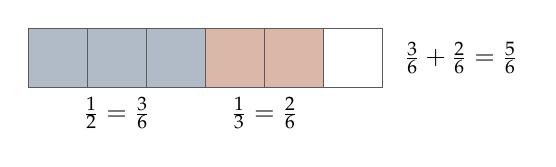
\begin{tikzpicture}[x=0.75cm,y=0.75cm,font=\small]
\foreach \i in {0,...,5} {\draw[linie] (\i,0) rectangle (\i+1,1);}
\fill[tief!35] (0,0) rectangle (3,1);
\fill[akzent!40] (3,0) rectangle (5,1);
\foreach \i in {0,...,5} {\draw[grau] (\i,0) rectangle (\i+1,1);}
\node[below] at (1.5,0) {$\frac12 = \frac36$};
\node[below] at (4,0) {$\frac13 = \frac26$};
\node[right] at (6.2,0.5) {$\frac36 + \frac26 = \frac56$};
\end{tikzpicture}
\end{center}
Fünf von sechs Feldern sind gefärbt. $\frac25$ wäre weniger als die Hälfte --- aber allein $\frac12$ ist schon die Hälfte, und es kommt etwas dazu. Eine Summe zweier positiver Brüche ist größer als jeder Summand; $\frac25 < \frac12$ kann also nicht stimmen.
\schritt{(b)}
$\frac{1 + 1}{2 + 3}$ ist der \emph{Mediant}: Trifft man $1$ von $2$ Würfen und dann $1$ von $3$, hat man insgesamt $2$ von $5$ getroffen. Das ist eine gemeinsame Trefferquote, keine Summe von Anteilen --- und sie liegt immer \emph{zwischen} den beiden Quoten ($\frac13 < \frac25 < \frac12$), nie darüber.
\schritt{(c)}
Nein. $x = 2$: $\frac{4}{6} = \frac23$, aber $\frac{x + 1}{x + 2} = \frac34$. Die $2$ und die $4$ sind Summanden, keine Faktoren.
\schritt{(d)}
Kürzen heißt, einen gemeinsamen \emph{Faktor} von Zähler und Nenner zu entfernen: $\frac{ac}{bc} = \frac ab$. Aus Summen kürzt nur, wer zuerst ausklammert --- und dann einen Faktor hat.
\probe{$\frac{2x + 4}{2x + 8} = \frac{2(x + 2)}{2(x + 4)} = \frac{x + 2}{x + 4}$: hier \emph{darf} man die $2$ kürzen, weil sie Faktor beider Seiten ist. \checkmark}
\begin{fehler}\kastentext
\enquote{Zähler plus Zähler, Nenner plus Nenner.} Es sieht aus wie eine Regel, ist aber die Rechnung für etwas anderes (den Medianten). Das Ergebnis liegt zwischen den Brüchen, statt größer als beide zu sein --- daran erkennt man den Fehler sofort.
\end{fehler}
\begin{mitnehmen}\kastentext
Drei Verbote, eine Regel: Nur Faktoren kürzen, nur Gleichnamiges addieren, nur über Produkte Wurzeln und Potenzen verteilen. Summen lassen nichts mit sich machen, außer dass man sie zusammenfasst.
\end{mitnehmen}
\end{loesungkarte}

%%%%%%%%%%%%%%%%%%%%%%%%%%%%%%%%%%%%%%%%%%%%%%%%%% 0.7
\stupserzwei{gruen}{Erste Klammer: Hauptnenner $12$, Ergebnis negativ. Zweite Klammer: Hauptnenner $12$, Ergebnis $\frac34$.}{22pt}
\begin{loesungkarte}{gruen}{0.7}{Kürzen bis zum Ende}
\derweg{Klammern zuerst, dann die Division als Multiplikation mit dem Kehrwert, dann alles in einen Bruch und kürzen.}
\schritt{(a)}
$\frac34 - \frac56 = \frac9{12} - \frac{10}{12} = -\frac1{12}$. \quad $\frac23 + \frac1{12} = \frac8{12} + \frac1{12} = \frac9{12} = \frac34$.
\[ -\frac1{12} : \frac34\cdot\frac59 = -\frac1{12}\cdot\frac43\cdot\frac59 = -\frac{1\cdot4\cdot5}{12\cdot3\cdot9} = -\frac{20}{324} = -\frac5{81} . \]
Schneller: die $4$ gegen die $12$ kürzen, bevor man multipliziert: $-\frac1{3}\cdot\frac13\cdot\frac59 = -\frac5{81}$.
\schritt{(b)}
$(0{,}750 - 0{,}833) : (0{,}667 + 0{,}083)\cdot0{,}556 = (-0{,}083) : 0{,}750\cdot0{,}556 = -0{,}111\cdot0{,}556 = -0{,}0617$; und $-\frac5{81} = -0{,}0617$. \checkmark
\probe{Die Division geht \emph{vor} der Multiplikation, weil sie links steht: $a : b\cdot c = (a : b)\cdot c$. Hätte man $a : (b\cdot c)$ gerechnet, käme $-\frac1{12} : \frac{15}{36} = -\frac15$ heraus --- falsch.}
\begin{mitnehmen}\kastentext
Punktrechnung von links nach rechts; und kürzen, bevor man multipliziert, hält die Zahlen klein.
\end{mitnehmen}
\end{loesungkarte}

%%%%%%%%%%%%%%%%%%%%%%%%%%%%%%%%%%%%%%%%%%%%%%%%%% 0.8
\stupserzwei{tief}{$1{,}2\cdot0{,}8 = 0{,}96$. Die zwanzig Prozent nach oben wurden von einer kleineren Zahl genommen als die zwanzig nach unten.}{22pt}
\begin{loesungkarte}{tief}{0.8}{Zwanzig Prozent hin, zwanzig zurück}
\derweg{Jede Prozentänderung ist ein Faktor; Hintereinander heißt Produkt.}
\schritt{(a)}
$1{,}2\cdot0{,}8 = 0{,}96$: Es bleiben $96\,\%$, der Preis ist um $4\,\%$ gefallen. Konkret: $100\to120\to96$.
\schritt{(b)}
Gesucht $q$ mit $1{,}2\cdot q = 1$, also $q = \frac1{1{,}2} = 0{,}8\overline3$: Der Preis muss um $16{,}7\,\%$ sinken. Die Umkehrung einer Erhöhung um $p\,\%$ ist eine Senkung um $\frac{p}{100 + p}\cdot100\,\%$, nicht um $p\,\%$.
\schritt{(c)}
$1{,}15^{2} = 1{,}3225$: $32{,}25\,\%$, nicht $30$. Die zweite Erhöhung wirkt auch auf die erste --- \enquote{Zinseszins}. Der Unterschied $2{,}25\,\% = 0{,}15^{2}$ ist das Produkt der beiden Raten.
\schritt{(d)}
Von $5$ auf $6$: ein Prozent\emph{punkt} mehr; relativ $\frac65 = 1{,}2$, also $20\,\%$ Anstieg. Beide Angaben sind richtig und meinen Verschiedenes --- und Schlagzeilen wählen die größere.
\probe{(b): $120\cdot0{,}8\overline3 = 100$. \checkmark\ (a) allgemein: $(1 + p)(1 - p) = 1 - p^{2} < 1$ für jedes $p\neq0$ --- hin und zurück verliert immer.}
\begin{mitnehmen}\kastentext
Prozent sind Faktoren: plus $p\,\%$ ist $\times(1 + \frac p{100})$. Hintereinander wird multipliziert, rückgängig wird dividiert, und Prozentpunkte sind Differenzen, keine Faktoren.
\end{mitnehmen}
\end{loesungkarte}

%%%%%%%%%%%%%%%%%%%%%%%%%%%%%%%%%%%%%%%%%%%%%%%%%% 0.9
\stupserzwei{tief}{$(2a^{2}b^{-1})^{3} = 8a^{6}b^{-3}$ und $(ab^{2})^{-2} = a^{-2}b^{-4}$. Dann Exponenten von $a$ und $b$ je zusammenzählen.}{22pt}
\begin{loesungkarte}{tief}{0.9}{Potenzen aufräumen}
\derweg{Klammern einzeln potenzieren, dann je Basis die Exponenten addieren beziehungsweise subtrahieren.}
\schritt{(a)}
\[ \frac{8a^{6}b^{-3}\cdot a^{-2}b^{-4}}{4a} = \frac{8}{4}\cdot a^{6 - 2 - 1}\cdot b^{-3 - 4} = 2a^{3}b^{-7} = \frac{2a^{3}}{b^{7}} . \]
\schritt{(b)}
$\sqrt[3]{x^{2}} = x^{2/3}$, $\sqrt x = x^{1/2}$; Produkt $x^{2/3 + 1/2} = x^{7/6} = x\sqrt[6]x$.
\schritt{(c)}
Aus $a^{m}\cdot a^{0} = a^{m + 0} = a^{m}$ folgt $a^{0} = 1$ (für $a\neq0$). Aus $a^{n}\cdot a^{-n} = a^{0} = 1$ folgt $a^{-n} = 1/a^{n}$. Die Definitionen sind so gewählt, dass das eine Gesetz für alle ganzen Exponenten gilt --- das ist der einzige Grund.
\probe{(a) mit $a = 2$, $b = 3$: links $\frac{(8/3)^{3}\cdot(18)^{-2}}{8} = \frac{18{,}963\cdot0{,}003086}{8} = 0{,}007316$; rechts $\frac{16}{2187} = 0{,}007316$. \checkmark}
\begin{mitnehmen}\kastentext
Alle Potenzgesetze sind Buchhaltung über Exponenten; die Definitionen von $a^{0}$, $a^{-n}$, $a^{1/n}$ sind so gemacht, dass die Buchhaltung nie eine Ausnahme braucht.
\end{mitnehmen}
\end{loesungkarte}

%%%%%%%%%%%%%%%%%%%%%%%%%%%%%%%%%%%%%%%%%%%%%%%%%% 0.10
\stupserzwei{tief}{$2^{x} = 16 = 2^{4}$. Bei (c) ist $\ln x + \ln(x - 3) = \ln\bigl(x(x - 3)\bigr)$, und gleiche Logarithmen heißen gleiche Argumente.}{22pt}
\begin{loesungkarte}{tief}{0.10}{Die Unbekannte im Exponenten}
\derweg{Potenz isolieren, Logarithmus anwenden; bei Logarithmengleichungen zuerst zu einem Logarithmus zusammenfassen und am Ende den Definitionsbereich prüfen.}
\schritt{(a)}
$2^{x} = 16 = 2^{4}$, also $x = 4$.
\schritt{(b)}
$(2x - 1)\ln3 = \ln7$, also $x = \frac12\bigl(\frac{\ln7}{\ln3} + 1\bigr) = \frac12(1{,}7712 + 1) = 1{,}386$.
\schritt{(c)}
$\ln\bigl(x(x - 3)\bigr) = \ln10$, also $x^{2} - 3x - 10 = 0$, $x = 5$ oder $x = -2$. Für $x = -2$ ist $\ln x$ nicht definiert: einzige Lösung $x = 5$. Probe: $\ln5 + \ln2 = \ln10$. \checkmark
\schritt{(d)}
Weil $\ln a + \ln b = \ln(ab)$ ist, nicht $\ln(a + b)$. Der Logarithmus macht aus Produkten Summen --- das ist sein Zweck ---, und daher aus Summen nichts Einfaches. (Dieselbe Regel wie in Aufgabe 0.2: Operationen verteilen sich nicht über Summen.)
\probe{(b): $3^{2\cdot1{,}386 - 1} = 3^{1{,}772} = e^{1{,}772\cdot1{,}0986} = e^{1{,}946} = 7{,}00$. \checkmark}
\begin{mitnehmen}\kastentext
Logarithmieren holt die Unbekannte aus dem Exponenten --- aber nur, wenn die Potenz allein steht. Und bei Logarithmengleichungen gehört die Probe zur Lösung, weil das Zusammenfassen Kandidaten erzeugt, die nicht im Definitionsbereich liegen.
\end{mitnehmen}
\end{loesungkarte}

%%%%%%%%%%%%%%%%%%%%%%%%%%%%%%%%%%%%%%%%%%%%%%%%%% 0.11
\stupserzwei{gruen}{$64 = 2^{6}$, $\frac19 = 3^{-2}$, $\sqrt5 = 5^{1/2}$. Bei (d): $1{,}03^{t} = 2$, beide Seiten $\ln$.}{22pt}
\begin{loesungkarte}{gruen}{0.11}{Logarithmen ohne Rechner}
\derweg{Die Zahl als Potenz der Basis schreiben; die Rechenregeln sind die Potenzgesetze, rückwärts gelesen.}
\schritt{(a)}
$\log_264 = 6$, $\log_3\frac19 = -2$, $\log_5\sqrt5 = \frac12$.
\schritt{(b)}
$\log_a(x^{3}y) - 2\log_ax + \log_a\frac1y = 3\log_ax + \log_ay - 2\log_ax - \log_ay = \log_ax$.
\schritt{(c)}
Sei $c = \log_ab$, also $a^{c} = b$. Logarithmieren: $c\ln a = \ln b$, also $c = \frac{\ln b}{\ln a}$. Damit $\log_210 = \frac{\ln10}{\ln2} = \frac{2{,}3026}{0{,}6931} = 3{,}322$. (Probe: $2^{3} = 8 < 10 < 16 = 2^{4}$. \checkmark)
\schritt{(d)}
$1{,}03^{t} = 2$, also $t = \frac{\ln2}{\ln1{,}03} = \frac{0{,}6931}{0{,}02956} = 23{,}4$ Jahre. Faustregel $70/3 = 23{,}3$. Sie beruht auf $\ln2\approx0{,}70$ und $\ln(1 + p)\approx p$ für kleine $p$.
\probe{(b) mit $a = 10$, $x = 10$, $y = 100$: $\log(10^{5}) - 2 + \log(0{,}01) = 5 - 2 - 2 = 1 = \log10$. \checkmark}
\begin{mitnehmen}\kastentext
$\log_ab$ ist die Antwort auf \enquote{$a$ hoch was gibt $b$?} --- alle Regeln folgen aus dieser Frage, und die Basisumrechnung macht aus jedem Logarithmus einen natürlichen.
\end{mitnehmen}
\end{loesungkarte}

%%%%%%%%%%%%%%%%%%%%%%%%%%%%%%%%%%%%%%%%%%%%%%%%%% 0.12
\stupserzwei{akzent}{$1{,}01^{100}\approx2{,}70$. Die Verdopplung: $1{,}01^{t} = 2$, also $t = \ln2/\ln1{,}01$. Die Seerose: einen Tag vor dem Ende war sie halb so groß.}{22pt}
\begin{loesungkarte}{akzent}{0.12}{Ein Prozent am Tag}
\derweg{Wachstum um einen festen Prozentsatz ist Multiplikation mit einem festen Faktor; über $t$ Schritte ist das eine Potenz.}
\schritt{(a)}
$1{,}01^{100} = 2{,}705$: ein Zuwachs von $170\,\%$, nicht $100$. Der Unterschied ist der Zuwachs auf den Zuwachs.
\schritt{(b)}
$1{,}01^{t} = 2$ gibt $t = \frac{\ln2}{\ln1{,}01} = \frac{0{,}6931}{0{,}00995} = 69{,}7$ Tage. Faustregel $70/1 = 70$. \checkmark
\schritt{(c)}
Verdopplung täglich heißt rückwärts Halbierung täglich: halb bedeckt an Tag $29$, zu einem Viertel an Tag $28$. Wer am Tag $28$ sagt \enquote{drei Viertel sind noch frei}, hat zwei Tage.
\schritt{(d)}
$N(t) = N_0\cdot1{,}01^{t}$. Der Zuwachs von Tag $t$ auf $t + 1$ ist $N(t + 1) - N(t) = 0{,}01\cdot N(t)$ --- ein fester \emph{Anteil} des jeweiligen Bestands, also ein wachsender Betrag. Linear wäre $N_0(1 + 0{,}01t)$: fester Betrag $0{,}01N_0$ je Tag.
\begin{center}
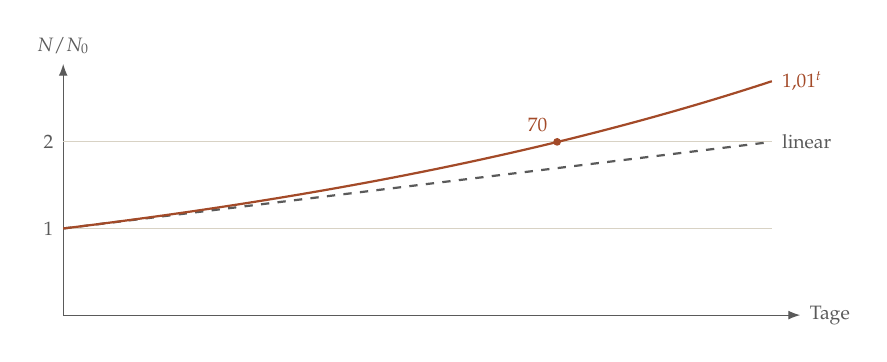
\begin{tikzpicture}[x=0.09cm,y=1.1cm,font=\small]
\draw[grau,-{Latex[length=1.5mm]}] (0,0)--(104,0) node[right,font=\scriptsize]{Tage};
\draw[grau,-{Latex[length=1.5mm]}] (0,0)--(0,2.9) node[above,font=\scriptsize]{$N/N_0$};
\foreach \y in {1,2} {\draw[linie] (0,\y)--(100,\y); \node[left,font=\scriptsize,grau] at (0,\y) {\y};}
\draw[grau,thick,dashed] (0,1)--(100,2) node[right,font=\scriptsize,grau]{linear};
\draw[akzent,thick] plot[domain=0:100,samples=50] (\x,{1.01^\x}) node[right,font=\scriptsize,akzent]{$1{,}01^{t}$};
\fill[akzent] (69.7,2) circle (1.4pt); \node[akzent,font=\scriptsize,above left] at (69.7,2) {$70$};
\end{tikzpicture}
\end{center}
\probe{(a) über die Verdopplungszeit: $100/69{,}7 = 1{,}435$ Verdopplungen, $2^{1{,}435} = 2{,}70$. \checkmark}
\begin{fehler}\kastentext
\enquote{Ein Prozent pro Tag, hundert Tage, also hundert Prozent.} --- Das addiert Prozente, die sich auf verschiedene Grundwerte beziehen. Der zweite Tag bringt ein Prozent von $1{,}01N_0$, nicht von $N_0$. Je länger die Zeit, desto größer der Fehler: nach $700$ Tagen ist der Bestand das Tausendfache, nicht das Achtfache.
\end{fehler}
\begin{mitnehmen}\kastentext
Exponentielles Wachstum erkennt man daran, dass die \emph{Verdopplungszeit} konstant ist, nicht der Zuwachs. Faustregel: $70$ durch Prozentsatz. Kapitel 8 in Band 0, Band 18 für Populationen, Band 3 für die Theorie.
\end{mitnehmen}
\end{loesungkarte}

%%%%%%%%%%%%%%%%%%%%%%%%%%%%%%%%%%%%%%%%%%%%%%%%%% 0.13
\stupserzwei{gruen}{$x^{2} - 9 = (x - 3)(x + 3)$, $x^{2} - 6x + 9 = (x - 3)^{2}$, $x^{2} - 3x = x(x - 3)$, $x^{2} + 3x = x(x + 3)$.}{22pt}
\begin{loesungkarte}{gruen}{0.13}{Ein Bruchterm wird eins}
\derweg{Alle vier Polynome faktorisieren, Nullstellen der Nenner notieren, dann Faktoren kürzen.}
\schritt{(a)}
\[ \frac{(x - 3)(x + 3)}{(x - 3)^{2}}\cdot\frac{x(x - 3)}{x(x + 3)} = \frac{(x - 3)(x + 3)\cdot x(x - 3)}{(x - 3)^{2}\cdot x(x + 3)} = 1 . \]
\schritt{(b)}
Nenner null für $x = 3$ (erster Bruch) und $x = 0$, $x = -3$ (zweiter). Definitionsbereich $\mathbb R\setminus\{-3, 0, 3\}$. Der Term ist \emph{nicht} die konstante Funktion $1$, sondern $1$ mit drei Löchern: An den Stellen $-3$, $0$, $3$ ist er nicht definiert, auch wenn das gekürzte Ergebnis es nicht mehr zeigt. Die Information über den Definitionsbereich geht beim Kürzen verloren, deshalb liest man ihn vorher ab.
\probe{$x = 1$: $\frac{1 - 9}{1 - 6 + 9}\cdot\frac{1 - 3}{1 + 3} = \frac{-8}{4}\cdot\frac{-2}{4} = (-2)(-\tfrac12) = 1$. \checkmark}
\begin{mitnehmen}\kastentext
Erst faktorisieren, dann den Definitionsbereich notieren, dann kürzen --- in dieser Reihenfolge. Ein gekürzter Term hat ein kürzeres Gedächtnis als der ursprüngliche.
\end{mitnehmen}
\end{loesungkarte}

%%%%%%%%%%%%%%%%%%%%%%%%%%%%%%%%%%%%%%%%%%%%%%%%%% 0.14
\stupserzwei{tief}{$2x^{2} - 8x + 3 = 2(x^{2} - 4x) + 3 = 2\bigl((x - 2)^{2} - 4\bigr) + 3$. Genau eine Lösung heißt Diskriminante null.}{22pt}
\begin{loesungkarte}{tief}{0.14}{Quadratisch: faktorisieren, ergänzen, lesen}
\derweg{Drei Formen derselben Funktion --- Produkt, Scheitelpunkt, Summe ---, und jede Frage hat ihre Form.}
\schritt{(a)}
Gesucht zwei Zahlen mit Produkt $6$ und Summe $5$: $2$ und $3$. $x^{2} - 5x + 6 = (x - 2)(x - 3)$, Lösungen $x = 2$ und $x = 3$.
\schritt{(b)}
$2x^{2} - 8x + 3 = 2(x^{2} - 4x) + 3 = 2\bigl((x - 2)^{2} - 4\bigr) + 3 = 2(x - 2)^{2} - 5$. Scheitel $(2, -5)$, Parabel nach oben geöffnet, Wertebereich $[-5, \infty)$.
\schritt{(c)}
Der Scheitel liegt unterhalb der Achse und die Parabel öffnet nach oben: zwei Nullstellen. Direkt aus der Form: $2(x - 2)^{2} = 5$, $x = 2\pm\sqrt{5/2} = 2\pm1{,}58$.
\schritt{(d)}
$x^{2} - 6x + c = (x - 3)^{2} + c - 9$; genau eine Lösung, wenn der Scheitel auf der Achse liegt: $c = 9$. Gleichbedeutend: Diskriminante $36 - 4c = 0$.
\begin{center}
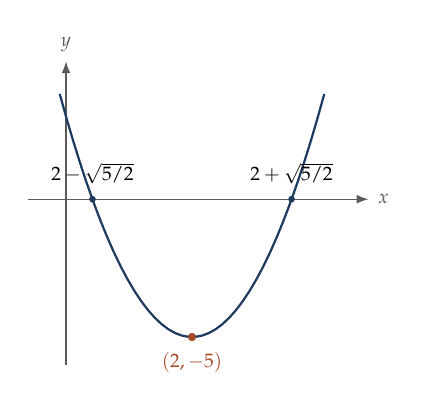
\begin{tikzpicture}[x=0.8cm,y=0.35cm,font=\small]
\draw[grau,-{Latex[length=1.5mm]}] (-0.6,0)--(4.8,0) node[right,font=\scriptsize]{$x$};
\draw[grau,-{Latex[length=1.5mm]}] (0,-6)--(0,5) node[above,font=\scriptsize]{$y$};
\draw[tief,thick] plot[domain=-0.1:4.1,samples=40] (\x,{2*(\x-2)^2-5});
\fill[akzent] (2,-5) circle (1.5pt); \node[akzent,font=\scriptsize,below] at (2,-5.2) {$(2, -5)$};
\fill[tief] (0.42,0) circle (1.2pt); \fill[tief] (3.58,0) circle (1.2pt);
\node[font=\scriptsize,above] at (0.42,0.2) {$2 - \sqrt{5/2}$}; \node[font=\scriptsize,above] at (3.58,0.2) {$2 + \sqrt{5/2}$};
\end{tikzpicture}
\end{center}
\probe{(a) Vieta: $2 + 3 = 5$, $2\cdot3 = 6$. \checkmark\ (b) ausmultiplizieren: $2(x^{2} - 4x + 4) - 5 = 2x^{2} - 8x + 3$. \checkmark}
\begin{mitnehmen}\kastentext
Faktorisierte Form: Nullstellen. Scheitelpunktform: Extremum, Wertebereich, Zahl der Nullstellen. Die $p$-$q$-Formel braucht man erst, wenn beides nicht zu sehen ist.
\end{mitnehmen}
\end{loesungkarte}

%%%%%%%%%%%%%%%%%%%%%%%%%%%%%%%%%%%%%%%%%%%%%%%%%% 0.15
\stupserzwei{gruen}{(b): Hauptnenner $(x - 2)(x + 2)$; die Lösung $x = 2$ fällt weg, weil sie den Nenner null macht. (c): $x$ muss $\ge0$ sein, bevor man quadriert.}{22pt}
\begin{loesungkarte}{gruen}{0.15}{Vier Gleichungen, vier Methoden}
\derweg{Jede Gleichung auf eine Normalform bringen, die man kennt --- und jede Umformung, die nicht umkehrbar ist, mit der Probe bezahlen.}
\schritt{(a)}
Durch $2$: $x^{2} - 5x + 6 = 0$, also $x = 2$ oder $x = 3$ (Aufgabe 0.14a). Probe: $8 - 20 + 12 = 0$, $18 - 30 + 12 = 0$. \checkmark
\schritt{(b)}
$x^{2} - 4 = (x - 2)(x + 2)$; Definitionsbereich $x\neq\pm2$. Mal $(x - 2)(x + 2)$: $x(x + 2) + 3(x - 2) = 8$, also $x^{2} + 5x - 14 = 0$, $(x + 7)(x - 2) = 0$. $x = 2$ ist ausgeschlossen. Einzige Lösung $x = -7$. Probe: $\frac{-7}{-9} + \frac3{-5} = \frac79 - \frac35 = \frac{35 - 27}{45} = \frac8{45}$; rechts $\frac8{49 - 4} = \frac8{45}$. \checkmark
\schritt{(c)}
Quadrieren: $2x + 3 = x^{2}$, also $x^{2} - 2x - 3 = 0$, $(x - 3)(x + 1) = 0$. Probe: $x = 3$: $\sqrt9 = 3$. \checkmark\ $x = -1$: $\sqrt1 = 1\neq-1$. Scheinlösung --- sie löst $-\sqrt{2x + 3} = x$, die Gleichung, die beim Quadrieren dieselbe wird. Lösung $x = 3$.
\schritt{(d)}
$4^{x} = (2^{x})^{2}$; mit $u = 2^{x}$: $u^{2} - 5u + 4 = 0$, $u = 1$ oder $u = 4$, also $x = 0$ oder $x = 2$. Probe: $1 - 5 + 4 = 0$; $16 - 20 + 4 = 0$. \checkmark
\schritt{Warum die Probe bei (b) und (c) Pflicht ist}
Multiplizieren mit einem Term, der null werden kann, und Quadrieren sind keine Äquivalenzumformungen: Sie können Lösungen hinzufügen (nie wegnehmen). Die Probe filtert die hinzugefügten heraus. Bei (a) und (d) wurde nur durch Konstanten geteilt und substituiert --- umkehrbar, Probe freiwillig.
\begin{mitnehmen}\kastentext
Äquivalenzumformung: Probe ist Kür. Quadrieren, mit Variablen multiplizieren, Logarithmen zusammenfassen: Probe ist Pflicht, weil die neue Gleichung mehr Lösungen haben kann als die alte.
\end{mitnehmen}
\end{loesungkarte}

%%%%%%%%%%%%%%%%%%%%%%%%%%%%%%%%%%%%%%%%%%%%%%%%%% 0.16
\stupserzwei{akzent}{$\sqrt{16} = 4$, auch wenn die $16$ von $-4$ kam. Also $\sqrt{x^{2}} = |x|$. Und $x^{2} = 9$ hat zwei Lösungen, weil zwei Zahlen das Quadrat $9$ haben.}{22pt}
\begin{loesungkarte}{akzent}{0.16}{Wurzeln, Beträge, Scheinlösungen}
\derweg{Die Wurzel ist eine Funktion mit nichtnegativen Werten; Quadrieren ist keine Funktion rückwärts --- daher der Betrag, die zwei Lösungen, die Scheinlösung.}
\schritt{(a)}
$\sqrt{4^{2}} = \sqrt{16} = 4$ und $\sqrt{(-4)^{2}} = \sqrt{16} = 4$. Allgemein $\sqrt{x^{2}} = |x|$. Die Wurzel \enquote{weiß} nicht mehr, ob $x$ negativ war.
\schritt{(b)}
$x^{2} = 9$ heißt $|x| = 3$, also $x = 3$ oder $x = -3$. Nicht nur $\sqrt9 = 3$: Die Wurzel gibt die nichtnegative Lösung, die Gleichung hat beide.
\schritt{(c)}
$\sqrt{9 + 16} = 5$, aber $3 + 4 = 7$. Gleichheit $\sqrt{a^{2} + b^{2}} = a + b$ würde nach Quadrieren $a^{2} + b^{2} = a^{2} + 2ab + b^{2}$ verlangen, also $ab = 0$: nur wenn eine der Zahlen null ist. (Geometrisch: die Hypotenuse ist kürzer als die Summe der Katheten --- Dreiecksungleichung.)
\schritt{(d)}
Quadrieren: $x + 2 = x^{2}$, $x^{2} - x - 2 = (x - 2)(x + 1) = 0$. $x = 2$: $\sqrt4 = 2$. \checkmark\ $x = -1$: $\sqrt1 = 1\neq-1$. Im Bild: Die Gerade $y = x$ schneidet die Wurzelkurve $y = \sqrt{x + 2}$ einmal, bei $x = 2$; die Parabel $y^{2} = x + 2$ (beide Wurzeläste) schneidet sie zweimal. Die Scheinlösung $x = -1$ liegt auf dem \emph{unteren} Ast $y = -\sqrt{x + 2}$, den die Gleichung nie gemeint hat.
\begin{center}
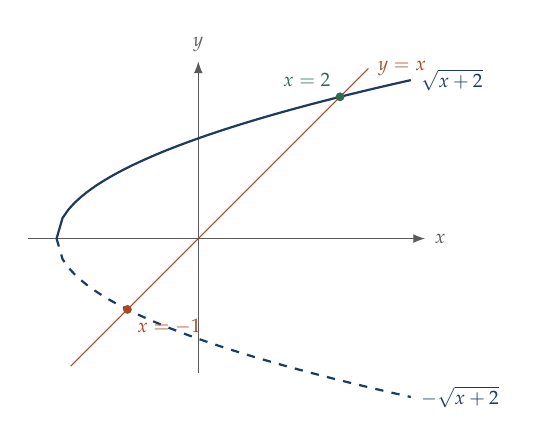
\begin{tikzpicture}[x=0.9cm,y=0.9cm,font=\small]
\draw[grau,-{Latex[length=1.5mm]}] (-2.4,0)--(3.2,0) node[right,font=\scriptsize]{$x$};
\draw[grau,-{Latex[length=1.5mm]}] (0,-1.9)--(0,2.5) node[above,font=\scriptsize]{$y$};
\draw[tief,thick] plot[domain=-2:3,samples=60] (\x,{sqrt(\x+2)}) node[right,font=\scriptsize,tief]{$\sqrt{x + 2}$};
\draw[tief,thick,dashed] plot[domain=-2:3,samples=60] (\x,{-sqrt(\x+2)}) node[right,font=\scriptsize,tief]{$-\sqrt{x + 2}$};
\draw[akzent] (-1.8,-1.8)--(2.4,2.4) node[right,font=\scriptsize,akzent]{$y = x$};
\fill[gruen] (2,2) circle (1.6pt); \node[gruen,font=\scriptsize,above left] at (2,2) {$x = 2$};
\fill[akzent] (-1,-1) circle (1.6pt); \node[akzent,font=\scriptsize,below right] at (-1,-1) {$x = -1$};
\end{tikzpicture}
\end{center}
\probe{(c) allgemein: $\sqrt{a^{2} + b^{2}}\le a + b$ für $a, b\ge0$, mit Gleichheit nur für $ab = 0$. \checkmark}
\begin{fehler}\kastentext
\enquote{$\sqrt{x^{2}} = x$.} --- Für negative $x$ falsch; richtig ist $|x|$. Daraus folgen beide anderen Fehler: Wer $\sqrt{x^{2}} = x$ glaubt, sieht nur eine Lösung von $x^{2} = 9$ und hält die Scheinlösung von $\sqrt{x + 2} = x$ für echt.
\end{fehler}
\begin{mitnehmen}\kastentext
$\sqrt{\ }$ ist eine Funktion: ein Eingang, ein nichtnegativer Ausgang. Quadrieren ist nicht ihre Umkehrung auf ganz $\mathbb R$ --- und jede Rechnung, die so tut, braucht am Ende die Probe.
\end{mitnehmen}
\end{loesungkarte}

%%%%%%%%%%%%%%%%%%%%%%%%%%%%%%%%%%%%%%%%%%%%%%%%%% 0.17
\stupserzwei{tief}{Aus $x - y = 1$ folgt $x = y + 1$; das in die erste Gleichung. Oder: zweite Gleichung mal $3$ und zur ersten addieren --- $y$ verschwindet.}{22pt}
\begin{loesungkarte}{tief}{0.17}{Zwei Gleichungen, zwei Unbekannte}
\derweg{Eine Unbekannte eliminieren --- durch Einsetzen oder durch Addition ---, die andere ausrechnen, zurück einsetzen.}
\schritt{(a) Einsetzen}
$x = y + 1$ in $2x + 3y = 12$: $2y + 2 + 3y = 12$, $5y = 10$, $y = 2$, $x = 3$.
\schritt{(a) Addition}
Zweite Gleichung mal $3$: $3x - 3y = 3$. Plus erste: $5x = 15$, $x = 3$, dann $y = 2$. Probe: $6 + 6 = 12$, $3 - 2 = 1$. \checkmark
\schritt{(b)}
$4x + 6y = 20$ ist das Doppelte der linken Seite von $2x + 3y = 12$, aber $20\neq24$: Widerspruch, keine Lösung. $4x + 6y = 24$ ist genau das Doppelte: dieselbe Gleichung zweimal, unendlich viele Lösungen --- alle Punkte der Geraden $2x + 3y = 12$.
\schritt{(c)}
Zwei Geraden schneiden sich in einem Punkt (eine Lösung), sind parallel (keine) oder fallen zusammen (unendlich viele). Parallel heißt: gleiche Steigung, verschiedener Achsenabschnitt --- genau der Fall $20\neq24$.
\begin{center}
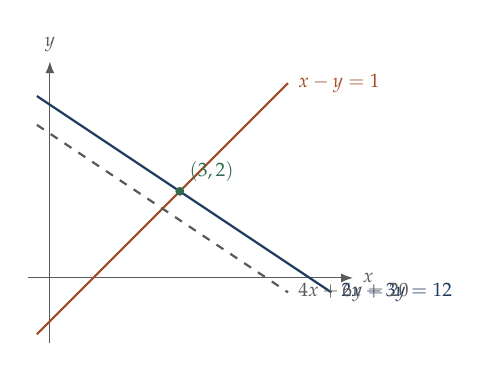
\begin{tikzpicture}[x=0.55cm,y=0.55cm,font=\small]
\draw[grau,-{Latex[length=1.5mm]}] (-0.5,0)--(7,0) node[right,font=\scriptsize]{$x$};
\draw[grau,-{Latex[length=1.5mm]}] (0,-1.5)--(0,5) node[above,font=\scriptsize]{$y$};
\draw[tief,thick] plot[domain=-0.3:6.5] (\x,{(12-2*\x)/3}) node[right,font=\scriptsize,tief]{$2x + 3y = 12$};
\draw[akzent,thick] plot[domain=-0.3:5.5] (\x,{\x-1}) node[right,font=\scriptsize,akzent]{$x - y = 1$};
\draw[grau,thick,dashed] plot[domain=-0.3:5.5] (\x,{(20-4*\x)/6}) node[right,font=\scriptsize,grau]{$4x + 6y = 20$};
\fill[gruen] (3,2) circle (1.6pt); \node[gruen,font=\scriptsize,above right] at (3,2) {$(3, 2)$};
\end{tikzpicture}
\end{center}
\begin{mitnehmen}\kastentext
Ein lineares System mit zwei Unbekannten ist ein Bild aus zwei Geraden. Band 2 macht daraus Matrizen; die drei Fälle --- eine, keine, unendlich viele Lösungen --- bleiben dieselben.
\end{mitnehmen}
\end{loesungkarte}

%%%%%%%%%%%%%%%%%%%%%%%%%%%%%%%%%%%%%%%%%%%%%%%%%% 0.18
\stupserzwei{akzent}{$-2x > 6$ heißt $x < -3$: Beim Teilen durch $-2$ dreht sich das Zeichen. $x^{2} = 3x$ heißt $x^{2} - 3x = 0$, also $x(x - 3) = 0$ --- zwei Faktoren, zwei Lösungen.}{22pt}
\begin{loesungkarte}{akzent}{0.18}{Mal minus, durch $x$}
\derweg{Statt zu teilen, bringt man alles auf eine Seite und faktorisiert; und bei Ungleichungen merkt man sich, dass negative Faktoren die Ordnung umkehren.}
\schritt{(a)}
$-2x + 5 > 11$, also $-2x > 6$, also $x < -3$. Probe: $x = -4$: $8 + 5 = 13 > 11$. \checkmark\ $x = 0$: $5 > 11$ falsch. \checkmark\ Warum sich das Zeichen dreht: $2 < 3$, aber $-2 > -3$ --- Multiplikation mit $-1$ spiegelt die Zahlengerade und vertauscht links und rechts.
\schritt{(b)}
$x^{2} - 3x = 0$, $x(x - 3) = 0$: $x = 0$ oder $x = 3$. Wer beide Seiten durch $x$ teilt, setzt stillschweigend $x\neq0$ voraus und verliert die Lösung $x = 0$.
\schritt{(c)}
Für $x > 0$: $6 > 2x$, $x < 3$, also $0 < x < 3$. Für $x < 0$: Multiplikation dreht das Zeichen, $6 < 2x$, $x > 3$ --- Widerspruch zu $x < 0$, keine Lösung. Insgesamt $0 < x < 3$. Wer ohne Fallunterscheidung multipliziert, bekommt $x < 3$ und erklärt $x = -1$ zur Lösung; aber $\frac6{-1} = -6 > 2$ ist falsch.
\schritt{(d)}
Multipliziert oder dividiert man eine Ungleichung mit einer Zahl, deren Vorzeichen man nicht kennt, muss man die Fälle unterscheiden. Dividiert man eine Gleichung durch einen Term, der null sein könnte, muss man den Fall \enquote{gleich null} getrennt prüfen.
\begin{fehler}\kastentext
\enquote{Durch $x$ teilen} und \enquote{mit $x$ multiplizieren} sehen harmlos aus. Das eine verschluckt $x = 0$, das andere ignoriert das Vorzeichen. Beide Fehler vermeidet, wer faktorisiert statt teilt und Fälle unterscheidet statt multipliziert.
\end{fehler}
\begin{mitnehmen}\kastentext
$ab = 0$ heißt $a = 0$ oder $b = 0$ --- das ist der sichere Weg. Und bei Ungleichungen: Vorzeichen unbekannt, Fall unterscheiden.
\end{mitnehmen}
\end{loesungkarte}

%%%%%%%%%%%%%%%%%%%%%%%%%%%%%%%%%%%%%%%%%%%%%%%%%% 0.19
\stupserzwei{gruen}{(a): $-4\le2x - 6\le4$, dann $+6$ und $:2$. (b): Für $x > 3$ darf man multiplizieren, ohne zu drehen; für $x < 3$ dreht sich das Zeichen.}{22pt}
\begin{loesungkarte}{gruen}{0.19}{Betrag und Bruch in Ungleichungen}
\derweg{Betrag als Doppelungleichung lesen; Bruch nach dem Vorzeichen des Nenners in Fälle teilen.}
\schritt{(a)}
$|2x - 6|\le4$ heißt $-4\le2x - 6\le4$, also $2\le2x\le10$, also $1\le x\le5$. Deutung: $|2x - 6| = 2|x - 3|$, der Abstand von $x$ zu $3$ ist höchstens $2$.
\schritt{(b)}
Fall $x > 3$ (Nenner positiv): $x + 1\ge2(x - 3) = 2x - 6$, also $x\le7$. Zusammen $3 < x\le7$. Fall $x < 3$ (Nenner negativ, Zeichen dreht): $x + 1\le2x - 6$, also $x\ge7$ --- Widerspruch zu $x < 3$. Lösung: $(3, 7]$. Die $3$ selbst ist ausgeschlossen (Nenner null), die $7$ gehört dazu ($\frac87 \cdot$ --- $\frac{8}{4} = 2\ge2$ \checkmark).
\begin{center}
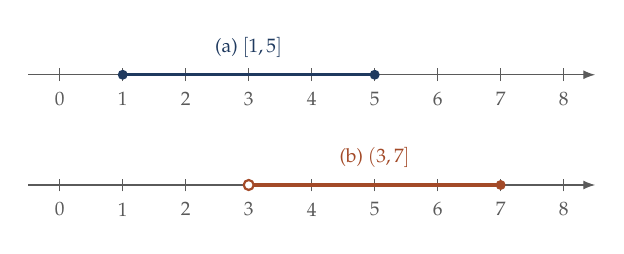
\begin{tikzpicture}[x=0.8cm,font=\small]
\draw[grau,-{Latex[length=1.5mm]}] (-0.5,0.8)--(8.5,0.8);
\foreach \x in {0,...,8} {\draw[grau] (\x,0.72)--(\x,0.88); \node[below,font=\scriptsize,grau] at (\x,0.7) {\x};}
\draw[tief,very thick] (1,0.8)--(5,0.8); \fill[tief] (1,0.8) circle (1.8pt); \fill[tief] (5,0.8) circle (1.8pt);
\node[tief,font=\scriptsize,above] at (3,0.9) {(a) $[1, 5]$};
\draw[grau,-{Latex[length=1.5mm]}] (-0.5,-0.6)--(8.5,-0.6);
\foreach \x in {0,...,8} {\draw[grau] (\x,-0.68)--(\x,-0.52); \node[below,font=\scriptsize,grau] at (\x,-0.7) {\x};}
\draw[akzent,very thick] (3,-0.6)--(7,-0.6); \draw[akzent,fill=white,thick] (3,-0.6) circle (1.8pt); \fill[akzent] (7,-0.6) circle (1.8pt);
\node[akzent,font=\scriptsize,above] at (5,-0.5) {(b) $(3, 7]$};
\end{tikzpicture}
\end{center}
\probe{(b) mit $x = 5$: $\frac62 = 3\ge2$. \checkmark\ Mit $x = 8$: $\frac95 = 1{,}8 < 2$. \checkmark\ Mit $x = 0$: $\frac1{-3} < 2$, nicht in der Lösungsmenge. \checkmark}
\begin{mitnehmen}\kastentext
$|a|\le r$ heißt $-r\le a\le r$; $|a|\ge r$ heißt $a\le-r$ oder $a\ge r$. Und ein Bruch in einer Ungleichung verlangt immer die Frage nach dem Vorzeichen des Nenners.
\end{mitnehmen}
\end{loesungkarte}

%%%%%%%%%%%%%%%%%%%%%%%%%%%%%%%%%%%%%%%%%%%%%%%%%% 0.20
\stupserzwei{tief}{Unter der Wurzel $x - 1\ge0$. Die Wurzel ist mindestens $0$, also $f(x)\ge2$. Umkehren: $y = \sqrt{x - 1} + 2$, nach $x$ auflösen --- und $y\ge2$ mitnehmen.}{22pt}
\begin{loesungkarte}{tief}{0.20}{Eine Funktion lesen}
\derweg{Definitionsbereich aus der Wurzel, Wertebereich aus dem kleinsten Wert, Umkehrfunktion durch Auflösen --- und die Bereiche tauschen die Rollen.}
\schritt{(a)}
$D = [1, \infty)$; $\sqrt{x - 1}$ durchläuft $[0, \infty)$, also $W = [2, \infty)$.
\schritt{(b)}
Der Graph von $\sqrt x$, um $1$ nach rechts und $2$ nach oben verschoben: Er beginnt im Punkt $(1, 2)$.
\schritt{(c)}
$y = \sqrt{x - 1} + 2$, also $\sqrt{x - 1} = y - 2$, also $x = (y - 2)^{2} + 1$ --- gültig für $y\ge2$. $f^{-1}(x) = (x - 2)^{2} + 1$ mit Definitionsbereich $[2, \infty)$ (dem Wertebereich von $f$). Ohne diese Einschränkung wäre $f^{-1}$ eine ganze Parabel und keine Umkehrfunktion.
\begin{center}
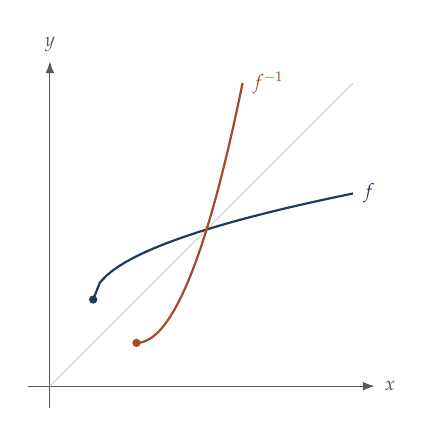
\begin{tikzpicture}[x=0.55cm,y=0.55cm,font=\small]
\draw[grau,-{Latex[length=1.5mm]}] (-0.5,0)--(7.5,0) node[right,font=\scriptsize]{$x$};
\draw[grau,-{Latex[length=1.5mm]}] (0,-0.5)--(0,7.5) node[above,font=\scriptsize]{$y$};
\draw[linie] (0,0)--(7,7);
\draw[tief,thick] plot[domain=1:7,samples=40] (\x,{sqrt(\x-1)+2}) node[right,font=\scriptsize,tief]{$f$};
\draw[akzent,thick] plot[domain=2:4.45,samples=40] (\x,{(\x-2)^2+1}) node[right,font=\scriptsize,akzent]{$f^{-1}$};
\fill[tief] (1,2) circle (1.5pt); \fill[akzent] (2,1) circle (1.5pt);
\end{tikzpicture}
\end{center}
\schritt{(d)}
$f(5) = \sqrt4 + 2 = 4$, $f^{-1}(4) = 4 + 1 = 5$. \checkmark\ $f^{-1}(3) = 1 + 1 = 2$, $f(2) = 1 + 2 = 3$. \checkmark
\begin{mitnehmen}\kastentext
Der Graph der Umkehrfunktion ist die Spiegelung an der Diagonalen --- und mitgespiegelt werden die Bereiche: $D$ wird $W$, $W$ wird $D$. Wer den Wertebereich nicht bestimmt, bekommt eine falsche Umkehrfunktion.
\end{mitnehmen}
\end{loesungkarte}

%%%%%%%%%%%%%%%%%%%%%%%%%%%%%%%%%%%%%%%%%%%%%%%%%% 0.21
\stupserzwei{gruen}{$f(x) = 2$ hätte $2x - 1 = 2x + 6$ zur Folge --- unmöglich. Die $2$ ist der Wert, den $f$ nie erreicht: die waagerechte Asymptote.}{22pt}
\begin{loesungkarte}{gruen}{0.21}{Umkehren und zurück}
\derweg{Der Nenner gibt die Definitionslücke, die Asymptote gibt die Lücke im Wertebereich, Auflösen nach $x$ gibt die Umkehrfunktion --- mit vertauschten Lücken.}
\schritt{(a)}
$D = \mathbb R\setminus\{-3\}$. Wertebereich: $y = \frac{2x - 1}{x + 3}$ nach $x$ auflösen: $y(x + 3) = 2x - 1$, $x(y - 2) = -3y - 1$, $x = \frac{-3y - 1}{y - 2}$ --- für jedes $y\neq2$ gibt es genau ein $x$. $W = \mathbb R\setminus\{2\}$. ($2$ ist der Grenzwert für $x\to\pm\infty$.)
\schritt{(b)}
Die Auflösung in (a) ist eindeutig: Zu jedem $y$ genau ein $x$, also injektiv. $f^{-1}(y) = \frac{-3y - 1}{y - 2} = \frac{3y + 1}{2 - y}$, Definitionsbereich $\mathbb R\setminus\{2\}$, Wertebereich $\mathbb R\setminus\{-3\}$.
\schritt{(c)}
\[ f^{-1}\bigl(f(x)\bigr) = \frac{3\cdot\frac{2x - 1}{x + 3} + 1}{2 - \frac{2x - 1}{x + 3}} = \frac{\frac{6x - 3 + x + 3}{x + 3}}{\frac{2x + 6 - 2x + 1}{x + 3}} = \frac{7x}{7} = x .\ \checkmark \]
\probe{$f(0) = -\frac13$, $f^{-1}(-\frac13) = \frac{-1 + 1}{2 + \frac13} = 0$. \checkmark\ $f(1) = \frac14$, $f^{-1}(\frac14) = \frac{\frac74}{\frac74} = 1$. \checkmark}
\begin{mitnehmen}\kastentext
Bei gebrochen-linearen Funktionen stehen Definitionslücke und Asymptote in den Koeffizienten: $x = -\frac dc$, $y = \frac ac$. Die Umkehrfunktion vertauscht sie. Und \enquote{Verkettung gibt $x$} ist die Probe, die keine Ausrede zulässt.
\end{mitnehmen}
\end{loesungkarte}

%%%%%%%%%%%%%%%%%%%%%%%%%%%%%%%%%%%%%%%%%%%%%%%%%% 0.22
\stupserzwei{gruen}{$15$ Stunden sind $2{,}5$ Halbwertszeiten: zweimal halbieren und dann noch einmal durch $\sqrt2$. $50 = 400/8 = 400/2^{3}$: drei Halbwertszeiten.}{22pt}
\begin{loesungkarte}{gruen}{0.22}{Halbwertszeit}
\derweg{Die Zeit in Halbwertszeiten messen; dann ist der Rest eine Potenz von $\frac12$, und \enquote{wann?} ist ein Logarithmus zur Basis $2$.}
\schritt{(a)}
$N(t) = 400\cdot\bigl(\tfrac12\bigr)^{t/6}$ mg, $t$ in Stunden. Gleichwertig $400\cdot e^{-\lambda t}$ mit $\lambda = \frac{\ln2}6 = 0{,}1155$ h$^{-1}$.
\schritt{(b)}
$t = 15$: $400\cdot2^{-2{,}5} = 400/(4\sqrt2) = 400/5{,}657 = 70{,}7$ mg.
\schritt{(c)}
$400\cdot2^{-t/6} = 50$, also $2^{-t/6} = \frac18 = 2^{-3}$, $t = 18$ h --- drei Halbwertszeiten, ohne Rechner.
\schritt{(d)}
$2^{-t/6} = \frac1{400}$, also $t = 6\log_2400 = 6\cdot\frac{\ln400}{\ln2} = 6\cdot8{,}644 = 51{,}9$ h. Nach rund $52$ Stunden --- knapp neun Halbwertszeiten, denn $2^{9} = 512 > 400$.
\begin{center}
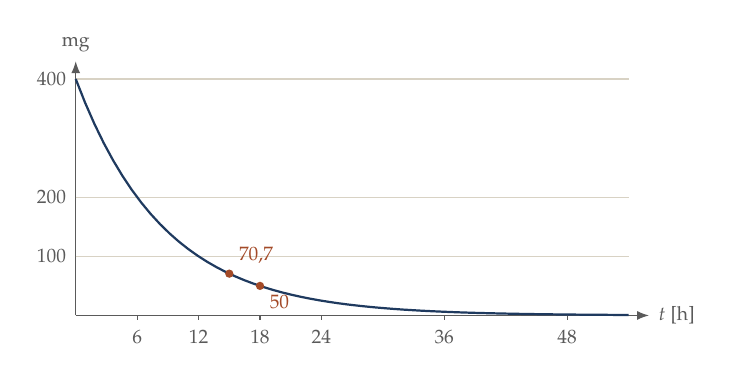
\begin{tikzpicture}[x=0.13cm,y=0.0075cm,font=\small]
\draw[grau,-{Latex[length=1.5mm]}] (0,0)--(56,0) node[right,font=\scriptsize]{$t$ [h]};
\draw[grau,-{Latex[length=1.5mm]}] (0,0)--(0,430) node[above,font=\scriptsize]{mg};
\foreach \y in {100,200,400} {\draw[linie] (0,\y)--(54,\y); \node[left,font=\scriptsize,grau] at (0,\y) {\y};}
\foreach \x in {6,12,18,24,36,48} {\draw[grau] (\x,0)--(\x,-8); \node[below,font=\scriptsize,grau] at (\x,-8) {\x};}
\draw[tief,thick] plot[domain=0:54,samples=60] (\x,{400*0.5^(\x/6)});
\fill[akzent] (15,70.7) circle (1.5pt); \node[akzent,font=\scriptsize,above right] at (15,70.7) {$70{,}7$};
\fill[akzent] (18,50) circle (1.5pt); \node[akzent,font=\scriptsize,below right] at (18,50) {$50$};
\end{tikzpicture}
\end{center}
\probe{(b) über (a): $N(12) = 100$, $N(18) = 50$, dazwischen bei $15$: $100/\sqrt2 = 70{,}7$. \checkmark}
\begin{mitnehmen}\kastentext
Halbwertszeit als Zeiteinheit: Nach $k$ Halbwertszeiten ist $2^{-k}$ übrig. Fünf Halbwertszeiten sind $3\,\%$ --- die Faustregel für \enquote{praktisch eliminiert}. Band 18 rechnet so mit Medikamentenspiegeln, Band 14 mit der Differentialgleichung dahinter.
\end{mitnehmen}
\end{loesungkarte}

%%%%%%%%%%%%%%%%%%%%%%%%%%%%%%%%%%%%%%%%%%%%%%%%%% 0.23
\stupserzwei{akzent}{$120$ km hin bei $60$ km/h: $2$ Stunden. Zurück bei $40$: $3$ Stunden. $240$ km in $5$ Stunden.}{22pt}
\begin{loesungkarte}{akzent}{0.23}{Hin mit 60, zurück mit 40}
\derweg{Durchschnittsgeschwindigkeit ist Gesamtstrecke durch Gesamtzeit --- und die langsamere Hälfte dauert länger, also zählt sie mehr.}
\schritt{(a)}
Strecke $s$ je Richtung: Zeiten $\frac s{60}$ und $\frac s{40}$. Mittel $= \frac{2s}{s/60 + s/40} = \frac{2}{1/60 + 1/40} = \frac2{5/120} = 48$ km/h. Nicht $50$, weil man mehr Zeit mit $40$ unterwegs ist als mit $60$.
\schritt{(b)}
$s$ kürzt sich heraus: $\bar v = \dfrac{2}{\frac1{v_1} + \frac1{v_2}} = \dfrac{2v_1v_2}{v_1 + v_2}$ --- das \emph{harmonische} Mittel. (Vergleiche Aufgabe 0.5b: $\frac{ab}{a + b}$, doppelt.)
\schritt{(c)}
Mengen gleich, Raten $100$ und $50$ ml/h: harmonisches Mittel $\frac{2\cdot100\cdot50}{150} = 66{,}7$ ml/h. Probe mit $200$ ml: $100$ ml in $1$ h, $100$ ml in $2$ h, $200$ ml in $3$ h $= 66{,}7$ ml/h. \checkmark
\schritt{(d)}
Das arithmetische Mittel ist richtig, wenn die \emph{Zeiten} gleich sind: eine Stunde $60$, eine Stunde $40$ ergibt $100$ km in $2$ h $= 50$ km/h. Bei gleichen Strecken (oder Mengen) ist es das harmonische. Allgemein: Man mittelt die Größe, die im Zähler steht, über die, die im Nenner steht.
\begin{fehler}\kastentext
\enquote{$(60 + 40)/2 = 50$.} --- Das arithmetische Mittel gewichtet beide Fahrten gleich; tatsächlich dauert die langsame länger. Das harmonische Mittel ist immer kleiner als das arithmetische (hier $48 < 50$), und der Unterschied wächst mit dem Abstand der Werte.
\end{fehler}
\begin{mitnehmen}\kastentext
Bevor man mittelt: Was ist gleich --- Strecke oder Zeit, Menge oder Dauer? Gleiche Zähler: harmonisch. Gleiche Nenner: arithmetisch. Band 17 kennt noch das geometrische Mittel für Wachstumsraten.
\end{mitnehmen}
\end{loesungkarte}

%%%%%%%%%%%%%%%%%%%%%%%%%%%%%%%%%%%%%%%%%%%%%%%%%% 0.24
\stupserzwei{gruen}{Mantellinie $s = \sqrt{36 + 64} = 10$. Oberer Teilkegel: Faktor $k$ mit $k^{3} = \frac12$, also $k = 0{,}794$; seine Höhe ist $8k$.}{22pt}
\begin{loesungkarte}{gruen}{0.24}{Der halbe Kegel}
\derweg{Volumen und Oberfläche nach Formel; für den Schnitt die Ähnlichkeit: der obere Teil ist ein Kegel mit allen Längen mal $k$, also Volumen mal $k^{3}$.}
\schritt{(a)}
$V = \frac13\pi r^{2}h = \frac13\pi\cdot36\cdot8 = 96\pi\approx301{,}6$ cm$^{3}$. Mantellinie $s = \sqrt{r^{2} + h^{2}} = \sqrt{36 + 64} = 10$ cm. Oberfläche $O = \pi r^{2} + \pi rs = 36\pi + 60\pi = 96\pi\approx301{,}6$ cm$^{2}$. (Dass $V$ und $O$ dieselbe Maßzahl haben, ist Zufall --- ein Kegel mit $r = 6$, $h = 8$ ist eben so gebaut.)
\schritt{(b)}
Schneidet man in der Höhe $x$ über der Grundfläche, ist der obere Teil ein Kegel der Höhe $8 - x$, ähnlich zum ganzen mit Faktor $k = \frac{8 - x}8$. Sein Volumen ist $k^{3}V$. Gleiche Volumina: $k^{3} = \frac12$, $k = \sqrt[3]{1/2} = 0{,}7937$. Also $8 - x = 6{,}35$, $x = 1{,}65$ cm über der Grundfläche --- viel tiefer als die halbe Höhe, weil der Kegel unten breit ist.
\begin{center}
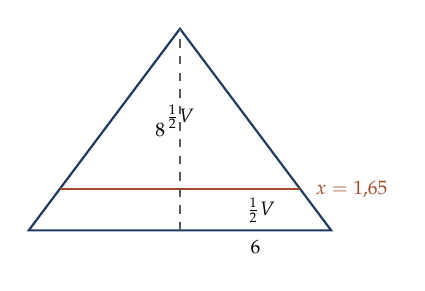
\begin{tikzpicture}[x=0.32cm,y=0.32cm,font=\small]
\draw[tief,thick] (-6,0)--(6,0)--(0,8)--cycle;
\draw[akzent,thick] (-4.76,1.65)--(4.76,1.65);
\draw[grau,dashed] (0,0)--(0,8);
\node[akzent,font=\scriptsize,right] at (5,1.65) {$x = 1{,}65$};
\node[font=\scriptsize,left] at (-0.2,4) {$8$};
\node[font=\scriptsize,below] at (3,0) {$6$};
\node[font=\scriptsize] at (0,4.5) {$\tfrac12V$};
\node[font=\scriptsize] at (3.2,0.8) {$\tfrac12V$};
\end{tikzpicture}
\end{center}
\probe{Oberer Kegel: Radius $6k = 4{,}76$, Höhe $6{,}35$, Volumen $\frac13\pi\cdot22{,}68\cdot6{,}35 = 150{,}8 = \frac12\cdot301{,}6$. \checkmark}
\begin{mitnehmen}\kastentext
Längen mal $k$, Flächen mal $k^{2}$, Volumina mal $k^{3}$. Das ist der Grund, warum man einen Kegel nicht in halber Höhe halbiert, warum große Tiere dicke Beine haben und warum Dosierungen nach Körperoberfläche und nicht nach Gewicht gehen (Band 18).
\end{mitnehmen}
\end{loesungkarte}

%%%%%%%%%%%%%%%%%%%%%%%%%%%%%%%%%%%%%%%%%%%%%%%%%% 0.25
\stupserzwei{tief}{$150^{\circ}$ liegt im zweiten Quadranten, Bezugswinkel $30^{\circ}$: Sinus positiv. $240^{\circ}$ im dritten, Bezugswinkel $60^{\circ}$: Kosinus negativ.}{22pt}
\begin{loesungkarte}{tief}{0.25}{Am Einheitskreis}
\derweg{Winkel zeichnen, Bezugswinkel zur $x$-Achse bestimmen, Vorzeichen aus dem Quadranten.}
\schritt{(a)}
$\sin150^{\circ} = \sin30^{\circ} = \frac12$. $\cos240^{\circ} = -\cos60^{\circ} = -\frac12$. $\tan315^{\circ} = \frac{\sin315^{\circ}}{\cos315^{\circ}} = \frac{-\sqrt2/2}{\sqrt2/2} = -1$.
\schritt{(b)}
$\sin x = -\frac12$: $y$-Koordinate $-\frac12$, also unten; Bezugswinkel $30^{\circ} = \frac\pi6$. Dritter und vierter Quadrant: $x = \pi + \frac\pi6 = \frac{7\pi}6$ und $x = 2\pi - \frac\pi6 = \frac{11\pi}6$.
\schritt{(c)}
$\cos x = \frac12$: die senkrechte Gerade $x = \frac12$ schneidet den Kreis zweimal ($\pm\frac\pi3$). $\sin x = 1$: die waagerechte Gerade $y = 1$ berührt den Kreis nur im höchsten Punkt $\frac\pi2$. Zwei Lösungen, wenn der Wert echt zwischen $-1$ und $1$ liegt; eine am Rand; keine außerhalb.
\begin{center}
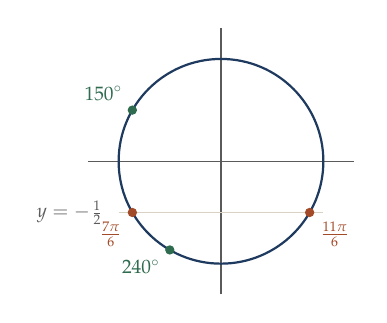
\begin{tikzpicture}[scale=1.3,font=\small]
\draw[grau] (-1.3,0)--(1.3,0); \draw[grau] (0,-1.3)--(0,1.3);
\draw[tief,thick] (0,0) circle (1);
\draw[linie] (-1,-0.5)--(1,-0.5);
\fill[akzent] (-0.866,-0.5) circle (1.3pt) node[below left,font=\scriptsize] {$\frac{7\pi}6$};
\fill[akzent] (0.866,-0.5) circle (1.3pt) node[below right,font=\scriptsize] {$\frac{11\pi}6$};
\node[font=\scriptsize,grau,left] at (-1.05,-0.5) {$y = -\frac12$};
\fill[gruen] (-0.866,0.5) circle (1.3pt) node[above left,font=\scriptsize] {$150^{\circ}$};
\fill[gruen] (-0.5,-0.866) circle (1.3pt) node[below left,font=\scriptsize] {$240^{\circ}$};
\end{tikzpicture}
\end{center}
\begin{mitnehmen}\kastentext
Der Einheitskreis ist die Tabelle: Bezugswinkel liefert den Betrag, Quadrant das Vorzeichen, Symmetrie die zweite Lösung. Band 3 und Band 12 bauen darauf die Analysis der Winkelfunktionen.
\end{mitnehmen}
\end{loesungkarte}

%%%%%%%%%%%%%%%%%%%%%%%%%%%%%%%%%%%%%%%%%%%%%%%%%% 0.26
\stupserzwei{gruen}{$c^{2} = a^{2} + b^{2} - 2ab\cos\gamma$. Bei (c): $\sin2x = 2\sin x\cos x$, dann $\cos x$ ausklammern --- nicht durch $\cos x$ teilen (Aufgabe 0.18).}{22pt}
\begin{loesungkarte}{gruen}{0.26}{Ein Dreieck ohne rechten Winkel}
\derweg{Kosinussatz für die Seite, Sinussatz für den kleineren Winkel, Winkelsumme für den Rest; Fläche aus zwei Seiten und dem eingeschlossenen Winkel.}
\schritt{(a)}
$c^{2} = 49 + 81 - 2\cdot7\cdot9\cdot\cos52^{\circ} = 130 - 126\cdot0{,}6157 = 130 - 77{,}57 = 52{,}43$, $c = 7{,}24$ cm. Sinussatz für den Winkel gegenüber der \emph{kleineren} Seite $a$ (sicher spitz): $\sin\alpha = \frac{a\sin\gamma}{c} = \frac{7\cdot0{,}7880}{7{,}24} = 0{,}7618$, $\alpha = 49{,}6^{\circ}$. Dann $\beta = 180^{\circ} - 52^{\circ} - 49{,}6^{\circ} = 78{,}4^{\circ}$.
\schritt{(b)}
$F = \frac12ab\sin\gamma = \frac12\cdot63\cdot0{,}7880 = 24{,}8$ cm$^{2}$.
\schritt{(c)}
$\sin2x = 2\sin x\cos x$, also $2\sin x\cos x - \cos x = 0$, $\cos x\,(2\sin x - 1) = 0$. Entweder $\cos x = 0$: $x = \frac\pi2, \frac{3\pi}2$; oder $\sin x = \frac12$: $x = \frac\pi6, \frac{5\pi}6$. Vier Lösungen. Wer durch $\cos x$ teilt, verliert die ersten beiden.
\probe{(a) Sinussatz für $\beta$: $\frac{9\cdot0{,}7880}{7{,}24} = 0{,}9795$, $\beta = 78{,}4^{\circ}$. \checkmark\ (c) $x = \frac\pi2$: $\sin\pi = 0 = \cos\frac\pi2$. \checkmark}
\begin{mitnehmen}\kastentext
Zwei Seiten und der eingeschlossene Winkel: Kosinussatz zuerst. Den Sinussatz immer für den Winkel gegenüber der kleineren Seite --- er ist spitz, und der Arkussinus gibt ihn richtig. Und Produkt gleich null ist sicherer als dividieren.
\end{mitnehmen}
\end{loesungkarte}

%%%%%%%%%%%%%%%%%%%%%%%%%%%%%%%%%%%%%%%%%%%%%%%%%% 0.27
\stupserzwei{gruen}{(b): $(\sqrt{n^{2} + n} - n)\cdot\frac{\sqrt{n^{2} + n} + n}{\sqrt{n^{2} + n} + n} = \frac{n}{\sqrt{n^{2} + n} + n}$. Dann durch $n$ kürzen.}{22pt}
\begin{loesungkarte}{gruen}{0.27}{Vier Grenzwerte}
\derweg{Durch die höchste Potenz kürzen; Wurzeldifferenzen mit der dritten binomischen Formel; geometrische Reihe $\sum q^{k} = \frac1{1 - q}$.}
\schritt{(a)}
$\dfrac{3 - 5/n + 2/n^{2}}{2 + 7/n}\to\dfrac32$.
\schritt{(b)}
Erweitern: $\dfrac{(n^{2} + n) - n^{2}}{\sqrt{n^{2} + n} + n} = \dfrac{n}{\sqrt{n^{2} + n} + n} = \dfrac{1}{\sqrt{1 + 1/n} + 1}\to\dfrac12$.
\schritt{(c)}
$q = \frac23$, $|q| < 1$: Summe $\frac1{1 - 2/3} = 3$.
\schritt{(d)}
$0{,}\overline7 = \frac7{10} + \frac7{100} + \dots = \frac7{10}\sum_{k\ge0}\bigl(\frac1{10}\bigr)^{k} = \frac7{10}\cdot\frac{1}{1 - 1/10} = \frac7{10}\cdot\frac{10}9 = \frac79$. Exakt, nicht näherungsweise: Der Grenzwert der Partialsummen \emph{ist} $\frac79$.
\probe{(b) numerisch $n = 100$: $\sqrt{10100} - 100 = 100{,}499 - 100 = 0{,}499$. \checkmark\ (d): $7 : 9 = 0{,}777\ldots$ \checkmark}
\begin{mitnehmen}\kastentext
$0{,}\overline9 = 1$ aus demselben Grund: $\frac9{10}\cdot\frac{10}9$. Eine unendliche Dezimalzahl ist eine Reihe, und eine Reihe ist ein Grenzwert --- Band 3, Kapitel 2.
\end{mitnehmen}
\end{loesungkarte}

%%%%%%%%%%%%%%%%%%%%%%%%%%%%%%%%%%%%%%%%%%%%%%%%%% 0.28
\stupserzwei{tief}{$f'(x) = 3x^{2} - 3$. Nullstellen von $f$ in $[0, 2]$: $x = 0$ und $x = \sqrt3$. Dazwischen ist $f$ negativ --- das Integral zählt die Fläche dort mit Minus.}{22pt}
\begin{loesungkarte}{tief}{0.28}{Tangente, Extrema, Fläche}
\derweg{Ableitung ausrechnen, an der Stelle auswerten; Nullstellen der Ableitung; für die Fläche das Integral an den Nullstellen von $f$ zerlegen.}
\schritt{(a)}
$f(2) = 8 - 6 = 2$, $f'(x) = 3x^{2} - 3$, $f'(2) = 9$. Tangente $y = 2 + 9(x - 2) = 9x - 16$.
\schritt{(b)}
$f'(x) = 0$ für $x = \pm1$. $f''(x) = 6x$: $f''(1) = 6 > 0$, Minimum bei $(1, -2)$; $f''(-1) < 0$, Maximum bei $(-1, 2)$.
\schritt{(c)}
$\int_0^{2}(x^{3} - 3x)\,dx = \bigl[\tfrac{x^{4}}4 - \tfrac{3x^{2}}2\bigr]_0^{2} = 4 - 6 = -2$. Nullstellen von $f$: $x(x^{2} - 3) = 0$, in $[0, 2]$ bei $0$ und $\sqrt3$. $\int_0^{\sqrt3}f = \frac94 - \frac92 = -\frac94$ (unter der Achse), $\int_{\sqrt3}^{2}f = -2 - (-\frac94) = \frac14$ (darüber). Fläche $= \frac94 + \frac14 = \frac52$. Das Integral $-2$ ist die \emph{Bilanz} der beiden Teile, die Fläche ihre Summe.
\begin{center}
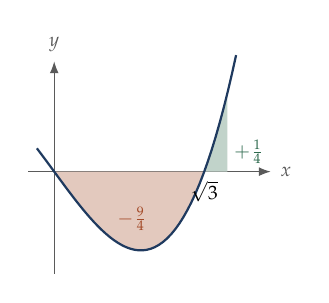
\begin{tikzpicture}[x=1.1cm,y=0.5cm,font=\small]
\draw[grau,-{Latex[length=1.5mm]}] (-0.3,0)--(2.5,0) node[right,font=\scriptsize]{$x$};
\draw[grau,-{Latex[length=1.5mm]}] (0,-2.6)--(0,2.8) node[above,font=\scriptsize]{$y$};
\fill[akzent!30] plot[domain=0:1.732,samples=30] (\x,{\x^3-3*\x}) -- (1.732,0) -- (0,0) -- cycle;
\fill[gruen!30] plot[domain=1.732:2,samples=20] (\x,{\x^3-3*\x}) -- (2,0) -- (1.732,0) -- cycle;
\draw[tief,thick] plot[domain=-0.2:2.1,samples=50] (\x,{\x^3-3*\x});
\node[akzent,font=\scriptsize] at (0.9,-1.2) {$-\frac94$};
\node[gruen,font=\scriptsize] at (2.25,0.5) {$+\frac14$};
\node[font=\scriptsize,below] at (1.732,0) {$\sqrt3$};
\end{tikzpicture}
\end{center}
\probe{(a): die Tangente trifft $f$ bei $x = 2$: $9\cdot2 - 16 = 2 = f(2)$. \checkmark\ (c): $-\frac94 + \frac14 = -2$. \checkmark}
\begin{mitnehmen}\kastentext
Das Integral ist eine Bilanz mit Vorzeichen; die Fläche ist die Summe der Beträge. Wer Flächen will, braucht die Nullstellen zuerst --- Band 3, Kapitel 8.
\end{mitnehmen}
\end{loesungkarte}

%%%%%%%%%%%%%%%%%%%%%%%%%%%%%%%%%%%%%%%%%%%%%%%%%% 0.29
\stupserzwei{gruen}{$-\frac2x = -2x^{-1}$ hat Ableitung $2x^{-2}$; $5\sqrt x = 5x^{1/2}$ hat Ableitung $\frac52x^{-1/2}$. Innen mal außen bei der Kette.}{22pt}
\begin{loesungkarte}{gruen}{0.29}{Vier Ableitungen}
\derweg{Umschreiben, Regel wählen, rechnen, aufräumen.}
\schritt{(a)}
$f'(x) = 12x^{3} + \dfrac2{x^{2}} + \dfrac5{2\sqrt x}$.
\schritt{(b)}
Produktregel: $g'(x) = 2xe^{-x} + x^{2}(-e^{-x}) = (2x - x^{2})e^{-x} = x(2 - x)e^{-x}$.
\schritt{(c)}
Quotientenregel: $h'(x) = \dfrac{x\cos x - \sin x}{x^{2}}$.
\schritt{(d)}
Kettenregel: $k'(x) = \dfrac{1}{2\sqrt{3x^{2} + 1}}\cdot6x = \dfrac{3x}{\sqrt{3x^{2} + 1}}$.
\probe{(b) hat Nullstellen der Ableitung bei $x = 0$ und $x = 2$: $g$ hat dort Minimum ($g(0) = 0$) und Maximum ($g(2) = 4e^{-2} = 0{,}54$). \checkmark\ (d) numerisch bei $x = 1$: $\frac{k(1{,}001) - k(1)}{0{,}001} = \frac{2{,}0015 - 2}{0{,}001} = 1{,}50$; Formel $\frac3{2} = 1{,}5$. \checkmark}
\begin{mitnehmen}\kastentext
Vier Regeln, immer dieselbe Frage vorab: Ist das eine Summe, ein Produkt, ein Quotient oder eine Verkettung? Die Antwort steht fest, bevor man rechnet.
\end{mitnehmen}
\end{loesungkarte}

%%%%%%%%%%%%%%%%%%%%%%%%%%%%%%%%%%%%%%%%%%%%%%%%%% 0.30
\stupserzwei{gruen}{Stammfunktion von $\frac4{x + 1}$ ist $4\ln(x + 1)$. Schnittpunkte von $x^{2}$ und $2x$: $0$ und $2$. Kugel: $\pi\int_{-r}^{r}(r^{2} - x^{2})\,dx$.}{22pt}
\begin{loesungkarte}{gruen}{0.30}{Drei Integrale}
\derweg{Stammfunktion und Grenzen; Fläche zwischen Kurven ist Integral der Differenz; Rotationsvolumen ist $\pi\int y^{2}$.}
\schritt{(a)}
$\int_1^{3}\bigl(2x^{2} - \tfrac4{x + 1}\bigr)dx = \bigl[\tfrac{2x^{3}}3 - 4\ln(x + 1)\bigr]_1^{3} = \bigl(18 - 4\ln4\bigr) - \bigl(\tfrac23 - 4\ln2\bigr) = \tfrac{52}3 - 4\ln2 = 17{,}33 - 2{,}77 = 14{,}56$.
\schritt{(b)}
$x^{2} = 2x$ bei $x = 0$ und $x = 2$; dazwischen ist $2x > x^{2}$. Fläche $\int_0^{2}(2x - x^{2})\,dx = \bigl[x^{2} - \tfrac{x^{3}}3\bigr]_0^{2} = 4 - \tfrac83 = \tfrac43$.
\schritt{(c)}
Der Halbkreis $y = \sqrt{r^{2} - x^{2}}$, $-r\le x\le r$, rotiert um die $x$-Achse: $V = \pi\int_{-r}^{r}(r^{2} - x^{2})\,dx = \pi\bigl[r^{2}x - \tfrac{x^{3}}3\bigr]_{-r}^{r} = \pi\bigl(2r^{3} - \tfrac{2r^{3}}3\bigr) = \tfrac43\pi r^{3}$.
\probe{(a) grob: der Integrand liegt zwischen $0$ ($x = 1$) und $17$ ($x = 3$), Mittel etwa $7$ auf einem Intervall der Länge $2$: $\approx14$. \checkmark\ (b) ist $\frac13$ des umschließenden Rechtecks $2\times4$ --- wie bei jeder Parabel über einer Sehne (Archimedes). \checkmark}
\begin{mitnehmen}\kastentext
Fläche zwischen Kurven: Schnittpunkte, dann obere minus untere. Rotationsvolumen: Scheiben vom Radius $y$, also $\pi y^{2}$ aufsummiert. Beides ist der Hauptsatz, einmal angewandt.
\end{mitnehmen}
\end{loesungkarte}

%%%%%%%%%%%%%%%%%%%%%%%%%%%%%%%%%%%%%%%%%%%%%%%%%% 0.31
\stupserzwei{gruen}{$n^{2} + (2n + 1) = n^{2} + 2n + 1 = (n + 1)^{2}$ --- die erste binomische Formel ist der ganze Induktionsschritt.}{22pt}
\begin{loesungkarte}{gruen}{0.31}{Die ungeraden Zahlen}
\derweg{Anfang prüfen, dann zeigen: Wenn die Formel für $n$ gilt, gilt sie für $n + 1$. Das Bild erklärt, warum; die Induktion beweist, dass.}
\schritt{(a)}
$1 = 1$; $1 + 3 = 4$; $1 + 3 + 5 = 9$; $1 + 3 + 5 + 7 = 16$. \checkmark
\schritt{(b)}
\emph{Anfang} $n = 1$: $1 = 1^{2}$. \emph{Schritt}: Gelte $1 + 3 + \dots + (2n - 1) = n^{2}$. Dann
\[ 1 + 3 + \dots + (2n - 1) + (2n + 1) = n^{2} + 2n + 1 = (n + 1)^{2}, \]
und $2n + 1 = 2(n + 1) - 1$ ist die nächste ungerade Zahl. Also gilt die Formel für $n + 1$, und damit für alle $n\ge1$. $\blacksquare$
\schritt{(c)}
\begin{center}
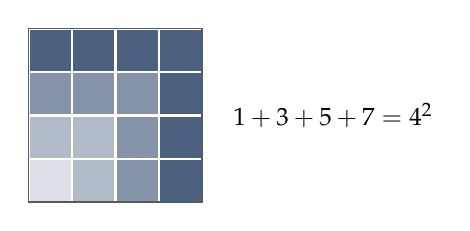
\begin{tikzpicture}[x=0.55cm,y=0.55cm]
\foreach \k/\c in {0/tief!15,1/tief!35,2/tief!55,3/tief!80} {
  \foreach \i in {0,...,\k} {\fill[\c] (\i,\k) rectangle (\i+1,\k+1); \fill[\c] (\k,\i) rectangle (\k+1,\i+1);}
}
\foreach \i in {0,...,4} {\draw[white,thick] (\i,0)--(\i,4); \draw[white,thick] (0,\i)--(4,\i);}
\draw[grau] (0,0) rectangle (4,4);
\node[right,font=\small] at (4.5,2) {$1 + 3 + 5 + 7 = 4^{2}$};
\end{tikzpicture}
\end{center}
Jeder Winkel (\enquote{Gnomon}) fügt die nächste ungerade Zahl hinzu und macht aus dem $n\times n$-Quadrat ein $(n + 1)\times(n + 1)$-Quadrat. Das Bild \emph{ist} der Induktionsschritt, anschaulich: Es zeigt, warum $n^{2} + (2n + 1) = (n + 1)^{2}$. Ein Beweis ist es nicht, weil es nur ein $n$ zeigt und man glauben muss, dass es für alle so weitergeht --- genau das, was die Induktion statt des Glaubens liefert.
\begin{mitnehmen}\kastentext
Induktion ist die Dominoreihe: Der erste fällt, und jeder stößt den nächsten um. Das Bild zeigt, warum ein Stein den nächsten umstößt; der Beweis stellt sicher, dass es alle sind. Band 0, Kapitel 14, und Band 15 für das Zählen.
\end{mitnehmen}
\end{loesungkarte}

\cleardoublepage
\setgebiet{2}{Zahlentheorie}{mittel}
\chapter{Lösungen: Zahlentheorie}

%%%%%%%%%% 1.1
\stupserzwei{tief}{$\frac{n(n+1)(2n+1)}6 + (n+1)^{2} = \frac{(n+1)\bigl[n(2n+1) + 6(n+1)\bigr]}6$, und die eckige Klammer ist $2n^{2} + 7n + 6 = (n + 2)(2n + 3)$.}{22pt}
\begin{loesungkarte}{tief}{1.1}{Die Summe der Quadrate}
\derweg{Anfang prüfen, im Schritt $(n + 1)$ ausklammern und die verbleibende quadratische Klammer faktorisieren.}
\schritt{(a)}
$n = 1$: $1 = \frac{1\cdot2\cdot3}6$. $n = 2$: $5 = \frac{2\cdot3\cdot5}6$. $n = 3$: $14 = \frac{3\cdot4\cdot7}6$. $n = 10$: $385 = \frac{10\cdot11\cdot21}6 = \frac{2310}6$. \checkmark
\schritt{(b)}
Anfang $n = 1$ erledigt. Schritt: Gelte die Formel für $n$. Dann
\begin{align*} \sum_{k=1}^{n+1}k^{2} &= \frac{n(n+1)(2n+1)}6 + (n+1)^{2}\\ &= \frac{(n+1)\bigl[n(2n+1) + 6(n+1)\bigr]}6 = \frac{(n+1)(2n^{2} + 7n + 6)}6\\ &= \frac{(n+1)(n+2)(2n+3)}6, \end{align*}
und das ist die Formel für $n + 1$, denn $2(n+1) + 1 = 2n + 3$. $\blacksquare$
\schritt{(c)}
Quadrate der Seitenlänge $k$ auf einem $8\times8$-Brett: $(9 - k)^{2}$ Positionen. Summe $8^{2} + 7^{2} + \dots + 1^{2} = \frac{8\cdot9\cdot17}6 = 204$.
\probe{(c) direkt: $64 + 49 + 36 + 25 + 16 + 9 + 4 + 1 = 204$. \checkmark}
\begin{mitnehmen}\kastentext
Im Induktionsschritt nie ausmultiplizieren, was man ausklammern kann: Der Faktor $(n + 1)$ steht in beiden Summanden. Danach ist die Faktorisierung $2n^{2} + 7n + 6 = (n + 2)(2n + 3)$ durch Vieta zu finden --- oder man multipliziert die Zielformel aus und vergleicht.
\end{mitnehmen}
\end{loesungkarte}

%%%%%%%%%% 1.2
\stupserzwei{akzent}{Bei $n = 1\to2$ sind die \enquote{ersten $n$} das Pferd $A$ und die \enquote{letzten $n$} das Pferd $B$. Die Überlappung ist leer.}{22pt}
\begin{loesungkarte}{akzent}{1.2}{Alle Pferde sind gleichfarbig}
\derweg{Der Induktionsschritt wird an der kleinsten Stelle durchgespielt, an der er gebraucht wird --- und dort bricht er.}
\schritt{(a)}
Zwei Pferde $\{A, B\}$. Die ersten $n = 1$: $\{A\}$, gleichfarbig. Die letzten $n = 1$: $\{B\}$, gleichfarbig. Die Überlappung $\{A\}\cap\{B\}$ ist leer --- es gibt kein gemeinsames Pferd, das die Farben verbindet. Der Schluss \enquote{also haben $A$ und $B$ dieselbe Farbe} hat keine Grundlage.
\schritt{(b)}
Für $n\ge2$ ist der Schritt korrekt: Unter $n + 1\ge3$ Pferden haben die ersten $n$ und die letzten $n$ mindestens $n - 1\ge1$ gemeinsame Pferde. Wäre also \emph{die Aussage für $n = 2$} wahr, wären tatsächlich alle Pferde gleichfarbig. Sie ist es nicht.
\schritt{(c)}
Der Anfang $n = 1$ ist richtig, der Schritt gilt ab $n = 2$ --- die Kette hat ein Loch zwischen $1$ und $2$. Ein Induktionsbeweis muss den Schritt für \emph{jedes} $n$ ab dem Anfang liefern; die Frage \enquote{ab welchem $n$ gilt mein Argument wirklich?} gehört zu jedem Beweis.
\schritt{(d)}
Der Schritt behauptet $n\le1\Rightarrow n + 1\le1$, und das ist für kein $n$ wahr. Das \enquote{denn \dots} verdeckt, dass es nichts zu begründen gibt. Hier fehlt nicht der Anfang, sondern der Schritt vollständig.
\begin{fehler}\kastentext
Ein Induktionsschritt, der \enquote{offensichtlich für alle $n$} gilt, ist zu prüfen, wo $n$ am kleinsten ist. Dort stehen Mengen mit einem Element, leere Überlappungen, Summen ohne Summanden --- und dort scheitern die meisten falschen Induktionen.
\end{fehler}
\begin{mitnehmen}\kastentext
Induktion ist Anfang \emph{plus} Schritt \emph{für jedes} $n$ ab dem Anfang. Fehlt der Schritt an einer einzigen Stelle, ist die Kette gerissen --- egal wie gut sie danach aussieht.
\end{mitnehmen}
\end{loesungkarte}

%%%%%%%%%% 1.3
\stupserzwei{gruen}{$S = 1 + 2 + \dots + n$ und $S = n + (n - 1) + \dots + 1$ untereinander: jede Spalte ergibt $n + 1$, es sind $n$ Spalten.}{22pt}
\begin{loesungkarte}{gruen}{1.3}{Die Gaußsche Summe}
\derweg{Zweimal die Summe, einmal umgedreht, spaltenweise addiert; dann die Induktion als formaler Beweis.}
\schritt{(a)}
$2S = (1 + n) + (2 + (n - 1)) + \dots + (n + 1) = n(n + 1)$, also $S = \frac{n(n+1)}2$.
\schritt{(b)}
Anfang $n = 1$: $1 = \frac{1\cdot2}2$. Schritt: $\frac{n(n+1)}2 + (n + 1) = (n + 1)\bigl(\frac n2 + 1\bigr) = \frac{(n+1)(n+2)}2$. $\blacksquare$
\schritt{(c)}
Der Umkehrtrick \emph{findet} die Formel: Man muss sie vorher nicht kennen. Die Induktion \emph{beweist} eine Formel, die man schon hat --- sie ist ein Prüfverfahren, kein Entdeckungsverfahren. Beides braucht man: Entdecken ohne Beweis ist Vermutung, Beweis ohne Entdecken ist unmöglich.
\probe{$n = 100$: $5050$ --- Gauß' Schulaufgabe. \checkmark}
\begin{mitnehmen}\kastentext
Induktion beweist, was man vermutet. Woher die Vermutung kommt, ist eine andere Kunst: kleine Fälle, ein Bild, ein Trick. Die Aufgabensammlung fragt deshalb oft zuerst \enquote{prüfen Sie für $n = 1, 2, 3$} und erst dann \enquote{beweisen Sie}.
\end{mitnehmen}
\end{loesungkarte}

%%%%%%%%%% 1.4
\stupserzwei{gruen}{Ist $n$ nicht prim, so $n = ab$ mit $2\le a, b < n$. Für $a$ und $b$ gilt die Behauptung nach Annahme --- also auch für ihr Produkt.}{22pt}
\begin{loesungkarte}{gruen}{1.4}{Jede Zahl ist ein Produkt von Primzahlen}
\derweg{Starke Induktion: Die Behauptung für alle kleineren Zahlen wird vorausgesetzt, nicht nur für die Vorgängerin.}
\schritt{(a)}
Anfang $n = 2$: prim, Produkt aus einem Faktor. Schritt: Sei $n\ge3$, und jede Zahl $m$ mit $2\le m < n$ sei Produkt von Primzahlen. Ist $n$ prim, fertig. Sonst hat $n$ einen Teiler $a$ mit $1 < a < n$, also $n = ab$ mit $1 < a, b < n$. Nach Voraussetzung sind $a$ und $b$ Produkte von Primzahlen; also ist $n = ab$ eines. $\blacksquare$
\schritt{(b)}
Die Faktoren $a, b$ von $n$ sind irgendwelche kleineren Zahlen --- nicht $n - 1$. Von $n - 1$ allein weiß man nichts über $n$ ($n - 1$ und $n$ sind teilerfremd). Man braucht die Voraussetzung für \emph{alle} Zahlen unter $n$: Das ist die starke Induktion, und sie ist der gewöhnlichen äquivalent (Band 1, Kapitel 1), nur bequemer formuliert.
\schritt{(c)}
Bewiesen ist die \emph{Existenz} einer Primfaktorzerlegung. Es fehlt die \emph{Eindeutigkeit}: dass zwei Zerlegungen bis auf die Reihenfolge übereinstimmen. Sie braucht das Lemma von Euklid ($p\mid ab\Rightarrow p\mid a$ oder $p\mid b$), das aus Bézout folgt (Band 1, Kapitel 3--4). Existenz ist Induktion, Eindeutigkeit ist der ggT.
\begin{mitnehmen}\kastentext
Starke Induktion, wann immer der Schritt auf \enquote{irgendwelche kleineren} zurückgreift: Zerlegungen, Rekursionen, Spiele, Algorithmen. Und: Existenz und Eindeutigkeit sind zwei Sätze mit zwei Beweisen.
\end{mitnehmen}
\end{loesungkarte}

%%%%%%%%%% 1.5
\stupserzwei{gruen}{Drei aufeinanderfolgende Zahlen enthalten ein Vielfaches von $3$ und mindestens ein Vielfaches von $2$; $2$ und $3$ sind teilerfremd, also teilt $6$.}{22pt}
\begin{loesungkarte}{gruen}{1.5}{$n^{3} - n$}
\derweg{Faktorisieren, Reste betrachten, teilerfremde Teiler zusammensetzen.}
\schritt{(a)}
$n^{3} - n = n(n^{2} - 1) = (n - 1)n(n + 1)$. Von drei aufeinanderfolgenden ganzen Zahlen ist genau eine durch $3$ teilbar und mindestens eine gerade. Also $2\mid$ und $3\mid$ Produkt; da $\operatorname{ggT}(2, 3) = 1$, folgt $6\mid n^{3} - n$ (Aufgabe 1.9c).
\schritt{(b)}
Nein: $n = 2$ gibt $8 - 2 = 6$, nicht durch $12$ teilbar. Für $4\mid n^{3} - n$ bräuchte man zwei Faktoren $2$, und unter drei aufeinanderfolgenden Zahlen kann es nur eine gerade geben ($n$ gerade mit $n\equiv2\pmod4$).
\schritt{(c)}
$n^{5} - n = n(n^{4} - 1) = n(n^{2} - 1)(n^{2} + 1) = (n - 1)n(n + 1)(n^{2} + 1)$. Durch $6$ wie in (a). Durch $5$: Ist $n\equiv0, \pm1\pmod5$, teilt $5$ einen der ersten drei Faktoren; ist $n\equiv\pm2$, so $n^{2} + 1\equiv4 + 1\equiv0$. Also $5\mid n^{5} - n$, und mit $\operatorname{ggT}(6, 5) = 1$: $30\mid n^{5} - n$. (Kapitel 7: Fermat gibt $n^{5}\equiv n\pmod5$ in einer Zeile.)
\probe{$n = 3$: $27 - 3 = 24 = 4\cdot6$. \checkmark\ $n = 3$ in (c): $243 - 3 = 240 = 8\cdot30$. \checkmark}
\begin{mitnehmen}\kastentext
Teilbarkeit eines Polynomwerts: faktorisieren, dann Reste durchgehen. Dass $n^{p} - n$ durch $p$ teilbar ist, ist der kleine Fermat --- hier für $p = 2, 3, 5$ mit den Händen.
\end{mitnehmen}
\end{loesungkarte}

%%%%%%%%%% 1.6
\stupserzwei{gruen}{Das Vielfache von $b$ muss \emph{unter} $a$ liegen: für $a = -100$ ist das $-105 = -15\cdot7$, Rest $5$.}{22pt}
\begin{loesungkarte}{gruen}{1.6}{Division mit Rest, dreimal}
\derweg{$q$ ist die größte ganze Zahl mit $qb\le a$; dann $r = a - qb$.}
\schritt{(a), (b), (c)}
$100 = 14\cdot7 + 2$. \quad $-100 = (-15)\cdot7 + 5$ (nicht $(-14)\cdot7 - 2$: der Rest muss in $\{0, \dots, 6\}$ liegen). \quad $7 = 0\cdot100 + 7$.
\schritt{(d)}
Viele Programmiersprachen (C, Java, JavaScript) runden den Quotienten gegen null: $-100 / 7 = -14$, Rest $-100 - (-98) = -2$. Python und die Mathematik runden ab: $-15$, Rest $5$. Beide erfüllen $a = qb + r$; nur die zweite erfüllt $0\le r < b$. Wer Reste negativer Zahlen programmiert, prüft die Konvention --- die Kongruenz $-100\equiv5\equiv-2\pmod7$ ist in beiden Fällen dieselbe.
\probe{$(-15)\cdot7 + 5 = -105 + 5 = -100$. \checkmark}
\begin{mitnehmen}\kastentext
Der Rest ist nie negativ: Das Vielfache liegt immer links von $a$ auf der Zahlengeraden. Für die Zahlentheorie zählt ohnehin nur die Restklasse; $5$ und $-2$ sind modulo $7$ dasselbe.
\end{mitnehmen}
\end{loesungkarte}

%%%%%%%%%% 1.7
\stupserzwei{gruen}{Quersumme $9 + 8 + \dots + 1 = 45$. Alternierend von rechts: $1 - 2 + 3 - 4 + 5 - 6 + 7 - 8 + 9$.}{22pt}
\begin{loesungkarte}{gruen}{1.7}{Quersummen}
\derweg{Quersumme für $9$, alternierende Quersumme für $11$; der Rest der Quersumme ist der Rest der Zahl.}
\schritt{(a)}
Quersumme $45 = 5\cdot9$: durch $9$ teilbar. Alternierende Quersumme (von rechts): $1 - 2 + 3 - 4 + 5 - 6 + 7 - 8 + 9 = 5$: nicht durch $11$ teilbar.
\schritt{(b)}
$n\equiv5\pmod{11}$ (Aufgabe 1.23b: die alternierende Quersumme ist kongruent zur Zahl). Probe: $987\,654\,321 = 11\cdot89\,786\,756 + 5$. \checkmark
\begin{mitnehmen}\kastentext
Quersummenregeln geben nicht nur \enquote{teilbar oder nicht}, sondern den Rest. Für $3$ und $9$: die Quersumme; für $11$: die alternierende; für $7$, $13$: Dreierblöcke alternierend (Aufgabe 1.23c).
\end{mitnehmen}
\end{loesungkarte}

%%%%%%%%%% 1.8
\stupserzwei{tief}{$252 = 1\cdot198 + 54$, $198 = 3\cdot54 + 36$, $54 = 1\cdot36 + 18$, $36 = 2\cdot18$. Rückwärts von $18 = 54 - 36$.}{22pt}
\begin{loesungkarte}{tief}{1.8}{Euklid und Bézout}
\derweg{Vorwärts dividieren bis Rest null; rückwärts jeden Rest durch die Vorgänger ersetzen, bis nur $252$ und $198$ dastehen.}
\schritt{(a)}
$252 = 1\cdot198 + 54$; $198 = 3\cdot54 + 36$; $54 = 1\cdot36 + 18$; $36 = 2\cdot18 + 0$. $\operatorname{ggT} = 18$.
\schritt{(b)}
$18 = 54 - 36 = 54 - (198 - 3\cdot54) = 4\cdot54 - 198 = 4(252 - 198) - 198 = 4\cdot252 - 5\cdot198$. Also $x = 4$, $y = -5$.
\rand{$4\cdot252 = 1008$, $5\cdot198 = 990$, Differenz $18$. \checkmark}{-30pt}
\schritt{(c)}
$12$: nein --- jede Kombination $252x + 198y$ ist ein Vielfaches von $18$, und $18\nmid12$. $36 = 2\cdot18$: ja, $x = 8$, $y = -10$.
\schritt{(d)}
Alle Lösungen von $252x + 198y = 18$: $x = 4 + 11t$, $y = -5 - 14t$, $t\in\mathbb Z$ --- denn $252/18 = 14$ und $198/18 = 11$, und $252\cdot11t - 198\cdot14t = 0$. Probe mit $t = 1$: $15\cdot252 - 19\cdot198 = 3780 - 3762 = 18$. \checkmark
\begin{mitnehmen}\kastentext
Der ggT ist die kleinste positive Zahl der Form $ax + by$, und genau seine Vielfachen sind darstellbar. Rückwärts rechnen ist Fleißarbeit --- die Tabellenform des erweiterten Algorithmus (Band 1, Kapitel 3.4) macht sie mechanisch.
\end{mitnehmen}
\end{loesungkarte}

%%%%%%%%%% 1.9
\stupserzwei{akzent}{$\operatorname{kgV}(4, 6) = 12$, nicht $24$ --- der Faktor $2$ steckt in beiden. Der Beweis in (c) braucht $4x + 6y = 1$, und das gibt es nicht.}{22pt}
\begin{loesungkarte}{akzent}{1.9}{Durch 4 und durch 6}
\derweg{Gemeinsame Teilbarkeit heißt Teilbarkeit durch das kgV; und $\operatorname{kgV} = ab$ nur für teilerfremde $a, b$.}
\schritt{(a)}
$12$: durch $4$ und $6$ teilbar, nicht durch $24$. Ebenso $36$, $60$.
\schritt{(b)}
Durch $\operatorname{kgV}(4, 6) = 12$. Allgemein: $a\mid c$ und $b\mid c$ genau dann, wenn $\operatorname{kgV}(a, b)\mid c$ --- das kgV ist das kleinste gemeinsame Vielfache, und jedes gemeinsame Vielfache ist ein Vielfaches davon (Band 1, Satz 3.7).
\schritt{(c)}
Bézout: $ax + by = 1$ für geeignete $x, y$. Multipliziere mit $c$: $c = acx + bcy$. Nun $b\mid c$, also $ab\mid ac$; und $a\mid c$, also $ab\mid bc$. Beide Summanden sind durch $ab$ teilbar, also $ab\mid c$. $\blacksquare$
\schritt{(d)}
Für $a = 4$, $b = 6$ gibt es keine $x, y$ mit $4x + 6y = 1$ --- die linke Seite ist immer gerade. Der Beweis beginnt mit einer Gleichung, die es nicht gibt. Mit $\operatorname{ggT} = 2$ liefert dieselbe Rechnung nur $4x + 6y = 2$, also $2c = \dots$, also $24\mid2c$, also $12\mid c$ --- genau (b).
\begin{fehler}\kastentext
\enquote{Durch $a$ und durch $b$, also durch $ab$.} Richtig nur für teilerfremde $a, b$. Sonst durch $\operatorname{kgV}(a, b) = ab/\operatorname{ggT}(a, b)$. Die Teilbarkeitsregel für $6$ ($2$ und $3$) funktioniert, die für $8$ als \enquote{$2$ und $4$} nicht.
\end{fehler}
\begin{mitnehmen}\kastentext
Teilerfremdheit ist die Voraussetzung, die man am häufigsten vergisst: beim Zusammensetzen von Teilbarkeiten, beim Kürzen in Kongruenzen (Aufgabe 1.21), beim chinesischen Restsatz (Aufgabe 1.25). Immer dieselbe Zutat: Bézout mit $1$ auf der rechten Seite.
\end{mitnehmen}
\end{loesungkarte}

%%%%%%%%%% 1.10
\stupserzwei{gruen}{$91 = 7\cdot13$, $65 = 5\cdot13$.}{22pt}
\begin{loesungkarte}{gruen}{1.10}{$\operatorname{ggT}(91, 65)$}
\derweg{Drei Divisionen.}
\schritt{Euklid}
$91 = 1\cdot65 + 26$; $65 = 2\cdot26 + 13$; $26 = 2\cdot13 + 0$. $\operatorname{ggT}(91, 65) = 13$.
\probe{$91 = 7\cdot13$, $65 = 5\cdot13$, $\operatorname{ggT}(7, 5) = 1$. \checkmark}
\begin{mitnehmen}\kastentext
Der Algorithmus braucht keine Faktorisierung --- das ist sein Wert bei großen Zahlen, wo Faktorisieren unmöglich ist (Kapitel 19), der ggT aber in Sekunden steht.
\end{mitnehmen}
\end{loesungkarte}

%%%%%%%%%% 1.11
\stupserzwei{gruen}{$13 = 65 - 2\cdot26 = 65 - 2(91 - 65) = 3\cdot65 - 2\cdot91$.}{22pt}
\begin{loesungkarte}{gruen}{1.11}{$91x + 65y = 13$}
\derweg{Euklid rückwärts; dann die allgemeine Lösung mit den gekürzten Koeffizienten.}
\schritt{(a)}
$13 = 65 - 2\cdot26 = 65 - 2\cdot(91 - 65) = 3\cdot65 - 2\cdot91$. Also $x = -2$, $y = 3$: $-182 + 195 = 13$. \checkmark
\schritt{(b)}
$x = -2 + 5t$, $y = 3 - 7t$ ($91/13 = 7$, $65/13 = 5$). Probe $t = 1$: $3\cdot91 - 4\cdot65 = 273 - 260 = 13$. \checkmark
\schritt{(c)}
Jede Zahl $91x + 65y$ ist durch $13$ teilbar; $10$ ist es nicht. Die darstellbaren Zahlen sind genau die Vielfachen des ggT.
\begin{mitnehmen}\kastentext
$ax + by = c$ ist lösbar genau dann, wenn $\operatorname{ggT}(a, b)\mid c$; eine Lösung liefert Euklid rückwärts, alle anderen liegen im Abstand $b/\operatorname{ggT}$ in $x$ und $a/\operatorname{ggT}$ in $y$.
\end{mitnehmen}
\end{loesungkarte}

%%%%%%%%%% 1.12
\stupserzwei{gruen}{$3e = 100 - 5h$ muss durch $3$ teilbar sein: $100 - 5h\equiv1 - 2h\equiv0\pmod3$, also $h\equiv2\pmod3$.}{22pt}
\begin{loesungkarte}{gruen}{1.12}{Hühner und Enten}
\derweg{Eine Lösung finden, alle Lösungen in Schritten $(-3, +5)$ durchlaufen, auf Nichtnegativität prüfen.}
\schritt{(a)}
$5h + 3e = 100$. $h = 20$, $e = 0$ ist eine Lösung; alle: $h = 20 - 3t$, $e = 5t$. Nichtnegativ für $0\le t\le6$: sieben Kombinationen
\[ (h, e)\in\{(20, 0), (17, 5), (14, 10), (11, 15), (8, 20), (5, 25), (2, 30)\} . \]
\schritt{(b)}
$101$: $h\equiv1\pmod3$ (denn $101 - 5h\equiv2 - 2h\equiv0$), $h = 1, 4, \dots, 19$: wieder sieben Lösungen, $(1, 32), (4, 27), \dots, (19, 2)$. $7$: $5h + 3e = 7$ hat keine Lösung in nichtnegativen Zahlen ($h = 0$: $3\nmid7$; $h = 1$: $3\nmid2$).
\schritt{(c)}
Der größte nicht darstellbare Betrag ist $7$: $8 = 5 + 3$, $9 = 3\cdot3$, $10 = 2\cdot5$, und ab drei aufeinanderfolgenden darstellbaren Beträgen ist jeder weitere darstellbar (immer $3$ dazulegen). Allgemein ist $ab - a - b$ der größte nicht darstellbare Betrag für teilerfremde $a, b$ (Sylvester 1882): $15 - 8 = 7$. \checkmark
\begin{center}
\begin{tikzpicture}[x=0.26cm,y=0.26cm,font=\scriptsize]
\draw[grau,-{Latex[length=1.5mm]}] (0,0)--(22,0) node[right]{$h$};
\draw[grau,-{Latex[length=1.5mm]}] (0,0)--(0,34) node[above]{$e$};
\draw[linie] (0,33.3)--(20,0);
\foreach \h/\e in {20/0,17/5,14/10,11/15,8/20,5/25,2/30} {\fill[akzent] (\h,\e) circle (2.2pt);}
\foreach \x in {5,10,15,20} {\node[below,grau] at (\x,0) {\x};}
\foreach \y in {10,20,30} {\node[left,grau] at (0,\y) {\y};}
\end{tikzpicture}
\end{center}
\begin{mitnehmen}\kastentext
Die Lösungen einer linearen diophantischen Gleichung liegen auf einer Geraden im Abstand $(b, -a)/\operatorname{ggT}$; nichtnegative Lösungen sind die Gitterpunkte im ersten Quadranten. Zählen heißt: Zahl der Schritte, die auf der Strecke Platz haben.
\end{mitnehmen}
\end{loesungkarte}

%%%%%%%%%% 1.13
\stupserzwei{gruen}{$\operatorname{kgV} = 91\cdot65/13$.}{22pt}
\begin{loesungkarte}{gruen}{1.13}{$\operatorname{kgV}(91, 65)$}
\derweg{Produkt durch ggT; Begründung über Minimum und Maximum der Exponenten.}
\schritt{(a)}
$\operatorname{kgV}(91, 65) = \frac{91\cdot65}{13} = 7\cdot65 = 455$.
\schritt{(b)}
In der Zerlegung hat $a$ zur Primzahl $p$ den Exponenten $\alpha$, $b$ den Exponenten $\beta$. Der ggT hat $\min(\alpha, \beta)$, das kgV $\max(\alpha, \beta)$, und $\min + \max = \alpha + \beta$ --- der Exponent in $ab$. Das gilt für jede Primzahl, also $\operatorname{ggT}\cdot\operatorname{kgV} = ab$. $\blacksquare$
\probe{$455 = 5\cdot7\cdot13$: durch $91 = 7\cdot13$ und durch $65 = 5\cdot13$ teilbar, und kleiner geht es nicht, weil alle drei Primzahlen gebraucht werden. \checkmark}
\begin{mitnehmen}\kastentext
Für zwei Zahlen gilt $\operatorname{ggT}\cdot\operatorname{kgV} = ab$ --- für drei nicht mehr ($\operatorname{ggT}(2, 2, 2)\cdot\operatorname{kgV}(2, 2, 2) = 4\neq8$). Die Exponentenregel $\min$ und $\max$ gilt dagegen immer.
\end{mitnehmen}
\end{loesungkarte}

%%%%%%%%%% 1.14
\stupserzwei{tief}{$1008 = 16\cdot63 = 2^{4}\cdot3^{2}\cdot7$; $1188 = 4\cdot297 = 2^{2}\cdot3^{3}\cdot11$.}{22pt}
\begin{loesungkarte}{tief}{1.14}{Zwei Zahlen, alle Teiler}
\derweg{Zerlegen, Exponenten vergleichen, Formeln anwenden.}
\schritt{(a)}
$1008 = 2^{4}\cdot3^{2}\cdot7$, $1188 = 2^{2}\cdot3^{3}\cdot11$.
\schritt{(b)}
Teileranzahl $\tau = \prod(\text{Exponent} + 1)$: $\tau(1008) = 5\cdot3\cdot2 = 30$, $\tau(1188) = 3\cdot4\cdot2 = 24$.
\schritt{(c)}
$\operatorname{ggT} = 2^{2}\cdot3^{2} = 36$, $\operatorname{kgV} = 2^{4}\cdot3^{3}\cdot7\cdot11 = 33\,264$. Probe: $36\cdot33\,264 = 1\,197\,504 = 1008\cdot1188$. \checkmark
\schritt{(d)}
Die gemeinsamen Teiler sind die Teiler des ggT: $\tau(36) = 3\cdot3 = 9$ ($1, 2, 3, 4, 6, 9, 12, 18, 36$).
\begin{mitnehmen}\kastentext
Aus der Zerlegung liest man alles ab: $\tau$ aus den Exponenten plus eins, ggT aus den Minima, kgV aus den Maxima, gemeinsame Teiler als Teiler des ggT. Ohne Zerlegung bleibt nur Euklid --- der aber immer geht.
\end{mitnehmen}
\end{loesungkarte}

%%%%%%%%%% 1.15
\stupserzwei{gruen}{$(3 + 1)(2 + 1)(1 + 1) = 24$. Zum Auflisten: alle $2^{a}3^{b}$ für $a\le3$, $b\le2$ aufschreiben, dann jede Zahl noch mit $5$ multiplizieren.}{22pt}
\begin{loesungkarte}{gruen}{1.15}{Die Teiler von 360}
\derweg{Systematisch: erst die Teiler von $72 = 2^{3}\cdot3^{2}$, dann jeden mal $5$.}
\schritt{(a)}
$360 = 2^{3}\cdot3^{2}\cdot5$, $\tau(360) = 4\cdot3\cdot2 = 24$. Teiler von $72$: $1, 2, 4, 8, 3, 6, 12, 24, 9, 18, 36, 72$; mal $5$: $5, 10, 20, 40, 15, 30, 60, 120, 45, 90, 180, 360$. Zusammen $24$. \checkmark
\schritt{(b)}
$240 = 2^{4}\cdot3\cdot5$: $\tau = 5\cdot2\cdot2 = 20$. $288 = 2^{5}\cdot3^{2}$: $6\cdot3 = 18$. $300 = 2^{2}\cdot3\cdot5^{2}$: $3\cdot2\cdot3 = 18$. $336 = 2^{4}\cdot3\cdot7$: $20$. Alle unter $24$. Warum kleine Primzahlen mit fallenden Exponenten: $\tau$ hängt nur von den Exponenten ab, nicht von den Primzahlen --- für dieselben Exponenten ist die Zahl am kleinsten, wenn die größten Exponenten bei den kleinsten Primzahlen stehen ($2^{3}3^{2}5 = 360$ gegen $2\cdot3^{2}5^{3} = 2250$ mit denselben $24$ Teilern).
\begin{mitnehmen}\kastentext
Teiler aufzählen: Gitter aus Exponenten, nicht Probieren. Und $360$, $720$, $5040$ sind \enquote{hochzusammengesetzt} (Ramanujan 1915) --- die Babylonier wählten $360$ für den Kreis, weil man ihn so oft gleichmäßig teilen kann.
\end{mitnehmen}
\end{loesungkarte}

%%%%%%%%%% 1.16
\stupserzwei{gruen}{ggT: je Primzahl der kleinere Exponent, also $2^{2}, 3^{2}, 5^{0}, 7^{0}, 11^{1}$. kgV: der größere.}{22pt}
\begin{loesungkarte}{gruen}{1.16}{ggT und kgV aus der Zerlegung}
\derweg{Je Primzahl Minimum und Maximum der Exponenten.}
\schritt{(a)}
$\operatorname{ggT} = 2^{2}\cdot3^{2}\cdot11 = 396$. $\operatorname{kgV} = 2^{4}\cdot3^{5}\cdot5\cdot7\cdot11^{2} = 16\,465\,680$.
\schritt{(b)}
Exponenten in $ab$: $2^{6}, 3^{7}, 5^{1}, 7^{1}, 11^{3}$; in ggT$\cdot$kgV: $2^{2+4}, 3^{2+5}, 5^{0+1}, 7^{0+1}, 11^{1+2}$. \checkmark
\begin{mitnehmen}\kastentext
Man muss $a$ und $b$ nie ausrechnen. Die Zerlegung ist die bessere Darstellung für alles, was mit Teilbarkeit zu tun hat --- und die schlechtere für Addition, was die Zahlentheorie schwer macht.
\end{mitnehmen}
\end{loesungkarte}

%%%%%%%%%% 1.17
\stupserzwei{gruen}{Nach dem Streichen der Vielfachen von $2$, $3$, $5$, $7$ bleiben genau die Primzahlen --- denn eine zusammengesetzte Zahl $\le50$ hat einen Primfaktor $\le7$.}{22pt}
\begin{loesungkarte}{gruen}{1.17}{Das Sieb bis 50}
\derweg{Vielfache der Primzahlen bis $\sqrt{50}$ streichen; der Rest ist prim.}
\schritt{(a)}
$2, 3, 5, 7, 11, 13, 17, 19, 23, 29, 31, 37, 41, 43, 47$.
\schritt{(b)}
Ist $n\le50$ zusammengesetzt, $n = ab$ mit $2\le a\le b$, so $a^{2}\le ab = n\le50$, also $a\le7$; und $a$ hat einen Primfaktor $\le7$, der $n$ teilt. Jede zusammengesetzte Zahl bis $50$ wird also von $2, 3, 5$ oder $7$ gestrichen.
\schritt{(c)}
$15$ Primzahlen. $50/\ln50 = 50/3{,}912 = 12{,}8$ --- der Primzahlsatz unterschätzt bei kleinen Zahlen; $\operatorname{li}(50)\approx17{,}4$ überschätzt. Beide treffen die Größenordnung (Kapitel 10).
\begin{mitnehmen}\kastentext
Prüfen, ob $n$ prim ist: Teiler bis $\sqrt n$ genügen. Das Sieb macht daraus eine Tabelle; für einzelne große Zahlen ist es nutzlos, und dafür gibt es Kapitel 18.
\end{mitnehmen}
\end{loesungkarte}

%%%%%%%%%% 1.18
\stupserzwei{gruen}{$6k$, $6k + 2$, $6k + 4$ sind gerade; $6k + 3$ ist durch $3$ teilbar. Bleiben $6k + 1$ und $6k + 5 = 6(k + 1) - 1$.}{22pt}
\begin{loesungkarte}{gruen}{1.18}{Primzahlen haben die Form $6k\pm1$}
\derweg{Alle Reste modulo $6$ durchgehen und die ausschließen, die einen Teiler $2$ oder $3$ erzwingen.}
\schritt{(a)}
Jede Zahl ist $6k + r$ mit $r\in\{0, \dots, 5\}$. $r = 0, 2, 4$: gerade; $r = 3$: durch $3$ teilbar. Eine Primzahl $> 3$ ist weder gerade noch durch $3$ teilbar, also $r = 1$ oder $r = 5$: $p = 6k + 1$ oder $p = 6(k + 1) - 1$. $\blacksquare$
\schritt{(b)}
Nein: $25 = 6\cdot4 + 1$ und $35 = 6\cdot6 - 1$ sind nicht prim. Die Form $6k\pm1$ ist notwendig, nicht hinreichend.
\schritt{(c)}
$p^{2} - 1 = (p - 1)(p + 1)$. Mit $p = 6k\pm1$: $(p - 1)(p + 1) = 6k(6k\pm2) = 12k(3k\pm1)$. Von $k$ und $3k\pm1$ ist eines gerade (ist $k$ ungerade, so ist $3k\pm1$ gerade), also $24\mid p^{2} - 1$. $\blacksquare$ Probe: $p = 5$: $24$; $p = 7$: $48$; $p = 11$: $120 = 5\cdot24$. \checkmark
\begin{mitnehmen}\kastentext
\enquote{Primzahlen $> 3$ sind $\equiv\pm1\pmod6$} sagt: Von sechs aufeinanderfolgenden Zahlen kommen nur zwei als Primzahlen infrage. Ein Primzahltest muss nur ein Drittel aller Kandidaten prüfen --- die \enquote{Wheel-Faktorisierung} der Praxis.
\end{mitnehmen}
\end{loesungkarte}

%%%%%%%%%% 1.19
\stupserzwei{gruen}{$N = 4p_1\cdots p_k - 1\equiv3\pmod4$. Wären alle Primfaktoren von $N$ $\equiv1\pmod4$, wäre $N$ es auch (nach (a)). Also hat $N$ einen Primfaktor $\equiv3$, und der ist keines der $p_i$.}{22pt}
\begin{loesungkarte}{gruen}{1.19}{Unendlich viele $4k + 3$}
\derweg{Euklid: Aus endlich vielen eine neue Zahl bauen, die einen neuen Primfaktor der gewünschten Form haben muss.}
\schritt{(a)}
$(4a + 1)(4b + 1) = 16ab + 4a + 4b + 1 = 4(4ab + a + b) + 1$. Induktiv für beliebig viele Faktoren. $\blacksquare$
\schritt{(b)}
Angenommen, $p_1, \dots, p_k$ seien alle Primzahlen der Form $4k + 3$. Setze $N = 4p_1p_2\cdots p_k - 1$. $N$ ist ungerade und $\equiv3\pmod4$. Alle Primfaktoren von $N$ sind ungerade, also $\equiv1$ oder $\equiv3\pmod4$. Wären alle $\equiv1$, so wäre $N\equiv1$ nach (a) --- Widerspruch. Also hat $N$ einen Primfaktor $q\equiv3\pmod4$. Aber kein $p_i$ teilt $N$ (es ließe Rest $-1$, also $p_i - 1$). Also ist $q$ eine neue Primzahl der Form $4k + 3$. $\blacksquare$
\schritt{(c)}
Für $4k + 1$ scheitert das Analogon: Ein Produkt von Zahlen $\equiv3\pmod4$ kann $\equiv1$ sein ($3\cdot3 = 9$), also folgt aus $N\equiv1$ nicht, dass ein Primfaktor $\equiv1$ ist. Für $4k + 1$ braucht man $N = (2p_1\cdots p_k)^{2} + 1$ und den Satz, dass Primteiler von $x^{2} + 1$ immer $\equiv1\pmod4$ sind (Ergänzungssatz, Kapitel 8). Für allgemeines $ak + b$ mit $\operatorname{ggT}(a, b) = 1$: Dirichlet 1837, analytisch (Kapitel 10).
\begin{mitnehmen}\kastentext
Euklids Beweis ist ein Bauplan: Konstruiere aus den bekannten Primzahlen eine Zahl, die eine unbekannte erzwingt. Für Restklassen funktioniert er genau dann elementar, wenn die \enquote{anderen} Restklassen multiplikativ abgeschlossen sind.
\end{mitnehmen}
\end{loesungkarte}

%%%%%%%%%% 1.20
\stupserzwei{tief}{$14x\equiv30\pmod{100}\iff7x\equiv15\pmod{50}$. Inverses von $7$ modulo $50$: $7\cdot43 = 301 = 6\cdot50 + 1$.}{22pt}
\begin{loesungkarte}{tief}{1.20}{Eine lineare Kongruenz mit zwei Lösungen}
\derweg{ggT prüfen, durch ihn kürzen (auch den Modul), dann mit dem Inversen multiplizieren; am Ende die Lösungen modulo des alten Moduls auffächern.}
\schritt{(a)}
$\operatorname{ggT}(14, 100) = 2\mid30$: lösbar, zwei Lösungen. Kürzen: $7x\equiv15\pmod{50}$. $7^{-1}\equiv43\pmod{50}$, also $x\equiv15\cdot43 = 645\equiv45\pmod{50}$. Modulo $100$: $x\equiv45$ oder $x\equiv95$. Probe: $14\cdot45 = 630\equiv30$, $14\cdot95 = 1330\equiv30$. \checkmark
\schritt{(b)}
$2\nmid31$: keine Lösung --- $14x$ ist immer gerade, $31 + 100k$ immer ungerade.
\schritt{(c)}
Erweiterter Euklid für $7$ und $50$: $50 = 7\cdot7 + 1$, also $1 = 50 - 7\cdot7$, also $7\cdot(-7)\equiv1$, $7^{-1}\equiv-7\equiv43$. Damit $x\equiv15\cdot43\equiv45\pmod{50}$, wie in (a).
\begin{mitnehmen}\kastentext
$ax\equiv b\pmod m$: $d = \operatorname{ggT}(a, m)$ muss $b$ teilen; dann durch $d$ kürzen, Inverses nehmen, und die eine Lösung modulo $m/d$ wird zu $d$ Lösungen modulo $m$. Das Inverse liefert immer Euklid --- oder, bei kleinen Zahlen, das Hinsehen.
\end{mitnehmen}
\end{loesungkarte}

%%%%%%%%%% 1.21
\stupserzwei{akzent}{Aus $ca\equiv cb\pmod m$ folgt $m\mid c(a - b)$. Teilt man $m$ und $c$ durch ihren ggT $d$, so ist $m/d$ teilerfremd zu $c/d$ und muss $a - b$ teilen.}{22pt}
\begin{loesungkarte}{akzent}{1.21}{Kürzen in Kongruenzen}
\derweg{Kongruenz als Teilbarkeit lesen; der Modul verliert beim Kürzen den Faktor, den er mit $c$ gemeinsam hat.}
\schritt{(a)}
$6x\bmod9$ für $x = 0, \dots, 8$: $0, 6, 3, 0, 6, 3, 0, 6, 3$. Gleich $6$ für $x = 1, 4, 7$ --- drei Lösungen, nicht eine.
\schritt{(b)}
Aus $ca\equiv cb\pmod m$ folgt $a\equiv b\pmod{m/\operatorname{ggT}(c, m)}$. Beweis: $m\mid c(a - b)$; mit $d = \operatorname{ggT}(c, m)$ ist $\frac md\mid\frac cd(a - b)$ und $\operatorname{ggT}(\frac md, \frac cd) = 1$, also $\frac md\mid a - b$ (Lemma von Euklid). Hier: $6x\equiv6\pmod9$ gibt $x\equiv1\pmod3$, also $x\in\{1, 4, 7\}$ modulo $9$. \checkmark
\schritt{(c)}
Genau für $\operatorname{ggT}(c, m) = 1$ bleibt der Modul: Dann hat $c$ ein Inverses modulo $m$, und Kürzen ist Multiplikation mit $c^{-1}$ --- eine umkehrbare Operation. Ist $\operatorname{ggT}(c, m) > 1$, hat $c$ kein Inverses, und $c\cdot(\cdot)$ ist nicht injektiv modulo $m$: Verschiedene $x$ geben dasselbe $cx$.
\schritt{(d)}
$15x\equiv25\pmod{35}$: $\operatorname{ggT}(15, 35) = 5$, kürzen zu $3x\equiv5\pmod7$. $3^{-1}\equiv5\pmod7$ ($15\equiv1$), also $x\equiv25\equiv4\pmod7$: $x\in\{4, 11, 18, 25, 32\}$ modulo $35$. Probe: $15\cdot4 = 60\equiv25$. \checkmark
\begin{fehler}\kastentext
\enquote{$6x\equiv6$, also $x\equiv1$.} --- Man hat durch $6$ geteilt, das modulo $9$ kein Inverses hat. Die Restklassen sind kein Körper, wenn der Modul nicht prim ist: Nullteiler ($3\cdot6\equiv0$) machen die Division zweideutig.
\end{fehler}
\begin{mitnehmen}\kastentext
Kürzen durch $c$: Modul durch $\operatorname{ggT}(c, m)$ teilen. Ist $m$ prim, darf man alles außer $0$ kürzen --- der Grund, warum $\mathbb Z/p\mathbb Z$ ein Körper ist und $\mathbb Z/9\mathbb Z$ nicht.
\end{mitnehmen}
\end{loesungkarte}

%%%%%%%%%% 1.22
\stupserzwei{gruen}{$7^{100}\equiv2^{100} = (2^{4})^{25}\equiv1^{25}$.}{22pt}
\begin{loesungkarte}{gruen}{1.22}{$7^{100}$ modulo 5}
\derweg{Basis reduzieren, Periode finden, Exponent modulo Periode.}
\schritt{(a)}
$7\equiv2\pmod5$; $2^{1}, 2^{2}, 2^{3}, 2^{4}\equiv2, 4, 3, 1$. Periode $4$, $100 = 4\cdot25$: $7^{100}\equiv1$. Rest $1$.
\schritt{(b)}
$7^{101}\equiv2^{1} = 2$. $7^{2026}$: $2026 = 4\cdot506 + 2$, also $\equiv2^{2} = 4$.
\probe{$7^{2} = 49\equiv4$, $7^{4}\equiv16\equiv1$. \checkmark}
\begin{mitnehmen}\kastentext
Die Potenzen einer Zahl modulo $m$ sind periodisch; die Periode heißt Ordnung und teilt $\varphi(m)$ (Kapitel 7). Exponenten rechnet man modulo der Ordnung --- nie modulo $m$.
\end{mitnehmen}
\end{loesungkarte}

%%%%%%%%%% 1.23
\stupserzwei{gruen}{$n = \sum a_k10^{k}\equiv\sum a_k\cdot1^{k} = Q(n)\pmod9$. Für $11$: $10\equiv-1$, also $10^{k}\equiv(-1)^{k}$.}{22pt}
\begin{loesungkarte}{gruen}{1.23}{Die Neunerprobe}
\derweg{Die Zahl als Summe $a_k10^{k}$ schreiben und $10$ durch seinen Rest ersetzen.}
\schritt{(a)}
$10\equiv1\pmod9$, also $10^{k}\equiv1$ für alle $k$, also $n = \sum_ka_k10^{k}\equiv\sum_ka_k = Q(n)\pmod9$. Insbesondere $9\mid n\iff9\mid Q(n)$ --- und mehr: $n$ und $Q(n)$ lassen denselben Rest. (Dasselbe für $3$.) $\blacksquare$
\schritt{(b)}
$10\equiv-1\pmod{11}$, also $10^{k}\equiv(-1)^{k}$ und $n\equiv a_0 - a_1 + a_2 - \dots = Q'(n)$, die alternierende Quersumme von rechts. $\blacksquare$
\schritt{(c)}
$10^{3} = 1000 = 143\cdot7 - 1\equiv-1\pmod7$. Zerlegt man $n$ in Dreierblöcke von rechts, $n = B_0 + B_1\cdot10^{3} + B_2\cdot10^{6} + \dots$, so $n\equiv B_0 - B_1 + B_2 - \dots\pmod7$. Beispiel $987\,654\,321$: $321 - 654 + 987 = 654 = 7\cdot93 + 3$, also Rest $3$. (Dieselbe Regel gilt für $11$ und $13$, denn $1001 = 7\cdot11\cdot13$.)
\probe{(c): $987\,654\,321 = 7\cdot141\,093\,474 + 3$. \checkmark}
\begin{mitnehmen}\kastentext
Jede Teilbarkeitsregel ist \enquote{$10^{k}$ modulo $m$ ausgerechnet}. Für $m = 9$: alles $1$. Für $11$: $\pm1$. Für $7$: Periode $6$, oder Dreierblöcke mit $\pm1$. Für $2$ und $5$: nur $10^{0}$ zählt --- die letzte Ziffer.
\end{mitnehmen}
\end{loesungkarte}

%%%%%%%%%% 1.24
\stupserzwei{gruen}{$2x\equiv5\pmod7$: $2^{-1}\equiv4$, also $x\equiv20\equiv6\pmod7$. Zurück modulo $21$: $6, 13, 20$.}{22pt}
\begin{loesungkarte}{gruen}{1.24}{$6x\equiv15\pmod{21}$}
\derweg{Durch $\operatorname{ggT}(6, 21) = 3$ kürzen, lösen, auffächern.}
\schritt{Rechnung}
$3\mid15$: lösbar, drei Lösungen. $2x\equiv5\pmod7$; $2\cdot4 = 8\equiv1$, also $x\equiv4\cdot5 = 20\equiv6\pmod7$. Modulo $21$: $x\in\{6, 13, 20\}$.
\probe{$6\cdot6 = 36\equiv15$; $6\cdot13 = 78 = 3\cdot21 + 15$; $6\cdot20 = 120 = 5\cdot21 + 15$. \checkmark}
\begin{mitnehmen}\kastentext
Drei Lösungen, weil $\operatorname{ggT} = 3$; eine Lösung modulo $7$, drei modulo $21$. Die Zahl der Lösungen steht fest, bevor man rechnet.
\end{mitnehmen}
\end{loesungkarte}

%%%%%%%%%% 1.25
\stupserzwei{tief}{$e_1 = 35\cdot3 = 105$ ($35\equiv3\pmod4$, $3\cdot3\equiv1$), $e_2 = 28\cdot2 = 56$, $e_3 = 20\cdot6 = 120$. Dann $x = 1\cdot e_1 + 2\cdot e_2 + 3\cdot e_3$.}{22pt}
\begin{loesungkarte}{tief}{1.25}{Drei Reste, ein Rest}
\derweg{Für jeden Modul einen Baustein $e_i$ bauen, der dort $1$ und sonst $0$ ist; die Lösung ist die gewichtete Summe.}
\schritt{(a), (b)}
$M = 4\cdot5\cdot7 = 140$. $e_1$: Vielfaches von $35$ mit Rest $1$ bei $4$: $35\equiv3\pmod4$, $3^{-1}\equiv3$, $e_1 = 35\cdot3 = 105$. $e_2$: Vielfaches von $28$ mit Rest $1$ bei $5$: $28\equiv3\pmod5$, $3^{-1}\equiv2$, $e_2 = 56$. $e_3$: Vielfaches von $20$ mit Rest $1$ bei $7$: $20\equiv6\equiv-1\pmod7$, $(-1)^{-1} = -1\equiv6$, $e_3 = 120$.
\[ x\equiv1\cdot105 + 2\cdot56 + 3\cdot120 = 577\equiv577 - 4\cdot140 = 17\pmod{140} . \]
Zweites System: $x\equiv3\cdot105 + 0\cdot56 + 6\cdot120 = 1035\equiv1035 - 7\cdot140 = 55\pmod{140}$.
\rand{$17$: Rest $1$ bei $4$, $2$ bei $5$, $3$ bei $7$. \checkmark\ $55$: $3$, $0$, $6$. \checkmark}{-40pt}
\schritt{(c)}
Die Bausteine brauchen $M/m_i$ invertierbar modulo $m_i$, also $\operatorname{ggT}(M/m_i, m_i) = 1$ --- das ist paarweise Teilerfremdheit. Bei $4$ und $6$: $x\equiv1\pmod4$ heißt $x$ ungerade, $x\equiv2\pmod6$ heißt $x$ gerade. Keine Lösung. Und $x\equiv1\pmod4$, $x\equiv3\pmod6$ hätte Lösungen ($9, 21, \dots$), aber modulo $\operatorname{kgV} = 12$, nicht modulo $24$. Allgemein: lösbar genau dann, wenn die Reste modulo $\operatorname{ggT}(m_i, m_j)$ übereinstimmen.
\begin{mitnehmen}\kastentext
Die Bausteine $e_i$ sind die \enquote{Einheitsvektoren} des Restsatzes: Mit ihnen ist jedes System zu denselben Moduln eine Zeile. Sie sind genau das, was $\mathbb Z/140\cong\mathbb Z/4\times\mathbb Z/5\times\mathbb Z/7$ bedeutet.
\end{mitnehmen}
\end{loesungkarte}

%%%%%%%%%% 1.26
\stupserzwei{gruen}{Rest $2$ bei $3$ und $7$: $x\equiv2\pmod{21}$, also $x\in\{2, 23, 44, \dots\}$. Welche davon lässt Rest $3$ bei $5$?}{22pt}
\begin{loesungkarte}{gruen}{1.26}{Meister Sun}
\derweg{Zwei Kongruenzen zusammenfassen, die dritte durch Probieren in Schritten des Produkts.}
\schritt{(a)}
Aus $x\equiv2\pmod3$ und $x\equiv2\pmod7$ folgt $x\equiv2\pmod{21}$: $2, 23, 44, 65, 86$. Rest $3$ bei $5$: $23$. Also $x = 23$.
\schritt{(b)}
$x\equiv23\pmod{105}$: $23, 128, 233, \dots$
\probe{$23 = 7\cdot3 + 2 = 4\cdot5 + 3 = 3\cdot7 + 2$. \checkmark}
\begin{mitnehmen}\kastentext
Meister Sun selbst rechnete mit den Bausteinen $70, 21, 15$ (das sind $e_1, e_2, e_3$ für $3, 5, 7$): $2\cdot70 + 3\cdot21 + 2\cdot15 = 233$, minus $2\cdot105$ gleich $23$. Der Vers dazu steht in Band 1, Kapitel 6.
\end{mitnehmen}
\end{loesungkarte}

%%%%%%%%%% 1.27
\stupserzwei{gruen}{Modulo $3$, $5$, $7$ je $x\equiv\pm1$: $2\cdot2\cdot2 = 8$ Kombinationen, jede nach dem Restsatz genau eine Zahl modulo $105$.}{22pt}
\begin{loesungkarte}{gruen}{1.27}{$x^{2}\equiv1\pmod{105}$}
\derweg{Modulo jeder Primzahl zwei Lösungen, der Restsatz kombiniert sie unabhängig.}
\schritt{(a)}
$x^{2}\equiv1\pmod p$ hat für ungerades $p$ genau die Lösungen $\pm1$ (denn $p\mid(x - 1)(x + 1)$ erzwingt $p\mid x - 1$ oder $p\mid x + 1$). Modulo $105 = 3\cdot5\cdot7$: $2^{3} = 8$ Vorzeichenkombinationen, je eine Lösung. Mit den Bausteinen $70, 21, 15$: $x\equiv\pm70\pm21\pm15$. Die acht Lösungen: $1, 29, 34, 41, 64, 71, 76, 104$.
\rand{$29^{2} = 841 = 8\cdot105 + 1$. \checkmark\ $34^{2} = 1156 = 11\cdot105 + 1$. \checkmark}{-30pt}
\schritt{(b)}
$2^{k}$ Lösungen --- jede Primzahl verdoppelt.
\schritt{(c)}
$x = 29$: $\operatorname{ggT}(28, 105) = 7$. $x = 34$: $\operatorname{ggT}(33, 105) = 3$. $x = 41$: $\operatorname{ggT}(40, 105) = 5$. Jede nichttriviale Quadratwurzel von $1$ liefert einen echten Faktor von $105$ --- denn $105\mid(x - 1)(x + 1)$, aber weder $x - 1$ noch $x + 1$: Die Primfaktoren verteilen sich auf beide.
\begin{mitnehmen}\kastentext
Nichttriviale Quadratwurzeln von $1$ gibt es nur modulo zusammengesetzter Zahlen, und jede verrät einen Faktor. Das ist der Kern des Miller--Rabin-Tests (Kapitel 18) und der Faktorisierung mit Differenzen von Quadraten (Kapitel 19).
\end{mitnehmen}
\end{loesungkarte}

%%%%%%%%%% 1.28
\stupserzwei{gruen}{$x\equiv1\pmod{60}$ und $x\equiv0\pmod7$: $x = 60k + 1$, und $60k + 1\equiv4k + 1\equiv0\pmod7$ gibt $k\equiv5$.}{22pt}
\begin{loesungkarte}{gruen}{1.28}{Die Eier im Korb}
\derweg{Die fünf Bedingungen zu einer zusammenfassen (kgV), dann mit der sechsten kombinieren.}
\schritt{Rechnung}
Rest $1$ bei $2, 3, 4, 5, 6$ heißt $x - 1$ durch $\operatorname{kgV}(2, 3, 4, 5, 6) = 60$ teilbar: $x = 60k + 1$. Dazu $7\mid x$: $60k + 1\equiv4k + 1\equiv0\pmod7$, $4k\equiv6$, $k\equiv6\cdot4^{-1} = 6\cdot2 = 12\equiv5\pmod7$. Also $x = 60\cdot5 + 1 = 301$; alle Lösungen $301 + 420t$.
\probe{$301 = 7\cdot43$; $300 = 60\cdot5$ ist durch $2, 3, 4, 5, 6$ teilbar. \checkmark}
\begin{mitnehmen}\kastentext
Moduln, die nicht teilerfremd sind, fasst man erst zusammen (kgV, Verträglichkeit der Reste prüfen), dann wendet man den Restsatz an. Hier passten alle fünf Reste zusammen, weil sie gleich waren.
\end{mitnehmen}
\end{loesungkarte}

%%%%%%%%%% 1.29
\stupserzwei{tief}{$3^{1}, 3^{2}, 3^{3}, 3^{4}\equiv3, 9, 7, 1\pmod{10}$; $2025 = 4\cdot506 + 1$. Für (b): $1000 = 12\cdot83 + 4$.}{22pt}
\begin{loesungkarte}{tief}{1.29}{Letzte Ziffern und Ordnungen}
\derweg{Ordnung oder Fermat liefert die Periode; der Exponent wird modulo Periode reduziert.}
\schritt{(a)}
Modulo $10$: $3^{4} = 81\equiv1$, Periode $4$. $2025\equiv1\pmod4$, also $3^{2025}\equiv3^{1} = 3$: letzte Ziffer $3$.
\schritt{(b)}
Fermat: $2^{12}\equiv1\pmod{13}$. $1000 = 12\cdot83 + 4$, also $2^{1000}\equiv2^{4} = 16\equiv3\pmod{13}$.
\schritt{(c)}
Potenzen von $2$ modulo $13$: $2, 4, 8, 3, 6, 12, 11, 9, 5, 10, 7, 1$ --- erst $2^{12}$ ist $1$: Ordnung $12$, $2$ ist Primitivwurzel. Eine kleinere Ordnung hätte den Exponenten weiter reduziert; hier war $12$ schon das Beste. (Für $3$ modulo $13$: $3^{3} = 27\equiv1$, Ordnung $3$ --- da reduziert man $1000$ modulo $3$.)
\begin{mitnehmen}\kastentext
Der Exponent lebt modulo der Ordnung; die Ordnung teilt $\varphi(m)$; Fermat/Euler geben $\varphi(m)$ als sichere, oft zu große Periode. Wer die wahre Ordnung kennt, rechnet mit kleineren Zahlen.
\end{mitnehmen}
\end{loesungkarte}

%%%%%%%%%% 1.30
\stupserzwei{akzent}{$2^{10} = 1024 = 93\cdot11 + 1\equiv1\pmod{11}$ und $1024 = 33\cdot31 + 1\equiv1\pmod{31}$. Also $2^{340} = (2^{10})^{34}\equiv1$ modulo beider Faktoren.}{22pt}
\begin{loesungkarte}{akzent}{1.30}{341 besteht den Test}
\derweg{Modulo beider Primfaktoren rechnen und mit dem Restsatz zusammensetzen; dann sehen, dass eine andere Basis die Zahl entlarvt.}
\schritt{(a)}
$2^{10} = 1024\equiv1\pmod{11}$ und $\equiv1\pmod{31}$. Also $2^{340} = (2^{10})^{34}\equiv1$ modulo $11$ und $31$, also modulo $341$. Die zusammengesetzte Zahl $341$ \enquote{besteht} den Fermat-Test zur Basis $2$: eine \emph{Pseudoprimzahl} zur Basis $2$, die kleinste.
\schritt{(b)}
$3^{5} = 243\equiv1\pmod{11}$ ($243 = 22\cdot11 + 1$), also $3^{340} = (3^{5})^{68}\equiv1\pmod{11}$. Modulo $31$: $3^{3} = 27\equiv-4$, $3^{5} = 243 = 7\cdot31 + 26\equiv-5$, $3^{10}\equiv25\equiv-6$, $3^{30}\equiv(-6)^{3} = -216 = -7\cdot31 + 1\equiv1$; also $3^{340} = 3^{330}\cdot3^{10}\equiv1\cdot(-6)\equiv25\pmod{31}$. Zusammen: $x\equiv1\pmod{11}$, $x\equiv25\pmod{31}$ --- das ist $56$ ($56 = 5\cdot11 + 1$, $56 = 31 + 25$). $3^{340}\equiv56\not\equiv1\pmod{341}$: Zur Basis $3$ fällt $341$ durch. Der Test ist zusammengesetzt, aber die Basis $2$ hat es nicht gemerkt.
\schritt{(c)}
Fermat: \emph{Wenn} $n$ prim ist, \emph{dann} $a^{n-1}\equiv1$ für alle $a$ mit $p\nmid a$. Gilt $a^{n-1}\not\equiv1$ für ein $a$, ist $n$ sicher zusammengesetzt. Gilt $a^{n-1}\equiv1$, ist $n$ prim \emph{oder} eine Pseudoprimzahl zur Basis $a$ --- der Test beweist nie Primalität.
\schritt{(d)}
Weil Pseudoprimzahlen selten sind (unter $10^{10}$ etwa $15\,000$ zur Basis $2$ gegen $455$ Millionen Primzahlen) und weil eine zweite Basis die meisten entlarvt. Nur die Carmichael-Zahlen ($561, 1105, 1729, \dots$) bestehen den Test für \emph{jede} teilerfremde Basis --- und für die gibt es Miller--Rabin (Kapitel 18, Aufgabe 18.1).
\begin{fehler}\kastentext
\enquote{$a^{n-1}\equiv1\pmod n$, also ist $n$ prim.} --- Das ist die Umkehrung des kleinen Fermat, und sie ist falsch: $341$, $561$, $645$ bestehen den Test zur Basis $2$. Ein Satz der Form \enquote{prim $\Rightarrow$ Eigenschaft} ist ein Test, der nur \emph{aussortieren} kann.
\end{fehler}
\begin{mitnehmen}\kastentext
Implikation ist keine Äquivalenz. Fermat liefert einen \emph{Zusammengesetztheitsbeweis}, nie einen Primzahlbeweis; dass er in der Praxis trotzdem reicht, liegt an Wahrscheinlichkeiten, nicht an Logik.
\end{mitnehmen}
\end{loesungkarte}

%%%%%%%%%% 1.31
\stupserzwei{gruen}{$3^{1000} = (3^{6})^{166}\cdot3^{4}$.}{22pt}
\begin{loesungkarte}{gruen}{1.31}{$3^{1000}$ modulo 7}
\derweg{Fermat, Exponent modulo $6$.}
\schritt{Rechnung}
$3^{6}\equiv1\pmod7$; $1000 = 6\cdot166 + 4$; $3^{1000}\equiv3^{4} = 81 = 11\cdot7 + 4\equiv4$.
\probe{Ordnung von $3$ modulo $7$ ist $6$ ($3, 2, 6, 4, 5, 1$), also war Fermat hier scharf. \checkmark}
\begin{mitnehmen}\kastentext
Eine Zeile --- wenn man den Exponenten reduziert, bevor man rechnet.
\end{mitnehmen}
\end{loesungkarte}

%%%%%%%%%% 1.32
\stupserzwei{gruen}{$\varphi(2^{3}) = 4$, $\varphi(3^{2}) = 6$, $\varphi(5) = 4$; $\varphi(1000) = \varphi(2^{3})\varphi(5^{3}) = 4\cdot100$.}{22pt}
\begin{loesungkarte}{gruen}{1.32}{$\varphi(360)$ und $\varphi(1000)$}
\derweg{Zerlegen, $\varphi(p^{k}) = p^{k-1}(p - 1)$, multiplizieren.}
\schritt{(a)}
$\varphi(360) = \varphi(8)\varphi(9)\varphi(5) = 4\cdot6\cdot4 = 96$. $\varphi(1000) = \varphi(8)\varphi(125) = 4\cdot100 = 400$.
\schritt{(b)}
$360\cdot(1 - \tfrac12)(1 - \tfrac13)(1 - \tfrac15) = 360\cdot\tfrac12\cdot\tfrac23\cdot\tfrac45 = 96$. \checkmark
\schritt{(c)}
$\varphi(n) = n - 1$ genau für Primzahlen: Dann sind alle $1, \dots, n - 1$ teilerfremd zu $n$; ist $n$ zusammengesetzt, ist ein echter Teiler nicht teilerfremd, also $\varphi(n)\le n - 2$.
\begin{mitnehmen}\kastentext
$\varphi(n)$ zählt die invertierbaren Reste. Es ist leicht aus der Zerlegung und --- für große $n$ --- ohne sie nicht zu berechnen; und wer $\varphi(n)$ kennt, kann $n = pq$ faktorisieren (Kapitel 17). Darauf beruht RSA.
\end{mitnehmen}
\end{loesungkarte}

%%%%%%%%%% 1.33
\stupserzwei{gruen}{$7^{4} = 2401\equiv1\pmod{100}$. $2026 = 4\cdot506 + 2$.}{22pt}
\begin{loesungkarte}{gruen}{1.33}{Die letzten beiden Ziffern von $7^{2026}$}
\derweg{Die Ordnung von $7$ modulo $100$ finden --- sie ist viel kleiner als $\varphi(100) = 40$.}
\schritt{(a)}
$7^{2} = 49$, $7^{4} = 49^{2} = 2401\equiv1\pmod{100}$. Also $7^{2026} = (7^{4})^{506}\cdot7^{2}\equiv49$. Die letzten Ziffern sind $49$.
\schritt{(b)}
Ordnung $4$. Nach Euler teilt die Ordnung $\varphi(100) = 40$; möglich wären $1, 2, 4, 5, 8, 10, 20, 40$. Mit Euler allein: $2026 = 40\cdot50 + 26$, $7^{26} = (7^{4})^{6}\cdot7^{2}\equiv49$ --- dasselbe, nur mit einem Umweg.
\begin{mitnehmen}\kastentext
Euler gibt eine Periode, die Ordnung die kleinste. Bei kleinen Basen lohnt es, ein paar Potenzen auszurechnen, bevor man $\varphi$ bemüht: $7^{4}\equiv1$ ist schneller gefunden als $7^{40}$ ausgerechnet.
\end{mitnehmen}
\end{loesungkarte}

%%%%%%%%%% 1.34
\stupserzwei{gruen}{$2^{3} = 8\equiv1$: Ordnung $3$. $3^{1}, \dots, 3^{6}\equiv3, 2, 6, 4, 5, 1$: Ordnung $6$. $6 = -1$: Ordnung $2$.}{22pt}
\begin{loesungkarte}{gruen}{1.34}{Ordnungen modulo 7}
\derweg{Potenzen bilden bis zur $1$; die Ordnungen sind Teiler von $6$.}
\schritt{(a)}
$\operatorname{ord}(1) = 1$; $\operatorname{ord}(2) = 3$ ($2, 4, 1$); $\operatorname{ord}(3) = 6$ ($3, 2, 6, 4, 5, 1$); $\operatorname{ord}(4) = 3$ ($4, 2, 1$); $\operatorname{ord}(5) = 6$ ($5, 4, 6, 2, 3, 1$); $\operatorname{ord}(6) = 2$.
\schritt{(b)}
Primitivwurzeln: $3$ und $5$ (Ordnung $6 = \varphi(7)$). Formel $\varphi(\varphi(7)) = \varphi(6) = 2$. \checkmark
\schritt{(c)}
Ordnungen $1, 2, 3, 3, 6, 6$ --- alle Teiler von $6$, und jeder Teiler $d$ kommt genau $\varphi(d)$-mal vor: $\varphi(1) = 1$, $\varphi(2) = 1$, $\varphi(3) = 2$, $\varphi(6) = 2$. Das ist kein Zufall, sondern die Struktur der zyklischen Gruppe (Band 11).
\begin{mitnehmen}\kastentext
Die Ordnung teilt $\varphi(m)$ (Lagrange); die Zahl der Elemente der Ordnung $d$ ist $\varphi(d)$, wenn eine Primitivwurzel existiert. Modulo einer Primzahl ist $(\mathbb Z/p)^{\times}$ zyklisch --- der Satz, den Kapitel 7.5 beweist.
\end{mitnehmen}
\end{loesungkarte}

%%%%%%%%%% 1.35
\stupserzwei{gruen}{$g^{4}\not\equiv1$ und $g^{6}\not\equiv1$ prüfen. $2^{4} = 16\equiv3$, $2^{6} = 64\equiv12$: $2$ ist Primitivwurzel.}{22pt}
\begin{loesungkarte}{gruen}{1.35}{Primitivwurzeln modulo 13}
\derweg{Ordnung $12$ heißt: keine der Potenzen $g^{12/q}$ für $q\in\{2, 3\}$ ist $1$.}
\schritt{(a)}
Die Ordnung teilt $12$; sie ist genau $12$, wenn $g^{6}\not\equiv1$ und $g^{4}\not\equiv1$. Tabelle: $g^{2}, g^{4} = (g^{2})^{2}, g^{6} = g^{4}g^{2}$ modulo $13$:
\begin{center}
{\small\renewcommand{\arraystretch}{1.25}
\begin{tabular}{@{}c|cccccccccccc@{}}
$g$ & 1 & 2 & 3 & 4 & 5 & 6 & 7 & 8 & 9 & 10 & 11 & 12\\\hline
$g^{4}$ & 1 & 3 & 3 & 9 & 1 & 9 & 9 & 1 & 9 & 3 & 3 & 1\\
$g^{6}$ & 1 & 12 & 1 & 1 & 12 & 12 & 12 & 12 & 1 & 1 & 12 & 1\\
\end{tabular}}
\end{center}
Beide $\neq1$ bei $g = 2, 6, 7, 11$. Das sind die Primitivwurzeln.
\schritt{(b)}
$\varphi(12) = 4$. \checkmark\ (Es sind $2^{k}$ für $k$ teilerfremd zu $12$: $2^{1} = 2$, $2^{5} = 6$, $2^{7} = 11$, $2^{11} = 7$.)
\schritt{(c)}
$2^{0}, \dots, 2^{11}$: $1, 2, 4, 8, 3, 6, 12, 11, 9, 5, 10, 7$. $5 = 2^{9}$, also $\log_25 = 9$. Alle Reste $1, \dots, 12$ kommen vor --- das ist, was Primitivwurzel heißt.
\begin{mitnehmen}\kastentext
Primitivwurzel-Test: $g^{(p-1)/q}\not\equiv1$ für jeden Primteiler $q$ von $p - 1$. Der diskrete Logarithmus ist leicht abzulesen, wenn die Tabelle da ist, und ohne Tabelle schwer --- Diffie--Hellman (Kapitel 17) lebt davon.
\end{mitnehmen}
\end{loesungkarte}

%%%%%%%%%% 1.36
\stupserzwei{gruen}{Modulo $11$: $2\cdot6 = 12\equiv1$, $3\cdot4\equiv1$, $5\cdot9 = 45\equiv1$, $7\cdot8 = 56\equiv1$. Übrig bleiben $1$ und $10$.}{22pt}
\begin{loesungkarte}{gruen}{1.36}{Wilson für 11 und 9}
\derweg{Jedes Element außer $\pm1$ mit seinem Inversen paaren; die Paare geben $1$, übrig bleibt $-1$.}
\schritt{(a)}
$10! = 1\cdot(2\cdot6)(3\cdot4)(5\cdot9)(7\cdot8)\cdot10\equiv1\cdot1\cdot1\cdot1\cdot1\cdot10\equiv-1\pmod{11}$. \checkmark\ Nur $1$ und $10\equiv-1$ sind zu sich selbst invers ($x^{2}\equiv1$ hat modulo einer Primzahl nur $\pm1$, Aufgabe 1.27).
\schritt{(b)}
$8! = 40320 = 4480\cdot9$, also $8!\equiv0\not\equiv-1\pmod9$. Nach Wilson (Richtung \enquote{$(n - 1)!\equiv-1\Rightarrow n$ prim}) ist $9$ nicht prim.
\schritt{(c)}
Ist $n = ab$ mit $1 < a < b < n$, so stehen $a$ und $b$ beide in $(n - 1)!$, also $n\mid(n - 1)!$. Ist $n = p^{2}$ mit $p > 2$, so stehen $p$ und $2p < p^{2}$ darin, also $p^{2}\mid(n - 1)!$. Ausnahme $n = 4$: $3! = 6\equiv2\pmod4$.
\begin{mitnehmen}\kastentext
Wilson ist eine Äquivalenz --- im Gegensatz zu Fermat (Aufgabe 1.30) ein perfekter Primzahltest. Nur rechnet niemand $(n - 1)!$ für $n$ mit $300$ Stellen; die Fakultät hat keine schnelle Potenzierung.
\end{mitnehmen}
\end{loesungkarte}

%%%%%%%%%% 1.37
\stupserzwei{tief}{$\bigl(\frac3{41}\bigr) = \bigl(\frac{41}3\bigr) = \bigl(\frac23\bigr) = -1$ und $\bigl(\frac5{41}\bigr) = \bigl(\frac{41}5\bigr) = \bigl(\frac15\bigr) = 1$.}{22pt}
\begin{loesungkarte}{tief}{1.37}{Ein Legendre-Symbol, Schritt für Schritt}
\derweg{Multiplikativität im Zähler, Reziprozität zum Umdrehen, Reduktion des Zählers modulo Nenner, Ergänzungssätze für $-1$ und $2$.}
\schritt{(a)}
$\bigl(\frac{15}{41}\bigr) = \bigl(\frac3{41}\bigr)\bigl(\frac5{41}\bigr)$. $41\equiv1\pmod4$, also dreht Reziprozität ohne Vorzeichen: $\bigl(\frac3{41}\bigr) = \bigl(\frac{41}3\bigr) = \bigl(\frac23\bigr) = -1$ ($2$ ist kein Quadrat modulo $3$); $\bigl(\frac5{41}\bigr) = \bigl(\frac{41}5\bigr) = \bigl(\frac15\bigr) = 1$. Produkt: $\bigl(\frac{15}{41}\bigr) = -1$. $x^{2}\equiv15\pmod{41}$ ist unlösbar.
\schritt{(b)}
Euler: $15^{20}\bmod41$. $15^{2} = 225 = 5\cdot41 + 20\equiv20$; $15^{4}\equiv400 = 9\cdot41 + 31\equiv31\equiv-10$; $15^{8}\equiv100\equiv18$; $15^{16}\equiv324 = 7\cdot41 + 37\equiv37\equiv-4$; $15^{20} = 15^{16}\cdot15^{4}\equiv(-4)(-10) = 40\equiv-1$. \checkmark
\schritt{(c)}
$\bigl(\frac2{41}\bigr) = +1$, da $41\equiv1\pmod8$. $\bigl(\frac{-1}{41}\bigr) = +1$, da $41\equiv1\pmod4$. (Tatsächlich $9^{2} = 81\equiv-1$ und $17^{2} = 289 = 7\cdot41 + 2\equiv2$.)
\begin{mitnehmen}\kastentext
Legendre-Symbole rechnet man wie einen euklidischen Algorithmus: umdrehen, reduzieren, Zweierpotenzen abspalten. Jeder Schritt braucht nur \enquote{modulo $4$} und \enquote{modulo $8$} --- nie eine Quadratzahl.
\end{mitnehmen}
\end{loesungkarte}

%%%%%%%%%% 1.38
\stupserzwei{gruen}{Quadrate modulo $13$: $1, 4, 9, 3, 12, 10$. Die $5$ fehlt.}{22pt}
\begin{loesungkarte}{gruen}{1.38}{$x^{2}\equiv5\pmod{13}$}
\derweg{Einmal die sechs Quadrate hinschreiben, einmal Reziprozität.}
\schritt{(a)}
$x^{2}$ für $x = 1, \dots, 6$ (die anderen sind Negative): $1, 4, 9, 16\equiv3, 25\equiv12, 36\equiv10$. Quadratische Reste: $\{1, 3, 4, 9, 10, 12\}$. $5$ ist keiner --- unlösbar.
\schritt{(b)}
$\bigl(\frac5{13}\bigr) = \bigl(\frac{13}5\bigr)$ ($13\equiv1\pmod4$) $= \bigl(\frac35\bigr) = \bigl(\frac53\bigr)$ ($5\equiv1\pmod4$) $= \bigl(\frac23\bigr) = -1$. \checkmark
\begin{mitnehmen}\kastentext
Genau die Hälfte der Reste $1, \dots, p - 1$ sind Quadrate. Für $p = 13$ kann man sie hinschreiben; für $p = 383$ (nächste Aufgabe) nicht mehr --- und das Reziprozitätsgesetz merkt den Unterschied nicht.
\end{mitnehmen}
\end{loesungkarte}

%%%%%%%%%% 1.39
\stupserzwei{gruen}{$\bigl(\frac3{383}\bigr) = -\bigl(\frac{383}3\bigr) = -\bigl(\frac23\bigr) = +1$; $\bigl(\frac{73}{383}\bigr) = \bigl(\frac{383}{73}\bigr) = \bigl(\frac{18}{73}\bigr) = \bigl(\frac2{73}\bigr)\bigl(\frac9{73}\bigr)$.}{22pt}
\begin{loesungkarte}{gruen}{1.39}{$x^{2}\equiv219\pmod{383}$}
\derweg{Zähler faktorisieren, für jeden Faktor Reziprozität mit dem richtigen Vorzeichen, Ergänzungssatz für $2$.}
\schritt{Rechnung}
$219 = 3\cdot73$, $383\equiv3\pmod4$.
\begin{itemize}[leftmargin=1.2em,itemsep=1pt]
\item $\bigl(\frac3{383}\bigr)$: $3\equiv3$ und $383\equiv3\pmod4$, also Vorzeichenwechsel: $= -\bigl(\frac{383}3\bigr) = -\bigl(\frac23\bigr) = -(-1) = +1$.
\item $\bigl(\frac{73}{383}\bigr)$: $73\equiv1\pmod4$, kein Vorzeichen: $= \bigl(\frac{383}{73}\bigr)$; $383 = 5\cdot73 + 18$, also $= \bigl(\frac{18}{73}\bigr) = \bigl(\frac2{73}\bigr)\bigl(\frac{9}{73}\bigr) = \bigl(\frac2{73}\bigr)\cdot1$; $73\equiv1\pmod8$, also $\bigl(\frac2{73}\bigr) = +1$.
\end{itemize}
$\bigl(\frac{219}{383}\bigr) = (+1)(+1) = +1$: \textbf{lösbar}.
\probe{Tatsächlich $169^{2} = 28\,561 = 74\cdot383 + 219$. \checkmark\ (Die zweite Lösung ist $383 - 169 = 214$.)}
\begin{mitnehmen}\kastentext
Das Reziprozitätsgesetz entscheidet die Lösbarkeit, ohne eine Lösung zu nennen --- $169$ fand ein Rechner. Die Lösung selbst zu finden ist ein eigenes Problem (Tonelli--Shanks), das für $p\equiv3\pmod4$ einfach ist: $x\equiv a^{(p+1)/4}$.
\end{mitnehmen}
\end{loesungkarte}

%%%%%%%%%% 1.40
\stupserzwei{gruen}{$\bigl(\frac{1001}{9907}\bigr) = \bigl(\frac{9907}{1001}\bigr) = \bigl(\frac{898}{1001}\bigr) = \bigl(\frac2{1001}\bigr)\bigl(\frac{449}{1001}\bigr)$, und dann weiter umdrehen --- der Zähler wird jedes Mal kleiner.}{22pt}
\begin{loesungkarte}{gruen}{1.40}{1001 über 9907}
\derweg{Jacobi: umdrehen (Vorzeichen nur, wenn beide $\equiv3\pmod4$), modulo reduzieren, Zweien abspalten --- wie Euklid, ohne zu faktorisieren.}
\schritt{(a)}
$1001\equiv1\pmod4$, also $\bigl(\frac{1001}{9907}\bigr) = \bigl(\frac{9907}{1001}\bigr)$. $9907 = 9\cdot1001 + 898$: $= \bigl(\frac{898}{1001}\bigr) = \bigl(\frac2{1001}\bigr)\bigl(\frac{449}{1001}\bigr)$. $1001\equiv1\pmod8$: $\bigl(\frac2{1001}\bigr) = 1$. $449\equiv1\pmod4$: $\bigl(\frac{449}{1001}\bigr) = \bigl(\frac{1001}{449}\bigr) = \bigl(\frac{103}{449}\bigr)$ ($1001 - 2\cdot449 = 103$). $449\equiv1\pmod4$: $= \bigl(\frac{449}{103}\bigr) = \bigl(\frac{37}{103}\bigr)$ ($449 - 4\cdot103 = 37$). $37\equiv1\pmod4$: $= \bigl(\frac{103}{37}\bigr) = \bigl(\frac{29}{37}\bigr)$. $29\equiv1\pmod4$: $= \bigl(\frac{37}{29}\bigr) = \bigl(\frac8{29}\bigr) = \bigl(\frac2{29}\bigr)^{3} = \bigl(\frac2{29}\bigr)$; $29\equiv5\pmod8$: $= -1$.
\[ \Bigl(\frac{1001}{9907}\Bigr) = -1 . \]
\schritt{(b)}
$1001 = 7\cdot11\cdot13$; $9907\equiv3\pmod4$. $\bigl(\frac7{9907}\bigr) = -\bigl(\frac{9907}7\bigr) = -\bigl(\frac27\bigr) = -1$ ($7\equiv7\pmod8$). $\bigl(\frac{11}{9907}\bigr) = -\bigl(\frac{9907}{11}\bigr) = -\bigl(\frac7{11}\bigr) = -\bigl(-\bigl(\frac{11}7\bigr)\bigr) = \bigl(\frac47\bigr) = 1$. $\bigl(\frac{13}{9907}\bigr) = \bigl(\frac{9907}{13}\bigr) = \bigl(\frac1{13}\bigr) = 1$. Produkt $-1$. \checkmark\ Derselbe Wert --- aber man musste $1001$ faktorisieren, was bei großen Zahlen unmöglich ist; der Jacobi-Weg braucht nur Divisionen mit Rest.
\schritt{(c)}
$9907$ ist prim, also ist das Jacobi-Symbol ein Legendre-Symbol: $x^{2}\equiv1001\pmod{9907}$ ist \textbf{unlösbar}. Für zusammengesetztes $N$ dagegen heißt $\bigl(\frac aN\bigr) = 1$ \emph{nichts} über die Lösbarkeit: $\bigl(\frac2{15}\bigr) = \bigl(\frac23\bigr)\bigl(\frac25\bigr) = (-1)(-1) = 1$, aber $2$ ist kein Quadrat modulo $15$ (nicht einmal modulo $3$). Nur $\bigl(\frac aN\bigr) = -1$ ist aussagekräftig: dann ist $a$ sicher kein Quadrat.
\begin{mitnehmen}\kastentext
Das Jacobi-Symbol ist der Preis dafür, Reziprozität ohne Faktorisierung zu rechnen: Es gehorcht denselben Regeln, aber $+1$ beweist nichts mehr. Genau diese Eigenschaft nutzt der Solovay--Strassen-Primzahltest (Kapitel 18).
\end{mitnehmen}
\end{loesungkarte}

%%%%%%%%%% 1.41
\stupserzwei{tief}{$\sigma(28) = \sigma(4)\sigma(7) = 7\cdot8 = 56 = 2\cdot28$. Für (b): $\sigma(2^{p-1}) = 2^{p} - 1$ und $\sigma(2^{p} - 1) = 2^{p}$, wenn $2^{p} - 1$ prim ist.}{22pt}
\begin{loesungkarte}{tief}{1.41}{Vollkommen, multiplikativ}
\derweg{$\sigma$ über die Zerlegung; die Euklid-Formel folgt aus zwei Zeilen Multiplikativität.}
\schritt{(a)}
$28 = 2^{2}\cdot7$: $\sigma(28) = (1 + 2 + 4)(1 + 7) = 7\cdot8 = 56 = 2\cdot28$. $496 = 2^{4}\cdot31$: $\sigma = 31\cdot32 = 992 = 2\cdot496$. Beide vollkommen.
\schritt{(b)}
$N = 2^{p-1}(2^{p} - 1)$ mit $q = 2^{p} - 1$ prim; $2^{p-1}$ und $q$ sind teilerfremd ($q$ ungerade). $\sigma(N) = \sigma(2^{p-1})\sigma(q) = (2^{p} - 1)(q + 1) = (2^{p} - 1)\cdot2^{p} = 2N$. $\blacksquare$
\schritt{(c)}
Jeder Teiler von $ab$ ist eindeutig $d_1d_2$ mit $d_1\mid a$, $d_2\mid b$ (Fundamentalsatz: die Primfaktoren von $a$ und $b$ sind disjunkt). Also $\sigma(ab) = \sum_{d_1\mid a}\sum_{d_2\mid b}d_1d_2 = \bigl(\sum d_1\bigr)\bigl(\sum d_2\bigr) = \sigma(a)\sigma(b)$. $\blacksquare$
\schritt{(d)}
Nein: $\sigma(4) = 7$, aber $\sigma(2)^{2} = 9$. Die Teiler von $4$ sind $1, 2, 4$ --- der Teiler $2$ lässt sich auf zwei Arten als $d_1d_2$ schreiben ($1\cdot2$ und $2\cdot1$), die Zerlegung ist nicht mehr eindeutig. Multiplikativ heißt: nur für teilerfremde Faktoren.
\begin{mitnehmen}\kastentext
Multiplikative Funktionen ($\tau, \sigma, \varphi, \mu$) sind durch ihre Werte auf Primzahlpotenzen bestimmt. Die Euklid-Formel $2^{p-1}(2^{p} - 1)$ ist eine Zeile $\sigma$-Rechnung; dass sie \emph{alle} geraden vollkommenen Zahlen liefert, ist Eulers Satz und schwerer (Band 1, Kapitel 9.6).
\end{mitnehmen}
\end{loesungkarte}

%%%%%%%%%% 1.42
\stupserzwei{gruen}{$\sigma(2^{4}) = 31$, $\sigma(3^{2}) = 13$, $\sigma(5) = 6$.}{22pt}
\begin{loesungkarte}{gruen}{1.42}{$\tau(720)$ und $\sigma(720)$}
\derweg{Zerlegung, Formeln, multiplizieren.}
\schritt{Rechnung}
$720 = 2^{4}\cdot3^{2}\cdot5$. $\tau(720) = 5\cdot3\cdot2 = 30$. $\sigma(720) = 31\cdot13\cdot6 = 2418$. Da $2418 > 1440 = 2\cdot720$: abundant --- sogar sehr: $\sigma(720)/720 = 3{,}36$.
\begin{mitnehmen}\kastentext
Zahlen mit vielen kleinen Primfaktoren sind abundant; Primzahlen und ihre Potenzen defizient ($\sigma(p^{k}) < 2p^{k}$). Vollkommen ist die Grenze --- und ob es ungerade vollkommene Zahlen gibt, weiß niemand.
\end{mitnehmen}
\end{loesungkarte}

%%%%%%%%%% 1.43
\stupserzwei{gruen}{$W(n) = \sum_{d\mid n}\mu(d)k^{n/d}$. Für $n = 4$, $k = 2$: $2^{4} - 2^{2} = 12$ primitive Wörter, in $12/4 = 3$ Halsketten.}{22pt}
\begin{loesungkarte}{gruen}{1.43}{Primitive Halsketten}
\derweg{Alle Wörter nach ihrer kleinsten Periode sortieren; Möbius-Inversion; durch $n$ teilen, weil jede primitive Halskette aus genau $n$ verschiedenen Wörtern besteht.}
\schritt{(a)}
Jedes Wort $w$ der Länge $n$ hat eine kleinste Periode $d$; dann ist $w$ die $n/d$-fache Wiederholung eines primitiven Wortes der Länge $d$, und $d\mid n$ (sonst wäre $\operatorname{ggT}(d, n)$ eine kleinere Periode). Umgekehrt gibt jedes primitive Wort der Länge $d\mid n$ genau ein Wort der Länge $n$. Also $k^{n} = \sum_{d\mid n}W(d)$. $\blacksquare$
\schritt{(b)}
Möbius-Inversion: $W(n) = \sum_{d\mid n}\mu(d)\,k^{n/d}$. Ein primitives Wort hat $n$ verschiedene zyklische Drehungen (hätte es weniger, hätte es eine echte Periode), also zerfallen die $W(n)$ primitiven Wörter in Halsketten zu je $n$: $P(n) = W(n)/n$.
\schritt{(c)}
$k = 2$, $n = 4$: $W(4) = 2^{4} - 2^{2} = 12$ ($\mu(1) = 1$, $\mu(2) = -1$, $\mu(4) = 0$), $P(4) = 3$: die Halsketten $aaab$, $aabb$, $abbb$. ($aaaa$, $bbbb$, $abab$ sind nicht primitiv.) \checkmark\ $n = 6$: $W(6) = 2^{6} - 2^{3} - 2^{2} + 2 = 64 - 8 - 4 + 2 = 54$, $P(6) = 9$.
\schritt{(d)}
Für $p$ prim: $W(p) = k^{p} - k$, und $P(p) = (k^{p} - k)/p$ ist eine Anzahl, also ganz: $p\mid k^{p} - k$. Das ist der kleine Fermat --- bewiesen durch Zählen von Halsketten.
\begin{mitnehmen}\kastentext
Möbius-Inversion: Wer $g(n) = \sum_{d\mid n}f(d)$ kennt, kennt $f(n) = \sum_{d\mid n}\mu(d)g(n/d)$. Die Halsketten sind das Lehrbuchbeispiel, und der kombinatorische Fermat-Beweis ist ein Geschenk am Rande.
\end{mitnehmen}
\end{loesungkarte}

%%%%%%%%%% 1.44
\stupserzwei{gruen}{$p\equiv1\pmod4$: $2^{p-1} = 16^{k}\equiv6\pmod{10}$ und $2^{p} - 1\equiv1$, Produkt $\equiv6$. $p\equiv3\pmod4$: zeigen Sie $16^{k}(8\cdot16^{k} - 1)\equiv7\pmod{25}$.}{22pt}
\begin{loesungkarte}{gruen}{1.44}{Gerade vollkommene Zahlen enden auf 6 oder 28}
\derweg{Euler--Euklid-Form einsetzen, $p$ modulo $4$ unterscheiden, Reste modulo $10$ bzw.\ $100$ verfolgen.}
\schritt{Fall $p = 2$}
$N = 6$. Endet auf $6$.
\schritt{Fall $p\equiv1\pmod4$, $p = 4k + 1$}
$2^{p-1} = 2^{4k} = 16^{k}\equiv6^{k}\equiv6\pmod{10}$ (denn $6\cdot6 = 36\equiv6$). $2^{p} - 1 = 2\cdot16^{k} - 1\equiv12 - 1\equiv1\pmod{10}$. $N\equiv6\cdot1 = 6\pmod{10}$: endet auf $6$.
\schritt{Fall $p\equiv3\pmod4$, $p = 4k + 3$}
$2^{p-1} = 4\cdot16^{k}$, $2^{p} - 1 = 8\cdot16^{k} - 1$, also $N = 4\cdot16^{k}(8\cdot16^{k} - 1)$. Modulo $25$ hat $16^{k}$ die Periode $5$: $16^{k}\equiv1, 16, 6, 21, 11$ für $k\equiv0, 1, 2, 3, 4\pmod5$. Entsprechend $8\cdot16^{k} - 1\equiv7, 2, 22, 17, 12$. Die Produkte $16^{k}(8\cdot16^{k} - 1)$: $7, 32, 132, 357, 132$ --- alle $\equiv7\pmod{25}$. Also $N\equiv4\cdot7 = 28\pmod{100}$ (denn $4\cdot(7 + 25j) = 28 + 100j$): endet auf $28$. $\blacksquare$
\probe{$p = 3$: $28$. $p = 5$: $496$. $p = 7$: $8128$. $p = 13$: $33\,550\,336$. $p = 19$: $137\,438\,691\,328$. \checkmark}
\begin{mitnehmen}\kastentext
Die Endziffern sind kein Zufall, sondern Restrechnung mit einer Formel. Die Fallunterscheidung modulo $4$ kommt daher, dass $2^{4} = 16\equiv6\pmod{10}$ \enquote{stabil} ist --- $6^{k}\equiv6$.
\end{mitnehmen}
\end{loesungkarte}

%%%%%%%%%% 1.45
\stupserzwei{akzent}{$2047 = 23\cdot89$. Und $2^{ab} - 1 = (2^{a} - 1)(2^{a(b-1)} + \dots + 2^{a} + 1)$.}{22pt}
\begin{loesungkarte}{akzent}{1.45}{$2^{11} - 1$}
\derweg{Ein Gegenbeispiel, die richtige Richtung des Satzes, und der Grund, warum die Teiler so aussehen, wie sie aussehen.}
\schritt{(a)}
$2047 = 23\cdot89$. Zusammengesetzt --- die erste Mersenne-Zahl $M_p$ mit primem $p$, die nicht prim ist.
\schritt{(b)}
$x^{b} - 1 = (x - 1)(x^{b-1} + \dots + x + 1)$ mit $x = 2^{a}$: $2^{ab} - 1 = (2^{a} - 1)(2^{a(b-1)} + \dots + 1)$. Ist $n = ab$ mit $1 < a < n$, so ist $2^{a} - 1$ ein echter Teiler von $2^{n} - 1$. Also: $2^{n} - 1$ prim $\Rightarrow$ $n$ prim. Die Umkehrung ist (a). $\blacksquare$
\schritt{(c)}
Sei $q$ prim, $q\mid2^{p} - 1$, also $2^{p}\equiv1\pmod q$. Die Ordnung von $2$ modulo $q$ teilt $p$, ist also $1$ oder $p$; sie ist nicht $1$ ($2\not\equiv1$), also $p$. Nach Fermat teilt die Ordnung $q - 1$: $p\mid q - 1$. Da $q - 1$ gerade und $p$ ungerade ist, $2p\mid q - 1$: $q = 2kp + 1$. $\blacksquare$ Probe: $23 = 2\cdot11 + 1$, $89 = 8\cdot11 + 1$; $47 = 2\cdot23 + 1$, $178\,481 = 7760\cdot23 + 1$. \checkmark
\begin{fehler}\kastentext
\enquote{$2^{p} - 1$ ist prim für primes $p$.} --- Vier Beispiele ($p = 2, 3, 5, 7$), dann $2047 = 23\cdot89$. Richtig ist nur die Umkehrung. Bis heute kennt man $52$ Mersenne-Primzahlen; ob es unendlich viele sind, ist offen.
\end{fehler}
\begin{mitnehmen}\kastentext
Teiler von $2^{p} - 1$ sind $\equiv1\pmod{2p}$ --- das macht die Suche nach ihnen schnell und ist der Kern des Lucas--Lehmer-Tests, mit dem die größten bekannten Primzahlen gefunden werden (Band 1, Kapitel 9.6).
\end{mitnehmen}
\end{loesungkarte}

%%%%%%%%%% 1.46
\stupserzwei{gruen}{$\ln10^{20} = 20\ln10 = 46{,}05$. Also etwa eine Primzahl unter $46$ Zahlen.}{22pt}
\begin{loesungkarte}{gruen}{1.46}{Primzahlen jenseits von $10^{20}$}
\derweg{Primzahlsatz als Dichte $1/\ln x$, mal Intervalllänge.}
\schritt{(a)}
Dichte $1/\ln(10^{20}) = 1/46{,}05$. Erwartet $10^{6}/46{,}05\approx21\,700$ Primzahlen. (Das Intervall ist so kurz, dass $\ln x$ darin konstant ist.)
\schritt{(b)}
Im Mittel $46$ Zahlen pro Primzahl. Nur ungerade: $23$. Ohne Vielfache von $2, 3, 5$ bleiben $\frac12\cdot\frac23\cdot\frac45 = \frac4{15}$ aller Zahlen, also etwa $46\cdot\frac4{15}\approx12$ Kandidaten pro Primzahl.
\schritt{(c)}
$\ln10^{300} = 690{,}8$: etwa $691$ zufällige Zahlen, $345$ ungerade, $184$ nach Aussieben von $2, 3, 5$. Jeder Kandidat braucht einen Miller--Rabin-Test (Aufgabe 1.58) --- Millisekunden. RSA-Schlüssel zu erzeugen ist deshalb leicht; sie zu brechen nicht.
\begin{mitnehmen}\kastentext
Primzahlen sind häufig genug: Bei $n$ Stellen findet man eine unter etwa $2{,}3n$ Zahlen. Darauf beruht, dass Kryptographie mit Primzahlen praktikabel ist.
\end{mitnehmen}
\end{loesungkarte}

%%%%%%%%%% 1.47
\stupserzwei{gruen}{$p$, $p + 2$, $p + 4$ lassen modulo $3$ die Reste $r$, $r + 2$, $r + 1$ --- alle drei Reste kommen vor, einer ist $0$.}{22pt}
\begin{loesungkarte}{gruen}{1.47}{Der einzige Drilling}
\derweg{Restklassen modulo $3$ durchgehen.}
\schritt{(a)}
Von $p$, $p + 2$, $p + 4$ ist eine durch $3$ teilbar: Ist $p\equiv0$, dann $p$; ist $p\equiv1$, dann $p + 2$; ist $p\equiv2$, dann $p + 4$. Eine durch $3$ teilbare Primzahl ist $3$ selbst. Also ist eine der drei gleich $3$; da $p$ die kleinste ist, $p = 3$: $(3, 5, 7)$. $\blacksquare$
\schritt{(b)}
Zwillinge $(p, p + 2)$: Reste $r, r + 2$ --- der Rest $r + 1$ fehlt, also ist für $p\equiv2\pmod3$ keine der beiden durch $3$ teilbar ($5, 7$; $11, 13$; $17, 19$). Drillinge $(p, p + 2, p + 6)$: Reste $r, r + 2, r$ --- auch hier bleibt eine Restklasse frei ($5, 7, 11$; $11, 13, 17$; $17, 19, 23$). Solche \enquote{zulässigen} Muster vermeiden, dass eine Restklasse modulo jeder Primzahl vollständig besetzt ist, und von ihnen erwartet man unendlich viele Vorkommen (Hardy--Littlewood); bewiesen ist das für keines (Band 1, Kapitel 10.6).
\begin{mitnehmen}\kastentext
Ein Muster von Primzahlen kann nur dann oft vorkommen, wenn es modulo jeder Primzahl $q$ eine Restklasse frei lässt. $(p, p + 2, p + 4)$ belegt modulo $3$ alle drei --- deshalb nur einmal.
\end{mitnehmen}
\end{loesungkarte}

%%%%%%%%%% 1.48
\stupserzwei{gruen}{$m = 2\colon n = 1$. $m = 3\colon n = 2$. $m = 4\colon n = 1, 3$. $m = 5\colon n = 2, 4$. $m = 6\colon n = 1, 5$. $m = 7\colon n = 2, 4, 6$. $m = 8\colon n = 1, 3, 5$. $m = 9\colon n = 2, 4$ ($n = 8$ gibt $c = 145$).}{22pt}
\begin{loesungkarte}{gruen}{1.48}{Pythagoreische Tripel bis 100}
\derweg{$(m^{2} - n^{2}, 2mn, m^{2} + n^{2})$ für alle zulässigen Paare mit $m^{2} + n^{2}\le100$.}
\schritt{(a)}
\begin{center}
{\small\renewcommand{\arraystretch}{1.25}
\begin{tabular}{@{}cc|ccc@{}}
$m$ & $n$ & $a$ & $b$ & $c$\\\hline
2 & 1 & 3 & 4 & 5\\ 3 & 2 & 5 & 12 & 13\\ 4 & 1 & 15 & 8 & 17\\ 4 & 3 & 7 & 24 & 25\\ 5 & 2 & 21 & 20 & 29\\ 5 & 4 & 9 & 40 & 41\\ 6 & 1 & 35 & 12 & 37\\ 6 & 5 & 11 & 60 & 61\\
\end{tabular}\qquad
\begin{tabular}{@{}cc|ccc@{}}
$m$ & $n$ & $a$ & $b$ & $c$\\\hline
7 & 2 & 45 & 28 & 53\\ 7 & 4 & 33 & 56 & 65\\ 7 & 6 & 13 & 84 & 85\\ 8 & 1 & 63 & 16 & 65\\ 8 & 3 & 55 & 48 & 73\\ 8 & 5 & 39 & 80 & 89\\ 9 & 2 & 77 & 36 & 85\\ 9 & 4 & 65 & 72 & 97\\
\end{tabular}}
\end{center}
Sechzehn primitive Tripel mit $c\le100$.
\schritt{(b)}
Sind $m, n$ beide ungerade, so sind $m^{2} - n^{2}$, $2mn$, $m^{2} + n^{2}$ alle gerade --- das Tripel ist nicht primitiv (es ist das Doppelte eines anderen: $m = 3$, $n = 1$ gibt $(8, 6, 10) = 2\cdot(4, 3, 5)$). Haben $m, n$ einen gemeinsamen Primteiler, teilt er alle drei Zahlen. Beide Bedingungen zusammen sind genau die Primitivität (Band 1, Kapitel 11).
\schritt{(c)}
$65 = 5\cdot13$, beide $\equiv1\pmod4$, also $65 = 1^{2} + 8^{2} = 4^{2} + 7^{2}$ auf zwei Arten --- und jede Darstellung $c = m^{2} + n^{2}$ liefert ein Tripel: $(8, 1)\to(63, 16, 65)$, $(7, 4)\to(33, 56, 65)$. Ebenso $85 = 5\cdot17 = 2^{2} + 9^{2} = 6^{2} + 7^{2}$.
\begin{mitnehmen}\kastentext
Primitive Tripel entsprechen den Darstellungen der Hypotenuse als Summe zweier Quadrate --- ein Zusammenhang zwischen Kapitel 11 und 14, und der Grund, warum Hypotenusen immer Produkte von Primzahlen $\equiv1\pmod4$ sind (bis auf einen Faktor $2$ bei nicht-primitiven).
\end{mitnehmen}
\end{loesungkarte}

%%%%%%%%%% 1.49
\stupserzwei{tief}{$[3; 7, 15, 1, 292, \dots]$. Näherungsbrüche: $3$, $\frac{22}7$, $\frac{333}{106}$, $\frac{355}{113}$, $\frac{103\,993}{33\,102}$.}{22pt}
\begin{loesungkarte}{tief}{1.49}{$\pi$ als Kettenbruch}
\derweg{Ganzzahliger Anteil, Kehrwert des Rests, wiederholen; Näherungsbrüche mit der Rekursion $p_k = a_kp_{k-1} + p_{k-2}$.}
\schritt{(a)}
$\pi = 3{,}14159265$: $a_0 = 3$, Rest $0{,}14159265$, Kehrwert $7{,}0625133$: $a_1 = 7$, Rest $0{,}0625133$, Kehrwert $15{,}996594$: $a_2 = 15$, Rest $0{,}996594$, Kehrwert $1{,}0034172$: $a_3 = 1$, Rest $0{,}0034172$, Kehrwert $292{,}63$: $a_4 = 292$. Also $\pi = [3; 7, 15, 1, 292, 1, 1, 1, 2, \dots]$ --- ohne erkennbares Muster, im Gegensatz zu $\sqrt7$ (nächste Aufgabe) oder $e = [2; 1, 2, 1, 1, 4, 1, 1, 6, \dots]$.
\schritt{(b)}
\begin{center}
{\small\renewcommand{\arraystretch}{1.3}
\begin{tabular}{@{}lllll@{}}
$a_k$ & $3$ & $7$ & $15$ & $1$\\
$p_k/q_k$ & $3/1$ & $22/7$ & $333/106$ & $355/113$\\
Fehler & $0{,}14$ & $1{,}3\cdot10^{-3}$ & $8{,}3\cdot10^{-5}$ & $2{,}7\cdot10^{-7}$\\
\end{tabular}}
\end{center}
($p_2 = 15\cdot22 + 3 = 333$, $q_2 = 15\cdot7 + 1 = 106$; $p_3 = 333 + 22 = 355$, $q_3 = 106 + 7 = 113$.)
\schritt{(c)}
Der Fehler eines Näherungsbruchs ist etwa $\frac1{a_{k+1}q_k^{2}}$: Ein großer \emph{nächster} Teilnenner macht den \emph{aktuellen} Bruch außergewöhnlich gut. Nach $355/113$ kommt $a_4 = 292$, also Fehler $\approx\frac1{292\cdot113^{2}} = 2{,}7\cdot10^{-7}$ --- sechs richtige Dezimalen mit einem dreistelligen Nenner. Der nächste Näherungsbruch $103\,993/33\,102$ ist kaum besser und viel unhandlicher. Zu Chongzhi fand $355/113$ im 5.\ Jahrhundert; in Europa Adriaan Anthonisz um 1585.
\begin{mitnehmen}\kastentext
Näherungsbrüche sind die besten Näherungen überhaupt: Kein Bruch mit kleinerem Nenner kommt näher. Und ein großer Teilnenner ist ein Geschenk --- er sagt, dass der Bruch davor \enquote{zu gut für seinen Nenner} ist.
\end{mitnehmen}
\end{loesungkarte}

%%%%%%%%%% 1.50
\stupserzwei{gruen}{$\sqrt7 = [2; \overline{1, 1, 1, 4}]$. Die Periode $4$ endet mit $2a_0 = 4$ --- das ist immer so.}{22pt}
\begin{loesungkarte}{gruen}{1.50}{Der Kettenbruch von $\sqrt7$}
\derweg{Der Algorithmus mit $\sqrt7$ exakt: Rest, Kehrwert rational machen, Ganzteil, bis sich ein Rest wiederholt.}
\schritt{(a)}
$\sqrt7 = 2 + (\sqrt7 - 2)$. $\frac1{\sqrt7 - 2} = \frac{\sqrt7 + 2}{3} = 1 + \frac{\sqrt7 - 1}3$. $\frac3{\sqrt7 - 1} = \frac{3(\sqrt7 + 1)}6 = \frac{\sqrt7 + 1}2 = 1 + \frac{\sqrt7 - 1}2$. $\frac2{\sqrt7 - 1} = \frac{2(\sqrt7 + 1)}6 = \frac{\sqrt7 + 1}3 = 1 + \frac{\sqrt7 - 2}3$. $\frac3{\sqrt7 - 2} = \frac{3(\sqrt7 + 2)}3 = \sqrt7 + 2 = 4 + (\sqrt7 - 2)$. Der Rest $\sqrt7 - 2$ ist wieder da: $\sqrt7 = [2; \overline{1, 1, 1, 4}]$.
\schritt{(b)}
$a_k$: $2, 1, 1, 1, 4, 1, \dots$ Näherungsbrüche: $\frac21, \frac31, \frac52, \frac83, \frac{37}{14}, \frac{45}{17}, \frac{82}{31}, \dots$ ($\frac{37}{14} = 2{,}642857$ gegen $\sqrt7 = 2{,}645751$.)
\schritt{(c)}
$p^{2} - 7q^{2}$: $4 - 7 = -3$; $9 - 7 = 2$; $25 - 28 = -3$; $64 - 63 = 1$; $1369 - 1372 = -3$; $2025 - 2023 = 2$; $6724 - 6727 = -3$; dann wieder $1$ bei $\frac{127}{48}$. Die Werte sind klein ($|p^{2} - 7q^{2}| < 2\sqrt7$) und periodisch wie der Kettenbruch --- und am Ende jeder Periode steht $1$.
\begin{mitnehmen}\kastentext
Lagrange: Der Kettenbruch einer quadratischen Irrationalzahl ist periodisch. Die Näherungsbrüche am Periodenende lösen $p^{2} - dq^{2} = \pm1$ --- die Pellsche Gleichung fällt aus dem Kettenbruch heraus.
\end{mitnehmen}
\end{loesungkarte}

%%%%%%%%%% 1.51
\stupserzwei{gruen}{$(8 + 3\sqrt7)^{2} = 64 + 48\sqrt7 + 63 = 127 + 48\sqrt7$.}{22pt}
\begin{loesungkarte}{gruen}{1.51}{$x^{2} - 7y^{2} = 1$}
\derweg{Grundlösung aus dem Kettenbruch, weitere durch Potenzieren von $x + y\sqrt7$.}
\schritt{(a)}
Aus Aufgabe 1.50c: $(x, y) = (8, 3)$, denn $64 - 63 = 1$. Kleinere positive Lösungen gibt es nicht (die Näherungsbrüche davor geben $-3$ und $2$, und jede Lösung ist ein Näherungsbruch).
\schritt{(b)}
$(8 + 3\sqrt7)^{2} = 64 + 2\cdot24\sqrt7 + 9\cdot7 = 127 + 48\sqrt7$: $(127, 48)$, Probe $16129 - 7\cdot2304 = 16129 - 16128 = 1$. \checkmark
\schritt{(c)}
Für $\alpha = x + y\sqrt7$ sei $\bar\alpha = x - y\sqrt7$ und $N(\alpha) = \alpha\bar\alpha = x^{2} - 7y^{2}$. Die Norm ist multiplikativ: $N(\alpha\beta) = \alpha\beta\bar\alpha\bar\beta = N(\alpha)N(\beta)$. Also $N(\alpha^{n}) = N(\alpha)^{n} = 1$, und $\alpha^{n} = x_n + y_n\sqrt7$ liefert eine Lösung $(x_n, y_n)$. Umgekehrt ist jede Lösung eine Potenz der Grundlösung (Band 1, Kapitel 13.2).
\begin{mitnehmen}\kastentext
Die Lösungen der Pellschen Gleichung bilden eine Gruppe --- die Einheiten von $\mathbb Z[\sqrt7]$ mit Norm $1$ ---, erzeugt von einer Grundlösung. Für $d = 61$ ist die Grundlösung $x = 1\,766\,319\,049$: Fermat stellte sie 1657 als Herausforderung, weil er wusste, wie groß sie ist.
\end{mitnehmen}
\end{loesungkarte}

%%%%%%%%%% 1.52
\stupserzwei{akzent}{Quadrate bis $21$: $0, 1, 4, 9, 16$; keine zwei summieren sich zu $21$. Und $21 = 3\cdot7$ mit $3, 7\equiv3\pmod4$ in ungerader Potenz.}{22pt}
\begin{loesungkarte}{akzent}{1.52}{21 ist $\equiv1\pmod4$}
\derweg{Nachrechnen, dann den Satz richtig formulieren: Er handelt von den Exponenten der Primteiler $\equiv3\pmod4$.}
\schritt{(a)}
$21 - 0 = 21$, $21 - 1 = 20$, $21 - 4 = 17$, $21 - 9 = 12$, $21 - 16 = 5$: kein Quadrat. $21$ ist keine Summe zweier Quadrate --- obwohl $21\equiv1\pmod4$.
\schritt{(b)}
$45 = 36 + 9 = 6^{2} + 3^{2}$. Der Teiler $3\equiv3\pmod4$ kommt mit \emph{geradem} Exponenten vor: $3^{2}\cdot5$, und $5 = 1 + 4$; $45 = 3^{2}(1^{2} + 2^{2}) = 3^{2} + 6^{2}$.
\schritt{(c)}
$n$ ist Summe zweier Quadrate genau dann, wenn in der Primfaktorzerlegung jede Primzahl $\equiv3\pmod4$ mit geradem Exponenten vorkommt. (Primzahlen $\equiv1\pmod4$ und die $2$ sind unbeschränkt erlaubt.) Fermats Satz \enquote{$p\equiv1\pmod4\Rightarrow p = x^{2} + y^{2}$} ist der Baustein für Primzahlen; die Identität $(a^{2} + b^{2})(c^{2} + d^{2}) = (ac - bd)^{2} + (ad + bc)^{2}$ setzt zusammen.
\schritt{(d)}
Quadrate sind $\equiv0$ oder $1\pmod4$; Summen zweier Quadrate also $\equiv0, 1, 2$ --- nie $3$. Das zeigt sofort $3, 7, 11, 19\notin$. Aber $21\equiv1$ wird davon nicht erfasst: Die Bedingung modulo $4$ ist notwendig, nicht hinreichend.
\begin{fehler}\kastentext
\enquote{$n\equiv1\pmod4$, also Summe zweier Quadrate.} --- Der Satz von Fermat gilt für Primzahlen. Für zusammengesetzte Zahlen ist $21 = 3\cdot7$ das Gegenbeispiel: zwei schlechte Primteiler, beide einmal, das Produkt $\equiv1$, und trotzdem nicht darstellbar.
\end{fehler}
\begin{mitnehmen}\kastentext
Sätze über Primzahlen übertragen sich auf zusammengesetzte Zahlen nur über die Zerlegung --- und dann zählen Exponenten. Dasselbe Muster bei $\varphi$, bei quadratischen Resten (Jacobi, Aufgabe 1.40c) und beim Fermat-Test (Aufgabe 1.30).
\end{mitnehmen}
\end{loesungkarte}

%%%%%%%%%% 1.53
\stupserzwei{gruen}{$13 = 9 + 4$, $17 = 16 + 1$; Brahmagupta: $(ac\mp bd)^{2} + (ad\pm bc)^{2}$ mit zwei Vorzeichenwahlen gibt zwei Darstellungen von $221$.}{22pt}
\begin{loesungkarte}{gruen}{1.53}{Summen zweier Quadrate}
\derweg{Zerlegen, Primteiler $\equiv3\pmod4$ auf gerade Exponenten prüfen, Darstellungen zusammensetzen.}
\schritt{221}
$221 = 13\cdot17$, beide $\equiv1\pmod4$: ja. $13 = 3^{2} + 2^{2}$, $17 = 4^{2} + 1^{2}$. Brahmagupta mit $(a, b, c, d) = (3, 2, 4, 1)$: $(12 - 2)^{2} + (3 + 8)^{2} = 10^{2} + 11^{2}$ und $(12 + 2)^{2} + (3 - 8)^{2} = 14^{2} + 5^{2}$. Also $221 = 100 + 121 = 196 + 25$ --- zwei Darstellungen, weil zwei verschiedene Primteiler $\equiv1\pmod4$.
\schritt{198}
$198 = 2\cdot3^{2}\cdot11$. $11\equiv3\pmod4$ mit Exponent $1$: nein. (Probe: $198 - k^{2}$ für $k\le14$: $198, 197, 194, 189, 182, 173, 162, 149, 134, 117, 98, 77, 54, 29, 2$ --- kein Quadrat. \checkmark)
\schritt{2025}
$2025 = 3^{4}\cdot5^{2}$. $3$ mit geradem Exponenten: ja. Darstellungen: $45^{2} + 0^{2}$ und, aus $25 = 3^{2} + 4^{2}$ mal $9^{2}$: $27^{2} + 36^{2} = 729 + 1296$. \checkmark\ Das sind alle (mit $x\le y$).
\begin{mitnehmen}\kastentext
Entscheiden über die Zerlegung, darstellen über Brahmaguptas Identität --- die Zahl der Darstellungen wächst mit der Zahl der Primteiler $\equiv1\pmod4$ (Jacobis Formel zählt sie exakt).
\end{mitnehmen}
\end{loesungkarte}

%%%%%%%%%% 1.54
\stupserzwei{gruen}{$\lambda = \frac{3\cdot4 - 2}{2\cdot3}$? Nein --- hier ist $a = 0$: $\lambda = \frac{3\cdot(-2)^{2}}{2\cdot3} = 2$. Dann $x_3 = 4 + 4 = 8$, $y_3 = 2(-2 - 8) - 3 = -23$.}{22pt}
\begin{loesungkarte}{gruen}{1.54}{Ein Punkt wird verdoppelt}
\derweg{Tangentenformel für $2P$, Sekantenformel für $2P + P$; jeden Punkt an der Kurvengleichung prüfen.}
\schritt{(a)}
$y^{2} = x^{3} + 17$, also $a = 0$. $\lambda = \frac{3x_1^{2}}{2y_1} = \frac{12}6 = 2$. $x_3 = \lambda^{2} - 2x_1 = 4 + 4 = 8$, $y_3 = \lambda(x_1 - x_3) - y_1 = 2(-2 - 8) - 3 = -23$. $2P = (8, -23)$. Probe: $8^{3} + 17 = 529 = 23^{2}$. \checkmark
\schritt{(b)}
$2P = (8, -23)$, $P = (-2, 3)$: $\lambda = \frac{-23 - 3}{8 + 2} = -\frac{13}5$. $x_3 = \lambda^{2} - 8 - (-2) = \frac{169}{25} - 6 = \frac{19}{25}$. $y_3 = \lambda(x_1 - x_3) - y_1$ mit $(x_1, y_1) = (-2, 3)$: $-\frac{13}5\bigl(-2 - \frac{19}{25}\bigr) - 3 = -\frac{13}5\cdot\bigl(-\frac{69}{25}\bigr) - 3 = \frac{897}{125} - \frac{375}{125} = \frac{522}{125}$. $3P = \bigl(\frac{19}{25}, \frac{522}{125}\bigr)$. Probe: $\bigl(\frac{19}{25}\bigr)^{3} + 17 = \frac{6859 + 265\,625}{15\,625} = \frac{272\,484}{15\,625} = \bigl(\frac{522}{125}\bigr)^{2}$. \checkmark
\schritt{(c)}
Die Nenner wachsen ($1, 1, 25, \dots$) --- bei einem Punkt endlicher Ordnung müssten die Vielfachen irgendwann zum Ausgangspunkt zurückkehren, und nach Nagell--Lutz hätten Torsionspunkte ganzzahlige Koordinaten. $3P$ ist nicht ganzzahlig, also hat $P$ unendliche Ordnung: $E(\mathbb Q)$ ist unendlich, die Kurve hat positiven Rang.
\begin{mitnehmen}\kastentext
Das Gruppengesetz ist Rechnen mit Geraden und der Kurvengleichung --- jede Zeile prüfbar. Die Höhe (Größe der Nenner) wächst bei Punkten unendlicher Ordnung quadratisch; daran erkennt man den Rang. Band 29 hat die Geometrie dahinter.
\end{mitnehmen}
\end{loesungkarte}

%%%%%%%%%% 1.55
\stupserzwei{tief}{$3^{2} = 9$, $3^{4} = 81$, $3^{8} = 561$, $3^{16} = 721$, $3^{32} = 841$, $3^{64} = 281$, $3^{128} = 961$ (alles modulo $1000$). Bits von $218 = 11011010_2$: $128, 64, 16, 8, 2$.}{22pt}
\begin{loesungkarte}{tief}{1.55}{Quadrieren und Multiplizieren}
\derweg{Potenzen $3^{2^{j}}$ durch wiederholtes Quadrieren; die zum Exponenten gehörenden zusammenmultiplizieren --- alles modulo $1000$.}
\schritt{(a)}
Quadrate modulo $1000$: $3^{1} = 3$, $3^{2} = 9$, $3^{4} = 81$, $3^{8} = 6561\equiv561$, $3^{16}\equiv561^{2} = 314\,721\equiv721$, $3^{32}\equiv721^{2} = 519\,841\equiv841$, $3^{64}\equiv841^{2} = 707\,281\equiv281$, $3^{128}\equiv281^{2} = 78\,961\equiv961$.
$218 = 128 + 64 + 16 + 8 + 2$: $3^{218}\equiv961\cdot281\cdot721\cdot561\cdot9$. Schrittweise: $961\cdot281 = 270\,041\equiv41$; $41\cdot721 = 29\,561\equiv561$; $561\cdot561\equiv721$ (von oben); $721\cdot9 = 6489\equiv489$. Also $3^{218}\equiv489\pmod{1000}$.
\schritt{(b)}
Sieben Quadrierungen und vier Multiplikationen: elf. Naiv wären es $217$.
\schritt{(c)}
Höchstens $2047$ Quadrierungen und $2047$ Multiplikationen, also rund $4000$ --- gegen $2^{2048}$ naiv, eine Zahl mit $617$ Stellen. Deshalb ist $m^{e}\bmod n$ für RSA in Millisekunden zu berechnen.
\probe{$3^{218}\equiv489$: Kontrolle über $3^{200}\cdot3^{18}$; oder mit der Ordnung von $3$ modulo $1000$ ($100$): $3^{218}\equiv3^{18}$, und $3^{18} = 3^{16}\cdot3^{2}\equiv721\cdot9 = 6489\equiv489$. \checkmark}
\begin{mitnehmen}\kastentext
Schnelle Potenzierung: Binärdarstellung des Exponenten, so viele Quadrierungen wie Stellen, so viele Multiplikationen wie Einsen. Alle Zwischenergebnisse bleiben kleiner als $n^{2}$. Das ist der Algorithmus, den jede Chipkarte ausführt.
\end{mitnehmen}
\end{loesungkarte}

%%%%%%%%%% 1.56
\stupserzwei{gruen}{$A = 5^{6}\equiv8$, $B = 5^{15}\equiv19$. Schlüssel $= B^{6} = A^{15} = 2$.}{22pt}
\begin{loesungkarte}{gruen}{1.56}{Diffie--Hellman mit $p = 23$}
\derweg{Zwei Potenzen öffentlich, die gemeinsame Potenz privat; der Lauscher braucht den diskreten Logarithmus.}
\schritt{(a)}
$5^{2} = 25\equiv2$, also $5^{6} = 2^{3} = 8$: $A = 8$. $5^{15} = 5^{14}\cdot5 = 2^{7}\cdot5 = 128\cdot5 = 640 = 27\cdot23 + 19$: $B = 19$.
\schritt{(b)}
Alice: $B^{a} = 19^{6}$. $19\equiv-4$, $(-4)^{6} = 4096 = 178\cdot23 + 2$: $2$. Bob: $A^{b} = 8^{15} = 2^{45} = (2^{11})^{4}\cdot2$; $2^{11} = 2048 = 89\cdot23 + 1\equiv1$; also $2^{45}\equiv2$. Beide haben $2$. \checkmark
\schritt{(c)}
Der Lauscher muss $a$ aus $5^{a}\equiv8$ bestimmen (diskreter Logarithmus). Potenzen von $5$: $5, 2, 10, 4, 20, 8$ --- also $a = 6$ nach sechs Versuchen. Bei $p$ mit $600$ Stellen ist dieses Durchprobieren hoffnungslos, und bessere Verfahren (Index-Calculus) brauchen immer noch subexponentiell lange; genau diese Lücke zwischen \enquote{potenzieren ist leicht} und \enquote{Logarithmus ist schwer} ist das Verfahren.
\begin{mitnehmen}\kastentext
Diffie--Hellman (1976): $g^{ab}$ aus $g^{a}$ und $g^{b}$ berechnen kann nur, wer $a$ oder $b$ kennt --- solange der diskrete Logarithmus schwer ist. Heute meist auf elliptischen Kurven statt in $(\mathbb Z/p)^{\times}$, mit viel kleineren Zahlen.
\end{mitnehmen}
\end{loesungkarte}

%%%%%%%%%% 1.57
\stupserzwei{gruen}{$n = 3233$, $\varphi = 3120$, $d = 2753$ (denn $17\cdot2753 = 46\,801 = 15\cdot3120 + 1$), $c = 2790$.}{22pt}
\begin{loesungkarte}{gruen}{1.57}{RSA, vollständig}
\derweg{Schlüssel aus $p, q, e$; Potenzen mit Quadrieren und Multiplizieren; am Ende Euler.}
\schritt{(a)}
$n = 61\cdot53 = 3233$, $\varphi(n) = 60\cdot52 = 3120$. $d = 17^{-1}\bmod3120$: Euklid $3120 = 183\cdot17 + 9$, $17 = 1\cdot9 + 8$, $9 = 1\cdot8 + 1$; rückwärts $1 = 9 - 8 = 9 - (17 - 9) = 2\cdot9 - 17 = 2(3120 - 183\cdot17) - 17 = 2\cdot3120 - 367\cdot17$. Also $d\equiv-367\equiv2753$. Probe: $17\cdot2753 = 46\,801 = 15\cdot3120 + 1$. \checkmark
\schritt{(b)}
$c = 65^{17}\bmod3233$. $65^{2} = 4225\equiv992$; $65^{4}\equiv992^{2} = 984\,064\equiv984\,064 - 304\cdot3233 = 984\,064 - 982\,832 = 1232$; $65^{8}\equiv1232^{2} = 1\,517\,824\equiv1\,517\,824 - 469\cdot3233 = 1\,517\,824 - 1\,516\,277 = 1547$; $65^{16}\equiv1547^{2} = 2\,393\,209\equiv2\,393\,209 - 740\cdot3233 = 2\,393\,209 - 2\,392\,420 = 789$. $c = 65^{16}\cdot65\equiv789\cdot65 = 51\,285 = 15\cdot3233 + 2790$: $c = 2790$.
\schritt{(c)}
$2790^{2753}\bmod3233 = 65$ --- von Hand mit $12$ Quadrierungen und Multiplikationen (ein Rechner bestätigt $65$). Schneller: Mit $m^{d}\bmod61$ und $\bmod53$ und dem Restsatz (so machen es Chipkarten): $d\bmod60 = 53$, $2790\bmod61 = 45$, $45^{53}\bmod61 = 4$; $d\bmod52 = 49$, $2790\bmod53 = 34$, $34^{49}\bmod53 = 12$; und $x\equiv4\pmod{61}$, $x\equiv12\pmod{53}$ gibt $x = 65$. \checkmark
\schritt{(d)}
$ed\equiv1\pmod{\varphi(n)}$, also $ed = 1 + k\varphi(n)$, und $m^{ed} = m\cdot(m^{\varphi(n)})^{k}\equiv m\pmod n$ nach Euler, falls $\operatorname{ggT}(m, n) = 1$. (Für $\operatorname{ggT}(m, n) > 1$ hilft der Restsatz: modulo $p$ und $q$ getrennt gilt die Gleichung mit Fermat.) Wer $\varphi(n)$ kennt, kennt $d$; wer $\varphi(n)$ kennen will, muss $n$ faktorisieren.
\begin{mitnehmen}\kastentext
RSA ist der Satz von Euler, rückwärts gelesen: Der öffentliche Exponent potenziert, der private potenziert zurück, und zwischen beiden steht $\varphi(n)$, das nur kennt, wer $p$ und $q$ kennt.
\end{mitnehmen}
\end{loesungkarte}

%%%%%%%%%% 1.58
\stupserzwei{gruen}{$2^{35}\equiv263$, $263^{2}\equiv166$, $166^{2}\equiv67$, $67^{2}\equiv1$. Die $1$ kommt aus $67$, nicht aus $\pm1$ --- das ist der Beweis.}{22pt}
\begin{loesungkarte}{gruen}{1.58}{561 und Miller--Rabin}
\derweg{$n - 1 = 2^{s}t$ mit ungeradem $t$; $a^{t}$ berechnen, dann quadrieren und beobachten, ob die $1$ aus $-1$ entsteht.}
\schritt{(a)}
$560 = 2^{4}\cdot35$. $2^{35}\bmod561 = 263$ (Quadrieren und Multiplizieren). Quadrieren: $263^{2} = 69\,169 = 123\cdot561 + 166$, also $166$; $166^{2} = 27\,556 = 49\cdot561 + 67$, also $67$; $67^{2} = 4489 = 8\cdot561 + 1$, also $1$. Die Folge $263, 166, 67, 1$ erreicht $1$, aber der Wert davor ist $67\not\equiv\pm1$. Miller--Rabin: \textbf{zusammengesetzt}.
\schritt{(b)}
$67^{2}\equiv1$ mit $67\not\equiv\pm1$: eine nichttriviale Quadratwurzel von $1$ (Aufgabe 1.27). $561\mid(67 - 1)(67 + 1) = 66\cdot68$, also $\operatorname{ggT}(66, 561) = 33$ und $\operatorname{ggT}(68, 561) = 17$: $561 = 33\cdot17 = 3\cdot11\cdot17$. Der Test hat nicht nur entschieden, sondern faktorisiert.
\schritt{(c)}
$561 = 3\cdot11\cdot17$ und $560$ ist durch $2$, $10$ und $16$ teilbar, also durch $p - 1$ für jeden Primteiler: Nach Fermat ist $a^{560}\equiv1$ modulo $3$, $11$ und $17$, also modulo $561$, für jedes teilerfremde $a$ (Korselts Kriterium). Carmichael-Zahlen sind genau die mit dieser Eigenschaft; es gibt unendlich viele (Alford--Granville--Pomerance 1994).
\begin{mitnehmen}\kastentext
Fermat sieht nur $a^{n-1}$; Miller--Rabin sieht die Quadratwurzeln auf dem Weg dorthin. Eine Carmichael-Zahl täuscht den ersten Test für jede Basis, den zweiten für höchstens ein Viertel der Basen --- nach $20$ Basen ist die Irrtumswahrscheinlichkeit unter $10^{-12}$.
\end{mitnehmen}
\end{loesungkarte}

%%%%%%%%%% 1.59
\stupserzwei{gruen}{$90^{2} = 8100$, $8100 - 8051 = 49 = 7^{2}$. Also $8051 = 90^{2} - 7^{2} = 83\cdot97$.}{22pt}
\begin{loesungkarte}{gruen}{1.59}{8051 nach Fermat}
\derweg{$a$ von $\lceil\sqrt n\rceil$ aufwärts, bis $a^{2} - n$ ein Quadrat ist.}
\schritt{(a)}
$\sqrt{8051} = 89{,}7$; $a = 90$: $8100 - 8051 = 49 = 7^{2}$. Also $8051 = (90 - 7)(90 + 7) = 83\cdot97$. Ein Schritt.
\schritt{(b)}
Fermat findet die Zerlegung $n = pq$ bei $a = \frac{p + q}2$. Für $8057 = 7\cdot1151$: $a = 579$; von $\lceil\sqrt{8057}\rceil = 90$ bis $579$ sind es $490$ Schritte. Je weiter die Faktoren auseinander liegen, desto länger dauert es --- im schlimmsten Fall ($p$ klein) etwa $n/2$ Schritte, schlechter als Probedivision.
\schritt{(c)}
$p$ und $q$ dürfen nicht nahe beieinander liegen: Ist $|p - q| < n^{1/4}$ (etwa), findet Fermat sie sofort. Die Standards verlangen, dass sich $p$ und $q$ in den oberen Bits unterscheiden. (Umgekehrt dürfen sie auch nicht zu verschieden sein, sonst hilft die elliptische-Kurven-Methode, die kleine Faktoren schnell findet.)
\begin{mitnehmen}\kastentext
Fermat: $n = a^{2} - b^{2}$ --- schnell für nahe Faktoren, nutzlos sonst. Die Idee \enquote{finde $x^{2}\equiv y^{2}\pmod n$ mit $x\not\equiv\pm y$} ist aber die Grundlage der besten Verfahren (quadratisches Sieb, Zahlkörpersieb), die mit Kongruenzen statt Gleichungen arbeiten.
\end{mitnehmen}
\end{loesungkarte}

%%%%%%%%%% 1.60
\stupserzwei{gruen}{$x\colon2, 5, 26, 677$; $y\colon2, 26, 7474, 871$. $\operatorname{ggT}(|677 - 871|, 8051) = \operatorname{ggT}(194, 8051) = 97$.}{22pt}
\begin{loesungkarte}{gruen}{1.60}{8051 nach Pollard}
\derweg{Hase und Igel auf der Folge $x\mapsto x^{2} + 1$; der ggT der Differenz mit $n$ wird irgendwann größer als $1$.}
\schritt{(a)}
$f(x) = x^{2} + 1\bmod8051$, $x_0 = y_0 = 2$.
\begin{center}
{\small\renewcommand{\arraystretch}{1.3}
\begin{tabular}{@{}c|ccc@{}}
Schritt & $x_i = f(x_{i-1})$ & $y_i = f(f(y_{i-1}))$ & $\operatorname{ggT}(|x_i - y_i|, 8051)$\\\hline
1 & $5$ & $26$ & $1$\\
2 & $26$ & $7474$ & $1$\\
3 & $677$ & $871$ & $\operatorname{ggT}(194, 8051) = 97$\\
\end{tabular}}
\end{center}
$8051 = 97\cdot83$. Drei Schritte.
\schritt{(b)}
Modulo $97$: $x\colon2, 5, 26, 677\equiv95$; $y\colon2, 26, 7474\equiv5, 871\equiv95$. Im dritten Schritt ist $x_3\equiv y_3\pmod{97}$, also $97\mid x_3 - y_3$ --- aber modulo $83$ sind sie verschieden ($677\equiv13$, $871\equiv41$), also $8051\nmid x_3 - y_3$, und der ggT ist genau $97$. Die Folge modulo $97$ läuft in einen Zyklus, lange bevor sie es modulo $8051$ tut: Nach dem Geburtstagsparadoxon (Aufgabe 4.8) nach etwa $\sqrt{97}\approx10$ Schritten.
\schritt{(c)}
Die Folge modulo $p$ hat einen Vorlauf und dann einen Zyklus --- gezeichnet sieht das aus wie der Buchstabe $\rho$. Floyds Trick (Hase $y$ doppelt so schnell wie Igel $x$) findet den Zyklus, ohne die Folge zu speichern.
\begin{mitnehmen}\kastentext
Pollard $\rho$ findet einen Faktor $p$ in etwa $\sqrt p$ Schritten --- gut für Faktoren bis etwa $10^{12}$; für RSA-Zahlen ($p\approx10^{300}$) hoffnungslos. Die Idee, modulo eines unbekannten $p$ zu rechnen und den ggT den Rest tun zu lassen, ist eine der schönsten der Algorithmik.
\end{mitnehmen}
\end{loesungkarte}

%%%%%%%%%% 1.61
\stupserzwei{akzent}{$(5\cdot2^{7})^{4} = 5^{4}\cdot2^{28}\equiv1$ und $5^{4}\equiv-2^{4}$, also $-2^{4}\cdot2^{28} = -2^{32}\equiv1$.}{22pt}
\begin{loesungkarte}{akzent}{1.61}{Fermats Vermutung über $2^{2^{n}} + 1$}
\derweg{Zwei Darstellungen von $641$, zu Kongruenzen gemacht und kombiniert; dann die Faktorisierung von $2^{ab} + 1$; dann die Moral.}
\schritt{(a)}
$641 = 5\cdot2^{7} + 1$, also $5\cdot2^{7}\equiv-1\pmod{641}$, also $5^{4}\cdot2^{28}\equiv1$. $641 = 5^{4} + 2^{4}$, also $5^{4}\equiv-2^{4}$. Einsetzen: $-2^{4}\cdot2^{28} = -2^{32}\equiv1$, also $2^{32}\equiv-1$, also $641\mid2^{32} + 1 = F_5 = 4\,294\,967\,297$. $\blacksquare$ (Der Kofaktor ist $6\,700\,417$, prim.)
\schritt{(b)}
Für ungerades $b$: $x^{b} + 1 = (x + 1)(x^{b-1} - x^{b-2} + \dots + 1)$. Mit $x = 2^{a}$: $2^{ab} + 1$ ist durch $2^{a} + 1$ teilbar. Hat $m$ einen ungeraden Teiler $b > 1$, $m = ab$, so ist $2^{a} + 1$ ein echter Teiler von $2^{m} + 1$. Also: $2^{m} + 1$ prim $\Rightarrow$ $m$ hat keinen ungeraden Teiler $\Rightarrow$ $m = 2^{n}$. $\blacksquare$
\schritt{(c)}
Fünf Beispiele sind kein Beweis; und ein Muster, das bei kleinen Zahlen gilt, kann bei der nächsten brechen. Eulers Argument zeigt auch, \emph{wie} man Gegenbeispiele findet: Teiler von $F_n$ haben die Form $k\cdot2^{n+1} + 1$ (Analogon zu Aufgabe 1.45c), für $F_5$ also $64k + 1$ --- $641 = 10\cdot64 + 1$ ist der zweite Kandidat nach $193$. Heute weiß man: $F_5$ bis $F_{32}$ sind alle zusammengesetzt, und es ist offen, ob es überhaupt eine sechste Fermat-Primzahl gibt. Die Vermutung des besten Zahlentheoretikers seiner Zeit war falsch --- und das Nachrechnen hat es entschieden.
\begin{fehler}\kastentext
\enquote{Die ersten fünf sind prim, also alle.} --- Der häufigste Fehler der experimentellen Mathematik. Gegenbeispiele können sehr spät kommen: Die Vermutung $\pi(x) < \operatorname{li}(x)$ gilt für alle geprüften $x$ und ist trotzdem falsch (Littlewood 1914; erstes Gegenbeispiel unter $10^{317}$, Skewes).
\end{fehler}
\begin{mitnehmen}\kastentext
Eine Zahlentheorie-Vermutung prüft man an der Struktur, nicht an der Länge der Beispielliste: Welche Form müssen Teiler haben? Gibt es eine Faktorisierung? Eulers Teiler $641$ kam aus genau dieser Frage.
\end{mitnehmen}
\end{loesungkarte}

\cleardoublepage
\setgebiet{3}{Lineare Algebra}{mittel}
\chapter{Lösungen: Lineare Algebra}

%%%%%%%%%% 2.1
\stupserzwei{tief}{Zeile 3 ist Zeile 1 plus Zeile 2. Das gilt für die Koeffizienten --- und muss für die rechte Seite auch gelten, sonst geht es nicht.}{22pt}
\begin{loesungkarte}{tief}{2.1}{Rang und Lösbarkeit}
\derweg{Gauß auf die erweiterte Matrix; der Rang steht in der Stufenform, die Lösbarkeit in der letzten Zeile.}
\schritt{(a)}
$Z_2 - Z_1$, $Z_3 - 2Z_1$: $\begin{pmatrix}1 & 1 & 1\\ 0 & 1 & 2\\ 0 & 1 & 2\end{pmatrix}$; $Z_3 - Z_2$ macht die dritte Zeile zur Nullzeile. Zwei Pivots: $\operatorname{Rang}A = 2$. (Direkt sichtbar: $Z_3 = Z_1 + Z_2$.)
\schritt{(b)}
Dieselben Schritte an $(A\mid b)$: $\left(\begin{array}{ccc|c}1 & 1 & 1 & 6\\ 0 & 1 & 2 & 8\\ 0 & 0 & 0 & 0\end{array}\right)$ --- die Nullzeile ist auch rechts null ($20 - 6 - 14 = 0$). Freie Variable $z = t$; $y = 8 - 2t$; $x = 6 - y - z = -2 + t$.
\[ L = \bigl\{(-2 + t,\ 8 - 2t,\ t)\colon t\in\mathbb R\bigr\} = (-2, 8, 0) + \mathbb R\,(1, -2, 1). \]
\schritt{(c)}
Mit $b'$ wird die letzte Zeile $(0\ 0\ 0\mid 1)$, denn $21 - 6 - 14 = 1$: die Gleichung $0 = 1$. Unlösbar. Der Grund: $b'$ erfüllt nicht die Relation $b_3 = b_1 + b_2$, die alle Spalten von $A$ erfüllen --- $b'$ liegt nicht im Spaltenraum.
\schritt{(d)}
In (b) ist die Lösungsmenge eine Gerade im $\mathbb R^{3}$ (ein Punkt plus eine Richtung): drei Ebenen, die sich in einer gemeinsamen Geraden schneiden. In (c) wurde die dritte Ebene parallel verschoben; die drei Ebenen schneiden sich paarweise, haben aber keinen gemeinsamen Punkt.
\probe{$t = 0$: $(-2, 8, 0)$: $-2 + 8 = 6$, $-2 + 16 = 14$, $-4 + 24 = 20$. \checkmark\ \ $t = 2$: $(0, 4, 2)$: $6$, $0 + 8 + 6 = 14$, $0 + 12 + 8 = 20$. \checkmark}
\begin{mitnehmen}\kastentext
Lösbar $\iff\operatorname{Rang}A = \operatorname{Rang}(A\mid b)$. Dann: Zahl der freien Variablen $=$ Unbekannte minus Rang. Beides steht in der Stufenform, und sonst nirgends.
\end{mitnehmen}
\end{loesungkarte}

%%%%%%%%%% 2.2
\stupserzwei{gruen}{Nach dem Ausräumen der ersten Spalte bleibt ein $2\times2$-System in $y, z$ mit den Zeilen $(-1, -5\mid -18)$ und $(-4, -8\mid -39)$.}{22pt}
\begin{loesungkarte}{gruen}{2.2}{Die Neun Kapitel}
\derweg{Gauß mit der dritten Gleichung als erster Zeile, dann rückwärts einsetzen.}
\schritt{Umordnen und ausräumen}
Zeilen: $Z_1\colon x + 2y + 3z = 26$, $Z_2\colon 2x + 3y + z = 34$, $Z_3\colon 3x + 2y + z = 39$. $Z_2 - 2Z_1$: $-y - 5z = -18$. $Z_3 - 3Z_1$: $-4y - 8z = -39$.
\schritt{Zweite Spalte}
$(Z_3') - 4(Z_2')$: $-8z + 20z = -39 + 72$, also $12z = 33$, $z = \frac{11}4 = 2{,}75$.
\schritt{Rückwärts}
$y = 18 - 5z = 18 - \frac{55}4 = \frac{17}4 = 4{,}25$. $x = 26 - 2y - 3z = 26 - \frac{34}4 - \frac{33}4 = \frac{104 - 67}4 = \frac{37}4 = 9{,}25$.
\probe{$3\cdot\frac{37}4 + 2\cdot\frac{17}4 + \frac{11}4 = \frac{111 + 34 + 11}4 = \frac{156}4 = 39$. \checkmark\ \ $2\cdot\frac{37}4 + 3\cdot\frac{17}4 + \frac{11}4 = \frac{74 + 51 + 11}4 = 34$. \checkmark\ \ $\frac{37}4 + 2\cdot\frac{17}4 + 3\cdot\frac{11}4 = \frac{37 + 34 + 33}4 = 26$. \checkmark}
\begin{mitnehmen}\kastentext
Die \emph{Neun Kapitel} lösen dieses System (Kapitel 8, \enquote{Fang cheng}) mit genau den Spaltenoperationen, die wir heute Zeilenoperationen nennen --- auf dem Rechenbrett, mit Stäbchen. Das Verfahren ist zweitausend Jahre älter als sein Name.
\end{mitnehmen}
\end{loesungkarte}

%%%%%%%%%% 2.3
\stupserzwei{gruen}{Pivots in Spalte 1 und 3. Also $x_2 = s$ und $x_4 = t$ frei; $x_3$ aus Zeile 2, $x_1$ aus Zeile 1.}{22pt}
\begin{loesungkarte}{gruen}{2.3}{Zwei freie Variablen}
\derweg{Stufenform, freie Variablen benennen, die anderen ausdrücken, das Ergebnis als Punkt plus Spann schreiben.}
\schritt{Stufenform}
$Z_2 - 2Z_1$: $(0, 0, -1, -3\mid -2)$. $Z_3 - 3Z_1$: $(0, 0, -1, -3\mid -2)$. $Z_3 - Z_2$: Nullzeile. Rang $2$, zwei freie Variablen.
\schritt{Auflösen}
Aus $Z_2'$: $x_3 = 2 - 3x_4$. Aus $Z_1$: $x_1 = 3 - 2x_2 - x_3 - x_4 = 3 - 2x_2 - (2 - 3x_4) - x_4 = 1 - 2x_2 + 2x_4$. Mit $x_2 = s$, $x_4 = t$:
\[ L = \begin{pmatrix}1\\ 0\\ 2\\ 0\end{pmatrix} + s\begin{pmatrix}-2\\ 1\\ 0\\ 0\end{pmatrix} + t\begin{pmatrix}2\\ 0\\ -3\\ 1\end{pmatrix},\qquad s, t\in\mathbb R . \]
Der erste Vektor ist eine spezielle Lösung, die beiden anderen spannen den Lösungsraum des homogenen Systems auf (Dimension $4 - 2 = 2$).
\probe{$s = t = 0$: $(1, 0, 2, 0)$: $1 + 2 = 3$, $2 + 2 = 4$, $3 + 4 = 7$. \checkmark\ \ $s = 1, t = 1$: $(1, 1, -1, 1)$: $1 + 2 - 1 + 1 = 3$, $2 + 4 - 1 - 1 = 4$, $3 + 6 - 2 = 7$. \checkmark}
\begin{mitnehmen}\kastentext
Die Lösungsmenge eines lösbaren Systems ist \emph{eine} Lösung plus der Kern der Matrix. Nicht-Pivot-Spalten liefern die freien Variablen; jede davon gibt einen Basisvektor des Kerns, wenn man sie $1$ und die anderen $0$ setzt.
\end{mitnehmen}
\end{loesungkarte}

%%%%%%%%%% 2.4
\stupserzwei{gruen}{Addieren Sie alle drei Gleichungen: $(\lambda + 2)(x + y + z) = 3$. Für $\lambda = -2$ steht links null.}{22pt}
\begin{loesungkarte}{gruen}{2.4}{Ein Parameter entscheidet}
\derweg{Gauß mit Fallunterscheidung an jeder Stelle, an der ein Ausdruck in $\lambda$ null werden kann.}
\schritt{Ausräumen}
$Z_2 - Z_1$: $(\lambda - 1)y + (1 - \lambda)z = 0$, also $(\lambda - 1)(y - z) = 0$. $Z_3 - \lambda Z_1$: $(1 - \lambda)y + (1 - \lambda^{2})z = 1 - \lambda$, also $(1 - \lambda)\bigl[y + (1 + \lambda)z - 1\bigr] = 0$.
\schritt{Fall $\lambda = 1$}
Beide neuen Zeilen verschwinden; es bleibt $x + y + z = 1$. Rang $1$, zwei freie Variablen, \emph{unendlich viele Lösungen} (eine Ebene).
\schritt{Fall $\lambda\neq1$}
Teilen durch $\lambda - 1\neq0$: $y = z$ und $y + (1 + \lambda)z = 1$, also $(2 + \lambda)z = 1$.
\emph{Unterfall $\lambda = -2$:} $0 = 1$, \emph{keine Lösung}.
\emph{Unterfall $\lambda\neq-2$:} $z = \frac1{\lambda + 2}$, $y = z$, $x = 1 - y - \lambda z = 1 - \frac{1 + \lambda}{\lambda + 2} = \frac1{\lambda + 2}$: \emph{genau eine Lösung} $x = y = z = \frac1{\lambda + 2}$.
\probe{Einsetzen von $x = y = z = \frac1{\lambda + 2}$ in jede Gleichung: $\frac{1 + 1 + \lambda}{\lambda + 2} = 1$. \checkmark\ \ $\lambda = 0$: $x = y = z = \frac12$; $\frac12 + \frac12 + 0 = 1$. \checkmark}
\begin{mitnehmen}\kastentext
Die kritischen Werte stehen in den Faktoren, durch die man teilen möchte: $\lambda - 1$ und $\lambda + 2$. Dass $\det A = (\lambda - 1)^{2}(\lambda + 2)\cdot(-1)$ genau dort verschwindet, ist kein Zufall: Eindeutig lösbar $\iff\det A\neq0$.
\end{mitnehmen}
\end{loesungkarte}

%%%%%%%%%% 2.5
\stupserzwei{tief}{$A$ ist $2\times3$, $B$ ist $3\times2$. $AB$ ist $2\times2$, $BA$ ist $3\times3$ --- beide definiert, und nicht einmal gleich groß.}{22pt}
\begin{loesungkarte}{tief}{2.5}{Formate und Reihenfolge}
\derweg{Formate prüfen (innen gleich?), dann Zeile mal Spalte.}
\schritt{(a)}
$AB$: $(2\times3)(3\times2) = 2\times2$. $BA$: $(3\times2)(2\times3) = 3\times3$. $A^{2}$: $(2\times3)(2\times3)$ --- $3\neq2$, nicht definiert. $B^{2}$: ebenso nicht. $A^{\mathsf T}A$: $(3\times2)(2\times3) = 3\times3$. $AA^{\mathsf T}$: $2\times2$.
\schritt{(b)}
\[ AB = \begin{pmatrix}1 + 4 + 0 & 0 + 2 + 0\\ 0 + 2 + 0 & 0 + 1 + 3\end{pmatrix} = \begin{pmatrix}5 & 2\\ 2 & 4\end{pmatrix},\qquad BA = \begin{pmatrix}1 & 2 & 0\\ 2 & 5 & 1\\ 0 & 3 & 3\end{pmatrix}. \]
(Für $BA$: Zeile $(2, 1)$ von $B$ mal Spalten von $A$ gibt $2\cdot(1, 2, 0) + 1\cdot(0, 1, 1) = (2, 5, 1)$.)
\schritt{(c)}
$(AB)^{\mathsf T} = \begin{pmatrix}5 & 2\\ 2 & 4\end{pmatrix}$ (symmetrisch, also gleich $AB$). $B^{\mathsf T}A^{\mathsf T} = \begin{pmatrix}1 & 2 & 0\\ 0 & 1 & 3\end{pmatrix}\begin{pmatrix}1 & 0\\ 2 & 1\\ 0 & 1\end{pmatrix} = \begin{pmatrix}5 & 2\\ 2 & 4\end{pmatrix}$. Gleich: $(AB)^{\mathsf T} = B^{\mathsf T}A^{\mathsf T}$, die Reihenfolge dreht sich um.
\probe{Spur von $AB$: $9$; Spur von $BA$: $1 + 5 + 3 = 9$. Gleiche Spur ist kein Zufall: $\operatorname{Spur}(AB) = \operatorname{Spur}(BA)$ immer. \checkmark}
\begin{mitnehmen}\kastentext
Format zuerst: $(m\times n)(n\times p) = m\times p$. Beim Transponieren eines Produkts dreht sich die Reihenfolge um --- beim Invertieren ebenso: $(AB)^{-1} = B^{-1}A^{-1}$.
\end{mitnehmen}
\end{loesungkarte}

%%%%%%%%%% 2.6
\stupserzwei{akzent}{$A = \begin{pmatrix}1 & 1\\ 1 & 1\end{pmatrix}$, $B = \begin{pmatrix}1 & -1\\ -1 & 1\end{pmatrix}$: Jede Zeile von $A$ mal jede Spalte von $B$ ist $1 - 1 = 0$.}{22pt}
\begin{loesungkarte}{akzent}{2.6}{$AB = 0$, aber $A, B\neq0$}
\derweg{Nullteiler konstruieren, die Kürzungsregel damit widerlegen, und die binomische Formel an $AB\neq BA$ scheitern sehen.}
\schritt{(a)}
$A = \begin{pmatrix}1 & 1\\ 1 & 1\end{pmatrix}$, $B = \begin{pmatrix}1 & -1\\ -1 & 1\end{pmatrix}$: $AB = \begin{pmatrix}0 & 0\\ 0 & 0\end{pmatrix}$. Noch kleiner: $A = \begin{pmatrix}0 & 1\\ 0 & 0\end{pmatrix}$ mit $A^{2} = 0$.
\schritt{(b)}
$A = \begin{pmatrix}1 & 1\\ 1 & 1\end{pmatrix}$, $B = \begin{pmatrix}1 & 0\\ 0 & 0\end{pmatrix}$, $C = \begin{pmatrix}0 & 0\\ 1 & 0\end{pmatrix}$: $AB = AC = \begin{pmatrix}1 & 0\\ 1 & 0\end{pmatrix}$, aber $B\neq C$. Allgemein: $AB = AC\iff A(B - C) = 0$, und das geht mit $B - C\neq0$ genau dann, wenn $A$ einen nichttrivialen Kern hat.
\schritt{(c)}
$A + B = \begin{pmatrix}2 & 1\\ 1 & 2\end{pmatrix}$, $(A + B)^{2} = \begin{pmatrix}5 & 4\\ 4 & 5\end{pmatrix}$. Andererseits $A^{2} = \begin{pmatrix}1 & 2\\ 0 & 1\end{pmatrix}$, $B^{2} = \begin{pmatrix}1 & 0\\ 2 & 1\end{pmatrix}$, $AB = \begin{pmatrix}2 & 1\\ 1 & 1\end{pmatrix}$, also $A^{2} + 2AB + B^{2} = \begin{pmatrix}6 & 4\\ 4 & 4\end{pmatrix}\neq(A + B)^{2}$. Richtig ist $(A + B)^{2} = A^{2} + AB + BA + B^{2}$ mit $BA = \begin{pmatrix}1 & 1\\ 1 & 2\end{pmatrix}$: Summe $\begin{pmatrix}5 & 4\\ 4 & 5\end{pmatrix}$. \checkmark
\schritt{(d)}
Ist $A$ invertierbar, so folgt aus $AB = AC$ durch Multiplikation mit $A^{-1}$ von links $B = C$. Invertierbar heißt für quadratische Matrizen: $\det A\neq0$, oder Kern $= \{0\}$, oder voller Rang.
\begin{fehler}\kastentext
Die Regeln aus $\mathbb R$, die für Matrizen \emph{nicht} gelten: $ab = ba$; $ab = 0\Rightarrow a = 0$ oder $b = 0$; $ab = ac,\ a\neq0\Rightarrow b = c$; $(a + b)^{2} = a^{2} + 2ab + b^{2}$. Alle vier haben dieselbe Wurzel: Die Multiplikation ist nicht kommutativ, und es gibt Nullteiler.
\end{fehler}
\begin{mitnehmen}\kastentext
Kürzen darf man durch invertierbare Matrizen, und nur durch die --- und zwar auf der Seite, auf der sie stehen. $AB = CA$ lässt sich nicht zu $B = C$ kürzen, auch wenn $A$ invertierbar ist.
\end{mitnehmen}
\end{loesungkarte}

%%%%%%%%%% 2.7
\stupserzwei{gruen}{$AB$: Die Spalten von $A$ tauschen. $BA$: Die Zeilen von $A$ tauschen.}{22pt}
\begin{loesungkarte}{gruen}{2.7}{$AB$ und $BA$}
\derweg{Ausrechnen und ablesen, welche Zeilen oder Spalten gewandert sind.}
\begin{align*} AB &= \begin{pmatrix}1 & 2\\ 3 & 4\end{pmatrix}\begin{pmatrix}0 & 1\\ 1 & 0\end{pmatrix} = \begin{pmatrix}2 & 1\\ 4 & 3\end{pmatrix},\\ BA &= \begin{pmatrix}0 & 1\\ 1 & 0\end{pmatrix}\begin{pmatrix}1 & 2\\ 3 & 4\end{pmatrix} = \begin{pmatrix}3 & 4\\ 1 & 2\end{pmatrix}. \end{align*}
Von rechts multipliziert vertauscht $B$ die Spalten, von links die Zeilen. $AB\neq BA$.
\probe{$B^{2} = I$ (zweimal tauschen), also $B^{-1} = B$; dann muss $BA$ aus $A$ durch dieselbe Zeilenoperation entstehen wie $B$ aus $I$. \checkmark}
\begin{mitnehmen}\kastentext
Elementarmatrizen von links: Zeilenoperationen. Von rechts: Spaltenoperationen. Der Gauß-Algorithmus ist eine Folge von Linksmultiplikationen --- und deshalb ist $A = LR$ nichts als der Gauß-Algorithmus, in Matrizen aufgeschrieben.
\end{mitnehmen}
\end{loesungkarte}

%%%%%%%%%% 2.8
\stupserzwei{gruen}{Nach dem Tausch $Z_1\leftrightarrow Z_3$ steht $(1\ 0\ 0\mid0\ 0\ 1)$ oben, und die erste Spalte ist mit zwei Abzügen ausgeräumt.}{22pt}
\begin{loesungkarte}{gruen}{2.8}{Eine Inverse mit Gauß--Jordan}
\derweg{$(A\mid I)$ durch Zeilenoperationen zu $(I\mid A^{-1})$; dabei die Zeile mit der Eins zuerst.}
\schritt{Ausräumen}
Tausch $Z_1\leftrightarrow Z_3$:
$\left(\begin{array}{ccc|ccc}1 & 0 & 0 & 0 & 0 & 1\\ 1 & 3 & 2 & 0 & 1 & 0\\ 2 & 1 & 1 & 1 & 0 & 0\end{array}\right)$.
$Z_2 - Z_1$, $Z_3 - 2Z_1$:
$\left(\begin{array}{ccc|ccc}1 & 0 & 0 & 0 & 0 & 1\\ 0 & 3 & 2 & 0 & 1 & -1\\ 0 & 1 & 1 & 1 & 0 & -2\end{array}\right)$.
\schritt{Zweite und dritte Spalte}
Tausch $Z_2\leftrightarrow Z_3$, dann $Z_3 - 3Z_2$: dritte Zeile $(0\ 0\ -1\mid -3\ 1\ 5)$, mal $-1$: $(0\ 0\ 1\mid 3\ -1\ -5)$. Dann $Z_2 - Z_3$: $(0\ 1\ 0\mid -2\ 1\ 3)$.
\[ A^{-1} = \begin{pmatrix}0 & 0 & 1\\ -2 & 1 & 3\\ 3 & -1 & -5\end{pmatrix}. \]
\probe{$AA^{-1}$: Zeile $(2, 1, 1)$: $(0 - 2 + 3,\ 0 + 1 - 1,\ 2 + 3 - 5) = (1, 0, 0)$. Zeile $(1, 3, 2)$: $(0 - 6 + 6,\ 0 + 3 - 2,\ 1 + 9 - 10) = (0, 1, 0)$. Zeile $(1, 0, 0)$: $(0, 0, 1)$. \checkmark}
\begin{mitnehmen}\kastentext
Die $j$-te Spalte von $A^{-1}$ ist die Lösung von $Ax = e_j$. Gauß--Jordan löst alle drei Systeme gleichzeitig --- und wenn dabei links eine Nullzeile entsteht, ist $A$ nicht invertierbar.
\end{mitnehmen}
\end{loesungkarte}

%%%%%%%%%% 2.9
\stupserzwei{gruen}{$Z_2 - 2Z_1$ und $Z_3 - 4Z_1$, dann $Z_3' - 3Z_2'$: Die Zahlen $2, 4, 3$ sind $L$.}{22pt}
\begin{loesungkarte}{gruen}{2.9}{Eine LR-Zerlegung}
\derweg{Gauß ohne Tausch; Multiplikatoren in $L$ sammeln, Stufenform ist $R$; dann zwei Dreieckssysteme.}
\schritt{(a)}
$Z_2 - 2Z_1 = (0, 1, 1)$, $Z_3 - 4Z_1 = (0, 3, 5)$; $Z_3' - 3Z_2' = (0, 0, 2)$.
\[ L = \begin{pmatrix}1 & 0 & 0\\ 2 & 1 & 0\\ 4 & 3 & 1\end{pmatrix},\qquad R = \begin{pmatrix}2 & 1 & 1\\ 0 & 1 & 1\\ 0 & 0 & 2\end{pmatrix}. \]
\schritt{(b)}
$Ly = b$ vorwärts: $y_1 = 1$, $y_2 = 1 - 2 = -1$, $y_3 = 1 - 4 + 3 = 0$. $Rx = y$ rückwärts: $x_3 = 0$, $x_2 = -1 - x_3 = -1$, $x_1 = \frac12(1 - x_2 - x_3) = 1$. Also $x = (1, -1, 0)$.
\probe{$LR$, dritte Zeile: $4(2, 1, 1) + 3(0, 1, 1) + (0, 0, 2) = (8, 7, 9)$. \checkmark\ \ $Ax = (2 - 1,\ 4 - 3,\ 8 - 7) = (1, 1, 1)$. \checkmark}
\begin{mitnehmen}\kastentext
Die Zerlegung kostet einmal $\sim n^{3}/3$ Operationen, jede weitere rechte Seite nur $\sim n^{2}$. Wer dasselbe System mit vielen rechten Seiten löst, zerlegt einmal und setzt ein --- statt die Inverse zu berechnen, die teurer und ungenauer ist.
\end{mitnehmen}
\end{loesungkarte}

%%%%%%%%%% 2.10
\stupserzwei{tief}{Multiplizieren Sie $\begin{pmatrix}a & b\\ c & d\end{pmatrix}\begin{pmatrix}d & -b\\ -c & a\end{pmatrix}$ aus: Es kommt $(ad - bc)\,I$ heraus.}{22pt}
\begin{loesungkarte}{tief}{2.10}{Die $2\times2$-Inverse}
\derweg{Die Formel durch Ausmultiplizieren bestätigen, dann anwenden --- und am singulären Fall sehen, warum $\det = 0$ das Ende ist.}
\schritt{(a)}
$\begin{pmatrix}a & b\\ c & d\end{pmatrix}\begin{pmatrix}d & -b\\ -c & a\end{pmatrix} = \begin{pmatrix}ad - bc & -ab + ab\\ cd - cd & -bc + ad\end{pmatrix} = (ad - bc)\,I$. Teilen durch $ad - bc\neq0$ gibt $I$. $\blacksquare$
\schritt{(b)}
$\det = 6 - 5 = 1$: $A^{-1} = \begin{pmatrix}3 & -5\\ -1 & 2\end{pmatrix}$. Lösung von $Ax = (1, 0)^{\mathsf T}$: $x = A^{-1}(1, 0)^{\mathsf T} = (3, -1)^{\mathsf T}$, also $x = 3$, $y = -1$.
\schritt{(c)}
$\det = 4 - 4 = 0$: Die zweite Zeile ist die Hälfte der ersten. $v = (2, -1)$: $Av = (4 - 4, 2 - 2) = (0, 0)$. Gäbe es $A^{-1}$, so wäre $v = A^{-1}Av = A^{-1}0 = 0$ --- Widerspruch.
\probe{(b): $2\cdot3 + 5\cdot(-1) = 1$, $3 - 3 = 0$. \checkmark}
\begin{mitnehmen}\kastentext
Für $2\times2$ ist die Formel schneller als Gauß. Für $3\times3$ und größer nicht mehr: Dort Gauß--Jordan (Aufgabe 2.8). Die Begründung in (c) gilt in jeder Dimension: Kern $\neq\{0\}$ schließt die Inverse aus.
\end{mitnehmen}
\end{loesungkarte}

%%%%%%%%%% 2.11
\stupserzwei{akzent}{$a\sin x + b\cos x = 0$ für alle $x$: Setzen Sie $x = 0$ und $x = \frac\pi2$ ein.}{22pt}
\begin{loesungkarte}{akzent}{2.11}{Funktionen als Vektoren}
\derweg{Eine Linearkombination, die als Funktion null ist, ist an jeder Stelle null; geschickt gewählte Stellen liefern Gleichungen für die Koeffizienten.}
\schritt{(a)}
Sei $a\sin x + b\cos x = 0$ für alle $x$. $x = 0$: $b = 0$. $x = \frac\pi2$: $a = 0$. Also nur die triviale Kombination: linear unabhängig.
\schritt{(b)}
Additionstheorem: $\sin(x + \frac\pi4) = \sin x\cos\frac\pi4 + \cos x\sin\frac\pi4 = \frac1{\sqrt2}(\sin x + \cos x)$. Also $\sqrt2\,f - \sin - \cos = 0$, eine nichttriviale Relation: abhängig.
\schritt{(c)}
$1, x, x^{2}$: $a + bx + cx^{2} = 0$ für alle $x$. $x = 0$: $a = 0$; dann $x(b + cx) = 0$ für alle $x$, also $b + cx = 0$ für $x\neq0$, also $b = c = 0$. Unabhängig. (Oder: ein Polynom vom Grad $\le2$ mit unendlich vielen Nullstellen ist das Nullpolynom.) \\
$1, \sin^{2}, \cos^{2}$: $\sin^{2}x + \cos^{2}x - 1 = 0$ --- abhängig.
\schritt{(d)}
Jedes $\sin(x + \varphi) = \cos\varphi\,\sin x + \sin\varphi\,\cos x$ liegt im Spann von $\sin$ und $\cos$. Die unendliche Familie spannt also denselben Raum auf wie $\{\sin, \cos\}$: Dimension $2$.
\probe{(b) an $x = 0$: $f(0) = \sin\frac\pi4 = \frac1{\sqrt2}$, und $\frac1{\sqrt2}(0 + 1) = \frac1{\sqrt2}$. \checkmark}
\begin{fehler}\kastentext
\enquote{Linear unabhängig} heißt bei Funktionen: Die Nullkombination gilt \emph{für alle $x$}. Wer nur an einer Stelle prüft, zeigt nichts; wer an genügend vielen Stellen prüft, bekommt ein lineares Gleichungssystem für die Koeffizienten --- und ist wieder in der Matrizenrechnung.
\end{fehler}
\begin{mitnehmen}\kastentext
Der Raum aller Funktionen ist unendlichdimensional, aber seine interessanten Unterräume --- Polynome vom Grad $\le n$, Schwingungen einer Frequenz, Lösungen einer linearen Differentialgleichung --- sind endlichdimensional. Dort funktioniert alles aus diesem Gebiet, und daraus leben Fourier-Reihen (Gebiet 3) und Differentialgleichungen.
\end{mitnehmen}
\end{loesungkarte}

%%%%%%%%%% 2.12
\stupserzwei{gruen}{Eine Gleichung $\text{linear} = 0$ definiert immer einen Untervektorraum; $= 1$ nie (die Null fehlt); Quadrate und Vorzeichenbedingungen scheitern an Summe oder Vielfachem.}{22pt}
\begin{loesungkarte}{gruen}{2.12}{Sechs Mengen, zwei Untervektorräume}
\derweg{Drei Fragen je Menge: Null drin? Summe drin? Vielfaches drin?}
\schritt{(a) $U_1$: ja}
$0$ erfüllt $0 + 0 - 0 = 0$. Erfüllen $u, v$ die Gleichung, dann auch $u + v$ und $\lambda u$ (die linke Seite ist linear). Eine Ebene durch den Ursprung.
\schritt{(b) $U_2$: nein}
$0\notin U_2$, denn $0 + 0 - 0 = 0\neq1$. (Auch: $u, v\in U_2\Rightarrow u + v$ hat linke Seite $2$.) Eine Ebene, die nicht durch den Ursprung geht.
\schritt{(c) $U_3$: nein}
$(1, 1, 0)$ und $(1, -1, 0)$ liegen in $U_3$, ihre Summe $(2, 0, 0)$ nicht ($4\neq0$). $U_3$ ist die Vereinigung der beiden Ebenen $x = y$ und $x = -y$.
\schritt{(d) $U_4$: nein}
$(1, 0, 0)\in U_4$, aber $(-1)\cdot(1, 0, 0)\notin U_4$. Ein Halbraum ist abgeschlossen unter Addition, nicht unter Vielfachen.
\schritt{(e) $U_5$: ja}
$U_5 = \mathbb R\,(1, 2, -1)$, eine Gerade durch den Ursprung: $t_1(1, 2, -1) + t_2(1, 2, -1) = (t_1 + t_2)(1, 2, -1)$, $\lambda\cdot t(1, 2, -1) = (\lambda t)(1, 2, -1)$. ($U_5$ liegt nicht in $U_1$: $t + 4t + t = 6t\neq0$ für $t\neq0$.)
\schritt{(f) $U_6$: nein}
$(1, 0, 0), (0, 1, 1)\in U_6$, Summe $(1, 1, 1)$ hat $xyz = 1\neq0$. $U_6$ ist die Vereinigung der drei Koordinatenebenen.
\probe{$U_1$ und $U_5$ sind durch \emph{lineare homogene} Bedingungen bzw. als Spann gegeben --- genau die beiden Arten, auf die Untervektorräume immer entstehen. \checkmark}
\begin{mitnehmen}\kastentext
Untervektorräume des $\mathbb R^{3}$ sind: $\{0\}$, Geraden und Ebenen durch den Ursprung, $\mathbb R^{3}$. Alles, was nicht durch den Ursprung geht, gekrümmt ist, Ecken hat oder aus mehreren Stücken besteht, ist keiner.
\end{mitnehmen}
\end{loesungkarte}

%%%%%%%%%% 2.13
\stupserzwei{gruen}{Erste Komponente: $\alpha = 1$. Zweite: $2 + \beta = 4$, also $\beta = 2$. Dritte Komponente ist die Probe.}{22pt}
\begin{loesungkarte}{gruen}{2.13}{Im Spann oder nicht}
\derweg{$\alpha v_1 + \beta v_2 = b$ komponentenweise; zwei Gleichungen bestimmen, die dritte entscheidet.}
$\alpha(1, 2, 3) + \beta(0, 1, 2) = (1, 4, 7)$: $\alpha = 1$; $2\alpha + \beta = 4\Rightarrow\beta = 2$; dritte Komponente $3\alpha + 2\beta = 3 + 4 = 7$. \checkmark\ Also $b = v_1 + 2v_2\in\operatorname{span}(v_1, v_2)$.

Für $b' = (1, 4, 8)$: dieselben $\alpha = 1$, $\beta = 2$, aber $3 + 4 = 7\neq8$. $b'\notin\operatorname{span}(v_1, v_2)$.
\probe{Der Spann ist die Ebene $x - 2y + z = 0$ (Normalenvektor $v_1\times v_2 = (1, -2, 1)$). $b$: $1 - 8 + 7 = 0$. \checkmark\ \ $b'$: $1 - 8 + 8 = 1\neq0$. \checkmark}
\begin{mitnehmen}\kastentext
\enquote{Liegt $b$ im Spann von $v_1, \dots, v_k$?} ist die Frage \enquote{Ist $Ax = b$ lösbar?} mit den $v_i$ als Spalten von $A$. Der Spann der Spalten \emph{ist} die Menge der lösbaren rechten Seiten.
\end{mitnehmen}
\end{loesungkarte}

%%%%%%%%%% 2.14
\stupserzwei{gruen}{$x^{2} = (1 + x + x^{2}) - (1 + x)$, $x = (1 + x) - 1$: Damit ist jede Potenz in der zweiten Basis.}{22pt}
\begin{loesungkarte}{gruen}{2.14}{Zwei Erzeugendensysteme}
\derweg{Jedes Element der einen Familie durch die andere ausdrücken; der Koeffizientenvergleich ist ein Dreieckssystem.}
\schritt{Beide erzeugen}
$\{1, x, x^{2}\}$ erzeugt $\mathbb R[x]_{\le2}$ nach Definition. Umgekehrt: $1 = 1$, $x = (1 + x) - 1$, $x^{2} = (1 + x + x^{2}) - (1 + x)$. Also liegt jede Potenz im Spann der zweiten Familie, damit jedes Polynom. (Beide Familien haben drei Elemente in einem dreidimensionalen Raum und erzeugen ihn --- also sind beide Basen.)
\schritt{Koordinaten}
$3 - x + 2x^{2} = a\cdot1 + b(1 + x) + c(1 + x + x^{2})$. Koeffizient von $x^{2}$: $c = 2$. Von $x$: $b + c = -1\Rightarrow b = -3$. Konstante: $a + b + c = 3\Rightarrow a = 4$. Also $p = 4\cdot1 - 3(1 + x) + 2(1 + x + x^{2})$, Koordinatenvektor $(4, -3, 2)$.
\probe{$4 - 3 - 3x + 2 + 2x + 2x^{2} = 3 - x + 2x^{2}$. \checkmark}
\begin{mitnehmen}\kastentext
Die Basiswechselmatrix von $\{1, 1 + x, 1 + x + x^{2}\}$ nach $\{1, x, x^{2}\}$ ist obere Dreiecksmatrix mit Einsen --- deshalb geht das Auflösen von hinten nach vorn. Basen aus \enquote{Teleskop-Summen} sind in der Numerik und bei Newton-Interpolation Alltag.
\end{mitnehmen}
\end{loesungkarte}

%%%%%%%%%% 2.15
\stupserzwei{tief}{$v_2 = 2v_1$ und $v_4 = v_1 - v_3$. Es bleiben $v_1$ und $v_3$ --- und bei allen vieren ist die erste gleich der dritten Komponente.}{22pt}
\begin{loesungkarte}{tief}{2.15}{Basis aussieben, Koordinaten lesen}
\derweg{Abhängige Vektoren streichen, bis die restlichen unabhängig sind; Koordinaten durch Gleichungssystem; Gleichung aus dem gemeinsamen Muster.}
\schritt{(a)}
$v_2 = 2v_1$: weg. $v_4 = (0, 2, 0) = (1, 2, 1) - (1, 0, 1) = v_1 - v_3$: weg. $v_1, v_3$ sind unabhängig (kein Vielfaches voneinander). Basis $(v_1, v_3)$, $\dim U = 2$. \\
Mit Gauß: Vektoren als Spalten, Stufenform hat Pivots in Spalte 1 und 3 --- dasselbe Ergebnis.
\schritt{(b)}
$a(1, 2, 1) + b(1, 0, 1) = (3, 2, 3)$: zweite Komponente $2a = 2$, $a = 1$; erste $1 + b = 3$, $b = 2$; dritte $1 + 2 = 3$. \checkmark\ Also $w\in U$ mit Koordinaten $(1, 2)$ bezüglich $(v_1, v_3)$.
\schritt{(c)}
Alle $v_i$ haben erste gleich dritte Komponente; $U$ ist zweidimensional, also eine Ebene: $U = \{(x, y, z)\colon x = z\}$. Normalenvektor $(1, 0, -1)$, orthogonal zu $v_1$ und $v_3$. \checkmark
\probe{$w = (3, 2, 3)$ erfüllt $x = z$. \checkmark\ \ $\dim$: zwei Basisvektoren, eine Gleichung im $\mathbb R^{3}$: $3 - 1 = 2$. \checkmark}
\begin{mitnehmen}\kastentext
Zwei Beschreibungen eines Untervektorraums: durch Erzeuger (Spann) und durch Gleichungen (Kern). Hin und her kommt man mit Gauß --- und $\dim$(Spann) $+$ Zahl unabhängiger Gleichungen $= n$.
\end{mitnehmen}
\end{loesungkarte}

%%%%%%%%%% 2.16
\stupserzwei{akzent}{$(1, 1) = (1, 0) + (0, 1)$. Das ist die Relation --- und keiner der drei ist ein Vielfaches eines einzelnen anderen.}{22pt}
\begin{loesungkarte}{akzent}{2.16}{Paarweise unabhängig}
\derweg{Die Relation hinschreiben; die Dimension als Obergrenze; die Definition so formulieren, dass sie die ganze Familie betrifft.}
\schritt{(a)}
Paarweise: $(1, 0)$ und $(0, 1)$ keine Vielfachen; $(1, 0)$ und $(1, 1)$ nicht; $(0, 1)$ und $(1, 1)$ nicht. Zusammen: $1\cdot(1, 0) + 1\cdot(0, 1) - 1\cdot(1, 1) = 0$. Abhängig.
\schritt{(b)}
Drei Vektoren im $\mathbb R^{2}$ als Spalten einer $2\times3$-Matrix: höchstens zwei Pivots, also mindestens eine freie Variable, also eine nichttriviale Lösung von $Ax = 0$ --- das ist eine Relation. Allgemein: Mehr als $\dim V$ Vektoren sind immer abhängig.
\schritt{(c)}
$v_1, \dots, v_k$ sind linear unabhängig, wenn aus $\lambda_1v_1 + \dots + \lambda_kv_k = 0$ folgt $\lambda_1 = \dots = \lambda_k = 0$. Das ist eine Aussage über \emph{alle} Koeffizienten gleichzeitig. Äquivalent: Keiner der Vektoren ist eine Linearkombination \emph{der anderen zusammen} --- nicht: eines anderen.
\schritt{(d)}
$(1, 0, 0), (0, 1, 0), (1, 1, 0)$: paarweise unabhängig, aber alle drei liegen in der $xy$-Ebene --- drei Vektoren in einem zweidimensionalen Raum. Geometrisch: Drei Pfeile, von denen keine zwei auf einer Geraden liegen, aber alle drei in einer Ebene.
\begin{fehler}\kastentext
\enquote{Kein Vektor ist ein Vielfaches eines anderen} prüft nur Paare. Für zwei Vektoren ist das dasselbe wie lineare Unabhängigkeit; für drei und mehr nicht. Der richtige Test ist immer: Gauß auf die Matrix der Vektoren, Zahl der Pivots gleich Zahl der Vektoren?
\end{fehler}
\begin{mitnehmen}\kastentext
Lineare Unabhängigkeit ist eine Eigenschaft der \emph{Familie}, nicht der Paare. Die Zahl $\dim V$ ist die absolute Obergrenze für unabhängige Familien.
\end{mitnehmen}
\end{loesungkarte}

%%%%%%%%%% 2.17
\stupserzwei{gruen}{$2v_1 = (2, 4, 6)$, dazu $v_3 = (0, 1, 1)$: Summe $(2, 5, 7) = v_2$.}{22pt}
\begin{loesungkarte}{gruen}{2.17}{Drei Vektoren im $\mathbb R^{3}$}
\derweg{Determinante der Matrix aus den drei Vektoren; ist sie null, die Relation mit Gauß oder durch Hinsehen finden.}
\schritt{Determinante}
$\det\begin{pmatrix}1 & 2 & 0\\ 2 & 5 & 1\\ 3 & 7 & 1\end{pmatrix}$ (Vektoren als Spalten) $= 1(5 - 7) - 2(2 - 3) + 0 = -2 + 2 = 0$. Abhängig.
\schritt{Relation}
$v_2 = 2v_1 + v_3$: $(2, 4, 6) + (0, 1, 1) = (2, 5, 7)$. \checkmark\ Also $2v_1 - v_2 + v_3 = 0$.
\schritt{Mit Gauß}
Vektoren als Zeilen: $Z_2 - 2Z_1 = (0, 1, 1) = Z_3$, also $Z_3 - Z_2' = 0$: Rang $2$. Dasselbe Ergebnis, und die Rechnung zeigt die Relation.
\probe{Spann ist die Ebene durch $v_1$ und $v_3$ mit Normale $v_1\times v_3 = (2 - 3, 0 - 1, 1 - 0) = (-1, -1, 1)$: $-2 - 5 + 7 = 0$ für $v_2$. \checkmark}
\begin{mitnehmen}\kastentext
Drei Methoden, ein Ergebnis: Determinante (schnell, nur für $n$ Vektoren im $\mathbb R^{n}$, sagt nicht, welche Relation), Gauß (immer, liefert die Relation), Hinsehen (manchmal). Im Zweifel Gauß.
\end{mitnehmen}
\end{loesungkarte}

%%%%%%%%%% 2.18
\stupserzwei{gruen}{Ein Vektor im Schnitt hat die Form $(a, b, a, b)$ \emph{und} die Form $(c + d, c, c, c + d)$. Vergleichen: $d = 0$ und $a = b = c$.}{22pt}
\begin{loesungkarte}{gruen}{2.18}{Summe und Schnitt}
\derweg{Dimension der Summe als Rang aller vier Vektoren, Schnitt aus der Dimensionsformel --- und dann den Schnitt konkret berechnen.}
\schritt{(a)}
$\dim U = 2$, $\dim W = 2$ (jeweils zwei nicht-parallele Vektoren). Alle vier als Zeilen:
$\begin{pmatrix}1 & 0 & 1 & 0\\ 0 & 1 & 0 & 1\\ 1 & 1 & 1 & 1\\ 1 & 0 & 0 & 1\end{pmatrix}$. $Z_3 - Z_1 - Z_2 = 0$; $Z_4 - Z_1 = (0, 0, -1, 1)$, unabhängig von $Z_1, Z_2$. Rang $3$: $\dim(U + W) = 3$. Dimensionsformel: $\dim(U\cap W) = 2 + 2 - 3 = 1$.
\schritt{(b)}
$a(1, 0, 1, 0) + b(0, 1, 0, 1) = (a, b, a, b)$; $c(1, 1, 1, 1) + d(1, 0, 0, 1) = (c + d, c, c, c + d)$. Gleichsetzen: $a = c + d$, $b = c$, $a = c$, $b = c + d$. Aus $a = c = c + d$: $d = 0$; dann $a = b = c$. Schnitt: $\mathbb R\,(1, 1, 1, 1)$, Basis $\{(1, 1, 1, 1)\}$.
\probe{$(1, 1, 1, 1) = 1\cdot(1, 0, 1, 0) + 1\cdot(0, 1, 0, 1)\in U$ und $= 1\cdot(1, 1, 1, 1) + 0\cdot(1, 0, 0, 1)\in W$. \checkmark\ Dimension $1$ wie aus der Formel. \checkmark}
\begin{mitnehmen}\kastentext
Zwei Ebenen im $\mathbb R^{4}$ können sich in einer Geraden schneiden (wie hier), in einem Punkt ($\dim(U + W) = 4$) oder zusammenfallen. Im $\mathbb R^{3}$ ist nur die Gerade oder das Zusammenfallen möglich --- die Dimensionsformel sagt warum: $2 + 2 - \dim(U + W)\ge1$.
\end{mitnehmen}
\end{loesungkarte}

%%%%%%%%%% 2.19
\stupserzwei{tief}{Drehung um $90^{\circ}$: $e_1 = (1, 0)\mapsto(0, 1)$, $e_2 = (0, 1)\mapsto(-1, 0)$. Diese Bilder sind die Spalten.}{22pt}
\begin{loesungkarte}{tief}{2.19}{Drehen und Spiegeln}
\derweg{Basisvektoren abbilden, Bilder als Spalten; verketten durch Multiplizieren; das Ergebnis geometrisch lesen.}
\schritt{(a)}
$R = \begin{pmatrix}0 & -1\\ 1 & 0\end{pmatrix}$ (Spalten: Bilder von $e_1, e_2$). $S = \begin{pmatrix}1 & 0\\ 0 & -1\end{pmatrix}$ ($e_1$ bleibt, $e_2\mapsto-e_2$).
\schritt{(b)}
$RS = \begin{pmatrix}0 & 1\\ 1 & 0\end{pmatrix}$: erst spiegeln, dann drehen (die rechte Matrix wirkt zuerst). Das vertauscht $x$ und $y$: Spiegelung an $y = x$. \\
$SR = \begin{pmatrix}0 & -1\\ -1 & 0\end{pmatrix}$: $(x, y)\mapsto(-y, -x)$, Spiegelung an $y = -x$. $RS\neq SR$: Die Reihenfolge von Drehung und Spiegelung ist nicht egal.
\schritt{(c)}
$R^{2} = \begin{pmatrix}-1 & 0\\ 0 & -1\end{pmatrix} = -I$ (Drehung um $180^{\circ}$), $R^{4} = I$ (viermal $90^{\circ}$). $S^{2} = I$: zweimal spiegeln ist nichts tun.
\schritt{(d)}
$R_\varphi = \begin{pmatrix}\cos\varphi & -\sin\varphi\\ \sin\varphi & \cos\varphi\end{pmatrix}$. Produkt $R_\varphi R_\psi$, Eintrag oben links: $\cos\varphi\cos\psi - \sin\varphi\sin\psi$; das muss $\cos(\varphi + \psi)$ sein. Eintrag unten links: $\sin\varphi\cos\psi + \cos\varphi\sin\psi = \sin(\varphi + \psi)$. Die Additionstheoreme fallen aus der Matrixmultiplikation heraus.
\probe{$R_{90^{\circ}}$ mit $\cos = 0$, $\sin = 1$ gibt $R$ aus (a). \checkmark\ \ $\det R = 1$ (Drehung erhält Orientierung), $\det S = -1$ (Spiegelung kehrt sie um), $\det(RS) = -1$: eine Spiegelung. \checkmark}
\begin{mitnehmen}\kastentext
Die Spalten der Matrix sind die Bilder der Basisvektoren --- diese eine Regel erzeugt jede Darstellungsmatrix. Verketten $=$ Multiplizieren, mit der zuerst angewandten Abbildung rechts.
\end{mitnehmen}
\end{loesungkarte}

%%%%%%%%%% 2.20
\stupserzwei{akzent}{$\dim\operatorname{Kern}f = 4 - \dim\operatorname{Bild}f\ge4 - 3 = 1$: Der Kern ist nie trivial.}{22pt}
\begin{loesungkarte}{akzent}{2.20}{Kern trivial, also bijektiv?}
\derweg{Der Dimensionssatz $\dim\operatorname{Kern} + \dim\operatorname{Bild} = \dim V$ entscheidet alles --- solange $\dim V$ endlich ist.}
\schritt{(a)}
$f\colon\mathbb R^{4}\to\mathbb R^{3}$: $\dim\operatorname{Bild}\le3$, also $\dim\operatorname{Kern}\ge1$: nicht injektiv. $g\colon\mathbb R^{3}\to\mathbb R^{4}$: $\dim\operatorname{Bild}\le\dim\mathbb R^{3} = 3 < 4$: nicht surjektiv.
\schritt{(b)}
Für $f\colon V\to V$, $n = \dim V$: injektiv $\iff\operatorname{Kern} = \{0\}\iff\dim\operatorname{Bild} = n\iff\operatorname{Bild} = V\iff$ surjektiv. Beides zusammen ist bijektiv. $\blacksquare$
\schritt{(c)}
$T$ ist injektiv ($T(a) = 0\Rightarrow a = 0$), aber nicht surjektiv: $(1, 0, 0, \dots)$ hat kein Urbild, die erste Komponente des Bildes ist immer $0$. Hier ist $\dim V = \infty$, der Dimensionssatz greift nicht: $\infty = \infty + 1$.
\schritt{(d)}
Für eine $n\times n$-Matrix: $\det A\neq0\iff$ Kern $= \{0\}\iff$ injektiv $\iff$ bijektiv $\iff$ invertierbar. Die Determinante ist ein einziges Zahlenkriterium für alle diese Eigenschaften zugleich.
\begin{fehler}\kastentext
\enquote{Injektiv $\iff$ surjektiv} gilt für lineare Abbildungen eines endlichdimensionalen Raumes \emph{in sich}. Zwischen Räumen verschiedener Dimension gilt es nie, in unendlicher Dimension nicht immer. Wer eine Inverse zu einer $3\times4$-Matrix sucht, sucht etwas, das nicht existiert.
\end{fehler}
\begin{mitnehmen}\kastentext
Der Dimensionssatz ist der Buchhalter der linearen Algebra: Was im Kern verschwindet, fehlt im Bild. Aus ihm folgen Lösbarkeit, Invertierbarkeit und die Zahl der freien Variablen --- alles in einer Gleichung.
\end{mitnehmen}
\end{loesungkarte}

%%%%%%%%%% 2.21
\stupserzwei{gruen}{Stufenform hat Pivots in Spalte 1 und 3. Kernbasis: $x_2 = 1, x_4 = 0$ und $x_2 = 0, x_4 = 1$. Bildbasis: Spalten 1 und 3 von $A$ selbst.}{22pt}
\begin{loesungkarte}{gruen}{2.21}{Kern, Bild, Rangsatz}
\derweg{Gauß auf $A$; Kern aus den freien Variablen, Bild aus den Pivotspalten der Originalmatrix.}
\schritt{Stufenform}
$Z_2 - 2Z_1 = (0, 0, 1, 1)$, $Z_3 - Z_1 = (0, 0, 1, 1)$, $Z_3' - Z_2' = 0$. Stufenform $\begin{pmatrix}1 & 2 & 0 & 1\\ 0 & 0 & 1 & 1\\ 0 & 0 & 0 & 0\end{pmatrix}$, Rang $2$.
\schritt{Kern}
$x_2 = s$, $x_4 = t$ frei; $x_3 = -t$; $x_1 = -2s - t$. Kern $= \operatorname{span}\bigl((-2, 1, 0, 0), (-1, 0, -1, 1)\bigr)$, Dimension $2$.
\schritt{Bild}
Pivotspalten $1$ und $3$ \emph{von $A$}: $(1, 2, 1)$ und $(0, 1, 1)$. Dimension $2$. (Spalte 2 ist $2\cdot$Spalte 1, Spalte 4 ist Spalte 1 $+$ Spalte 3.)
\schritt{Rangsatz}
$\dim\operatorname{Kern} + \dim\operatorname{Bild} = 2 + 2 = 4 = \dim\mathbb R^{4}$. \checkmark
\probe{$A(-2, 1, 0, 0)^{\mathsf T} = (-2 + 2, -4 + 4, -2 + 2) = 0$. \checkmark\ \ $A(-1, 0, -1, 1)^{\mathsf T} = (-1 + 0 + 1, -2 - 1 + 3, -1 - 1 + 2) = 0$. \checkmark}
\begin{mitnehmen}\kastentext
Das Bild wird von den Pivotspalten der \emph{Originalmatrix} aufgespannt --- die Spalten der Stufenform sind andere Vektoren (Zeilenoperationen ändern den Spaltenraum). Der Zeilenraum dagegen bleibt gleich; seine Basis liest man aus der Stufenform ab.
\end{mitnehmen}
\end{loesungkarte}

%%%%%%%%%% 2.22
\stupserzwei{gruen}{Vier Ableitungen eines kubischen Polynoms sind null: $D^{4} = 0$. Eine Matrix mit $D^{4} = 0$, $D^{3}\neq0$ heißt nilpotent.}{22pt}
\begin{loesungkarte}{gruen}{2.22}{Die Ableitung als Matrix}
\derweg{Bilder der Basisvektoren als Spalten; Potenzen ausrechnen; Kern und Bild ablesen.}
\schritt{(a)}
$D(1) = 0$, $D(x) = 1$, $D(x^{2}) = 2x$, $D(x^{3}) = 3x^{2}$. In Koordinaten bezüglich $(1, x, x^{2}, x^{3})$:
\[ M_D = \begin{pmatrix}0 & 1 & 0 & 0\\ 0 & 0 & 2 & 0\\ 0 & 0 & 0 & 3\\ 0 & 0 & 0 & 0\end{pmatrix}. \]
\schritt{(b)}
$M_D^{2} = \begin{pmatrix}0 & 0 & 2 & 0\\ 0 & 0 & 0 & 6\\ 0 & 0 & 0 & 0\\ 0 & 0 & 0 & 0\end{pmatrix}$ (zweite Ableitung: $x^{2}\mapsto2$, $x^{3}\mapsto6x$), $M_D^{3}$ hat nur den Eintrag $6$ oben rechts, $M_D^{4} = 0$. Die vierte Ableitung eines Polynoms vom Grad $\le3$ ist null.
\schritt{(c)}
Kern: $D(p) = 0\iff p$ konstant; Kern $= \operatorname{span}(1)$, Dimension $1$. Bild: alle Polynome vom Grad $\le2$ (jedes hat eine Stammfunktion vom Grad $\le3$), Dimension $3$. $1 + 3 = 4$. \checkmark
\probe{$p = 2 + x - x^{3}$, Koordinaten $(2, 1, 0, -1)$: $M_D(2, 1, 0, -1)^{\mathsf T} = (1, 0, -3, 0)$, also $1 - 3x^{2} = p'$. \checkmark}
\begin{mitnehmen}\kastentext
Die Ableitung hat den einzigen Eigenwert $0$ (Eigenvektoren: die Konstanten) und ist nilpotent. Auf dem Raum \emph{aller} Polynome ist sie surjektiv, aber nicht injektiv --- wieder ein Beispiel dafür, dass Aufgabe 2.20 in unendlicher Dimension scheitert.
\end{mitnehmen}
\end{loesungkarte}

%%%%%%%%%% 2.23
\stupserzwei{gruen}{$(1, 1)$ liegt auf der Spiegelachse: bleibt. $(1, -1)$ steht senkrecht darauf: wird negiert.}{22pt}
\begin{loesungkarte}{gruen}{2.23}{Eine Spiegelung in zwei Basen}
\derweg{In der Standardbasis die Bilder von $e_1, e_2$; in der angepassten Basis die Bilder von $(1, 1), (1, -1)$; dann die Basiswechselformel als Probe.}
\schritt{(a)}
Spiegelung an $y = x$ vertauscht die Koordinaten: $e_1\mapsto e_2$, $e_2\mapsto e_1$. $M_E = \begin{pmatrix}0 & 1\\ 1 & 0\end{pmatrix}$.
\schritt{(b)}
$f(1, 1) = (1, 1) = 1\cdot b_1 + 0\cdot b_2$; $f(1, -1) = (-1, 1) = 0\cdot b_1 - 1\cdot b_2$. $M_{B'} = \begin{pmatrix}1 & 0\\ 0 & -1\end{pmatrix}$.
\schritt{(c)}
$T = \begin{pmatrix}1 & 1\\ 1 & -1\end{pmatrix}$, $\det T = -2$, $T^{-1} = -\frac12\begin{pmatrix}-1 & -1\\ -1 & 1\end{pmatrix} = \frac12\begin{pmatrix}1 & 1\\ 1 & -1\end{pmatrix}$. $M_ET = \begin{pmatrix}1 & -1\\ 1 & 1\end{pmatrix}$; $T^{-1}M_ET = \frac12\begin{pmatrix}2 & 0\\ 0 & -2\end{pmatrix} = \begin{pmatrix}1 & 0\\ 0 & -1\end{pmatrix}$. \checkmark
\probe{Beide Matrizen haben Spur $0$ und Determinante $-1$ --- Spur und Determinante hängen nicht von der Basis ab. \checkmark}
\begin{mitnehmen}\kastentext
$M_{B'} = T^{-1}M_ET$: Koordinaten von $B'$ nach $E$ übersetzen ($T$), abbilden ($M_E$), zurückübersetzen ($T^{-1}$). Die Basis aus Eigenvektoren macht die Matrix diagonal --- Kapitel 7 ist die Suche nach solchen Basen.
\end{mitnehmen}
\end{loesungkarte}

%%%%%%%%%% 2.24
\stupserzwei{tief}{$2A$ multipliziert jede der drei Zeilen mit $2$: Faktor $2^{3} = 8$. Und $-A$: Faktor $(-1)^{3} = -1$.}{22pt}
\begin{loesungkarte}{tief}{2.24}{Rechenregeln der Determinante}
\derweg{Gauß ohne Tausch und ohne Skalieren ändert die Determinante nicht; dann die vier Regeln anwenden.}
\schritt{(a)}
$Z_2 - 2Z_1 = (0, 1, 1)$, $Z_3 - Z_1 = (0, -1, 0)$, $Z_3' + Z_2' = (0, 0, 1)$. Dreiecksmatrix mit Diagonale $1, 1, 1$: $\det A = 1$.
\schritt{(b)}
$\det A^{\mathsf T} = \det A = 1$. $\det(2A) = 2^{3}\det A = 8$. $\det(A^{2}) = (\det A)^{2} = 1$. $\det(A^{-1}) = 1/\det A = 1$. $\det(-A) = (-1)^{3}\det A = -1$.
\schritt{(c)}
Ein Zeilentausch kehrt das Vorzeichen: $-1$.
\probe{Sarrus für (a): $1\cdot5\cdot3 + 2\cdot7\cdot1 + 3\cdot2\cdot1 - 3\cdot5\cdot1 - 1\cdot7\cdot1 - 2\cdot2\cdot3 = 15 + 14 + 6 - 15 - 7 - 12 = 1$. \checkmark}
\begin{mitnehmen}\kastentext
Vier Regeln: $\det(AB) = \det A\det B$; $\det A^{\mathsf T} = \det A$; $\det(cA) = c^{n}\det A$; Zeilentausch wechselt das Vorzeichen. Dazu: Zeilen addieren ändert nichts, und deshalb rechnet man Determinanten mit Gauß.
\end{mitnehmen}
\end{loesungkarte}

%%%%%%%%%% 2.25
\stupserzwei{akzent}{$\det(2A) = 2^{n}\det A$, weil $2A$ alle $n$ Zeilen verdoppelt und jede Zeile einen Faktor $2$ beiträgt.}{22pt}
\begin{loesungkarte}{akzent}{2.25}{$\det(A + B)$}
\derweg{Ein Gegenbeispiel, die Skalierungsregel, die Linearität in \emph{einer} Zeile ausbuchstabiert --- und damit der Unterschied.}
\schritt{(a)}
$\det(I + I) = \det\begin{pmatrix}2 & 0\\ 0 & 2\end{pmatrix} = 4$, aber $\det I + \det I = 2$.
\schritt{(b)}
$\det(2A) = 2^{n}\det A$: Die Determinante ist linear in jeder einzelnen Zeile; $2A$ hat $n$ verdoppelte Zeilen, und jede liefert einen Faktor $2$. Für $n = 2$: Faktor $4$, nicht $2$.
\schritt{(c)}
Linear in der ersten Zeile heißt: $\det\begin{pmatrix}a + a' & b + b'\\ c & d\end{pmatrix} = \det\begin{pmatrix}a & b\\ c & d\end{pmatrix} + \det\begin{pmatrix}a' & b'\\ c & d\end{pmatrix}$ (bei \emph{festgehaltener} zweiter Zeile). Nachrechnen: $(a + a')d - (b + b')c = (ad - bc) + (a'd - b'c)$. \checkmark\ Bei $A + B$ ändern sich aber \emph{beide} Zeilen, und dann gilt keine Summenregel.
\schritt{(d)}
Regeln gibt es für $\det(AB) = \det A\det B$, $\det A^{\mathsf T} = \det A$, $\det(cA) = c^{n}\det A$. Für $\det(A + B)$ gibt es keine Formel in $\det A$ und $\det B$ allein.
\begin{fehler}\kastentext
\enquote{Die Determinante ist linear} --- ja, in jeder Zeile einzeln (multilinear). Nein, als Funktion der Matrix. $\det(A + B)\neq\det A + \det B$, $\det(cA)\neq c\det A$. Wer das verwechselt, vergisst, dass eine $n\times n$-Matrix $n$ Zeilen hat.
\end{fehler}
\begin{mitnehmen}\kastentext
Multilinear, alternierend, normiert --- diese drei Eigenschaften \emph{definieren} die Determinante. Linear in der Matrix wäre eine vierte, die den anderen widerspricht.
\end{mitnehmen}
\end{loesungkarte}

%%%%%%%%%% 2.26
\stupserzwei{gruen}{Nach zwei Gauß-Runden sind Zeile 3 und 4 beide $(0, 0, 2, 3)$.}{22pt}
\begin{loesungkarte}{gruen}{2.26}{Eine $4\times4$-Determinante}
\derweg{Gauß; sobald zwei Zeilen gleich sind, ist die Determinante null.}
\schritt{Erste Spalte}
$Z_2 - 2Z_1 = (0, 1, 2, 1)$, $Z_3 - 3Z_1 = (0, 2, 6, 5)$, $Z_4 - Z_1 = (0, 1, 4, 4)$.
\schritt{Zweite Spalte}
$Z_3' - 2Z_2' = (0, 0, 2, 3)$, $Z_4' - Z_2' = (0, 0, 2, 3)$. Zwei gleiche Zeilen: $\det A = 0$.
\schritt{Rang}
Drei Pivots ($2, 1, 2$), eine Nullzeile: $\operatorname{Rang}A = 3$. Die Spalten sind abhängig, $A$ ist nicht invertierbar.
\probe{Die Relation zurückrechnen: $Z_3' - 2Z_2' = Z_4' - Z_2'$ heißt $Z_3' = Z_4' + Z_2'$, also $Z_3 - 3Z_1 = (Z_4 - Z_1) + (Z_2 - 2Z_1)$, also $Z_3 = Z_2 + Z_4$. An den Originalzeilen: $(4, 3, 8, 3) + (2, 2, 7, 5) = (6, 5, 15, 8)$. \checkmark}
\begin{mitnehmen}\kastentext
$\det A = 0\iff\operatorname{Rang}A < n\iff$ Zeilen abhängig $\iff$ Spalten abhängig $\iff$ nicht invertierbar. Die Relation zwischen den Zeilen findet man, indem man die Gauß-Schritte zurückverfolgt --- und prüft sie immer an den Originalzeilen.
\end{mitnehmen}
\end{loesungkarte}

%%%%%%%%%% 2.27
\stupserzwei{gruen}{Nach Zeile 3: $5\cdot(-1)^{3+3}\cdot M_{33}$, wobei $M_{33}$ die $3\times3$-Determinante ohne Zeile 3 und Spalte 3 ist.}{22pt}
\begin{loesungkarte}{gruen}{2.27}{Entwickeln nach der richtigen Zeile}
\derweg{Laplace nach der Zeile mit drei Nullen; die verbleibende $3\times3$-Determinante nach ihrer Zeile mit zwei Nullen.}
\schritt{Entwicklung}
Zeile 3 ist $(0, 0, 5, 0)$: $\det A = 5\cdot(-1)^{3+3}\det\begin{pmatrix}3 & 0 & 0\\ 1 & 4 & 2\\ 2 & 1 & 3\end{pmatrix}$.
\schritt{Die Unterdeterminante}
Erste Zeile $(3, 0, 0)$: $3\cdot\det\begin{pmatrix}4 & 2\\ 1 & 3\end{pmatrix} = 3(12 - 2) = 30$.
\schritt{Ergebnis}
$\det A = 5\cdot30 = 150$.
\probe{Mit Gauß: Spalten 1 und 3 vertauschen (Vorzeichen $-1$) macht die Matrix fast dreieckig --- oder man vertraut der Entwicklung und prüft nur das Vorzeichen: $(-1)^{3+3} = +1$, $(-1)^{1+1} = +1$. \checkmark}
\begin{mitnehmen}\kastentext
Laplace-Entwicklung ist exponentiell teuer ($n!$ Terme) --- außer wenn Nullen die meisten Terme löschen. Dann ist sie schneller als Gauß. Das Vorzeichen $(-1)^{i+j}$ ist das Schachbrettmuster mit $+$ in der Ecke oben links.
\end{mitnehmen}
\end{loesungkarte}

%%%%%%%%%% 2.28
\stupserzwei{gruen}{$\det A = 2\cdot3 - 1\cdot1 = 5$. $A_x$: erste Spalte durch $(5, 10)$ ersetzt.}{22pt}
\begin{loesungkarte}{gruen}{2.28}{Cramer}
\derweg{Drei Determinanten, zwei Quotienten.}
$\det A = \begin{vmatrix}2 & 1\\ 1 & 3\end{vmatrix} = 5$, $\det A_x = \begin{vmatrix}5 & 1\\ 10 & 3\end{vmatrix} = 15 - 10 = 5$, $\det A_y = \begin{vmatrix}2 & 5\\ 1 & 10\end{vmatrix} = 20 - 5 = 15$. Also $x = \frac55 = 1$, $y = \frac{15}5 = 3$.
\probe{$2\cdot1 + 3 = 5$, $1 + 9 = 10$. \checkmark}
\begin{mitnehmen}\kastentext
Cramer braucht $n + 1$ Determinanten; für $n = 10$ sind das $11$ Determinanten statt eines Gauß-Durchlaufs. Die Regel ist für Theorie wertvoll (sie zeigt, dass die Lösung rational von den Koeffizienten abhängt) und für $2\times2$ bequem --- sonst nicht.
\end{mitnehmen}
\end{loesungkarte}

%%%%%%%%%% 2.29
\stupserzwei{gruen}{$P_2 - P_1 = (3, 1)$, $P_3 - P_1 = (1, 4)$, Determinante $3\cdot4 - 1\cdot1 = 11$.}{22pt}
\begin{loesungkarte}{gruen}{2.29}{Die Fläche eines Dreiecks}
\derweg{Zwei Kantenvektoren, Determinante, halbieren, Betrag.}
$\det\begin{pmatrix}3 & 1\\ 1 & 4\end{pmatrix} = 12 - 1 = 11$ ist der Flächeninhalt des von den Kanten aufgespannten Parallelogramms; das Dreieck ist die Hälfte: $\frac{11}2 = 5{,}5$. \\
Das Vorzeichen: positiv, weil $P_1\to P_2\to P_3$ gegen den Uhrzeigersinn läuft (der Vektor $(1, 4)$ liegt links von $(3, 1)$). Bei umgekehrter Reihenfolge wäre die Determinante $-11$.
\probe{Mit der Schnürsenkelformel: $\frac12|x_1(y_2 - y_3) + x_2(y_3 - y_1) + x_3(y_1 - y_2)| = \frac12|1(3 - 6) + 4(6 - 2) + 2(2 - 3)| = \frac12|-3 + 16 - 2| = \frac{11}2$. \checkmark}
\begin{mitnehmen}\kastentext
$|\det|$ ist das Volumen des von den Spalten aufgespannten Parallelotops, das Vorzeichen die Orientierung. Für Dreiecke und Tetraeder teilt man durch $2$ beziehungsweise $6$. Das ist auch der Grund, warum die Determinante in der Substitutionsregel für mehrdimensionale Integrale steht.
\end{mitnehmen}
\end{loesungkarte}

%%%%%%%%%% 2.30
\stupserzwei{tief}{Eigenwerte $3$ und $1$ mit Eigenvektoren $(1, 1)$ und $(1, -1)$. $S^{-1} = \frac12 S$, weil die Spalten orthogonal mit Länge $\sqrt2$ sind.}{22pt}
\begin{loesungkarte}{tief}{2.30}{$A^{n}$ ohne $n$ Multiplikationen}
\derweg{Diagonalisieren, $D^{n}$ elementweise, zurücktransformieren.}
\schritt{(a)}
$\det(A - \lambda I) = (2 - \lambda)^{2} - 1 = (\lambda - 1)(\lambda - 3)$. $\lambda = 3$: $(A - 3I)v = 0$ mit $A - 3I = \begin{pmatrix}-1 & 1\\ 1 & -1\end{pmatrix}$: $v_1 = (1, 1)$. $\lambda = 1$: $A - I = \begin{pmatrix}1 & 1\\ 1 & 1\end{pmatrix}$: $v_2 = (1, -1)$.
\schritt{(b)}
$S = \begin{pmatrix}1 & 1\\ 1 & -1\end{pmatrix}$, $D = \operatorname{diag}(3, 1)$, $S^{-1} = \frac12\begin{pmatrix}1 & 1\\ 1 & -1\end{pmatrix}$.
\begin{align*}
A^{n} = SD^{n}S^{-1} &= \frac12\begin{pmatrix}1 & 1\\ 1 & -1\end{pmatrix}\begin{pmatrix}3^{n} & 0\\ 0 & 1\end{pmatrix}\begin{pmatrix}1 & 1\\ 1 & -1\end{pmatrix}\\
&= \frac12\begin{pmatrix}3^{n} & 1\\ 3^{n} & -1\end{pmatrix}\begin{pmatrix}1 & 1\\ 1 & -1\end{pmatrix} = \frac12\begin{pmatrix}3^{n} + 1 & 3^{n} - 1\\ 3^{n} - 1 & 3^{n} + 1\end{pmatrix}.
\end{align*}
\schritt{(c)}
$n = 2$: Formel gibt $\frac12\begin{pmatrix}10 & 8\\ 8 & 10\end{pmatrix} = \begin{pmatrix}5 & 4\\ 4 & 5\end{pmatrix}$. Direkt: $A^{2} = \begin{pmatrix}4 + 1 & 2 + 2\\ 2 + 2 & 1 + 4\end{pmatrix} = \begin{pmatrix}5 & 4\\ 4 & 5\end{pmatrix}$. \checkmark
\schritt{(d)}
$v = \alpha v_1 + \beta v_2$, dann $A^{n}v = \alpha3^{n}v_1 + \beta v_2$. Für großes $n$ dominiert $3^{n}$: $A^{n}v\approx\alpha3^{n}(1, 1)$, die Richtung $(1, 1)$ --- außer wenn $\alpha = 0$, also $v$ parallel zu $(1, -1)$. Der größte Eigenwert gewinnt; das ist die Grundlage der Potenzmethode und von PageRank (Aufgabe 2.38).
\probe{$n = 0$: $\frac12\begin{pmatrix}2 & 0\\ 0 & 2\end{pmatrix} = I$. \checkmark\ \ $n = 1$: $\frac12\begin{pmatrix}4 & 2\\ 2 & 4\end{pmatrix} = A$. \checkmark}
\begin{mitnehmen}\kastentext
$A^{n} = SD^{n}S^{-1}$ gilt für jede diagonalisierbare Matrix, und $D^{n}$ kostet nichts. Dasselbe für $e^{A} = Se^{D}S^{-1}$, $\sqrt A$, $\sin A$: Alles, was man an Zahlen tun kann, kann man an diagonalisierbaren Matrizen tun --- auf den Eigenwerten.
\end{mitnehmen}
\end{loesungkarte}

%%%%%%%%%% 2.31
\stupserzwei{akzent}{$A + B = \begin{pmatrix}0 & 1\\ 1 & 0\end{pmatrix}$ hat Eigenwerte $\pm1$. Aus $0 + 0$ wird nicht $0$.}{22pt}
\begin{loesungkarte}{akzent}{2.31}{Eigenwerte addieren sich nicht}
\derweg{Drei Gegenbeispiele rechnen; dann die Bedingung nennen, unter der die Regeln doch gelten.}
\schritt{(a)}
$A$ und $B = A^{\mathsf T}$ sind Dreiecksmatrizen mit Diagonale $0, 0$: einziger Eigenwert $0$. $A + B = \begin{pmatrix}0 & 1\\ 1 & 0\end{pmatrix}$: $\lambda^{2} - 1 = 0$, Eigenwerte $1$ und $-1$. Nicht $0 + 0$.
\schritt{(b)}
$AB = \begin{pmatrix}1 & 0\\ 0 & 0\end{pmatrix}$, Eigenwerte $1, 0$. $BA = \begin{pmatrix}0 & 0\\ 0 & 1\end{pmatrix}$, Eigenwerte $0, 1$. Nicht $0\cdot0$. (Dass $AB$ und $BA$ dieselben Eigenwerte haben, ist dagegen immer wahr.)
\schritt{(c)}
$\lambda = 1$: $C - I = \begin{pmatrix}0 & 1\\ 0 & 1\end{pmatrix}$, Eigenvektor $(1, 0)$. $\lambda = 2$: $C - 2I = \begin{pmatrix}-1 & 1\\ 0 & 0\end{pmatrix}$, Eigenvektor $(1, 1)$. Skalarprodukt $1\neq0$: nicht orthogonal. Linear unabhängig sind sie trotzdem --- das garantiert der Satz über verschiedene Eigenwerte.
\schritt{(d)}
Haben $A$ und $B$ eine \emph{gemeinsame} Eigenbasis (gleichzeitig diagonalisierbar, äquivalent zu $AB = BA$ bei diagonalisierbaren Matrizen), dann addieren und multiplizieren sich die Eigenwerte paarweise. Eigenvektoren zu verschiedenen Eigenwerten sind orthogonal, wenn $A$ symmetrisch ist (Spektralsatz, Kap.\ 10).
\begin{fehler}\kastentext
Eigenwerte sind keine Zahlen, die an der Matrix \enquote{hängen} und sich mit ihr addieren. Sie gehören zu Eigenvektoren, und $A$ und $B$ haben im Allgemeinen verschiedene. Nur wenn die Eigenvektoren dieselben sind, rechnet man mit Eigenwerten wie mit Zahlen.
\end{fehler}
\begin{mitnehmen}\kastentext
Was immer gilt: Summe der Eigenwerte $=$ Spur, Produkt $=$ Determinante; $AB$ und $BA$ haben dieselben Eigenwerte; Eigenvektoren zu verschiedenen Eigenwerten sind unabhängig. Was nur mit Zusatzvoraussetzung gilt: alles andere.
\end{mitnehmen}
\end{loesungkarte}

%%%%%%%%%% 2.32
\stupserzwei{gruen}{$\lambda^{2} - 5\lambda + 6 = (\lambda - 2)(\lambda - 3)$. Für $\lambda = 3$ ist $A - 3I = \begin{pmatrix}1 & -2\\ 1 & -2\end{pmatrix}$.}{22pt}
\begin{loesungkarte}{gruen}{2.32}{Eigenwerte einer $2\times2$-Matrix}
\derweg{Charakteristisches Polynom, Nullstellen, Kern von $A - \lambda I$.}
\schritt{Eigenwerte}
$\det(A - \lambda I) = (4 - \lambda)(1 - \lambda) + 2 = \lambda^{2} - 5\lambda + 6 = (\lambda - 2)(\lambda - 3)$. Eigenwerte $2$ und $3$.
\schritt{Eigenvektoren}
$\lambda = 3$: $\begin{pmatrix}1 & -2\\ 1 & -2\end{pmatrix}v = 0\Rightarrow v_1 = (2, 1)$. $\lambda = 2$: $\begin{pmatrix}2 & -2\\ 1 & -1\end{pmatrix}v = 0\Rightarrow v_2 = (1, 1)$.
\probe{$A(2, 1)^{\mathsf T} = (8 - 2, 2 + 1) = (6, 3) = 3(2, 1)$. \checkmark\ \ $A(1, 1)^{\mathsf T} = (4 - 2, 1 + 1) = (2, 2) = 2(1, 1)$. \checkmark\ \ Spur $5 = 2 + 3$, $\det = 6 = 2\cdot3$. \checkmark}
\begin{mitnehmen}\kastentext
Für $2\times2$: $\lambda^{2} - (\operatorname{Spur})\lambda + \det = 0$. Die Spur-Determinante-Probe fängt die meisten Rechenfehler --- vor dem Suchen der Eigenvektoren.
\end{mitnehmen}
\end{loesungkarte}

%%%%%%%%%% 2.33
\stupserzwei{gruen}{Zum Eigenwert $2$: $A - 2I$ hat Rang $2$, also einen eindimensionalen Kern. Ein Eigenvektor für einen doppelten Eigenwert --- das reicht nicht.}{22pt}
\begin{loesungkarte}{gruen}{2.33}{Diagonalisieren --- oder nicht}
\derweg{Eigenwerte aus der Blockstruktur; für jeden die geometrische Vielfachheit; Vergleich mit der algebraischen.}
\schritt{Eigenwerte}
Erste Spalte $(2, 0, 0)$: Entwicklung gibt $(2 - \lambda)\det\begin{pmatrix}1 - \lambda & -1\\ 2 & 4 - \lambda\end{pmatrix} = (2 - \lambda)\bigl[(1 - \lambda)(4 - \lambda) + 2\bigr] = (2 - \lambda)(\lambda^{2} - 5\lambda + 6) = -(\lambda - 2)^{2}(\lambda - 3)$. Eigenwerte $2$ (algebraisch doppelt) und $3$ (einfach).
\schritt{Eigenvektoren zu $2$}
$A - 2I = \begin{pmatrix}0 & 1 & 0\\ 0 & -1 & -1\\ 0 & 2 & 2\end{pmatrix}$: $y = 0$, $-y - z = 0\Rightarrow z = 0$; $x$ frei. Kern $= \operatorname{span}(1, 0, 0)$, geometrische Vielfachheit $1 < 2$.
\schritt{Eigenvektor zu $3$}
$A - 3I = \begin{pmatrix}-1 & 1 & 0\\ 0 & -2 & -1\\ 0 & 2 & 1\end{pmatrix}$: $x = y$, $z = -2y$. $v_3 = (1, 1, -2)$. Geometrische Vielfachheit $1 = 1$.
\schritt{Ergebnis}
Nur zwei linear unabhängige Eigenvektoren im $\mathbb R^{3}$: $A$ ist \emph{nicht} diagonalisierbar. Die Jordansche Normalform folgt in Aufgabe 2.36.
\probe{$A(1, 1, -2)^{\mathsf T} = (2 + 1, 1 + 2, 2 - 8) = (3, 3, -6) = 3(1, 1, -2)$. \checkmark\ \ Spur $2 + 1 + 4 = 7 = 2 + 2 + 3$. \checkmark}
\begin{mitnehmen}\kastentext
Diagonalisierbar $\iff$ für jeden Eigenwert geometrische $=$ algebraische Vielfachheit. Die geometrische ist $n - \operatorname{Rang}(A - \lambda I)$; sie ist nie größer als die algebraische, aber oft kleiner --- und dann fehlen Eigenvektoren.
\end{mitnehmen}
\end{loesungkarte}

%%%%%%%%%% 2.34
\stupserzwei{gruen}{Eigenvektor zu $\varphi$: $(\varphi, 1)$, denn $\begin{pmatrix}1 & 1\\ 1 & 0\end{pmatrix}\begin{pmatrix}\varphi\\ 1\end{pmatrix} = \begin{pmatrix}\varphi + 1\\ \varphi\end{pmatrix}$ und $\varphi + 1 = \varphi^{2}$.}{22pt}
\begin{loesungkarte}{gruen}{2.34}{Fibonacci geschlossen}
\derweg{Rekursion als Matrix, Diagonalisieren, $n$-te Potenz auf den Startvektor.}
\schritt{(a)}
$\begin{pmatrix}F_{n+1}\\ F_n\end{pmatrix} = \begin{pmatrix}1 & 1\\ 1 & 0\end{pmatrix}\begin{pmatrix}F_n\\ F_{n-1}\end{pmatrix}$, also $\begin{pmatrix}F_{n+1}\\ F_n\end{pmatrix} = Q^{n}\begin{pmatrix}F_1\\ F_0\end{pmatrix} = Q^{n}\begin{pmatrix}1\\ 0\end{pmatrix}$ mit $Q = \begin{pmatrix}1 & 1\\ 1 & 0\end{pmatrix}$.
\schritt{(b)}
$\det(Q - \lambda I) = \lambda^{2} - \lambda - 1$, Nullstellen $\varphi = \frac{1 + \sqrt5}2$, $\psi = \frac{1 - \sqrt5}2$; beide erfüllen $\lambda^{2} = \lambda + 1$. Eigenvektoren $(\varphi, 1)$ und $(\psi, 1)$. Schreibe $(1, 0) = \alpha(\varphi, 1) + \beta(\psi, 1)$: $\alpha + \beta = 0$, $\alpha\varphi + \beta\psi = 1\Rightarrow\alpha(\varphi - \psi) = 1\Rightarrow\alpha = \frac1{\sqrt5}$, $\beta = -\frac1{\sqrt5}$. Dann
\[ Q^{n}\begin{pmatrix}1\\ 0\end{pmatrix} = \frac1{\sqrt5}\varphi^{n}\begin{pmatrix}\varphi\\ 1\end{pmatrix} - \frac1{\sqrt5}\psi^{n}\begin{pmatrix}\psi\\ 1\end{pmatrix}, \]
und die zweite Komponente ist $F_n = \dfrac{\varphi^{n} - \psi^{n}}{\sqrt5}$.
\schritt{(c)}
$n = 1$: $\frac{\varphi - \psi}{\sqrt5} = 1$. \checkmark\ $n = 2$: $\varphi^{2} - \psi^{2} = (\varphi - \psi)(\varphi + \psi) = \sqrt5\cdot1$, also $F_2 = 1$. \checkmark\ $n = 5$: $\varphi^{5}\approx11{,}090$, $\psi^{5}\approx-0{,}090$, Differenz $11{,}180$, geteilt durch $2{,}236$: $5{,}000$. \checkmark\ \\
Weil $|\psi| < 1$, ist $|\psi^{n}/\sqrt5| < \frac12$ für alle $n\ge0$; also ist $F_n$ die zu $\varphi^{n}/\sqrt5$ nächste ganze Zahl.
\probe{$F_{10} = 55$; $\varphi^{10}/\sqrt5 = 122{,}99/2{,}236 = 55{,}004$, gerundet $55$. \checkmark}
\begin{mitnehmen}\kastentext
Jede lineare Rekursion $a_{n+1} = c_1a_n + c_2a_{n-1}$ ist eine $2\times2$-Matrix, und ihre Lösung ist eine Kombination von $\lambda^{n}$ über die Eigenwerte. Das charakteristische Polynom der Matrix ist das \enquote{charakteristische Polynom der Rekursion} aus Band 0 --- dasselbe Objekt, jetzt mit Begründung.
\end{mitnehmen}
\end{loesungkarte}

%%%%%%%%%% 2.35
\stupserzwei{gruen}{$A^{2} - 5A + 6I = 0$ mal $A^{-1}$: $A - 5I + 6A^{-1} = 0$, also $A^{-1} = \frac16(5I - A)$.}{22pt}
\begin{loesungkarte}{gruen}{2.35}{Cayley--Hamilton invertiert}
\derweg{Charakteristisches Polynom aus Aufgabe 2.32, Matrix einsetzen, nach $A^{-1}$ auflösen.}
Charakteristisches Polynom $\lambda^{2} - 5\lambda + 6$. Cayley--Hamilton: $A^{2} - 5A + 6I = 0$. Multiplikation mit $A^{-1}$: $A - 5I + 6A^{-1} = 0$, also
\[ A^{-1} = \tfrac16(5I - A) = \tfrac16\begin{pmatrix}1 & 2\\ -1 & 4\end{pmatrix} = \begin{pmatrix}\frac16 & \frac13\\ -\frac16 & \frac23\end{pmatrix}. \]
Formel aus Aufgabe 2.10: $\det A = 4 + 2 = 6$, $A^{-1} = \frac16\begin{pmatrix}1 & 2\\ -1 & 4\end{pmatrix}$. Gleich. \checkmark
\probe{$AA^{-1} = \frac16\begin{pmatrix}4 + 2 & 8 - 8\\ 1 - 1 & 2 + 4\end{pmatrix} = I$. \checkmark}
\begin{mitnehmen}\kastentext
Cayley--Hamilton macht aus $A^{-1}$ ein Polynom in $A$ vom Grad $n - 1$. Das ist mehr Theorie als Praxis --- aber es zeigt, dass $A^{-1}$, $A^{n}$, $e^{A}$ alle im $n$-dimensionalen Raum $\operatorname{span}(I, A, \dots, A^{n-1})$ liegen.
\end{mitnehmen}
\end{loesungkarte}

%%%%%%%%%% 2.36
\stupserzwei{gruen}{$(A - 2I)v_2 = (1, 0, 0)$: zweite Komponente $y = 1$, dann $-y - z = 0$, $z = -1$; $x$ frei, nimm $0$.}{22pt}
\begin{loesungkarte}{gruen}{2.36}{Eine Jordanbasis}
\derweg{Eigenvektor zum doppelten Eigenwert, dazu ein Hauptvektor; Eigenvektor zum einfachen; zusammensetzen und $AS = SJ$ prüfen.}
\schritt{Kette zum Eigenwert $2$}
Aus Aufgabe 2.33: $v_1 = (1, 0, 0)$. Hauptvektor $v_2$ mit $(A - 2I)v_2 = v_1$: $\begin{pmatrix}0 & 1 & 0\\ 0 & -1 & -1\\ 0 & 2 & 2\end{pmatrix}v_2 = \begin{pmatrix}1\\ 0\\ 0\end{pmatrix}$ gibt $y = 1$, $z = -1$, $x$ beliebig: $v_2 = (0, 1, -1)$.
\schritt{Eigenwert $3$}
$v_3 = (1, 1, -2)$ aus Aufgabe 2.33.
\schritt{Normalform}
\[ S = \begin{pmatrix}1 & 0 & 1\\ 0 & 1 & 1\\ 0 & -1 & -2\end{pmatrix},\qquad J = \begin{pmatrix}2 & 1 & 0\\ 0 & 2 & 0\\ 0 & 0 & 3\end{pmatrix},\qquad A = SJS^{-1}. \]
\probe{$AS$ spaltenweise: $Av_1 = 2v_1 = (2, 0, 0)$; $Av_2 = (1, 1 + 1, 2 - 4) = (1, 2, -2) = v_1 + 2v_2$; $Av_3 = 3v_3 = (3, 3, -6)$. $SJ$ spaltenweise: $2v_1$, $v_1 + 2v_2$, $3v_3$. Gleich. \checkmark}
\begin{mitnehmen}\kastentext
Ein Jordanblock $\begin{pmatrix}\lambda & 1\\ 0 & \lambda\end{pmatrix}$ steht für eine Kette $v_1\leftarrow v_2$: $A$ wirkt auf $v_2$ als $\lambda v_2 + v_1$. Potenzen: $J^{n}$ hat $n\lambda^{n-1}$ in der Nebendiagonale --- deshalb tauchen bei doppelten Eigenwerten Lösungen $te^{\lambda t}$ auf.
\end{mitnehmen}
\end{loesungkarte}

%%%%%%%%%% 2.37
\stupserzwei{gruen}{$2c_1 + c_2 = 1$, $c_1 + c_2 = 0$: $c_1 = 1$, $c_2 = -1$.}{22pt}
\begin{loesungkarte}{gruen}{2.37}{Ein lineares System von Differentialgleichungen}
\derweg{Eigenwerte und Eigenvektoren liefern die Grundlösungen $e^{\lambda t}v$; die Anfangsbedingung die Koeffizienten.}
\schritt{Ansatz}
$\begin{pmatrix}x\\ y\end{pmatrix}' = \begin{pmatrix}4 & -2\\ 1 & 1\end{pmatrix}\begin{pmatrix}x\\ y\end{pmatrix}$. Aus Aufgabe 2.32: $\lambda_1 = 3$, $v_1 = (2, 1)$; $\lambda_2 = 2$, $v_2 = (1, 1)$. Allgemeine Lösung $c_1e^{3t}(2, 1) + c_2e^{2t}(1, 1)$.
\schritt{Anfangswert}
$t = 0$: $2c_1 + c_2 = 1$, $c_1 + c_2 = 0$, also $c_1 = 1$, $c_2 = -1$.
\[ x(t) = 2e^{3t} - e^{2t},\qquad y(t) = e^{3t} - e^{2t}. \]
\probe{$x' = 6e^{3t} - 2e^{2t}$; $4x - 2y = 8e^{3t} - 4e^{2t} - 2e^{3t} + 2e^{2t} = 6e^{3t} - 2e^{2t}$. \checkmark\ \ $y' = 3e^{3t} - 2e^{2t}$; $x + y = 3e^{3t} - 2e^{2t}$. \checkmark\ \ $x(0) = 1$, $y(0) = 0$. \checkmark}
\begin{mitnehmen}\kastentext
In Eigenkoordinaten $u = S^{-1}x$ zerfällt $x' = Ax$ in $u_i' = \lambda_iu_i$ --- lauter Exponentialfunktionen. Das Vorzeichen der Eigenwerte entscheidet über Stabilität: hier beide positiv, alles wächst.
\end{mitnehmen}
\end{loesungkarte}

%%%%%%%%%% 2.38
\stupserzwei{gruen}{$0{,}7a + 0{,}4b = a\Rightarrow0{,}4b = 0{,}3a\Rightarrow b = \frac34a$. Mit $a + b = 1$: $a = \frac47$.}{22pt}
\begin{loesungkarte}{gruen}{2.38}{Mietwagen}
\derweg{Übergangsmatrix aufstellen, Eigenvektor zum Eigenwert $1$ normieren; die Konvergenzgeschwindigkeit steckt im zweiten Eigenwert.}
\schritt{(a)}
Übergangsmatrix (Spalten: von $A$, von $B$): $P = \begin{pmatrix}0{,}7 & 0{,}4\\ 0{,}3 & 0{,}6\end{pmatrix}$. Gleichgewicht $P\pi = \pi$: $0{,}7a + 0{,}4b = a$, also $3a = 4b$. Mit $a + b = 1$: $\pi = \bigl(\frac47, \frac37\bigr)\approx(0{,}571;\ 0{,}429)$. Langfristig $\frac47$ der Wagen in $A$.
\schritt{(b)}
Start $(1, 0)$. Tag 1: $(0{,}7;\ 0{,}3)$. Tag 2: $(0{,}49 + 0{,}12;\ 0{,}21 + 0{,}18) = (0{,}61;\ 0{,}39)$. Tag 3: $(0{,}427 + 0{,}156;\ 0{,}183 + 0{,}234) = (0{,}583;\ 0{,}417)$. \\
Abweichung von $\frac47 = 0{,}5714$: $0{,}4286$, $0{,}1286$, $0{,}0386$, $0{,}0116$ --- jeden Tag ein Faktor $0{,}3$. Das ist der zweite Eigenwert: $\lambda_2 = \operatorname{Spur}P - 1 = 1{,}3 - 1 = 0{,}3$.
\probe{$P\pi = \bigl(0{,}7\cdot\frac47 + 0{,}4\cdot\frac37,\ 0{,}3\cdot\frac47 + 0{,}6\cdot\frac37\bigr) = \bigl(\frac{2{,}8 + 1{,}2}7, \frac{1{,}2 + 1{,}8}7\bigr) = \bigl(\frac47, \frac37\bigr)$. \checkmark}
\begin{mitnehmen}\kastentext
Eine stochastische Matrix hat immer den Eigenwert $1$ (die Spaltensummen sind $1$, also ist $(1, \dots, 1)$ Links-Eigenvektor). Der zugehörige Rechts-Eigenvektor ist die stationäre Verteilung; $|\lambda_2|$ bestimmt, wie schnell man sie erreicht. PageRank ist genau diese Rechnung für Milliarden Zustände.
\end{mitnehmen}
\end{loesungkarte}

%%%%%%%%%% 2.39
\stupserzwei{tief}{$b\cdot n = 6$, $n\cdot n = 3$: Der Normalanteil ist $2n = (2, 2, 2)$, der Rest $(-1, 0, 1)$ liegt in $E$.}{22pt}
\begin{loesungkarte}{tief}{2.39}{Projektion und Abstand}
\derweg{Normalanteil durch Projektion auf $n$; der Rest liegt in der Ebene; Abstand ist die Länge des Normalanteils.}
\schritt{(a)}
$n = (1, 1, 1)$. $b_\perp = \frac{b\cdot n}{n\cdot n}n = \frac63(1, 1, 1) = (2, 2, 2)$. $b_E = b - b_\perp = (-1, 0, 1)$; Probe: $-1 + 0 + 1 = 0$, liegt in $E$. \checkmark
\schritt{(b)}
Abstand $= \|b_\perp\| = \sqrt{12} = 2\sqrt3\approx3{,}46$. Fußpunkt des Lots: $b_E = (-1, 0, 1)$.
\schritt{(c)}
Allgemein: Abstand von $b$ zur Ebene $n\cdot x = c$ ist $\frac{|n\cdot b - c|}{\|n\|} = \frac{|6 - 3|}{\sqrt3} = \sqrt3$. (Die Ebene $x + y + z = 3$ liegt zwischen $0$ und $b$.)
\schritt{(d)}
$P = I - \frac{nn^{\mathsf T}}{n^{\mathsf T}n} = I - \frac13\begin{pmatrix}1 & 1 & 1\\ 1 & 1 & 1\\ 1 & 1 & 1\end{pmatrix} = \frac13\begin{pmatrix}2 & -1 & -1\\ -1 & 2 & -1\\ -1 & -1 & 2\end{pmatrix}$. $P^{2} = P$: Die Matrix $N = \frac13\mathbf 1\mathbf 1^{\mathsf T}$ erfüllt $N^{2} = N$ (weil $\mathbf 1^{\mathsf T}\mathbf 1 = 3$), also $(I - N)^{2} = I - 2N + N = I - N$. \checkmark
\probe{$Pb = \frac13(2 - 2 - 3, -1 + 4 - 3, -1 - 2 + 6) = \frac13(-3, 0, 3) = (-1, 0, 1) = b_E$. \checkmark}
\begin{mitnehmen}\kastentext
Projektion auf einen Untervektorraum $=$ $b$ minus Projektion auf das orthogonale Komplement. Eine Projektionsmatrix erkennt man an $P^{2} = P$ und $P^{\mathsf T} = P$; ihre Eigenwerte sind nur $0$ und $1$.
\end{mitnehmen}
\end{loesungkarte}

%%%%%%%%%% 2.40
\stupserzwei{gruen}{$a_2 - \frac12(1, 1, 0) = (\frac12, -\frac12, 1)$, Länge $\sqrt{3/2}$. Mit $2$ multipliziert: $(1, -1, 2)$ mit Länge $\sqrt6$.}{22pt}
\begin{loesungkarte}{gruen}{2.40}{Gram--Schmidt}
\derweg{Normieren, Projektionen abziehen, normieren --- und Brüche vermeiden, indem man Vielfache nimmt.}
\schritt{$q_1$}
$q_1 = \frac1{\sqrt2}(1, 1, 0)$.
\schritt{$q_2$}
$a_2\cdot q_1 = \frac1{\sqrt2}$. $a_2 - (a_2\cdot q_1)q_1 = (1, 0, 1) - \frac12(1, 1, 0) = (\frac12, -\frac12, 1)\parallel(1, -1, 2)$. $q_2 = \frac1{\sqrt6}(1, -1, 2)$.
\schritt{$q_3$}
$a_3\cdot q_1 = \frac1{\sqrt2}$, $a_3\cdot q_2 = \frac{-1 + 2}{\sqrt6} = \frac1{\sqrt6}$. $a_3 - \frac12(1, 1, 0) - \frac16(1, -1, 2) = \bigl(0 - \frac12 - \frac16,\ 1 - \frac12 + \frac16,\ 1 - \frac13\bigr) = \bigl(-\frac23, \frac23, \frac23\bigr)\parallel(-1, 1, 1)$. $q_3 = \frac1{\sqrt3}(-1, 1, 1)$.
\probe{$q_1\cdot q_2 = \frac{1 - 1 + 0}{\sqrt{12}} = 0$, $q_1\cdot q_3 = \frac{-1 + 1}{\sqrt6} = 0$, $q_2\cdot q_3 = \frac{-1 - 1 + 2}{\sqrt{18}} = 0$. \checkmark\ Normen: $\frac{\sqrt2}{\sqrt2}, \frac{\sqrt6}{\sqrt6}, \frac{\sqrt3}{\sqrt3} = 1$. \checkmark}
\begin{mitnehmen}\kastentext
Gram--Schmidt ist $A = QR$: $Q$ hat die $q_i$ als Spalten, $R$ ist obere Dreiecksmatrix mit den Skalarprodukten. Numerisch ist das Verfahren in dieser Form instabil; stabil sind Householder-Spiegelungen (Aufgabe 2.47) oder die \enquote{modifizierte} Variante, die nach jedem Schritt alle Restvektoren aktualisiert.
\end{mitnehmen}
\end{loesungkarte}

%%%%%%%%%% 2.41
\stupserzwei{gruen}{$X^{\mathsf T}X = \begin{pmatrix}4 & 10\\ 10 & 30\end{pmatrix}$, $X^{\mathsf T}y = \begin{pmatrix}16\\ 47\end{pmatrix}$.}{22pt}
\begin{loesungkarte}{gruen}{2.41}{Die Ausgleichsgerade}
\derweg{Normalengleichungen aufstellen und lösen; dann die Residuen als Orthogonalitätsprobe.}
\schritt{Normalengleichungen}
$X = \begin{pmatrix}1 & 1\\ 1 & 2\\ 1 & 3\\ 1 & 4\end{pmatrix}$, $y = (2, 3, 5, 6)^{\mathsf T}$. $X^{\mathsf T}X = \begin{pmatrix}4 & 10\\ 10 & 30\end{pmatrix}$, $X^{\mathsf T}y = \begin{pmatrix}2 + 3 + 5 + 6\\ 2 + 6 + 15 + 24\end{pmatrix} = \begin{pmatrix}16\\ 47\end{pmatrix}$.
\schritt{Lösen}
$4a + 10b = 16$, $10a + 30b = 47$. Erste mal $2{,}5$: $10a + 25b = 40$; abziehen: $5b = 7$, $b = 1{,}4$; $a = (16 - 14)/4 = 0{,}5$. Gerade $y = 0{,}5 + 1{,}4x$.
\schritt{Residuen}
Vorhersagen $1{,}9;\ 3{,}3;\ 4{,}7;\ 6{,}1$; Residuen $r = y - \hat y = (0{,}1;\ -0{,}3;\ 0{,}3;\ -0{,}1)$. $\mathbf 1\cdot r = 0$ \checkmark, $x\cdot r = 0{,}1 - 0{,}6 + 0{,}9 - 0{,}4 = 0$ \checkmark.
\probe{Die Gerade geht durch den Schwerpunkt $(\bar x, \bar y) = (2{,}5;\ 4)$: $0{,}5 + 1{,}4\cdot2{,}5 = 4$. \checkmark}
\begin{mitnehmen}\kastentext
Kleinste Quadrate heißt: $\hat y = X\beta$ ist die orthogonale Projektion von $y$ auf den Spaltenraum von $X$. Deshalb steht das Residuum senkrecht auf allen Spalten --- und genau das sagen die Normalengleichungen $X^{\mathsf T}(y - X\beta) = 0$.
\end{mitnehmen}
\end{loesungkarte}

%%%%%%%%%% 2.42
\stupserzwei{gruen}{$\lambda^{2} - 7\lambda + 6 = (\lambda - 1)(\lambda - 6)$. Zu $6$: $(2, 1)$; zu $1$: $(1, -2)$. Skalarprodukt $2 - 2 = 0$.}{22pt}
\begin{loesungkarte}{gruen}{2.42}{Orthogonal diagonalisieren}
\derweg{Eigenwerte, Eigenvektoren, normieren, als Spalten in $Q$.}
\schritt{Eigenwerte}
$\det(A - \lambda I) = (5 - \lambda)(2 - \lambda) - 4 = \lambda^{2} - 7\lambda + 6 = (\lambda - 1)(\lambda - 6)$.
\schritt{Eigenvektoren}
$\lambda = 6$: $\begin{pmatrix}-1 & 2\\ 2 & -4\end{pmatrix}v = 0\Rightarrow(2, 1)$. $\lambda = 1$: $\begin{pmatrix}4 & 2\\ 2 & 1\end{pmatrix}v = 0\Rightarrow(1, -2)$. Orthogonal, wie es der Spektralsatz verspricht; normiert mit $\frac1{\sqrt5}$.
\schritt{Zerlegung}
$Q = \frac1{\sqrt5}\begin{pmatrix}2 & 1\\ 1 & -2\end{pmatrix}$, $D = \operatorname{diag}(6, 1)$, $A = QDQ^{\mathsf T}$.
\probe{$Q^{\mathsf T}Q = \frac15\begin{pmatrix}4 + 1 & 2 - 2\\ 2 - 2 & 1 + 4\end{pmatrix} = I$. \checkmark\ \ $QDQ^{\mathsf T} = \frac15\begin{pmatrix}12 & 1\\ 6 & -2\end{pmatrix}\begin{pmatrix}2 & 1\\ 1 & -2\end{pmatrix} = \frac15\begin{pmatrix}25 & 10\\ 10 & 10\end{pmatrix} = A$. \checkmark}
\begin{mitnehmen}\kastentext
Symmetrisch $\Rightarrow$ reelle Eigenwerte, orthogonale Eigenvektoren, immer diagonalisierbar. $Q^{-1} = Q^{\mathsf T}$ erspart das Invertieren. Die Zerlegung $A = \sum\lambda_iq_iq_i^{\mathsf T}$ ist die Summe von Projektionen auf die Eigenrichtungen, gewichtet mit den Eigenwerten.
\end{mitnehmen}
\end{loesungkarte}

%%%%%%%%%% 2.43
\stupserzwei{gruen}{In Eigenkoordinaten $u, v$ lautet die Gleichung $6u^{2} + v^{2} = 6$, also $u^{2} + \frac{v^{2}}6 = 1$.}{22pt}
\begin{loesungkarte}{gruen}{2.43}{Ein Kegelschnitt}
\derweg{Quadratische Form als $x^{\mathsf T}Ax$ mit der Matrix aus Aufgabe 2.42; Hauptachsen sind die Eigenvektoren, Halbachsen folgen aus den Eigenwerten.}
\schritt{Matrix}
$5x^{2} + 4xy + 2y^{2} = (x, y)\begin{pmatrix}5 & 2\\ 2 & 2\end{pmatrix}\begin{pmatrix}x\\ y\end{pmatrix}$ --- der gemischte Koeffizient $4$ wird halbiert auf die Nebendiagonale.
\schritt{Hauptachsen}
Mit $(x, y) = Q(u, v)$ aus Aufgabe 2.42: $x^{\mathsf T}Ax = (u, v)D(u, v)^{\mathsf T} = 6u^{2} + v^{2}$. Die Gleichung wird $6u^{2} + v^{2} = 6$, also $\dfrac{u^{2}}{1} + \dfrac{v^{2}}{6} = 1$.
\schritt{Typ und Maße}
Beide Eigenwerte positiv: eine \emph{Ellipse}. Halbachse $1$ in Richtung $u$, also entlang $(2, 1)/\sqrt5$; Halbachse $\sqrt6\approx2{,}45$ in Richtung $v$, entlang $(1, -2)/\sqrt5$.
\begin{center}
\begin{tikzpicture}[scale=0.9]
\draw[->,linie] (-3,0)--(3,0) node[right,grau,font=\small] {$x$};
\draw[->,linie] (0,-3)--(0,3) node[above,grau,font=\small] {$y$};
\draw[thick,tief,rotate=26.565] (0,0) ellipse (1 and 2.449);
\draw[akzent,->] (0,0)--(0.894,0.447) node[right,font=\small] {$u$};
\draw[akzent,->] (0,0)--(1.095,-2.191) node[below right,font=\small] {$v$};
\end{tikzpicture}
\end{center}
\probe{Der Punkt mit $u = 1$, $v = 0$ ist $(x, y) = (2, 1)/\sqrt5$: $5\cdot\frac45 + 4\cdot\frac25 + 2\cdot\frac15 = 4 + 1{,}6 + 0{,}4 = 6$. \checkmark\ \ Mit $u = 0$, $v = \sqrt6$: $(x, y) = \sqrt{6/5}\,(1, -2)$: $\frac65(5 - 8 + 8) = 6$. \checkmark}
\begin{mitnehmen}\kastentext
Vorzeichen der Eigenwerte $=$ Typ: $(+, +)$ Ellipse, $(+, -)$ Hyperbel, ein Eigenwert $0$ Parabel oder Geradenpaar. Die Halbachsen sind $\sqrt{c/\lambda_i}$: großer Eigenwert, kurze Achse.
\end{mitnehmen}
\end{loesungkarte}

%%%%%%%%%% 2.44
\stupserzwei{gruen}{$u_1 = Av_1/\sigma_1$ mit $v_1 = (1, 1)/\sqrt2$: $Av_1 = (3, 9)/\sqrt2$, durch $\sqrt{45}$: $(1, 3)/\sqrt{10}$.}{22pt}
\begin{loesungkarte}{gruen}{2.44}{Eine Singulärwertzerlegung}
\derweg{$V$ aus den Eigenvektoren von $A^{\mathsf T}A$, $\sigma_i = \sqrt{\lambda_i}$, $u_i = Av_i/\sigma_i$.}
\schritt{$A^{\mathsf T}A$}
$A^{\mathsf T}A = \begin{pmatrix}3 & 4\\ 0 & 5\end{pmatrix}\begin{pmatrix}3 & 0\\ 4 & 5\end{pmatrix} = \begin{pmatrix}25 & 20\\ 20 & 25\end{pmatrix}$. Eigenwerte $45$ und $5$ (Summe $50$, Produkt $225$), Eigenvektoren $v_1 = \frac1{\sqrt2}(1, 1)$, $v_2 = \frac1{\sqrt2}(1, -1)$.
\schritt{Singulärwerte}
$\sigma_1 = \sqrt{45} = 3\sqrt5\approx6{,}708$, $\sigma_2 = \sqrt5\approx2{,}236$.
\schritt{$U$}
$u_1 = \frac{Av_1}{\sigma_1} = \frac{(3, 9)/\sqrt2}{3\sqrt5} = \frac{(1, 3)}{\sqrt{10}}$. $u_2 = \frac{Av_2}{\sigma_2} = \frac{(3, -1)/\sqrt2}{\sqrt5} = \frac{(3, -1)}{\sqrt{10}}$. Orthogonal: $3 - 3 = 0$. \checkmark
\[ A = U\Sigma V^{\mathsf T} = \frac1{\sqrt{10}}\begin{pmatrix}1 & 3\\ 3 & -1\end{pmatrix}\begin{pmatrix}3\sqrt5 & 0\\ 0 & \sqrt5\end{pmatrix}\frac1{\sqrt2}\begin{pmatrix}1 & 1\\ 1 & -1\end{pmatrix}. \]
\probe{$U\Sigma = \frac1{\sqrt{10}}\begin{pmatrix}3\sqrt5 & 3\sqrt5\\ 9\sqrt5 & -\sqrt5\end{pmatrix}$; mal $V^{\mathsf T}$ und $\frac1{\sqrt{20}} = \frac1{2\sqrt5}$: Eintrag $(1, 1)$: $\frac{6\sqrt5}{2\sqrt5} = 3$; $(1, 2)$: $0$; $(2, 1)$: $\frac{8\sqrt5}{2\sqrt5} = 4$; $(2, 2)$: $\frac{10\sqrt5}{2\sqrt5} = 5$. \checkmark\ \ $\sigma_1\sigma_2 = \sqrt{225} = 15 = |\det A|$. \checkmark}
\begin{mitnehmen}\kastentext
Die SVD existiert für jede Matrix, auch nicht-quadratische und singuläre. $\sigma_1$ ist die größte Streckung ($\|A\|_2$), $\sigma_1/\sigma_n$ die Konditionszahl, die Zahl der $\sigma_i\neq0$ der Rang. Abschneiden kleiner Singulärwerte ist die beste Näherung von niedrigem Rang --- Bildkompression, PCA, Rauschfilter.
\end{mitnehmen}
\end{loesungkarte}

%%%%%%%%%% 2.45
\stupserzwei{gruen}{$\tilde X^{\mathsf T}\tilde X = \begin{pmatrix}10 & 8\\ 8 & 10\end{pmatrix}$: Eigenwerte $18$ und $2$. Erklärter Anteil $\frac{18}{20}$.}{22pt}
\begin{loesungkarte}{gruen}{2.45}{Hauptkomponenten}
\derweg{Streumatrix, Eigenvektoren, Varianzanteil aus den Eigenwerten.}
\schritt{Streumatrix}
Spalten sind zentriert (Summe $0$). $\tilde X^{\mathsf T}\tilde X = \begin{pmatrix}4 + 4 + 1 + 1 & 2 + 2 + 2 + 2\\ 8 & 1 + 1 + 4 + 4\end{pmatrix} = \begin{pmatrix}10 & 8\\ 8 & 10\end{pmatrix}$. (Kovarianzmatrix: durch $n - 1 = 3$ teilen; das ändert Eigenvektoren und Anteile nicht.)
\schritt{Eigenzerlegung}
$\lambda_1 = 18$ mit $(1, 1)/\sqrt2$, $\lambda_2 = 2$ mit $(1, -1)/\sqrt2$.
\schritt{Hauptkomponenten}
Erste Hauptachse $(1, 1)/\sqrt2$: Die Daten streuen vor allem entlang der Diagonale. Erklärter Varianzanteil $\frac{18}{18 + 2} = 90\,\%$. Die Projektionen (Scores) auf die erste Achse: $\frac{3}{\sqrt2}, -\frac3{\sqrt2}, \frac3{\sqrt2}, -\frac3{\sqrt2}$; auf die zweite: $\frac1{\sqrt2}, -\frac1{\sqrt2}, -\frac1{\sqrt2}, \frac1{\sqrt2}$.
\probe{Summe der quadrierten Scores: erste Achse $4\cdot\frac92 = 18$, zweite $4\cdot\frac12 = 2$ --- die Eigenwerte. \checkmark\ Spur $20 = 18 + 2$. \checkmark}
\begin{mitnehmen}\kastentext
PCA ist die SVD der Datenmatrix: Die rechten Singulärvektoren sind die Hauptachsen, $\sigma_i^{2}$ die Eigenwerte der Streumatrix. Die Korrelation zwischen den beiden Merkmalen ist hier $\frac8{10} = 0{,}8$; je näher an $1$, desto mehr steckt in der ersten Komponente.
\end{mitnehmen}
\end{loesungkarte}

%%%%%%%%%% 2.46
\stupserzwei{gruen}{Mit Pivot $0{,}0001$: $1 - 10\,000 = -9999$, auf drei Stellen $-10\,000$; $2 - 10\,000 = -9998\to-10\,000$. Dann $y = 1$ und $x = 0$.}{22pt}
\begin{loesungkarte}{gruen}{2.46}{Drei Stellen, zwei Pivots}
\derweg{Beide Rechnungen mit drei Stellen durchführen; dann sehen, wo die Information verloren ging.}
\schritt{Exakt}
$x = 2 - y$, $0{,}0001(2 - y) + y = 1$, $y(1 - 0{,}0001) = 1 - 0{,}0002$, $y = \frac{0{,}9998}{0{,}9999} = 0{,}99990$, $x = 1{,}00010$. Also $x\approx y\approx1$.
\schritt{Ohne Zeilentausch}
Multiplikator $m = 1/0{,}0001 = 10\,000$. $Z_2 - mZ_1$: $(1 - 10\,000)y = 2 - 10\,000$. Mit drei Stellen: $-10\,000y = -10\,000$, also $y = 1{,}00$. Rückwärts: $x = (1 - y)/0{,}0001 = 0/0{,}0001 = 0$. \emph{Falsch} --- $x$ sollte $1$ sein.
\schritt{Mit Zeilentausch}
Pivot $1$: $Z_1 - 0{,}0001Z_2$: $(1 - 0{,}0001)y = 1 - 0{,}0002$; drei Stellen: $1{,}00y = 1{,}00$, $y = 1{,}00$. Rückwärts: $x = 2 - 1 = 1{,}00$. Richtig auf drei Stellen.
\schritt{Was passiert ist}
Beim kleinen Pivot wurde die zweite Zeile mit $10\,000$ überflutet: Die $1$ und die $2$ der Originalgleichung gingen in der Rundung unter --- das System \enquote{vergaß} $x + y = 2$. Dann liefert die Rückwärtssubstitution $x$ als Quotient zweier winziger, ungenauer Zahlen.
\probe{Lösung des Tausch-Verfahrens $(1, 1)$ eingesetzt: $0{,}0001 + 1 = 1{,}0001\approx1$ \checkmark, $2$ \checkmark. Lösung $(0, 1)$ ohne Tausch: zweite Gleichung $0 + 1 = 1\neq2$. \texttimes}
\begin{mitnehmen}\kastentext
Spaltenpivotisierung: Immer die Zeile mit dem betragsgrößten Element in der Pivotspalte nach oben. Sie kostet nichts und verhindert, dass Multiplikatoren explodieren. Jede ernsthafte Gauß-Implementierung tut das --- und die LR-Zerlegung wird zu $PA = LR$.
\end{mitnehmen}
\end{loesungkarte}

%%%%%%%%%% 2.47
\stupserzwei{gruen}{$\|a\| = 5$, $v = a - 5e_1 = (-2, 4)$, $v^{\mathsf T}v = 20$, $vv^{\mathsf T} = \begin{pmatrix}4 & -8\\ -8 & 16\end{pmatrix}$.}{22pt}
\begin{loesungkarte}{gruen}{2.47}{Eine Householder-Spiegelung}
\derweg{Spiegelvektor $v = a - \|a\|e_1$, dann $H = I - 2vv^{\mathsf T}/v^{\mathsf T}v$.}
\schritt{$v$ und $H$}
$\|a\| = \sqrt{9 + 16} = 5$. $v = (3, 4) - (5, 0) = (-2, 4)$. $v^{\mathsf T}v = 20$.
\[ H = I - \frac2{20}\begin{pmatrix}4 & -8\\ -8 & 16\end{pmatrix} = \begin{pmatrix}1 - 0{,}4 & 0{,}8\\ 0{,}8 & 1 - 1{,}6\end{pmatrix} = \begin{pmatrix}0{,}6 & 0{,}8\\ 0{,}8 & -0{,}6\end{pmatrix}. \]
\schritt{Probe der Eigenschaften}
$Ha = (1{,}8 + 3{,}2,\ 2{,}4 - 2{,}4) = (5, 0) = \|a\|e_1$. \checkmark\ $H^{\mathsf T} = H$ (symmetrisch). \checkmark\ $H^{2} = \begin{pmatrix}0{,}36 + 0{,}64 & 0{,}48 - 0{,}48\\ 0{,}48 - 0{,}48 & 0{,}64 + 0{,}36\end{pmatrix} = I$. \checkmark
\probe{$\det H = -0{,}36 - 0{,}64 = -1$: eine Spiegelung, keine Drehung. Die Spiegelachse ist senkrecht zu $v$, also die Gerade in Richtung $(2, 1)$ --- die Winkelhalbierende zwischen $a$ und $5e_1$. \checkmark}
\begin{mitnehmen}\kastentext
Householder-Spiegelungen räumen eine ganze Spalte unterhalb der Diagonale mit einer einzigen orthogonalen Matrix aus. $n - 1$ davon geben $QR$, numerisch stabil, weil orthogonale Matrizen Längen und damit Fehler nicht vergrößern. Wählt man $v = a + \|a\|e_1$ bei $a_1 > 0$, vermeidet man Auslöschung.
\end{mitnehmen}
\end{loesungkarte}

%%%%%%%%%% 2.48
\stupserzwei{gruen}{$l_{11} = 2$, $l_{21} = 2/2 = 1$, $l_{31} = -2/2 = -1$; $l_{22} = \sqrt{5 - 1} = 2$; $l_{32} = (-1 - (-1)(1))/2 = 0$; $l_{33} = \sqrt{6 - 1 - 0} = \sqrt5$.}{22pt}
\begin{loesungkarte}{gruen}{2.48}{Cholesky}
\derweg{Spalte für Spalte: Diagonalelement als Wurzel, darunter die Quotienten; jede Wurzel muss aus einer positiven Zahl gezogen werden.}
\schritt{Erste Spalte}
$l_{11} = \sqrt{a_{11}} = 2$. $l_{21} = a_{21}/l_{11} = 1$, $l_{31} = a_{31}/l_{11} = -1$.
\schritt{Zweite Spalte}
$l_{22} = \sqrt{a_{22} - l_{21}^{2}} = \sqrt{5 - 1} = 2$. $l_{32} = (a_{32} - l_{31}l_{21})/l_{22} = (-1 - (-1)(1))/2 = 0$.
\schritt{Dritte Spalte}
$l_{33} = \sqrt{a_{33} - l_{31}^{2} - l_{32}^{2}} = \sqrt{6 - 1 - 0} = \sqrt5$.
\[ L = \begin{pmatrix}2 & 0 & 0\\ 1 & 2 & 0\\ -1 & 0 & \sqrt5\end{pmatrix}. \]
\schritt{Definitheit}
Alle drei Radikanden ($4$, $4$, $5$) waren positiv. Wäre einer null oder negativ gewesen, hätte die Zerlegung abgebrochen --- und das ist der Beweis, dass $A$ nicht positiv definit ist. Cholesky ist zugleich der billigste Definitheitstest.
\probe{$LL^{\mathsf T}$: Zeile 1: $(4, 2, -2)$. Zeile 2: $(2, 1 + 4, -1 + 0) = (2, 5, -1)$. Zeile 3: $(-2, -1, 1 + 0 + 5) = (-2, -1, 6)$. \checkmark}
\begin{mitnehmen}\kastentext
Cholesky braucht die Hälfte der Operationen von $LR$ und keine Pivotisierung --- positiv definite Matrizen sind von selbst gutartig. Sie entstehen überall, wo Energien oder Quadratsummen minimiert werden: Normalengleichungen ($X^{\mathsf T}X$), Kovarianzmatrizen, Steifigkeitsmatrizen.
\end{mitnehmen}
\end{loesungkarte}

\cleardoublepage
\setgebiet{4}{Analysis}{mittel}
\chapter{Lösungen: Analysis}

%%%%%%%%%% 3.1
\stupserzwei{tief}{Zu $\varepsilon > 0$: Wähle $n > \frac1\varepsilon$. Dann $1 - \frac1n > 1 - \varepsilon$.}{22pt}
\begin{loesungkarte}{tief}{3.1}{Supremum ist nicht Maximum}
\derweg{Schranken finden, dann prüfen, ob die beste Schranke zur Menge gehört.}
\schritt{(a)}
$A$: Glieder $0, \frac12, \frac23, \frac34, \dots$, monoton wachsend. $\inf A = \min A = 0$ (bei $n = 1$). $\sup A = 1$, denn $1 - \frac1n < 1$ für alle $n$, und keine kleinere Zahl ist obere Schranke (siehe (b)). Kein Maximum: $1\notin A$. \\
$B = (0, 1)$: $\sup = 1$, $\inf = 0$, weder Maximum noch Minimum (die Randpunkte fehlen). \\
$C = [0, 1]$: $\sup = \max = 1$, $\inf = \min = 0$. \\
$D$: in $\mathbb R$ ist $\sup D = \sqrt2$, $\inf D = -\sqrt2$; weder Maximum noch Minimum, da $\pm\sqrt2\notin\mathbb Q$.
\schritt{(b)}
Sei $\varepsilon > 0$. Wähle $n > \frac1\varepsilon$ (Archimedes). Dann $\frac1n < \varepsilon$, also $a = 1 - \frac1n > 1 - \varepsilon$ und $a\in A$. Damit ist keine Zahl $s < 1$ obere Schranke (nimm $\varepsilon = 1 - s$), und $1$ ist die kleinste.
\schritt{(c)}
In $\mathbb Q$: Wäre $s\in\mathbb Q$ Supremum von $D$, so $s^{2} < 2$ oder $s^{2} > 2$ ($s^{2} = 2$ ist in $\mathbb Q$ unmöglich, Gebiet 1). Ist $s^{2} < 2$, findet man ein rationales $s' > s$ mit $s'^{2} < 2$ --- $s$ ist keine obere Schranke. Ist $s^{2} > 2$, findet man ein rationales $s' < s$ mit $s'^{2} > 2$, das noch obere Schranke ist --- $s$ ist nicht die kleinste. Also gibt es kein Supremum in $\mathbb Q$. In $\mathbb R$ garantiert das \emph{Vollständigkeitsaxiom}: Jede nichtleere, nach oben beschränkte Menge hat ein Supremum. Das ist genau der Unterschied zwischen $\mathbb Q$ und $\mathbb R$.
\probe{(a) $A$: $n = 100$ gibt $0{,}99 < 1$; $n = 10^{6}$ gibt $0{,}999999 < 1$. Die $1$ wird nicht erreicht, aber beliebig nahe. \checkmark}
\begin{mitnehmen}\kastentext
Supremum $=$ kleinste obere Schranke, charakterisiert durch: (i) $a\le s$ für alle $a$, (ii) zu jedem $\varepsilon > 0$ gibt es $a > s - \varepsilon$. Maximum $=$ Supremum, das zur Menge gehört. Die Analysis beginnt damit, dass in $\mathbb R$ jedes Supremum existiert.
\end{mitnehmen}
\end{loesungkarte}

%%%%%%%%%% 3.2
\stupserzwei{gruen}{$n = 1$: $0$. Große $n$: $1 - \frac2{n + 1}$ ist kleiner als $1$ und kommt ihr beliebig nahe.}{22pt}
\begin{loesungkarte}{gruen}{3.2}{Supremum und Infimum einer Folge}
\derweg{Umschreiben als $1 - \frac2{n + 1}$; dann Monotonie ablesen.}
$\frac{n - 1}{n + 1} = \frac{(n + 1) - 2}{n + 1} = 1 - \frac2{n + 1}$. Der Bruch $\frac2{n + 1}$ fällt monoton von $1$ (bei $n = 1$) gegen $0$. Also wächst die Folge monoton von $0$ gegen $1$. \\
$\inf M = 0$, angenommen bei $n = 1$ (Minimum). $\sup M = 1$: Alle Glieder sind $< 1$; zu $\varepsilon > 0$ wähle $n + 1 > \frac2\varepsilon$, dann ist das Glied $> 1 - \varepsilon$. Nicht angenommen (kein Maximum).
\probe{$n = 1, 2, 3, 99$: $0, \frac13, \frac12, 0{,}98$. \checkmark}
\begin{mitnehmen}\kastentext
Bei Brüchen der Form $\frac{an + b}{cn + d}$ hilft Polynomdivision: Der Grenzwert $\frac ac$ wird sichtbar, und ein Restbruch zeigt Monotonie und Richtung der Annäherung.
\end{mitnehmen}
\end{loesungkarte}

%%%%%%%%%% 3.3
\stupserzwei{gruen}{Quadrieren: $4x^{2} - 12x + 9 < x^{2} + 2x + 1$, also $3x^{2} - 14x + 8 < 0$, also $(3x - 2)(x - 4) < 0$.}{22pt}
\begin{loesungkarte}{gruen}{3.3}{Eine Betragsungleichung}
\derweg{Weg 1: drei Fälle nach den Nullstellen der Beträge. Weg 2: Quadrieren, weil $|a| < |b|\iff a^{2} < b^{2}$.}
\schritt{Weg 1: Fallunterscheidung}
Kritische Punkte $x = -1$ und $x = \frac32$. \\
\emph{$x < -1$:} $3 - 2x < -x - 1\iff4 < x$. Widerspruch zu $x < -1$: keine Lösung. \\
\emph{$-1\le x < \frac32$:} $3 - 2x < x + 1\iff x > \frac23$. Lösungen: $\frac23 < x < \frac32$. \\
\emph{$x\ge\frac32$:} $2x - 3 < x + 1\iff x < 4$. Lösungen: $\frac32\le x < 4$. \\
Vereinigung: $L = \bigl(\frac23, 4\bigr)$.
\schritt{Weg 2: Quadrieren}
Beide Seiten sind $\ge0$, also $|2x - 3| < |x + 1|\iff(2x - 3)^{2} < (x + 1)^{2}\iff3x^{2} - 14x + 8 < 0\iff(3x - 2)(x - 4) < 0\iff\frac23 < x < 4$. Dasselbe.
\probe{$x = 0$: $3 < 1$? Nein, $0\notin L$. \checkmark\ $x = 1$: $1 < 2$. \checkmark\ $x = 5$: $7 < 6$? Nein. \checkmark}
\begin{mitnehmen}\kastentext
Quadrieren ist eine Äquivalenzumformung, wenn beide Seiten nichtnegativ sind --- bei zwei Beträgen immer. Bei $|a| < b$ mit möglicherweise negativem $b$ nicht; dann Fallunterscheidung oder $-b < a < b$.
\end{mitnehmen}
\end{loesungkarte}

%%%%%%%%%% 3.4
\stupserzwei{tief}{(b) $\sqrt{n^{2} + n} - n = \frac{n}{\sqrt{n^{2} + n} + n} = \frac1{\sqrt{1 + 1/n} + 1}$.}{22pt}
\begin{loesungkarte}{tief}{3.4}{Grenzwerte, die man sehen muss}
\derweg{Jeweils so umformen, dass nur noch Nullfolgen und Konstanten auftreten; dann Grenzwertsätze.}
\schritt{(a)}
$\frac{2n^{2} + 3}{n^{2} - n} = \frac{2 + 3/n^{2}}{1 - 1/n}\to\frac{2 + 0}{1 - 0} = 2$.
\schritt{(b)}
Erweitern mit $\sqrt{n^{2} + n} + n$: $\frac{(n^{2} + n) - n^{2}}{\sqrt{n^{2} + n} + n} = \frac n{\sqrt{n^{2} + n} + n} = \frac1{\sqrt{1 + 1/n} + 1}\to\frac12$.
\schritt{(c)}
Durch $3^{n}$ teilen: $\frac{1 + (2/3)^{n}}{1 - (2/3)^{n}}\to\frac{1 + 0}{1 - 0} = 1$, da $(2/3)^{n}\to0$.
\schritt{(d)}
$\frac n{n + 1}\to1$, also liegen die Glieder abwechselnd nahe $-1$ und $+1$: Zwei Teilfolgen mit verschiedenen Grenzwerten, die Folge divergiert. (Beschränkt ist sie, mit Häufungspunkten $\pm1$.)
\probe{(b) $n = 100$: $\sqrt{10100} - 100 = 100{,}499 - 100 = 0{,}499$. \checkmark\ (c) $n = 10$: $\frac{59049 + 1024}{59049 - 1024} = 1{,}035$. \checkmark}
\begin{mitnehmen}\kastentext
Drei Reflexe: höchste Potenz ausklammern (rationale Ausdrücke), mit der konjugierten Summe erweitern (Wurzeldifferenzen), durch die dominante Basis teilen (Exponentialausdrücke). Alles danach ist $\frac1n\to0$ und $q^{n}\to0$ für $|q| < 1$.
\end{mitnehmen}
\end{loesungkarte}

%%%%%%%%%% 3.5
\stupserzwei{akzent}{$(1 + \frac1n)^{n}$: $2$; $2{,}594$; $2{,}717$ --- das geht gegen $e$, nicht gegen $1$.}{22pt}
\begin{loesungkarte}{akzent}{3.5}{$0\cdot\infty$ und $1^{\infty}$}
\derweg{Beispiele zeigen, dass die Form das Ergebnis nicht bestimmt; die Sätze mit ihren Voraussetzungen hinschreiben.}
\schritt{(a)}
$\frac1n\cdot n = 1\to1$. $\frac1n\cdot n^{2} = n\to\infty$. $\frac1n\cdot\sqrt n = \frac1{\sqrt n}\to0$. $\frac1n\cdot(-1)^{n}n = (-1)^{n}$: divergiert. Vier verschiedene Ergebnisse bei derselben \enquote{Form}: $0\cdot\infty$ ist kein Wert, sondern die Ansage, dass man genauer hinsehen muss.
\schritt{(b)}
$n = 1$: $2$. $n = 10$: $2{,}594$. $n = 1000$: $2{,}717$. Grenzwert $e = 2{,}718\dots$ Der Fehler: Der Grenzwertsatz $\lim a_n^{b_n} = (\lim a_n)^{\lim b_n}$ gilt für konvergente $b_n$ (und positive $a_n$). Hier ist $b_n = n$ nicht konvergent. Die Basis geht gegen $1$, aber der Exponent wächst --- und beides gleichzeitig ergibt etwas Eigenes.
\schritt{(c)}
Sind $a_n\to a$ und $b_n\to b$ \emph{konvergent}, so $a_nb_n\to ab$; ist zusätzlich $b\neq0$, so $\frac{a_n}{b_n}\to\frac ab$. Die Voraussetzung \enquote{konvergent} schließt $\infty$ aus; die Voraussetzung $b\neq0$ schließt $\frac00$ aus.
\schritt{(d)}
Bestimmt: $\frac0\infty = 0$, $\frac\infty0$ --- Betrag geht gegen $\infty$ (Vorzeichen hängt ab), $0^{\infty} = 0$ (Basis positiv gegen $0$), $\frac1{0^{+}} = +\infty$. Unbestimmt: $\infty - \infty$, $\infty^{0}$ (neben $\frac00$, $\frac\infty\infty$, $0\cdot\infty$, $1^{\infty}$, $0^{0}$).
\begin{fehler}\kastentext
Die Grenzwertsätze sind Sätze über \emph{konvergente} Folgen. Sobald ein $\infty$ im Spiel ist oder durch $0$ geteilt wird, gelten sie nicht, und man muss umformen, abschätzen oder L'Hospital bemühen (Aufgabe 3.28). Die Symbole $0\cdot\infty$, $1^{\infty}$ sind Warnschilder, keine Rechenregeln.
\end{fehler}
\begin{mitnehmen}\kastentext
Sieben unbestimmte Formen: $\frac00$, $\frac\infty\infty$, $0\cdot\infty$, $\infty - \infty$, $1^{\infty}$, $0^{0}$, $\infty^{0}$. Alle anderen Kombinationen sind bestimmt. Die Potenzformen führt man mit $a^{b} = e^{b\ln a}$ auf $0\cdot\infty$ zurück.
\end{mitnehmen}
\end{loesungkarte}

%%%%%%%%%% 3.6
\stupserzwei{gruen}{$\frac{11}{4n + 10} < \varepsilon\iff n > \frac{11/\varepsilon - 10}4$. Für $\varepsilon = 0{,}01$: $n > 272{,}5$.}{22pt}
\begin{loesungkarte}{gruen}{3.6}{Ein $\varepsilon$-$N$-Beweis}
\derweg{Abstand ausrechnen und vereinfachen, nach $n$ auflösen, $N$ wählen, Beweis aufschreiben.}
\schritt{Abstand}
$\Bigl|\frac{3n + 2}{2n + 5} - \frac32\Bigr| = \Bigl|\frac{2(3n + 2) - 3(2n + 5)}{2(2n + 5)}\Bigr| = \Bigl|\frac{-11}{2(2n + 5)}\Bigr| = \frac{11}{4n + 10}$.
\schritt{Auflösen}
$\frac{11}{4n + 10} < \varepsilon\iff4n + 10 > \frac{11}\varepsilon\iff n > \frac{11}{4\varepsilon} - \frac52$.
\schritt{Beweis}
Sei $\varepsilon > 0$. Wähle $N\in\mathbb N$ mit $N > \frac{11}{4\varepsilon} - \frac52$. Für alle $n\ge N$ gilt dann $\bigl|\frac{3n + 2}{2n + 5} - \frac32\bigr| = \frac{11}{4n + 10}\le\frac{11}{4N + 10} < \varepsilon$. $\blacksquare$ \\
Für $\varepsilon = 0{,}01$: $\frac{11}{0{,}04} - 2{,}5 = 272{,}5$, also $N = 273$.
\probe{$n = 273$: $\frac{821}{551} = 1{,}49002$, Abstand $0{,}00998 < 0{,}01$. \checkmark\ $n = 272$: $\frac{818}{549} = 1{,}48998$, Abstand $0{,}01002 > 0{,}01$ --- $N = 273$ ist scharf. \checkmark}
\begin{mitnehmen}\kastentext
Der $\varepsilon$-$N$-Beweis ist eine Rechnung rückwärts: Man löst $|a_n - a| < \varepsilon$ nach $n$ auf und schreibt das Ergebnis dann vorwärts als Beweis auf. Großzügiges Abschätzen ($\frac{11}{4n + 10} < \frac{11}{4n} < \frac3n$) ist erlaubt und macht das $N$ einfacher.
\end{mitnehmen}
\end{loesungkarte}

%%%%%%%%%% 3.7
\stupserzwei{gruen}{Aus $n\ge\frac{n(n - 1)}2h_n^{2}$ folgt $h_n^{2}\le\frac2{n - 1}$, also $h_n\to0$.}{22pt}
\begin{loesungkarte}{gruen}{3.7}{$\sqrt[n]{n}\to1$}
\derweg{Vermutung aus Zahlen; Beweis durch $\sqrt[n]n = 1 + h_n$ und den binomischen Satz.}
\schritt{Vermutung}
$\sqrt[1]1 = 1$, $\sqrt2 = 1{,}414$, $\sqrt[10]{10} = 1{,}259$, $\sqrt[100]{100} = 1{,}047$, $\sqrt[1000]{1000} = 1{,}0069$. Vermutung: Grenzwert $1$.
\schritt{Beweis}
Für $n\ge2$ ist $\sqrt[n]n > 1$; setze $\sqrt[n]n = 1 + h_n$ mit $h_n > 0$. Dann
\[ n = (1 + h_n)^{n} = \sum_{k=0}^{n}\binom nkh_n^{k}\ge\binom n2h_n^{2} = \frac{n(n - 1)}2h_n^{2}, \]
da alle Summanden positiv sind. Also $h_n^{2}\le\frac2{n - 1}$, $0 < h_n\le\sqrt{\frac2{n - 1}}\to0$. Nach dem Einschließungssatz $h_n\to0$, also $\sqrt[n]n\to1$. $\blacksquare$
\probe{$n = 100$: Schranke $\sqrt{2/99} = 0{,}142$, tatsächlich $h_{100} = 0{,}047$. Die Schranke ist grob, aber sie reicht. \checkmark}
\begin{mitnehmen}\kastentext
Den Überschuss über den vermuteten Grenzwert benennen und dann einen einzigen Term des binomischen Satzes behalten --- dieser Trick beweist auch $\sqrt[n]a\to1$ und $\frac{n}{q^{n}}\to0$ für $q > 1$ (mit $\binom n1$ bzw.\ $\binom n2$ in $(1 + h)^{n}$).
\end{mitnehmen}
\end{loesungkarte}

%%%%%%%%%% 3.8
\stupserzwei{gruen}{Fixpunktgleichung $L = \sqrt{2 + L}$, also $L^{2} - L - 2 = 0$, also $L = 2$ (die Lösung $-1$ scheidet aus).}{22pt}
\begin{loesungkarte}{gruen}{3.8}{Eine rekursive Folge}
\derweg{Beschränkt (Induktion), monoton (Umformung), also konvergent; Grenzwert aus der Fixpunktgleichung.}
\schritt{Werte}
$a_1 = 1$, $a_2 = \sqrt3 = 1{,}732$, $a_3 = 1{,}932$, $a_4 = 1{,}983$, $a_5 = 1{,}996$. Vermutung: monoton wachsend gegen $2$.
\schritt{Beschränkt: $a_n < 2$}
Induktion. $a_1 = 1 < 2$. Ist $a_n < 2$, so $a_{n+1} = \sqrt{2 + a_n} < \sqrt4 = 2$. \checkmark
\schritt{Monoton: $a_{n+1} > a_n$}
$a_{n+1} > a_n\iff\sqrt{2 + a_n} > a_n\iff2 + a_n > a_n^{2}\iff a_n^{2} - a_n - 2 < 0\iff(a_n - 2)(a_n + 1) < 0$. Wegen $0 < a_n < 2$ ist das wahr. \checkmark
\schritt{Grenzwert}
Monoton und beschränkt $\Rightarrow$ konvergent gegen ein $L$. Grenzübergang in $a_{n+1} = \sqrt{2 + a_n}$ (die Wurzel ist stetig): $L = \sqrt{2 + L}$, $L^{2} = 2 + L$, $L = 2$ oder $L = -1$. Da $a_n\ge1$: $L = 2$.
\probe{$a_{10}$: Der Abstand zu $2$ halbiert sich etwa pro Schritt ($2 - a_{n+1} = \frac{2 - a_n}{2 + \sqrt{2 + a_n}}\approx\frac{2 - a_n}4$, sogar Viertelung): $a_5 = 1{,}996$, $a_6\approx1{,}999$. \checkmark}
\begin{mitnehmen}\kastentext
Rezept für $a_{n+1} = g(a_n)$: Fixpunkte von $g$ bestimmen (Kandidaten für $L$), Schranke und Monotonie per Induktion, Konvergenz aus dem Monotoniesatz, Grenzwert durch Grenzübergang in der Rekursion. Die Fixpunktgleichung allein beweist nichts --- erst die Konvergenz rechtfertigt den Grenzübergang.
\end{mitnehmen}
\end{loesungkarte}

%%%%%%%%%% 3.9
\stupserzwei{gruen}{Cauchy heißt: $|a_m - a_n| < \varepsilon$ für \emph{alle} $m, n\ge N$. Mit $m = 2n$ scheitert das für $\varepsilon = \frac12$.}{22pt}
\begin{loesungkarte}{gruen}{3.9}{Die harmonische Reihe ist keine Cauchy-Folge}
\derweg{Einen Sprung über $n$ Glieder abschätzen; er bleibt mindestens $\frac12$.}
\schritt{Benachbarte Glieder}
$a_{n+1} - a_n = \frac1{n + 1}\to0$. Das sieht nach Konvergenz aus --- ist aber nicht die Cauchy-Bedingung.
\schritt{Der Sprung}
$a_{2n} - a_n = \frac1{n + 1} + \frac1{n + 2} + \dots + \frac1{2n}$: $n$ Summanden, jeder $\ge\frac1{2n}$. Also $a_{2n} - a_n\ge n\cdot\frac1{2n} = \frac12$.
\schritt{Schluss}
Für $\varepsilon = \frac12$ gibt es kein $N$, ab dem $|a_m - a_n| < \varepsilon$ für alle $m, n\ge N$: Zu jedem $N$ nimm $n = N$, $m = 2N$. Keine Cauchy-Folge, also nicht konvergent (in $\mathbb R$ sind konvergent und Cauchy dasselbe). $\blacksquare$
\probe{$a_{10} - a_5 = \frac16 + \dots + \frac1{10} = 0{,}646\ge0{,}5$. \checkmark\ Übrigens: $a_{2^{k}}\ge1 + \frac k2$, also wächst $a_n$ wie $\ln n$ --- unbeschränkt, aber sehr langsam.}
\begin{mitnehmen}\kastentext
Cauchy verlangt kleine Abstände zwischen \emph{allen} späten Gliedern, nicht nur zwischen Nachbarn. $a_{n+1} - a_n\to0$ ist notwendig, aber nicht hinreichend --- dasselbe wie $a_k\to0$ bei Reihen (Aufgabe 3.11).
\end{mitnehmen}
\end{loesungkarte}

%%%%%%%%%% 3.10
\stupserzwei{tief}{(a) $\frac k{k^{2} + 1}\ge\frac k{2k^{2}} = \frac1{2k}$. (d) Quotient $\frac{(k + 1)^{2}}{2k^{2}}\to\frac12$.}{22pt}
\begin{loesungkarte}{tief}{3.10}{Vier Reihen, vier Kriterien}
\derweg{Minorante, Majorante, Leibniz, Quotient --- je nach Bauart der Glieder.}
\schritt{(a) divergent}
Für $k\ge1$ ist $k^{2} + 1\le2k^{2}$, also $\frac k{k^{2} + 1}\ge\frac1{2k}$. Die harmonische Reihe ist eine divergente Minorante. (Alle Glieder positiv, also auch nicht absolut konvergent.)
\schritt{(b) absolut konvergent}
$\frac1{k^{2} + 1} < \frac1{k^{2}}$, und $\sum\frac1{k^{2}}$ konvergiert ($p = 2 > 1$). Konvergente Majorante.
\schritt{(c) konvergent, nicht absolut}
$\frac1{\sqrt k}$ fällt monoton gegen $0$: Leibniz-Kriterium, die Reihe konvergiert. Die Beträge $\sum\frac1{\sqrt k}$ bilden die $p$-Reihe mit $p = \frac12 < 1$: divergent. Also bedingt konvergent.
\schritt{(d) absolut konvergent}
$\frac{a_{k+1}}{a_k} = \frac{(k + 1)^{2}}{2^{k+1}}\cdot\frac{2^{k}}{k^{2}} = \frac12\Bigl(1 + \frac1k\Bigr)^{2}\to\frac12 < 1$. Quotientenkriterium. (Positive Glieder: absolut.)
\probe{(d) hat sogar eine geschlossene Summe: $\sum k^{2}x^{k} = \frac{x(1 + x)}{(1 - x)^{3}}$, bei $x = \frac12$: $\frac{\frac12\cdot\frac32}{\frac18} = 6$. Partialsumme bis $k = 10$: $5{,}93$. \checkmark}
\begin{mitnehmen}\kastentext
Erst $a_k\to0$ prüfen (sonst sofort divergent). Dann: rationale Glieder $\to$ Vergleich mit $k^{-p}$, wobei $p$ der Gradunterschied ist; alternierend $\to$ Leibniz; Fakultäten, Potenzen mit $k$ im Exponenten $\to$ Quotient; $k$-te Potenzen $\to$ Wurzel. Absolute Konvergenz ist die stärkere Eigenschaft und die, die Umordnen erlaubt.
\end{mitnehmen}
\end{loesungkarte}

%%%%%%%%%% 3.11
\stupserzwei{akzent}{$S + \frac S2$ gliedweise: $1 + 0$, $-\frac12 + \frac12 = 0$, $\frac13 + 0$, $-\frac14 - \frac14 = -\frac12$, $\frac15 + 0$, $-\frac16 + \frac16 = 0$, $\dots$ --- genau die umgeordnete Reihe.}{22pt}
\begin{loesungkarte}{akzent}{3.11}{Umordnen verboten}
\derweg{Die umgeordnete Reihe als Summe zweier Reihen identifizieren; dann die Theorie dahinter.}
\schritt{(a)}
$S = 1 - \frac12 + \frac13 - \frac14 + \frac15 - \frac16 + \dots$ und $\frac S2 = \frac12 - \frac14 + \frac16 - \dots$, mit Nullen gestreckt: $0 + \frac12 + 0 - \frac14 + 0 + \frac16 + 0 - \frac18 + \dots$ Gliedweise Addition (erlaubt für zwei konvergente Reihen):
\begin{align*} S + \tfrac S2 &= 1 + 0 + \tfrac13 - \tfrac12 + \tfrac15 + 0 + \tfrac17 - \tfrac14 + \dots\\ &= 1 + \tfrac13 - \tfrac12 + \tfrac15 + \tfrac17 - \tfrac14 + \dots \end{align*}
Das ist (nach Streichen der Nullen, was den Wert nicht ändert) die umgeordnete Reihe. Ihr Wert ist $\frac32S = \frac32\ln2\approx1{,}040$.
\schritt{(b)}
Kein Widerspruch, weil der Umordnungssatz (\enquote{die Summe hängt nicht von der Reihenfolge ab}) nur für \emph{absolut} konvergente Reihen gilt. $\sum\frac{(-1)^{k+1}}k$ konvergiert, aber $\sum\frac1k$ nicht. Die positiven Glieder allein summieren sich zu $\infty$, die negativen zu $-\infty$; durch die Reihenfolge steuert man, wie viel von welchem Vorrat man wann verbraucht.
\schritt{(c)}
$\sum\frac1k$: $a_k\to0$, divergent. $\sum\frac{(-1)^{k+1}}k$: konvergent (Leibniz), nicht absolut.
\schritt{(d)}
Riemann: Eine bedingt konvergente Reihe kann durch Umordnung gegen \emph{jede} reelle Zahl konvergieren --- und auch divergieren. Eine absolut konvergente Reihe hat bei jeder Umordnung dieselbe Summe.
\probe{Numerisch: Partialsumme der umgeordneten Reihe nach $300$ Dreiergruppen $1{,}0397$; $\frac32\ln2 = 1{,}0397$. \checkmark}
\begin{fehler}\kastentext
Zwei Irrtümer, ein Ursprung: \enquote{$a_k\to0$, also konvergent} und \enquote{Reihenfolge egal}. Beide behandeln unendliche Summen wie endliche. Endliche Summen sind kommutativ und immer definiert; unendliche sind Grenzwerte von Partialsummen, und Grenzwerte sind empfindlich.
\end{fehler}
\begin{mitnehmen}\kastentext
Absolut konvergent $\Rightarrow$ umordnen, klammern, Produkte bilden (Cauchy-Produkt) --- alles erlaubt. Bedingt konvergent $\Rightarrow$ nur das, was die Partialsummen direkt respektiert. Deshalb prüft man immer zuerst auf absolute Konvergenz.
\end{mitnehmen}
\end{loesungkarte}

%%%%%%%%%% 3.12
\stupserzwei{gruen}{$s_n = \bigl(1 - \frac12\bigr) + \bigl(\frac12 - \frac13\bigr) + \dots + \bigl(\frac1n - \frac1{n + 1}\bigr) = 1 - \frac1{n + 1}$.}{22pt}
\begin{loesungkarte}{gruen}{3.12}{Eine Teleskopreihe}
\derweg{Partialbruchzerlegung, Partialsumme teleskopieren, Grenzwert.}
\schritt{Zerlegung}
$\frac1{k(k + 1)} = \frac Ak + \frac B{k + 1}$: $1 = A(k + 1) + Bk$; $k = 0$: $A = 1$; $k = -1$: $B = -1$. Also $\frac1{k(k + 1)} = \frac1k - \frac1{k + 1}$.
\schritt{Partialsumme}
$s_n = \sum_{k=1}^{n}\bigl(\frac1k - \frac1{k + 1}\bigr) = 1 - \frac1{n + 1}$: Alle inneren Glieder heben sich auf.
\schritt{Grenzwert}
$s_n\to1$. Die Reihe konvergiert mit Summe $1$.
\probe{$s_3 = \frac12 + \frac16 + \frac1{12} = \frac{6 + 2 + 1}{12} = \frac34 = 1 - \frac14$. \checkmark}
\begin{mitnehmen}\kastentext
Teleskopsummen sind die diskreten Hauptsätze: $\sum(b_{k+1} - b_k) = b_{n+1} - b_1$. Wo immer ein Glied als Differenz geschrieben werden kann, ist die Partialsumme explizit --- und damit die Konvergenzfrage trivial.
\end{mitnehmen}
\end{loesungkarte}

%%%%%%%%%% 3.13
\stupserzwei{gruen}{$2^{j}\cdot(2^{j})^{-p} = 2^{j(1 - p)} = (2^{1 - p})^{j}$: geometrisch mit Quotient $q = 2^{1 - p}$, und $q < 1\iff p > 1$.}{22pt}
\begin{loesungkarte}{gruen}{3.13}{Die $p$-Reihe}
\derweg{Cauchysches Verdichtungskriterium macht aus der $p$-Reihe eine geometrische.}
\schritt{Voraussetzung}
$a_k = k^{-p}$ ist für $p > 0$ positiv und monoton fallend --- das verlangt das Verdichtungskriterium: $\sum a_k$ konvergiert $\iff\sum2^{j}a_{2^{j}}$ konvergiert.
\schritt{Verdichten}
$\sum_{j\ge0}2^{j}(2^{j})^{-p} = \sum_{j\ge0}(2^{1 - p})^{j}$, eine geometrische Reihe mit Quotient $q = 2^{1 - p}$. Sie konvergiert genau für $q < 1$, also $1 - p < 0$, also $p > 1$.
\schritt{Ergebnis}
$\sum k^{-p}$ konvergiert für $p > 1$ und divergiert für $0 < p\le1$. Bei $p = 1$ ist $q = 1$: die harmonische Reihe (Aufgabe 3.9).
\probe{$p = 2$: $\sum\frac1{k^{2}} = \frac{\pi^{2}}6 = 1{,}645$ (Euler); Partialsumme bis $100$: $1{,}635$. \checkmark\ $p = \frac12$: $\sum_{k\le100}\frac1{\sqrt k} = 18{,}6$, bis $10^{4}$: $198{,}5$ --- wächst wie $2\sqrt n$. \checkmark}
\begin{mitnehmen}\kastentext
Verdichtung lohnt sich, wenn $a_k$ monoton fällt und $a_{2^{j}}$ einfach ist: $k^{-p}$, $\frac1{k\ln k}$ (divergent!), $\frac1{k(\ln k)^{2}}$ (konvergent). Dieselbe Idee steckt im Integralkriterium: $\sum k^{-p}$ und $\int x^{-p}$ konvergieren für dasselbe $p$ (Aufgabe 3.42).
\end{mitnehmen}
\end{loesungkarte}

%%%%%%%%%% 3.14
\stupserzwei{gruen}{$\frac{(k + 1)!}{(k + 1)^{k+1}}\cdot\frac{k^{k}}{k!} = \frac{(k + 1)k^{k}}{(k + 1)^{k+1}} = \frac{k^{k}}{(k + 1)^{k}}$.}{22pt}
\begin{loesungkarte}{gruen}{3.14}{Fakultät gegen Potenz}
\derweg{Quotientenkriterium; der Quotient ist der Kehrwert der Folge, die $e$ definiert.}
\schritt{Quotient}
$\frac{a_{k+1}}{a_k} = \frac{(k + 1)!}{(k + 1)^{k+1}}\cdot\frac{k^{k}}{k!} = \frac{(k + 1)\,k^{k}}{(k + 1)^{k+1}} = \Bigl(\frac k{k + 1}\Bigr)^{k} = \frac1{(1 + 1/k)^{k}}$.
\schritt{Grenzwert}
$(1 + \frac1k)^{k}\to e$, also $\frac{a_{k+1}}{a_k}\to\frac1e\approx0{,}368 < 1$. Die Reihe konvergiert (absolut, alle Glieder positiv).
\probe{Glieder: $1$, $\frac24 = 0{,}5$, $\frac6{27} = 0{,}222$, $\frac{24}{256} = 0{,}094$, $\frac{120}{3125} = 0{,}038$ --- Quotienten $0{,}5$; $0{,}44$; $0{,}42$; $0{,}41$, auf dem Weg zu $0{,}368$. Summe $\approx1{,}88$. \checkmark}
\begin{mitnehmen}\kastentext
$k!$ wächst langsamer als $k^{k}$ (Stirling: $k!\approx\sqrt{2\pi k}\,(k/e)^{k}$, also $\frac{k!}{k^{k}}\approx\sqrt{2\pi k}\,e^{-k}$). Das Quotientenkriterium sieht den Faktor $e^{-1}$ pro Schritt, ohne Stirling zu kennen.
\end{mitnehmen}
\end{loesungkarte}

%%%%%%%%%% 3.15
\stupserzwei{gruen}{(b) $\bigl|\frac{c_k}{c_{k+1}}\bigr| = \frac{(k + 1)!}{k!} = k + 1\to\infty$. (c) $\frac{k!}{(k + 1)!} = \frac1{k + 1}\to0$.}{22pt}
\begin{loesungkarte}{gruen}{3.15}{Drei Konvergenzradien}
\derweg{$R = \lim|c_k/c_{k+1}|$; am Rand die Zahlenreihe einzeln untersuchen.}
\schritt{(a) $\sum x^{k}/k$}
$\frac{c_k}{c_{k+1}} = \frac{k + 1}k\to1$: $R = 1$. Rand $x = 1$: harmonische Reihe, divergent. Rand $x = -1$: $\sum\frac{(-1)^{k}}k$, Leibniz, konvergent. Konvergenzbereich $[-1, 1)$.
\schritt{(b) $\sum x^{k}/k!$}
$\frac{c_k}{c_{k+1}} = k + 1\to\infty$: $R = \infty$, Konvergenz für alle $x$ (die Exponentialreihe). Kein Rand.
\schritt{(c) $\sum k!\,x^{k}$}
$\frac{c_k}{c_{k+1}} = \frac1{k + 1}\to0$: $R = 0$. Konvergenz nur für $x = 0$.
\probe{(a) bei $x = \frac12$: $\sum\frac{1}{k2^{k}} = \ln2 = 0{,}693$ (vgl.\ Aufgabe 3.33 mit $-\ln(1 - x)$). \checkmark\ (c) bei $x = 0{,}1$: Glieder $0{,}1$; $0{,}02$; $0{,}006$; $0{,}0024$; $0{,}0012$; $0{,}00072$; $0{,}0005$; $\dots$ --- ab $k = 10$ wachsen sie wieder ($k!\,0{,}1^{k}$ hat sein Minimum bei $k\approx10$). \checkmark}
\begin{mitnehmen}\kastentext
Im Inneren des Konvergenzkreises konvergiert eine Potenzreihe absolut, außerhalb divergiert sie, und auf dem Rand ist alles möglich --- an jedem Randpunkt einzeln. $R = 0$ heißt: Die Reihe definiert keine Funktion (außer in $0$); solche Reihen treten als asymptotische Entwicklungen trotzdem auf.
\end{mitnehmen}
\end{loesungkarte}

%%%%%%%%%% 3.16
\stupserzwei{tief}{(b) Stetig bei $1$: $a + b = 1$. Differenzierbar bei $1$: Steigungen $2\cdot1 = a$. Also $a = 2$, $b = -1$.}{22pt}
\begin{loesungkarte}{tief}{3.16}{Stetig machen, Nullstelle finden}
\derweg{Lücken durch den Grenzwert schließen; Nullstellen durch Vorzeichenwechsel und Intervallhalbierung.}
\schritt{(a)}
Für $x\neq1$: $\frac{x^{2} - 1}{x - 1} = \frac{(x - 1)(x + 1)}{x - 1} = x + 1\to2$ für $x\to1$. Stetig genau für $c = 2$.
\schritt{(b)}
Stetigkeit bei $1$: $\lim_{x\to1^{-}}g = 1$, $\lim_{x\to1^{+}}g = a + b$, also $a + b = 1$. Differenzierbarkeit: linke Ableitung $2x|_{1} = 2$, rechte $a$; also $a = 2$, $b = -1$. Die Gerade $y = 2x - 1$ ist die Tangente an die Parabel in $(1, 1)$.
\schritt{(c)}
$h(x) = x - \cos x$ ist stetig. $h(0) = -1 < 0$, $h(\frac\pi2) = \frac\pi2 > 0$. Zwischenwertsatz: Nullstelle in $(0, \frac\pi2)$. Einschachteln: $h(0{,}7) = 0{,}7 - 0{,}765 = -0{,}065 < 0$, $h(0{,}8) = 0{,}8 - 0{,}697 = 0{,}103 > 0$. Lösung in $(0{,}7;\ 0{,}8)$. (Genauer: $0{,}739$.)
\schritt{(d)}
$\operatorname{sgn}$ ist in $0$ nicht stetig: Der Sprung von $-1$ auf $1$ überspringt alle Werte dazwischen. Der Zwischenwertsatz setzt Stetigkeit auf dem ganzen Intervall voraus.
\probe{(b) $g(1) = 1 = 2\cdot1 - 1$. \checkmark\ (c) $0{,}739 - \cos0{,}739 = 0{,}739 - 0{,}739 = 0{,}000$. \checkmark}
\begin{mitnehmen}\kastentext
Eine hebbare Lücke schließt man mit dem Grenzwert, einen Übergang zwischen zwei Formeln macht man stetig durch Gleichsetzen der Werte und glatt durch Gleichsetzen der Ableitungen. Der Zwischenwertsatz liefert Existenz, Intervallhalbierung liefert Stellen.
\end{mitnehmen}
\end{loesungkarte}

%%%%%%%%%% 3.17
\stupserzwei{akzent}{$\frac1x$ auf $(0, 1)$: unbeschränkt. $x$ auf $(0, 1)$: Supremum $1$, nie erreicht. $\arctan x$ auf $[0, \infty)$: Supremum $\frac\pi2$, nie erreicht.}{22pt}
\begin{loesungkarte}{akzent}{3.17}{Stetig, also beschränkt?}
\derweg{Zu jeder fehlenden Voraussetzung ein Gegenbeispiel; dann den Satz vollständig hinschreiben.}
\schritt{(a) offenes Intervall}
$f(x) = \frac1x$ auf $(0, 1)$: stetig, unbeschränkt (geht gegen $\infty$ bei $0$). $f(x) = x$ auf $(0, 1)$: stetig, beschränkt, $\sup = 1$ wird nicht angenommen --- kein Maximum.
\schritt{(b) unbeschränktes Intervall}
$f(x) = \arctan x$ auf $[0, \infty)$: stetig, beschränkt durch $\frac\pi2$, kein Maximum. Oder $f(x) = \frac x{1 + x}$, Supremum $1$. Oder $-e^{-x}$ mit Supremum $0$.
\schritt{(c) unstetige Funktion}
$f(x) = x$ für $x < 1$, $f(1) = 0$ auf $[0, 1]$: Supremum $1$, nicht angenommen, weil in $1$ ein Sprung nach unten ist. Oder $f(x) = \frac1x$ für $x > 0$, $f(0) = 0$: unbeschränkt. Verletzt: Stetigkeit.
\schritt{(d) der Satz}
\emph{Eine stetige Funktion auf einem abgeschlossenen, beschränkten Intervall $[a, b]$ ist beschränkt und nimmt Maximum und Minimum an.} Fehlend in (a): abgeschlossen; in (b): beschränkt; in (c): stetig.
\begin{fehler}\kastentext
\enquote{Stetig auf einem Intervall} reicht nicht. Der Satz braucht ein \emph{kompaktes} Intervall --- abgeschlossen und beschränkt. Fehlt eine der Eigenschaften, kann die Funktion zum Rand hin entwischen: nach $\infty$ oder zu einem Wert, der nicht erreicht wird.
\end{fehler}
\begin{mitnehmen}\kastentext
Kompaktheit ist die Eigenschaft, die Suprema in Maxima verwandelt. Sie steckt im Satz vom Maximum, im Satz von der gleichmäßigen Stetigkeit (Aufgabe 3.20 ist ein Fall, wo es auch ohne geht) und in der Existenz von Extremwertaufgaben. Wenn eine Optimierungsaufgabe \enquote{keine Lösung hat}, fehlt meist die Kompaktheit.
\end{mitnehmen}
\end{loesungkarte}

%%%%%%%%%% 3.18
\stupserzwei{gruen}{$\varepsilon$-$\delta$ für $f$: $\delta = \varepsilon$ reicht, weil $|f(x) - f(0)|\le|x|$. Für $g$: zwei Folgen gegen $0$ mit Funktionswerten $1$ bzw. $0$.}{22pt}
\begin{loesungkarte}{gruen}{3.18}{$x\sin\frac1x$}
\derweg{Für $f$ eine Abschätzung, die den Sinus wegdrückt; für $g$ Folgen, die den Sinus bei verschiedenen Werten festhalten.}
\schritt{$f$ ist stetig in $0$}
Für $x\neq0$: $|f(x) - f(0)| = |x|\,|\sin\frac1x|\le|x|$. Sei $\varepsilon > 0$; wähle $\delta = \varepsilon$. Für $|x| < \delta$ ist $|f(x) - f(0)|\le|x| < \varepsilon$. \checkmark\ Der Faktor $x$ zwingt die Schwingung in den Trichter $|y|\le|x|$.
\schritt{$g$ ist nicht stetig in $0$}
$x_n = \frac1{(2n + \frac12)\pi}\to0$ mit $g(x_n) = \sin\bigl((2n + \frac12)\pi\bigr) = 1$. $y_n = \frac1{n\pi}\to0$ mit $g(y_n) = 0$. Zwei Folgen gegen $0$, Funktionswerte gegen $1$ bzw.\ $0$: $\lim_{x\to0}g(x)$ existiert nicht, $g$ kann in $0$ nicht stetig sein --- egal, wie man $g(0)$ wählt.
\begin{center}
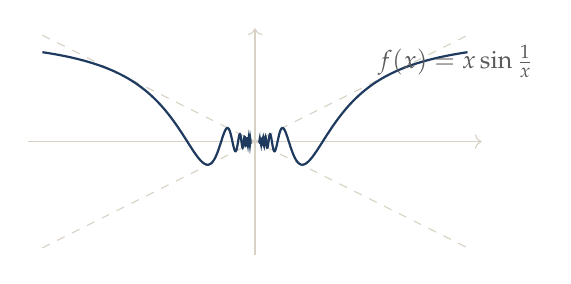
\begin{tikzpicture}[scale=0.9]
\draw[->,linie] (-3.2,0)--(3.2,0); \draw[->,linie] (0,-1.6)--(0,1.6);
\draw[linie,dashed] (-3,-1.5)--(3,1.5); \draw[linie,dashed] (-3,1.5)--(3,-1.5);
\draw[tief,thick,domain=0.06:3,samples=600,smooth] plot (\x,{0.5*\x*sin(deg(3/\x))});
\draw[tief,thick,domain=-3:-0.06,samples=600,smooth] plot (\x,{0.5*\x*sin(deg(3/\x))});
\node[grau,font=\small,anchor=north west] at (1.6,1.5) {$f(x) = x\sin\frac1x$};
\end{tikzpicture}
\end{center}
\probe{$f(0{,}001) = 0{,}001\cdot\sin(1000) = 0{,}001\cdot0{,}827 = 0{,}0008$ --- winzig. $g(0{,}001) = 0{,}827$, $g(0{,}0010005) = \sin(999{,}5) = -0{,}95$ --- springt. \checkmark}
\begin{mitnehmen}\kastentext
Unendlich viele Schwingungen sind kein Hindernis für Stetigkeit, solange ihre Amplitude gegen null geht. Das Einschließungsargument $|f(x)|\le|x|$ ist der Standardweg, Stetigkeit an einer kritischen Stelle zu zeigen; zwei Folgen mit verschiedenen Grenzwerten der Standardweg, sie zu widerlegen.
\end{mitnehmen}
\end{loesungkarte}

%%%%%%%%%% 3.19
\stupserzwei{gruen}{$p(x) = a_nx^{n}\bigl(1 + \frac{a_{n-1}}{a_nx} + \dots + \frac{a_0}{a_nx^{n}}\bigr)$; die Klammer geht gegen $1$ für $|x|\to\infty$.}{22pt}
\begin{loesungkarte}{gruen}{3.19}{Ungerader Grad, reelle Nullstelle}
\derweg{Für großes $|x|$ dominiert $a_nx^{n}$ und hat bei $\pm M$ verschiedene Vorzeichen; Zwischenwertsatz.}
\schritt{Normieren}
Ohne Einschränkung $a_n > 0$ (sonst betrachte $-p$). Schreibe $p(x) = x^{n}\,q(x)$ mit $q(x) = a_n + \frac{a_{n-1}}x + \dots + \frac{a_0}{x^{n}}$ für $x\neq0$. Es gilt $q(x)\to a_n > 0$ für $x\to\pm\infty$.
\schritt{Vorzeichen}
Also gibt es $M > 0$ mit $q(x) > 0$ für $|x|\ge M$. Dann ist $p(M) = M^{n}q(M) > 0$ und, weil $n$ ungerade ist, $p(-M) = (-M)^{n}q(-M) = -M^{n}q(-M) < 0$.
\schritt{Zwischenwertsatz}
$p$ ist stetig auf $[-M, M]$ und wechselt das Vorzeichen: Es gibt $\xi\in(-M, M)$ mit $p(\xi) = 0$. $\blacksquare$
\probe{$x^{3} - 2x + 5$: $p(-3) = -27 + 6 + 5 = -16$, $p(0) = 5$: Nullstelle in $(-3, 0)$, nämlich $\approx-2{,}09$. \checkmark\ Gegenbeispiel für geraden Grad: $x^{2} + 1$ hat keine reelle Nullstelle --- $p(\pm M) > 0$ auf beiden Seiten.}
\begin{mitnehmen}\kastentext
Das Argument ist rein qualitativ: Man weiß nichts über die Lage der Nullstelle, nur dass eine existiert. Für Polynome ergänzt der Fundamentalsatz der Algebra (Band 10): Über $\mathbb C$ hat \emph{jedes} nichtkonstante Polynom eine Nullstelle, und reelle Polynome ungeraden Grades haben eine ungerade Anzahl reeller.
\end{mitnehmen}
\end{loesungkarte}

%%%%%%%%%% 3.20
\stupserzwei{gruen}{O.\,B.\,d.\,A.\ $x\ge y$: $(\sqrt x - \sqrt y)^{2} = x - 2\sqrt{xy} + y\le x - y\iff2y\le2\sqrt{xy}\iff y\le\sqrt{xy}$, wahr wegen $x\ge y$.}{22pt}
\begin{loesungkarte}{gruen}{3.20}{Die Wurzel ist gleichmäßig stetig}
\derweg{Eine Ungleichung, die den Abstand der Wurzeln durch den Abstand der Zahlen kontrolliert --- unabhängig von der Stelle; dann $\delta$ aus ihr ablesen.}
\schritt{Die Ungleichung}
Behauptung: $|\sqrt x - \sqrt y|\le\sqrt{|x - y|}$ für $x, y\ge0$. Sei $x\ge y$. Beide Seiten sind $\ge0$, also darf man quadrieren: $(\sqrt x - \sqrt y)^{2} = x + y - 2\sqrt{xy}\le x - y\iff2y\le2\sqrt{xy}\iff\sqrt y\le\sqrt x$. Wahr. \checkmark
\schritt{$\delta$ wählen}
Sei $\varepsilon > 0$. Setze $\delta = \varepsilon^{2}$. Für alle $x, y\ge0$ mit $|x - y| < \delta$: $|\sqrt x - \sqrt y|\le\sqrt{|x - y|} < \sqrt\delta = \varepsilon$. $\blacksquare$ --- $\delta$ hängt nur von $\varepsilon$ ab, nicht von $x$ oder $y$: gleichmäßig.
\schritt{Warum das überrascht}
$f'(x) = \frac1{2\sqrt x}\to\infty$ für $x\to0$. Eine beschränkte Ableitung garantiert gleichmäßige Stetigkeit (Mittelwertsatz), aber sie ist nicht nötig: Die Wurzel ist bei $0$ steil, aber nur auf einem winzigen Stück --- der Zuwachs $\sqrt{\delta}$ bleibt klein.
\probe{$x = 0$, $y = 0{,}0001$: $|\sqrt x - \sqrt y| = 0{,}01 = \sqrt{0{,}0001}$ --- die Ungleichung ist hier scharf. $x = 100$, $y = 100{,}0001$: Abstand der Wurzeln $5\cdot10^{-6}$, weit unter $0{,}01$. \checkmark}
\begin{mitnehmen}\kastentext
Gleichmäßig stetig: ein $\delta$ für alle Stellen. Hinreichend sind: kompakter Definitionsbereich (Satz von Heine), beschränkte Ableitung (Lipschitz), oder eine Abschätzung $|f(x) - f(y)|\le\omega(|x - y|)$ mit $\omega(t)\to0$ --- hier $\omega(t) = \sqrt t$ (Hölder-Stetigkeit). $\frac1x$ auf $(0, 1)$ und $x^{2}$ auf $\mathbb R$ sind \emph{nicht} gleichmäßig stetig.
\end{mitnehmen}
\end{loesungkarte}

%%%%%%%%%% 3.21
\stupserzwei{tief}{(c) Durch $3^{x}$ teilen: $(\frac23)^{x} = 5$, logarithmieren: $x\ln\frac23 = \ln5$. Der Nenner ist negativ --- $x$ ist negativ.}{22pt}
\begin{loesungkarte}{tief}{3.21}{Gleichungen mit $e$ und $\ln$}
\derweg{Substituieren, zusammenfassen, logarithmieren --- und am Ende den Definitionsbereich prüfen.}
\schritt{(a)}
$u = e^{x} > 0$: $u^{2} - 3u + 2 = (u - 1)(u - 2) = 0$, $u = 1$ oder $u = 2$. Also $x = \ln1 = 0$ oder $x = \ln2\approx0{,}693$.
\schritt{(b)}
Definitionsbereich: $x > 0$ und $x > 3$, also $x > 3$. $\ln(x(x - 3)) = \ln4\Rightarrow x^{2} - 3x - 4 = 0\Rightarrow(x - 4)(x + 1) = 0$. $x = -1$ liegt außerhalb des Definitionsbereichs. Einzige Lösung $x = 4$.
\schritt{(c)}
$\bigl(\frac23\bigr)^{x} = 5\Rightarrow x\ln\frac23 = \ln5\Rightarrow x = \frac{\ln5}{\ln(2/3)} = \frac{1{,}6094}{-0{,}4055} = -3{,}969$. Plausibel: Für negatives $x$ wird $2^{x}$ \emph{größer} als $3^{x}$, und das muss es, um das Fünffache zu sein.
\schritt{(d)}
Setze $a = \ln x$, $b = \ln y$ (für $x, y > 0$). Dann $\exp(a + b) = \exp a\exp b = xy$, also $a + b = \ln(xy)$, das heißt $\ln x + \ln y = \ln(xy)$. $\blacksquare$ --- Die Funktionalgleichung der Exponentialfunktion \emph{ist} die des Logarithmus, gelesen von der anderen Seite.
\probe{(a) $e^{2\ln2} - 3e^{\ln2} + 2 = 4 - 6 + 2 = 0$. \checkmark\ (b) $\ln4 + \ln1 = \ln4$. \checkmark\ (c) $2^{-3{,}969} = 0{,}0638$, $5\cdot3^{-3{,}969} = 5\cdot0{,}01276 = 0{,}0638$. \checkmark}
\begin{mitnehmen}\kastentext
$a^{x} = e^{x\ln a}$ reduziert jede Exponentialfunktion auf $e^{x}$, und $\log_ab = \frac{\ln b}{\ln a}$ jeden Logarithmus auf $\ln$. Bei Logarithmusgleichungen entstehen durch das Zusammenfassen Scheinlösungen --- die Probe gehört zur Lösung.
\end{mitnehmen}
\end{loesungkarte}

%%%%%%%%%% 3.22
\stupserzwei{gruen}{Glieder: $1$; $-0{,}125$; $+0{,}0026042$; $-0{,}0000217$; $+0{,}0000001$. Das sechste Glied $\frac{0{,}5^{10}}{10!}\approx2{,}7\cdot10^{-10}$ ist die Fehlerschranke.}{22pt}
\begin{loesungkarte}{gruen}{3.22}{$\cos(0{,}5)$ auf vier Stellen}
\derweg{Reihe aufschreiben, Glieder berechnen, bis sie unter die Toleranz fallen; Leibniz-Restabschätzung.}
\schritt{Reihe}
$\cos x = \sum_{k\ge0}\frac{(-1)^{k}x^{2k}}{(2k)!} = 1 - \frac{x^{2}}2 + \frac{x^{4}}{24} - \frac{x^{6}}{720} + \frac{x^{8}}{40320} - \dots$
\schritt{Glieder für $x = 0{,}5$}
$1$; $\frac{0{,}25}2 = 0{,}125$; $\frac{0{,}0625}{24} = 0{,}00260417$; $\frac{0{,}015625}{720} = 0{,}00002170$; $\frac{0{,}00390625}{40320} = 0{,}00000010$.
\schritt{Summe}
$1 - 0{,}125 + 0{,}00260417 - 0{,}00002170 + 0{,}00000010 = 0{,}87758257$. Auf vier Stellen: $\cos(0{,}5)\approx0{,}8776$.
\schritt{Fehlerschranke}
Alternierende Reihe mit monoton fallenden Gliedern: Der Fehler nach $n$ Gliedern ist kleiner als das erste weggelassene. Nach den ersten drei Gliedern ($0{,}87760417$) ist der Fehler $< 2{,}2\cdot10^{-5}$ --- das reicht für vier Stellen schon. Nach fünf Gliedern ist der Fehler $< \frac{0{,}5^{10}}{10!} = 2{,}7\cdot10^{-10}$.
\probe{Taschenrechner: $\cos(0{,}5) = 0{,}8775825619$. Abweichung von unserer Fünf-Glieder-Summe: $3\cdot10^{-10}$, unter der Schranke. \checkmark}
\begin{mitnehmen}\kastentext
Für $|x|\le1$ konvergieren die Reihen von $\sin$, $\cos$, $e^{x}$ rasend schnell (Fakultäten im Nenner). Für größere $x$ reduziert man erst: $\cos(x + 2\pi) = \cos x$, $e^{x} = (e^{x/2})^{2}$. Die Leibniz-Schranke \enquote{Fehler $<$ erstes weggelassenes Glied} gilt nur für alternierende Reihen mit monoton fallenden Beträgen.
\end{mitnehmen}
\end{loesungkarte}

%%%%%%%%%% 3.23
\stupserzwei{tief}{(a) $(e^{x\ln x})' = e^{x\ln x}\cdot(x\ln x)' = x^{x}(\ln x + 1)$.}{22pt}
\begin{loesungkarte}{tief}{3.23}{Ableiten im Akkord}
\derweg{Kettenregel von außen nach innen; bei $x^{x}$ zuerst als Exponentialfunktion schreiben.}
\schritt{(a)}
$x^{x} = e^{x\ln x}$. Ableitung: $e^{x\ln x}\cdot(1\cdot\ln x + x\cdot\frac1x) = x^{x}(\ln x + 1)$. Nullstelle bei $x = \frac1e$: dort hat $x^{x}$ sein Minimum $e^{-1/e}\approx0{,}692$.
\schritt{(b)}
$(\ln(\cos x))' = \frac1{\cos x}\cdot(-\sin x) = -\tan x$.
\schritt{(c)}
$(\arctan(2x))' = \frac1{1 + (2x)^{2}}\cdot2 = \frac2{1 + 4x^{2}}$.
\schritt{(d)}
$(\sin^{2}(3x))' = 2\sin(3x)\cdot\cos(3x)\cdot3 = 6\sin(3x)\cos(3x) = 3\sin(6x)$.
\schritt{(e)}
$(xe^{-x^{2}})' = e^{-x^{2}} + x\cdot e^{-x^{2}}\cdot(-2x) = e^{-x^{2}}(1 - 2x^{2})$. Extrema bei $x = \pm\frac1{\sqrt2}$.
\probe{(a) numerisch bei $x = 2$: $\frac{2{,}001^{2{,}001} - 2^{2}}{0{,}001} = \frac{4{,}00677 - 4}{0{,}001} = 6{,}77$; Formel: $4(\ln2 + 1) = 6{,}77$. \checkmark\ (d) bei $x = 0{,}1$: $3\sin0{,}6 = 1{,}694$; $6\sin0{,}3\cos0{,}3 = 6\cdot0{,}2955\cdot0{,}9553 = 1{,}694$. \checkmark}
\begin{mitnehmen}\kastentext
Zwei Umschreibungen, die man automatisch macht: $f(x)^{g(x)} = e^{g(x)\ln f(x)}$ und $\log_a x = \frac{\ln x}{\ln a}$. Dann bleiben nur noch $e^{x}$, $\ln$, Potenzen, $\sin$, $\cos$, $\arctan$ --- und die drei Regeln.
\end{mitnehmen}
\end{loesungkarte}

%%%%%%%%%% 3.24
\stupserzwei{akzent}{(c) $f(x) - f(a) = \frac{f(x) - f(a)}{x - a}\cdot(x - a)\to f'(a)\cdot0 = 0$.}{22pt}
\begin{loesungkarte}{akzent}{3.24}{Stetig, aber nicht differenzierbar}
\derweg{Differenzenquotient von beiden Seiten; der Beweis der Implikation ist ein Einzeiler mit Grenzwertsätzen.}
\schritt{(a)}
Stetig: $||x| - 0|= |x|\to0$. Differenzenquotient in $0$: $\frac{|h| - 0}h = \frac{|h|}h$, das ist $1$ für $h > 0$ und $-1$ für $h < 0$. Rechts- und linksseitiger Grenzwert verschieden: nicht differenzierbar. Ein Knick.
\schritt{(b)}
Stetig: $\sqrt[3]h\to0$. Differenzenquotient: $\frac{\sqrt[3]h - 0}h = h^{-2/3}\to+\infty$ für $h\to0$ (von beiden Seiten). Nicht differenzierbar --- aber anders als bei $|x|$: Hier gibt es \emph{eine} Grenzrichtung, nur ist die Steigung unendlich. Eine senkrechte Tangente.
\schritt{(c)}
Für $x\neq a$: $f(x) - f(a) = \frac{f(x) - f(a)}{x - a}\cdot(x - a)$. Für $x\to a$ geht der erste Faktor gegen $f'(a)$ (existiert nach Voraussetzung), der zweite gegen $0$; das Produkt gegen $0$. Also $f(x)\to f(a)$: stetig. $\blacksquare$
\schritt{(d)}
$(x\cdot x)' = (x^{2})' = 2x$, aber $f'g' = 1\cdot1 = 1$. Richtig: $(fg)' = f'g + fg'$, hier $1\cdot x + x\cdot1 = 2x$. \checkmark
\begin{fehler}\kastentext
Differenzierbar $\Rightarrow$ stetig, nie umgekehrt. Stetige Funktionen können Knicke haben ($|x|$), senkrechte Tangenten ($\sqrt[3]x$) oder --- wie die Weierstraß-Funktion --- \emph{nirgends} differenzierbar sein. Und $(fg)' = f'g'$ ist der häufigste Ableitungsfehler überhaupt; die Probe $(x\cdot x)'$ entlarvt ihn in einer Zeile.
\end{fehler}
\begin{mitnehmen}\kastentext
Differenzierbar heißt: Der Differenzenquotient hat einen Grenzwert, \emph{eine} Zahl, von beiden Seiten dieselbe und endlich. Jede dieser drei Bedingungen kann einzeln scheitern.
\end{mitnehmen}
\end{loesungkarte}

%%%%%%%%%% 3.25
\stupserzwei{gruen}{$u = e^{x^{2}}\sin3x$, $u' = 2xe^{x^{2}}\sin3x + 3e^{x^{2}}\cos3x$. Dann $f' = \frac{u'(1 + x^{2}) - u\cdot2x}{(1 + x^{2})^{2}}$.}{22pt}
\begin{loesungkarte}{gruen}{3.25}{Alle drei Regeln auf einmal}
\derweg{Zähler als Produkt ableiten (mit Kettenregel in jedem Faktor), dann Quotientenregel, dann ausklammern.}
\schritt{Zähler}
$u(x) = e^{x^{2}}\sin(3x)$. $(e^{x^{2}})' = 2xe^{x^{2}}$, $(\sin3x)' = 3\cos3x$. Produktregel: $u' = 2xe^{x^{2}}\sin3x + 3e^{x^{2}}\cos3x = e^{x^{2}}(2x\sin3x + 3\cos3x)$.
\schritt{Quotient}
$f' = \frac{u'(1 + x^{2}) - 2xu}{(1 + x^{2})^{2}} = \frac{e^{x^{2}}\bigl[(2x\sin3x + 3\cos3x)(1 + x^{2}) - 2x\sin3x\bigr]}{(1 + x^{2})^{2}}$.
\schritt{Vereinfachen}
In der Klammer: $2x\sin3x + 2x^{3}\sin3x + 3\cos3x + 3x^{2}\cos3x - 2x\sin3x = 2x^{3}\sin3x + 3(1 + x^{2})\cos3x$. Also
\[ f'(x) = \frac{e^{x^{2}}\bigl[2x^{3}\sin3x + 3(1 + x^{2})\cos3x\bigr]}{(1 + x^{2})^{2}}. \]
\probe{$x = 0$: $f'(0) = \frac{1\cdot[0 + 3\cdot1\cdot1]}1 = 3$. Direkt: nahe $0$ ist $f(x)\approx\sin3x\approx3x$, Steigung $3$. \checkmark}
\begin{mitnehmen}\kastentext
Bei verschachtelten Ausdrücken: Struktur erkennen (Quotient von Produkt von Verkettungen), von außen nach innen die Regeln anwenden, Teilergebnisse benennen ($u$, $u'$), und erst ganz am Ende vereinfachen. Wer unterwegs vereinfacht, verliert Terme.
\end{mitnehmen}
\end{loesungkarte}

%%%%%%%%%% 3.26
\stupserzwei{gruen}{$f'(x) = 2x\sin\frac1x - \cos\frac1x$ für $x\neq0$. Der erste Summand geht gegen $0$, der zweite schwingt zwischen $-1$ und $1$.}{22pt}
\begin{loesungkarte}{gruen}{3.26}{Differenzierbar mit unstetiger Ableitung}
\derweg{In $0$ direkt mit dem Differenzenquotienten; für $x\neq0$ mit den Regeln; dann $\lim_{x\to0}f'(x)$ untersuchen.}
\schritt{Differenzierbar in $0$}
$\frac{f(h) - f(0)}h = \frac{h^{2}\sin(1/h)}h = h\sin\frac1h$, und $|h\sin\frac1h|\le|h|\to0$. Also $f'(0) = 0$ existiert.
\schritt{$f'$ für $x\neq0$}
Produkt- und Kettenregel: $f'(x) = 2x\sin\frac1x + x^{2}\cos\frac1x\cdot\bigl(-\frac1{x^{2}}\bigr) = 2x\sin\frac1x - \cos\frac1x$.
\schritt{$f'$ ist in $0$ nicht stetig}
$2x\sin\frac1x\to0$, aber $\cos\frac1x$ hat für $x\to0$ keinen Grenzwert (bei $x_n = \frac1{2n\pi}$ ist er $1$, bei $y_n = \frac1{(2n + 1)\pi}$ ist er $-1$). Also existiert $\lim_{x\to0}f'(x)$ nicht, und $f'$ ist in $0$ unstetig --- obwohl $f'(0) = 0$ definiert ist.
\probe{$x = 0{,}01$: $f'(0{,}01) = 0{,}02\sin100 - \cos100 = 0{,}02\cdot(-0{,}506) - 0{,}862 = -0{,}872$. $x = 0{,}0101$: $\cos(99{,}01) = 0{,}124$, $f'\approx-0{,}13$. Große Sprünge auf kleinem Raum. \checkmark}
\begin{mitnehmen}\kastentext
\enquote{$f$ differenzierbar} und \enquote{$f'$ stetig} ($f\in C^{1}$) sind verschiedene Eigenschaften. Der Faktor $x^{2}$ ist genau das Maß an Dämpfung, das Differenzierbarkeit in $0$ erzwingt, aber die Ableitung noch wild lässt; $x^{3}\sin\frac1x$ wäre $C^{1}$.
\end{mitnehmen}
\end{loesungkarte}

%%%%%%%%%% 3.27
\stupserzwei{tief}{(d) $\frac d{dx}\arctan\frac1x = \frac1{1 + 1/x^{2}}\cdot\bigl(-\frac1{x^{2}}\bigr) = -\frac1{x^{2} + 1}$. Die Summe der Ableitungen ist null.}{22pt}
\begin{loesungkarte}{tief}{3.27}{Ungleichungen mit dem Mittelwertsatz}
\derweg{Differenzfunktion bilden; an einer Stelle gleich null; Ableitung hat festes Vorzeichen, also ist die Differenz monoton.}
\schritt{(a)}
$g(x) = e^{x} - 1 - x$, $g(0) = 0$, $g'(x) = e^{x} - 1$: negativ für $x < 0$, positiv für $x > 0$. Also fällt $g$ bis $0$ und steigt danach: $g(x)\ge g(0) = 0$ überall. $\blacksquare$
\schritt{(b)}
$h(x) = x - \sin x$, $h(0) = 0$, $h'(x) = 1 - \cos x\ge0$. $h$ ist monoton wachsend, also $h(x)\ge0$ für $x\ge0$. $\blacksquare$
\schritt{(c)}
$k(x) = x - \ln(1 + x)$ auf $(-1, \infty)$, $k(0) = 0$, $k'(x) = 1 - \frac1{1 + x} = \frac x{1 + x}$: negativ auf $(-1, 0)$, positiv auf $(0, \infty)$. Minimum bei $0$: $k\ge0$. $\blacksquare$
\schritt{(d)}
$F(x) = \arctan x + \arctan\frac1x$ auf $(0, \infty)$. $F'(x) = \frac1{1 + x^{2}} + \frac1{1 + 1/x^{2}}\cdot\bigl(-\frac1{x^{2}}\bigr) = \frac1{1 + x^{2}} - \frac1{x^{2} + 1} = 0$. Nach dem Mittelwertsatz ist $F$ auf dem Intervall konstant; $F(1) = \frac\pi4 + \frac\pi4 = \frac\pi2$. $\blacksquare$
\probe{(a) $x = 1$: $e\ge2$. \checkmark\ $x = -2$: $e^{-2} = 0{,}135\ge-1$. \checkmark\ (d) $x = \sqrt3$: $\frac\pi3 + \frac\pi6 = \frac\pi2$. \checkmark}
\begin{mitnehmen}\kastentext
Der Mittelwertsatz in zwei Folgerungen: $g'\ge0\Rightarrow g$ monoton wachsend; $g' = 0\Rightarrow g$ konstant. Mit der ersten beweist man Ungleichungen (Differenz bilden, Nullstelle, Vorzeichen der Ableitung), mit der zweiten Identitäten (Ableitung null, Wert an einer Stelle). Beide brauchen ein \emph{Intervall}: Auf $(-\infty, 0)$ ist $F$ in (d) ebenfalls konstant, aber gleich $-\frac\pi2$.
\end{mitnehmen}
\end{loesungkarte}

%%%%%%%%%% 3.28
\stupserzwei{akzent}{(b) $\frac{x + \sin x}x = 1 + \frac{\sin x}x\to1 + 0 = 1$, denn $|\sin x|\le1$. Der Grenzwert existiert --- L'Hospital hat ihn nur nicht gefunden.}{22pt}
\begin{loesungkarte}{akzent}{3.28}{L'Hospital, falsch angewandt}
\derweg{In jedem Fall prüfen, welche Voraussetzung fehlt; dann die Regel mit allen Bedingungen aufschreiben.}
\schritt{(a) keine unbestimmte Form}
Einsetzen: $\frac{1 + 1}{1 + 1} = 1$. Die Funktion ist in $1$ stetig, der Grenzwert ist der Funktionswert. L'Hospital setzt $\frac00$ oder $\frac\infty\infty$ voraus; hier liegt $\frac22$ vor, und die Regel liefert Unsinn ($2$ statt $1$).
\schritt{(b) Ableitungsquotient ohne Grenzwert}
$\frac\infty\infty$ liegt vor. Aber $\frac{(x + \sin x)'}{x'} = 1 + \cos x$ hat für $x\to\infty$ keinen Grenzwert. Die Regel sagt dann \emph{nichts} --- nicht, dass der ursprüngliche Grenzwert fehlt. Er existiert: $1 + \frac{\sin x}x\to1$. L'Hospital ist eine Einbahnstraße: Existiert der Grenzwert der Ableitungen, dann auch der ursprüngliche und beide sind gleich. Umgekehrt nicht.
\schritt{(c) Zirkelschluss}
$\frac{\sin x}x\to\frac{\cos0}1 = 1$ ist formal korrekt --- wenn man $(\sin x)' = \cos x$ schon hat. Leitet man aber $\sin$ über den Differenzenquotienten ab, braucht man gerade $\lim\frac{\sin h}h = 1$. Dann beweist das Argument die Aussage mit sich selbst. In Band 3 ist $\sin$ über die Potenzreihe definiert, dort ist $(\sin)' = \cos$ unabhängig --- und L'Hospital hier erlaubt, wenn auch mit Kanonen auf Spatzen.
\schritt{(d) die Regel}
Seien $f, g$ auf $(a, b)$ differenzierbar, $g'\neq0$ dort, und entweder $f, g\to0$ oder $|g|\to\infty$ für $x\to a^{+}$. \emph{Existiert} $\lim_{x\to a^{+}}\frac{f'(x)}{g'(x)} = L$ (auch $\pm\infty$ zugelassen), dann ist $\lim_{x\to a^{+}}\frac{f(x)}{g(x)} = L$. Entsprechend für $x\to b^{-}$, $x\to\pm\infty$.
\begin{fehler}\kastentext
Drei Prüfungen vor jeder Anwendung: (1) Liegt $\frac00$ oder $\frac\infty\infty$ vor? (2) Existiert der Grenzwert des Ableitungsquotienten? (3) Benutze ich etwas, das ich erst beweisen will? Und eine Alternative immer im Blick: Oft sind Umformen (Aufgabe 3.4) oder Taylorreihen (Aufgabe 3.31) schneller und sicherer.
\end{fehler}
\begin{mitnehmen}\kastentext
L'Hospital ist ein Werkzeug für $\frac00$ und $\frac\infty\infty$, nichts sonst; $0\cdot\infty$, $\infty - \infty$, $1^{\infty}$ muss man erst umschreiben. Und wenn das Ableiten den Ausdruck nicht vereinfacht, ist die Regel das falsche Werkzeug.
\end{mitnehmen}
\end{loesungkarte}

%%%%%%%%%% 3.29
\stupserzwei{gruen}{(b) $\frac{\ln x}{1/x}$ ist $\frac{-\infty}\infty$; Ableitungen: $\frac{1/x}{-1/x^{2}} = -x\to0$.}{22pt}
\begin{loesungkarte}{gruen}{3.29}{Drei Grenzwerte mit L'Hospital}
\derweg{Form prüfen, gegebenenfalls umschreiben, ableiten, Grenzwert der Ableitungen bestimmen.}
\schritt{(a)}
$\frac00$. Erste Anwendung: $\frac{e^{x} - 1}{2x}$, wieder $\frac00$. Zweite: $\frac{e^{x}}2\to\frac12$. Also $\lim = \frac12$.
\schritt{(b)}
$0\cdot(-\infty)$; umschreiben $x\ln x = \frac{\ln x}{1/x}$, Form $\frac{-\infty}{\infty}$. Ableiten: $\frac{1/x}{-1/x^{2}} = -x\to0$. Also $\lim_{x\to0^{+}}x\ln x = 0$.
\schritt{(c)}
$0^{0}$; $x^{x} = e^{x\ln x}$, und $x\ln x\to0$ nach (b). Da $\exp$ stetig: $x^{x}\to e^{0} = 1$.
\probe{(a) $x = 0{,}01$: $\frac{e^{0{,}01} - 1{,}01}{0{,}0001} = \frac{0{,}00005017}{0{,}0001} = 0{,}5017$. \checkmark\ (c) $0{,}01^{0{,}01} = e^{0{,}01\ln0{,}01} = e^{-0{,}046} = 0{,}955$; $0{,}001^{0{,}001} = 0{,}993$. \checkmark}
\begin{mitnehmen}\kastentext
(a) sagt: $e^{x} = 1 + x + \frac{x^{2}}2 + \dots$, der Fehler der linearen Näherung ist $\sim\frac{x^{2}}2$. (b) sagt: $\ln x$ geht gegen $-\infty$, aber langsamer als jede Potenz von $x$ gegen $0$ geht. (c) ist die Rechtfertigung für $0^{0} = 1$ in Potenzreihen --- als Grenzwert von $x^{x}$, nicht als allgemeine Regel.
\end{mitnehmen}
\end{loesungkarte}

%%%%%%%%%% 3.30
\stupserzwei{gruen}{$f' = -\frac{2x}{(x^{2} - 1)^{2}}$: Vorzeichen von $-x$. $f'' = \frac{6x^{2} + 2}{(x^{2} - 1)^{3}}$: Vorzeichen von $x^{2} - 1$.}{22pt}
\begin{loesungkarte}{gruen}{3.30}{Eine Kurvendiskussion}
\derweg{Das Programm der Reihe nach; die Umschreibung $f = 1 + \frac1{x^{2} - 1}$ macht alles schneller.}
\schritt{Definitionsbereich, Symmetrie}
$D = \mathbb R\setminus\{-1, 1\}$. $f(-x) = f(x)$: gerade, achsensymmetrisch zur $y$-Achse.
\schritt{Nullstellen, Pole}
$f(x) = 0\iff x = 0$. Pole bei $x = \pm1$: Für $x\to1^{+}$ ist $x^{2} - 1\to0^{+}$, also $f\to+\infty$; für $x\to1^{-}$: $f\to-\infty$. Spiegelbildlich bei $-1$.
\schritt{Asymptote}
$f(x) = 1 + \frac1{x^{2} - 1}\to1$ für $x\to\pm\infty$; von oben ($\frac1{x^{2} - 1} > 0$ für $|x| > 1$). Waagerechte Asymptote $y = 1$.
\schritt{Monotonie, Extrema}
$f'(x) = -\frac{2x}{(x^{2} - 1)^{2}}$. $f' > 0$ für $x < 0$ (außer $-1$), $f' < 0$ für $x > 0$ (außer $1$). Kritischer Punkt $x = 0$: lokales Maximum $f(0) = 0$. Auf $(-1, 1)$ ist $f\le0$, auf $|x| > 1$ ist $f > 1$: Die Werte in $(0, 1]$ werden nie angenommen.
\schritt{Krümmung}
$f''(x) = \frac{6x^{2} + 2}{(x^{2} - 1)^{3}}$. Zähler $> 0$; Nenner $> 0$ für $|x| > 1$ (konvex), $< 0$ für $|x| < 1$ (konkav). Keine Wendepunkte ($f''\neq0$; der Krümmungswechsel passiert an den Polen).
\begin{center}
\begin{tikzpicture}[scale=0.85]
\draw[->,linie] (-3.5,0)--(3.5,0) node[right,grau,font=\small] {$x$};
\draw[->,linie] (0,-3)--(0,3.4) node[above,grau,font=\small] {$y$};
\draw[linie,dashed] (-3.5,1)--(3.5,1); \draw[linie,dashed] (1,-3)--(1,3.4); \draw[linie,dashed] (-1,-3)--(-1,3.4);
\draw[tief,thick,domain=1.18:3.5,samples=100,smooth] plot (\x,{\x*\x/(\x*\x-1)});
\draw[tief,thick,domain=-3.5:-1.18,samples=100,smooth] plot (\x,{\x*\x/(\x*\x-1)});
\draw[tief,thick,domain=-0.82:0.82,samples=100,smooth] plot (\x,{\x*\x/(\x*\x-1)});
\node[grau,font=\small,anchor=west] at (2.2,1.35) {$y = 1$};
\fill[akzent] (0,0) circle (1.6pt);
\end{tikzpicture}
\end{center}
\probe{$f(2) = \frac43 = 1{,}33$, $f(0{,}5) = \frac{0{,}25}{-0{,}75} = -\frac13$, $f(1{,}1) = \frac{1{,}21}{0{,}21} = 5{,}76$. Passt zur Skizze. \checkmark\ $f''(2) = \frac{26}{27} > 0$ konvex; $f''(0) = \frac2{-1} = -2 < 0$ konkav, Maximum. \checkmark}
\begin{mitnehmen}\kastentext
Bei gebrochen rationalen Funktionen zuerst Polynomdivision: $f = 1 + \frac1{x^{2} - 1}$ zeigt Asymptote und Vorzeichenverhalten ohne Rechnung. Dann das Programm --- aber mit Verstand: Symmetrie halbiert die Arbeit, und wer die Pole kennt, weiß schon, wo die Krümmung wechselt.
\end{mitnehmen}
\end{loesungkarte}

%%%%%%%%%% 3.31
\stupserzwei{tief}{(b) $(1 + x + \frac{x^{2}}2 + \frac{x^{3}}6)(x - \frac{x^{3}}6)$: $x^{1}$: $x$; $x^{2}$: $x^{2}$; $x^{3}$: $\frac{x^{3}}2 - \frac{x^{3}}6 = \frac{x^{3}}3$.}{22pt}
\begin{loesungkarte}{tief}{3.31}{Rechnen mit Taylorreihen}
\derweg{Reihen einsetzen, niedrigste Potenzen sammeln, kürzen; Fehler mit dem Lagrange-Restglied.}
\schritt{(a)}
$\cos x - 1 + \frac{x^{2}}2 = \frac{x^{4}}{24} - \frac{x^{6}}{720} + \dots$, geteilt durch $x^{4}$: $\frac1{24} - \frac{x^{2}}{720} + \dots\to\frac1{24}$. \\
$\sin x - x = -\frac{x^{3}}6 + \frac{x^{5}}{120} - \dots$, geteilt durch $x^{3}$: $\to-\frac16$.
\schritt{(b)}
$e^{x}\sin x = \bigl(1 + x + \frac{x^{2}}2 + \frac{x^{3}}6 + \dots\bigr)\bigl(x - \frac{x^{3}}6 + \dots\bigr)$. Koeffizienten: $x$: $1$; $x^{2}$: $1$; $x^{3}$: $\frac12 - \frac16 = \frac13$. Also $T_3(x) = x + x^{2} + \frac{x^{3}}3$.
\schritt{(c)}
Restglied nach dem Glied $-\frac{x^{3}}6$ (das $x^{4}$-Glied ist null): $R = \frac{\sin^{(5)}(\xi)}{5!}x^{5} = \frac{\cos\xi}{120}x^{5}$, also $|R|\le\frac{|x|^{5}}{120}\le\frac{0{,}5^{5}}{120} = \frac{0{,}03125}{120} = 2{,}6\cdot10^{-4}$. (Leibniz-Abschätzung mit dem nächsten Glied $\frac{x^{5}}{120}$ liefert dasselbe.)
\probe{(a) $x = 0{,}1$: $\frac{\cos0{,}1 - 1 + 0{,}005}{10^{-4}} = \frac{4{,}1653\cdot10^{-6}}{10^{-4}} = 0{,}04165\approx\frac1{24} = 0{,}04167$. \checkmark\ (b) $x = 0{,}1$: $e^{0{,}1}\sin0{,}1 = 0{,}110332$; $T_3 = 0{,}1 + 0{,}01 + 0{,}000333 = 0{,}110333$. \checkmark\ (c) $\sin0{,}5 = 0{,}479426$; $0{,}5 - \frac{0{,}125}6 = 0{,}479167$; Fehler $2{,}6\cdot10^{-4}$. \checkmark}
\begin{mitnehmen}\kastentext
Für Grenzwerte bei $0$ sind Taylorreihen oft schneller als L'Hospital: Man sieht sofort, welche Potenz übrig bleibt. Die drei Reihen $e^{x}$, $\sin x$, $\cos x$ und dazu $\frac1{1 - x}$, $\ln(1 + x)$ sollte man bis zur vierten Potenz auswendig können.
\end{mitnehmen}
\end{loesungkarte}

%%%%%%%%%% 3.32
\stupserzwei{gruen}{$T_2(x) = 1 + \frac12(x - 1) - \frac18(x - 1)^{2}$; bei $x = 1{,}1$: $1 + 0{,}05 - 0{,}00125$.}{22pt}
\begin{loesungkarte}{gruen}{3.32}{$\sqrt{1{,}1}$ mit Fehlerschranke}
\derweg{Entwickeln um $x_0 = 1$, wo alles exakt ist; Lagrange-Restglied mit der dritten Ableitung.}
\schritt{Ableitungen bei $1$}
$f(x) = x^{1/2}$, $f(1) = 1$; $f' = \frac12x^{-1/2}$, $f'(1) = \frac12$; $f'' = -\frac14x^{-3/2}$, $f''(1) = -\frac14$; $f''' = \frac38x^{-5/2}$.
\schritt{Taylorpolynom}
$T_2(x) = 1 + \frac12(x - 1) - \frac18(x - 1)^{2}$. Bei $x = 1{,}1$: $1 + 0{,}05 - 0{,}00125 = 1{,}04875$.
\schritt{Restglied}
$R_2 = \frac{f'''(\xi)}{3!}(0{,}1)^{3}$ mit $\xi\in(1, 1{,}1)$. Dort $f'''(\xi) = \frac38\xi^{-5/2}\le\frac38$. Also $|R_2|\le\frac{3/8}6\cdot0{,}001 = 6{,}25\cdot10^{-5}$. Garantiert: $\sqrt{1{,}1}\in[1{,}04869;\ 1{,}04881]$. Da $f''' > 0$, ist $R_2 > 0$: der wahre Wert liegt über $1{,}04875$.
\probe{$\sqrt{1{,}1} = 1{,}0488088$; Fehler $5{,}9\cdot10^{-5} < 6{,}25\cdot10^{-5}$, positiv. \checkmark\ Gegenprobe: $1{,}04875^{2} = 1{,}09988$. \checkmark}
\begin{mitnehmen}\kastentext
Lagrange-Restglied: $R_n = \frac{f^{(n+1)}(\xi)}{(n + 1)!}(x - x_0)^{n+1}$ mit unbekanntem $\xi$ zwischen $x_0$ und $x$; man schätzt $|f^{(n+1)}|$ auf dem Intervall nach oben ab. Das Vorzeichen von $f^{(n+1)}$ verrät sogar die Richtung des Fehlers.
\end{mitnehmen}
\end{loesungkarte}

%%%%%%%%%% 3.33
\stupserzwei{gruen}{Oder: $\frac1{1 + x} = \sum(-x)^{k}$ gliedweise integrieren von $0$ bis $x$.}{22pt}
\begin{loesungkarte}{gruen}{3.33}{Die Reihe von $\ln(1 + x)$}
\derweg{Ableitungen bei $0$, Muster erkennen, Konvergenzradius, beide Randpunkte prüfen.}
\schritt{Ableitungen}
$f = \ln(1 + x)$, $f(0) = 0$; $f' = (1 + x)^{-1}$, $f'(0) = 1$; $f'' = -(1 + x)^{-2}$, $f''(0) = -1$; $f''' = 2(1 + x)^{-3}$, $f'''(0) = 2$; $f^{(4)}(0) = -6$. Allgemein $f^{(k)}(0) = (-1)^{k+1}(k - 1)!$.
\schritt{Reihe}
$\frac{f^{(k)}(0)}{k!} = \frac{(-1)^{k+1}}k$, also
\[ \ln(1 + x) = \sum_{k\ge1}\frac{(-1)^{k+1}}kx^{k} = x - \frac{x^{2}}2 + \frac{x^{3}}3 - \frac{x^{4}}4 + \dots \]
Kürzer: $\frac1{1 + x} = \sum_{k\ge0}(-1)^{k}x^{k}$ für $|x| < 1$, gliedweise integriert von $0$ bis $x$ gibt dieselbe Reihe.
\schritt{Konvergenzbereich}
$R = \lim\frac{k + 1}k = 1$. Bei $x = 1$: $\sum\frac{(-1)^{k+1}}k$, Leibniz, konvergent. Bei $x = -1$: $\sum\frac{(-1)^{k+1}(-1)^{k}}k = -\sum\frac1k$, divergent (passend: $\ln0$ existiert nicht). Konvergenzbereich $(-1, 1]$.
\schritt{$\ln2$}
Bei $x = 1$ (Abelscher Grenzwertsatz rechtfertigt das Einsetzen am Rand): $\ln2 = 1 - \frac12 + \frac13 - \frac14 + \dots$
\probe{Partialsummen: $s_4 = 0{,}583$, $s_{10} = 0{,}646$, $s_{100} = 0{,}688$, $\ln2 = 0{,}693$. Konvergiert --- quälend langsam (Fehler $\approx\frac1{2n}$). \checkmark\ Schneller: $\ln2 = -\ln\frac12 = \sum\frac1{k2^{k}} = 0{,}5 + 0{,}125 + 0{,}0417 + 0{,}0156 + 0{,}0063 + \dots$, nach $10$ Gliedern $0{,}6930$. \checkmark}
\begin{mitnehmen}\kastentext
Zwei Wege zu Taylorreihen: Ableitungen berechnen (immer möglich, oft mühsam) oder bekannte Reihen umbauen --- integrieren, ableiten, substituieren (schnell, braucht die Sätze aus Kapitel 12). Das Randverhalten muss man immer gesondert prüfen; hier liefert es die berühmteste langsame Reihe der Analysis.
\end{mitnehmen}
\end{loesungkarte}

%%%%%%%%%% 3.34
\stupserzwei{tief}{(c) $\frac n{n^{2} + k^{2}} = \frac1n\cdot\frac1{1 + (k/n)^{2}}$: Riemann-Summe von $\frac1{1 + x^{2}}$.}{22pt}
\begin{loesungkarte}{tief}{3.34}{Summen, die Integrale sind}
\derweg{Den Faktor $\frac1n$ herausziehen, den Rest als $g(k/n)$ erkennen, dann $\int_0^1g$.}
\schritt{Prinzip}
Für stetiges $g$ auf $[0, 1]$ gilt $\frac1n\sum_{k=1}^{n}g\bigl(\frac kn\bigr)\to\int_0^1g(x)\,dx$ --- die rechte Riemann-Summe zur äquidistanten Zerlegung.
\schritt{(a)}
$\sum_{k=1}^{n}\frac1{n + k} = \frac1n\sum_{k=1}^{n}\frac1{1 + k/n}$, also $g(x) = \frac1{1 + x}$: Grenzwert $\int_0^1\frac{dx}{1 + x} = \ln2$.
\schritt{(b)}
$g(x) = x^{2}$: $\int_0^1x^{2}\,dx = \frac13$ (Aufgabe 3.35 beweist genau das).
\schritt{(c)}
$\frac n{n^{2} + k^{2}} = \frac1n\cdot\frac1{1 + (k/n)^{2}}$, $g(x) = \frac1{1 + x^{2}}$: $\int_0^1\frac{dx}{1 + x^{2}} = \arctan1 = \frac\pi4$.
\probe{(a) $n = 1000$: $0{,}69290$, $\ln2 = 0{,}69315$. \checkmark\ (c) $n = 1000$: $0{,}78515$, $\frac\pi4 = 0{,}78540$. \checkmark\ Der Fehler ist jeweils $\approx\frac c n$, wie bei Riemann-Summen üblich.}
\begin{mitnehmen}\kastentext
Rückwärts gelesen definiert die Riemann-Summe den Grenzwert von Summen, die keine geschlossene Form haben. (a) ist zugleich der Grund, warum $a_{2n} - a_n\to\ln2$ für die harmonische Reihe (Aufgabe 3.9 zeigte $\ge\frac12$) --- und der Anfang der Formel $a_n\approx\ln n + \gamma$.
\end{mitnehmen}
\end{loesungkarte}

%%%%%%%%%% 3.35
\stupserzwei{gruen}{$U_n = \frac{(n - 1)n(2n - 1)}{6n^{3}}$, $O_n = \frac{n(n + 1)(2n + 1)}{6n^{3}}$; beide gegen $\frac26 = \frac13$.}{22pt}
\begin{loesungkarte}{gruen}{3.35}{$\int_0^1x^{2}\,dx$ von Hand}
\derweg{Äquidistante Zerlegung, Infimum und Supremum auf jedem Teilintervall (Monotonie), Summenformel, Grenzwert.}
\schritt{Zerlegung}
$x_i = \frac in$, $i = 0, \dots, n$, Breite $\frac1n$. Auf $[x_{i-1}, x_i]$ ist $x^{2}$ monoton wachsend: $m_i = \bigl(\frac{i - 1}n\bigr)^{2}$, $M_i = \bigl(\frac in\bigr)^{2}$.
\schritt{Ober- und Untersumme}
$O_n = \sum_{i=1}^{n}\frac1n\Bigl(\frac in\Bigr)^{2} = \frac1{n^{3}}\sum_{i=1}^{n}i^{2} = \frac{n(n + 1)(2n + 1)}{6n^{3}}$, \quad $U_n = \frac1{n^{3}}\sum_{i=0}^{n-1}i^{2} = \frac{(n - 1)n(2n - 1)}{6n^{3}}$.
\schritt{Grenzwert}
$O_n = \frac16\bigl(1 + \frac1n\bigr)\bigl(2 + \frac1n\bigr)\to\frac26 = \frac13$, $U_n = \frac16\bigl(1 - \frac1n\bigr)\bigl(2 - \frac1n\bigr)\to\frac13$. Da $U_n\le\int\le O_n$ und beide gegen $\frac13$ gehen: $\int_0^1x^{2}\,dx = \frac13$. Außerdem $O_n - U_n = \frac1n\to0$: $x^{2}$ ist Riemann-integrierbar.
\probe{$n = 10$: $U = \frac{9\cdot10\cdot19}{6000} = 0{,}285$, $O = \frac{10\cdot11\cdot21}{6000} = 0{,}385$; Mittel $0{,}335\approx\frac13$. \checkmark\ Hauptsatz: $\bigl[\frac{x^{3}}3\bigr]_0^1 = \frac13$. \checkmark}
\begin{mitnehmen}\kastentext
So rechnete Archimedes (für die Parabel) und so definiert Riemann das Integral. Der Hauptsatz macht die Rechnung überflüssig --- aber nur, weil jemand sie einmal für $x^{n}$ gemacht hat. Bei monotonen Funktionen ist $O_n - U_n = \frac{f(b) - f(a)}n$, deshalb sind monotone Funktionen immer integrierbar.
\end{mitnehmen}
\end{loesungkarte}

%%%%%%%%%% 3.36
\stupserzwei{tief}{(e) $\sin^{2}x = \frac{1 - \cos2x}2$. (f) zweimal partiell, jedes Mal wird der Grad des Polynoms kleiner.}{22pt}
\begin{loesungkarte}{tief}{3.36}{Sechs Integrale, sechs Handgriffe}
\derweg{Muster erkennen: innere Ableitung als Faktor, $\frac{f'}f$, $\arctan$-Form, Doppelwinkel, partiell.}
\schritt{(a)}
$u = 1 + x^{2}$, $du = 2x\,dx$: $\int\frac x{1 + x^{2}}\,dx = \frac12\int\frac{du}u = \frac12\ln(1 + x^{2}) + C$.
\schritt{(b)}
$\int\tan x\,dx = \int\frac{\sin x}{\cos x}\,dx = -\ln|\cos x| + C$ (Form $-\frac{f'}f$ mit $f = \cos$).
\schritt{(c)}
$\int\frac{dx}{x^{2} + 4} = \frac14\int\frac{dx}{(x/2)^{2} + 1} = \frac14\cdot2\arctan\frac x2 + C = \frac12\arctan\frac x2 + C$.
\schritt{(d)}
$u = 1 + x^{2}$: $\int x\sqrt{1 + x^{2}}\,dx = \frac12\int\sqrt u\,du = \frac12\cdot\frac23u^{3/2} + C = \frac13(1 + x^{2})^{3/2} + C$.
\schritt{(e)}
$\int\sin^{2}x\,dx = \int\frac{1 - \cos2x}2\,dx = \frac x2 - \frac{\sin2x}4 + C$.
\schritt{(f)}
Partiell mit $u = x^{2}$, $v' = e^{x}$: $x^{2}e^{x} - 2\int xe^{x}\,dx = x^{2}e^{x} - 2(xe^{x} - e^{x}) + C = e^{x}(x^{2} - 2x + 2) + C$.
\probe{Ableiten: (b) $-\frac{-\sin x}{\cos x} = \tan x$. \checkmark\ (c) $\frac12\cdot\frac1{1 + x^{2}/4}\cdot\frac12 = \frac1{4 + x^{2}}$. \checkmark\ (f) $e^{x}(x^{2} - 2x + 2) + e^{x}(2x - 2) = x^{2}e^{x}$. \checkmark}
\begin{mitnehmen}\kastentext
Die Probe beim Integrieren ist immer dieselbe: ableiten. Sie kostet zehn Sekunden und fängt jeden Faktor $2$ und jedes Vorzeichen. Vier Muster decken die Mehrheit aller Übungsintegrale ab: $\int f'(g)g' = f(g)$, $\int\frac{f'}f = \ln|f|$, $\int\frac{dx}{x^{2} + a^{2}} = \frac1a\arctan\frac xa$, $\int uv' = uv - \int u'v$.
\end{mitnehmen}
\end{loesungkarte}

%%%%%%%%%% 3.37
\stupserzwei{akzent}{(a) Der Hauptsatz verlangt eine auf $[-1, 1]$ stetige Funktion; $\frac1{x^{2}}$ ist in $0$ nicht einmal definiert.}{22pt}
\begin{loesungkarte}{akzent}{3.37}{Drei Integrale, drei Fehler}
\derweg{Je Fehler die verletzte Voraussetzung benennen und die Rechnung richtig zu Ende führen.}
\schritt{(a) Polstelle überrannt}
$\frac1{x^{2}} > 0$, ein negatives Ergebnis ist unmöglich. Der Hauptsatz $\int_a^bf = F(b) - F(a)$ gilt für stetiges $f$ auf $[a, b]$; hier hat $f$ bei $0$ einen Pol. Richtig: uneigentliches Integral, $\int_0^1\frac{dx}{x^{2}} = \lim_{\varepsilon\to0}\bigl[-\frac1x\bigr]_\varepsilon^{1} = \lim(-1 + \frac1\varepsilon) = \infty$. Das Integral divergiert.
\schritt{(b) Grenzen nicht umgerechnet}
Mit $u = x^{2}$ gehören zu $x = 0$ und $x = 2$ die Werte $u = 0$ und $u = 4$. Richtig: $\int_0^4e^{u}\,du = e^{4} - 1\approx53{,}6$ (statt $e^{2} - 1\approx6{,}4$). Alternative: unbestimmt integrieren, zurücksubstituieren, dann die $x$-Grenzen einsetzen: $[e^{x^{2}}]_0^2 = e^{4} - 1$.
\schritt{(c) Produkt zerrissen}
Das Integral ist linear, nicht multiplikativ: $\int fg\neq\int f\int g$. Richtig: $\int_0^1x^{2}\,dx = \frac13$, nicht $\frac14$. (Für Produkte gibt es die partielle Integration, keine Produktformel.)
\begin{fehler}\kastentext
Drei Fragen vor jedem bestimmten Integral: Ist der Integrand auf dem ganzen Intervall stetig (sonst uneigentlich)? Habe ich bei Substitution die Grenzen mitgenommen (oder zurücksubstituiert)? Habe ich eine Regel benutzt, die es nicht gibt ($\int fg = \int f\int g$, $\int\frac fg = \frac{\int f}{\int g}$)?
\end{fehler}
\begin{mitnehmen}\kastentext
Ein Plausibilitätscheck fängt viele Fehler: Vorzeichen (positiver Integrand, positives Integral), Größenordnung (Integrand zwischen $m$ und $M$ auf Länge $L$: Integral zwischen $mL$ und $ML$). In (a) hätte der Check \enquote{positiv} genügt, in (b) \enquote{$e^{x^{2}}$ ist bei $2$ schon $54{,}6$}.
\end{mitnehmen}
\end{loesungkarte}

%%%%%%%%%% 3.38
\stupserzwei{gruen}{(c) $I = \int e^{x}\sin x = e^{x}\sin x - \int e^{x}\cos x = e^{x}\sin x - e^{x}\cos x - I$, also $2I = e^{x}(\sin x - \cos x)$.}{22pt}
\begin{loesungkarte}{gruen}{3.38}{Partielle Integration}
\derweg{$\int uv' = uv - \int u'v$ mit $u$ nach LIATE; bei (c) zweimal und dann nach $I$ auflösen.}
\schritt{(a)}
$u = x$, $v' = e^{x}$: $\int xe^{x}\,dx = xe^{x} - \int e^{x}\,dx = xe^{x} - e^{x} + C = e^{x}(x - 1) + C$.
\schritt{(b)}
$u = \ln x$, $v' = 1$: $\int\ln x\,dx = x\ln x - \int x\cdot\frac1x\,dx = x\ln x - x + C$.
\schritt{(c)}
$I = \int e^{x}\sin x\,dx$. $u = \sin x$, $v' = e^{x}$: $I = e^{x}\sin x - \int e^{x}\cos x\,dx$. Noch einmal mit $u = \cos x$: $\int e^{x}\cos x\,dx = e^{x}\cos x + \int e^{x}\sin x\,dx = e^{x}\cos x + I$. Also $I = e^{x}\sin x - e^{x}\cos x - I$, $I = \frac{e^{x}(\sin x - \cos x)}2 + C$. \\
Bestimmt: $\int_0^{\pi}e^{x}\sin x\,dx = \frac{e^{\pi}(0 - (-1)) - e^{0}(0 - 1)}2 = \frac{e^{\pi} + 1}2\approx12{,}07$.
\probe{(a) $(e^{x}(x - 1))' = e^{x}(x - 1) + e^{x} = xe^{x}$. \checkmark\ (b) $(x\ln x - x)' = \ln x + 1 - 1 = \ln x$. \checkmark\ (c) $\bigl(\frac{e^{x}(\sin x - \cos x)}2\bigr)' = \frac{e^{x}(\sin x - \cos x) + e^{x}(\cos x + \sin x)}2 = e^{x}\sin x$. \checkmark\ Plausibilität: Integrand auf $[0, \pi]$ positiv, Maximum etwa bei $x = 2{,}4$ mit Wert $\approx7{,}4$; Integral $12$ auf Länge $3{,}14$ passt. \checkmark}
\begin{mitnehmen}\kastentext
LIATE (Logarithmus, Inverse trigonometrische, Algebraisch, Trigonometrisch, Exponentiell) sagt, was $u$ wird: das, was beim Ableiten einfacher wird. $v' = 1$ ist der Trick für $\ln x$, $\arctan x$, $\arcsin x$. Und wenn das Ausgangsintegral wiederkehrt, ist das kein Kreis, sondern eine Gleichung.
\end{mitnehmen}
\end{loesungkarte}

%%%%%%%%%% 3.39
\stupserzwei{gruen}{(b) $x = \sin t$, $dx = \cos t\,dt$, $\sqrt{1 - \sin^{2}t} = \cos t$ (für $t\in[0, \frac\pi2]$): $\int_0^{\pi/2}\cos^{2}t\,dt$.}{22pt}
\begin{loesungkarte}{gruen}{3.39}{Substitution}
\derweg{Inneres erkennen, $du$ bestimmen, Grenzen mitnehmen; bei Wurzeln aus $1 - x^{2}$ trigonometrisch.}
\schritt{(a)}
$u = x^{2}$, $du = 2x\,dx$, Grenzen $0\to0$, $2\to4$: $\int_0^2xe^{x^{2}}\,dx = \frac12\int_0^4e^{u}\,du = \frac{e^{4} - 1}2\approx26{,}8$.
\schritt{(b)}
$x = \sin t$, $t\in[0, \frac\pi2]$: $\int_0^1\sqrt{1 - x^{2}}\,dx = \int_0^{\pi/2}\cos t\cdot\cos t\,dt = \int_0^{\pi/2}\frac{1 + \cos2t}2\,dt = \Bigl[\frac t2 + \frac{\sin2t}4\Bigr]_0^{\pi/2} = \frac\pi4$. Geometrisch: ein Viertel der Einheitskreisfläche.
\schritt{(c)}
$u = \ln x$, $du = \frac{dx}x$: $\int\frac{dx}{x\ln x} = \int\frac{du}u = \ln|u| + C = \ln|\ln x| + C$.
\probe{(a) $(e^{x^{2}})' = 2xe^{x^{2}}$, also $\int_0^2xe^{x^{2}} = \frac12[e^{x^{2}}]_0^2$. \checkmark\ (c) $(\ln|\ln x|)' = \frac1{\ln x}\cdot\frac1x$. \checkmark\ (b) numerisch (Trapez mit $n = 100$): $0{,}7852$; $\frac\pi4 = 0{,}7854$. \checkmark}
\begin{mitnehmen}\kastentext
Substitution ist die Kettenregel rückwärts. Steht die innere Ableitung (bis auf eine Konstante) als Faktor da, ist sie der direkte Weg; bei $\sqrt{a^{2} - x^{2}}$ hilft $x = a\sin t$, bei $\sqrt{a^{2} + x^{2}}$ der $\sinh$ oder $\tan$. Das Integral (c) ist zugleich der Grund, warum $\sum\frac1{k\ln k}$ divergiert.
\end{mitnehmen}
\end{loesungkarte}

%%%%%%%%%% 3.40
\stupserzwei{gruen}{Zuhalten: $A = \frac{3\cdot2 + 5}{2 + 1} = \frac{11}3$, $B = \frac{3\cdot(-1) + 5}{-1 - 2} = -\frac23$.}{22pt}
\begin{loesungkarte}{gruen}{3.40}{Partialbruchzerlegung}
\derweg{Nenner faktorisieren, Ansatz, Koeffizienten durch Einsetzen der Nullstellen, dann $\ln$-Terme.}
\schritt{Faktorisieren}
$x^{2} - x - 2 = (x - 2)(x + 1)$ (Vieta: Produkt $-2$, Summe $1$).
\schritt{Ansatz}
$\frac{3x + 5}{(x - 2)(x + 1)} = \frac A{x - 2} + \frac B{x + 1}$, also $3x + 5 = A(x + 1) + B(x - 2)$. $x = 2$: $11 = 3A$, $A = \frac{11}3$. $x = -1$: $2 = -3B$, $B = -\frac23$.
\schritt{Integrieren}
\[ \int\frac{3x + 5}{x^{2} - x - 2}\,dx = \frac{11}3\ln|x - 2| - \frac23\ln|x + 1| + C. \]
\probe{Zerlegung bei $x = 0$: $\frac5{-2} = -2{,}5$; $\frac{11}3\cdot\frac1{-2} - \frac23\cdot1 = -1{,}833 - 0{,}667 = -2{,}5$. \checkmark\ Ableitung: $\frac{11/3}{x - 2} - \frac{2/3}{x + 1} = \frac{(11/3)(x + 1) - (2/3)(x - 2)}{(x - 2)(x + 1)} = \frac{3x + 5}{(x - 2)(x + 1)}$. \checkmark}
\begin{mitnehmen}\kastentext
Zählergrad kleiner als Nennergrad (sonst erst Polynomdivision), Nenner in Linearfaktoren, ein Bruch pro Faktor. Mehrfache Nullstellen brauchen $\frac{A_1}{x - a} + \frac{A_2}{(x - a)^{2}}$, quadratische Faktoren ohne reelle Nullstelle $\frac{Bx + C}{x^{2} + px + q}$ --- und führen zu $\ln$ und $\arctan$. Mehr kann bei rationalen Funktionen nicht herauskommen.
\end{mitnehmen}
\end{loesungkarte}

%%%%%%%%%% 3.41
\stupserzwei{gruen}{$1 + f'(x)^{2} = 1 + \frac{x^{2}}{1 - x^{2}} = \frac1{1 - x^{2}}$. Bei $x = \pm1$ ist der Integrand unendlich --- uneigentlich, aber konvergent.}{22pt}
\begin{loesungkarte}{gruen}{3.41}{Der Umfang des Einheitskreises}
\derweg{Oberer Halbkreis als Graph, Bogenlängenformel, Integrand vereinfachen, $\arcsin$, verdoppeln.}
\schritt{Bogenlänge}
$f(x) = \sqrt{1 - x^{2}}$, $f'(x) = \frac{-x}{\sqrt{1 - x^{2}}}$, $1 + f'^{2} = \frac{1 - x^{2} + x^{2}}{1 - x^{2}} = \frac1{1 - x^{2}}$. Halbkreislänge $L = \int_{-1}^{1}\frac{dx}{\sqrt{1 - x^{2}}}$.
\schritt{Uneigentlich}
Der Integrand hat Pole bei $\pm1$. $\int_{-1}^{1} = \lim_{a\to-1^{+}, b\to1^{-}}[\arcsin x]_a^{b} = \arcsin1 - \arcsin(-1) = \frac\pi2 - \bigl(-\frac\pi2\bigr) = \pi$. Konvergent, weil $\arcsin$ auf $[-1, 1]$ stetig ist.
\schritt{Umfang}
Oberer und unterer Halbkreis: $U = 2\pi$. Und $\pi$ war in Kapitel 5 als das Doppelte der ersten positiven Nullstelle des Kosinus definiert --- hier zeigt sich, dass dieses $\pi$ der halbe Umfang ist.
\probe{Numerisch: $\int_{-0{,}99}^{0{,}99}\frac{dx}{\sqrt{1 - x^{2}}} = 2\arcsin0{,}99 = 2\cdot1{,}4293 = 2{,}859$; der Rest bis $\pi$ steckt in den letzten $1\,\%$ an jedem Rand. \checkmark}
\begin{mitnehmen}\kastentext
Bogenlänge $\int\sqrt{1 + f'^{2}}$ ist Pythagoras im Kleinen. Beim Kreis als Graph wird das Integral uneigentlich, weil die Tangente senkrecht wird --- in Parameterform $(\cos t, \sin t)$ ist dieselbe Rechnung $\int_0^{2\pi}\sqrt{\sin^{2}t + \cos^{2}t}\,dt = 2\pi$, ohne jeden Pol.
\end{mitnehmen}
\end{loesungkarte}

%%%%%%%%%% 3.42
\stupserzwei{gruen}{Bei $\infty$: $R^{1 - p}\to0$ genau für $1 - p < 0$. Bei $0$: $\varepsilon^{1 - p}\to0$ genau für $1 - p > 0$.}{22pt}
\begin{loesungkarte}{gruen}{3.42}{$\int x^{-p}$, zweimal uneigentlich}
\derweg{Stammfunktion, Grenzwert in der kritischen Grenze, Fallunterscheidung nach $p$.}
\schritt{Stammfunktion}
Für $p\neq1$: $\int x^{-p}\,dx = \frac{x^{1 - p}}{1 - p}$. Für $p = 1$: $\ln x$.
\schritt{$\int_1^{\infty}$}
$p\neq1$: $\int_1^Rx^{-p}\,dx = \frac{R^{1 - p} - 1}{1 - p}$. Für $p > 1$ ist $1 - p < 0$, $R^{1 - p}\to0$: Grenzwert $\frac{-1}{1 - p} = \frac1{p - 1}$, konvergent. Für $p < 1$: $R^{1 - p}\to\infty$, divergent. $p = 1$: $\ln R\to\infty$, divergent. \emph{Konvergent genau für $p > 1$.}
\schritt{$\int_0^1$}
$p\neq1$: $\int_\varepsilon^1x^{-p}\,dx = \frac{1 - \varepsilon^{1 - p}}{1 - p}$. Für $p < 1$: $\varepsilon^{1 - p}\to0$, Grenzwert $\frac1{1 - p}$, konvergent. Für $p > 1$: $\varepsilon^{1 - p}\to\infty$, divergent. $p = 1$: $-\ln\varepsilon\to\infty$, divergent. \emph{Konvergent genau für $p < 1$.}
\probe{$p = 2$: $\int_1^{\infty}\frac{dx}{x^{2}} = 1$, $\int_0^1\frac{dx}{x^{2}} = \infty$ (Aufgabe 3.37). $p = \frac12$: $\int_0^1\frac{dx}{\sqrt x} = 2$, $\int_1^{\infty}\frac{dx}{\sqrt x} = \infty$. \checkmark}
\begin{mitnehmen}\kastentext
Merkregel: Bei $\infty$ muss der Integrand \emph{schneller} als $\frac1x$ fallen ($p > 1$), bei $0$ darf er \emph{langsamer} als $\frac1x$ wachsen ($p < 1$). $\frac1x$ selbst verliert beide Male --- logarithmisch. $\int_0^{\infty}x^{-p}\,dx$ divergiert daher für \emph{jedes} $p$.
\end{mitnehmen}
\end{loesungkarte}

%%%%%%%%%% 3.43
\stupserzwei{gruen}{(a) Nach partieller Integration: $\Bigl[-\frac{\cos x}x\Bigr]_1^R - \int_1^R\frac{\cos x}{x^{2}}\,dx$; der Randterm ist beschränkt, das Integral absolut konvergent wegen $\bigl|\frac{\cos x}{x^{2}}\bigr|\le\frac1{x^{2}}$.}{22pt}
\begin{loesungkarte}{gruen}{3.43}{$\int\frac{\sin x}x$}
\derweg{(a) Bei $0$ harmlos; auf $[1, \infty)$ partiell integrieren und mit $\frac1{x^{2}}$ vergleichen. (b) Auf jedem Halbwellenintervall nach unten abschätzen, harmonische Reihe.}
\schritt{(a) Stelle $0$}
$\frac{\sin x}x\to1$ für $x\to0$; der Integrand ist auf $(0, 1]$ beschränkt und stetig fortsetzbar. $\int_0^1$ ist ein gewöhnliches Integral.
\schritt{(a) Stelle $\infty$}
Partiell mit $u = \frac1x$, $v' = \sin x$: $\int_1^R\frac{\sin x}x\,dx = \Bigl[-\frac{\cos x}x\Bigr]_1^R - \int_1^R\frac{\cos x}{x^{2}}\,dx = \cos1 - \frac{\cos R}R - \int_1^R\frac{\cos x}{x^{2}}\,dx$. Für $R\to\infty$: $\frac{\cos R}R\to0$; $\int_1^{\infty}\frac{|\cos x|}{x^{2}}\,dx\le\int_1^{\infty}\frac{dx}{x^{2}} = 1$, also konvergiert das letzte Integral absolut. Damit existiert $\lim_{R\to\infty}\int_1^R\frac{\sin x}x\,dx$: \emph{konvergent}.
\schritt{(b) nicht absolut}
Auf $I_k = [k\pi, (k + 1)\pi]$ ist $\int_{I_k}|\sin x|\,dx = 2$ und $\frac1x\ge\frac1{(k + 1)\pi}$. Also $\int_{I_k}\frac{|\sin x|}x\,dx\ge\frac2{(k + 1)\pi}$, und
\[ \int_0^{n\pi}\frac{|\sin x|}x\,dx\ge\frac2\pi\sum_{k=0}^{n-1}\frac1{k + 1} = \frac2\pi\Bigl(1 + \frac12 + \dots + \frac1n\Bigr)\to\infty . \]
\emph{Divergent.} Das Integral in (a) konvergiert also nur bedingt --- die positiven und negativen Halbwellen löschen sich gerade genug aus.
\probe{Der Wert von (a) ist $\frac\pi2$ (Dirichlet-Integral, Band 12). Numerisch bis $R = 100$: $1{,}5622$; $\frac\pi2 = 1{,}5708$; Fehler $\approx\frac{\cos100}{100}$-groß, wie die Formel sagt. \checkmark}
\begin{mitnehmen}\kastentext
Das Integral-Gegenstück zur alternierenden harmonischen Reihe: Konvergenz durch Auslöschung, keine absolute Konvergenz. Die Technik \enquote{partiell integrieren, um einen Faktor $\frac1x$ zu gewinnen} ist das stetige Analogon zum Dirichlet-Kriterium für Reihen.
\end{mitnehmen}
\end{loesungkarte}

%%%%%%%%%% 3.44
\stupserzwei{tief}{(d) $\int_\varepsilon^1\ln x\,dx = [x\ln x - x]_\varepsilon^{1} = -1 - \varepsilon\ln\varepsilon + \varepsilon\to-1$, weil $\varepsilon\ln\varepsilon\to0$ (Aufgabe 3.29).}{22pt}
\begin{loesungkarte}{tief}{3.44}{Vergleichen statt rechnen}
\derweg{Konvergenz durch Majorante; Werte, wo eine Stammfunktion da ist, mit Grenzübergang in der kritischen Grenze.}
\schritt{(a)}
Für $x\ge1$ ist $x^{2}\ge x$, also $e^{-x^{2}}\le e^{-x}$, und $\int_1^{\infty}e^{-x}\,dx = e^{-1}$ konvergiert. Auf $[0, 1]$ ist der Integrand stetig. Also konvergiert $\int_0^{\infty}e^{-x^{2}}\,dx$. (Der Wert $\frac{\sqrt\pi}2$ braucht einen Trick aus Band 12; eine elementare Stammfunktion gibt es nicht.)
\schritt{(b)}
$\int_0^R\frac{dx}{1 + x^{2}} = \arctan R\to\frac\pi2$. Also $\int_0^{\infty}\frac{dx}{1 + x^{2}} = \frac\pi2$. (Über ganz $\mathbb R$: $\pi$.)
\schritt{(c)}
Partiell, $u = \ln x$, $v' = x^{-2}$: $\int_1^R\frac{\ln x}{x^{2}}\,dx = \Bigl[-\frac{\ln x}x\Bigr]_1^R + \int_1^R\frac{dx}{x^{2}} = -\frac{\ln R}R + 1 - \frac1R\to1$, da $\frac{\ln R}R\to0$. Wert $1$.
\schritt{(d)}
Uneigentlich bei $0$ ($\ln x\to-\infty$). $\int_\varepsilon^1\ln x\,dx = [x\ln x - x]_\varepsilon^1 = -1 - \varepsilon\ln\varepsilon + \varepsilon\to-1$. Wert $-1$: Die Fläche unter dem Graphen ist endlich, obwohl der Graph bei $0$ ins Unendliche fällt --- $\ln$ fällt langsamer als jedes $x^{-p}$.
\probe{(c) Plausibilität: Integrand $\le\frac{\sqrt x}{x^{2}} = x^{-3/2}$ für $x\ge1$ (weil $\ln x\le\sqrt x$), und $\int_1^{\infty}x^{-3/2} = 2$; unser Wert $1 < 2$. \checkmark\ (d) numerisch $\int_{0{,}001}^1\ln x\,dx = -1 + 0{,}0069 - 0{,}001 = -0{,}994$. \checkmark}
\begin{mitnehmen}\kastentext
Zum Nachweis der Konvergenz vergleicht man mit $x^{-p}$ oder $e^{-cx}$; zur Berechnung braucht man eine Stammfunktion und den Grenzübergang. Viele wichtige Integrale ($e^{-x^{2}}$, $\frac{\sin x}x$) haben keine elementare Stammfunktion --- Konvergenz ist beweisbar, der Wert braucht andere Methoden.
\end{mitnehmen}
\end{loesungkarte}

%%%%%%%%%% 3.45
\stupserzwei{akzent}{(b) $\int_0^1nx(1 - x^{2})^{n}\,dx = \Bigl[-\frac n{2(n + 1)}(1 - x^{2})^{n+1}\Bigr]_0^1 = \frac n{2(n + 1)}$.}{22pt}
\begin{loesungkarte}{akzent}{3.45}{Punktweise ist nicht gleichmäßig}
\derweg{Grenzfunktion punktweise bestimmen; $\sup|f_n - f|$ berechnen; die drei Vertauschungen an den Beispielen scheitern sehen.}
\schritt{(a)}
Für $0\le x < 1$: $x^{n}\to0$; für $x = 1$: $1^{n} = 1$. Grenzfunktion $f(x) = 0$ für $x < 1$, $f(1) = 1$ --- unstetig, obwohl alle $f_n$ stetig sind. $\sup_{[0, 1]}|f_n - f| = \sup_{x < 1}x^{n} = 1\not\to0$: nicht gleichmäßig. (Auf $[0, a]$ mit $a < 1$ dagegen gleichmäßig: $\sup = a^{n}\to0$.)
\schritt{(b)}
Punktweise: $g_n(0) = 0$; für $0 < x\le1$ ist $0\le1 - x^{2} < 1$, also $n(1 - x^{2})^{n}\to0$ (Exponentielles schlägt Lineares). Grenzfunktion $0$. Aber $\int_0^1g_n = \frac n{2(n + 1)}\to\frac12\neq0 = \int_0^1\lim g_n$. Die Funktionen bilden einen immer schmaleren, immer höheren Buckel nahe $0$: $\max g_n\approx\sqrt{n/(2e)}\to\infty$ --- nicht gleichmäßig.
\schritt{(c)}
$|h_n(x)|\le\frac1n\to0$ für alle $x$ zugleich: gleichmäßig gegen $0$. Aber $h_n'(x) = x^{n-1}$, $h_n'(1) = 1\not\to0 = (\lim h_n)'(1)$. Gleichmäßige Konvergenz der Funktionen sagt nichts über die Ableitungen.
\schritt{(d)}
Stetigkeit: $f_n\to f$ gleichmäßig, $f_n$ stetig $\Rightarrow f$ stetig. Integral: $f_n\to f$ gleichmäßig auf $[a, b]\Rightarrow\int f_n\to\int f$. Ableitung: $f_n'\to g$ gleichmäßig und $f_n(x_0)$ konvergent $\Rightarrow f_n\to f$ mit $f' = g$ --- die Voraussetzung liegt bei den \emph{Ableitungen}.
\begin{center}
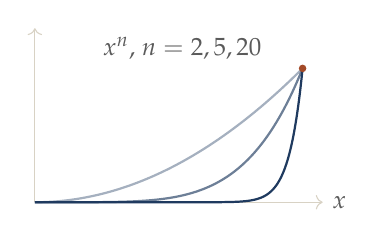
\begin{tikzpicture}[scale=0.85]
\draw[->,linie] (0,0)--(4.3,0) node[right,grau,font=\small] {$x$};
\draw[->,linie] (0,0)--(0,2.6);
\foreach \n/\c in {2/tief!40,5/tief!65,20/tief} {\draw[\c,thick,domain=0:4,samples=200,smooth] plot (\x,{2*(\x/4)^\n});}
\node[grau,font=\small] at (2.2,2.3) {$x^{n}$, $n = 2, 5, 20$};
\fill[akzent] (4,2) circle (1.6pt);
\end{tikzpicture}
\qquad
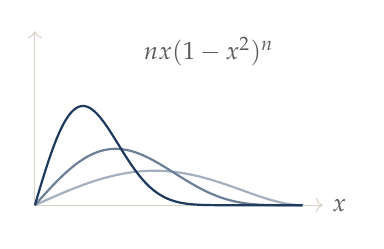
\begin{tikzpicture}[scale=0.85]
\draw[->,linie] (0,0)--(4.3,0) node[right,grau,font=\small] {$x$};
\draw[->,linie] (0,0)--(0,2.6);
\foreach \n/\c in {2/tief!40,5/tief!65,15/tief} {\draw[\c,thick,domain=0:4,samples=200,smooth] plot (\x,{0.9*\n*(\x/4)*(1-(\x/4)^2)^\n});}
\node[grau,font=\small] at (2.6,2.3) {$nx(1 - x^{2})^{n}$};
\end{tikzpicture}
\end{center}
\begin{fehler}\kastentext
\enquote{Für jedes $x$ gilt $f_n(x)\to f(x)$} ist eine Aussage über jeden Punkt einzeln; die Geschwindigkeit darf von $x$ abhängen. Gleichmäßig heißt: \emph{eine} Geschwindigkeit für alle $x$. Nur dann darf man $\lim$ mit $\int$, mit Stetigkeit, mit Reihen vertauschen --- und für Ableitungen auch dann nicht.
\end{fehler}
\begin{mitnehmen}\kastentext
Test auf gleichmäßige Konvergenz: $\sup_x|f_n(x) - f(x)|\to0$? Für Potenzreihen gilt sie auf jedem kompakten Teil des Konvergenzkreises, und deshalb darf man sie dort gliedweise integrieren und ableiten (Aufgabe 3.46). Die Buckelfolge (b) ist das Standardgegenbeispiel, das man kennen muss.
\end{mitnehmen}
\end{loesungkarte}

%%%%%%%%%% 3.46
\stupserzwei{gruen}{$\sum kx^{k-1} = \frac1{(1 - x)^{2}}$; mit $x$ multiplizieren.}{22pt}
\begin{loesungkarte}{gruen}{3.46}{$\sum kx^{k}$}
\derweg{Geometrische Reihe gliedweise ableiten, dann mit $x$ multiplizieren.}
\schritt{Ableiten}
$\sum_{k\ge0}x^{k} = \frac1{1 - x}$ für $|x| < 1$. Potenzreihen darf man im Inneren des Konvergenzkreises gliedweise ableiten (gleichmäßige Konvergenz auf kompakten Teilmengen): $\sum_{k\ge1}kx^{k-1} = \frac1{(1 - x)^{2}}$.
\schritt{Multiplizieren}
$\sum_{k\ge1}kx^{k} = \frac x{(1 - x)^{2}}$, $|x| < 1$.
\schritt{Anwendung}
$x = \frac12$: $\sum\frac k{2^{k}} = \frac{1/2}{1/4} = 2$.
\probe{$\frac12 + \frac24 + \frac38 + \frac4{16} + \frac5{32} + \frac6{64} = 0{,}5 + 0{,}5 + 0{,}375 + 0{,}25 + 0{,}156 + 0{,}094 = 1{,}875$, Rest $\approx0{,}125$. \checkmark\ (Deutung: erwartete Zahl der Würfe bis zum ersten Kopf, Gebiet 4.)}
\begin{mitnehmen}\kastentext
Aus $\frac1{1 - x}$ entstehen durch Ableiten $\sum kx^{k-1}$, $\sum k(k - 1)x^{k-2}$, \dots, durch Integrieren $-\ln(1 - x) = \sum\frac{x^{k}}k$ und $\arctan x$ (aus $\frac1{1 + x^{2}}$). Eine Reihe, eine Erlaubnis zum Vertauschen, eine ganze Familie geschlossener Formeln.
\end{mitnehmen}
\end{loesungkarte}

%%%%%%%%%% 3.47
\stupserzwei{tief}{$\nabla f(1, 0) = (0, 2)$. Richtungsableitung $(0, 2)\cdot\frac{(1, 1)}{\sqrt2} = \sqrt2$. Tangentialebene $z = 1 + 2y$.}{22pt}
\begin{loesungkarte}{tief}{3.47}{Gradient, Richtung, Tangentialebene}
\derweg{Partielle Ableitungen, einsetzen; Richtungsableitung als Skalarprodukt mit dem Einheitsvektor; lineare Näherung.}
\schritt{(a)}
$f_x = 2xy + ye^{xy}$, $f_y = x^{2} + xe^{xy}$. Bei $(1, 0)$: $f_x = 0 + 0 = 0$, $f_y = 1 + 1 = 2$. $\nabla f(1, 0) = (0, 2)$. Außerdem $f(1, 0) = 0 + 1 = 1$.
\schritt{(b)}
Einheitsvektor $e = \frac1{\sqrt2}(1, 1)$. $\partial_ef = \nabla f\cdot e = \frac{0 + 2}{\sqrt2} = \sqrt2\approx1{,}41$. Stärkster Anstieg in Richtung des Gradienten, also $(0, 1)$, mit Steigung $\|\nabla f\| = 2$. In Richtung $(1, 0)$ ändert sich $f$ in erster Ordnung nicht.
\schritt{(c)}
Tangentialebene: $z = f(1, 0) + f_x\cdot(x - 1) + f_y\cdot(y - 0) = 1 + 2y$. Näherung $f(1{,}1;\ 0{,}05)\approx1 + 2\cdot0{,}05 = 1{,}1$.
\probe{Exakt: $f(1{,}1;\ 0{,}05) = 1{,}21\cdot0{,}05 + e^{0{,}055} = 0{,}0605 + 1{,}0565 = 1{,}117$. Näherung $1{,}1$, Fehler $0{,}017$, quadratisch klein in der Schrittweite. \checkmark\ Richtungsableitung numerisch: $\frac{f(1 + 0{,}001/\sqrt2,\ 0{,}001/\sqrt2) - 1}{0{,}001} = 1{,}415$. \checkmark}
\begin{mitnehmen}\kastentext
Der Gradient zeigt in die Richtung des steilsten Anstiegs, seine Länge ist diese Steigung, und er steht senkrecht auf den Niveaulinien. Richtungsableitung $=$ Gradient mal Einheitsvektor; Tangentialebene $=$ Taylorpolynom ersten Grades. Alles aus Kapitel 6, nur mit Vektoren.
\end{mitnehmen}
\end{loesungkarte}

%%%%%%%%%% 3.48
\stupserzwei{gruen}{$(0, 0)$: $\det H = -9 < 0$, Sattel. $(1, 1)$: $\det H = 27 > 0$, $f_{xx} = 6 > 0$, Minimum mit $f = -1$.}{22pt}
\begin{loesungkarte}{gruen}{3.48}{Kritische Punkte klassifizieren}
\derweg{Gradient null setzen und lösen; Hesse-Matrix an jedem Punkt; Determinante und Vorzeichen von $f_{xx}$.}
\schritt{Kritische Punkte}
$f_x = 3x^{2} - 3y = 0\Rightarrow y = x^{2}$; $f_y = -3x + 3y^{2} = 0\Rightarrow x = y^{2} = x^{4}$. Also $x(x^{3} - 1) = 0$: $x = 0$ oder $x = 1$. Punkte $(0, 0)$ und $(1, 1)$.
\schritt{Hesse-Matrix}
$H = \begin{pmatrix}6x & -3\\ -3 & 6y\end{pmatrix}$.
\schritt{Klassifikation}
$(0, 0)$: $H = \begin{pmatrix}0 & -3\\ -3 & 0\end{pmatrix}$, $\det = -9 < 0$: indefinit, \emph{Sattelpunkt}, $f = 0$. (Entlang $y = x$: $f = 2x^{3} - 3x^{2} < 0$ für kleine $x > 0$; entlang $y = -x$: $f = 3x^{2} > 0$.) \\
$(1, 1)$: $H = \begin{pmatrix}6 & -3\\ -3 & 6\end{pmatrix}$, $\det = 27 > 0$, $f_{xx} = 6 > 0$: positiv definit, \emph{lokales Minimum}, $f(1, 1) = 1 - 3 + 1 = -1$.
\probe{$f(1{,}1;\ 1) = 1{,}331 - 3{,}3 + 1 = -0{,}969 > -1$; $f(1;\ 0{,}9) = 1 - 2{,}7 + 0{,}729 = -0{,}971 > -1$. \checkmark\ Kein globales Minimum: $f(x, 0) = x^{3}\to-\infty$.}
\begin{mitnehmen}\kastentext
Zwei Variablen: $\det H > 0$ und $f_{xx} > 0$ Minimum, $\det H > 0$ und $f_{xx} < 0$ Maximum, $\det H < 0$ Sattel, $\det H = 0$ keine Entscheidung. Die Eigenwerte der Hesse-Matrix (Gebiet 2) sagen dasselbe: beide positiv, beide negativ, gemischt.
\end{mitnehmen}
\end{loesungkarte}

%%%%%%%%%% 3.49
\stupserzwei{gruen}{Aus $y = \lambda$ und $x = \lambda$ folgt $x = y$; mit $x + y = 10$: $x = y = 5$.}{22pt}
\begin{loesungkarte}{gruen}{3.49}{Lagrange am Rechteck}
\derweg{$\nabla f = \lambda\nabla g$ plus Nebenbedingung; drei Gleichungen, drei Unbekannte.}
\schritt{Ansatz}
Maximiere $f(x, y) = xy$ unter $g(x, y) = x + y - 10 = 0$. $\nabla f = (y, x)$, $\nabla g = (1, 1)$.
\schritt{Lagrange}
$y = \lambda$, $x = \lambda$, $x + y = 10$. Also $x = y = 5$, $\lambda = 5$. Fläche $25$: das Quadrat.
\schritt{Vergleich}
Einsetzen: $y = 10 - x$, $A(x) = x(10 - x) = 10x - x^{2}$, $A' = 10 - 2x = 0$, $x = 5$. Dasselbe, hier sogar schneller. Lagrange zahlt sich aus, wenn man die Nebenbedingung nicht auflösen kann oder will --- und bei mehr als zwei Variablen.
\probe{$x = 4$, $y = 6$: Fläche $24 < 25$. $x = 5{,}5$, $y = 4{,}5$: $24{,}75 < 25$. \checkmark\ Deutung von $\lambda = 5$: Erhöht man den Umfang um $2$ (also $x + y$ um $1$), wächst die Maximalfläche um etwa $\lambda = 5$ ($6^{2} - 5^{2} = 11$ für Umfang $24$; für kleine Änderungen stimmt $\lambda$). \checkmark}
\begin{mitnehmen}\kastentext
Im Optimum berühren sich die Niveaulinie von $f$ und die Nebenbedingungskurve --- ihre Normalen (Gradienten) sind parallel. Das ist die ganze Geometrie hinter $\nabla f = \lambda\nabla g$. Der Multiplikator $\lambda$ misst, wie stark das Optimum auf eine Lockerung der Nebenbedingung reagiert.
\end{mitnehmen}
\end{loesungkarte}

%%%%%%%%%% 3.50
\stupserzwei{gruen}{$\int_0^1r^{2}\,dr = \frac13$, $\int_0^{\pi}\sin\vartheta\,d\vartheta = 2$, $\int_0^{2\pi}d\varphi = 2\pi$.}{22pt}
\begin{loesungkarte}{gruen}{3.50}{Das Volumen der Kugel}
\derweg{Kugelkoordinaten mit Funktionaldeterminante $r^{2}\sin\vartheta$; Fubini zerlegt in drei eindimensionale Integrale.}
\schritt{Koordinaten}
$x = r\sin\vartheta\cos\varphi$, $y = r\sin\vartheta\sin\varphi$, $z = r\cos\vartheta$; $r\in[0, 1]$, $\vartheta\in[0, \pi]$, $\varphi\in[0, 2\pi]$. Funktionaldeterminante $|\det J| = r^{2}\sin\vartheta$.
\schritt{Integral}
\begin{align*} V &= \int_0^{2\pi}\!\!\int_0^{\pi}\!\!\int_0^1r^{2}\sin\vartheta\,dr\,d\vartheta\,d\varphi\\ &= \Bigl(\int_0^1r^{2}\,dr\Bigr)\Bigl(\int_0^{\pi}\sin\vartheta\,d\vartheta\Bigr)\Bigl(\int_0^{2\pi}d\varphi\Bigr) = \frac13\cdot2\cdot2\pi = \frac{4\pi}3 . \end{align*}
\schritt{Woher die Faktoren kommen}
$\frac13$: das Volumen wächst wie $r^{3}$ (Kugel vom Radius $R$: $\frac43\pi R^{3}$). $2$: die Breite der Kugel in $z$-Richtung, als Mittelwert von $\sin\vartheta$ genommen. $2\pi$: der volle Umlauf.
\probe{Scheibenmethode: $V = \int_{-1}^{1}\pi(1 - z^{2})\,dz = \pi\bigl[z - \frac{z^{3}}3\bigr]_{-1}^{1} = \pi\bigl(2 - \frac23\bigr) = \frac{4\pi}3$. \checkmark\ Zahlenwert $4{,}189$; der Würfel $[-1, 1]^{3}$ hat Volumen $8$, die Kugel füllt $52\,\%$. \checkmark}
\begin{mitnehmen}\kastentext
Transformationssatz: $\int f\,dV = \int f(\Phi)\,|\det J_\Phi|\,du$. Die Funktionaldeterminante ist das Volumen des kleinen verzerrten Quaders --- bei Kugelkoordinaten $r^{2}\sin\vartheta$, bei Zylinderkoordinaten $r$, bei Polarkoordinaten $r$. Dann Fubini, und wenn der Integrand ein Produkt ist, zerfällt alles in Faktoren.
\end{mitnehmen}
\end{loesungkarte}

\cleardoublepage
\setgebiet{5}{Wahrscheinlichkeit}{mittel}
\chapter{Lösungen: Wahrscheinlichkeit}

%%%%%%%%%% 4.1
\stupserzwei{tief}{(b) Günstig für \enquote{verschieden, Maximum $6$}: $(6, k)$ und $(k, 6)$ mit $k = 1, \dots, 5$ --- zehn Paare.}{22pt}
\begin{loesungkarte}{tief}{4.1}{Würfel, Münzen, Karten: zählen}
\derweg{Grundraum mit gleich wahrscheinlichen Ergebnissen festlegen, günstige zählen, teilen.}
\schritt{(a)}
$2^{3} = 8$ gleich wahrscheinliche Folgen. Genau zweimal Kopf: KKZ, KZK, ZKK --- drei. $P = \frac38$.
\schritt{(b)}
$36$ geordnete Paare. Pasch: $(1, 1), \dots, (6, 6)$, sechs: $P = \frac6{36} = \frac16$. Verschieden mit Maximum $6$: $(6, k)$ und $(k, 6)$ für $k = 1, \dots, 5$, zehn: $P = \frac{10}{36} = \frac5{18}$.
\schritt{(c)}
$\binom{32}2 = 496$ Paare, davon $\binom42 = 6$ aus Assen: $P = \frac6{496} = \frac3{248}\approx0{,}0121$. Oder schrittweise: $\frac4{32}\cdot\frac3{31} = \frac{12}{992}$, dasselbe.
\schritt{(d)}
Als \emph{geordnete} Paare: Summe $2$ nur $(1, 1)$; Summe $3$ aber $(1, 2)$ und $(2, 1)$. Die Kombination $\{1, 2\}$ kann auf zwei Arten entstehen, $\{1, 1\}$ nur auf eine. Wer ungeordnete Paare zählt ($21$ Stück), hat keinen Laplace-Raum: Die $21$ Kombinationen sind nicht gleich wahrscheinlich.
\probe{(b) Die sechs Pasch-Paare plus die $30$ Nicht-Pasch-Paare sind $36$. Unter den $30$ hat jedes Maximum $m$ genau $2(m - 1)$ Paare: $0 + 2 + 4 + 6 + 8 + 10 = 30$. \checkmark}
\begin{mitnehmen}\kastentext
Laplace funktioniert nur, wenn alle Elementarereignisse gleich wahrscheinlich sind --- bei Würfeln und Münzen heißt das: geordnet zählen, auch wenn die Würfel nicht unterscheidbar aussehen. Der Fehler von d'Alembert (der $P(\text{einmal Kopf bei zwei Würfen}) = \frac13$ rechnete) ist genau dieser.
\end{mitnehmen}
\end{loesungkarte}

%%%%%%%%%% 4.2
\stupserzwei{gruen}{$\binom nk\cdot\frac{(n - k)!}{n!} = \frac1{k!}$ --- der Binomialkoeffizient kürzt fast alles weg.}{22pt}
\begin{loesungkarte}{gruen}{4.2}{Die vertauschten Briefe}
\derweg{Einschluss--Ausschluss über die Ereignisse \enquote{Brief $i$ richtig}; die Summe wird die Exponentialreihe von $-1$.}
\schritt{Ereignisse}
$A_i$ = \enquote{Brief $i$ liegt richtig}. Gesucht $P(\bigcap A_i^{c}) = 1 - P(\bigcup A_i)$.
\schritt{Schnitte}
$n!$ Verteilungen, alle gleich wahrscheinlich. Liegen $k$ bestimmte Briefe richtig, sind die übrigen $n - k$ beliebig: $(n - k)!$ Möglichkeiten. Also $P(A_{i_1}\cap\dots\cap A_{i_k}) = \frac{(n - k)!}{n!}$, und es gibt $\binom nk$ solche Schnitte.
\schritt{Einschluss--Ausschluss}
\[ P\Bigl(\bigcup A_i\Bigr) = \sum_{k=1}^{n}(-1)^{k+1}\binom nk\frac{(n - k)!}{n!} = \sum_{k=1}^{n}\frac{(-1)^{k+1}}{k!}, \]
also $P(\text{kein Brief richtig}) = 1 - \sum_{k=1}^{n}\frac{(-1)^{k+1}}{k!} = \sum_{k=0}^{n}\frac{(-1)^{k}}{k!}$.
\schritt{Grenzwert}
Das sind die Partialsummen der Reihe $e^{-1} = \sum\frac{(-1)^{k}}{k!}$. Für $n\to\infty$: $P\to\frac1e\approx0{,}3679$. Schon für $n = 6$ stimmt der Wert auf vier Stellen.
\probe{$n = 2$: $\frac12$ (von zwei Vertauschungen eine komplett falsch). \checkmark\ $n = 3$: $1 - 1 + \frac12 - \frac16 = \frac13$; von sechs Permutationen sind zwei fixpunktfrei ($231$, $312$). \checkmark\ $n = 4$: $\frac38$; $9$ von $24$. \checkmark}
\begin{mitnehmen}\kastentext
Dass die Antwort nicht von $n$ abhängt, ist das Verblüffende: Ob $10$ Briefe oder $10\,000$, in $37\,\%$ der Fälle liegt kein einziger richtig. Die fixpunktfreien Permutationen heißen Derangements, ihre Anzahl $D_n = n!\sum_{k\le n}\frac{(-1)^{k}}{k!}$ ist die zu $\frac{n!}e$ nächste ganze Zahl.
\end{mitnehmen}
\end{loesungkarte}

%%%%%%%%%% 4.3
\stupserzwei{tief}{(d) Zweiter Fall: \enquote{mindestens eine Vier} sind $11$ Paare; \enquote{Summe $7$} darunter: $(3, 4)$ und $(4, 3)$.}{22pt}
\begin{loesungkarte}{tief}{4.3}{Zwei Würfel, eine Summe}
\derweg{Die $6\times6$-Tabelle; Summen liegen auf Diagonalen.}
\schritt{(a)}
Anzahl Paare mit Summe $k$: $1, 2, 3, 4, 5, 6, 5, 4, 3, 2, 1$ für $k = 2, \dots, 12$. Also $P(S = k) = \frac{6 - |k - 7|}{36}$.
\begin{center}
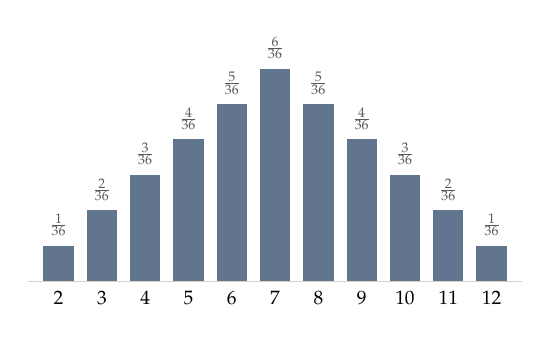
\begin{tikzpicture}[x=0.55cm,y=0.45cm]
\foreach \k/\h in {2/1,3/2,4/3,5/4,6/5,7/6,8/5,9/4,10/3,11/2,12/1} {\fill[tief!70] (\k-0.35,0) rectangle (\k+0.35,\h); \node[below,font=\scriptsize] at (\k,0) {\k}; \node[above,font=\tiny,grau] at (\k,\h) {$\frac{\h}{36}$};}
\draw[linie] (1.3,0)--(12.7,0);
\end{tikzpicture}
\end{center}
\schritt{(b)}
Am wahrscheinlichsten $S = 7$ mit $\frac6{36} = \frac16$. $P(S\ge10) = \frac{3 + 2 + 1}{36} = \frac16$.
\schritt{(c)}
Gewinn ($7$ oder $11$): $\frac{6 + 2}{36} = \frac29\approx22\,\%$. Verlust ($2$, $3$, $12$): $\frac{1 + 2 + 1}{36} = \frac19\approx11\,\%$. Die übrigen $\frac23$ führen zum Weiterspiel.
\schritt{(d)}
Erster Würfel $4$: Der zweite muss $3$ zeigen, $P = \frac16$. Mindestens ein Würfel $4$: $11$ Paare (sechs mit $4$ vorn, sechs mit $4$ hinten, $(4, 4)$ doppelt gezählt). Summe $7$ darunter: $(4, 3)$, $(3, 4)$. $P = \frac2{11}\approx0{,}18$ --- mehr als $\frac16$, weil die Bedingung die Pasch-Lücke $(4, 4)$ nicht ausgleicht.
\probe{Summe aller $P(S = k)$: $\frac{1 + 2 + \dots + 6 + 5 + \dots + 1}{36} = \frac{36}{36}$. \checkmark\ $E[S] = 7$ aus Symmetrie. \checkmark}
\begin{mitnehmen}\kastentext
Die Verteilung der Summe zweier Gleichverteilungen ist dreieckig --- die erste Faltung. Mit drei Würfeln wird sie schon glockenförmig: der zentrale Grenzwertsatz in Kinderschuhen (Aufgabe 4.32).
\end{mitnehmen}
\end{loesungkarte}

%%%%%%%%%% 4.4
\stupserzwei{gruen}{$\binom{32}{10} = 64\,512\,240$, $\binom{28}7 = 1\,184\,040$, $\binom{28}6 = 376\,740$, $\binom{24}2 = 276$.}{22pt}
\begin{loesungkarte}{gruen}{4.4}{Zehn Karten aus dem Skatblatt}
\derweg{Hypergeometrisch: Buben aus den Buben, Rest aus dem Rest, durch alle Blätter.}
\schritt{Grundraum}
$|\Omega| = \binom{32}{10} = 64\,512\,240$ Blätter, ungeordnet, ohne Zurücklegen, alle gleich wahrscheinlich.
\schritt{(a)}
$3$ der $4$ Buben und $7$ der $28$ Nicht-Buben: $\binom43\binom{28}7 = 4\cdot1\,184\,040 = 4\,736\,160$. $P = \frac{4\,736\,160}{64\,512\,240} = 0{,}0734$.
\schritt{(b)}
Dazu genau $4$ Buben: $\binom44\binom{28}6 = 376\,740$. $P(\ge3) = \frac{4\,736\,160 + 376\,740}{64\,512\,240} = \frac{5\,112\,900}{64\,512\,240} = 0{,}0793$.
\schritt{(c)}
Alle $8$ Karo plus $2$ aus den übrigen $24$: $\binom88\binom{24}2 = 276$. $P = \frac{276}{64\,512\,240} = 4{,}3\cdot10^{-6}$ --- etwa einmal in $234\,000$ Blättern.
\probe{Erwartete Bubenzahl $10\cdot\frac4{32} = 1{,}25$; drei oder mehr sollte selten sein, $8\,\%$ passt. \checkmark\ (c) schrittweise: $\frac{10}{32}\cdot\frac9{31}\cdots\frac3{25}$ für die ersten $8$ Karten Karo, mal $\binom{10}8$ für die Position --- dasselbe Ergebnis. \checkmark}
\begin{mitnehmen}\kastentext
Hypergeometrische Verteilung: $P(X = k) = \binom Mk\binom{N - M}{n - k}/\binom Nn$ --- $M$ Erfolge in der Urne, $n$ gezogen, $k$ Erfolge in der Hand. \enquote{Mindestens} summiert man direkt, wenn wenige Terme, sonst über das Gegenteil.
\end{mitnehmen}
\end{loesungkarte}

%%%%%%%%%% 4.5
\stupserzwei{gruen}{$n = 22$: $0{,}476$; $n = 23$: $0{,}507$. Die Schwelle liegt genau dazwischen.}{22pt}
\begin{loesungkarte}{gruen}{4.5}{Gleiche Geburtstage}
\derweg{Das Gegenteil --- alle Geburtstage verschieden --- als Produkt berechnen und von eins abziehen.}
\schritt{(a), (b)}
Die zweite Person muss einen der $364$ übrigen Tage treffen: $\frac{364}{365} = 0{,}9973$. Die dritte einen der $363$ übrigen: $\frac{364}{365}\cdot\frac{363}{365} = 0{,}9918$.
\schritt{(c)}
\[ P(\text{alle verschieden}) = \frac{365}{365}\cdot\frac{364}{365}\cdots\frac{365 - n + 1}{365} = \prod_{k=0}^{n-1}\Bigl(1 - \frac k{365}\Bigr). \]
$n = 22$: $0{,}5243$, also $47{,}6\,\%$ für einen gemeinsamen Geburtstag. $n = 23$: $0{,}4927$, also $50{,}7\,\%$. Das kleinste $n$ ist $23$.
\begin{center}
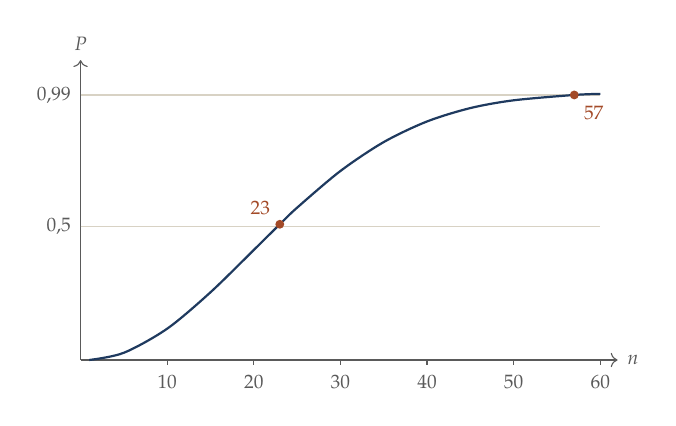
\begin{tikzpicture}[x=0.11cm,y=3.4cm,font=\small]
\draw[grau,->] (0,0)--(62,0) node[right,font=\scriptsize]{$n$};
\draw[grau,->] (0,0)--(0,1.12) node[above,font=\scriptsize]{$P$};
\foreach \y/\l in {0.5/{$0{,}5$},0.99/{$0{,}99$}} {\draw[linie] (0,\y)--(60,\y); \node[left,font=\scriptsize,grau] at (0,\y) {\l};}
\foreach \x in {10,20,30,40,50,60} {\draw[grau] (\x,0)--(\x,-0.02); \node[below,font=\scriptsize,grau] at (\x,-0.02) {\x};}
\draw[tief,thick] plot[smooth] coordinates {(1,0) (5,0.027) (10,0.117) (15,0.253) (20,0.411) (23,0.507) (25,0.569) (30,0.706) (35,0.814) (40,0.891) (45,0.941) (50,0.970) (57,0.990) (60,0.994)};
\fill[akzent] (23,0.507) circle (1.6pt); \node[akzent,font=\scriptsize,above left] at (23,0.507) {$23$};
\fill[akzent] (57,0.990) circle (1.6pt); \node[akzent,font=\scriptsize,below right] at (57,0.985) {$57$};
\end{tikzpicture}
\end{center}
\schritt{(d)}
Bei $n = 57$: $P(\text{alle verschieden}) = 0{,}0099$, also $99{,}0\,\%$. Bei $n = 70$: $99{,}9\,\%$.
\schritt{(e)}
Unter $23$ Personen gibt es $\binom{23}2 = 253$ Paare. Jedes hat die Chance $\frac1{365}$; $253$ Versuche ergeben im Mittel $0{,}69$ Treffer. Die Intuition denkt an \emph{eine} Person, die mit $22$ anderen verglichen wird ($\frac{22}{365} = 6\,\%$) --- gefragt ist aber nach irgendeinem Paar.
\probe{Paarnäherung: $1 - (1 - \frac1{365})^{253} = 0{,}5005$, nahe am exakten $0{,}5073$; der Unterschied kommt daher, dass die Paare nicht unabhängig sind. \checkmark\ Näherung $P(\text{alle verschieden})\approx e^{-n(n - 1)/730}$: für $n = 23$ gibt das $e^{-0{,}693} = 0{,}500$. \checkmark}
\begin{mitnehmen}\kastentext
\enquote{Mindestens einmal} rechnet man über das Gegenteil. Die Kurve steigt wie $n^{2}$, weil jede neue Person sich mit allen bisherigen vergleicht --- und das ist auch der Grund, warum Hash-Kollisionen so viel früher auftreten, als man denkt (Geburtstagsangriff, Band 1).
\end{mitnehmen}
\end{loesungkarte}

%%%%%%%%%% 4.6
\stupserzwei{gruen}{$\binom{m + n}m$: Von den $m + n$ Positionen wählt man die $m$ für R aus.}{22pt}
\begin{loesungkarte}{gruen}{4.6}{Wege im Gitter}
\derweg{Weg $=$ Wort aus $m$ R und $n$ O; Wörter zählen durch Auswahl der R-Positionen.}
Jeder Weg besteht aus genau $m$ Schritten nach rechts und $n$ nach oben, in irgendeiner Reihenfolge --- ein Wort der Länge $m + n$ mit $m$ Buchstaben R. Die Positionen der R wählen: $\binom{m + n}m = \binom{m + n}n$ Wege.

Für $(2, 2)$: $\binom42 = 6$: RROO, RORO, ROOR, ORRO, OROR, OORR. \checkmark
\probe{Rekursion: Nach $(m, n)$ kommt man von $(m - 1, n)$ oder $(m, n - 1)$: $W(m, n) = W(m - 1, n) + W(m, n - 1)$ --- die Pascal-Regel $\binom{m + n}m = \binom{m + n - 1}{m - 1} + \binom{m + n - 1}m$. \checkmark}
\begin{mitnehmen}\kastentext
Gitterwege sind die Geometrie des Binomialkoeffizienten; das Pascalsche Dreieck ist eine um $45^{\circ}$ gedrehte Wegezählung. Mit einer Zusatzbedingung (nie über die Diagonale) werden daraus die Catalan-Zahlen, mit Schritten $\pm1$ die Irrfahrt aus Kapitel 13.
\end{mitnehmen}
\end{loesungkarte}

%%%%%%%%%% 4.7
\stupserzwei{akzent}{(d) $1 - \bigl(\frac{35}{36}\bigr)^{n} > \frac12\iff n > \frac{\ln2}{-\ln(35/36)} = 24{,}6$. Mit $25$ Würfen hätte de Méré gewonnen.}{22pt}
\begin{loesungkarte}{akzent}{4.7}{\enquote{Mindestens eine Sechs}}
\derweg{Gegenwahrscheinlichkeit; dann klären, was die Summe der Einzelwahrscheinlichkeiten wirklich ist.}
\schritt{(a)}
$P(\text{keine Sechs in 4 Würfen}) = \bigl(\frac56\bigr)^{4} = 0{,}4823$, also $P(\text{mindestens eine}) = 0{,}5177$. Günstig --- de Méré gewann zu Recht.
\schritt{(b)}
$P(\text{keine Doppelsechs in 24 Würfen}) = \bigl(\frac{35}{36}\bigr)^{24} = 0{,}5086$, also $P(\text{mindestens eine}) = 0{,}4914$. Ungünstig --- er verlor zu Recht, wenn auch knapp.
\schritt{(c)}
$4\cdot\frac16 = \frac23$ ist der \emph{Erwartungswert} der Anzahl Sechsen in vier Würfen (Aufgabe 4.20), nicht die Wahrscheinlichkeit für mindestens eine. $P(A\cup B) = P(A) + P(B)$ gilt nur für \emph{unvereinbare} $A, B$; die Ereignisse \enquote{Sechs im $i$-ten Wurf} können gleichzeitig eintreten. Allgemein $P(A\cup B) = P(A) + P(B) - P(A\cap B)$, und die Additivität überschätzt --- mit $36$ Doppelwürfen gäbe sie $P = 1$.
\schritt{(d)}
$\bigl(\frac{35}{36}\bigr)^{n} < \frac12\iff n > \frac{\ln2}{\ln(36/35)} = \frac{0{,}6931}{0{,}02817} = 24{,}6$. Ab $25$ Würfen ist die Wette günstig: $1 - (35/36)^{25} = 0{,}5055$.
\probe{(a) über Einschluss--Ausschluss: $4\cdot\frac16 - 6\cdot\frac1{36} + 4\cdot\frac1{216} - \frac1{1296} = 0{,}6667 - 0{,}1667 + 0{,}0185 - 0{,}0008 = 0{,}5177$. \checkmark}
\begin{fehler}\kastentext
Wahrscheinlichkeiten addieren sich nur bei unvereinbaren Ereignissen. \enquote{Mindestens einmal in $n$ Versuchen} ist $1 - (1 - p)^{n}$, und das ist für kleine $np$ ungefähr $np$ --- deshalb funktioniert die Faustregel bei einem Wurf und versagt bei vielen.
\end{fehler}
\begin{mitnehmen}\kastentext
Die Korrespondenz zwischen Pascal und Fermat über de Mérés Fragen (1654) gilt als Geburtsstunde der Wahrscheinlichkeitsrechnung. Die Lektion ist noch dieselbe: Wer \enquote{mindestens} hört, rechnet das Gegenteil.
\end{mitnehmen}
\end{loesungkarte}

%%%%%%%%%% 4.8
\stupserzwei{tief}{(c) $P(R_1\mid R_2) = \frac{P(R_1\cap R_2)}{P(R_2)} = \frac{3/5\cdot2/4}{3/5} = \frac12$ --- dasselbe wie $P(R_2\mid R_1)$.}{22pt}
\begin{loesungkarte}{tief}{4.8}{Bedingt --- in welche Richtung?}
\derweg{Baum zeichnen; Pfadwahrscheinlichkeiten multiplizieren; bedingen heißt: einen Teilbaum zum neuen Ganzen machen.}
\schritt{(a)}
Erste Kugel rot ($\frac35$) oder blau ($\frac25$). Nach einer roten bleiben $2$ rote und $2$ blaue: $P(R_2\mid R_1) = \frac24 = \frac12$.
\begin{center}
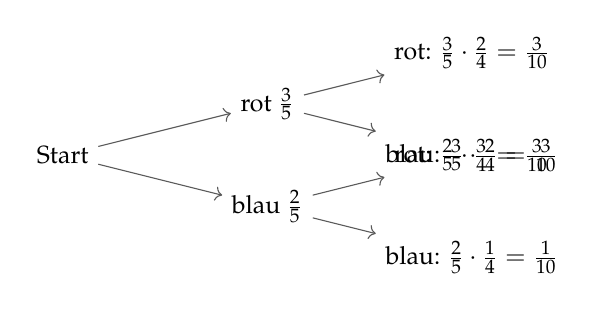
\begin{tikzpicture}[font=\small,grow=right,level distance=2.6cm,sibling distance=1.3cm,edge from parent/.style={draw,grau,->}]
\node {Start}
  child {node {blau $\frac25$} child {node {blau: $\frac25\cdot\frac14 = \frac1{10}$}} child {node {rot: $\frac25\cdot\frac34 = \frac3{10}$}}}
  child {node {rot $\frac35$} child {node {blau: $\frac35\cdot\frac24 = \frac3{10}$}} child {node {rot: $\frac35\cdot\frac24 = \frac3{10}$}}};
\end{tikzpicture}
\end{center}
\schritt{(b)}
$P(R_2) = P(R_1)P(R_2\mid R_1) + P(B_1)P(R_2\mid B_1) = \frac35\cdot\frac24 + \frac25\cdot\frac34 = \frac3{10} + \frac3{10} = \frac35$. Gleich $P(R_1)$: Ohne Information über den ersten Zug ist der zweite genauso verteilt wie der erste.
\schritt{(c)}
$P(R_1\mid R_2) = \frac{P(R_1\cap R_2)}{P(R_2)} = \frac{3/10}{3/5} = \frac12$. Die Information läuft rückwärts, aber Bayes stört das nicht.
\schritt{(d)}
(a) und (c) sind beide $\frac12$: Die Ziehung ist \emph{austauschbar} --- die Reihenfolge spielt für die gemeinsame Verteilung keine Rolle, also sind $P(R_2\mid R_1)$ und $P(R_1\mid R_2)$ gleich. Das ist eine Besonderheit dieses Beispiels, kein allgemeines Gesetz; bei Aufgabe 4.10 sind $P(T^{+}\mid K) = 0{,}9$ und $P(K\mid T^{+}) = 0{,}09$ grundverschieden. (b) ist $\frac35$ und etwas anderes: unbedingt.
\probe{Die vier Pfade summieren sich zu $\frac1{10} + \frac3{10} + \frac3{10} + \frac3{10} = 1$. \checkmark}
\begin{mitnehmen}\kastentext
$P(A\mid B)$: $B$ ist das neue Ganze, $A\cap B$ der Teil davon. Im Baum heißt das: die Pfade durch $B$ sammeln, die durch $A\cap B$ darunter zählen. Die Richtung der Bedingung ist im Alltag die häufigste Fehlerquelle --- vom Testergebnis bis zum $p$-Wert (Aufgabe 4.40).
\end{mitnehmen}
\end{loesungkarte}

%%%%%%%%%% 4.9
\stupserzwei{akzent}{(d) $E$ muss zwei Elemente haben, davon genau eines gerade: $3\cdot3 = 9$ solche Mengen. Für $P(E) = \frac12$ bräuchte man $P(A\cap E) = \frac14$, also $1{,}5$ Elemente --- unmöglich.}{22pt}
\begin{loesungkarte}{akzent}{4.9}{Unabhängig oder unvereinbar?}
\derweg{Beides nachrechnen: $P(A\cap B)$ mit $0$ vergleichen (unvereinbar) und mit $P(A)P(B)$ (unabhängig).}
\schritt{(a)}
$A = \{2, 4, 6\}$, $B = \{3, 6\}$, $A\cap B = \{6\}$. $P(A\cap B) = \frac16 = \frac12\cdot\frac13 = P(A)P(B)$: \emph{unabhängig}. Nicht unvereinbar ($6$ liegt in beiden).
\schritt{(b)}
$C\cap D = \emptyset$: \emph{unvereinbar}. $P(C\cap D) = 0\neq\frac13\cdot\frac13$: \emph{abhängig}. Weiß man, dass $C$ eingetreten ist, ist $D$ unmöglich --- stärker kann Abhängigkeit nicht sein.
\schritt{(c)}
Unvereinbar heißt $P(A\cap B) = 0$. Unabhängig hieße $P(A\cap B) = P(A)P(B) > 0$. Beides zugleich geht nicht. $\blacksquare$
\schritt{(d)}
$A\cap C = \{2\}$: $\frac16 = \frac12\cdot\frac13$, unabhängig. Allgemein ist $E$ mit $|E| = 2$ genau dann von $A$ unabhängig, wenn $|A\cap E| = 1$, also eine gerade und eine ungerade Zahl: $3\cdot3 = 9$ Mengen ($\{1, 2\}$, $\{1, 4\}$, \dots, $\{5, 6\}$). Für $P(E) = \frac12$ bräuchte man $|A\cap E| = \frac32$: Kein Ereignis mit Wahrscheinlichkeit $\frac12$ ist von $A$ unabhängig (außer über einem feineren Grundraum).
\begin{fehler}\kastentext
\enquote{Unabhängig} und \enquote{unvereinbar} werden verwechselt, weil beide nach \enquote{getrennt} klingen. Unvereinbar ist eine Aussage über Mengen (kein gemeinsames Element), unabhängig über Wahrscheinlichkeiten (Produktformel). Unvereinbare Ereignisse mit positiver Wahrscheinlichkeit sind immer abhängig.
\end{fehler}
\begin{mitnehmen}\kastentext
Unabhängigkeit ist keine Eigenschaft, die man einer Menge ansieht --- sie hängt vom Wahrscheinlichkeitsmaß ab. Bei einem gezinkten Würfel wären $A$ und $B$ aus (a) im Allgemeinen nicht mehr unabhängig.
\end{mitnehmen}
\end{loesungkarte}

%%%%%%%%%% 4.10
\stupserzwei{gruen}{$9$ Kranke und $89$ Gesunde testen positiv. Der Anteil der Kranken unter den Positiven ist $\frac9{98}$.}{22pt}
\begin{loesungkarte}{gruen}{4.10}{Ein positiver Test}
\derweg{Statt mit Prozenten zu rechnen, lässt man tausend Menschen durch den Test laufen und zählt.}
\schritt{(a), (b) --- der Häufigkeitsbaum}
Von $1000$ Personen sind $1\,\%$ krank: $10$. Die übrigen $990$ sind gesund. Von den $10$ Kranken testen $90\,\%$ positiv: $9$. Von den $990$ Gesunden testen $9\,\%$ falsch positiv: $89$.
\begin{center}
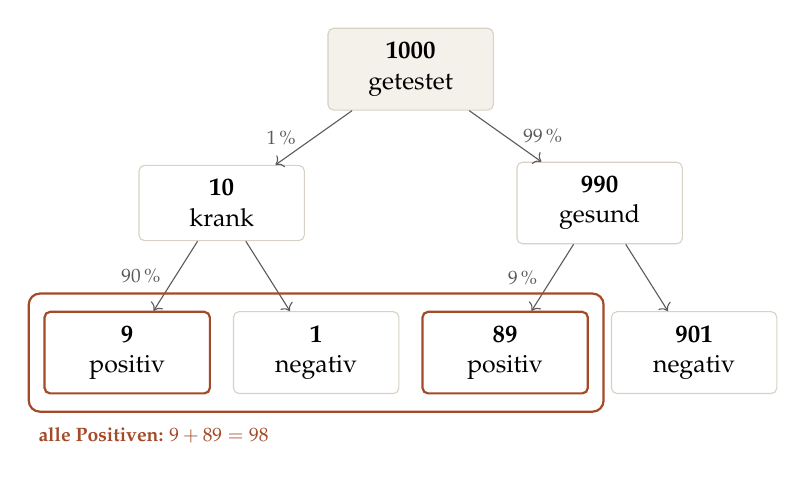
\begin{tikzpicture}[x=1cm,y=1cm,font=\small,
  kn/.style={draw=linie,fill=white,rounded corners=2pt,inner sep=5pt,align=center,minimum width=2.1cm},
  pf/.style={->,grau}]
\node[kn,fill=sand] (a) at (0,0) {\textbf{1000}\\getestet};
\node[kn] (k) at (-2.4,-1.7) {\textbf{10}\\krank};
\node[kn] (g) at (2.4,-1.7) {\textbf{990}\\gesund};
\node[kn,draw=akzent,thick] (kp) at (-3.6,-3.6) {\textbf{9}\\positiv};
\node[kn] (kn) at (-1.2,-3.6) {\textbf{1}\\negativ};
\node[kn,draw=akzent,thick] (gp) at (1.2,-3.6) {\textbf{89}\\positiv};
\node[kn] (gn) at (3.6,-3.6) {\textbf{901}\\negativ};
\draw[pf] (a)--(k) node[midway,left=3pt,font=\scriptsize]{$1\,\%$};
\draw[pf] (a)--(g) node[midway,right=3pt,font=\scriptsize]{$99\,\%$};
\draw[pf] (k)--(kp) node[midway,left=2pt,font=\scriptsize]{$90\,\%$};
\draw[pf] (k)--(kn);
\draw[pf] (g)--(gp) node[midway,left=2pt,font=\scriptsize]{$9\,\%$};
\draw[pf] (g)--(gn);
\draw[akzent,thick,rounded corners=4pt] (-4.85,-4.35) rectangle (2.45,-2.85);
\node[akzent,font=\scriptsize\bfseries,anchor=west] at (-4.85,-4.65) {alle Positiven: $9 + 89 = 98$};
\end{tikzpicture}
\end{center}
\schritt{(c) --- der positive Vorhersagewert}
Unter den $98$ Positiven sind $9$ krank: $\mathrm{PPV} = \frac9{98}\approx9{,}2\,\%$. Die Sensitivität $90\,\%$ beantwortet \enquote{Wenn krank, wie oft positiv?}; die Patientin fragt \enquote{Wenn positiv, wie oft krank?}. Umgekehrte Bedingung, zehnmal kleinere Antwort.
\schritt{(d) --- Prävalenz $10\,\%$}
$100$ krank, $90$ davon positiv; $900$ gesund, $81$ davon positiv. $\mathrm{PPV} = \frac{90}{171}\approx53\,\%$. Geändert hat sich nur die erste Verzweigung; Sensitivität und Falsch-Positiv-Rate sind dieselben.
\schritt{(e)}
Der Test bestimmt, wie viele Falschpositive je Gesundem anfallen; die Prävalenz bestimmt, wie viele Gesunde es gibt --- bei seltener Krankheit ertrinken die wenigen richtig Positiven in den vielen Gesunden.
\probe{$9 + 1 = 10$, $89 + 901 = 990$. \checkmark\ Bayes: $\frac{0{,}9\cdot0{,}01}{0{,}9\cdot0{,}01 + 0{,}09\cdot0{,}99} = \frac{0{,}009}{0{,}0981} = 0{,}0917$. \checkmark}
\begin{mitnehmen}\kastentext
Ein positiver Test bei seltener Krankheit ist meistens falsch --- nicht weil der Test schlecht wäre, sondern weil die Gesunden so viele sind. Rechnen Sie mit tausend Menschen, nie mit Prozenten; natürliche Häufigkeiten verstehen auch Patienten.
\end{mitnehmen}
\end{loesungkarte}

%%%%%%%%%% 4.11
\stupserzwei{gruen}{Wechseln gewinnt genau dann, wenn die erste Wahl falsch war --- und das ist in zwei von drei Fällen so.}{22pt}
\begin{loesungkarte}{gruen}{4.11}{Drei Türen}
\derweg{Annahmen aufschreiben, über die Autoposition fallunterscheiden, dann mit Bayes bestätigen.}
\schritt{(a) Annahmen}
(i) Das Auto steht gleichverteilt hinter einer der drei Türen. (ii) Der Kandidat wählt unabhängig davon (etwa Tür $1$). (iii) Der Moderator öffnet \emph{immer} eine nicht gewählte Tür mit Ziege; hat er zwei zur Auswahl, wählt er zufällig. Ohne (iii) ist die Aufgabe nicht gestellt.
\schritt{(b) Fallunterscheidung}
Kandidat wählt Tür $1$. Auto hinter $1$ ($\frac13$): bleiben gewinnt, wechseln verliert. Auto hinter $2$ ($\frac13$): Moderator muss $3$ öffnen; wechseln (auf $2$) gewinnt. Auto hinter $3$ ($\frac13$): Moderator muss $2$ öffnen; wechseln (auf $3$) gewinnt. Bleiben: $\frac13$. Wechseln: $\frac23$.
\schritt{(c) Bayes}
$M_3$ = \enquote{Moderator öffnet Tür $3$}. $P(M_3\mid A_1) = \frac12$, $P(M_3\mid A_2) = 1$, $P(M_3\mid A_3) = 0$. $P(M_3) = \frac13\cdot\frac12 + \frac13\cdot1 + 0 = \frac12$. $P(A_1\mid M_3) = \frac{\frac13\cdot\frac12}{\frac12} = \frac13$, $P(A_2\mid M_3) = \frac{\frac13\cdot1}{\frac12} = \frac23$. Wechseln.
\schritt{(d) Unwissender Moderator}
Er öffnet zufällig Tür $2$ oder $3$; wir beobachten: Tür $3$, Ziege. $P(M_3\cap\text{Ziege}\mid A_1) = \frac12$, $P(\dots\mid A_2) = \frac12$, $P(\dots\mid A_3) = 0$. Jetzt $P(A_1\mid\dots) = P(A_2\mid\dots) = \frac12$: Wechseln bringt nichts. Der Unterschied: Der wissende Moderator \emph{muss} bei $A_2$ die $3$ öffnen, der unwissende nur zufällig --- und diese Asymmetrie trägt die Information.
\probe{Simulation im Kopf mit $300$ Spielen: $100$-mal Auto hinter $1$, $100$-mal hinter $2$, $100$-mal hinter $3$. Wechsler gewinnen in den letzten $200$. \checkmark}
\begin{mitnehmen}\kastentext
Die Intuition \enquote{zwei Türen, $50 : 50$} ignoriert, dass die Tür des Moderators nicht zufällig war. Wo Information herkommt, entscheidet über ihren Wert --- dieselbe Lektion wie beim Simpson-Paradox (Aufgabe 4.12) und bei der Studienauswahl (Publication Bias).
\end{mitnehmen}
\end{loesungkarte}

%%%%%%%%%% 4.12
\stupserzwei{gruen}{$A$: $\frac{87}{350}\cdot0{,}931 + \frac{263}{350}\cdot0{,}730 = 0{,}231 + 0{,}549 = 0{,}780$. Das Gewicht liegt auf den großen Steinen --- den schwierigen Fällen.}{22pt}
\begin{loesungkarte}{gruen}{4.12}{Das Simpson-Paradox}
\derweg{Gesamtquote als gewichtetes Mittel der Teilquoten; die Gewichte sind das Paradox.}
\schritt{(a)}
$\frac{81}{87} = 0{,}931$, $\frac{234}{270} = 0{,}867$; $\frac{192}{263} = 0{,}730$, $\frac{55}{80} = 0{,}688$; $\frac{273}{350} = 0{,}780$, $\frac{289}{350} = 0{,}826$. Und $81 + 192 = 273$, $234 + 55 = 289$. \checkmark
\schritt{(b)}
$A$: $\frac{87}{350}\cdot\frac{81}{87} + \frac{263}{350}\cdot\frac{192}{263} = 0{,}249\cdot0{,}931 + 0{,}751\cdot0{,}730 = 0{,}780$. Gewichte: $25\,\%$ kleine, $75\,\%$ große Steine. \\
$B$: $\frac{270}{350}\cdot0{,}867 + \frac{80}{350}\cdot0{,}688 = 0{,}771\cdot0{,}867 + 0{,}229\cdot0{,}688 = 0{,}826$. Gewichte: $77\,\%$ kleine, $23\,\%$ große.
\schritt{(c)}
Die Steingröße ist die Störgröße (Confounder): Sie beeinflusst sowohl die Verfahrenswahl (große Steine bekamen meist $A$) als auch den Erfolg (große Steine heilen schlechter). $A$ wurde auf die schweren Fälle angesetzt und zieht deshalb in der Gesamtquote den Kürzeren --- obwohl es in jeder Gruppe besser ist.
\schritt{(d)}
$A$, auf Grundlage der nach Steingröße getrennten Tabelle. Die Teilquoten vergleichen Gleiches mit Gleichem; die Gesamtquote vergleicht \enquote{$A$ bei schweren Fällen} mit \enquote{$B$ bei leichten}. (Allgemein ist die Antwort nicht immer \enquote{getrennt}: Wäre die Gruppenvariable eine \emph{Folge} der Behandlung, müsste man zusammenfassen. Hier ist die Steingröße vorher da.)
\probe{Mit vertauschten Gewichten --- $A$ auf $77\,\%$ kleine --- hätte $A$ eine Gesamtquote von $0{,}771\cdot0{,}931 + 0{,}229\cdot0{,}730 = 0{,}885$: besser als $B$. Es sind die Gewichte. \checkmark}
\begin{mitnehmen}\kastentext
Simpsons Paradox entsteht immer, wenn eine dritte Variable mit beiden anderen zusammenhängt und die Gruppen ungleich besetzt sind. Randomisierung in Studien verhindert genau das: Sie macht die Gewichte in beiden Armen gleich. Beobachtungsdaten muss man stratifizieren --- und wissen, wonach.
\end{mitnehmen}
\end{loesungkarte}

%%%%%%%%%% 4.13
\stupserzwei{tief}{(c) $E[2X + 1] = 2\cdot3{,}5 + 1 = 8$, $\operatorname{Var}(2X + 1) = 4\operatorname{Var}X$ --- die Verschiebung ändert die Varianz nicht.}{22pt}
\begin{loesungkarte}{tief}{4.13}{Ein Würfel als Zufallsvariable}
\derweg{Verteilung als Tabelle, Verteilungsfunktion als Treppe, Momente durch Summen; lineare Transformationen über die Regeln.}
\schritt{(a)}
$P(X = k) = \frac16$ für $k = 1, \dots, 6$. $F(x) = 0$ für $x < 1$, $F(x) = \frac{\lfloor x\rfloor}6$ für $1\le x < 6$, $F(x) = 1$ für $x\ge6$: eine Treppe mit sechs Stufen der Höhe $\frac16$, rechtsseitig stetig.
\schritt{(b)}
$E[X] = \frac{1 + 2 + \dots + 6}6 = \frac{21}6 = 3{,}5$. $E[X^{2}] = \frac{1 + 4 + 9 + 16 + 25 + 36}6 = \frac{91}6$. $\operatorname{Var}X = \frac{91}6 - \frac{49}4 = \frac{182 - 147}{12} = \frac{35}{12}\approx2{,}917$, Standardabweichung $1{,}71$.
\schritt{(c)}
$E[Y] = 2E[X] + 1 = 8$. $\operatorname{Var}Y = 4\operatorname{Var}X = \frac{35}3\approx11{,}67$.
\schritt{(d)}
$Z = (X - 3)^{2}$ nimmt die Werte $4, 1, 0, 1, 4, 9$ an (für $X = 1, \dots, 6$). Verteilung: $P(Z = 0) = \frac16$, $P(Z = 1) = \frac26$, $P(Z = 4) = \frac26$, $P(Z = 9) = \frac16$. $E[Z] = \frac{0 + 2 + 8 + 9}6 = \frac{19}6\approx3{,}17$.
\probe{(d) anders: $E[(X - 3)^{2}] = \operatorname{Var}X + (E[X] - 3)^{2} = \frac{35}{12} + \frac14 = \frac{38}{12} = \frac{19}6$. \checkmark\ (Verschiebungssatz: Der mittlere quadratische Abstand von $c$ ist Varianz plus $(\mu - c)^{2}$, minimal bei $c = \mu$.)}
\begin{mitnehmen}\kastentext
$E[aX + b] = aE[X] + b$, $\operatorname{Var}(aX + b) = a^{2}\operatorname{Var}X$. Für nichtlineare $g$ gilt $E[g(X)] = \sum g(k)P(X = k)$ --- man braucht die Verteilung von $g(X)$ nicht aufzustellen. Und $E[g(X)]\neq g(E[X])$: $E[X^{2}] = 15{,}17\neq12{,}25$.
\end{mitnehmen}
\end{loesungkarte}

%%%%%%%%%% 4.14
\stupserzwei{gruen}{$F(m) = \frac{m^{3}}{27} = \frac12\iff m^{3} = 13{,}5\iff m = \sqrt[3]{13{,}5}\approx2{,}38$ --- deutlich über der Intervallmitte $1{,}5$.}{22pt}
\begin{loesungkarte}{gruen}{4.14}{Eine Dichte normieren}
\derweg{Normierung durch Integral; $F$ als Stammfunktion; Wahrscheinlichkeiten als Differenzen von $F$.}
\schritt{(a)}
$\int_0^3cx^{2}\,dx = c\bigl[\frac{x^{3}}3\bigr]_0^3 = 9c = 1$, also $c = \frac19$.
\schritt{(b)}
$F(x) = \int_0^x\frac{t^{2}}9\,dt = \frac{x^{3}}{27}$ für $0\le x\le3$; $F = 0$ links, $F = 1$ rechts davon.
\schritt{(c)}
$P(1\le X\le2) = F(2) - F(1) = \frac8{27} - \frac1{27} = \frac7{27}\approx0{,}259$.
\schritt{(d)}
$\frac{m^{3}}{27} = \frac12\Rightarrow m^{3} = 13{,}5\Rightarrow m = 2{,}381$. Die Dichte wächst nach rechts, also liegt die Hälfte der Masse im kurzen Stück $[2{,}38;\ 3]$.
\probe{$F(3) = 1$. \checkmark\ $E[X] = \int_0^3\frac{x^{3}}9\,dx = \frac{81}{36} = 2{,}25 < 2{,}38$: Mittelwert links vom Median, wie bei linksschiefen Verteilungen üblich. \checkmark}
\begin{mitnehmen}\kastentext
Dichte $f$, Verteilungsfunktion $F = \int f$, $P(a\le X\le b) = F(b) - F(a)$, Median $F^{-1}(\frac12)$. Einzelne Punkte haben Wahrscheinlichkeit null --- $P(X = 2) = 0$, obwohl $f(2) = \frac49 > 0$. Die Dichte ist keine Wahrscheinlichkeit, sondern eine Wahrscheinlichkeit pro Länge.
\end{mitnehmen}
\end{loesungkarte}

%%%%%%%%%% 4.15
\stupserzwei{tief}{(d) Poisson-Näherung mit $\lambda = np = 1$: $P(X = 0)\approx e^{-1} = 0{,}368$ gegen exakt $0{,}95^{20} = 0{,}358$.}{22pt}
\begin{loesungkarte}{tief}{4.15}{Binomial, Poisson oder geometrisch?}
\derweg{Die Frage des Modells beantworten (wie viele Versuche? was wird gezählt?), dann die passende Formel.}
\schritt{(a) geometrisch}
Warten auf den ersten Erfolg bei unabhängigen Versuchen mit $p = \frac16$. $P(\text{erste Sechs im 4.\ Wurf}) = \bigl(\frac56\bigr)^{3}\cdot\frac16 = \frac{125}{1296} = 0{,}0965$. $E = \frac1p = 6$.
\schritt{(b) binomial}
Feste Anzahl $n = 20$, zählt Erfolge, $p = 0{,}05$. $P(X = 0) = 0{,}95^{20} = 0{,}3585$. $P(X = 1) = 20\cdot0{,}05\cdot0{,}95^{19} = 0{,}3774$. $P(X\ge2) = 1 - 0{,}3585 - 0{,}3774 = 0{,}264$.
\schritt{(c) Poisson}
Ereignisse in einem Zeitkontinuum mit konstanter Rate, keine feste Versuchszahl. $\lambda = 3$ pro Stunde: $P(X = 3) = e^{-3}\frac{27}6 = 0{,}224$. Zwanzig Minuten: $\lambda = 1$, $P(X = 0) = e^{-1} = 0{,}368$.
\schritt{(d)}
Poisson ist der Grenzfall der Binomialverteilung für $n\to\infty$, $p\to0$, $np = \lambda$ fest (\enquote{Gesetz der seltenen Ereignisse}). In (b) ist $np = 1$: Poisson gibt $P(X = 0)\approx e^{-1} = 0{,}368$ statt $0{,}358$ --- drei Prozent daneben, bei $n = 20$ schon brauchbar.
\probe{(a) Die Wahrscheinlichkeiten $\frac16, \frac5{36}, \frac{25}{216}, \dots$ summieren sich zu $\frac{1/6}{1 - 5/6} = 1$. \checkmark\ (c) $E = 3$, und $P(X = 2) = P(X = 3) = 0{,}224$ --- bei ganzzahligem $\lambda$ sind $\lambda - 1$ und $\lambda$ gleich wahrscheinlich. \checkmark}
\begin{mitnehmen}\kastentext
Drei Fragen zur Modellwahl: Ist die Zahl der Versuche fest (binomial) oder zufällig (geometrisch: bis zum ersten Erfolg)? Gibt es überhaupt \enquote{Versuche}, oder Ereignisse in Zeit oder Raum (Poisson)? Sind die Versuche unabhängig mit gleichem $p$ --- oder ohne Zurücklegen (hypergeometrisch, Aufgabe 4.4)?
\end{mitnehmen}
\end{loesungkarte}

%%%%%%%%%% 4.16
\stupserzwei{gruen}{$0{,}7^{9} = 0{,}04035$, $0{,}3^{3} = 0{,}027$, $220\cdot0{,}04035\cdot0{,}027 = 0{,}2397$.}{22pt}
\begin{loesungkarte}{gruen}{4.16}{Zwölf Patienten}
\derweg{Binomialformel für (a), Summe von sieben Termen für (b), $np$ für (c).}
\schritt{(a)}
$P(X = 9) = \binom{12}9\,0{,}7^{9}\,0{,}3^{3} = 220\cdot0{,}040354\cdot0{,}027 = 0{,}2397$. Der wahrscheinlichste Wert --- $9$ ist nahe bei $np = 8{,}4$.
\schritt{(b)}
$P(X\le6) = \sum_{k=0}^{6}\binom{12}k0{,}7^{k}0{,}3^{12-k}$. Die Terme: $k = 6$: $924\cdot0{,}1176\cdot0{,}000729 = 0{,}0792$; $k = 5$: $0{,}0291$; $k = 4$: $0{,}0078$; $k = 3$: $0{,}0015$; kleinere vernachlässigbar. Summe $0{,}1178$. Also etwa $12\,\%$.
\schritt{(c)}
$E[X] = np = 12\cdot0{,}7 = 8{,}4$ Patienten; Standardabweichung $\sqrt{12\cdot0{,}7\cdot0{,}3} = 1{,}59$.
\probe{$P(X\le6)$ als \enquote{mindestens $1{,}5$ Standardabweichungen unter dem Mittel}: Normalnäherung $\Phi\bigl(\frac{6{,}5 - 8{,}4}{1{,}59}\bigr) = \Phi(-1{,}20) = 0{,}115$. \checkmark}
\begin{mitnehmen}\kastentext
Kumulierte Binomialwahrscheinlichkeiten rechnet man am Rand der Verteilung von Hand (wenige Terme) und sonst mit Tabelle, Rechner oder Normalnäherung (Aufgabe 4.32). Die Faustregel $np(1 - p)\ge9$ für die Näherung ist hier mit $2{,}5$ verletzt --- die Näherung stimmt trotzdem auf drei Prozentpunkte.
\end{mitnehmen}
\end{loesungkarte}

%%%%%%%%%% 4.17
\stupserzwei{gruen}{$P(X\le5) = e^{-2{,}5}\bigl(1 + 2{,}5 + 3{,}125 + 2{,}604 + 1{,}628 + 0{,}814\bigr) = 0{,}0821\cdot11{,}67 = 0{,}958$.}{22pt}
\begin{loesungkarte}{gruen}{4.17}{Infektionen pro Woche}
\derweg{Poisson-Formel, kumuliert über das Gegenteil; Erwartung über $52$ Wochen als $52\cdot P$.}
\schritt{(a)}
$P(X = 0) = e^{-2{,}5} = 0{,}0821$. Etwa jede zwölfte Woche ist infektionsfrei.
\schritt{(b)}
$P(X\le5) = e^{-2{,}5}\sum_{k=0}^{5}\frac{2{,}5^{k}}{k!} = 0{,}0821\cdot(1 + 2{,}5 + 3{,}125 + 2{,}604 + 1{,}628 + 0{,}814) = 0{,}958$. $P(X > 5) = 0{,}042$.
\schritt{(c)}
$P(X\ge5) = 1 - P(X\le4) = 1 - 0{,}0821\cdot10{,}857 = 1 - 0{,}891 = 0{,}109$. In $52\cdot0{,}109 = 5{,}7$, also fünf bis sechs Wochen pro Jahr.
\schritt{(d)}
Das Modell nimmt an: seltene, voneinander unabhängige Ereignisse mit konstanter Rate. Verletzt ist es bei Ausbrüchen (ein Fall steckt weitere an --- die Fälle häufen sich stärker als Poisson erlaubt, Überdispersion) und bei saisonalen Raten. Ausbruchserkennung prüft genau, ob die beobachtete Zahl noch Poisson-verträglich ist: Sechs Fälle in einer Woche ($P = 4\,\%$) sind ein Signal, kein Beweis.
\probe{$E = \operatorname{Var} = 2{,}5$, Standardabweichung $1{,}58$; \enquote{mehr als $5$} ist $1{,}6$ Standardabweichungen über dem Mittel --- $4\,\%$ passt zur Faustregel. \checkmark}
\begin{mitnehmen}\kastentext
Poisson braucht nur $\lambda$ --- das ist seine Stärke und seine Schwäche. Die Diagnose \enquote{Varianz deutlich größer als Mittelwert} in realen Zähldaten heißt: Die Ereignisse sind nicht unabhängig, und man braucht ein Modell mit Clustering (negative Binomialverteilung).
\end{mitnehmen}
\end{loesungkarte}

%%%%%%%%%% 4.18
\stupserzwei{tief}{(c) $P(T > s + t\mid T > s) = \frac{e^{-\lambda(s + t)}}{e^{-\lambda s}} = e^{-\lambda t}$. Die Vergangenheit kürzt sich weg.}{22pt}
\begin{loesungkarte}{tief}{4.18}{Gleich- und Exponentialverteilung}
\derweg{Momente durch Integrale; Wahrscheinlichkeiten durch die Verteilungsfunktion; Gedächtnislosigkeit durch Kürzen.}
\schritt{(a)}
$E[U] = \int_0^1u\,du = \frac12$. $E[U^{2}] = \int_0^1u^{2}\,du = \frac13$, $\operatorname{Var}U = \frac13 - \frac14 = \frac1{12}$. $P(U^{2} < \frac14) = P(U < \frac12) = \frac12$.
\schritt{(b)}
$E[T] = \frac1\lambda = 20$, also $\lambda = \frac1{20}$ pro Minute. $P(T > 30) = e^{-30/20} = e^{-1{,}5} = 0{,}223$. Median: $e^{-\lambda m} = \frac12\Rightarrow m = 20\ln2 = 13{,}9$ Minuten (kleiner als der Mittelwert --- die Verteilung ist rechtsschief). $P(T > 50\mid T > 20) = \frac{e^{-2{,}5}}{e^{-1}} = e^{-1{,}5} = 0{,}223 = P(T > 30)$.
\schritt{(c)}
$P(T > s + t\mid T > s) = \frac{P(T > s + t)}{P(T > s)} = \frac{e^{-\lambda(s + t)}}{e^{-\lambda s}} = e^{-\lambda t} = P(T > t)$. $\blacksquare$ Wer $20$ Minuten gewartet hat, wartet im Mittel noch einmal $20$ --- der Notruf wird nicht \enquote{fälliger}. (Das stetige Gegenstück zu Aufgabe 4.30.)
\schritt{(d)}
Unabhängige exponentialverteilte Wartezeiten mit Rate $\lambda$ sind ein Poisson-Prozess; die Anzahl in einer Stunde ist $\operatorname{Poi}(60\lambda) = \operatorname{Poi}(3)$.
\probe{(b) Median $13{,}9 < 20$: $P(T < 20) = 1 - e^{-1} = 0{,}632 > \frac12$, also liegt der Median unter $20$. \checkmark}
\begin{mitnehmen}\kastentext
Die Exponentialverteilung ist die einzige stetige gedächtnislose Verteilung, die geometrische die einzige diskrete. Beide beschreiben \enquote{Warten ohne Alterung}: radioaktiver Zerfall, Ankünfte, Ausfälle ohne Verschleiß. Sobald etwas altert (Menschen, Maschinen), braucht man andere Verteilungen (Weibull, Gamma).
\end{mitnehmen}
\end{loesungkarte}

%%%%%%%%%% 4.19
\stupserzwei{gruen}{(b) $z_1 = \frac{170 - 178}7 = -1{,}14$, $z_2 = \frac{185 - 178}7 = 1$: $\Phi(1) - \Phi(-1{,}14) = 0{,}8413 - 0{,}1265$.}{22pt}
\begin{loesungkarte}{gruen}{4.19}{Körpergrößen}
\derweg{$z = \frac{x - \mu}\sigma$, Tabelle, bei (c) rückwärts.}
\schritt{(a)}
$z = \frac{190 - 178}7 = 1{,}714$. $P(X > 190) = 1 - \Phi(1{,}714) = 1 - 0{,}9567 = 0{,}043$. Etwa $4{,}3\,\%$.
\schritt{(b)}
$z_1 = -1{,}143$, $z_2 = 1{,}000$. $P = \Phi(1) - \Phi(-1{,}143) = 0{,}8413 - 0{,}1265 = 0{,}715$. Etwa $71{,}5\,\%$.
\schritt{(c)}
$\Phi(z) = 0{,}99\Rightarrow z = 2{,}326$. $x = 178 + 2{,}326\cdot7 = 194{,}3$ cm.
\probe{Faustregeln: $\pm1\sigma$ enthält $68\,\%$, $\pm2\sigma$ $95\,\%$. (b) reicht von $-1{,}14\sigma$ bis $+1\sigma$, also etwas mehr als $68\,\%$. \checkmark\ (a) $1{,}7\sigma$ nach oben: zwischen $16\,\%$ ($1\sigma$) und $2{,}5\,\%$ ($2\sigma$). \checkmark}
\begin{mitnehmen}\kastentext
Standardisieren macht aus jeder Normalverteilung die eine Tabelle. $\Phi(-z) = 1 - \Phi(z)$ für negative Werte. Die Quantile $1{,}645$ ($95\,\%$), $1{,}96$ ($97{,}5\,\%$), $2{,}326$ ($99\,\%$), $2{,}576$ ($99{,}5\,\%$) sollte man auswendig kennen --- sie kehren in Konfidenzintervallen und Tests wieder.
\end{mitnehmen}
\end{loesungkarte}

%%%%%%%%%% 4.20
\stupserzwei{tief}{(b) Hat man schon $k$ Bilder, ist die Chance auf ein neues $\frac{6 - k}6$, die Wartezeit darauf im Mittel $\frac6{6 - k}$. Summieren über $k = 0, \dots, 5$.}{22pt}
\begin{loesungkarte}{tief}{4.20}{Erwartungswert ohne Verteilung}
\derweg{Anzahl $=$ Summe von Indikatoren oder von Wartezeiten; Erwartungswerte addieren, Abhängigkeit ignorieren.}
\schritt{(a)}
$X_j = 1$, wenn Augenzahl $j$ mindestens einmal fällt. $P(X_j = 1) = 1 - \bigl(\frac56\bigr)^{6} = 0{,}665$. $E[\text{Anzahl verschiedener}] = 6\cdot0{,}665 = 3{,}99$. Fast genau vier von sechs.
\schritt{(b)}
$T_k$ = Wartezeit auf das nächste neue Bild, wenn man $k$ hat; geometrisch mit $p = \frac{6 - k}6$, $E[T_k] = \frac6{6 - k}$. $E[\text{gesamt}] = \sum_{k=0}^{5}\frac6{6 - k} = 6\bigl(1 + \frac12 + \frac13 + \frac14 + \frac15 + \frac16\bigr) = 6\cdot2{,}45 = 14{,}7$ Packungen. Das letzte Bild allein kostet im Mittel $6$.
\schritt{(c)}
Es gibt $n$ frühere Nachbarpaare (am runden Tisch). Für ein festes Paar: Die eine Person sitzt irgendwo; die andere auf einem der $n - 1$ übrigen Plätze, davon $2$ benachbart. $P = \frac2{n - 1}$. $E = n\cdot\frac2{n - 1} = \frac{2n}{n - 1}$ --- für großes $n$ etwa $2$, unabhängig von $n$.
\schritt{(d)}
Linearität: $E[X_1 + \dots + X_n] = E[X_1] + \dots + E[X_n]$ gilt \emph{immer}, ohne jede Voraussetzung an die Abhängigkeit. Nur für die Varianz braucht man mehr (Aufgabe 4.21).
\probe{(c) $n = 3$: Alle drei sitzen immer nebeneinander, alle drei Paare bleiben: $E = 3 = \frac{2\cdot3}2$. \checkmark\ (a) Erwartete Anzahl \emph{fehlender} Zahlen $6\cdot(5/6)^{6} = 2{,}01$, zusammen $6$. \checkmark}
\begin{mitnehmen}\kastentext
Der Indikatortrick: Was gezählt wird, ist eine Summe von Nullen und Einsen; der Erwartungswert ist die Summe der Wahrscheinlichkeiten. Sammelbilder, Fixpunkte, Kollisionen, Nachbarpaare --- Verteilungen, die man kaum hinschreiben kann, mit Erwartungswerten in einer Zeile.
\end{mitnehmen}
\end{loesungkarte}

%%%%%%%%%% 4.21
\stupserzwei{tief}{(a) $\operatorname{Var}(X_1 + X_2) = 2\cdot\frac{35}{12} = \frac{35}6$, aber $\operatorname{Var}(2X_1) = 4\cdot\frac{35}{12} = \frac{35}3$ --- doppelt so groß.}{22pt}
\begin{loesungkarte}{tief}{4.21}{Varianz der Summe}
\derweg{Unabhängig: Varianzen addieren. Skalieren: quadratisch. Allgemein: Kovarianzterm.}
\schritt{(a)}
$\operatorname{Var}(X_1 + X_2) = \frac{35}{12} + \frac{35}{12} = \frac{35}6 = 5{,}83$. $\operatorname{Var}(2X_1) = 4\cdot\frac{35}{12} = \frac{35}3 = 11{,}67$. Zwei unabhängige Würfel gleichen sich teilweise aus (hohe und niedrige Zahlen mischen sich); ein verdoppelter Würfel verdoppelt jede Abweichung. Gleicher Erwartungswert $7$, verschiedene Streuung.
\schritt{(b)}
$\operatorname{Var}\bar X = \operatorname{Var}\bigl(\frac1n\sum X_i\bigr) = \frac1{n^{2}}\cdot n\sigma^{2} = \frac{\sigma^{2}}n$, Standardabweichung $\frac\sigma{\sqrt n}$. Halbieren heißt $n$ vervierfachen --- das Gesetz des $\sqrt n$: Zehnfache Genauigkeit kostet hundertfachen Aufwand.
\schritt{(c)}
$X + Y = 0$, $\operatorname{Var} = 0$. Aus der Formel: $\operatorname{Var}X + \operatorname{Var}X + 2\operatorname{Cov}(X, -X) = 2\operatorname{Var}X - 2\operatorname{Var}X = 0$, also $\operatorname{Cov}(X, -X) = -\operatorname{Var}X$. \checkmark
\schritt{(d)}
Sei $\mu_X = E[X]$, $\mu_Y = E[Y]$. $\operatorname{Var}(X + Y) = E[(X - \mu_X + Y - \mu_Y)^{2}] = E[(X - \mu_X)^{2}] + E[(Y - \mu_Y)^{2}] + 2E[(X - \mu_X)(Y - \mu_Y)] = \operatorname{Var}X + \operatorname{Var}Y + 2\operatorname{Cov}(X, Y)$. $\blacksquare$ Für unabhängige $X, Y$ ist $E[(X - \mu_X)(Y - \mu_Y)] = E[X - \mu_X]E[Y - \mu_Y] = 0$.
\probe{(a) direkt aus der Verteilung von Aufgabe 4.3: $E[S^{2}] = \sum k^{2}P(S = k) = \frac{1974}{36} = 54{,}83$, $\operatorname{Var}S = 54{,}83 - 49 = 5{,}83$. \checkmark}
\begin{mitnehmen}\kastentext
Varianzen addieren sich bei Unabhängigkeit, Standardabweichungen nie ($\sqrt{a + b}\neq\sqrt a + \sqrt b$). Daraus folgt alles über Messwiederholung: Fehler wachsen wie $\sqrt n$, relative Fehler schrumpfen wie $\frac1{\sqrt n}$.
\end{mitnehmen}
\end{loesungkarte}

%%%%%%%%%% 4.22
\stupserzwei{akzent}{(d) $E[\ln G] = \sum_{k\ge1}k\ln2\cdot2^{-k} = \ln2\cdot\sum k2^{-k} = 2\ln2$ (Aufgabe 3.46). Also $e^{2\ln2} = 4$ Euro.}{22pt}
\begin{loesungkarte}{akzent}{4.22}{Das Sankt-Petersburg-Spiel}
\derweg{Verteilung hinschreiben, Erwartungswert als Reihe, dann sehen, warum er nichts über das Spiel sagt.}
\schritt{(a)}
Kopf erstmals im $k$-ten Wurf: $P(K = k) = 2^{-k}$, Gewinn $G = 2^{k}$. $E[G] = \sum_{k\ge1}2^{k}\cdot2^{-k} = \sum_{k\ge1}1 = \infty$. Jeder Einsatz ist \enquote{fair}.
\schritt{(b)}
$G > 1000\iff2^{k} > 1000\iff k\ge10$: $P = 2^{-9} = \frac1{512}\approx0{,}2\,\%$. Median: $P(G\le2) = P(K = 1) = \frac12$, also Median $2$ Euro. Ein Spiel mit unendlichem Erwartungswert und Median $2$.
\schritt{(c)}
Auszahlung $\min(2^{k}, 2^{30})$: $E = \sum_{k=1}^{29}1 + 2^{30}\cdot P(K\ge30) = 29 + 2^{30}\cdot2^{-29} = 31$ Euro. Eine Bank mit einer Milliarde Kapital macht aus dem unendlichen Spiel eines, das $31$ Euro wert ist.
\schritt{(d)}
$E[\ln G] = \sum k\ln2\cdot2^{-k} = \ln2\cdot2 = 2\ln2 = 1{,}386$; $e^{1{,}386} = 4$ Euro. Mit logarithmischem Nutzen ist das Spiel vier Euro wert --- nahe an dem, was Menschen tatsächlich zahlen.
\schritt{(e)}
Der Erwartungswert ist ein Mittel über unendlich viele Wiederholungen. Für eine einzelne Entscheidung zählt, dass fast alle Masse bei kleinen Gewinnen liegt und der Erwartungswert von Ereignissen getrieben wird, die praktisch nie eintreten. Deshalb: Erwartungswert nur zusammen mit der Verteilung, nie allein --- und bei Entscheidungen Nutzen statt Geld.
\probe{(c) Die Terme für $k = 1, \dots, 29$ tragen je $1$ bei; der Rest ($k\ge30$) hat Gesamtwahrscheinlichkeit $2^{-29}$ und Auszahlung $2^{30}$: Beitrag $2$. \checkmark\ (d) $\sum k2^{-k} = \frac{1/2}{(1/2)^{2}} = 2$. \checkmark}
\begin{fehler}\kastentext
\enquote{Fairer Einsatz $=$ Erwartungswert} setzt voraus, dass der Erwartungswert existiert und die Verteilung nicht pathologisch ist. Schwere Ränder (hier: $P(G > x)\approx\frac2x$) machen den Erwartungswert unendlich oder instabil --- dasselbe Phänomen bei Cauchy-Verteilungen, Pareto-Einkommen und Versicherungsschäden.
\end{fehler}
\begin{mitnehmen}\kastentext
Bernoullis Antwort (1738) --- der Nutzen des Geldes wächst logarithmisch --- wurde zur Grundlage der Entscheidungstheorie. Die moderne Lesart: Die Varianz zählt mit, und ein Spiel mit unendlicher Varianz ist für einen Einzelnen nie fair.
\end{mitnehmen}
\end{loesungkarte}

%%%%%%%%%% 4.23
\stupserzwei{gruen}{Varianz: $\operatorname{Var}X_i = \frac1n\bigl(1 - \frac1n\bigr)$, $\operatorname{Cov}(X_i, X_j) = \frac1{n(n - 1)} - \frac1{n^{2}}$ für $i\neq j$; es gibt $n(n - 1)$ solche Paare.}{22pt}
\begin{loesungkarte}{gruen}{4.23}{Wie viele Briefe liegen richtig?}
\derweg{Indikatoren summieren; für die Varianz die Kovarianzen mitnehmen.}
\schritt{Erwartungswert}
$X_i = 1$, wenn Brief $i$ richtig. $P(X_i = 1) = \frac1n$. $E[X] = \sum E[X_i] = n\cdot\frac1n = 1$. Unabhängig von $n$: Im Mittel liegt genau ein Brief richtig.
\schritt{Varianz}
$\operatorname{Var}X_i = \frac1n - \frac1{n^{2}}$. $P(X_i = X_j = 1) = \frac{(n - 2)!}{n!} = \frac1{n(n - 1)}$, also $\operatorname{Cov}(X_i, X_j) = \frac1{n(n - 1)} - \frac1{n^{2}} = \frac1{n^{2}(n - 1)}$.
\[ \operatorname{Var}X = n\Bigl(\frac1n - \frac1{n^{2}}\Bigr) + n(n - 1)\cdot\frac1{n^{2}(n - 1)} = 1 - \frac1n + \frac1n = 1 . \]
Auch die Varianz ist $1$, für jedes $n\ge2$.
\probe{$n = 2$: $X\in\{0, 2\}$ je mit $\frac12$; $E = 1$, $\operatorname{Var} = \frac12(1 + 1) = 1$. \checkmark\ $n = 3$: $X = 0$ ($\frac26$), $1$ ($\frac36$), $3$ ($\frac16$); $E = \frac{3 + 3}6 = 1$, $E[X^{2}] = \frac{3 + 9}6 = 2$, $\operatorname{Var} = 1$. \checkmark}
\begin{mitnehmen}\kastentext
Erwartungswert $1$ und Varianz $1$ für alle $n$ --- und die Verteilung der Fixpunkte konvergiert gegen $\operatorname{Poi}(1)$ (dort ist $P(X = 0) = e^{-1}$, Aufgabe 4.2). Die Indikatoren sind schwach abhängig (Kovarianz $\sim n^{-3}$), und das reicht, damit die Poisson-Näherung greift.
\end{mitnehmen}
\end{loesungkarte}

%%%%%%%%%% 4.24
\stupserzwei{gruen}{$E[X(X - 1)] = \sum_{k\ge2}k(k - 1)e^{-\lambda}\frac{\lambda^{k}}{k!} = \lambda^{2}e^{-\lambda}\sum_{k\ge2}\frac{\lambda^{k-2}}{(k - 2)!} = \lambda^{2}$.}{22pt}
\begin{loesungkarte}{gruen}{4.24}{Erwartungswert und Varianz der Poisson-Verteilung}
\derweg{Faktoren $k$ und $k(k - 1)$ gegen die Fakultät kürzen; die Exponentialreihe bleibt übrig.}
\schritt{Erwartungswert}
$E[X] = \sum_{k\ge0}k\,e^{-\lambda}\frac{\lambda^{k}}{k!} = e^{-\lambda}\sum_{k\ge1}\frac{\lambda^{k}}{(k - 1)!} = \lambda e^{-\lambda}\sum_{j\ge0}\frac{\lambda^{j}}{j!} = \lambda e^{-\lambda}e^{\lambda} = \lambda$.
\schritt{Zweites faktorielles Moment}
$E[X(X - 1)] = e^{-\lambda}\sum_{k\ge2}\frac{\lambda^{k}}{(k - 2)!} = \lambda^{2}e^{-\lambda}e^{\lambda} = \lambda^{2}$.
\schritt{Varianz}
$E[X^{2}] = E[X(X - 1)] + E[X] = \lambda^{2} + \lambda$. $\operatorname{Var}X = \lambda^{2} + \lambda - \lambda^{2} = \lambda$.
\probe{Als Grenzfall der Binomialverteilung: $np = \lambda$, $np(1 - p)\to\lambda$ für $p\to0$. \checkmark\ Aufgabe 4.17: $\lambda = 2{,}5$, Standardabweichung $1{,}58$. \checkmark}
\begin{mitnehmen}\kastentext
$E[X] = \operatorname{Var}X = \lambda$ ist der Fingerabdruck der Poisson-Verteilung --- und der Test: Zähldaten mit Varianz $\gg$ Mittelwert sind nicht Poisson. Der Trick $E[X(X - 1)]$ statt $E[X^{2}]$ funktioniert bei allen Verteilungen mit Fakultäten oder Binomialkoeffizienten.
\end{mitnehmen}
\end{loesungkarte}

%%%%%%%%%% 4.25
\stupserzwei{gruen}{$G_{X+Y}(s) = G_X(s)G_Y(s) = e^{\lambda(s - 1)}e^{\mu(s - 1)} = e^{(\lambda + \mu)(s - 1)}$ --- die erzeugende Funktion von $\operatorname{Poi}(\lambda + \mu)$.}{22pt}
\begin{loesungkarte}{gruen}{4.25}{Poisson plus Poisson}
\derweg{Erzeugende Funktion berechnen, Produktregel für unabhängige Summanden, Eindeutigkeit.}
\schritt{Erzeugende Funktion}
$G_X(s) = E[s^{X}] = \sum_{k\ge0}s^{k}e^{-\lambda}\frac{\lambda^{k}}{k!} = e^{-\lambda}e^{\lambda s} = e^{\lambda(s - 1)}$.
\schritt{Summe}
Für unabhängige $X, Y$: $G_{X+Y}(s) = E[s^{X}s^{Y}] = E[s^{X}]E[s^{Y}] = e^{\lambda(s - 1)}e^{\mu(s - 1)} = e^{(\lambda + \mu)(s - 1)}$.
\schritt{Schluss}
Das ist die erzeugende Funktion von $\operatorname{Poi}(\lambda + \mu)$, und die erzeugende Funktion bestimmt die Verteilung eindeutig. $\blacksquare$
\schritt{Deutung}
Zwei Stationen mit $2{,}5$ und $1{,}5$ Infektionen pro Woche haben zusammen $\operatorname{Poi}(4)$ --- Poisson-Prozesse überlagern sich zu Poisson-Prozessen. Umgekehrt (Aufgabe 4.28): Ausdünnen gibt wieder Poisson.
\probe{$G_X'(1) = \lambda = E[X]$, $G_X''(1) = \lambda^{2} = E[X(X - 1)]$ --- die Momente aus Aufgabe 4.24. \checkmark}
\begin{mitnehmen}\kastentext
Faltung von Verteilungen $=$ Produkt der erzeugenden Funktionen. Dieselbe Idee heißt bei stetigen Verteilungen charakteristische Funktion (Fourier-Transformierte) und beweist den zentralen Grenzwertsatz.
\end{mitnehmen}
\end{loesungkarte}

%%%%%%%%%% 4.26
\stupserzwei{akzent}{(d) $\operatorname{Cov}(X_1 + X_2, X_1 - X_2) = \operatorname{Var}X_1 - \operatorname{Var}X_2 = 0$. Aber $S = 12$ erzwingt $D = 0$.}{22pt}
\begin{loesungkarte}{akzent}{4.26}{Unkorreliert, aber abhängig}
\derweg{Kovarianz ausrechnen (null), Unabhängigkeit an einer Zelle widerlegen.}
\schritt{(a)}
$E[X] = 0$, $E[XY] = E[X^{3}] = \frac{-1 + 0 + 1}3 = 0$. $\operatorname{Cov}(X, Y) = 0 - 0\cdot E[Y] = 0$. Unabhängig? $P(X = 0, Y = 0) = \frac13$, aber $P(X = 0)P(Y = 0) = \frac13\cdot\frac13 = \frac19$. Nein --- $Y$ ist sogar eine Funktion von $X$.
\schritt{(b)}
Unabhängig $\Rightarrow E[XY] = E[X]E[Y]$ (für Indikatoren ist das die Produktformel, allgemein folgt es durch Approximation). Also $\operatorname{Cov} = E[XY] - E[X]E[Y] = 0$. $\blacksquare$
\schritt{(c)}
Sind $(X, Y)$ gemeinsam normalverteilt, so folgt aus $\operatorname{Cov} = 0$ die Unabhängigkeit --- die gemeinsame Dichte faktorisiert dann. Das ist die große Ausnahme und der Grund, warum man in der Statistik so oft mit Korrelationen auskommt.
\schritt{(d)}
$\operatorname{Cov}(S, D) = \operatorname{Cov}(X_1, X_1) - \operatorname{Cov}(X_1, X_2) + \operatorname{Cov}(X_2, X_1) - \operatorname{Cov}(X_2, X_2) = \operatorname{Var}X_1 - \operatorname{Var}X_2 = 0$. Unabhängig sind sie nicht: $P(D = 0\mid S = 12) = 1\neq P(D = 0) = \frac16$. Summe und Differenz sind unkorreliert, aber die Summe verrät die Parität der Differenz.
\begin{fehler}\kastentext
\enquote{Korrelation null, also kein Zusammenhang} --- nein: kein \emph{linearer} Zusammenhang. Ein Streudiagramm in Form einer Parabel oder eines Kreises hat Korrelation null und perfekten Zusammenhang. Vor jeder Korrelation: das Bild ansehen.
\end{fehler}
\begin{mitnehmen}\kastentext
Unabhängig $\Rightarrow$ unkorreliert; unkorreliert $\Rightarrow$ Varianzen addieren sich. Die zweite Folgerung braucht also weniger als Unabhängigkeit --- deshalb gilt $\operatorname{Var}(S + D) = \operatorname{Var}S + \operatorname{Var}D$ in (d), obwohl $S$ und $D$ abhängig sind.
\end{mitnehmen}
\end{loesungkarte}

%%%%%%%%%% 4.27
\stupserzwei{gruen}{$E[XY] = 1\cdot1\cdot0{,}1 + 1\cdot2\cdot0{,}3 = 0{,}7$; $E[X] = 0{,}6$, $E[Y] = 0{,}3 + 0{,}8 = 1{,}1$; $\operatorname{Cov} = 0{,}7 - 0{,}66 = 0{,}04$.}{22pt}
\begin{loesungkarte}{gruen}{4.27}{Eine gemeinsame Verteilung}
\derweg{Ränder, Erwartungswerte, $E[XY]$ aus der Tabelle; Varianzen aus den Rändern; eine Zelle für die Unabhängigkeit.}
\schritt{Erwartungswerte}
$E[X] = 0\cdot0{,}4 + 1\cdot0{,}6 = 0{,}6$. $E[Y] = 0\cdot0{,}3 + 1\cdot0{,}3 + 2\cdot0{,}4 = 1{,}1$. $E[XY]$: nur Zellen mit $X = 1$, $Y\ge1$: $1\cdot0{,}1 + 2\cdot0{,}3 = 0{,}7$.
\schritt{Kovarianz}
$\operatorname{Cov}(X, Y) = 0{,}7 - 0{,}6\cdot1{,}1 = 0{,}04$.
\schritt{Korrelation}
$\operatorname{Var}X = 0{,}6\cdot0{,}4 = 0{,}24$. $E[Y^{2}] = 0{,}3 + 4\cdot0{,}4 = 1{,}9$, $\operatorname{Var}Y = 1{,}9 - 1{,}21 = 0{,}69$. $\operatorname{Korr} = \frac{0{,}04}{\sqrt{0{,}24\cdot0{,}69}} = \frac{0{,}04}{0{,}407} = 0{,}098$. Schwach positiv.
\schritt{Unabhängigkeit}
$P(X = 0, Y = 0) = 0{,}1$, aber $P(X = 0)P(Y = 0) = 0{,}4\cdot0{,}3 = 0{,}12$. Nicht unabhängig --- eine Zelle genügt zum Nein. (Zum Ja müssten alle sechs stimmen.)
\probe{Kovarianz über zentrierte Werte: $\sum(x - 0{,}6)(y - 1{,}1)p$: Zelle $(0, 0)$: $(-0{,}6)(-1{,}1)0{,}1 = 0{,}066$; $(0, 1)$: $(-0{,}6)(-0{,}1)0{,}2 = 0{,}012$; $(0, 2)$: $(-0{,}6)(0{,}9)0{,}1 = -0{,}054$; $(1, 0)$: $0{,}4(-1{,}1)0{,}2 = -0{,}088$; $(1, 1)$: $0{,}4(-0{,}1)0{,}1 = -0{,}004$; $(1, 2)$: $0{,}4\cdot0{,}9\cdot0{,}3 = 0{,}108$. Summe $0{,}040$. \checkmark}
\begin{mitnehmen}\kastentext
Aus einer Kontingenztafel: Ränder summieren, $E[XY]$ über die Zellen, Kovarianz als $E[XY] - E[X]E[Y]$, Korrelation normieren. Die Korrelation liegt in $[-1, 1]$ und ist einheitenfrei; $0{,}1$ ist praktisch nichts --- und trotzdem sind die Variablen abhängig.
\end{mitnehmen}
\end{loesungkarte}

%%%%%%%%%% 4.28
\stupserzwei{gruen}{$\sum_{n\ge k}e^{-\lambda}\frac{\lambda^{n}}{n!}\binom nkp^{k}(1 - p)^{n-k} = e^{-\lambda}\frac{(\lambda p)^{k}}{k!}\sum_{n\ge k}\frac{(\lambda(1 - p))^{n-k}}{(n - k)!}$, und die Summe ist $e^{\lambda(1 - p)}$.}{22pt}
\begin{loesungkarte}{gruen}{4.28}{Eier und Küken}
\derweg{Totale Wahrscheinlichkeit über $N$; Binomialkoeffizient und Fakultät umsortieren; Exponentialreihe.}
\schritt{Rechnung}
\begin{align*}
P(K = k) &= \sum_{n\ge k}P(N = n)\,P(K = k\mid N = n)\\
&= \sum_{n\ge k}e^{-\lambda}\frac{\lambda^{n}}{n!}\cdot\frac{n!}{k!\,(n - k)!}\,p^{k}(1 - p)^{n-k}\\
&= e^{-\lambda}\frac{(\lambda p)^{k}}{k!}\sum_{m\ge0}\frac{(\lambda(1 - p))^{m}}{m!}\\
&= e^{-\lambda}\frac{(\lambda p)^{k}}{k!}\,e^{\lambda(1 - p)} = e^{-\lambda p}\frac{(\lambda p)^{k}}{k!}.
\end{align*}
Also $K\sim\operatorname{Poi}(\lambda p)$.
\schritt{Erwartungswert, zwei Wege}
Aus der Verteilung: $E[K] = \lambda p$. Über bedingte Erwartung: $E[K] = E[E[K\mid N]] = E[Np] = p\lambda$. \checkmark
\probe{$p = 1$: alle Eier schlüpfen, $K = N\sim\operatorname{Poi}(\lambda)$. \checkmark\ $p = 0$: $K = 0$, $\operatorname{Poi}(0)$. \checkmark\ Außerdem sind $K$ und $N - K$ (geschlüpft und nicht geschlüpft) unabhängig --- eine Besonderheit der Poisson-Verteilung.}
\begin{mitnehmen}\kastentext
Poisson-Ausdünnung: Werden Poisson-Ereignisse unabhängig mit Wahrscheinlichkeit $p$ behalten, bleibt Poisson mit Rate $\lambda p$. Zusammen mit der Überlagerung (Aufgabe 4.25) macht das Poisson-Prozesse zum Baukasten für Zähldaten: Erkannte Fälle bei unvollständiger Meldung, Mutationen, die eine Zelle überleben, Photonen, die den Detektor erreichen.
\end{mitnehmen}
\end{loesungkarte}

%%%%%%%%%% 4.29
\stupserzwei{gruen}{Erwartete Zahl der Blöcke bis zum Treffer: $90^{L}$, jeder Block $L$ Zeichen. $90^{180\,000} = 10^{351\,764}$.}{22pt}
\begin{loesungkarte}{gruen}{4.29}{Der Affe und Hamlet}
\derweg{Disjunkte Blöcke, unabhängige Ereignisse mit festem $p > 0$, Borel--Cantelli.}
\schritt{Modell}
$L\approx180\,000$ Zeichen. $A_n$ = \enquote{Block $n$ (Zeichen $(n - 1)L + 1$ bis $nL$) ist genau Hamlet}. Die Blöcke benutzen disjunkte Zeichen, also sind die $A_n$ unabhängig, mit $P(A_n) = 90^{-L} =: p > 0$.
\schritt{Borel--Cantelli}
$\sum_nP(A_n) = \sum_np = \infty$. Für unabhängige Ereignisse mit divergenter Summe tritt fast sicher unendlich oft eines ein (zweites Lemma von Borel--Cantelli). Also: Mit Wahrscheinlichkeit $1$ tippt der Affe Hamlet --- sogar unendlich oft.
\schritt{Elementar}
$P(\text{kein Treffer in } n \text{ Blöcken}) = (1 - p)^{n}\to0$ für $n\to\infty$, weil $p > 0$. Das Gegenereignis hat Wahrscheinlichkeit $1$.
\schritt{Dauer}
Wartezeit auf den ersten Treffer: geometrisch, im Mittel $\frac1p = 90^{L}$ Blöcke, also $L\cdot90^{L}\approx10^{351\,770}$ Zeichen. Das Universum ist etwa $4\cdot10^{17}$ Sekunden alt. \enquote{Fast sicher} und \enquote{praktisch nie} schließen sich nicht aus.
\probe{(Die Blockzerlegung unterschätzt: Hamlet könnte auch über eine Blockgrenze hinweg erscheinen. Das macht die Wahrscheinlichkeit nur größer --- für den Beweis reicht die Unterschranke.) \checkmark}
\begin{mitnehmen}\kastentext
Borel--Cantelli in beiden Richtungen: $\sum P(A_n) < \infty\Rightarrow$ fast sicher nur endlich viele $A_n$ (ohne Unabhängigkeit); $\sum P(A_n) = \infty$ und unabhängig $\Rightarrow$ fast sicher unendlich viele. Das Null-Eins-Gesetz dahinter: Solche Ereignisse haben nie Wahrscheinlichkeit $0{,}7$.
\end{mitnehmen}
\end{loesungkarte}

%%%%%%%%%% 4.30
\stupserzwei{akzent}{(b) Nach $1000$ Würfen erwartet man $60 + 450 = 510$ Köpfe: Anteil $0{,}51$. Der Überschuss von $10$ ist noch da --- er wiegt nur weniger.}{22pt}
\begin{loesungkarte}{akzent}{4.30}{Der Spielerfehlschluss}
\derweg{Unabhängigkeit der Würfe; Erwartungswert des Anteils ausrechnen; das Gesetz präzise formulieren.}
\schritt{(a)}
$P(\text{Kopf im 11.\ Wurf}) = \frac12$. Die Würfe sind unabhängig; die Münze weiß nichts von den zehn vorigen. Die Serie hatte vorher Wahrscheinlichkeit $2^{-10}\approx0{,}1\,\%$ --- aber sie ist eingetreten, und $P(\text{ZZZZZZZZZZK}) = P(\text{ZZZZZZZZZZZ}) = 2^{-11}$. Jede konkrete Folge ist gleich unwahrscheinlich.
\schritt{(b)}
Erwartete Köpfe in den nächsten $900$ Würfen: $450$. Gesamt: $510$ von $1000$, Anteil $0{,}51$. Der Überschuss von $10$ Köpfen bleibt im Erwartungswert bestehen; er wird nicht ausgeglichen, sondern durch die vielen neuen Würfe \emph{verdünnt}: $\frac{10}{100} = 10\,\%$ Abweichung werden zu $\frac{10}{1000} = 1\,\%$.
\schritt{(c)}
Das Gesetz der großen Zahlen sagt: Der \emph{Anteil} $\frac{H_n}n$ konvergiert gegen $\frac12$. Es sagt nichts über die \emph{Differenz} $H_n - \frac n2$ --- die wächst typischerweise wie $\sqrt n$ (Aufgabe 4.31). Ein Ausgleichsgesetz gibt es nicht; es gibt ein Verdünnungsgesetz.
\schritt{(d)}
Richtig ist: Vier Komplikationen in einer Woche sind \emph{insgesamt} selten. Falsch ist der Schluss auf die nächste: Sind die Komplikationen unabhängig, ist die vierte genauso wahrscheinlich wie jede andere. (Sind sie es nicht --- Erschöpfung, ein Systemproblem ---, dann wird die vierte eher \emph{wahrscheinlicher}. In keinem Modell wird sie unwahrscheinlicher.)
\begin{fehler}\kastentext
Der Spielerfehlschluss verwechselt \enquote{eine lange Serie ist unwahrscheinlich} (richtig, vorher) mit \enquote{nach einer langen Serie ist das Gegenteil wahrscheinlicher} (falsch). Die Münze hat kein Gedächtnis, und das Gesetz der großen Zahlen hat keine Gegenkraft.
\end{fehler}
\begin{mitnehmen}\kastentext
Anteile konvergieren, Differenzen nicht. Dieser eine Satz entlarvt Roulette-Systeme, \enquote{fällige} Lottozahlen und die Hoffnung, eine Pechsträhne müsse sich ausgleichen. Was sich ausgleicht, ist nur das Gewicht der Vergangenheit.
\end{mitnehmen}
\end{loesungkarte}

%%%%%%%%%% 4.31
\stupserzwei{gruen}{$\operatorname{Var}(H_n) = \frac n4$; $\sqrt{n/4} = \frac{\sqrt n}2$. Für $n = 10^{6}$: $500$ --- bei Anteil $0{,}5\pm0{,}0005$.}{22pt}
\begin{loesungkarte}{gruen}{4.31}{Was das Gesetz der großen Zahlen sagt}
\derweg{Starkes Gesetz für den Anteil; Varianzrechnung für die Differenz.}
\schritt{(a)}
$H_n = \sum X_k$ mit unabhängigen $X_k\in\{0, 1\}$, $E[X_k] = \frac12$. Starkes Gesetz: $\frac{H_n}n\to\frac12$ fast sicher --- für fast jede konkrete Wurffolge konvergiert der Anteil.
\schritt{(b)}
Nein. $H_n - \frac n2$ hat Erwartungswert $0$ und Varianz $\operatorname{Var}H_n = \frac n4$, die gegen $\infty$ geht. Die Differenz konvergiert nicht gegen $0$; sie schwankt immer weiter aus. (Sie kehrt zwar unendlich oft nach $0$ zurück --- die symmetrische Irrfahrt ist rekurrent ---, aber sie bleibt nicht dort.)
\schritt{(c)}
Typische Größe $=$ Standardabweichung $\frac{\sqrt n}2$. $n = 10^{4}$: $50$ Köpfe Abweichung, Anteil $0{,}5\pm0{,}005$. $n = 10^{6}$: $500$ Köpfe, Anteil $0{,}5\pm0{,}0005$. Die absolute Abweichung verzehnfacht sich, die relative schrumpft auf ein Zehntel.
\probe{Zentraler Grenzwertsatz: $\frac{H_n - n/2}{\sqrt n/2}\approx N(0, 1)$, also $|H_n - \frac n2| > \sqrt n$ (zwei Standardabweichungen) in etwa $5\,\%$ der Fälle. Für $n = 100$: Abweichung über $10$ in $5\,\%$ --- Aufgabe 4.32 gibt $27\,\%$ für Abweichung über $5$. \checkmark}
\begin{mitnehmen}\kastentext
$\frac{H_n}n\to\frac12$ (Gesetz der großen Zahlen), $\frac{H_n - n/2}{\sqrt n}\to N(0, \frac14)$ (zentraler Grenzwertsatz), $H_n - \frac n2$ konvergiert nicht. Drei Skalen, drei Aussagen; der Spielerfehlschluss (Aufgabe 4.30) überträgt die erste auf die dritte.
\end{mitnehmen}
\end{loesungkarte}

%%%%%%%%%% 4.32
\stupserzwei{gruen}{Exakt $0{,}7287$; ohne Korrektur $0{,}6827$ (Fehler $4{,}6$ Prozentpunkte); mit Korrektur $0{,}7287$ (Fehler $0{,}0001$).}{22pt}
\begin{loesungkarte}{gruen}{4.32}{Hundert Münzwürfe}
\derweg{$\mu = 50$, $\sigma = 5$; standardisieren mit und ohne halbe Einheit Rand.}
\schritt{(a) exakt}
$P(45\le X\le55) = 2^{-100}\sum_{k=45}^{55}\binom{100}k = 0{,}72875$ (Rechner).
\schritt{(b) ohne Korrektur}
$P\bigl(\frac{45 - 50}5\le Z\le\frac{55 - 50}5\bigr) = \Phi(1) - \Phi(-1) = 0{,}6827$. Fehler $0{,}046$ --- zu klein, weil die Balken bei $45$ und $55$ nur halb mitgezählt werden.
\schritt{(c) mit Korrektur}
Die diskreten Werte $45, \dots, 55$ entsprechen dem Intervall $[44{,}5;\ 55{,}5]$: $\Phi\bigl(\frac{5{,}5}5\bigr) - \Phi\bigl(-\frac{5{,}5}5\bigr) = \Phi(1{,}1) - \Phi(-1{,}1) = 2\cdot0{,}8643 - 1 = 0{,}7287$. Fehler $0{,}0001$.
\begin{center}
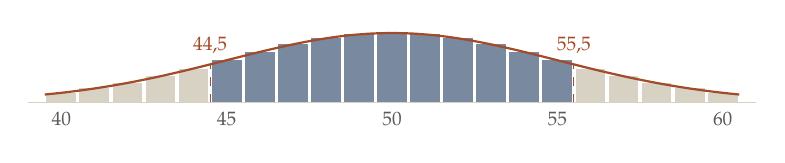
\begin{tikzpicture}[x=0.42cm,y=11cm]
\foreach \k in {40,...,60} {\pgfmathsetmacro{\h}{exp(-(\k-50)^2/50)/sqrt(50*pi)}
  \ifnum\k>44 \ifnum\k<56 \fill[tief!60] (\k-50-0.45,0) rectangle (\k-50+0.45,\h); \else \fill[linie] (\k-50-0.45,0) rectangle (\k-50+0.45,\h); \fi \else \fill[linie] (\k-50-0.45,0) rectangle (\k-50+0.45,\h); \fi}
\draw[akzent,thick,domain=-10.5:10.5,samples=100,smooth] plot (\x,{exp(-\x*\x/50)/sqrt(50*pi)});
\draw[akzent,dashed] (-5.5,0)--(-5.5,0.045) node[above,font=\scriptsize] {$44{,}5$}; \draw[akzent,dashed] (5.5,0)--(5.5,0.045) node[above,font=\scriptsize] {$55{,}5$};
\draw[linie] (-11,0)--(11,0); \foreach \k in {40,45,50,55,60} {\node[below,font=\scriptsize,grau] at (\k-50,0) {\k};}
\end{tikzpicture}
\end{center}
\probe{Symmetrie: $P(X\le44) = P(X\ge56) = \frac{1 - 0{,}7287}2 = 0{,}1356$; Normalnäherung $\Phi(-1{,}1) = 0{,}1357$. \checkmark}
\begin{mitnehmen}\kastentext
Die Stetigkeitskorrektur ersetzt ganzzahlige Grenzen $a\le X\le b$ durch $a - \frac12\le X\le b + \frac12$. Sie kostet nichts und verbessert die Näherung um eine Größenordnung --- besonders bei kleinem $\sigma$. Faustregel für die Anwendbarkeit: $np(1 - p)\ge9$; hier $25$.
\end{mitnehmen}
\end{loesungkarte}

%%%%%%%%%% 4.33
\stupserzwei{gruen}{$32 + 1{,}645\cdot5{,}43 = 40{,}9$; $32 + 2{,}326\cdot5{,}43 = 44{,}6$. Also: ab $41$ erhöht, ab $45$ auffällig.}{22pt}
\begin{loesungkarte}{gruen}{4.33}{Wann wird man stutzig?}
\derweg{Normalnäherung der Binomialverteilung; einseitige Schranken bei $95\,\%$ und $99\,\%$; dann das Problem, wenn viele gleichzeitig geprüft werden.}
\schritt{Modell}
$X\sim\operatorname{Bin}(400;\ 0{,}08)$, $\mu = 32$, $\sigma = \sqrt{400\cdot0{,}08\cdot0{,}92} = \sqrt{29{,}44} = 5{,}43$. $np(1 - p) = 29{,}4\ge9$: Normalnäherung zulässig.
\schritt{Schranken}
Einseitig (nur zu viele Komplikationen interessieren): $95\,\%$-Schranke $\mu + 1{,}645\sigma = 40{,}9$, $99\,\%$-Schranke $\mu + 2{,}326\sigma = 44{,}6$. Mit Stetigkeitskorrektur: $P(X\ge45)\approx1 - \Phi\bigl(\frac{44{,}5 - 32}{5{,}43}\bigr) = 1 - \Phi(2{,}30) = 0{,}011$; exakt $0{,}0106$.
\schritt{Deutung}
Bis $40$: unauffällig. $41$ bis $44$: erhöht --- aber bei unveränderter Qualität in etwa jedem zwanzigsten Jahr zu erwarten. Ab $45$: auffällig, etwa einmal in hundert Jahren durch Zufall.
\schritt{Multiples Testen}
Prüft man $1900$ Krankenhäuser mit der $99\,\%$-Schranke, erwartet man $19$ falsche Alarme pro Jahr --- bei lauter einwandfreien Häusern. Die Schranke muss dann strenger sein (Bonferroni: Niveau $\frac{0{,}01}{1900}$, Schranke $\mu + 4{,}4\sigma\approx56$), oder man kontrolliert den Anteil falscher Alarme statt der Wahrscheinlichkeit eines einzigen (False Discovery Rate).
\probe{Exakt $P(X\ge41) = 0{,}0625$, Näherung $1 - \Phi\bigl(\frac{40{,}5 - 32}{5{,}43}\bigr) = 1 - \Phi(1{,}57) = 0{,}058$. \checkmark}
\begin{mitnehmen}\kastentext
Eine Kontrollgrenze ist eine Aussage über \emph{ein} Krankenhaus in \emph{einem} Jahr. Wer viele prüft oder lange beobachtet, muss die Grenze anheben --- sonst findet er Auffälligkeiten, die nur die Zahl der Prüfungen widerspiegeln. Das ist die statistische Seite jeder Qualitätsüberwachung.
\end{mitnehmen}
\end{loesungkarte}

%%%%%%%%%% 4.34
\stupserzwei{tief}{Aus $E_1$ führt eine Nicht-Sechs zurück nach $E_0$, nicht nach $E_1$: Die Sechs ist verloren. Das ist der Grund, warum $42$ und nicht $36$ herauskommt.}{22pt}
\begin{loesungkarte}{tief}{4.34}{Zwei Sechsen hintereinander}
\derweg{Zustände nach einem Wurf beschreiben und für jeden eine Gleichung für die restliche Wartezeit aufstellen.}
\schritt{(a) --- bis zur ersten Sechs}
Sei $E$ die mittlere Zahl der Würfe. Ein Wurf; mit $\frac16$ fertig, mit $\frac56$ wieder am Anfang: $E = 1 + \frac56E$, also $E = 6$.
\schritt{(b), (c) --- zwei Zustände}
\begin{center}
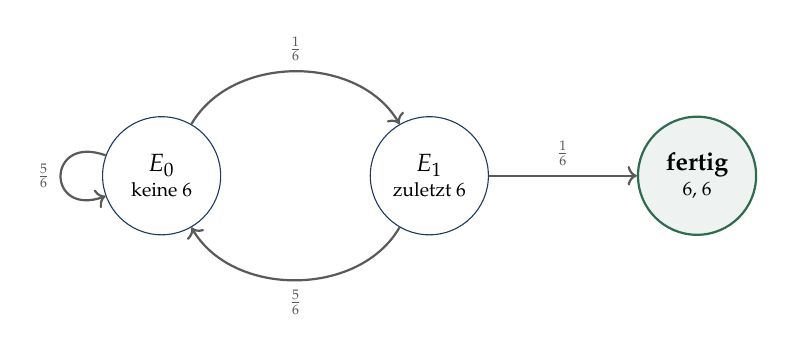
\begin{tikzpicture}[font=\small,node distance=3.4cm,
  zst/.style={draw=tief,circle,minimum size=1.5cm,align=center,fill=white},
  pf/.style={->,thick,grau}]
\node[zst] (z0) {$E_0$\\[-2pt]{\scriptsize keine 6}};
\node[zst,right of=z0] (z1) {$E_1$\\[-2pt]{\scriptsize zuletzt 6}};
\node[draw=gruen,thick,circle,minimum size=1.5cm,right of=z1,align=center,fill=gruen!8] (zz) {\textbf{fertig}\\[-2pt]{\scriptsize 6, 6}};
\draw[pf] (z0) to[out=60,in=120] node[above,font=\scriptsize]{$\frac16$} (z1);
\draw[pf] (z1) to[out=-120,in=-60] node[below,font=\scriptsize]{$\frac56$} (z0);
\draw[pf] (z1) -- node[above,font=\scriptsize]{$\frac16$} (zz);
\draw[pf] (z0) to[out=160,in=200,looseness=4] node[left,font=\scriptsize]{$\frac56$} (z0);
\end{tikzpicture}
\end{center}
Aus $E_0$: ein Wurf, dann mit $\frac16$ nach $E_1$, mit $\frac56$ zurück. Aus $E_1$: ein Wurf, mit $\frac16$ fertig, mit $\frac56$ zurück nach $E_0$.
\[ E_0 = 1 + \tfrac56E_0 + \tfrac16E_1,\qquad E_1 = 1 + \tfrac56E_0 . \]
Die erste gibt $E_0 = 6 + E_1$; einsetzen: $E_1 = 1 + \frac56(6 + E_1) = 6 + \frac56E_1$, also $E_1 = 36$ und $E_0 = 42$.
\schritt{(d) --- Grenzfall Münze}
$p = \frac12$: $E_0 = 2 + E_1$, $E_1 = 1 + \frac12(2 + E_1) = 2 + \frac12E_1$, also $E_1 = 4$, $E_0 = 6$. Sechs Münzwürfe bis zweimal Kopf hintereinander --- plausibel: In vier Würfen gelingt es etwa jedes zweite Mal.
\probe{Allgemein $E_0 = \frac1p + \frac1{p^{2}}$: $6 + 36 = 42$ und $2 + 4 = 6$. \checkmark\ Warum nicht $36 = 6\cdot6$? Weil eine Sechs ohne Nachfolgerin nichts nützt --- man beginnt von vorn, und das kostet im Mittel die $6$ Würfe extra.}
\begin{mitnehmen}\kastentext
Wartezeiten rechnet man mit Zuständen: Was ist nach einem Schritt passiert, und wo stehe ich dann? Die Reihe, die man sonst summieren müsste, steckt in der Unbekannten. Das ist die Methode des ersten Schritts --- dieselbe wie beim Ruinproblem (Aufgabe 4.37).
\end{mitnehmen}
\end{loesungkarte}

%%%%%%%%%% 4.35
\stupserzwei{gruen}{Nach zwei Wochen: $(0{,}4;\ 0{,}5;\ 0{,}1)\cdot P = (0{,}36 + 0{,}20 + 0{,}01;\ \dots)$.}{22pt}
\begin{loesungkarte}{gruen}{4.35}{Ein Patient in zwei Wochen}
\derweg{Zeilenvektor mal Matrix, zweimal.}
\schritt{Prüfen}
Zeilensummen von $P$: $1$, $1$, $1$. \checkmark\ Stochastische Matrix.
\schritt{Eine Woche}
$\pi_0 = (0, 1, 0)$. $\pi_1 = \pi_0P$ = zweite Zeile $= (0{,}40;\ 0{,}50;\ 0{,}10)$.
\schritt{Zwei Wochen}
$\pi_2 = \pi_1P$: G: $0{,}4\cdot0{,}9 + 0{,}5\cdot0{,}4 + 0{,}1\cdot0{,}1 = 0{,}36 + 0{,}20 + 0{,}01 = 0{,}57$. L: $0{,}4\cdot0{,}08 + 0{,}5\cdot0{,}5 + 0{,}1\cdot0{,}3 = 0{,}032 + 0{,}25 + 0{,}03 = 0{,}312$. S: $0{,}4\cdot0{,}02 + 0{,}5\cdot0{,}1 + 0{,}1\cdot0{,}6 = 0{,}008 + 0{,}05 + 0{,}06 = 0{,}118$. \\
$\pi_2 = (0{,}570;\ 0{,}312;\ 0{,}118)$: In zwei Wochen ist der Patient mit $57\,\%$ gesund, $31\,\%$ leicht und $12\,\%$ schwer erkrankt.
\probe{$0{,}570 + 0{,}312 + 0{,}118 = 1{,}000$. \checkmark\ Plausibel: Von L aus zieht es stark nach G ($0{,}4$ pro Woche), und G ist klebrig ($0{,}9$).}
\begin{mitnehmen}\kastentext
$\pi_n = \pi_0P^{n}$: Die Verteilung nach $n$ Schritten ist Zeilenvektor mal $n$-te Potenz. Das Eintragsmuster von $P^{n}$ nähert sich der stationären Verteilung in allen Zeilen (Aufgabe 4.36) --- die Kette vergisst, wo sie angefangen hat.
\end{mitnehmen}
\end{loesungkarte}

%%%%%%%%%% 4.36
\stupserzwei{gruen}{Aus (I): $0{,}1\pi_G = 0{,}4\pi_L + 0{,}1\pi_S$. Aus (III): $0{,}4\pi_S = 0{,}02\pi_G + 0{,}1\pi_L$. Zwei Gleichungen, dann normieren.}{22pt}
\begin{loesungkarte}{gruen}{4.36}{Die stationäre Verteilung}
\derweg{$\pi P = \pi$ als Bilanzgleichungen (Zufluss gleich Abfluss), zwei davon plus Normierung.}
\schritt{Gleichungen}
$\pi = (\pi_G, \pi_L, \pi_S)$ mit $\pi P = \pi$, spaltenweise:
(I) $0{,}9\pi_G + 0{,}4\pi_L + 0{,}1\pi_S = \pi_G$, also $0{,}4\pi_L + 0{,}1\pi_S = 0{,}1\pi_G$. \\
(III) $0{,}02\pi_G + 0{,}1\pi_L + 0{,}6\pi_S = \pi_S$, also $0{,}02\pi_G + 0{,}1\pi_L = 0{,}4\pi_S$. \\
(II) ist redundant; dafür (IV) $\pi_G + \pi_L + \pi_S = 1$.
\schritt{Lösen}
Aus (I): $\pi_G = 4\pi_L + \pi_S$. In (III): $0{,}08\pi_L + 0{,}02\pi_S + 0{,}1\pi_L = 0{,}4\pi_S$, also $0{,}18\pi_L = 0{,}38\pi_S$, $\pi_L = \frac{19}9\pi_S$. Dann $\pi_G = \frac{76}9\pi_S + \pi_S = \frac{85}9\pi_S$. Normierung: $\pi_S\bigl(\frac{85}9 + \frac{19}9 + 1\bigr) = \pi_S\cdot\frac{113}9 = 1$, $\pi_S = \frac9{113}$.
\[ \pi = \Bigl(\frac{85}{113}, \frac{19}{113}, \frac9{113}\Bigr) = (0{,}752;\ 0{,}168;\ 0{,}080). \]
\schritt{Deutung}
Langfristig ist der Patient $8\,\%$ der Zeit schwer krank. Mittlere Rückkehrzeit nach S: $\frac1{\pi_S} = \frac{113}9 = 12{,}6$ Wochen --- etwa alle drei Monate eine schwere Phase.
\probe{(II): $0{,}08\cdot0{,}752 + 0{,}5\cdot0{,}168 + 0{,}3\cdot0{,}080 = 0{,}0602 + 0{,}0841 + 0{,}0239 = 0{,}1682\approx\pi_L$. \checkmark\ Aufgabe 4.35 fortgesetzt: $\pi_2 = (0{,}57;\ 0{,}31;\ 0{,}12)$ ist schon auf dem Weg zu $(0{,}75;\ 0{,}17;\ 0{,}08)$. \checkmark}
\begin{mitnehmen}\kastentext
Stationäre Verteilung $=$ Linkseigenvektor zum Eigenwert $1$, normiert. Jede Gleichung ist eine Bilanz: Was pro Schritt in einen Zustand fließt, fließt auch heraus. Für irreduzible aperiodische Ketten ist sie eindeutig, und $\frac1{\pi_i}$ ist die mittlere Rückkehrzeit --- die Zahl, die man im Modell medizinisch deuten kann.
\end{mitnehmen}
\end{loesungkarte}

%%%%%%%%%% 4.37
\stupserzwei{gruen}{Mit $d_k = r_k - r_{k-1}$: $p\,d_{k+1} = q\,d_k$, also $d_k = (q/p)^{k-1}d_1$. Summieren von $r_0 = 1$ bis $r_N = 0$ bestimmt $d_1$.}{22pt}
\begin{loesungkarte}{gruen}{4.37}{Das Ruinproblem}
\derweg{Erster Schritt gibt eine Rekursion; die Differenzen sind geometrisch; Randbedingungen fixieren die Konstanten.}
\schritt{Rekursion}
$r_k$ = Ruinwahrscheinlichkeit bei Kapital $k$, $N = a + b$. Erster Schritt: $r_k = p\,r_{k+1} + q\,r_{k-1}$ für $1\le k\le N - 1$, mit $r_0 = 1$, $r_N = 0$ ($q = 1 - p$).
\schritt{Differenzen}
$(p + q)r_k = pr_{k+1} + qr_{k-1}\Rightarrow p(r_{k+1} - r_k) = q(r_k - r_{k-1})$. Mit $d_k = r_k - r_{k-1}$: $d_{k+1} = \frac qpd_k$, also $d_k = \rho^{k-1}d_1$ mit $\rho = \frac qp$.
\schritt{Fall $p\neq\frac12$}
$r_k - r_0 = \sum_{j=1}^{k}d_j = d_1\frac{1 - \rho^{k}}{1 - \rho}$. Aus $r_N = 0$: $d_1 = -\frac{1 - \rho}{1 - \rho^{N}}$. Also
\[ r_k = 1 - \frac{1 - \rho^{k}}{1 - \rho^{N}} = \frac{\rho^{k} - \rho^{N}}{1 - \rho^{N}},\qquad\text{Ruin bei Start } a\colon\ r_a = \frac{\rho^{a} - \rho^{a+b}}{1 - \rho^{a+b}}. \]
\schritt{Fall $p = \frac12$}
$\rho = 1$, $d_k = d_1$ konstant, $r_k = 1 + kd_1$, $r_N = 0\Rightarrow d_1 = -\frac1N$: $r_a = 1 - \frac aN = \frac b{a + b}$.
\schritt{Zahlen}
$a = 10$, $b = 90$. $p = \frac12$: $r = \frac{90}{100} = 90\,\%$. $p = 0{,}49$: $\rho = \frac{51}{49} = 1{,}0408$, $\rho^{10} = 1{,}492$, $\rho^{100} = 54{,}6$: $r = \frac{1{,}492 - 54{,}6}{1 - 54{,}6} = \frac{-53{,}1}{-53{,}6} = 99{,}1\,\%$. Ein Prozent Nachteil pro Runde macht aus $90\,\%$ Ruin $99\,\%$.
\probe{$p = \frac12$, $a = b$: $r = \frac12$ aus Symmetrie. \checkmark\ Formel für $p\neq\frac12$ bei $a = b = 50$, $p = 0{,}49$: $r = \frac{\rho^{50} - \rho^{100}}{1 - \rho^{100}} = 0{,}881$ --- bei gleichem Kapital verliert der Benachteiligte zu $88\,\%$. \checkmark}
\begin{mitnehmen}\kastentext
Gegen einen Gegner mit viel größerem Kapital ($b\to\infty$) ist der Ruin bei $p\le\frac12$ sicher und bei $p > \frac12$ gleich $\rho^{a}$. Das Casino hat beides: mehr Kapital und $p < \frac12$. Die Methode des ersten Schritts (Aufgabe 4.34) löst Wartezeiten und Treffwahrscheinlichkeiten von Irrfahrten gleichermaßen.
\end{mitnehmen}
\end{loesungkarte}

%%%%%%%%%% 4.38
\stupserzwei{gruen}{$E[S_T] = a$ und $S_T\in\{0, N\}$: $a = N\cdot P(S_T = N)$. Für die Dauer: $E[S_T^{2} - T] = a^{2}$, und $E[S_T^{2}] = N^{2}\cdot\frac aN = aN$.}{22pt}
\begin{loesungkarte}{gruen}{4.38}{Ruin mit dem Stoppsatz}
\derweg{Martingal, Stoppzeit, Voraussetzungen, Gleichung --- zweimal: mit $S_n$ für die Wahrscheinlichkeit, mit $S_n^{2} - n$ für die Dauer.}
\schritt{Martingal}
Für $p = \frac12$: $E[S_{n+1}\mid\mathcal F_n] = S_n + E[\xi_{n+1}] = S_n$. $S_n$ ist ein Martingal.
\schritt{Stoppzeit}
$T = \min\{n\colon S_n\in\{0, N\}\}$. Ob bis $n$ gestoppt wurde, hängt nur von $S_0, \dots, S_n$ ab. \checkmark\ Der gestoppte Prozess bleibt in $[0, N]$, also beschränkt; $T < \infty$ fast sicher (die Irrfahrt verlässt jedes endliche Intervall). Der Satz vom optionalen Stoppen ist anwendbar.
\schritt{Ruinwahrscheinlichkeit}
$E[S_T] = E[S_0] = a$. $S_T$ ist $0$ (Ruin) oder $N$ (Gewinn): $a = 0\cdot P(\text{Ruin}) + N\cdot P(\text{Gewinn})$, also $P(\text{Gewinn}) = \frac aN$, $P(\text{Ruin}) = \frac bN = \frac b{a + b}$. Wie in Aufgabe 4.37, in drei Zeilen.
\schritt{Spieldauer}
$M_n = S_n^{2} - n$ ist ein Martingal: $E[S_{n+1}^{2}\mid\mathcal F_n] = S_n^{2} + 2S_nE[\xi] + E[\xi^{2}] = S_n^{2} + 1$. Optionales Stoppen (mit $E[T] < \infty$): $E[S_T^{2}] - E[T] = a^{2}$. $E[S_T^{2}] = N^{2}\cdot\frac aN = aN$. Also $E[T] = aN - a^{2} = a(N - a) = ab$.
\probe{$a = 10$, $b = 90$: $900$ Runden im Mittel. $a = b = 1$: $E[T] = 1$ --- eine Runde entscheidet. \checkmark\ $a = b = 50$: $2500$ Runden; die Irrfahrt braucht $\sim d^{2}$ Schritte für Abstand $d$. \checkmark}
\begin{mitnehmen}\kastentext
Ein Martingal ist ein faires Spiel; der Stoppsatz sagt, dass keine Strategie es unfair macht --- unter Voraussetzungen (beschränkt oder integrierbar gestoppt), die bei der Verdopplungsstrategie gerade verletzt sind. $S_n^{2} - n$ als Martingal liefert die Dauer $ab$: Die symmetrische Irrfahrt braucht quadratisch viele Schritte.
\end{mitnehmen}
\end{loesungkarte}

%%%%%%%%%% 4.39
\stupserzwei{tief}{$1{,}96\sqrt{\frac{p(1 - p)}n}\le0{,}03\iff n\ge\bigl(\frac{1{,}96}{0{,}03}\bigr)^{2}p(1 - p) = 4268{,}4\cdot p(1 - p)$.}{22pt}
\begin{loesungkarte}{tief}{4.39}{Wie viele Patienten braucht die Studie?}
\derweg{Halbe Intervallbreite gleich Vorgabe setzen, nach $n$ auflösen, aufrunden.}
\schritt{(a)}
Halbe Breite $h = 1{,}96\sqrt{p(1 - p)/n}$. Nach $n$: $n = \frac{1{,}96^{2}p(1 - p)}{h^{2}}$. Ohne Vorwissen den ungünstigsten Fall $p(1 - p)\le\frac14$: $n = \frac{3{,}8416\cdot0{,}25}{0{,}0009} = 1067{,}1$, also $1068$ Patienten.
\schritt{(b)}
$p\approx0{,}1$: $p(1 - p) = 0{,}09$, $n = \frac{3{,}8416\cdot0{,}09}{0{,}0009} = 384{,}2$, also $385$. Weniger als die Hälfte --- Raten nahe $0$ oder $1$ sind leichter zu schätzen.
\schritt{(c)}
$h$ halbieren $\Rightarrow h^{2}$ vierteln $\Rightarrow n$ vervierfachen: $4270$ bzw.\ $1537$. Doppelte Genauigkeit, vierfacher Aufwand (Aufgabe 4.21).
\schritt{(d)}
Die Formel enthält nur $n$, nicht die Größe der Grundgesamtheit: Die Streuung von $\hat p$ hängt davon ab, wie viele man \emph{befragt}, nicht wie viele es \emph{gibt} --- solange ohne Zurücklegen aus einer großen Menge gezogen wird (Anteil $\frac n{\text{Gesamt}}$ klein). Eine Umfrage mit $1000$ Personen ist in Luxemburg so genau wie in China.
\probe{Aufgabe 4.42: $n = 250$, $\hat p = 0{,}64$: $h = 1{,}96\cdot0{,}0304 = 0{,}060$. Umgekehrt: für $h = 0{,}06$ und $p = 0{,}64$ braucht man $n = \frac{3{,}8416\cdot0{,}2304}{0{,}0036} = 246$. \checkmark}
\begin{mitnehmen}\kastentext
$n\approx\frac{4p(1 - p)}{h^{2}}$, im ungünstigsten Fall $\frac1{h^{2}}$: Für $\pm3\,\%$ braucht man gut $1000$, für $\pm1\,\%$ etwa $10\,000$. Diese Zahlen stehen hinter jeder Wahlumfrage --- und erklären, warum sie alle etwa $1000$ Befragte haben.
\end{mitnehmen}
\end{loesungkarte}

%%%%%%%%%% 4.40
\stupserzwei{akzent}{Alle vier Aussagen sind falsch. Der $p$-Wert bedingt auf $H_0$, nicht auf die Daten; er sagt nichts über Effektgröße oder Wiederholbarkeit.}{22pt}
\begin{loesungkarte}{akzent}{4.40}{Was der $p$-Wert nicht sagt}
\derweg{Die Definition hinschreiben und jede Aussage daran messen.}
\schritt{Definition}
$p = P(\text{Teststatistik mindestens so extrem wie beobachtet}\mid H_0)$. Eine Wahrscheinlichkeit \emph{über Daten}, berechnet \emph{unter der Annahme}, dass $H_0$ gilt.
\schritt{(a) falsch}
$P(H_0\mid\text{Daten})$ ist die umgekehrte Bedingung (Aufgabe 4.8). Sie zu berechnen bräuchte eine A-priori-Wahrscheinlichkeit für $H_0$ --- Bayes. Bei einer unplausiblen Hypothese (Prävalenz-Analogie: Aufgabe 4.10) kann $p = 0{,}03$ mit $P(H_0\mid\text{Daten}) > 50\,\%$ einhergehen.
\schritt{(b) falsch}
Dasselbe, mit $1 - p$. \enquote{Der Effekt ist real} ist eine Aussage über die Welt; der $p$-Wert ist eine Aussage über die Daten unter einer Annahme.
\schritt{(c) falsch}
Signifikanz misst, wie gut die Daten mit \enquote{kein Effekt} verträglich sind --- nicht, wie groß der Effekt ist. Mit $n = 100\,000$ ist jeder winzige Effekt signifikant; mit $n = 20$ auch ein großer oft nicht. Für Relevanz braucht man die Effektgröße mit Konfidenzintervall.
\schritt{(d) falsch}
Die Wiederholungswahrscheinlichkeit hängt von der (unbekannten) wahren Effektgröße ab --- das ist die Power. Bei $p = 0{,}03$ und typischer Power liegt die Chance auf erneute Signifikanz oft nur bei etwa $50\,\%$.
\schritt{(e) was er sagt}
$p = 0{,}03$: Wäre $H_0$ wahr, bekäme man so extreme Daten in $3\,\%$ der Studien. Das ist \emph{überraschend} unter $H_0$ --- mehr nicht. $p = 0{,}30$: so extreme Daten wären unter $H_0$ in $30\,\%$ der Studien zu erwarten --- nicht überraschend; das heißt \emph{nicht}, dass $H_0$ wahr ist (Abwesenheit von Evidenz ist nicht Evidenz der Abwesenheit).
\begin{fehler}\kastentext
Der $p$-Wert ist $P(\text{Daten}\mid H_0)$, gewünscht wird $P(H_0\mid\text{Daten})$. Das ist dieselbe Verwechslung wie Sensitivität gegen positiven Vorhersagewert. Und wie dort hängt die gewünschte Größe von einer \enquote{Prävalenz} ab --- hier: wie plausibel die Hypothese vorher war.
\end{fehler}
\begin{mitnehmen}\kastentext
Ein $p$-Wert ist ein Maß für Überraschung unter $H_0$, keine Wahrscheinlichkeit für Hypothesen, keine Effektgröße, keine Wiederholbarkeit. Berichten sollte man Effektgröße und Konfidenzintervall; der $p$-Wert ist davon eine verlustbehaftete Zusammenfassung.
\end{mitnehmen}
\end{loesungkarte}

%%%%%%%%%% 4.41
\stupserzwei{gruen}{$\ell'(p) = \frac kp - \frac{n - k}{1 - p} = 0\iff k(1 - p) = (n - k)p\iff p = \frac kn$.}{22pt}
\begin{loesungkarte}{gruen}{4.41}{Der Maximum-Likelihood-Schätzer}
\derweg{Log-Likelihood ableiten, Nullstelle, zweite Ableitung.}
\schritt{Likelihood}
$L(p) = \binom nkp^{k}(1 - p)^{n-k}$, $\ell(p) = \ln L = \text{const} + k\ln p + (n - k)\ln(1 - p)$.
\schritt{Maximum}
$\ell'(p) = \frac kp - \frac{n - k}{1 - p} = 0\iff k(1 - p) = (n - k)p\iff k = np\iff\hat p = \frac kn$.
\schritt{Zweite Ableitung}
$\ell''(p) = -\frac k{p^{2}} - \frac{n - k}{(1 - p)^{2}} < 0$ für $0 < k < n$: Maximum. (Randfälle $k = 0$ oder $k = n$: $\hat p = 0$ bzw.\ $1$, Maximum am Rand.)
\probe{Aufgabe 4.42: $\hat p = \frac{160}{250} = 0{,}64$. \checkmark\ $E[\hat p] = \frac{np}n = p$: erwartungstreu. $\operatorname{Var}\hat p = \frac{p(1 - p)}n$: Das ist das Quadrat des Standardfehlers aus Aufgabe 4.42. \checkmark}
\begin{mitnehmen}\kastentext
Maximum Likelihood liefert hier die relative Häufigkeit --- beruhigend. Bei anderen Modellen liefert es Schätzer, auf die man sonst nicht käme, und immer mit derselben Rezeptur: Likelihood, Logarithmus, Ableitung, Nullstelle. Die Krümmung $-\ell''(\hat p)$ (Fisher-Information) gibt zugleich die Genauigkeit.
\end{mitnehmen}
\end{loesungkarte}

%%%%%%%%%% 4.42
\stupserzwei{gruen}{$1{,}96\cdot0{,}0304 = 0{,}0595$: Intervall $[0{,}580;\ 0{,}700]$.}{22pt}
\begin{loesungkarte}{gruen}{4.42}{Ein Konfidenzintervall}
\derweg{Punktschätzer, Standardfehler, $\pm1{,}96$; dann die Deutung.}
\schritt{Rechnung}
$\hat p = \frac{160}{250} = 0{,}64$. $\mathrm{SE} = \sqrt{\frac{0{,}64\cdot0{,}36}{250}} = \sqrt{0{,}000922} = 0{,}0304$. Wald-Intervall: $0{,}64\pm1{,}96\cdot0{,}0304 = 0{,}64\pm0{,}060$, also $[0{,}580;\ 0{,}700]$.
\schritt{Was es bedeutet}
Das Verfahren \enquote{$\hat p\pm1{,}96\,\mathrm{SE}$} erzeugt in $95\,\%$ aller Studien ein Intervall, das die wahre Rate enthält. Die Aussage gilt für das \emph{Verfahren} über viele Studien.
\schritt{Was es nicht bedeutet}
Nicht: \enquote{Die wahre Rate liegt mit $95\,\%$ in $[0{,}58;\ 0{,}70]$.} Die wahre Rate ist eine feste Zahl; sie liegt im Intervall oder nicht. Nicht: \enquote{$95\,\%$ der Patienten sprechen mit Rate zwischen $58$ und $70\,\%$ an.} Und nicht: \enquote{Eine Wiederholung liefert mit $95\,\%$ ein $\hat p$ im Intervall} (das wären etwa $83\,\%$).
\probe{Anwendbarkeit: $n\hat p = 160\ge10$, $n(1 - \hat p) = 90\ge10$. \checkmark\ Wilson-Intervall (genauer bei kleinem $n$): $[0{,}579;\ 0{,}697]$ --- praktisch dasselbe. \checkmark}
\begin{mitnehmen}\kastentext
Ein Konfidenzintervall sagt, welche wahren Werte mit den Daten verträglich sind, und seine Breite sagt, wie viel man gelernt hat. Es enthält den Test: $p_0 = 0{,}6$ liegt im Intervall, also wäre $H_0\colon p = 0{,}6$ auf dem $5\,\%$-Niveau (zweiseitig) nicht abzulehnen --- einseitig in Aufgabe 4.43 schon.
\end{mitnehmen}
\end{loesungkarte}

%%%%%%%%%% 4.43
\stupserzwei{gruen}{$z = \frac{136 - 120}{6{,}93} = 2{,}31 > 1{,}645$: $H_0$ ablehnen. $p$-Wert $1 - \Phi(2{,}31) = 0{,}010$.}{22pt}
\begin{loesungkarte}{gruen}{4.43}{Ein einseitiger Test}
\derweg{Hypothesen, Verteilung unter $H_0$, Teststatistik, kritischer Wert, Entscheidung, $p$-Wert.}
\schritt{Hypothesen}
$H_0\colon p\le0{,}60$ gegen $H_1\colon p > 0{,}60$. Einseitig, weil nur eine Verbesserung interessiert.
\schritt{Unter $H_0$}
Im Grenzfall $p_0 = 0{,}6$: $X\sim\operatorname{Bin}(200;\ 0{,}6)$, $\mu = 120$, $\sigma = \sqrt{200\cdot0{,}6\cdot0{,}4} = \sqrt{48} = 6{,}93$. Normalnäherung zulässig ($48\ge9$).
\schritt{Teststatistik und Entscheidung}
$z = \frac{136 - 120}{6{,}93} = 2{,}31$. Kritischer Wert einseitig bei $\alpha = 0{,}05$: $1{,}645$. Da $2{,}31 > 1{,}645$: $H_0$ ablehnen. Das Medikament hebt die Heilungsrate signifikant.
\schritt{$p$-Wert}
$P(X\ge136\mid p = 0{,}6)\approx1 - \Phi(2{,}31) = 0{,}010$; mit Stetigkeitskorrektur $1 - \Phi\bigl(\frac{135{,}5 - 120}{6{,}93}\bigr) = 1 - \Phi(2{,}24) = 0{,}013$. Exakt (Binomialsumme): $0{,}012$.
\probe{Mit dem Konfidenzintervall: $\hat p = 0{,}68$, $\mathrm{SE} = \sqrt{0{,}68\cdot0{,}32/200} = 0{,}033$, einseitige untere Grenze $0{,}68 - 1{,}645\cdot0{,}033 = 0{,}626 > 0{,}60$. \checkmark\ Zweiseitig wäre der kritische Wert $1{,}96$ --- auch dann abgelehnt, mit $p = 0{,}021$.}
\begin{mitnehmen}\kastentext
Einseitig testet man, wenn die Richtung \emph{vor} der Datenerhebung festgelegt ist --- nie nachträglich, weil die Daten in eine Richtung zeigen. Und Signifikanz ist nicht Relevanz (Aufgabe 4.40): $68\,\%$ statt $60\,\%$ ist der Effekt, das Konfidenzintervall $[0{,}62;\ 0{,}74]$ seine Unsicherheit, und erst der Vergleich mit Kosten und Nebenwirkungen die Entscheidung.
\end{mitnehmen}
\end{loesungkarte}

\cleardoublepage
\setgebiet{6}{Numerik}{mittel}
\chapter{Lösungen: Numerik}

%%%%%%%%%% 5.1
\stupserzwei{tief}{$0{,}1 = (0{,}0\overline{0011})_2$. Auf 52 Bit gerundet ist das $0{,}1000000000000000055\dots$ --- ein Hauch zu groß.}{22pt}
\begin{loesungkarte}{tief}{5.1}{Binär, Epsilon, $0{,}1 + 0{,}2$}
\derweg{Dualbrüche entwickeln, Rundung bei 52 Bit, dann Epsilon als Abstand zur nächsten darstellbaren Zahl.}
\schritt{(a)}
$0{,}1\cdot2 = 0{,}2\to0$; $0{,}4\to0$; $0{,}8\to0$; $1{,}6\to1$, Rest $0{,}6$; $1{,}2\to1$, Rest $0{,}2$ --- ab hier wiederholt sich alles: $0{,}1 = (0{,}0\,0011\,0011\,0011\dots)_2$. Ein Bruch $\frac pq$ (gekürzt) ist binär genau dann endlich, wenn $q$ eine Zweierpotenz ist; $10 = 2\cdot5$ hat den Faktor $5$.
\schritt{(b)}
Gespeichert werden $\operatorname{fl}(0{,}1) = 0{,}1 + 5{,}55\cdot10^{-18}$ und $\operatorname{fl}(0{,}2) = 0{,}2 + 1{,}11\cdot10^{-17}$. Ihre Summe $0{,}3 + 1{,}67\cdot10^{-17}$ wird auf die nächste double gerundet, und die ist $0{,}3000000000000000444$; die double zu \enquote{$0{,}3$} dagegen ist $0{,}2999999999999999889$. Die Ausgabe zeigt die kürzeste Dezimalzahl, die die gespeicherte double eindeutig bezeichnet: $0{,}30000000000000004$.
\schritt{(c)}
$\varepsilon_M$ ist der Abstand von $1$ zur nächstgrößeren darstellbaren Zahl; gleichbedeutend: der maximale relative Rundungsfehler ist $\varepsilon_M/2$. $1 + 10^{-16}$: Das liegt näher an $1$ als an $1 + \varepsilon_M$, Ergebnis $1$. $1 + 10^{-15}$: etwa $1 + 4{,}5\varepsilon_M$, gerundet auf $1 + 4\varepsilon_M$ oder $1 + 5\varepsilon_M$ --- ungleich $1$, aber nur auf $\pm11\,\%$ der Störung genau.
\schritt{(d)}
double: $\log_{10}2^{52}\approx15{,}7$, also $15$ bis $16$ Dezimalstellen. single: $\log_{10}2^{23}\approx6{,}9$, also $6$ bis $7$ Stellen.
\probe{$0{,}1 + 0{,}2 = 0{,}3$ liefert \texttt{False}; $0{,}1 + 0{,}2 - 0{,}3$ liefert $5{,}55\cdot10^{-17}$ --- ein Viertel von $\varepsilon_M$, genau der Rundungsrest. \checkmark}
\begin{mitnehmen}\kastentext
Dezimalbrüche sind im Rechner fast nie exakt; $\frac12, \frac14, 0{,}375$ sind es, $0{,}1$ nicht. Jede Rechnung trägt einen relativen Fehler bis $\frac{\varepsilon_M}2$ --- das ist das \emph{Standardmodell} der Gleitpunktarithmetik, und alles in Kapitel 1 und 2 folgt daraus.
\end{mitnehmen}
\end{loesungkarte}

%%%%%%%%%% 5.2
\stupserzwei{akzent}{(d) Kleine zuerst: $10^{4}\cdot10^{-16} = 10^{-12}$ wird exakt gebildet, dann $1 + 10^{-12}$ --- und das ist darstellbar.}{22pt}
\begin{loesungkarte}{akzent}{5.2}{Gleich ist nicht gleich}
\derweg{In jedem Fall fragen: Welche Zahl wird wann gerundet, und ist die Zwischensumme darstellbar?}
\schritt{(a)}
Bei $10^{16}\approx2^{53}$ ist der Abstand benachbarter doubles $2$. $10^{16} + 1$ wird zu $10^{16}$ gerundet, die Differenz ist $0$. Andersherum: $1 - 10^{16}$ ist exakt $-9\,999\,999\,999\,999\,999$ --- nicht darstellbar, gerundet zu $-10^{16}$; Summe wieder $0$. Beide Klammerungen geben $0$ statt $1$; mit $10^{15}$ statt $10^{16}$ gäbe die zweite das richtige Ergebnis, die erste nicht. Assoziativität ist verloren.
\schritt{(b)}
$(0{,}1 + 0{,}2) + 0{,}3 = 0{,}6000000000000001$, $0{,}1 + (0{,}2 + 0{,}3) = 0{,}6$. Verletzt ist das Assoziativgesetz: Jede Zwischensumme wird gerundet, und wo gerundet wird, hängt von der Klammerung ab.
\schritt{(c)}
$x = 0{,}1 + 0{,}1 + \dots$ trifft die $1$ nie exakt: Nach zehn Additionen steht $0{,}9999999999999999$ da. Richtig prüft man $|x - 1| < \text{tol}$ mit einer Toleranz --- absolut für Werte nahe $0$, sonst relativ: $|x - y|\le\text{tol}\cdot\max(|x|, |y|)$. Besser noch: Schleifen über ganze Zahlen zählen und $x = k/10$ berechnen.
\schritt{(d)}
Vorwärts: $1 + 10^{-16} = 1$, und das $10^{4}$-mal --- Ergebnis $1$. Kleine zuerst: $10^{4}\cdot10^{-16} = 10^{-12}$ (Summen kleiner Zahlen untereinander sind relativ genau), dann $1 + 10^{-12} = 1{,}000000000001$ --- richtig. Allgemein: aufsteigend nach Betrag summieren, oder paarweise (Baum), oder mit Kahan-Kompensation; alle drei halten die Zwischensummen in vergleichbarer Größe.
\begin{fehler}\kastentext
Gleitpunktzahlen sind kein Körper: nicht assoziativ, nicht distributiv, mit Lücken. \texttt{==} auf Gleitpunktzahlen ist fast immer ein Fehler; Gleichheit heißt \enquote{näher als eine Toleranz}. Und die Reihenfolge einer Summe ist Teil des Algorithmus.
\end{fehler}
\begin{mitnehmen}\kastentext
Zwei Faustregeln: Große Zahlen fressen kleine (Absorption), und fast gleiche Zahlen subtrahieren löscht Stellen aus (Auslöschung, Aufgaben 5.4, 5.5). Wer eine Rechnung plant, ordnet sie so, dass beides selten vorkommt.
\end{mitnehmen}
\end{loesungkarte}

%%%%%%%%%% 5.3
\stupserzwei{gruen}{Mantisse: die Bits nach dem Komma von $(1{,}1001)_2$, also $1001$ und dann $48$ Nullen. Exponentfeld $1025 = (10000000001)_2$.}{22pt}
\begin{loesungkarte}{gruen}{5.3}{$-6{,}25$ als double}
\derweg{Betrag binär, normalisieren, Exponent plus Bias, führende Eins weglassen.}
\schritt{Vorzeichen}
$x < 0$: $s = 1$.
\schritt{Binär}
$6 = (110)_2$, $0{,}25 = 2^{-2} = (0{,}01)_2$: $6{,}25 = (110{,}01)_2$.
\schritt{Normalisieren}
$(110{,}01)_2 = (1{,}1001)_2\cdot2^{2}$: Exponent $e = 2$, Exponentfeld $e + 1023 = 1025 = (10000000001)_2$.
\schritt{Mantisse}
Die führende $1$ ist implizit; gespeichert wird $1001\,0000\dots0$ (52 Bit).
\schritt{Ergebnis}
$1\ |\ 10000000001\ |\ 1001000\dots0$; hexadezimal \texttt{C019 0000 0000 0000}.
\probe{Rückwärts: $(-1)^{1}\cdot(1 + \frac12 + \frac1{16})\cdot2^{1025 - 1023} = -1{,}5625\cdot4 = -6{,}25$. \checkmark\ Hex: $\mathtt C = 1100$ (Vorzeichen $1$, Exponent beginnt $100$), $\mathtt 0 = 0000$, $\mathtt 1 = 0001$ (Exponent endet $\dots0001$), $\mathtt 9 = 1001$ (Mantissenanfang). \checkmark}
\begin{mitnehmen}\kastentext
double: $1 + 11 + 52$ Bit, Bias $1023$, implizite Eins --- also $53$ Bit Genauigkeit und Exponenten von $-1022$ bis $1023$ (Zahlen bis etwa $1{,}8\cdot10^{308}$). Sonderfälle: Exponentfeld $0$ für $0$ und denormalisierte Zahlen, $2047$ für $\pm\infty$ und NaN.
\end{mitnehmen}
\end{loesungkarte}

%%%%%%%%%% 5.4
\stupserzwei{gruen}{$\sqrt{10^{16} - 4} = 10^{8}\sqrt{1 - 4\cdot10^{-16}}\approx10^{8}(1 - 2\cdot10^{-16})$; die Differenz zu $10^{8}$ ist $2\cdot10^{-8}$, aber double hat bei $10^{8}$ nur eine Auflösung von $1{,}5\cdot10^{-8}$.}{22pt}
\begin{loesungkarte}{gruen}{5.4}{Die Mitternachtsformel versagt}
\derweg{Die kleine Nullstelle entsteht als Differenz fast gleicher Zahlen; stattdessen die große berechnen und Vieta benutzen.}
\schritt{Exakt}
$x_{1,2} = \frac{10^{8}\pm\sqrt{10^{16} - 4}}2$. Exakt: $x_1 = 99\,999\,999{,}99999999$, $x_2 = 1{,}0000000000000001\cdot10^{-8}$ (Vieta: $x_1x_2 = 1$).
\schritt{Was der Rechner tut}
$\sqrt{10^{16} - 4}$ wird in double zu $10^{8}$ gerundet (der Unterschied $2\cdot10^{-8}$ liegt unter dem Zahlenabstand $1{,}49\cdot10^{-8}$ bei $10^{8}$ --- genauer: $10^{16} - 4$ selbst ist schon nicht darstellbar und wird $10^{16}$). Dann $x_2 = \frac{10^{8} - 10^{8}}2 = 0$, oder bei etwas anderer Rundung $7{,}45\cdot10^{-9}$ --- $25\,\%$ daneben. Auslöschung: Zwei $16$-stellige Zahlen, die in $16$ Stellen übereinstimmen, haben eine Differenz ohne gültige Stelle.
\schritt{Abhilfe}
Die Nullstelle ohne Auslöschung zuerst: $x_1 = \frac{10^{8} + \sqrt{\dots}}2 = 10^{8}$ (richtig auf $16$ Stellen). Dann $x_2 = \frac q{x_1} = 10^{-8}$ (Vieta, eine Division, kein Fehler). Allgemein: $x_1 = \frac{-p - \operatorname{sgn}(p)\sqrt{p^{2} - 4q}}2$, $x_2 = \frac q{x_1}$.
\probe{$x_1x_2 = 10^{8}\cdot10^{-8} = 1 = q$, $x_1 + x_2 = 10^{8} = -p$. \checkmark}
\begin{mitnehmen}\kastentext
Auslöschung ist nicht der Rundungsfehler --- der ist winzig. Sie ist die Verstärkung eines winzigen Fehlers durch eine Subtraktion fast gleicher Zahlen: Das Ergebnis ist klein, der absolute Fehler bleibt, der relative explodiert. Gegenmittel sind immer algebraisch: umformen, bevor man rechnet.
\end{mitnehmen}
\end{loesungkarte}

%%%%%%%%%% 5.5
\stupserzwei{gruen}{$\frac{2\sin^{2}(x/2)}{x^{2}}$: Für $x = 10^{-8}$ ist $\sin(5\cdot10^{-9}) = 5\cdot10^{-9}$ auf $16$ Stellen, das Quadrat $2{,}5\cdot10^{-17}$, mal $2$ durch $10^{-16}$: $0{,}5$.}{22pt}
\begin{loesungkarte}{gruen}{5.5}{$\frac{1 - \cos x}{x^{2}}$ für kleines $x$}
\derweg{Wahren Wert mit Taylor; dann sehen, dass $\cos x$ auf $1$ gerundet wird; Identität oder Reihe als Ausweg.}
\schritt{Wahrer Wert}
$\cos x = 1 - \frac{x^{2}}2 + \frac{x^{4}}{24} - \dots$, also $\frac{1 - \cos x}{x^{2}} = \frac12 - \frac{x^{2}}{24} + \dots$ Für $x = 10^{-8}$: $0{,}5$ bis auf $4\cdot10^{-18}$.
\schritt{Was der Rechner tut}
$\cos(10^{-8}) = 1 - 5\cdot10^{-17}$. Die nächste double unter $1$ ist $1 - 1{,}1\cdot10^{-16}$; also $\operatorname{fl}(\cos x) = 1$. Dann $1 - 1 = 0$, geteilt durch $10^{-16}$: $0$. Auslöschung in Reinform: Die Information über $\frac{x^{2}}2$ war nie im gespeicherten Kosinus.
\schritt{Abhilfe 1: Identität}
$1 - \cos x = 2\sin^{2}\frac x2$, also $\frac{1 - \cos x}{x^{2}} = \frac12\Bigl(\frac{\sin(x/2)}{x/2}\Bigr)^{2}$. Keine Subtraktion; $\sin(5\cdot10^{-9})$ ist relativ genau, das Ergebnis $0{,}5$ auf $16$ Stellen.
\schritt{Abhilfe 2: Reihe}
Für $|x| < 10^{-4}$ reicht $\frac12 - \frac{x^{2}}{24}$ (Fehler $< x^{4}/720 < 10^{-19}$); für größere $x$ die Originalformel. Bibliotheken tun genau das: Fallunterscheidung nach $|x|$.
\probe{$x = 10^{-3}$: Original $\frac{1 - 0{,}99999950000004}{10^{-6}} = 0{,}49999996$ (stimmt auf $8$ Stellen, $8$ verloren). Identität: $0{,}4999999583333$ (alle Stellen). \checkmark}
\begin{mitnehmen}\kastentext
Funktionen wie $1 - \cos x$, $e^{x} - 1$, $\ln(1 + x)$, $\sqrt{1 + x} - 1$ für kleines $x$ sind die klassischen Auslöschungsfallen; jede Bibliothek hat dafür eigene Routinen (\texttt{expm1}, \texttt{log1p}). Wer die Taylorreihe kennt, sieht die Gefahr: Das Ergebnis ist $O(x^{2})$, die Summanden sind $O(1)$.
\end{mitnehmen}
\end{loesungkarte}

%%%%%%%%%% 5.6
\stupserzwei{gruen}{Ab $S\approx10^{6}\approx2^{20}$ ist der Abstand benachbarter single-Zahlen $2^{20}\cdot2^{-23} = 0{,}125$. Addiert man $0{,}1$, wird das Ergebnis auf $S + 0{,}125$ gerundet: jeder Schritt $25\,\%$ zu viel.}{22pt}
\begin{loesungkarte}{gruen}{5.6}{Zehn Millionen mal $0{,}1$}
\derweg{Schranke aus dem Standardmodell; dann den tatsächlichen Mechanismus ansehen --- der ist spezifischer und erklärt das Vorzeichen.}
\schritt{Exakt}
$10^{7}\cdot0{,}1 = 10^{6}$.
\schritt{Schranke}
Jede Addition: $S_k = (S_{k-1} + x_k)(1 + \delta_k)$, $|\delta_k|\le\varepsilon_M$. Ausmultipliziert: $|S_n - \sum x_i|\le(n - 1)\varepsilon_M\sum|x_i|$. Mit $\varepsilon_M = 6\cdot10^{-8}$ und $\sum|x_i| = 10^{6}$: bis zu $0{,}6\cdot10^{6}$ --- $60\,\%$. Die Schranke ist pessimistisch, aber sie warnt: lineares Wachstum in $n$.
\schritt{Tatsächlich}
Das Programm liefert $1\,087\,937$ --- $8{,}8\,\%$ zu viel. Der Mechanismus: Sobald $S > 2^{20}\approx10^{6}$ ist, beträgt der Zahlenabstand $0{,}125$; $S + 0{,}1$ wird zu $S + 0{,}125$ gerundet, also systematisch $25\,\%$ zu viel pro Schritt. Schon ab $S > 2^{19}$ ist der Abstand $0{,}0625$ und $0{,}1$ wird mal zu $0{,}0625$, mal zu $0{,}125$ gerundet. Bei $S > 2^{24} = 1{,}7\cdot10^{7}$ wäre $S + 0{,}1 = S$: Die Summe bliebe stehen.
\schritt{Besser}
Kahan-Summation (den Rundungsrest mitführen): Fehler $O(\varepsilon_M)$ statt $O(n\varepsilon_M)$. Paarweise Summation: $O(\varepsilon_M\log n)$. Oder einfach double: $\varepsilon_M = 10^{-16}$, Fehler bei $10^{7}$ Additionen etwa $10^{-9}$ relativ. Oder gar nicht summieren: $n\cdot0{,}1$.
\probe{Rechnung mit dem Mechanismus: In der Phase $S\in[2^{20}, 1{,}09\cdot10^{6}]$ gewinnt jeder Schritt $0{,}025$ extra; das sind etwa $(1{,}09\cdot10^{6} - 1{,}05\cdot10^{6})/0{,}125\approx3\cdot10^{5}$ Schritte, Zuwachs $8000$ --- plus die Phase davor. Größenordnung $10^{4}$ bis $10^{5}$; tatsächlich $8{,}8\cdot10^{4}$. \checkmark}
\begin{mitnehmen}\kastentext
Rundungsfehler sind nicht zufällig: Bei $0{,}1$ in single sind sie systematisch positiv, und die Summe läuft davon. Die Schranke $n\varepsilon_M$ sagt, \emph{dass} man bei $10^{7}$ Summanden in single nichts mehr erwarten darf; der Mechanismus sagt, \emph{wie} es schiefgeht.
\end{mitnehmen}
\end{loesungkarte}

%%%%%%%%%% 5.7
\stupserzwei{tief}{$\ln$: $\kappa = \bigl|\frac{x\cdot1/x}{\ln x}\bigr| = \frac1{|\ln x|}$ --- unendlich bei $x = 1$. Subtraktion: $\kappa = \frac{|x|}{|x - y|}$ --- unendlich bei $x = y$.}{22pt}
\begin{loesungkarte}{tief}{5.7}{Die Kondition elementarer Funktionen}
\derweg{$\kappa = |xf'/f|$ ausrechnen und die Nullstellen des Nenners suchen.}
\schritt{(a)}
$\sqrt x$: $\kappa = \bigl|\frac{x\cdot\frac1{2\sqrt x}}{\sqrt x}\bigr| = \frac12$ --- überall gut, halbiert sogar den relativen Fehler. \\
$e^{x}$: $\kappa = \bigl|\frac{xe^{x}}{e^{x}}\bigr| = |x|$ --- schlecht für großes $|x|$: $e^{100}$ mit $x$ auf $16$ Stellen hat nur $14$ richtige. \\
$\ln x$: $\kappa = \frac1{|\ln x|}$ --- schlecht nahe $x = 1$, wo $\ln x\approx0$ (deshalb \texttt{log1p}).
\schritt{(b)}
$\sin x$: $\kappa = |x\cot x|$ --- unendlich bei $x = k\pi$, $k\neq0$ (Nullstellen), und wachsend für großes $|x|$: $\sin(10^{10})$ ist aus einer $16$-stelligen Eingabe nicht mehr bestimmbar, weil $10^{10}$ nur auf $\pm10^{-6}$ bekannt ist und das schon ein Teil der Periode ist.
\schritt{(c)}
$f(x) = x - y$: $\kappa_x = \bigl|\frac{x\cdot1}{x - y}\bigr| = \frac{|x|}{|x - y|}$. Für $x\approx y$ beliebig groß: Das ist die Auslöschung, als Konditionszahl ausgedrückt. (Für $x + y$ mit gleichem Vorzeichen ist $\kappa_x = \frac{|x|}{|x + y|}\le1$: Addition gleicher Vorzeichen ist harmlos.)
\schritt{(d)}
Nur $\sqrt x$ (und Multiplikation, Division: $\kappa = 1$). Die Subtraktion ist die einzige Grundrechenart, deren Kondition unbeschränkt ist --- und sie steckt in jeder Differenz, jedem Differenzenquotienten, jeder Mitternachtsformel.
\probe{$e^{x}$ bei $x = 10$: $\kappa = 10$. $x = 10(1 + 10^{-16})$ gibt $e^{x} = e^{10}(1 + 10^{-15})$ --- Faktor $10$. \checkmark}
\begin{mitnehmen}\kastentext
Kondition ist eine Eigenschaft des Problems: Kein Algorithmus kann $\ln(1{,}000000001)$ aus einer $16$-stelligen Eingabe auf mehr als $7$ Stellen bestimmen. Was ein Algorithmus kann, ist, \emph{keinen zusätzlichen} Fehler zu machen --- das ist Stabilität (Aufgabe 5.10).
\end{mitnehmen}
\end{loesungkarte}

%%%%%%%%%% 5.8
\stupserzwei{gruen}{$\kappa = \bigl|\frac{c}{x_1}\frac{dx_1}{dc}\bigr| = \frac{1 - \delta^{2}}{(1 + \delta)\,2\delta}\approx\frac1{2\delta}$.}{22pt}
\begin{loesungkarte}{gruen}{5.8}{Kondition einer doppelten Nullstelle}
\derweg{Nullstelle als Funktion des Koeffizienten, ableiten, relative Kondition bilden.}
\schritt{Nullstellen}
$x_{1,2} = 1\pm\sqrt{1 - (1 - \delta^{2})} = 1\pm\delta$. Für $\delta\to0$ fallen sie zusammen.
\schritt{Als Funktion von $c$}
$c = 1 - \delta^{2}$, $x_1(c) = 1 + \sqrt{1 - c}$, $\frac{dx_1}{dc} = -\frac1{2\sqrt{1 - c}} = -\frac1{2\delta}$.
\schritt{Kondition}
$\kappa = \Bigl|\frac{c\,x_1'(c)}{x_1(c)}\Bigr| = \frac{1 - \delta^{2}}{2\delta(1 + \delta)} = \frac{1 - \delta}{2\delta}\approx\frac1{2\delta}$.
\schritt{Deutung}
Für $\delta = 10^{-4}$ ist $\kappa = 5000$: Eine Störung des Koeffizienten um $10^{-16}$ (eine Rundung) verschiebt die Nullstelle relativ um $5\cdot10^{-13}$. Für $\delta = 10^{-8}$: $\kappa = 5\cdot10^{7}$, und die Nullstellen sind nur noch auf $8$ Stellen bestimmt. Bei $\delta = 0$ (doppelte Nullstelle) ist $\kappa = \infty$: Eine Störung $\varepsilon$ des Koeffizienten verschiebt die Nullstelle um $\sqrt\varepsilon$, nicht um $\varepsilon$ --- die Ableitung existiert nicht.
\probe{$\delta = 0$, $c\to1 - \varepsilon$: Nullstellen $1\pm\sqrt\varepsilon$. Mit $\varepsilon = 10^{-16}$: $1\pm10^{-8}$ --- acht Stellen verloren. \checkmark}
\begin{mitnehmen}\kastentext
Mehrfache und nahe Nullstellen sind schlecht konditioniert, unabhängig vom Verfahren. Das berühmte Wilkinson-Polynom $\prod(x - k)$, $k = 1, \dots, 20$, hat einfache Nullstellen, aber Konditionszahlen bis $10^{13}$: Nullstellen aus Koeffizienten zu berechnen ist grundsätzlich heikel.
\end{mitnehmen}
\end{loesungkarte}

%%%%%%%%%% 5.9
\stupserzwei{gruen}{$\|A\|_\infty = 2{,}0001$, $\|A^{-1}\|_\infty = \frac{1{,}0001 + 1}{0{,}0001} = 20\,001$, Produkt $40\,004$.}{22pt}
\begin{loesungkarte}{gruen}{5.9}{Eine Konditionszahl von $40\,000$}
\derweg{Zweimal lösen, Änderungen vergleichen, Konditionszahl als Zeilensummennormen.}
\schritt{(a)}
$Z_2 - Z_1$: $0{,}0001x_2 = 0{,}0001$, $x_2 = 1$, $x_1 = 1$. $x = (1, 1)$.
\schritt{(b)}
$Z_2 - Z_1$: $0{,}0001x_2 = 0{,}0002$, $x_2 = 2$, $x_1 = 0$. $\tilde x = (0, 2)$. Die rechte Seite änderte sich um $10^{-4}$, die Lösung um $1$ in jeder Komponente.
\schritt{(c)}
$\|A\|_\infty = \max(2;\ 2{,}0001) = 2{,}0001$. $A^{-1} = \frac1{0{,}0001}\begin{pmatrix}1{,}0001 & -1\\ -1 & 1\end{pmatrix}$, $\|A^{-1}\|_\infty = \frac{2{,}0001}{0{,}0001} = 20\,001$. $\operatorname{cond}_\infty(A) = 2{,}0001\cdot20\,001 = 40\,004$. \\
Störungsabschätzung: $\frac{\|\Delta x\|_\infty}{\|x\|_\infty} = \frac11 = 1$; rechte Seite $\operatorname{cond}\cdot\frac{\|\Delta b\|_\infty}{\|b\|_\infty} = 40\,004\cdot\frac{0{,}0001}{2{,}0001} = 2{,}0$. $1\le2$: Die Abschätzung gilt und ist bis auf den Faktor $2$ scharf.
\probe{Geometrisch: Zwei fast parallele Geraden ($x_1 + x_2 = 2$ und $x_1 + 1{,}0001x_2 = 2{,}0001$); ihr Schnittpunkt wandert weit, wenn man eine Gerade minimal verschiebt. \checkmark}
\begin{mitnehmen}\kastentext
$\operatorname{cond}(A)\approx10^{k}$ heißt: bis zu $k$ Stellen gehen verloren, egal wie gut der Löser ist. Bei $\operatorname{cond} = 4\cdot10^{4}$ und $\varepsilon_M = 10^{-16}$ bleiben $11$ Stellen; bei $\operatorname{cond} = 10^{16}$ keine. Deshalb berechnet jeder gute Löser eine Schätzung der Konditionszahl mit.
\end{mitnehmen}
\end{loesungkarte}

%%%%%%%%%% 5.10
\stupserzwei{gruen}{$(1 + \delta_i)(1 + \eta_i)\cdots(1 + \eta_n) = 1 + \theta_i$ mit $|\theta_i|\le(n - i + 2)\varepsilon_M + O(\varepsilon_M^{2})$ --- höchstens $n$ Faktoren.}{22pt}
\begin{loesungkarte}{gruen}{5.10}{Das Skalarprodukt ist rückwärtsstabil}
\derweg{Jede Rundung als Faktor $(1 + \delta)$; alle Faktoren, die ein Produkt $x_iy_i$ treffen, zu einem $(1 + \theta_i)$ zusammenfassen; $\theta_i$ auf $x_i$ abwälzen.}
\schritt{Standardmodell}
$\operatorname{fl}(x_iy_i) = x_iy_i(1 + \delta_i)$, $|\delta_i|\le\varepsilon_M$. Teilsummen: $s_1 = x_1y_1(1 + \delta_1)$, $s_k = \bigl(s_{k-1} + x_ky_k(1 + \delta_k)\bigr)(1 + \eta_k)$, $|\eta_k|\le\varepsilon_M$.
\schritt{Ausmultiplizieren}
Der Term $x_iy_i$ wird von $\delta_i$ und von allen $\eta_k$ mit $k\ge\max(i, 2)$ getroffen:
\[ \tilde s = \sum_{i=1}^{n}x_iy_i(1 + \delta_i)\prod_{k=\max(i,2)}^{n}(1 + \eta_k) =: \sum_{i=1}^{n}x_iy_i(1 + \theta_i). \]
\schritt{Abschätzen}
Ein Produkt von $m$ Faktoren $(1 + \epsilon_j)$ mit $|\epsilon_j|\le\varepsilon_M$ ist $1 + \theta$ mit $|\theta|\le m\varepsilon_M + O(\varepsilon_M^{2})$. Hier $m\le n$: $|\theta_i|\le n\varepsilon_M$.
\schritt{Rückwärts lesen}
$\tilde s = \sum\tilde x_iy_i$ mit $\tilde x_i = x_i(1 + \theta_i)$, $|\tilde x_i - x_i|\le n\varepsilon_M|x_i|$. Das berechnete Skalarprodukt ist das \emph{exakte} Skalarprodukt leicht gestörter Daten. $\blacksquare$
\probe{Vorwärts folgt daraus: $|\tilde s - s|\le n\varepsilon_M\sum|x_iy_i|$. Für $s\approx0$ bei großen $|x_iy_i|$ ist das relativ riesig --- aber das ist die Kondition des Problems, nicht die Schuld des Algorithmus. \checkmark}
\begin{mitnehmen}\kastentext
Rückwärtsstabil: Das Ergebnis ist exakt für gestörte Eingaben, Störung $O(\varepsilon_M)$. Dann gilt Fehler $\lesssim$ Kondition $\times$ $\varepsilon_M$ --- die Arbeitsteilung der Numerik: Der Algorithmus garantiert Stabilität, das Problem bestimmt die Kondition, das Produkt ist der Fehler.
\end{mitnehmen}
\end{loesungkarte}

%%%%%%%%%% 5.11
\stupserzwei{tief}{Schritt $k$ der Elimination: $(n - k)^{2}$ Multiplikationen. Summe $\sum_{k=1}^{n}(n - k)^{2}\approx\frac{n^{3}}3$.}{22pt}
\begin{loesungkarte}{tief}{5.11}{Was kostet es?}
\derweg{Führende Terme zählen, mit der Rechnergeschwindigkeit multiplizieren, Varianten vergleichen.}
\schritt{(a)}
Elimination: In Schritt $k$ werden $(n - k)$ Zeilen mit je $(n - k)$ Einträgen verändert: $(n - k)^{2}$ Multiplikationen (und ebenso viele Additionen). $\sum_{j=0}^{n-1}j^{2}\approx\frac{n^{3}}3$. Rückwärtseinsetzen: Zeile $i$ braucht $n - i$ Multiplikationen, Summe $\approx\frac{n^{2}}2$. Zusammen mit Additionen: LR $\approx\frac23n^{3}$ Flops, jedes Einsetzen $\approx n^{2}$.
\schritt{(b)}
$n = 1000$: $\frac23\cdot10^{9}$ Flops, $0{,}7$ s. $n = 10^{4}$: $7\cdot10^{11}$, $11$ Minuten. $n = 10^{5}$: $7\cdot10^{14}$, $8$ Tage. (Reale Rechner mit mehreren Kernen und $10^{11}$ Flops/s: entsprechend schneller --- aber $n^{3}$ bleibt.)
\schritt{(c) für $n = 1000$}
(i) $100$ Zerlegungen: $67$ s. (ii) Eine Zerlegung plus $100\cdot2n^{2} = 2\cdot10^{8}$: $0{,}87$ s. (iii) Inverse ($\approx2n^{3} = 2\cdot10^{9}$, dreimal LR) plus $100$ Matrix-Vektor-Produkte ($2\cdot10^{8}$): $2{,}2$ s --- und ungenauer als (ii). Die Zerlegung ist der Weg.
\schritt{(d)}
$(n + 1)!\ge4\cdot10^{17}\cdot10^{9} = 4\cdot10^{26}$: $26! = 4{,}0\cdot10^{26}$, also $n = 25$. Ein $25\times25$-System mit Cramer und Laplace-Entwicklung dauert länger als das Universum alt ist; mit LR: $10$ Mikrosekunden.
\probe{$n = 2$: Formel $\frac23\cdot8 = 5$ Flops, tatsächlich eine Elimination (1 Division, 1 Mult., 1 Add.) --- führende Terme stimmen erst für großes $n$. \checkmark}
\begin{mitnehmen}\kastentext
Drei Regeln: Nie die Inverse berechnen (teurer, ungenauer), nie Cramer (exponentiell), einmal zerlegen und oft einsetzen. Und $n^{3}$ ist die Grenze der direkten Verfahren --- ab $n\approx10^{5}$ braucht man iterative (Kapitel 5), die die Dünnbesetztheit ausnutzen.
\end{mitnehmen}
\end{loesungkarte}

%%%%%%%%%% 5.12
\stupserzwei{gruen}{$Ly = b$: $y = (8, 1, 1)$. $Rx = y$: $x_3 = -1$, $x_2 = 3$, $x_1 = 2$.}{22pt}
\begin{loesungkarte}{gruen}{5.12}{Eine LR-Zerlegung mit Probe}
\derweg{Elimination, Multiplikatoren in $L$, Stufenform in $R$, zwei Dreieckssysteme, Probe.}
\schritt{Erste Spalte}
Pivot $2$. $\ell_{21} = \frac{-3}2 = -1{,}5$, $\ell_{31} = \frac{-2}2 = -1$. $Z_2 - \ell_{21}Z_1 = Z_2 + 1{,}5Z_1 = (0;\ 0{,}5;\ 0{,}5)$. $Z_3 + Z_1 = (0, 2, 1)$.
\schritt{Zweite Spalte}
Pivot $0{,}5$. $\ell_{32} = \frac2{0{,}5} = 4$. $Z_3 - 4Z_2 = (0, 0, -1)$.
\[ L = \begin{pmatrix}1 & 0 & 0\\ -1{,}5 & 1 & 0\\ -1 & 4 & 1\end{pmatrix},\qquad R = \begin{pmatrix}2 & 1 & -1\\ 0 & 0{,}5 & 0{,}5\\ 0 & 0 & -1\end{pmatrix}. \]
\schritt{Lösen}
$Ly = (8, -11, -3)$: $y_1 = 8$, $y_2 = -11 + 1{,}5\cdot8 = 1$, $y_3 = -3 + 8 - 4 = 1$. $Rx = y$: $x_3 = -1$; $0{,}5x_2 - 0{,}5 = 1\Rightarrow x_2 = 3$; $2x_1 + 3 + 1 = 8\Rightarrow x_1 = 2$. $x = (2, 3, -1)$.
\probe{$LR$, Zeile 3: $-1\cdot(2, 1, -1) + 4\cdot(0;\ 0{,}5;\ 0{,}5) + (0, 0, -1) = (-2, 1, 2)$. \checkmark\ $Ax = (4 + 3 + 1,\ -6 - 3 - 2,\ -4 + 3 - 2) = (8, -11, -3)$. \checkmark}
\begin{mitnehmen}\kastentext
Ohne Pivotsuche ist das Pivot $0{,}5$ kleiner als der Eintrag $2$ darunter --- mit Spaltenpivotisierung hätte man die Zeilen getauscht und $PA = LR$ bekommen. Hier schadet es nicht; bei Pivots nahe $0$ (Aufgabe 2.46) entscheidet es über alles.
\end{mitnehmen}
\end{loesungkarte}

%%%%%%%%%% 5.13
\stupserzwei{gruen}{$\ell_{32} = \frac{a_{32} - \ell_{31}\ell_{21}}{\ell_{22}} = \frac{-43 + 48}1 = 5$, $\ell_{33} = \sqrt{98 - 64 - 25} = 3$.}{22pt}
\begin{loesungkarte}{gruen}{5.13}{Cholesky mit großen Zahlen}
\derweg{Spaltenweise: Wurzel auf der Diagonale, Quotienten darunter.}
\schritt{Spalte 1}
$\ell_{11} = \sqrt4 = 2$, $\ell_{21} = \frac{12}2 = 6$, $\ell_{31} = \frac{-16}2 = -8$.
\schritt{Spalte 2}
$\ell_{22} = \sqrt{37 - 6^{2}} = \sqrt1 = 1$. $\ell_{32} = \frac{-43 - (-8)(6)}1 = \frac{-43 + 48}1 = 5$.
\schritt{Spalte 3}
$\ell_{33} = \sqrt{98 - (-8)^{2} - 5^{2}} = \sqrt{98 - 64 - 25} = \sqrt9 = 3$.
\[ L = \begin{pmatrix}2 & 0 & 0\\ 6 & 1 & 0\\ -8 & 5 & 3\end{pmatrix}. \]
\probe{$LL^{\mathsf T}$: $(2, 2)$: $36 + 1 = 37$. \checkmark\ $(3, 2)$: $-48 + 5 = -43$. \checkmark\ $(3, 3)$: $64 + 25 + 9 = 98$. \checkmark\ Alle Radikanden positiv: $A$ ist positiv definit, $\det A = (2\cdot1\cdot3)^{2} = 36$.}
\begin{mitnehmen}\kastentext
Cholesky ist stabil ohne Pivotisierung: Die Einträge von $L$ sind durch $\sqrt{a_{ii}}$ beschränkt ($\sum_k\ell_{ik}^{2} = a_{ii}$), sie können nicht explodieren. Das und der halbe Aufwand machen es zum Standard für symmetrisch positiv definite Systeme --- Normalengleichungen, Steifigkeitsmatrizen, Kovarianzen.
\end{mitnehmen}
\end{loesungkarte}

%%%%%%%%%% 5.14
\stupserzwei{gruen}{$H_1A = \begin{pmatrix}5 & 2{,}2\\ 0 & -0{,}4\\ 0 & 5\end{pmatrix}$. Die zweite Spiegelung wirkt auf $(-0{,}4;\ 5)$ mit Norm $5{,}016$.}{22pt}
\begin{loesungkarte}{gruen}{5.14}{QR mit Householder}
\derweg{Erste Spalte auf $\|x\|e_1$ spiegeln, dann den unteren $2\times1$-Rest; $R$ sammelt sich, $Q = H_1H_2$.}
\schritt{Erste Spiegelung}
$x = (3, 4, 0)$, $\|x\| = 5$, $v = x - 5e_1 = (-2, 4, 0)$, $v^{\mathsf T}v = 20$. $H_1 = I - \frac2{20}vv^{\mathsf T} = \begin{pmatrix}0{,}6 & 0{,}8 & 0\\ 0{,}8 & -0{,}6 & 0\\ 0 & 0 & 1\end{pmatrix}$ (Aufgabe 2.47, um eine Dimension erweitert).
$H_1A$: erste Spalte $(5, 0, 0)$; zweite Spalte $H_1(1, 2, 5) = (0{,}6 + 1{,}6,\ 0{,}8 - 1{,}2,\ 5) = (2{,}2;\ -0{,}4;\ 5)$.
\schritt{Zweite Spiegelung}
Auf den Rest $(-0{,}4;\ 5)$: Norm $\sqrt{0{,}16 + 25} = 5{,}016$. Zur Vermeidung von Auslöschung spiegelt man auf $-\operatorname{sgn}(x_1)\|x\|e_1 = +5{,}016e_1$: $v = (-0{,}4 - 5{,}016;\ 5) = (-5{,}416;\ 5)$, $v^{\mathsf T}v = 54{,}33$. $H_2' = I - \frac2{54{,}33}vv^{\mathsf T} = \begin{pmatrix}-0{,}0798 & 0{,}9968\\ 0{,}9968 & 0{,}0798\end{pmatrix}$; $H_2 = \operatorname{diag}(1, H_2')$.
\schritt{Ergebnis}
$R = H_2H_1A = \begin{pmatrix}5 & 2{,}2\\ 0 & 5{,}016\\ 0 & 0\end{pmatrix}$. $Q = H_1H_2$; die ersten beiden Spalten: $q_1 = (0{,}6;\ 0{,}8;\ 0)$, $q_2 = H_1(0;\ -0{,}0798;\ 0{,}9968) = (-0{,}0638;\ 0{,}0479;\ 0{,}9968)$.
\probe{$2{,}2q_1 + 5{,}016q_2 = (1{,}32 - 0{,}32,\ 1{,}76 + 0{,}24,\ 5{,}00) = (1, 2, 5)$. \checkmark\ $q_1\cdot q_2 = -0{,}0383 + 0{,}0383 = 0$. \checkmark\ $\|q_2\|^{2} = 0{,}0041 + 0{,}0023 + 0{,}9936 = 1$. \checkmark}
\begin{mitnehmen}\kastentext
Householder-QR: $n$ Spiegelungen, jede orthogonal, also kein Fehlerwachstum --- rückwärtsstabil. Man speichert nur die Vektoren $v$, nie $Q$ explizit; $Q^{\mathsf T}b$ berechnet man, indem man die Spiegelungen der Reihe nach auf $b$ anwendet. Die Vorzeichenwahl beim Spiegeln ist die eine Stelle, an der man Auslöschung vermeiden muss.
\end{mitnehmen}
\end{loesungkarte}

%%%%%%%%%% 5.15
\stupserzwei{gruen}{$4\alpha + 10\beta = 20$, $10\alpha + 30\beta = 59{,}7$: $\beta = 1{,}94$, $\alpha = 0{,}15$.}{22pt}
\begin{loesungkarte}{gruen}{5.15}{Eine Ausgleichsgerade}
\derweg{Normalengleichungen lösen, Residuum ausrechnen, dann die Konditionsfrage.}
\schritt{Normalengleichungen}
$A^{\mathsf T}A = \begin{pmatrix}4 & 10\\ 10 & 30\end{pmatrix}$, $A^{\mathsf T}b = \begin{pmatrix}20{,}0\\ 59{,}7\end{pmatrix}$. Erste mal $2{,}5$ von der zweiten abziehen: $5\beta = 9{,}7$, $\beta = 1{,}94$; $\alpha = \frac{20 - 19{,}4}4 = 0{,}15$. Gerade $y = 0{,}15 + 1{,}94t$.
\schritt{Residuum}
Vorhersagen $2{,}09;\ 4{,}03;\ 5{,}97;\ 7{,}91$. Residuen $r = (0{,}01;\ -0{,}13;\ 0{,}23;\ -0{,}11)$, $\|r\|_2^{2} = 0{,}082$, $\|r\|_2 = 0{,}29$. $A^{\mathsf T}r = (0;\ 0{,}01 - 0{,}26 + 0{,}69 - 0{,}44) = (0, 0)$. \checkmark
\schritt{Warum QR}
$\operatorname{cond}(A^{\mathsf T}A) = \operatorname{cond}(A)^{2}$: Bei $\operatorname{cond}(A) = 10^{8}$ ist $A^{\mathsf T}A$ in double numerisch singulär. QR arbeitet mit $A$ selbst: $Rx = Q^{\mathsf T}b$, Kondition $\operatorname{cond}(A)$, nicht quadriert. Für Polynomansätze höheren Grades oder viele Parameter ist das der Unterschied zwischen Ergebnis und Rauschen.
\probe{Mittelwerte $\bar t = 2{,}5$, $\bar y = 5$: $0{,}15 + 1{,}94\cdot2{,}5 = 5$. \checkmark}
\begin{mitnehmen}\kastentext
Normalengleichungen für kleine, gut konditionierte Probleme; QR (oder SVD) für alles andere. Die SVD liefert zusätzlich die Konditionszahl und erlaubt, numerisch irrelevante Richtungen abzuschneiden --- Regularisierung, Band 19.
\end{mitnehmen}
\end{loesungkarte}

%%%%%%%%%% 5.16
\stupserzwei{akzent}{(d) Für $M = -D^{-1}(L + U)$ ist $\|M\|_\infty = \max_i\sum_{j\neq i}\frac{|a_{ij}|}{|a_{ii}|} < 1$ bei strikter Diagonaldominanz --- und $\rho(M)\le\|M\|$.}{22pt}
\begin{loesungkarte}{akzent}{5.16}{Jacobi divergiert}
\derweg{Iterieren und zusehen; den Spektralradius der Iterationsmatrix als Erklärung; durch Zeilentausch Diagonaldominanz herstellen.}
\schritt{(a)}
$x_1^{(k+1)} = 3 - 2x_2^{(k)}$, $x_2^{(k+1)} = 4 - 3x_1^{(k)}$. Ab $0$: $(3, 4)$, $(-5, -5)$, $(13, 19)$, $(-35, -35)$, \dots Die Iterierten wachsen und wechseln das Vorzeichen.
\schritt{(b)}
$M = -D^{-1}(L + U) = \begin{pmatrix}0 & -2\\ -3 & 0\end{pmatrix}$, Eigenwerte $\pm\sqrt6$, $\rho(M) = 2{,}45 > 1$. Der Fehler $e^{(k)} = M^{k}e^{(0)}$ wächst wie $2{,}45^{k}$: Divergenz.
\schritt{(c)}
Vertauscht: $A' = \begin{pmatrix}3 & 1\\ 1 & 2\end{pmatrix}$, $b' = (4, 3)$. $x_1 = \frac{4 - x_2}3$, $x_2 = \frac{3 - x_1}2$. Ab $0$: $(1{,}33;\ 1{,}5)$, $(0{,}83;\ 0{,}83)$, $(1{,}06;\ 1{,}08)$, $(0{,}97;\ 0{,}97)$, $(1{,}01;\ 1{,}01)$ --- konvergiert gegen $(1, 1)$. $M' = \begin{pmatrix}0 & -\frac13\\ -\frac12 & 0\end{pmatrix}$, Eigenwerte $\pm\frac1{\sqrt6}$, $\rho = 0{,}41$: Fehler schrumpft um Faktor $0{,}41$ pro Schritt.
\schritt{(d)}
Strikte Diagonaldominanz heißt $\sum_{j\neq i}|a_{ij}| < |a_{ii}|$ für alle $i$, also $\|M\|_\infty = \max_i\sum_{j\neq i}\frac{|a_{ij}|}{|a_{ii}|} < 1$. Da $\rho(M)\le\|M\|$ für jede Matrixnorm: $\rho(M) < 1$, Konvergenz für jeden Startwert. $\blacksquare$
\begin{fehler}\kastentext
Iterative Verfahren setzen Bedingungen voraus: Jacobi und Gauß--Seidel brauchen $\rho(M) < 1$, garantiert bei Diagonaldominanz oder (Gauß--Seidel) bei symmetrisch positiv definit. Die Diagonaldominanz hängt von der Zeilenreihenfolge ab --- dieselbe Matrix mit vertauschten Zeilen ist ein anderes Verfahren.
\end{fehler}
\begin{mitnehmen}\kastentext
Konvergenz einer linearen Iteration $x^{(k+1)} = Mx^{(k)} + c$: genau dann für alle Startwerte, wenn $\rho(M) < 1$; die Rate ist $\rho(M)$. Alles andere --- Diagonaldominanz, Definitheit --- sind hinreichende Bedingungen, die man schneller prüfen kann als Eigenwerte.
\end{mitnehmen}
\end{loesungkarte}

%%%%%%%%%% 5.17
\stupserzwei{gruen}{Jacobi-Fehler nach vier Schritten $0{,}031$, Gauß--Seidel $0{,}0034$; die Spektralradien sind $\frac{\sqrt2}4 = 0{,}354$ und $0{,}354^{2} = 0{,}125$.}{22pt}
\begin{loesungkarte}{gruen}{5.17}{Jacobi und Gauß--Seidel}
\derweg{Diagonaldominanz prüfen, exakte Lösung zur Kontrolle, dann beide Iterationen tabellieren.}
\schritt{Vorprüfung}
Zeilensummen außerhalb der Diagonale: $1, 2, 1 < 4$: strikt diagonaldominant, beide Verfahren konvergieren. Exakt: $x = (1, 2, 3)$ (Probe: $4 - 2 = 2$, $-1 + 8 - 3 = 4$, $-2 + 12 = 10$ \checkmark).
\schritt{Jacobi}
$x_1' = \frac{2 + x_2}4$, $x_2' = \frac{4 + x_1 + x_3}4$, $x_3' = \frac{10 + x_2}4$, alle mit alten Werten.
\begin{center}\small
\begin{tabular}{c|ccc|c}
$k$ & $x_1$ & $x_2$ & $x_3$ & $\|e\|_\infty$\\ \hline
1 & $0{,}5$ & $1$ & $2{,}5$ & $1$\\
2 & $0{,}75$ & $1{,}75$ & $2{,}75$ & $0{,}25$\\
3 & $0{,}9375$ & $1{,}875$ & $2{,}9375$ & $0{,}125$\\
4 & $0{,}96875$ & $1{,}96875$ & $2{,}96875$ & $0{,}031$
\end{tabular}
\end{center}
\schritt{Gauß--Seidel}
Dieselben Formeln, aber $x_2'$ benutzt das neue $x_1'$, $x_3'$ das neue $x_2'$.
\begin{center}\small
\begin{tabular}{c|ccc|c}
$k$ & $x_1$ & $x_2$ & $x_3$ & $\|e\|_\infty$\\ \hline
1 & $0{,}5$ & $1{,}125$ & $2{,}781$ & $0{,}875$\\
2 & $0{,}781$ & $1{,}891$ & $2{,}973$ & $0{,}219$\\
3 & $0{,}973$ & $1{,}986$ & $2{,}997$ & $0{,}027$\\
4 & $0{,}9966$ & $1{,}9983$ & $2{,}9996$ & $0{,}0034$
\end{tabular}
\end{center}
\schritt{Vergleich}
Jacobi verliert pro Schritt etwa Faktor $0{,}35$ (zwei Schritte $\approx$ eine Dezimalstelle), Gauß--Seidel Faktor $0{,}125$ (ein Schritt $\approx$ eine Stelle). Für tridiagonale Matrizen gilt exakt $\rho_{GS} = \rho_J^{2}$: Gauß--Seidel ist doppelt so schnell.
\probe{$\rho_J$: Eigenwerte von $\frac14\begin{pmatrix}0 & 1 & 0\\ 1 & 0 & 1\\ 0 & 1 & 0\end{pmatrix}$ sind $0, \pm\frac{\sqrt2}4 = \pm0{,}354$. Jacobi-Fehler $1\to0{,}25\to0{,}125\to0{,}031$: im Mittel Faktor $0{,}31$. \checkmark}
\begin{mitnehmen}\kastentext
Gauß--Seidel nutzt neue Werte sofort und ist deshalb schneller --- und braucht keinen zweiten Vektor. Jacobi dagegen ist parallelisierbar: Alle Komponenten gleichzeitig. Mit Überrelaxation (SOR, $\omega\approx1{,}2$ hier) wird Gauß--Seidel noch einmal schneller; für große Systeme schlagen beide die CG-Verfahren (Aufgabe 5.18) bei Weitem nicht.
\end{mitnehmen}
\end{loesungkarte}

%%%%%%%%%% 5.18
\stupserzwei{gruen}{$\alpha_0 = \frac{73}{331} = 0{,}2205$; $x_1 = (0{,}2357;\ 0{,}3384)$; $r_1 = (-0{,}2810;\ 0{,}7492)$; $\beta_0 = 0{,}00877$.}{22pt}
\begin{loesungkarte}{gruen}{5.18}{Zwei CG-Schritte}
\derweg{Residuum, Suchrichtung, Schrittweite, Update --- zweimal; dann $r_2 = 0$ sehen.}
\schritt{Exakt zur Kontrolle}
$\det A = 11$, $x^{*} = \frac1{11}\begin{pmatrix}3 & -1\\ -1 & 4\end{pmatrix}\begin{pmatrix}1\\ 2\end{pmatrix} = \frac1{11}\begin{pmatrix}1\\ 7\end{pmatrix} = (0{,}0909;\ 0{,}6364)$.
\schritt{Schritt 0}
$r_0 = b - Ax_0 = (1 - 9,\ 2 - 5) = (-8, -3)$, $p_0 = r_0$. $r_0^{\mathsf T}r_0 = 73$, $Ap_0 = (-35, -17)$, $p_0^{\mathsf T}Ap_0 = 280 + 51 = 331$. $\alpha_0 = \frac{73}{331} = 0{,}22054$.
\schritt{Schritt 1}
$x_1 = x_0 + \alpha_0p_0 = (2 - 1{,}7643;\ 1 - 0{,}6616) = (0{,}2357;\ 0{,}3384)$. $r_1 = r_0 - \alpha_0Ap_0 = (-8 + 7{,}7190;\ -3 + 3{,}7492) = (-0{,}2810;\ 0{,}7492)$. $r_1^{\mathsf T}r_1 = 0{,}6403$, $\beta_0 = \frac{0{,}6403}{73} = 0{,}008771$. $p_1 = r_1 + \beta_0p_0 = (-0{,}3512;\ 0{,}7229)$.
\schritt{Schritt 2}
$Ap_1 = (-1{,}4048 + 0{,}7229;\ -0{,}3512 + 2{,}1687) = (-0{,}6819;\ 1{,}8175)$. $p_1^{\mathsf T}Ap_1 = 0{,}2395 + 1{,}3139 = 1{,}5534$. $\alpha_1 = \frac{0{,}6403}{1{,}5534} = 0{,}4122$. $x_2 = x_1 + \alpha_1p_1 = (0{,}2357 - 0{,}1448;\ 0{,}3384 + 0{,}2980) = (0{,}0909;\ 0{,}6364)$. $r_2 = r_1 - \alpha_1Ap_1 = (-0{,}2810 + 0{,}2811;\ 0{,}7492 - 0{,}7492) = (0, 0)$.
\probe{$x_2 = x^{*}$ auf vier Stellen. \checkmark\ Konjugiertheit: $p_0^{\mathsf T}Ap_1 = (-8)(-0{,}6819) + (-3)(1{,}8175) = 5{,}455 - 5{,}453\approx0$. \checkmark}
\begin{mitnehmen}\kastentext
CG minimiert in jedem Schritt über einen wachsenden Krylow-Raum; nach $n$ Schritten ist der Raum alles, und die Lösung exakt. In der Praxis (mit $n = 10^{6}$) bricht man nach wenigen hundert Schritten ab --- die Konvergenzrate ist $\frac{\sqrt\kappa - 1}{\sqrt\kappa + 1}$, und Vorkonditionierung drückt $\kappa$.
\end{mitnehmen}
\end{loesungkarte}

%%%%%%%%%% 5.19
\stupserzwei{tief}{Rayleigh-Quotienten $3{,}5$; $3{,}6$; $3{,}618$ --- sie nähern sich $\lambda_1 = 3{,}618$ von unten, und mit dem Eigenvektor $(1;\ 1{,}618)$ exakt.}{22pt}
\begin{loesungkarte}{tief}{5.19}{Gerschgorin und Rayleigh}
\derweg{Kreise aus Zeilen; Quotienten ausrechnen; Extremaleigenschaft aus der Spektralzerlegung.}
\schritt{(a)}
Zeile 1: Mittelpunkt $2$, Radius $1$: $[1, 3]$. Zeile 2: Mittelpunkt $3$, Radius $1$: $[2, 4]$. Alle Eigenwerte liegen in $[1, 3]\cup[2, 4] = [1, 4]$. Tatsächlich $1{,}382$ und $3{,}618$ --- beide drin, und beide nahe den Kreisrändern.
\schritt{(b)}
$x = (1, 1)$: $x^{\mathsf T}Ax = 2 + 1 + 1 + 3 = 7$, $x^{\mathsf T}x = 2$: $3{,}5$. $x = (1, 2)$: $2 + 2 + 2 + 12 = 18$, durch $5$: $3{,}6$. $x = (1;\ 1{,}618)$: $2 + 3{,}236 + 7{,}854 = 13{,}09$, durch $3{,}618$: $3{,}618$. Je näher $x$ am Eigenvektor $(1, \varphi)$, desto näher der Quotient an $\lambda_1$ --- und immer darunter.
\schritt{(c)}
$A = Q\Lambda Q^{\mathsf T}$, $y = Q^{\mathsf T}x$: $\frac{x^{\mathsf T}Ax}{x^{\mathsf T}x} = \frac{\sum\lambda_iy_i^{2}}{\sum y_i^{2}}$ --- ein gewichtetes Mittel der Eigenwerte mit Gewichten $y_i^{2}\ge0$. Liegt zwischen $\lambda_{\min}$ und $\lambda_{\max}$, mit Gleichheit genau an den Eigenvektoren.
\schritt{(d)}
$x = v_1 + \varepsilon w$ mit $w\perp v_1$, $\|v_1\| = \|w\| = 1$: $\frac{x^{\mathsf T}Ax}{x^{\mathsf T}x} = \frac{\lambda_1 + \varepsilon^{2}w^{\mathsf T}Aw}{1 + \varepsilon^{2}} = \lambda_1 + O(\varepsilon^{2})$. Ein Fehler $\varepsilon$ im Vektor gibt einen Fehler $\varepsilon^{2}$ im Eigenwert: Der Rayleigh-Quotient ist quadratisch genau.
\probe{(b) mit $(1, 2)$: Abstand zum Eigenvektor $(1;\ 1{,}618)$ ist etwa $0{,}38/1{,}9 = 0{,}2$ relativ; Fehler im Quotienten $0{,}018\approx0{,}2^{2}\cdot0{,}45$. \checkmark}
\begin{mitnehmen}\kastentext
Gerschgorin: Eigenwerte grob einschließen, ohne zu rechnen --- und Diagonaldominanz heißt gerade, dass kein Kreis die Null enthält. Rayleigh: aus einem Näherungsvektor einen doppelt so genauen Eigenwert. Beides steckt in jedem Eigenwertlöser.
\end{mitnehmen}
\end{loesungkarte}

%%%%%%%%%% 5.20
\stupserzwei{gruen}{Rayleigh-Quotienten $2$; $3$; $3{,}5$; $3{,}6$; $3{,}615$; $3{,}618$. Fehler $1{,}62$; $0{,}62$; $0{,}12$; $0{,}018$; $0{,}0026$; $0{,}0004$ --- Faktor $0{,}146 = (\lambda_2/\lambda_1)^{2}$.}{22pt}
\begin{loesungkarte}{gruen}{5.20}{Die Potenzmethode}
\derweg{Multiplizieren, normieren, Rayleigh-Quotient; Konvergenzrate aus dem Eigenwertverhältnis.}
\schritt{Exakt}
$\lambda^{2} - 5\lambda + 5 = 0$: $\lambda_1 = 3{,}618034$, $\lambda_2 = 1{,}381966$, $\lambda_2/\lambda_1 = 0{,}382$.
\schritt{Iteration}
$x_{k+1} = Ax_k/\|Ax_k\|_\infty$, $\mu_k = \frac{x_k^{\mathsf T}Ax_k}{x_k^{\mathsf T}x_k}$:
\begin{center}\small
\begin{tabular}{c|ccc}
$k$ & $Ax_k$ & $x_{k+1}$ & $\mu_k$\\ \hline
0 & $(2, 1)$ & $(1;\ 0{,}5)$ & $2$\\
1 & $(2{,}5;\ 2{,}5)$ & $(1, 1)$ & $3$\\
2 & $(3, 4)$ & $(0{,}75;\ 1)$ & $3{,}5$\\
3 & $(2{,}5;\ 3{,}75)$ & $(0{,}667;\ 1)$ & $3{,}6$\\
4 & $(2{,}333;\ 3{,}667)$ & $(0{,}636;\ 1)$ & $3{,}6154$\\
5 & $(2{,}273;\ 3{,}636)$ & $(0{,}625;\ 1)$ & $3{,}6176$
\end{tabular}
\end{center}
Nach sechs Schritten: $\lambda_1\approx3{,}618$, Eigenvektor $\approx(0{,}618;\ 1)$, exakt $(\varphi^{-1}, 1)$.
\schritt{Konvergenz}
Der Vektor konvergiert mit Faktor $|\lambda_2/\lambda_1| = 0{,}382$ pro Schritt (Komponenten: $0{,}5;\ 1;\ 0{,}75;\ 0{,}667;\ 0{,}636;\ 0{,}625\to0{,}618$). Der Rayleigh-Quotient bei symmetrischen Matrizen mit dem Quadrat $0{,}146$ (Aufgabe 5.19(d)) --- die Fehler $0{,}62\to0{,}12\to0{,}018\to0{,}0026$ bestätigen es.
\probe{$A(0{,}618;\ 1) = (2{,}236;\ 3{,}618) = 3{,}618\cdot(0{,}618;\ 1)$. \checkmark}
\begin{mitnehmen}\kastentext
Die Potenzmethode braucht nur Matrix-Vektor-Produkte --- ideal für riesige dünne Matrizen (PageRank, Aufgabe 2.38). Ihre Schwäche: Faktor $|\lambda_2/\lambda_1|$, bei nahen Eigenwerten quälend langsam. Inverse Iteration mit Shift, $(A - \sigma I)^{-1}$, macht aus jedem Eigenwert nahe $\sigma$ den dominanten.
\end{mitnehmen}
\end{loesungkarte}

%%%%%%%%%% 5.21
\stupserzwei{gruen}{$\operatorname{cond}_2(A) = \frac{\sigma_1}{\sigma_2} = \frac{\sqrt{45}}{\sqrt5} = 3$; aber $\operatorname{cond}_2(A^{\mathsf T}A) = \frac{45}5 = 9$.}{22pt}
\begin{loesungkarte}{gruen}{5.21}{Eine SVD von Hand}
\derweg{Wie Aufgabe 2.44; dann die Konditionszahl und das Argument gegen $A^{\mathsf T}A$.}
\schritt{Rechnung}
$A^{\mathsf T}A = \begin{pmatrix}25 & 20\\ 20 & 25\end{pmatrix}$, Eigenwerte $45$, $5$ mit $v_1 = \frac1{\sqrt2}(1, 1)$, $v_2 = \frac1{\sqrt2}(1, -1)$. $\sigma_1 = 3\sqrt5 = 6{,}708$, $\sigma_2 = \sqrt5 = 2{,}236$. $u_1 = Av_1/\sigma_1 = \frac1{\sqrt{10}}(1, 3)$, $u_2 = \frac1{\sqrt{10}}(3, -1)$.
\schritt{Kondition}
$\operatorname{cond}_2(A) = \sigma_1/\sigma_2 = 3$. Gutartig.
\schritt{Warum nicht über $A^{\mathsf T}A$}
Die Eigenwerte von $A^{\mathsf T}A$ sind $\sigma_i^{2}$: Die Konditionszahl wird quadriert ($9$ statt $3$ hier; $10^{16}$ statt $10^{8}$ bei schlecht konditionierten Matrizen). Kleine Singulärwerte gehen in $A^{\mathsf T}A$ durch Rundung verloren: Ist $\sigma_2 = 10^{-9}\sigma_1$, so ist $\sigma_2^{2} = 10^{-18}\sigma_1^{2}$ --- unter $\varepsilon_M$, also numerisch $0$. Und: Die Bildung von $A^{\mathsf T}A$ kostet $n^{3}$ und vernichtet Dünnbesetztheit. Standardverfahren (Golub--Kahan): $A$ orthogonal auf Bidiagonalgestalt bringen, dann QR-Iterationen --- arbeitet mit $A$ und hält die Kondition.
\probe{$\sigma_1\sigma_2 = 15 = |\det A|$. \checkmark\ $\|A\|_2 = \sigma_1 = 6{,}71$; Probe mit $\|A\|_F = \sqrt{9 + 16 + 25} = \sqrt{50} = 7{,}07 = \sqrt{\sigma_1^{2} + \sigma_2^{2}}$. \checkmark}
\begin{mitnehmen}\kastentext
Dieselbe Regel wie bei den Normalengleichungen (Aufgabe 5.15): Nie $A^{\mathsf T}A$ bilden, wenn man es vermeiden kann. Alles, was man aus $A^{\mathsf T}A$ will --- Eigenwerte, Lösungen, Projektionen --- bekommt man aus einer orthogonalen Zerlegung von $A$, ohne die Kondition zu quadrieren.
\end{mitnehmen}
\end{loesungkarte}

%%%%%%%%%% 5.22
\stupserzwei{tief}{(c) $x_{k+1} = x_k - \frac{x_k^{1/3}}{\frac13x_k^{-2/3}} = x_k - 3x_k = -2x_k$: Die Iterierten verdoppeln sich und wechseln das Vorzeichen.}{22pt}
\begin{loesungkarte}{tief}{5.22}{Bisektion gegen Newton}
\derweg{Schrittzahlen aus den Konvergenzordnungen; die Ausnahmen durch Einsetzen.}
\schritt{(a)}
Bisektion: Intervalllänge $2^{-n}\le10^{-10}$, $n\ge\log_2 10^{10} = 33{,}2$, also $34$ Schritte --- jeder Schritt ein Bit, gut drei Schritte eine Dezimalstelle. Newton (Aufgabe 5.24): $5$ Schritte, die Stellenzahl verdoppelt sich.
\schritt{(b)}
$x_{k+1} = x_k - \frac{x_k^{2}}{2x_k} = \frac{x_k}2$: $0{,}5;\ 0{,}25;\ 0{,}125;\ 0{,}0625$. Der Fehler halbiert sich --- lineare Konvergenz mit Faktor $\frac12$, wie Bisektion. Allgemein bei $m$-facher Nullstelle Faktor $1 - \frac1m$; Abhilfe: $x_{k+1} = x_k - m\frac{f}{f'}$ ist wieder quadratisch.
\schritt{(c)}
$x_{k+1} = -2x_k$: $-2, 4, -8$. Divergenz --- die Tangente an $\sqrt[3]x$ ist bei $0$ senkrecht, $f'$ existiert dort nicht, und weit weg ist die Tangente so flach, dass sie über das Ziel hinausschießt.
\schritt{(d)}
$f$ zweimal stetig differenzierbar, $f(x^{*}) = 0$, $f'(x^{*})\neq0$ (einfache Nullstelle), Startwert nahe genug bei $x^{*}$. Dann $|e_{k+1}|\le C|e_k|^{2}$ mit $C\approx\bigl|\frac{f''(x^{*})}{2f'(x^{*})}\bigr|$.
\probe{(a) Newton für $\sqrt2$: Fehler $0{,}086;\ 0{,}0025;\ 2{,}1\cdot10^{-6};\ 1{,}6\cdot10^{-12}$; Quotienten $e_{k+1}/e_k^{2}$: $0{,}34;\ 0{,}34;\ 0{,}35$; und $\frac{f''}{2f'} = \frac2{4\sqrt2} = 0{,}354$. \checkmark}
\begin{mitnehmen}\kastentext
Bisektion: langsam, aber sicher (nur Stetigkeit und Vorzeichenwechsel nötig). Newton: schnell, aber anspruchsvoll (Ableitung, einfache Nullstelle, guter Start). Die Praxis kombiniert: Bisektion oder Sekanten zum Einfangen, Newton zum Fertigrechnen --- so arbeitet etwa Brents Verfahren.
\end{mitnehmen}
\end{loesungkarte}

%%%%%%%%%% 5.23
\stupserzwei{akzent}{(c) Newton für $\arctan$: $x_{k+1} = x_k - (1 + x_k^{2})\arctan x_k$. Ab $1{,}5$: $-1{,}69$; $2{,}32$; $-5{,}11$; $32{,}3$. Der Umschlagpunkt liegt bei $|x_0| = 1{,}3917$.}{22pt}
\begin{loesungkarte}{akzent}{5.23}{Newton im Kreis}
\derweg{Rechnen und zusehen; die Nullstelle lokalisieren; die Schutzmaßnahmen benennen.}
\schritt{(a)}
$f(x) = x^{3} - 2x + 2$, $f'(x) = 3x^{2} - 2$. $x_0 = 0$: $f = 2$, $f' = -2$, $x_1 = 0 - \frac2{-2} = 1$. $x_1 = 1$: $f = 1$, $f' = 1$, $x_2 = 1 - 1 = 0$. Dann $x_3 = 1$, $x_4 = 0$: ein Zweierzyklus. Geometrisch: Die Tangente in $0$ trifft die Achse in $1$, die Tangente in $1$ trifft sie in $0$ --- ein Rechteck, aus dem Newton nie herauskommt.
\schritt{(b)}
$f(-2) = -8 + 4 + 2 = -2 < 0$, $f(-1) = -1 + 2 + 2 = 3 > 0$: Nullstelle in $(-2, -1)$ (die einzige reelle; $f' > 0$ für $|x| > 0{,}82$ und $f > 0$ auf $[-0{,}82;\ \infty)$). Ab $x_0 = -2$: $x_1 = -2 - \frac{-2}{10} = -1{,}8$; $x_2 = -1{,}8 - \frac{-0{,}232}{7{,}72} = -1{,}7699$; $x_3 = -1{,}76929$. Nullstelle $-1{,}769292$.
\schritt{(c)}
$f = \arctan x$, $f' = \frac1{1 + x^{2}}$: $x_{k+1} = x_k - (1 + x_k^{2})\arctan x_k$. Ab $1{,}5$: $x_1 = 1{,}5 - 3{,}25\cdot0{,}9828 = -1{,}694$; $x_2 = 2{,}321$; $x_3 = -5{,}114$; $x_4 = 32{,}3$. Die Iterierten wachsen mit wechselndem Vorzeichen: Weil $\arctan$ abflacht, schießt die Tangente immer weiter über die Null hinaus. Grenze: $|x_0| = 1{,}3917$ (dort $x_1 = -x_0$, ein Zyklus); darunter Konvergenz, darüber Divergenz.
\schritt{(d)}
Dämpfung: $x_{k+1} = x_k - \alpha\frac{f}{f'}$ mit $\alpha\in(0, 1]$, so gewählt, dass $|f(x_{k+1})| < |f(x_k)|$ (Armijo-Regel); Schrittweite halbieren, bis es gilt. Einfangen: erst Bisektion, bis das Intervall klein ist, dann Newton. Abbruch: wenn $|f|$ wächst oder $f'\approx0$. Mehrere Startwerte. Und: das Ergebnis immer durch Einsetzen prüfen.
\begin{fehler}\kastentext
Newton ist ein lokales Verfahren. Der Konvergenzsatz gilt in einer Umgebung der Nullstelle, deren Größe man vorher nicht kennt. Weit weg kann Newton zyklen, divergieren oder gegen eine andere Nullstelle laufen --- die Einzugsgebiete sind Fraktale (Band 8).
\end{fehler}
\begin{mitnehmen}\kastentext
Nie ungedämpft Newton ohne Kontrolle laufen lassen. Die Faustregel \enquote{Residuum muss fallen} kostet eine Zeile Code und verwandelt ein launisches Verfahren in ein robustes.
\end{mitnehmen}
\end{loesungkarte}

%%%%%%%%%% 5.24
\stupserzwei{gruen}{Fehler: $0{,}086$; $0{,}0025$; $2{,}1\cdot10^{-6}$; $1{,}6\cdot10^{-12}$; $< 10^{-16}$. Richtige Stellen: $1, 2, 5, 11, 16$.}{22pt}
\begin{loesungkarte}{gruen}{5.24}{$\sqrt2$ auf zehn Stellen}
\derweg{Heron-Form der Iteration, fünf Schritte, Stellen zählen.}
\schritt{Iteration}
$x_{k+1} = \frac12\bigl(x_k + \frac2{x_k}\bigr)$. Ab $x_0 = 1$:
\begin{center}\small
\begin{tabular}{c|l|l|c}
$k$ & $x_k$ & Fehler & richtige Stellen\\ \hline
1 & $1{,}5$ & $8{,}6\cdot10^{-2}$ & 1\\
2 & $1{,}41\underline{66666667}$ & $2{,}5\cdot10^{-3}$ & 2\\
3 & $1{,}41421\underline{56862745}$ & $2{,}1\cdot10^{-6}$ & 5\\
4 & $1{,}41421356237\underline{46899}$ & $1{,}6\cdot10^{-12}$ & 11\\
5 & $1{,}4142135623730950$ & $< 10^{-16}$ & 16
\end{tabular}
\end{center}
Nach vier Schritten zehn Stellen, nach fünf die volle double-Genauigkeit.
\schritt{Warum Verdopplung}
$x_{k+1} - \sqrt2 = \frac{(x_k - \sqrt2)^{2}}{2x_k}$: Der neue Fehler ist das Quadrat des alten, geteilt durch $2x_k\approx2{,}83$. Ein Fehler von $10^{-m}$ wird zu $10^{-2m}/2{,}83$.
\probe{$1{,}4142135623730950^{2} = 1{,}9999999999999999$ in double, das ist $2 - \varepsilon_M$. \checkmark\ Heron, Alexandria, 1.~Jahrhundert: dieselbe Iteration für Quadratwurzeln.}
\begin{mitnehmen}\kastentext
Quadratische Konvergenz heißt Stellenverdopplung; von $1$ Stelle auf $16$ braucht man $\log_2 16 = 4$ Schritte (plus einen, weil der Start grob war). Deshalb rechnen Prozessoren Wurzeln und Kehrwerte mit Newton: eine Tabelle für den Start, drei Schritte für alles Weitere.
\end{mitnehmen}
\end{loesungkarte}

%%%%%%%%%% 5.25
\stupserzwei{gruen}{Fixpunkt: $x_{30} = 0{,}739087$, Fehler $2\cdot10^{-6}$. Newton: $x_3 = 0{,}7390851334$, Fehler $2\cdot10^{-10}$.}{22pt}
\begin{loesungkarte}{gruen}{5.25}{$x = \cos x$: Fixpunkt oder Newton}
\derweg{Existenz und Kontraktion prüfen; beide Iterationen laufen lassen; Schritte zählen.}
\schritt{Existenz}
$h(x) = x - \cos x$: $h(0) = -1$, $h(1) = 0{,}46$, Nullstelle in $(0, 1)$; $h' = 1 + \sin x > 0$, also eindeutig.
\schritt{Kontraktion}
$g(x) = \cos x$, $|g'(x)| = |\sin x|\le\sin0{,}9 = 0{,}78 < 1$ auf $[0{,}5;\ 0{,}9]$, und $g$ bildet $[0{,}5;\ 0{,}9]$ nach $[0{,}62;\ 0{,}88]$ ab --- in sich. Banach: Die Iteration konvergiert für jeden Start dort; Rate $|g'(x^{*})| = \sin0{,}739 = 0{,}674$.
\schritt{Fixpunktiteration}
$1\to0{,}5403\to0{,}8576\to0{,}6543\to0{,}7935\to0{,}7014\to0{,}7640\to0{,}7221\to0{,}7504\to\dots$ Die Werte pendeln um $0{,}7391$ (weil $g' < 0$) und nähern sich mit Faktor $0{,}67$. Nach $10$ Schritten Fehler $5\cdot10^{-3}$, nach $20$ Schritten $1{,}1\cdot10^{-4}$, nach $30$ Schritten $2\cdot10^{-6}$. Für $10^{-6}$: $\log(10^{-6}/0{,}26)/\log0{,}674\approx32$ Schritte.
\schritt{Newton}
$x_{k+1} = x_k - \frac{x_k - \cos x_k}{1 + \sin x_k}$: $1\to0{,}7504\to0{,}73911\to0{,}7390851\to0{,}73908513322$. Nach $3$ Schritten $10^{-6}$, nach $4$ Schritten $10^{-16}$.
\probe{$\cos0{,}7390851332 = 0{,}7390851332$. \checkmark\ Fixpunktfehler-Quotienten: $0{,}0113/0{,}0167 = 0{,}68$, $\dots$ --- konstant $0{,}674$. \checkmark}
\begin{mitnehmen}\kastentext
Fixpunktiteration: linear, Rate $|g'(x^{*})|$, robust, keine Ableitung. Newton: quadratisch, aber nur lokal. Newton \emph{ist} eine Fixpunktiteration mit $g = x - f/f'$ --- und $g'(x^{*}) = 0$ ist der Grund für die quadratische Konvergenz: Die lineare Rate ist null.
\end{mitnehmen}
\end{loesungkarte}

%%%%%%%%%% 5.26
\stupserzwei{gruen}{Bei $(1;\ -1{,}7)$: $F = (-0{,}11;\ 0{,}0183)$, $J = \begin{pmatrix}2 & -3{,}4\\ 2{,}718 & 1\end{pmatrix}$, $\det J = 11{,}24$. Schritt $s = (0{,}00426;\ -0{,}02985)$.}{22pt}
\begin{loesungkarte}{gruen}{5.26}{Newton in zwei Dimensionen}
\derweg{$F$ und $J$ auswerten, $Js = -F$ lösen, $x\leftarrow x + s$; zweimal.}
\schritt{Aufstellen}
$F(x, y) = \begin{pmatrix}x^{2} + y^{2} - 4\\ e^{x} + y - 1\end{pmatrix}$, $J = \begin{pmatrix}2x & 2y\\ e^{x} & 1\end{pmatrix}$.
\schritt{Schritt 1}
Bei $(1;\ -1{,}7)$: $F = (1 + 2{,}89 - 4;\ 2{,}7183 - 1{,}7 - 1) = (-0{,}11;\ 0{,}0183)$. $J = \begin{pmatrix}2 & -3{,}4\\ 2{,}7183 & 1\end{pmatrix}$, $\det = 2 + 9{,}242 = 11{,}242$. $s = J^{-1}(-F) = \frac1{11{,}242}\begin{pmatrix}1 & 3{,}4\\ -2{,}7183 & 2\end{pmatrix}\begin{pmatrix}0{,}11\\ -0{,}0183\end{pmatrix} = \frac1{11{,}242}\begin{pmatrix}0{,}0478\\ -0{,}3356\end{pmatrix} = \begin{pmatrix}0{,}00426\\ -0{,}02985\end{pmatrix}$. Neu: $(1{,}00426;\ -1{,}72985)$.
\schritt{Schritt 2}
$F = (1{,}00854 + 2{,}99238 - 4;\ 2{,}72988 - 1{,}72985 - 1) = (0{,}00092;\ 0{,}00003)$. $J\approx\begin{pmatrix}2{,}0085 & -3{,}4597\\ 2{,}7299 & 1\end{pmatrix}$, $\det = 2{,}0085 + 9{,}4447 = 11{,}453$. $s = \frac1{11{,}453}\begin{pmatrix}1 & 3{,}4597\\ -2{,}7299 & 2{,}0085\end{pmatrix}\begin{pmatrix}-0{,}00092\\ -0{,}00003\end{pmatrix} = (-0{,}000089;\ 0{,}000214)$. Neu: $(1{,}004169;\ -1{,}729637)$.
\schritt{Genauigkeit}
Exakt (weitere Schritte): $(1{,}004169;\ -1{,}729637)$. Nach Schritt 1 stimmen $3$ Stellen, nach Schritt 2 alle $7$ --- Verdopplung.
\probe{$1{,}004169^{2} + 1{,}729637^{2} = 1{,}008355 + 2{,}991644 = 3{,}999999$. \checkmark\ $e^{1{,}004169} - 1{,}729637 = 2{,}729637 - 1{,}729637 = 1$. \checkmark}
\begin{mitnehmen}\kastentext
Mehrdimensionales Newton: pro Schritt ein lineares System mit der Jacobi-Matrix. Man berechnet nie $J^{-1}$, sondern löst $Js = -F$ (Aufgabe 5.11). Quadratische Konvergenz bleibt, ebenso die Startwertabhängigkeit --- und mit $n = 10^{6}$ Unbekannten ist das lineare System der eigentliche Aufwand.
\end{mitnehmen}
\end{loesungkarte}

%%%%%%%%%% 5.27
\stupserzwei{tief}{$p_2(2) = 1 + \frac13 + \frac2{60} = 1{,}3667$; $\sqrt2 = 1{,}4142$; Fehler $0{,}048$. Schranke $\frac{3/8}6\cdot14 = 0{,}875$.}{22pt}
\begin{loesungkarte}{tief}{5.27}{Der Interpolationsfehler}
\derweg{Beide Formen aufstellen, auswerten, Fehlerformel mit $\max|f'''|$ und $\omega$ --- und dann das Maximum von $|f'''|$ als Übeltäter erkennen.}
\schritt{(a) Lagrange}
$L_0 = \frac{(x - 4)(x - 9)}{(1 - 4)(1 - 9)} = \frac{(x - 4)(x - 9)}{24}$, $L_1 = \frac{(x - 1)(x - 9)}{(4 - 1)(4 - 9)} = -\frac{(x - 1)(x - 9)}{15}$, $L_2 = \frac{(x - 1)(x - 4)}{40}$. $p_2 = 1\cdot L_0 + 2L_1 + 3L_2$.
\schritt{(a) Newton}
$f[1, 4] = \frac{2 - 1}3 = \frac13$, $f[4, 9] = \frac{3 - 2}5 = \frac15$, $f[1, 4, 9] = \frac{1/5 - 1/3}{9 - 1} = -\frac1{60}$. $p_2(x) = 1 + \frac13(x - 1) - \frac1{60}(x - 1)(x - 4)$.
\schritt{(b)}
$p_2(2) = 1 + \frac13 - \frac1{60}(1)(-2) = 1 + 0{,}3333 + 0{,}0333 = 1{,}3667$. $\sqrt2 = 1{,}4142$; Fehler $0{,}0476$.
\schritt{(c)}
$f''' = \frac38x^{-5/2}$, auf $[1, 9]$ maximal bei $1$: $\frac38$. $\omega(2) = (1)(-2)(-7) = 14$. Schranke $\frac{3/8}{6}\cdot14 = 0{,}875$ --- achtzehnmal größer als der wahre Fehler. Grund: $f'''$ fällt von $0{,}375$ bei $1$ auf $0{,}0015$ bei $9$; das $\xi$ der Fehlerformel liegt irgendwo in $[1, 9]$, und das Maximum ist unrealistisch pessimistisch. (Mit $f'''(2) = 0{,}066$ käme $0{,}155$ heraus --- immer noch grob, weil $\omega$ bei $2$ relativ groß ist.)
\schritt{(d)}
$\omega(x) = (x - 1)(x - 4)(x - 9)$ hat auf $[1, 4]$ sein Extremum bei $x\approx2{,}2$ ($|\omega|\approx14{,}7$) und auf $[4, 9]$ bei $x\approx7{,}1$ ($|\omega|\approx35$). $|\omega|$ ist dort am größten, wo die Knoten am weitesten auseinanderliegen --- hier im rechten Intervall. Knoten dichter setzen, wo man interpolieren will; für den ganzen Bereich: Tschebyschow-Knoten (Aufgabe 5.30).
\probe{Lagrange bei $2$: $1\cdot\frac{14}{24} + 2\cdot\frac7{15} - 3\cdot\frac{2}{40} = 0{,}5833 + 0{,}9333 - 0{,}15 = 1{,}3667$. \checkmark}
\begin{mitnehmen}\kastentext
Fehler $= \frac{f^{(n+1)}(\xi)}{(n + 1)!}\omega(x)$: zwei Faktoren, einer von der Funktion, einer von den Knoten. Nur den zweiten kann man wählen. Die Schranke mit $\max|f^{(n+1)}|$ ist oft um Größenordnungen zu groß --- aber sie ist das Einzige, was man garantieren kann.
\end{mitnehmen}
\end{loesungkarte}

%%%%%%%%%% 5.28
\stupserzwei{akzent}{Grad 2: $p(x) = 1 - \frac{25}{26}x^{2}$, $p(0{,}9) = 0{,}221$. Grad 4: $p(0{,}9) = -0{,}289$ --- negativ, obwohl $f > 0$. $f(0{,}9) = 0{,}047$.}{22pt}
\begin{loesungkarte}{akzent}{5.28}{Höherer Grad, schlechteres Ergebnis}
\derweg{Beide Polynome aufstellen (gerade Symmetrie hilft), am Rand auswerten; dann die Fehlerformel lesen.}
\schritt{(a) Grad 2}
Knoten $\pm1$ (Wert $\frac1{26}$), $0$ (Wert $1$). $p$ ist gerade: $p = 1 + ax^{2}$ mit $1 + a = \frac1{26}$, $a = -\frac{25}{26}$. $p(0{,}9) = 1 - 0{,}9615\cdot0{,}81 = 0{,}221$. Fehler $0{,}174$.
\schritt{(a) Grad 4}
$p = 1 + ax^{2} + bx^{4}$ mit $p(\frac12) = \frac1{7{,}25} = 0{,}1379$, $p(1) = 0{,}0385$: $\frac a4 + \frac b{16} = -0{,}8621$, $a + b = -0{,}9615$. Lösung $a = -4{,}277$, $b = 3{,}316$. $p(0{,}9) = 1 - 3{,}465 + 2{,}175 = -0{,}289$. Fehler $0{,}336$ --- doppelt so groß wie bei Grad $2$, und negativ.
\schritt{(b)}
Gleichabständig: Der Fehler wächst mit dem Grad, exponentiell ($0{,}44\to1{,}9\to60$). Tschebyschow: Er fällt ($0{,}40\to0{,}11\to0{,}015$). Die Knotenwahl entscheidet über Konvergenz oder Divergenz.
\schritt{(c)}
Fehler $= \frac{f^{(n+1)}(\xi)}{(n + 1)!}\omega(x)$. Bei gleichabständigen Knoten ist $|\omega|$ in der Mitte klein und am Rand riesig (die Knoten liegen \enquote{in der Mitte zu dicht}): $\max|\omega|$ bei $n = 20$ etwa $10^{4}$-mal größer als bei Tschebyschow-Knoten. Und $f$ hat Pole bei $\pm\frac i5$, nahe am reellen Intervall: $f^{(n+1)}$ wächst wie $n!\cdot5^{n+1}$. Beides zusammen: Divergenz am Rand für $|x| > 0{,}726$ (Runge 1901).
\schritt{(d)}
Tschebyschow-Knoten (Aufgabe 5.30); stückweise Interpolation mit niedrigem Grad --- Splines (Aufgabe 5.31); Approximation statt Interpolation --- kleinste Quadrate (Aufgabe 5.33).
\probe{$p_4$ ist bei $x = 0{,}9$ negativ, bei $1$ gleich $0{,}0385$ und bei $0{,}5$ gleich $0{,}138$ --- es schwingt zwischen den Knoten durch. \checkmark}
\begin{fehler}\kastentext
\enquote{Mehr Daten, besseres Polynom} ist falsch, wenn die Daten gleichabständig sind und der Grad mitwächst. Interpolationspolynome hohen Grades auf gleichabständigen Knoten sind in der Praxis fast immer ein Fehler --- Grad $3$ bis $5$ stückweise, oder Tschebyschow.
\end{fehler}
\begin{mitnehmen}\kastentext
Das Runge-Phänomen ist kein Rundungsproblem, sondern Mathematik: Das Interpolationspolynom konvergiert auf $[-1, 1]$ nur, wenn $f$ in einer Ellipse um das Intervall analytisch ist, die groß genug ist --- und Pole bei $\pm0{,}2i$ sind zu nah. Tschebyschow-Knoten schrumpfen die nötige Ellipse auf das Intervall selbst.
\end{mitnehmen}
\end{loesungkarte}

%%%%%%%%%% 5.29
\stupserzwei{gruen}{$p(x) = 1 + 1\cdot x + 3\cdot x(x - 1) + 1\cdot x(x - 1)(x - 2)$. Ausmultipliziert: $x^{3} + 1$.}{22pt}
\begin{loesungkarte}{gruen}{5.29}{Das Newton-Schema}
\derweg{Dividierte Differenzen dreieckig, Diagonale ablesen, ausmultiplizieren.}
\schritt{Schema}
\begin{center}\small
\begin{tabular}{c|c|c|c|c}
$x_i$ & $f$ & 1.\ DD & 2.\ DD & 3.\ DD\\ \hline
0 & 1 & & & \\
 & & $\frac{2 - 1}{1} = 1$ & & \\
1 & 2 & & $\frac{7 - 1}{2} = 3$ & \\
 & & $\frac{9 - 2}{1} = 7$ & & $\frac{6 - 3}{3} = 1$\\
2 & 9 & & $\frac{19 - 7}{2} = 6$ & \\
 & & $\frac{28 - 9}{1} = 19$ & & \\
3 & 28 & & &
\end{tabular}
\end{center}
\schritt{Polynom}
Koeffizienten: die obere Diagonale $1, 1, 3, 1$.
$p(x) = 1 + x + 3x(x - 1) + x(x - 1)(x - 2) = 1 + x + 3x^{2} - 3x + x^{3} - 3x^{2} + 2x = x^{3} + 1$.
\probe{$0^{3} + 1 = 1$, $1 + 1 = 2$, $8 + 1 = 9$, $27 + 1 = 28$. \checkmark\ Dritte dividierte Differenz $1$ = führender Koeffizient. \checkmark}
\begin{mitnehmen}\kastentext
Das Newton-Schema ist Lagrange mit Gedächtnis: Ein neuer Knoten fügt eine Diagonale und einen Term hinzu, das bisherige Polynom bleibt. Die $k$-te dividierte Differenz ist $\frac{f^{(k)}(\xi)}{k!}$ für ein $\xi$ --- deshalb liest man am Schema ab, welchen Grad die Daten \enquote{brauchen}: Hier wird die dritte Differenz konstant, die vierte wäre null.
\end{mitnehmen}
\end{loesungkarte}

%%%%%%%%%% 5.30
\stupserzwei{gruen}{Für Tschebyschow-Knoten ist $\omega(x) = 2^{-n}T_{n+1}(x)$, also $\max|\omega| = 2^{-4} = 0{,}0625$. Gleichabständig: $0{,}1135$.}{22pt}
\begin{loesungkarte}{gruen}{5.30}{Tschebyschow-Knoten}
\derweg{Nullstellen von $T_5$, dann $\max|\omega|$ exakt; gleichabständig numerisch.}
\schritt{Knoten}
$x_k = \cos\frac{(2k + 1)\pi}{10}$, $k = 0, \dots, 4$: $\cos18^{\circ} = 0{,}9511$, $\cos54^{\circ} = 0{,}5878$, $\cos90^{\circ} = 0$, $-0{,}5878$, $-0{,}9511$. Dichter am Rand als in der Mitte.
\schritt{$\max|\omega|$}
$\omega(x) = \prod(x - x_k) = 2^{-4}T_5(x)$ (das Tschebyschow-Polynom $T_5 = 16x^{5} - 20x^{3} + 5x$ hat führenden Koeffizienten $16$ und genau diese Nullstellen). Da $|T_5|\le1$: $\max|\omega| = \frac1{16} = 0{,}0625$, angenommen an $6$ Stellen abwechselnd.
\schritt{Gleichabständig}
Knoten $-1, -\frac12, 0, \frac12, 1$: $\omega(x) = x(x^{2} - 1)(x^{2} - \frac14)$. Maximum nahe $x = \pm0{,}88$: $0{,}1135$. Fast das Doppelte --- und das Verhältnis wächst mit $n$ exponentiell (bei $n = 20$: Faktor $\approx10^{4}$).
\probe{$T_5(1) = 16 - 20 + 5 = 1$. \checkmark\ $\omega(0{,}3)$ mit Tschebyschow-Knoten: $0{,}3\cdot(0{,}09 - 0{,}3455)(0{,}09 - 0{,}9045) = 0{,}3\cdot(-0{,}2555)(-0{,}8145) = 0{,}0624$ --- nahe am Maximum, wie es sein soll. \checkmark}
\begin{mitnehmen}\kastentext
Tschebyschow-Knoten minimieren $\max|\omega|$ unter allen Knotenwahlen --- das ist die Minimax-Eigenschaft von $T_n$: Unter allen normierten Polynomen vom Grad $n$ hat $2^{1-n}T_n$ die kleinste Maximumnorm auf $[-1, 1]$. Praktisch: Knoten am Rand verdichten, weil dort $\omega$ sonst explodiert.
\end{mitnehmen}
\end{loesungkarte}

%%%%%%%%%% 5.31
\stupserzwei{gruen}{$4M_1 + M_2 = -18$, $M_1 + 4M_2 = 18$: $M_1 = -6$, $M_2 = 6$.}{22pt}
\begin{loesungkarte}{gruen}{5.31}{Ein natürlicher Spline}
\derweg{Momentengleichungen, Momente, dann die Stücke aus der Standardformel; Glattheit an den Nahtstellen prüfen.}
\schritt{Momente}
$h = 1$, $M_0 = M_3 = 0$. Gleichungen $M_{i-1} + 4M_i + M_{i+1} = 6(y_{i+1} - 2y_i + y_{i-1})$: $i = 1$: $4M_1 + M_2 = 6(0 - 4 + 1) = -18$. $i = 2$: $M_1 + 4M_2 = 6(1 - 0 + 2) = 18$. Lösung $M_1 = -6$, $M_2 = 6$.
\schritt{Stücke}
Auf $[x_i, x_{i+1}]$ mit $t = x - x_i$: $S_i(t) = y_i + b_it + \frac{M_i}2t^{2} + \frac{M_{i+1} - M_i}6t^{3}$, $b_i = y_{i+1} - y_i - \frac{2M_i + M_{i+1}}6$.
$S_0$: $b_0 = 1 - \frac{-6}6 = 2$: $S_0 = 1 + 2x - x^{3}$. \\
$S_1$: $b_1 = -2 - \frac{-12 + 6}6 = -1$: $S_1 = 2 - (x - 1) - 3(x - 1)^{2} + 2(x - 1)^{3}$. \\
$S_2$: $b_2 = 1 - \frac{12}6 = -1$: $S_2 = 0 - (x - 2) + 3(x - 2)^{2} - (x - 2)^{3}$.
\schritt{Glattheit bei $x = 1$}
Werte: $S_0(1) = 1 + 2 - 1 = 2 = S_1(1)$. \checkmark\ Steigungen: $S_0' = 2 - 3x^{2}$, $S_0'(1) = -1$; $S_1'(1) = b_1 = -1$. \checkmark\ Krümmungen: $S_0'' = -6x$, $S_0''(1) = -6 = M_1 = S_1''(1)$. \checkmark
\begin{center}
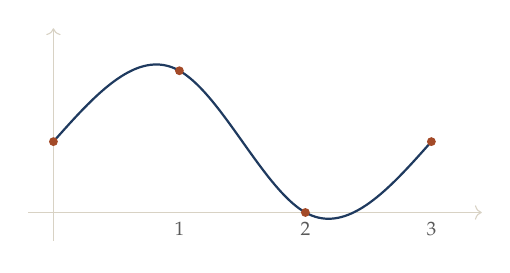
\begin{tikzpicture}[x=1.6cm,y=0.9cm]
\draw[->,linie] (-0.2,0)--(3.4,0); \draw[->,linie] (0,-0.4)--(0,2.6);
\draw[tief,thick,domain=0:1,samples=40,smooth] plot (\x,{1+2*\x-\x*\x*\x});
\draw[tief,thick,domain=1:2,samples=40,smooth] plot (\x,{2-(\x-1)-3*(\x-1)^2+2*(\x-1)^3});
\draw[tief,thick,domain=2:3,samples=40,smooth] plot (\x,{-(\x-2)+3*(\x-2)^2-(\x-2)^3});
\foreach \p in {(0,1),(1,2),(2,0),(3,1)} \fill[akzent] \p circle (1.6pt);
\foreach \x in {1,2,3} \node[below,font=\scriptsize,grau] at (\x,0) {\x};
\end{tikzpicture}
\end{center}
\probe{$S_1(2) = 2 - 1 - 3 + 2 = 0$, $S_2(3) = -1 + 3 - 1 = 1$. \checkmark\ Natürlich: $S_0''(0) = 0$, $S_2''(3) = 6 - 6 = 0$. \checkmark}
\begin{mitnehmen}\kastentext
Ein kubischer Spline ist zweimal stetig differenzierbar und minimiert $\int S''^{2}$ --- die Biegeenergie eines Lineals. Die Momentengleichungen sind tridiagonal und diagonaldominant: $O(n)$ Aufwand, keine Pivotisierung, kein Runge-Phänomen.
\end{mitnehmen}
\end{loesungkarte}

%%%%%%%%%% 5.32
\stupserzwei{gruen}{$c_1 = \frac14(1 + 2i^{-1} + 1\cdot i^{-2} + 0) = \frac14(1 - 2i - 1) = -\frac i2$.}{22pt}
\begin{loesungkarte}{gruen}{5.32}{Eine DFT von Hand}
\derweg{$\omega = i$, Potenzen tabellieren, vier Summen.}
\schritt{Vorbereitung}
$N = 4$, $\omega = e^{2\pi i/4} = i$, $c_k = \frac14\sum_{j=0}^{3}y_j\,i^{-kj}$. Potenzen: $i^{0} = 1$, $i^{-1} = -i$, $i^{-2} = -1$, $i^{-3} = i$.
\schritt{Koeffizienten}
$c_0 = \frac14(1 + 2 + 1 + 0) = 1$. \\
$c_1 = \frac14(1 + 2(-i) + 1(-1) + 0) = \frac14(-2i) = -\frac i2$. \\
$c_2 = \frac14(1 + 2(-1) + 1(1) + 0) = 0$. \\
$c_3 = \frac14(1 + 2(i) + 1(-1) + 0) = \frac i2$.
\schritt{Deutung}
$c_0 = 1$: Mittelwert. $c_1 = -\frac i2$ und $c_3 = \overline{c_1}$: eine Schwingung der Grundfrequenz mit Amplitude $2|c_1| = 1$ und Phase $-\frac\pi2$, also ein Sinus. $c_2 = 0$: keine Nyquist-Komponente. Tatsächlich $y_j = 1 + \sin\frac{2\pi j}4$: $1, 2, 1, 0$. \checkmark
\probe{Parseval: $\frac14\sum|y_j|^{2} = \frac{1 + 4 + 1}4 = 1{,}5$; $\sum|c_k|^{2} = 1 + \frac14 + 0 + \frac14 = 1{,}5$. \checkmark}
\begin{mitnehmen}\kastentext
Für reelle Daten ist $c_{N-k} = \overline{c_k}$; die Hälfte der Koeffizienten ist redundant. Die FFT berechnet alle $N$ Koeffizienten in $O(N\log N)$ statt $O(N^{2})$ --- bei $N = 10^{6}$ der Unterschied zwischen Millisekunden und Stunden, und der Grund, warum digitale Signalverarbeitung existiert.
\end{mitnehmen}
\end{loesungkarte}

%%%%%%%%%% 5.33
\stupserzwei{gruen}{$c_0 = \frac{e - e^{-1}}2 = \sinh1 = 1{,}1752$, $c_1 = \frac32\cdot\frac2e = \frac3e = 1{,}1036$.}{22pt}
\begin{loesungkarte}{gruen}{5.33}{Beste Quadratmittel-Approximation}
\derweg{Projektion auf $P_0 = 1$, $P_1 = x$ mit $c_k = \frac{\langle f, P_k\rangle}{\langle P_k, P_k\rangle}$; dann Vergleich mit Taylor an den Rändern und in der Norm.}
\schritt{Koeffizienten}
$\langle1, 1\rangle = 2$, $\langle x, x\rangle = \frac23$, $\langle1, x\rangle = 0$ (orthogonal). $\langle e^{x}, 1\rangle = e - e^{-1} = 2{,}3504$, $c_0 = 1{,}1752$. $\langle e^{x}, x\rangle = [xe^{x} - e^{x}]_{-1}^{1} = 0 + 2e^{-1} = 0{,}7358$, $c_1 = \frac{0{,}7358}{2/3} = 1{,}1036$.
\schritt{Ergebnis}
$p(x) = 1{,}1752 + 1{,}1036x$. Taylor: $1 + x$.
\schritt{Vergleich}
Bei $x = 1$: $e = 2{,}718$; $p = 2{,}279$; Taylor $2$. Bei $x = -1$: $0{,}368$; $p = 0{,}072$; Taylor $0$. Bei $0$: $1$; $p = 1{,}175$; Taylor $1$ (exakt). Taylor ist in der Mitte besser und am Rand schlechter. In der $L^{2}$-Norm: $\|e^{x} - p\|_2 = 0{,}229$, $\|e^{x} - (1 + x)\|_2 = 0{,}348$. Die Projektion gewinnt --- sie ist dafür gebaut.
\probe{$\|e^{x}\|_2^{2} = \frac{e^{2} - e^{-2}}2 = 3{,}627$; $\|p\|_2^{2} = 2c_0^{2} + \frac23c_1^{2} = 2{,}762 + 0{,}812 = 3{,}574$; Fehler$^{2}$ $= 0{,}053$, Fehler $0{,}230$ (Pythagoras). \checkmark}
\begin{mitnehmen}\kastentext
Orthogonale Polynome machen die Normalengleichungen diagonal: Jeder Koeffizient ist ein einzelnes Integral, und mehr Terme ändern die alten nicht. Taylor ist lokal optimal (bei $0$), die Projektion global --- für ein ganzes Intervall ist sie fast immer die bessere Wahl.
\end{mitnehmen}
\end{loesungkarte}

%%%%%%%%%% 5.34
\stupserzwei{gruen}{$r(0) = -b = E$, $r(1) = 1 - a - b = E$, $r(\frac a2) = -\frac{a^{2}}4 - b = -E$. Aus den ersten beiden: $a = 1$; dann $-\frac14 - b = b$, $b = -\frac18$.}{22pt}
\begin{loesungkarte}{gruen}{5.34}{Beste gleichmäßige Approximation}
\derweg{Drei Alternanten (Ränder und Scheitel), Alternanzbedingungen, lösen.}
\schritt{Ansatz}
$p(x) = ax + b$, $r(x) = x^{2} - ax - b$, nach oben geöffnete Parabel. Für $n = 1$ braucht man $n + 2 = 3$ Alternanten: die Ränder $0$, $1$ (Maxima von $r$) und den Scheitel $x = \frac a2$ (Minimum).
\schritt{Gleichungen}
$r(0) = -b = E$, $r(1) = 1 - a - b = E$, $r(\frac a2) = \frac{a^{2}}4 - \frac{a^{2}}2 - b = -\frac{a^{2}}4 - b = -E$.
\schritt{Lösen}
Aus den ersten beiden: $1 - a = 0$, $a = 1$. Dann $-\frac14 - b = -E = b$, also $b = -\frac18$, $E = \frac18$.
\schritt{Ergebnis}
$p(x) = x - \frac18$, Fehler $\|x^{2} - p\|_\infty = \frac18$, angenommen bei $0$ ($+$), $\frac12$ ($-$), $1$ ($+$).
\probe{$r(0) = \frac18$, $r(\frac12) = \frac14 - \frac12 + \frac18 = -\frac18$, $r(1) = 1 - 1 + \frac18 = \frac18$. \checkmark\ Zum Vergleich: die Sekante $p = x$ hat Fehler $\frac14$, die Tangente bei $\frac12$, $p = x - \frac14$, ebenfalls $\frac14$. Die Minimax-Lösung liegt genau dazwischen. \checkmark}
\begin{mitnehmen}\kastentext
Alternantensatz: $p_n$ ist die beste gleichmäßige Approximation genau dann, wenn der Fehler an $n + 2$ Stellen abwechselnd $\pm E$ annimmt. Für $x^{2}$ auf $[0, 1]$ ist der Fehler $\frac18 = \frac12\cdot2^{-2}$ --- das Tschebyschow-Polynom $T_2$, auf $[0, 1]$ transformiert. Der Remez-Algorithmus findet die Alternanten iterativ; Bibliotheken berechnen so $\sin$, $\exp$ und Co.
\end{mitnehmen}
\end{loesungkarte}

%%%%%%%%%% 5.35
\stupserzwei{tief}{Trapez-Fehler $1{,}55\cdot10^{-2}$; $3{,}84\cdot10^{-3}$; $9{,}59\cdot10^{-4}$; $2{,}40\cdot10^{-4}$: Quotienten $4{,}02$; $4{,}01$; $4{,}00$.}{22pt}
\begin{loesungkarte}{tief}{5.35}{Die Fehlerordnung messen}
\derweg{Fehler tabellieren, Quotienten bilden, $p = \log_2(\text{Quotient})$; Richardson aus zwei Werten.}
\schritt{(a)}
\begin{center}\footnotesize\setlength{\tabcolsep}{4pt}
\begin{tabular}{l|cccc}
$m$ & 2 & 4 & 8 & 16\\ \hline
Trapez-Fehler & $-1{,}55\cdot10^{-2}$ & $-3{,}84\cdot10^{-3}$ & $-9{,}59\cdot10^{-4}$ & $-2{,}40\cdot10^{-4}$\\
Quotient & & $4{,}02$ & $4{,}01$ & $4{,}00$\\ \hline
Simpson-Fehler & $3{,}56\cdot10^{-4}$ & $3{,}12\cdot10^{-5}$ & $1{,}99\cdot10^{-6}$ & $1{,}25\cdot10^{-7}$\\
Quotient & & $11{,}4$ & $15{,}7$ & $16{,}0$
\end{tabular}
\end{center}
Trapez: Quotient $4 = 2^{2}$, Ordnung $2$. Simpson: Quotient $\to16 = 2^{4}$, Ordnung $4$.
\schritt{(b)}
Fehler $\approx Ch^{2}$: $T(h) - I\approx4(T(h/2) - I)$, also $I\approx T(h/2) + \frac{T(h/2) - T(h)}3$. Mit $m = 4, 8$: $0{,}7458656 + \frac{0{,}0028815}3 = 0{,}7468261$ --- das ist Simpson mit $m = 8$, Fehler $2\cdot10^{-6}$. Die Fehlerschätzung $\frac{T(h/2) - T(h)}3 = 9{,}6\cdot10^{-4}$ trifft den wahren Fehler $9{,}59\cdot10^{-4}$ von $T(h/2)$.
\schritt{(c)}
Trapez: Fehler $\approx\frac{0{,}0615}{m^{2}}$; $10^{-10}$ bei $m\approx25\,000$. Simpson: Fehler $\approx\frac{0{,}0082}{m^{4}}$; $10^{-10}$ bei $m\approx96$. Faktor $260$ in den Funktionsauswertungen --- das ist der Wert einer höheren Ordnung.
\schritt{(d)}
Der Fehler ist $C_4h^{4} + C_6h^{6} + \dots$; bei grobem $h$ ist der $h^{6}$-Term noch spürbar, und der Quotient weicht von $16$ ab. Die Ordnung ist eine asymptotische Aussage: $p$ erkennt man erst, wenn $h$ klein genug ist. Umgekehrt: Bleibt der Quotient weit unter dem Erwarteten, fehlt der Funktion Glattheit --- oder dem Programm ein Faktor.
\probe{Trapezfehler-Vorzeichen: $-\frac{h^{2}}{12}\int f''$, und $\int_0^1f'' = f'(1) - f'(0) = -2e^{-1} < 0$: Fehler negativ (Trapez zu klein, Integrand konkav in der Mitte --- nein: $f'' < 0$ auf $[0, 0{,}7]$, Trapezsehnen liegen unter der Kurve). \checkmark}
\begin{mitnehmen}\kastentext
Ordnung messen: $p = \log_2\frac{e(h)}{e(h/2)}$. Das ist der wichtigste Test für jede Implementierung --- stimmt die Ordnung nicht, ist etwas falsch. Und Richardson: Aus zwei Näherungen der Ordnung $p$ wird eine der Ordnung $p + 2$ (bei geraden Entwicklungen), gratis.
\end{mitnehmen}
\end{loesungkarte}

%%%%%%%%%% 5.36
\stupserzwei{gruen}{Trapez $0{,}742984$, Simpson $0{,}746855$; exakt $0{,}746824$. Fehlerschranken: $\frac{h^{2}}{12}\max|f''| = 0{,}0104$, $\frac{h^{4}}{180}\max|f^{(4)}| = 2{,}6\cdot10^{-4}$.}{22pt}
\begin{loesungkarte}{gruen}{5.36}{Trapez und Simpson}
\derweg{Fünf Funktionswerte, zwei gewichtete Summen, Fehlerformeln mit Ableitungsschranken.}
\schritt{Funktionswerte}
$h = 0{,}25$: $f_0 = 1$, $f_1 = 0{,}939413$, $f_2 = 0{,}778801$, $f_3 = 0{,}569783$, $f_4 = 0{,}367879$.
\schritt{Trapez}
$T = h\bigl(\frac{f_0 + f_4}2 + f_1 + f_2 + f_3\bigr) = 0{,}25\cdot(0{,}683940 + 2{,}287997) = 0{,}742984$.
\schritt{Simpson}
$S = \frac h3(f_0 + 4f_1 + 2f_2 + 4f_3 + f_4) = \frac{0{,}25}3\cdot(1 + 3{,}757652 + 1{,}557602 + 2{,}279131 + 0{,}367879) = \frac{0{,}25}3\cdot8{,}962264 = 0{,}746855$.
\schritt{Fehlerschranken}
$f'' = (4x^{2} - 2)e^{-x^{2}}$, $|f''|\le2$ auf $[0, 1]$ (bei $0$). Trapez: $|E|\le\frac{(b - a)h^{2}}{12}\max|f''| = \frac{0{,}0625}{12}\cdot2 = 0{,}0104$. Tatsächlich $0{,}0038$. \\
$f^{(4)} = (16x^{4} - 48x^{2} + 12)e^{-x^{2}}$, $|f^{(4)}|\le12$ (bei $0$). Simpson: $|E|\le\frac{(b - a)h^{4}}{180}\cdot12 = \frac{0{,}00390625\cdot12}{180} = 2{,}6\cdot10^{-4}$. Tatsächlich $3{,}1\cdot10^{-5}$.
\probe{$\int_0^1e^{-x^{2}}\,dx = \frac{\sqrt\pi}2\operatorname{erf}(1) = 0{,}886227\cdot0{,}842701 = 0{,}746824$. \checkmark\ Beide Schranken halten, mit Faktor $3$ bzw.\ $8$ Luft.}
\begin{mitnehmen}\kastentext
Simpson mit $5$ Punkten schlägt Trapez mit $5$ Punkten um zwei Größenordnungen --- Ordnung $4$ gegen $2$. Die Fehlerformeln brauchen Ableitungen, die man selten hat; in der Praxis ersetzt man sie durch den Vergleich zweier Schrittweiten (Aufgabe 5.35) oder durch Romberg (Aufgabe 5.37).
\end{mitnehmen}
\end{loesungkarte}

%%%%%%%%%% 5.37
\stupserzwei{gruen}{Trapezwerte $0{,}683940$; $0{,}731370$; $0{,}742984$; $0{,}745866$. Jede Spalte rechts entsteht aus zwei Nachbarn links.}{22pt}
\begin{loesungkarte}{gruen}{5.37}{Das Romberg-Schema}
\derweg{Trapezwerte mit $h, \frac h2, \frac h4, \frac h8$ (Rekursion nutzt alte Punkte), dann Richardson spaltenweise.}
\schritt{Erste Spalte}
$R_{0,0} = \frac12(1 + 0{,}367879) = 0{,}683940$. $R_{1,0} = \frac12R_{0,0} + 0{,}5\cdot f(0{,}5) = 0{,}341970 + 0{,}389400 = 0{,}731370$. $R_{2,0} = \frac12R_{1,0} + 0{,}25(f_1 + f_3) = 0{,}365685 + 0{,}377299 = 0{,}742984$. $R_{3,0} = \frac12R_{2,0} + 0{,}125\sum_{\text{neu}}f = 0{,}371492 + 0{,}374374 = 0{,}745866$.
\schritt{Schema}
$R_{k,j} = R_{k,j-1} + \frac{R_{k,j-1} - R_{k-1,j-1}}{4^{j} - 1}$:
\begin{center}\small
\begin{tabular}{c|llll}
$k$ & $j = 0$ & $j = 1$ & $j = 2$ & $j = 3$\\ \hline
0 & $0{,}6839397$ & & & \\
1 & $0{,}7313703$ & $0{,}7471804$ & & \\
2 & $0{,}7429841$ & $0{,}7468554$ & $0{,}7468337$ & \\
3 & $0{,}7458656$ & $0{,}7468261$ & $0{,}7468242$ & $0{,}7468240$
\end{tabular}
\end{center}
\schritt{Fehler}
Exakt $0{,}7468241$. Spalte $0$ (Trapez): $6\cdot10^{-2}$, $1{,}5\cdot10^{-2}$, $3{,}8\cdot10^{-3}$, $9{,}6\cdot10^{-4}$. Spalte $1$ (Simpson): $3{,}6\cdot10^{-4}$, $3{,}1\cdot10^{-5}$, $2{,}0\cdot10^{-6}$. Spalte $2$: $9{,}6\cdot10^{-6}$, $3{,}7\cdot10^{-8}$. Spalte $3$: $1{,}1\cdot10^{-7}$. \\
$R_{3,3}$ ist nicht besser als $R_{3,2}$: Die dritte Extrapolation setzt voraus, dass der $h^{6}$-Term schon dominiert, und $R_{2,2}$ war dafür zu grob. Bester Wert im Schema: $R_{3,2}$ mit $8$ richtigen Stellen --- aus $9$ Funktionswerten.
\probe{Spalte $1$ ist Simpson: $R_{2,1} = 0{,}7468554$ stimmt mit Aufgabe 5.36 überein. \checkmark\ Spalte $2$ ist die Boole-Regel (Ordnung $6$). \checkmark}
\begin{mitnehmen}\kastentext
Romberg ist Richardson-Extrapolation in Tabellenform: Jede Spalte gewinnt zwei Ordnungen. Voraussetzung ist die Euler--Maclaurin-Entwicklung des Trapezfehlers in geraden Potenzen von $h$ --- die gilt für glatte Integranden; bei Singularitäten oder Knicken bricht das Schema zusammen (Aufgabe 5.44).
\end{mitnehmen}
\end{loesungkarte}

%%%%%%%%%% 5.38
\stupserzwei{gruen}{Knoten $x = \frac{1\pm\sqrt{3/5}}2$ und $\frac12$: $0{,}1127$; $0{,}5$; $0{,}8873$. Gewichte $\frac5{18}, \frac8{18}, \frac5{18}$ (nach Transformation).}{22pt}
\begin{loesungkarte}{gruen}{5.38}{Gauß--Legendre mit drei Punkten}
\derweg{Transformieren, drei Funktionswerte, gewichtete Summe; Vergleich mit Simpson $m = 2$.}
\schritt{Transformation}
$x = \frac{t + 1}2$, $dx = \frac{dt}2$: $I = \frac12\int_{-1}^{1}e^{-((t + 1)/2)^{2}}\,dt$. Knoten $t = -\sqrt{3/5}, 0, \sqrt{3/5}$ mit Gewichten $\frac59, \frac89, \frac59$.
\schritt{Auswertung}
$x_0 = 0{,}112702$: $f = 0{,}987377$. $x_1 = 0{,}5$: $f = 0{,}778801$. $x_2 = 0{,}887298$: $f = 0{,}455062$. \\
$I\approx\frac12\bigl(\frac59\cdot0{,}987377 + \frac89\cdot0{,}778801 + \frac59\cdot0{,}455062\bigr) = \frac12\cdot(0{,}548543 + 0{,}692268 + 0{,}252812) = 0{,}746811$. Fehler $1{,}3\cdot10^{-5}$. (Mit mehr Stellen in den Funktionswerten: $0{,}7468146$, Fehler $9{,}5\cdot10^{-6}$.)
\schritt{Simpson mit drei Punkten}
$\frac16(f(0) + 4f(0{,}5) + f(1)) = \frac16(1 + 3{,}115203 + 0{,}367879) = 0{,}747180$. Fehler $3{,}6\cdot10^{-4}$.
\schritt{Vergleich}
Gleiche Punktzahl, Faktor $37$ im Fehler. Gauß ist exakt für Polynome bis Grad $5$, Simpson bis Grad $3$; die Fehlerterme sind $\sim f^{(6)}$ bzw.\ $\sim f^{(4)}$.
\probe{Exaktheit bis Grad $5$: $\int_{-1}^{1}t^{4}\,dt = \frac25$; Gauß: $2\cdot\frac59\cdot\frac9{25} = \frac25$. \checkmark\ Grad $6$: $\int t^{6} = \frac27$; Gauß: $2\cdot\frac59\cdot\frac{27}{125} = \frac6{25}\neq\frac27$ --- wie erwartet nicht mehr exakt.}
\begin{mitnehmen}\kastentext
$n$ Gauß-Punkte integrieren Polynome bis Grad $2n - 1$ exakt --- doppelt so viel wie jede Formel mit festen Knoten. Die Knoten sind die Nullstellen der Legendre-Polynome, die Gewichte positiv (keine Auslöschung). Für glatte Integranden ist Gauß das Verfahren der Wahl; für Daten auf festem Gitter bleibt Simpson.
\end{mitnehmen}
\end{loesungkarte}

%%%%%%%%%% 5.39
\stupserzwei{akzent}{Implizit: $y_{k+1} = y_k - 50hy_{k+1}$, also $y_{k+1} = \frac{y_k}{1 + 50h} = \frac{y_k}6$. Faktor $\frac16$ für jedes $h > 0$ kleiner als $1$.}{22pt}
\begin{loesungkarte}{akzent}{5.39}{Euler explodiert}
\derweg{Verstärkungsfaktor pro Schritt ausrechnen; Stabilität heißt $|\text{Faktor}| < 1$.}
\schritt{(a)}
$y_{k+1} = y_k + h(-50y_k) = (1 - 5)y_k = -4y_k$: $y_1 = -4$, $y_2 = 16$, $y_3 = -64$, $y_4 = 256$. Exakt: $y(0{,}1) = e^{-5} = 0{,}0067$, $y(0{,}4) = e^{-20} = 2\cdot10^{-9}$. Das Verfahren liefert exponentielles Wachstum mit Vorzeichenwechsel für eine Lösung, die praktisch sofort null ist.
\schritt{(b)}
Faktor $|1 - 50h| < 1\iff0 < h < \frac2{50} = 0{,}04$. Für $[0, 1]$ also mindestens $26$ Schritte --- obwohl die Lösung nach $t = 0{,}1$ nichts mehr tut. Die Schrittweite wird von der Stabilität diktiert, nicht von der Genauigkeit: Das ist Steifigkeit.
\schritt{(c)}
$y_{k+1} = \frac{y_k}{1 + 50h} = \frac{y_k}6$: $0{,}1667$; $0{,}0278$; $0{,}0046$; $0{,}0008$. Nicht genau (exakt $0{,}0067$ nach einem Schritt), aber qualitativ richtig: monoton fallend gegen $0$.
\schritt{(d)}
Faktor $\frac1{1 + 50h}$ liegt für jedes $h > 0$ in $(0, 1)$: A-stabil, keine Schrittweitenbeschränkung. Mit $h = 1$: $y_1 = \frac1{51}$ --- grob, aber stabil. Preis: Pro Schritt ist eine Gleichung nach $y_{k+1}$ zu lösen; bei nichtlinearem $f$ ein Newton-Verfahren (Aufgabe 5.26) in jedem Schritt.
\begin{center}
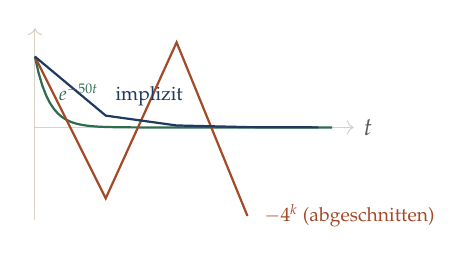
\begin{tikzpicture}[x=9cm,y=0.9cm]
\draw[->,linie] (0,0)--(0.45,0) node[right,grau,font=\small] {$t$}; \draw[->,linie] (0,-1.3)--(0,1.4);
\draw[gruen,thick,domain=0:0.42,samples=80] plot (\x,{exp(-50*\x)});
\draw[akzent,thick] (0,1)--(0.1,-1)--(0.2,1.2)--(0.3,-1.25); \node[akzent,font=\scriptsize,right] at (0.31,-1.25) {$-4^{k}$ (abgeschnitten)};
\draw[tief,thick] (0,1)--(0.1,0.1667)--(0.2,0.0278)--(0.3,0.0046)--(0.4,0.0008);
\node[gruen,font=\scriptsize,right] at (0.02,0.5) {$e^{-50t}$}; \node[tief,font=\scriptsize,above right] at (0.1,0.17) {implizit};
\end{tikzpicture}
\end{center}
\begin{fehler}\kastentext
\enquote{Kleinere Schrittweite, kleinerer Fehler} gilt nur innerhalb des Stabilitätsgebiets. Außerhalb explodiert das Verfahren, egal wie glatt die Lösung ist. Steife Probleme (chemische Kinetik, Schaltkreise, parabolische PDE nach Ortsdiskretisierung) erkennt man daran, dass explizite Verfahren absurd kleine Schritte verlangen.
\end{fehler}
\begin{mitnehmen}\kastentext
Testgleichung $y' = \lambda y$: Explizites Euler ist stabil für $|1 + h\lambda| < 1$, implizites für alle $\operatorname{Re}\lambda < 0$. Bei steifen Systemen ist $|\lambda|$ groß (schnell abklingende Komponenten), und nur implizite Verfahren (oder spezielle wie BDF, Band 29) kommen mit vernünftigen Schrittweiten aus.
\end{mitnehmen}
\end{loesungkarte}

%%%%%%%%%% 5.40
\stupserzwei{gruen}{RK4 erster Schritt: $k_1 = 1{,}5$, $k_2 = 1{,}64$, $k_3 = 1{,}654$, $k_4 = 1{,}7908$; $y_1 = 0{,}5 + \frac{0{,}2}6(k_1 + 2k_2 + 2k_3 + k_4) = 0{,}829293$.}{22pt}
\begin{loesungkarte}{gruen}{5.40}{Euler und Runge--Kutta}
\derweg{Euler: eine Steigung. RK4: vier Steigungen pro Schritt, gewichtet.}
\schritt{Exakt}
$y(0{,}2) = 1{,}44 - 0{,}5e^{0{,}2} = 0{,}829299$, $y(0{,}4) = 1{,}96 - 0{,}5e^{0{,}4} = 1{,}214088$.
\schritt{Euler}
$f(t, y) = y - t^{2} + 1$. $y_1 = 0{,}5 + 0{,}2\cdot(0{,}5 + 1) = 0{,}8$. $y_2 = 0{,}8 + 0{,}2\cdot(0{,}8 - 0{,}04 + 1) = 1{,}152$. Fehler $0{,}029$ und $0{,}062$.
\schritt{RK4, Schritt 1}
$k_1 = f(0;\ 0{,}5) = 1{,}5$. $k_2 = f(0{,}1;\ 0{,}65) = 0{,}65 - 0{,}01 + 1 = 1{,}64$. $k_3 = f(0{,}1;\ 0{,}664) = 1{,}654$. $k_4 = f(0{,}2;\ 0{,}8308) = 0{,}8308 - 0{,}04 + 1 = 1{,}7908$. $y_1 = 0{,}5 + \frac{0{,}2}6(1{,}5 + 3{,}28 + 3{,}308 + 1{,}7908) = 0{,}5 + 0{,}329293 = 0{,}829293$. Fehler $5\cdot10^{-6}$.
\schritt{RK4, Schritt 2}
$k_1 = f(0{,}2;\ 0{,}829293) = 1{,}789293$. $k_2 = f(0{,}3;\ 1{,}008222) = 1{,}918222$. $k_3 = f(0{,}3;\ 1{,}021115) = 1{,}931115$. $k_4 = f(0{,}4;\ 1{,}215516) = 2{,}055516$. $y_2 = 0{,}829293 + \frac{0{,}2}6(1{,}789293 + 3{,}836444 + 3{,}862230 + 2{,}055516) = 0{,}829293 + 0{,}384783 = 1{,}214076$. Fehler $1{,}1\cdot10^{-5}$.
\schritt{Vergleich}
Euler: Fehler in der zweiten Dezimale ($3\,\%$). RK4: in der fünften, bei viermal so vielen Funktionsauswertungen. Mit $h = 0{,}05$ hätte Euler Fehler $0{,}016$ (Ordnung $1$: Viertelung der Schrittweite viertelt den Fehler), RK4 bei gleichem Aufwand $4\cdot10^{-8}$ (Ordnung $4$: Faktor $256$).
\probe{Exakte Lösung einsetzen: $y' = 2(t + 1) - 0{,}5e^{t}$; $y - t^{2} + 1 = t^{2} + 2t + 1 - 0{,}5e^{t} - t^{2} + 1 = 2t + 2 - 0{,}5e^{t}$. \checkmark}
\begin{mitnehmen}\kastentext
RK4 ist das Arbeitspferd für nicht-steife Probleme: Ordnung $4$ für vier Auswertungen, einfach zu programmieren, keine Vergangenheit nötig. Moderne Löser (Dormand--Prince) nehmen zwei RK-Formeln verschiedener Ordnung gleichzeitig, schätzen daraus den Fehler und steuern $h$ --- Band 29.
\end{mitnehmen}
\end{loesungkarte}

%%%%%%%%%% 5.41
\stupserzwei{gruen}{$16\begin{pmatrix}2 & -1 & 0\\ -1 & 2 & -1\\ 0 & -1 & 2\end{pmatrix}u = \pi^{2}\begin{pmatrix}0{,}7071\\ 1\\ 0{,}7071\end{pmatrix}$; Symmetrie gibt $u_1 = u_3$.}{22pt}
\begin{loesungkarte}{gruen}{5.41}{Ein Randwertproblem auf drei Punkten}
\derweg{Zweite Ableitung durch den zentralen Differenzenquotienten, tridiagonales System, Symmetrie ausnutzen.}
\schritt{Diskretisierung}
$h = \frac14$, innere Punkte $0{,}25$, $0{,}5$, $0{,}75$. $-u''(x_i)\approx\frac{-u_{i-1} + 2u_i - u_{i+1}}{h^{2}}$, $u_0 = u_4 = 0$. System: $16(2u_1 - u_2) = f_1$, $16(-u_1 + 2u_2 - u_3) = f_2$, $16(-u_2 + 2u_3) = f_3$ mit $f_1 = f_3 = \pi^{2}\sin\frac\pi4 = 6{,}9792$, $f_2 = \pi^{2} = 9{,}8696$.
\schritt{Lösen}
Symmetrie: $u_1 = u_3$. Erste Gleichung: $u_2 = 2u_1 - \frac{6{,}9792}{16} = 2u_1 - 0{,}43620$. Zweite: $16(-2u_1 + 2u_2) = 9{,}8696$, also $u_2 - u_1 = 0{,}30843$. Einsetzen: $u_1 - 0{,}43620 = 0{,}30843$, $u_1 = 0{,}74463$, $u_2 = 1{,}05306$.
\schritt{Vergleich}
Exakt: $\sin\frac\pi4 = 0{,}70711$, $\sin\frac\pi2 = 1$. Fehler $0{,}0375$ und $0{,}0531$ --- etwa $5\,\%$. Theoretisch $\approx\frac{h^{2}}{12}\max|u^{(4)}| = \frac{0{,}0625}{12}\pi^{4}\cdot u = 0{,}507\cdot0{,}0625\cdot\dots$ --- genauer: Der Fehler ist $\frac{h^{2}\pi^{2}}{12}u(x) + O(h^{4}) = 0{,}0514\,u(x)$: $0{,}0364$ und $0{,}0514$. \checkmark
\probe{Mit $h = \frac18$ ($7$ innere Punkte) wäre der Fehler ein Viertel: $0{,}013$ in der Mitte. Ordnung $2$. \checkmark\ Die Matrix ist symmetrisch, positiv definit, diagonaldominant: Cholesky, Jacobi, CG --- alles geht.}
\begin{mitnehmen}\kastentext
Finite Differenzen: Ableitung durch Differenzenquotient, Differentialgleichung durch Gleichungssystem, Fehler $O(h^{2})$. In zwei Dimensionen wird aus der Tridiagonalmatrix der Fünf-Punkte-Stern mit $n^{2}$ Unbekannten --- und ab da sind iterative Löser (Kapitel 5) keine Option mehr, sondern Pflicht.
\end{mitnehmen}
\end{loesungkarte}

%%%%%%%%%% 5.42
\stupserzwei{tief}{Schritt 1: $g = (20, 20)$, $\alpha = \frac{800}{8800} = \frac1{11}$, neu $(8{,}18;\ -0{,}82)$, $f = 73{,}6$. Die Quotienten $\frac{73{,}6}{110} = \frac{49{,}3}{73{,}6} = 0{,}669 = \bigl(\frac9{11}\bigr)^{2}$.}{22pt}
\begin{loesungkarte}{tief}{5.42}{Gradientenverfahren im Tal}
\derweg{Gradient, exakte Schrittweite $\alpha = \frac{g^{\mathsf T}g}{g^{\mathsf T}Ag}$, Update; Quotienten mit der Theorie vergleichen; Newton zum Kontrast.}
\schritt{(a)}
$A = \operatorname{diag}(2, 20)$, $\nabla f = Ax$, $f(10, 1) = 110$.
\begin{center}\small
\begin{tabular}{c|ccc|c}
$k$ & $x$ & $\nabla f$ & $\alpha$ & $f$\\ \hline
0 & $(10;\ 1)$ & $(20;\ 20)$ & $0{,}0909$ & $110$\\
1 & $(8{,}18;\ -0{,}82)$ & $(16{,}4;\ -16{,}4)$ & $0{,}0909$ & $73{,}6$\\
2 & $(6{,}69;\ 0{,}67)$ & $(13{,}4;\ 13{,}4)$ & $0{,}0909$ & $49{,}3$\\
3 & $(5{,}48;\ -0{,}55)$ & & & $33{,}0$
\end{tabular}
\end{center}
Die Iterierten zickzacken: $y$ wechselt das Vorzeichen, $x$ schrumpft langsam.
\schritt{(b)}
Quotienten $\frac{73{,}6}{110} = 0{,}669$, $\frac{49{,}3}{73{,}6} = 0{,}669$, $\frac{33{,}0}{49{,}3} = 0{,}669$. Theorie: $\bigl(\frac{\kappa - 1}{\kappa + 1}\bigr)^{2} = \bigl(\frac9{11}\bigr)^{2} = 0{,}669$ --- hier exakt, weil der Start die schlechteste Richtung trifft.
\schritt{(c)}
Newton: $x_1 = x_0 - H^{-1}\nabla f = x_0 - A^{-1}Ax_0 = 0$. Ein Schritt, fertig --- bei quadratischem $f$ ist das Newton-Modell exakt.
\schritt{(d)}
$\kappa = 1000$: Faktor $\bigl(\frac{999}{1001}\bigr)^{2} = 0{,}996$ pro Schritt. Für $10^{-6}$: $\frac{\ln10^{-6}}{\ln0{,}996} = 3450$ Schritte. Das Gradientenverfahren ist für schlecht konditionierte Probleme unbrauchbar; CG braucht $\sim\sqrt\kappa = 32$ Schritte, Newton einen.
\probe{Exakte Liniensuche heißt: Der neue Gradient steht senkrecht auf dem alten. $(16{,}4;\ -16{,}4)\cdot(20;\ 20) = 0$. \checkmark}
\begin{mitnehmen}\kastentext
Steilster Abstieg: billig pro Schritt, aber Rate $\frac{\kappa - 1}{\kappa + 1}$ --- in langen Tälern hoffnungslos. Abhilfen: Vorkonditionierung (das Tal rund machen), konjugierte Richtungen (CG), Krümmungsinformation (Newton, Quasi-Newton). Rosenbrock (Aufgabe 5.43) ist der Testfall für alle drei.
\end{mitnehmen}
\end{loesungkarte}

%%%%%%%%%% 5.43
\stupserzwei{gruen}{$Hs = -\nabla F$: $\begin{pmatrix}802 & 400\\ 400 & 200\end{pmatrix}s = \begin{pmatrix}4\\ 0\end{pmatrix}$, $\det = 400$, $s = (2, -4)$. Neu: $(1, -3)$, $F = 1600$.}{22pt}
\begin{loesungkarte}{gruen}{5.43}{Ein Newton-Schritt auf Rosenbrock}
\derweg{Gradient und Hesse-Matrix am Startpunkt, lineares System, Schritt --- und dann $F$ vergleichen.}
\schritt{Ableitungen}
$F_x = -2(1 - x) - 400x(y - x^{2})$, $F_y = 200(y - x^{2})$. $F_{xx} = 2 - 400(y - x^{2}) + 800x^{2}$, $F_{xy} = -400x$, $F_{yy} = 200$.
\schritt{Bei $(-1, 1)$}
$y - x^{2} = 0$: $\nabla F = (-4, 0)$, $H = \begin{pmatrix}802 & 400\\ 400 & 200\end{pmatrix}$, $F = 4$.
\schritt{Newton-Schritt}
$Hs = -\nabla F = (4, 0)$. $\det H = 160\,400 - 160\,000 = 400$. $s = \frac1{400}\begin{pmatrix}200 & -400\\ -400 & 802\end{pmatrix}\begin{pmatrix}4\\ 0\end{pmatrix} = \frac1{400}(800, -1600) = (2, -4)$. Neuer Punkt $(1, -3)$.
\schritt{Bewertung}
$F(1, -3) = 0 + 100(-3 - 1)^{2} = 1600$ --- vierhundertmal schlechter als $F = 4$. Die $x$-Koordinate ist perfekt ($1$), die $y$-Koordinate liegt weit unter dem Tal ($y$ sollte $x^{2} = 1$ sein). Das quadratische Modell ist am Startpunkt gut, aber $2$ Einheiten weit entfernt nicht mehr --- $F$ ist quartisch.
\schritt{Dämpfung}
$x_0 + \alpha s$: $\alpha = 1$: $1600$; $\alpha = \frac12$: $(0, -1)$, $F = 101$; $\alpha = \frac14$: $(-0{,}5;\ 0)$, $F = 8{,}5$; $\alpha = 0{,}1$: $(-0{,}8;\ 0{,}6)$, $F = 3{,}4 < 4$. Erst die Schrittweite $0{,}1$ ist ein Abstieg. Gedämpftes Newton (Armijo) nimmt diesen Schritt --- und ist in etwa $20$ Schritten am Ziel; ungedämpft wird es ein Zickzack.
\probe{$H$ ist positiv definit ($802 > 0$, $\det > 0$): Die Newton-Richtung ist eine Abstiegsrichtung, $\nabla F\cdot s = -8 < 0$. \checkmark\ Das Problem ist nicht die Richtung, sondern die Länge.}
\begin{mitnehmen}\kastentext
Newton für Optimierung: Richtung aus dem quadratischen Modell, Länge aus einer Liniensuche. Ohne Liniensuche vertraut man dem Modell blind --- und auf Rosenbrocks gekrümmtem Tal kostet das. Trust-Region-Verfahren begrenzen den Schritt von vornherein; beides ist Band 19.
\end{mitnehmen}
\end{loesungkarte}

%%%%%%%%%% 5.44
\stupserzwei{gruen}{Standardabweichung von $\hat\pi$: $4\sqrt{\frac{p(1 - p)}N} = \frac{1{,}64}{\sqrt N}$. Für $\pm5\cdot10^{-4}$ als eine Standardabweichung: $N\approx1{,}1\cdot10^{7}$.}{22pt}
\begin{loesungkarte}{gruen}{5.44}{$\pi$ mit Monte-Carlo}
\derweg{Trefferanteil als Binomialschätzer; Standardabweichung; nach $N$ auflösen; dann Simpson zum Vergleich.}
\schritt{Verfahren}
$N$ Punkte gleichverteilt in $[0, 1]^{2}$; Anteil $\hat p$ mit $x^{2} + y^{2}\le1$ schätzt $\frac\pi4$; $\hat\pi = 4\hat p$.
\schritt{Genauigkeit}
Treffer sind $\operatorname{Bin}(N, p)$ mit $p = \frac\pi4 = 0{,}785$. $\operatorname{sd}(\hat p) = \sqrt{\frac{p(1 - p)}N} = \frac{0{,}411}{\sqrt N}$, $\operatorname{sd}(\hat\pi) = \frac{1{,}64}{\sqrt N}$. Drei sichere Nachkommastellen: Fehler $< 5\cdot10^{-4}$. Als eine Standardabweichung: $N = \bigl(\frac{1{,}64}{5\cdot10^{-4}}\bigr)^{2} = 1{,}1\cdot10^{7}$. Mit $95\,\%$ Sicherheit (zwei Standardabweichungen): $4{,}3\cdot10^{7}$ Punkte.
\schritt{Simpson}
$4\int_0^1\sqrt{1 - x^{2}}\,dx$: $m = 10$: Fehler $1{,}5\cdot10^{-2}$; $m = 100$: $4{,}6\cdot10^{-4}$; $m = 1000$: $1{,}5\cdot10^{-5}$. Nur Ordnung $1{,}5$ statt $4$ --- die Wurzel hat bei $x = 1$ eine senkrechte Tangente, und das zerstört die Fehlerentwicklung. Trotzdem: $100$ Auswertungen für drei Stellen, gegen $10^{7}$ Zufallspunkte.
\schritt{Einordnung}
Monte-Carlo: Fehler $\sim\frac1{\sqrt N}$, unabhängig von der Dimension und von der Glattheit. Für ein eindimensionales Integral absurd langsam; für ein $20$-dimensionales das einzige, was noch geht (Simpson bräuchte $100^{20}$ Punkte).
\probe{Mit $N = 10^{6}$ liefert eine Simulation typischerweise $\hat\pi\in[3{,}138;\ 3{,}145]$ --- zwei Stellen, Schwankung $\pm1{,}6\cdot10^{-3}$, wie die Formel sagt. \checkmark}
\begin{mitnehmen}\kastentext
$\frac1{\sqrt N}$ ist das Gesetz der großen Zahlen als Konvergenzrate (Aufgabe 4.31). Zehnmal mehr Genauigkeit kostet hundertmal mehr Punkte. Varianzreduktion (Importance Sampling, Quasi-Monte-Carlo) verbessert die Konstante oder den Exponenten --- Band 27.
\end{mitnehmen}
\end{loesungkarte}

\cleardoublepage
\setgebiet{7}{Geometrie}{mittel}
\chapter{Lösungen: Geometrie}

%%%%%%%%%% 6.1
\stupserzwei{tief}{(a) Die Dreiecke $SAP$ und $SBP$ haben $SA = SB$, $AP = BP$ und die gemeinsame Seite $SP$: SSS. Also sind die Winkel bei $S$ gleich.}{22pt}
\begin{loesungkarte}{tief}{6.1}{Winkelhalbierende und Lot}
\derweg{Konstruieren, dann zwei Dreiecke finden, die nach einem Kongruenzsatz gleich sind --- die gesuchte Gleichheit ist eine Folge davon.}
\schritt{(a) Konstruktion}
Kreis um $S$ mit beliebigem Radius schneidet die Schenkel in $A$ und $B$. Kreise um $A$ und $B$ mit gleichem Radius $> \frac12AB$ schneiden sich in $P$ (im Winkelfeld). Die Gerade $SP$ ist die Winkelhalbierende.
\schritt{(a) Beweis}
In den Dreiecken $SAP$ und $SBP$ gilt $SA = SB$ (gleicher Kreis um $S$), $AP = BP$ (gleiche Radien), $SP$ gemeinsam. Nach SSS sind sie kongruent, also $\angle ASP = \angle BSP$. $\blacksquare$
\schritt{(b) Konstruktion}
Kreis um $P$, der $g$ in $A$ und $B$ schneidet. Kreise um $A$ und $B$ mit gleichem Radius schneiden sich in $Q$ (auf der anderen Seite von $g$). $PQ$ ist das Lot.
\schritt{(b) Beweis}
$PQ$ ist die Mittelsenkrechte von $AB$ (Aufgabe 6.3): $P$ und $Q$ haben beide gleichen Abstand zu $A$ und $B$. Also steht $PQ$ senkrecht auf $AB = g$. $\blacksquare$
\schritt{(c)}
Halbieren braucht nur Kreise gleicher Radien --- eine quadratische Operation (Schnitt zweier Kreise). Dritteln des Winkels $60^{\circ}$ hieße $\cos20^{\circ}$ konstruieren, und das ist Nullstelle von $8x^{3} - 6x - 1$, eines irreduziblen kubischen Polynoms. Mit Zirkel und Lineal erreicht man nur Zahlen, deren Grad eine Zweierpotenz ist (Wantzel 1837, Band 11).
\probe{(a) Probe am rechten Winkel: $A = (1, 0)$, $B = (0, 1)$, $P = (1, 1)$ (Schnitt der Kreise mit Radius $1$); $SP$ ist die Diagonale $y = x$, Winkel $45^{\circ}$. \checkmark}
\begin{mitnehmen}\kastentext
Jede Konstruktion ist ein Satz: \enquote{Wenn man so zeichnet, dann gilt \dots} Der Beweis benennt die kongruenten Dreiecke und den Kongruenzsatz. Und fast immer ist es SSS, weil der Zirkel gleiche Längen liefert.
\end{mitnehmen}
\end{loesungkarte}

%%%%%%%%%% 6.2
\stupserzwei{akzent}{$\sin\alpha = \frac{a\sin\beta}b = \frac{5\cdot0{,}5}3 = 0{,}833$: $\alpha = 56{,}4^{\circ}$ oder $123{,}6^{\circ}$. Beide passen, weil $\alpha + \beta < 180^{\circ}$ in beiden Fällen.}{22pt}
\begin{loesungkarte}{akzent}{6.2}{SSW ist kein Kongruenzsatz}
\derweg{Konstruieren, mit dem Sinussatz beide Lösungen finden, die Eindeutigkeitsbedingung ablesen.}
\schritt{(a)}
Zeichne $a = BC = 5$. Trage in $B$ den Winkel $\beta = 30^{\circ}$ an. Kreis um $C$ mit Radius $b = 3$: Er schneidet den freien Schenkel zweimal, in $A_1$ und $A_2$ --- weil $b = 3$ größer als der Abstand von $C$ zum Schenkel ($5\sin30^{\circ} = 2{,}5$) und kleiner als $a = 5$ ist. Zwei Dreiecke mit denselben Daten.
\schritt{(b)}
Sinussatz: $\frac{\sin\alpha}a = \frac{\sin\beta}b$, $\sin\alpha = \frac{5\cdot0{,}5}3 = 0{,}8333$. $\alpha_1 = 56{,}4^{\circ}$, $\alpha_2 = 180^{\circ} - 56{,}4^{\circ} = 123{,}6^{\circ}$. Dann $\gamma_1 = 93{,}6^{\circ}$, $c_1 = \frac{b\sin\gamma_1}{\sin\beta} = 5{,}99$; $\gamma_2 = 26{,}4^{\circ}$, $c_2 = 2{,}67$.
\schritt{(c)}
SsW: Der gegebene Winkel liegt der \emph{größeren} Seite gegenüber. Dann ist $\alpha$ gegenüber der kleineren Seite spitz (der größere Winkel liegt der größeren Seite gegenüber), und die zweite Lösung $180^{\circ} - \alpha$ fällt weg. Hier läge $\beta$ gegenüber $b = 3 < a = 5$: nicht erfüllt. Mit $b = 6 > a$ wäre der Kreis groß genug, nur einmal zu schneiden.
\schritt{(d)}
\enquote{Also sind sie kongruent} --- der Schluss von SSW auf Kongruenz ist falsch; (a) ist das Gegenbeispiel. Richtig wäre er, wenn zusätzlich $b\ge a$ bekannt wäre.
\begin{fehler}\kastentext
Vier Kongruenzsätze: SSS, SWS, WSW (und WWS), SsW. Nicht SSW, nicht WWW (das ist Ähnlichkeit). Der Sinussatz liefert aus $\sin\alpha$ immer zwei Winkel; welcher gilt, entscheidet die Geometrie --- und manchmal beide.
\end{fehler}
\begin{mitnehmen}\kastentext
Bei jeder Dreiecksberechnung mit Sinussatz: Prüfen, ob $180^{\circ} - \alpha$ auch passt. Der Kosinussatz hat dieses Problem nicht --- $\cos$ ist auf $[0^{\circ}, 180^{\circ}]$ injektiv, deshalb liefert SWS über den Kosinussatz immer eindeutig.
\end{mitnehmen}
\end{loesungkarte}

%%%%%%%%%% 6.3
\stupserzwei{gruen}{$APB$ und $AQB$ sind kongruent (SSS), also $\angle PAB = \angle QAB$. Damit sind $APM$ und $AQM$ kongruent (SWS), also $\angle AMP = \angle AMQ$ --- Nebenwinkel, die gleich sind, sind rechte.}{22pt}
\begin{loesungkarte}{gruen}{6.3}{Die Mittelsenkrechte}
\derweg{Zweimal Kongruenz: erst zeigen, dass $PQ$ die Strecke $AB$ halbiert, dann dass die Winkel bei $M$ rechte sind.}
\schritt{Konstruktion}
Kreise um $A$ und $B$ mit gleichem Radius $r > \frac12AB$ schneiden sich in $P$ und $Q$. Gerade $PQ$, Schnitt mit $AB$ in $M$.
\schritt{$PQ$ halbiert $AB$}
Dreiecke $APQ$ und $BPQ$: $AP = BP = r$, $AQ = BQ = r$, $PQ$ gemeinsam: SSS, kongruent. Also $\angle APQ = \angle BPQ$. Nun $APM$ und $BPM$: $AP = BP$, $PM$ gemeinsam, eingeschlossene Winkel gleich: SWS, kongruent. Also $AM = BM$. $M$ ist der Mittelpunkt.
\schritt{$PQ$ steht senkrecht}
Aus derselben Kongruenz: $\angle AMP = \angle BMP$. Die beiden sind Nebenwinkel (sie ergänzen sich zu $180^{\circ}$) und gleich, also je $90^{\circ}$. $\blacksquare$
\schritt{Umkehrung}
Jeder Punkt der Mittelsenkrechten hat gleichen Abstand zu $A$ und $B$, und nur diese Punkte: Die Mittelsenkrechte ist der Ort aller Punkte mit $XA = XB$ --- der Grund, warum sich drei Mittelsenkrechten in einem Punkt treffen (Aufgabe 6.5).
\probe{Koordinaten: $A = (-1, 0)$, $B = (1, 0)$, $r = 2$: Kreise $(x\pm1)^{2} + y^{2} = 4$ schneiden sich bei $x = 0$, $y = \pm\sqrt3$. $PQ$ ist die $y$-Achse. \checkmark}
\begin{mitnehmen}\kastentext
Der Beweis braucht $r > \frac12AB$ (sonst schneiden sich die Kreise nicht) und die Tatsache, dass gleiche Nebenwinkel rechte sind. Das sind genau die Stellen, an denen Euklid in den \emph{Elementen} (I.10 und I.11) ebenfalls argumentiert.
\end{mitnehmen}
\end{loesungkarte}

%%%%%%%%%% 6.4
\stupserzwei{tief}{Die Höhe $12$ auf $b = 14$ teilt sie in $5$ und $9$: Die beiden Teildreiecke sind $5$-$12$-$13$ und $9$-$12$-$15$ --- beide pythagoreisch.}{22pt}
\begin{loesungkarte}{tief}{6.4}{Das 13-14-15-Dreieck}
\derweg{Heron, dann Höhe aus der Fläche, dann $r = A/s$, $R = abc/4A$, dann Kosinussatz als Probe.}
\schritt{(a)}
$s = \frac{13 + 14 + 15}2 = 21$. $A = \sqrt{21\cdot8\cdot7\cdot6} = \sqrt{7056} = 84$.
\schritt{(b)}
$h_b = \frac{2A}b = \frac{168}{14} = 12$. Der Fußpunkt teilt $b$: $\sqrt{13^{2} - 12^{2}} = 5$ und $\sqrt{15^{2} - 12^{2}} = 9$, $5 + 9 = 14$. \checkmark\ Das Dreieck ist aus einem $5$-$12$-$13$- und einem $9$-$12$-$15$-Dreieck zusammengesetzt --- deshalb die schönen Zahlen.
\schritt{(c)}
$r = \frac As = \frac{84}{21} = 4$. $R = \frac{abc}{4A} = \frac{2730}{336} = \frac{65}8 = 8{,}125$.
\schritt{(d)}
$\cos\alpha = \frac{b^{2} + c^{2} - a^{2}}{2bc} = \frac{196 + 225 - 169}{420} = \frac{252}{420} = 0{,}6$, $\alpha = 53{,}13^{\circ}$, $\sin\alpha = 0{,}8$. $A = \frac12\cdot14\cdot15\cdot0{,}8 = 84$. \checkmark
\probe{$\cos\beta = \frac{169 + 225 - 196}{390} = \frac{198}{390} = 0{,}5077$, $\beta = 59{,}5^{\circ}$; $\cos\gamma = \frac{169 + 196 - 225}{364} = \frac{140}{364} = 0{,}3846$, $\gamma = 67{,}4^{\circ}$. Summe $53{,}1 + 59{,}5 + 67{,}4 = 180{,}0$. \checkmark\ Euler: $R\ge2r$: $8{,}125\ge8$. \checkmark}
\begin{mitnehmen}\kastentext
Die Formeln, die man braucht: Heron $A = \sqrt{s(s - a)(s - b)(s - c)}$, $A = rs$, $A = \frac{abc}{4R}$, $A = \frac12bc\sin\alpha$. Vier Ausdrücke für dieselbe Fläche --- und jeder löst eine andere Aufgabe. Das $13$-$14$-$15$-Dreieck ist das kleinste mit ganzzahligen Seiten, Fläche, Höhe und Inkreisradius ohne rechten Winkel.
\end{mitnehmen}
\end{loesungkarte}

%%%%%%%%%% 6.5
\stupserzwei{gruen}{$U = (3, 1)$, $H = (2, 2)$, $S = (\frac83, \frac43)$. Prüfen: $S - U = (-\frac13, \frac13)$, $H - U = (-1, 1)$ --- parallel, Verhältnis $1 : 3$.}{22pt}
\begin{loesungkarte}{gruen}{6.5}{Die Eulergerade}
\derweg{Drei Punkte ausrechnen, dann prüfen, ob die Verbindungsvektoren parallel sind.}
\schritt{Schwerpunkt}
$S = \frac{A + B + C}3 = \bigl(\frac83, \frac43\bigr)$.
\schritt{Umkreismittelpunkt}
Mittelsenkrechte von $AB$: $x = 3$. Mittelsenkrechte von $AC$: Mittelpunkt $(1, 2)$, Richtung von $AC$ ist $(2, 4)$, also $2(x - 1) + 4(y - 2) = 0$, $x + 2y = 5$. Schnitt: $x = 3$, $y = 1$. $U = (3, 1)$. Probe: $UA = \sqrt{9 + 1} = \sqrt{10}$, $UB = \sqrt{9 + 1}$, $UC = \sqrt{1 + 9}$. \checkmark
\schritt{Höhenschnittpunkt}
Höhe von $C$ auf $AB$: $x = 2$. Höhe von $A$ auf $BC$: $BC = (-4, 4)$, also Richtung $(1, 1)$ durch $A$: $y = x$. Schnitt: $H = (2, 2)$. Probe: Höhe von $B$ auf $AC$: Richtung senkrecht zu $(2, 4)$, also $(2, -1)$: $(6, 0) + t(2, -1)$ trifft $(2, 2)$ bei $t = -2$. \checkmark
\schritt{Eulergerade}
$H - U = (-1, 1)$, $S - U = \bigl(-\frac13, \frac13\bigr) = \frac13(H - U)$. $S$ liegt auf $UH$ und teilt die Strecke im Verhältnis $US : SH = 1 : 2$. Genau Eulers Satz.
\probe{Allgemein gilt $H = A + B + C - 2U$ (bei $U$ als Ursprung: $H = A + B + C$): $(8, 4) - (6, 2) = (2, 2)$. \checkmark}
\begin{mitnehmen}\kastentext
Mit $U$ als Ursprung ist $H = A + B + C$ und $S = \frac{A + B + C}3 = \frac H3$ --- die Eulergerade ist dann eine Zeile. Die richtige Wahl des Koordinatenursprungs ersetzt oft eine Seite Rechnung.
\end{mitnehmen}
\end{loesungkarte}

%%%%%%%%%% 6.6
\stupserzwei{tief}{Tangente in $P$ auf Kreis um $M$: $(P - M)\cdot(X - M) = r^{2}$, hier $3(x - 3) + 4(y + 2) = 25$.}{22pt}
\begin{loesungkarte}{tief}{6.6}{Eine Kreisgleichung lesen}
\derweg{Quadratisch ergänzen; Tangente über den Radiusvektor; Schnitt durch Einsetzen; Existenz über das Vorzeichen des Radiusquadrats.}
\schritt{(a)}
$(x^{2} - 6x + 9) + (y^{2} + 4y + 4) = 12 + 9 + 4$: $(x - 3)^{2} + (y + 2)^{2} = 25$. $M = (3, -2)$, $r = 5$.
\schritt{(b)}
$(6 - 3)^{2} + (2 + 2)^{2} = 9 + 16 = 25$. \checkmark\ Tangente: senkrecht zum Radius $P - M = (3, 4)$ durch $P$: $3(x - 6) + 4(y - 2) = 0$, also $3x + 4y = 26$.
\schritt{(c)}
$y = x - 1$ einsetzen: $x^{2} + (x - 1)^{2} - 6x + 4(x - 1) - 12 = 2x^{2} - 4x - 15 = 0$, $x = \frac{4\pm\sqrt{16 + 120}}4 = 1\pm\frac{\sqrt{34}}2$: $x_{1,2} = 3{,}915$ und $-1{,}915$, $y = x - 1$: Schnittpunkte $(3{,}915;\ 2{,}915)$ und $(-1{,}915;\ -2{,}915)$.
\schritt{(d)}
$(x - 3)^{2} + (y + 2)^{2} = 13 - c$. Für $c > 13$ ist die rechte Seite negativ: keine Lösung. Für $c = 13$ nur der Punkt $M$, für $c < 13$ ein Kreis mit $r = \sqrt{13 - c}$.
\probe{(c) Abstand von $M$ zur Geraden $x - y - 1 = 0$: $\frac{|3 + 2 - 1|}{\sqrt2} = 2{,}83 < 5$: zwei Schnittpunkte. \checkmark\ Sehnenlänge $\sqrt2\cdot5{,}83 = 8{,}25$; und $2\sqrt{25 - 8} = 8{,}25$. \checkmark}
\begin{mitnehmen}\kastentext
Kreis: $|X - M| = r$. Tangente in $P$: $(P - M)\cdot(X - M) = r^{2}$. Lage einer Geraden: Abstand von $M$ mit $r$ vergleichen. Alles folgt aus dem Skalarprodukt --- und dasselbe gilt für die Kugel im Raum.
\end{mitnehmen}
\end{loesungkarte}

%%%%%%%%%% 6.7
\stupserzwei{gruen}{$PB = \frac{144}8 = 18$; die Tangentenlänge ist $\sqrt{144} = 12$ --- Pythagoras im Dreieck $P$, Mittelpunkt, Berührpunkt: $13^{2} = 5^{2} + 12^{2}$.}{22pt}
\begin{loesungkarte}{gruen}{6.7}{Die Potenz eines Punktes}
\derweg{Potenz ausrechnen; Sekantensatz und Tangentensatz sind dieselbe Gleichung.}
\schritt{Potenz}
$\operatorname{pot}(P) = d^{2} - r^{2} = 169 - 25 = 144$.
\schritt{Sekante}
$PA\cdot PB = \operatorname{pot}(P)$: $8\cdot PB = 144$, $PB = 18$. Die Sehne $AB$ hat Länge $10$ --- ein Durchmesser; die Sekante geht durch den Mittelpunkt (Probe: $PA = 13 - 5 = 8$). \checkmark
\schritt{Tangente}
$t^{2} = \operatorname{pot}(P) = 144$, $t = 12$. Pythagoras: Berührpunkt $T$, Dreieck $PTM$ rechtwinklig bei $T$: $PT^{2} = PM^{2} - r^{2} = 169 - 25$. \checkmark
\probe{Eine andere Sekante, etwa mit $PA' = 9$: $PB' = 16$, Sehne $7$. Das Produkt bleibt $144$, die Sehne variiert. \checkmark}
\begin{mitnehmen}\kastentext
Die Potenz ist eine Funktion des Punktes: negativ innen (Sehnensatz, $PA\cdot PB = r^{2} - d^{2}$), null auf dem Kreis, positiv außen (Sekanten-Tangenten-Satz). Der Ort der Punkte gleicher Potenz bezüglich zweier Kreise ist eine Gerade, die Potenzgerade --- der Schlüssel zu vielen Kreiskonstruktionen.
\end{mitnehmen}
\end{loesungkarte}

%%%%%%%%%% 6.8
\stupserzwei{gruen}{$PF_1 + PF_2 = 8{,}2 + 1{,}8 = 10 = 2a$. Tangente: $\frac{4x}{25} + \frac{1{,}8y}9 = 1$, also $4x + 5y = 25$.}{22pt}
\begin{loesungkarte}{gruen}{6.8}{Eine Ellipse vermessen}
\derweg{$c$ aus $a^{2} - b^{2}$; Abstände zu den Brennpunkten addieren; Tangentenformel.}
\schritt{(a)}
$c = \sqrt{25 - 9} = 4$, Brennpunkte $(\pm4, 0)$. $e = \frac ca = 0{,}8$. Leitlinien $x = \pm\frac ae = \pm\frac{a^{2}}c = \pm6{,}25$.
\schritt{(b)}
$P$ auf der Ellipse: $\frac{16}{25} + \frac{3{,}24}9 = 0{,}64 + 0{,}36 = 1$. \checkmark\ $PF_1 = \sqrt{(4 + 4)^{2} + 1{,}8^{2}} = \sqrt{67{,}24} = 8{,}2$, $PF_2 = \sqrt{0 + 3{,}24} = 1{,}8$. Summe $10 = 2a$. \checkmark\ Leitlinieneigenschaft: Abstand zu $F_2$ durch Abstand zur Leitlinie $x = 6{,}25$: $\frac{1{,}8}{2{,}25} = 0{,}8 = e$. \checkmark
\schritt{(c)}
Tangente in $(x_0, y_0)$: $\frac{x_0x}{a^{2}} + \frac{y_0y}{b^{2}} = 1$: $\frac{4x}{25} + \frac{1{,}8y}9 = 1$, mal $25$: $4x + 5y = 25$. Steigung $-\frac45$.
\probe{Mit Ableitung: $\frac{2x}{25} + \frac{2yy'}9 = 0$, $y' = -\frac{9x}{25y} = -\frac{36}{45} = -0{,}8$. \checkmark\ Die Tangente halbiert den Außenwinkel zwischen $PF_1$ und $PF_2$ (Reflexionseigenschaft): Richtungen $(-8, -1{,}8)$ und $(0, -1{,}8)$, Tangentenrichtung $(5, -4)$; Winkel zur Tangente: $\cos = \frac{-40 + 7{,}2}{8{,}2\cdot6{,}4} = -0{,}625$ und $\frac{7{,}2}{1{,}8\cdot6{,}4} = 0{,}625$ --- gleich groß. \checkmark}
\begin{mitnehmen}\kastentext
Drei Definitionen, eine Kurve: Summe der Brennpunktabstände $2a$ (Gärtner), Abstandsverhältnis $e < 1$ zur Leitlinie (Kegelschnitt), Gleichung $\frac{x^{2}}{a^{2}} + \frac{y^{2}}{b^{2}} = 1$ (analytisch). Dieselben drei gibt es für Parabel ($e = 1$) und Hyperbel ($e > 1$).
\end{mitnehmen}
\end{loesungkarte}

%%%%%%%%%% 6.9
\stupserzwei{tief}{$u\times v = (1, 1, 0)\times(0, 1, 2) = (2, -2, 1)$, $|u\times v| = 3$. Verbindungsvektor $(-1, 0, 1)$: Abstand $\frac{|-2 + 0 + 1|}3 = \frac13$.}{22pt}
\begin{loesungkarte}{tief}{6.9}{Windschief}
\derweg{Nicht parallel, Gleichsetzen führt zum Widerspruch; Abstand über das Kreuzprodukt; Lotpunkte über zwei Orthogonalitätsbedingungen.}
\schritt{(a)}
Richtungen $(1, 1, 0)$ und $(0, 1, 2)$ sind keine Vielfachen: nicht parallel. Gleichsetzen: $1 + s = 0$, $s = t$, $0 = 1 + 2t$ --- aus den ersten beiden $s = t = -1$, dann $0 = -1$. Kein Schnittpunkt. Windschief.
\schritt{(b)}
$n = u\times v = (2, -2, 1)$, $|n| = 3$. $d = \frac{|(Q - P)\cdot n|}{|n|} = \frac{|(-1, 0, 1)\cdot(2, -2, 1)|}3 = \frac13$.
\schritt{(c)}
$P(s) = (1 + s, s, 0)$, $Q(t) = (0, t, 1 + 2t)$, $Q - P = (-1 - s, t - s, 1 + 2t)$. Senkrecht zu $u$: $-1 - s + t - s = 0$. Senkrecht zu $v$: $t - s + 2 + 4t = 0$. Aus der ersten $t = 1 + 2s$, in die zweite: $5(1 + 2s) - s + 2 = 0$, $s = -\frac79$, $t = -\frac59$. Lotpunkte $P = \bigl(\frac29, -\frac79, 0\bigr)$, $Q = \bigl(0, -\frac59, -\frac19\bigr)$; $Q - P = \bigl(-\frac29, \frac29, -\frac19\bigr)$, Länge $\frac13$. \checkmark
\schritt{(d)}
Ebene durch $(1, 0, 0)$ mit Normale $n$: $2x - 2y + z = 2$. Sie enthält $g$ (Richtung $u\perp n$) und ist parallel zu $h$ ($v\perp n$); $h$ liegt im Abstand $\frac13$ darüber.
\probe{$Q - P$ ist parallel zu $n$: $\bigl(-\frac29, \frac29, -\frac19\bigr) = -\frac19(2, -2, 1)$. \checkmark}
\begin{mitnehmen}\kastentext
Zwei Geraden im Raum: Richtungen vergleichen (parallel?), Gleichsetzen (Schnitt?), sonst windschief. Der Abstand ist die Projektion des Verbindungsvektors auf die gemeinsame Normale $u\times v$ --- dieselbe Formel wie der Abstand Punkt--Ebene, denn $h$ liegt in einer zu $g$ parallelen Ebene.
\end{mitnehmen}
\end{loesungkarte}

%%%%%%%%%% 6.10
\stupserzwei{akzent}{(a) $54{,}7^{\circ}$ ist der Winkel zur \emph{Normalen}. Der Winkel zur Ebene ist $90^{\circ} - 54{,}7^{\circ} = 35{,}3^{\circ}$, und $\sin35{,}3^{\circ} = \frac1{\sqrt3}$.}{22pt}
\begin{loesungkarte}{akzent}{6.10}{Sinus oder Kosinus?}
\derweg{Jede Formel auf die Frage zurückführen: Winkel zwischen welchen zwei Vektoren? Richtung und Normale sind verschiedene Dinge.}
\schritt{(a)}
Das Skalarprodukt mit der Normalen gibt den Winkel zwischen Gerade und \emph{Normale}: $54{,}7^{\circ}$. Der Winkel zwischen Gerade und Ebene ist das Komplement: $35{,}3^{\circ}$. Formel: $\sin\varphi = \frac{|d\cdot n|}{|d||n|}$ --- Sinus, weil $\varphi = 90^{\circ} - \angle(d, n)$.
\schritt{(b)}
Winkel zwischen Ebenen $=$ Winkel zwischen Normalen: $\cos\varphi = \frac{|n_1\cdot n_2|}{|n_1||n_2|} = \frac{|(1, 1, 0)\cdot(0, 0, 1)|}{\sqrt2} = 0$, $\varphi = 90^{\circ}$. Zwei Ebenen bilden zwei Winkel ($\varphi$ und $180^{\circ} - \varphi$); gemeint ist der spitze --- daher der Betrag.
\schritt{(c)}
$\cos\varphi = \frac{(1, 0, 0)\cdot(1, 1, 0)}{1\cdot\sqrt2} = \frac1{\sqrt2}$, $\varphi = 45^{\circ}$. Mit $h'$: $\frac{-1}{\sqrt2}$, $135^{\circ}$ --- dieselbe Gerade, anderer Richtungsvektor. Der Winkel zwischen Geraden ist in $[0^{\circ}, 90^{\circ}]$: Betrag setzen, $45^{\circ}$.
\schritt{(d)}
\begin{center}\small
\begin{tabular}{l|l|l}
Objekte & Vektoren & Formel\\ \hline
Gerade--Gerade & Richtungen $d_1, d_2$ & $\cos\varphi = \frac{|d_1\cdot d_2|}{|d_1||d_2|}$\\
Ebene--Ebene & Normalen $n_1, n_2$ & $\cos\varphi = \frac{|n_1\cdot n_2|}{|n_1||n_2|}$\\
Gerade--Ebene & Richtung $d$, Normale $n$ & $\sin\varphi = \frac{|d\cdot n|}{|d||n|}$
\end{tabular}
\end{center}
\begin{fehler}\kastentext
Das Skalarprodukt misst den Winkel zwischen den \emph{Vektoren}, die man einsetzt. Bei Gerade und Ebene setzt man eine Richtung und eine Normale ein --- und bekommt das Komplement des gesuchten Winkels. Der Betrag im Zähler macht aus zwei möglichen Winkeln den spitzen.
\end{fehler}
\begin{mitnehmen}\kastentext
Vor jeder Winkelrechnung: Welche zwei Vektoren beschreiben die Objekte, und ist einer davon eine Normale? Eine Normale im Spiel: Vorzeichen des Komplements beachten. Zwei Normalen: Kosinus wie bei Geraden.
\end{mitnehmen}
\end{loesungkarte}

%%%%%%%%%% 6.11
\stupserzwei{gruen}{$12x + 7y + 11z = 59$; $D$ eingesetzt gibt $51$: Abstand $\frac8{\sqrt{314}} = 0{,}451$. Volumen $\frac86 = \frac43$.}{22pt}
\begin{loesungkarte}{gruen}{6.11}{Ebene, Abstand, Tetraeder}
\derweg{Normale aus dem Kreuzprodukt; Abstand als normierte Projektion; Volumen als Spatprodukt durch $6$; Winkel über das Skalarprodukt.}
\schritt{(a)}
$u = B - A = (3, -2, -2)$, $v = C - A = (1, 3, -3)$. $n = u\times v = \bigl((-2)(-3) - (-2)(3),\ (-2)(1) - (3)(-3),\ 3\cdot3 - (-2)(1)\bigr) = (12, 7, 11)$. Ebene: $12x + 7y + 11z = 12 + 14 + 33 = 59$. Probe mit $B$: $48 + 0 + 11 = 59$ \checkmark, $C$: $24 + 35 + 0 = 59$ \checkmark.
\schritt{(b)}
$D$ eingesetzt: $0 + 7 + 44 = 51$. $|n| = \sqrt{144 + 49 + 121} = \sqrt{314} = 17{,}72$. Abstand $\frac{|51 - 59|}{17{,}72} = 0{,}451$.
\schritt{(c)}
$V = \frac16|n\cdot(D - A)| = \frac16|(12, 7, 11)\cdot(-1, -1, 1)| = \frac16|-12 - 7 + 11| = \frac86 = \frac43$.
\schritt{(d)}
$\cos\varphi = \frac{u\cdot v}{|u||v|} = \frac{3 - 6 + 6}{\sqrt{17}\sqrt{19}} = \frac3{17{,}97} = 0{,}167$, $\varphi = 80{,}4^{\circ}$.
\probe{(c) anders: Grundfläche $\frac12|n| = 8{,}86$, Höhe $0{,}451$: $V = \frac13\cdot8{,}86\cdot0{,}451 = 1{,}33$. \checkmark}
\begin{mitnehmen}\kastentext
Kreuzprodukt: Normale und Flächeninhalt ($|u\times v|$ = Parallelogramm). Spatprodukt: Volumen ($|n\cdot w|$ = Spat, durch $6$ = Tetraeder). Skalarprodukt: Winkel und Abstände. Drei Produkte, und die ganze Raumgeometrie der Schule ist damit erledigt.
\end{mitnehmen}
\end{loesungkarte}

%%%%%%%%%% 6.12
\stupserzwei{akzent}{Die erweiterte $3\times3$-Matrix hat bei echten Kegelschnitten Determinante $\neq0$; bei (a), (c), (d), (e) ist sie $0$. (b) ist nicht entartet, nur leer.}{22pt}
\begin{loesungkarte}{akzent}{6.12}{Entartete Kegelschnitte}
\derweg{Faktorisieren, wo es geht; sonst Vorzeichen betrachten; die Determinante der erweiterten Matrix als Kriterium.}
\schritt{Die fünf Mengen}
(a) $(x - y)(x + y) = 0$: zwei sich schneidende Geraden $y = \pm x$. \\
(b) $x^{2} + y^{2} = -1$: leer (über $\mathbb R$). \\
(c) $(x - y)^{2} = 0$: eine Gerade $y = x$, doppelt gezählt. \\
(d) $(x - y)^{2} = 1$: zwei parallele Geraden $y = x\pm1$. \\
(e) $xy = 0$: die beiden Koordinatenachsen.
\schritt{Echt oder entartet}
Echte Kegelschnitte: Ellipse, Parabel, Hyperbel. (a), (c), (d), (e) sind Geradenpaare --- entartet. (b) ist keine Kurve; man nennt sie \enquote{imaginäre Ellipse}: algebraisch nicht entartet (die Gleichung ist irreduzibel), aber ohne reelle Punkte.
\schritt{Kriterium}
Schreibe $x^{\mathsf T}Ax + 2b^{\mathsf T}x + c = 0$ mit der erweiterten Matrix $\tilde A = \begin{pmatrix}A & b\\ b^{\mathsf T} & c\end{pmatrix}$. Entartet $\iff\det\tilde A = 0$. (a) $\tilde A = \operatorname{diag}(1, -1, 0)$: $0$. (c) $A = \begin{pmatrix}1 & -1\\ -1 & 1\end{pmatrix}$, $c = 0$: $\det\tilde A = 0$. (d) dasselbe $A$, $c = -1$: $\det = -1\cdot\det A = 0$. (e) $A = \begin{pmatrix}0 & \frac12\\ \frac12 & 0\end{pmatrix}$, $c = 0$: $0$. (b) $\operatorname{diag}(1, 1, 1)$: $1\neq0$, nicht entartet. Die kleine Determinante $\det A$ sagt nur den Typ: $> 0$ elliptisch, $< 0$ hyperbolisch, $= 0$ parabolisch --- (c) und (d) sind \enquote{parabolisch entartet}.
\probe{Eine echte Hyperbel $x^{2} - y^{2} = 1$: $\tilde A = \operatorname{diag}(1, -1, -1)$, $\det = 1\neq0$. \checkmark\ Ihre Asymptoten sind genau der entartete Fall (a). \checkmark}
\begin{fehler}\kastentext
Vor der Hauptachsentransformation: $\det\tilde A$ prüfen. Ist sie null, zerfällt die Gleichung in lineare Faktoren (oder einen Punkt), und Halbachsen gibt es nicht. Und eine Gleichung ohne reelle Lösung ist kein Widerspruch --- $x^{2} + y^{2} = -1$ ist eine korrekte Gleichung mit leerer Lösungsmenge.
\end{fehler}
\begin{mitnehmen}\kastentext
Entartete Kegelschnitte sind die Grenzfälle der echten: Zwei sich schneidende Geraden sind eine Hyperbel mit Halbachsen $0$, zwei parallele eine Parabel ohne Scheitel, ein Punkt eine Ellipse mit Halbachsen $0$. In der projektiven Geometrie (Kapitel 7) sind sie alle Schnitte eines Kegels mit einer Ebene --- durch die Spitze.
\end{mitnehmen}
\end{loesungkarte}

%%%%%%%%%% 6.13
\stupserzwei{gruen}{Eigenvektoren: zu $4$ ist $(2, 1)$, zu $9$ ist $(1, -2)$. In diesen Richtungen liegen die Halbachsen $3$ und $2$.}{22pt}
\begin{loesungkarte}{gruen}{6.13}{Typ und Normalform}
\derweg{Matrix, Determinante für den Typ, Eigenwerte und -vektoren, Normalform.}
\schritt{Matrix}
$5x^{2} - 4xy + 8y^{2} = (x, y)\begin{pmatrix}5 & -2\\ -2 & 8\end{pmatrix}\begin{pmatrix}x\\ y\end{pmatrix}$.
\schritt{Typ}
$\det A = 40 - 4 = 36 > 0$: elliptisch. Erweiterte Determinante $\det\tilde A = -36\cdot36\neq0$: nicht entartet. Da $5 > 0$ und rechte Seite $36 > 0$: eine echte Ellipse.
\schritt{Eigenwerte}
$\lambda^{2} - 13\lambda + 36 = 0$: $\lambda_1 = 4$, $\lambda_2 = 9$. Eigenvektoren: $(A - 4I)v = 0$ mit $\begin{pmatrix}1 & -2\\ -2 & 4\end{pmatrix}$: $v_1 = \frac1{\sqrt5}(2, 1)$. $(A - 9I)$: $\begin{pmatrix}-4 & -2\\ -2 & -1\end{pmatrix}$: $v_2 = \frac1{\sqrt5}(1, -2)$.
\schritt{Normalform}
$4x'^{2} + 9y'^{2} = 36$, also $\frac{x'^{2}}9 + \frac{y'^{2}}4 = 1$: Ellipse mit Halbachsen $a = 3$ in Richtung $(2, 1)$ und $b = 2$ in Richtung $(1, -2)$. Drehwinkel $\arctan\frac12 = 26{,}6^{\circ}$.
\probe{Scheitel $3v_1 = \frac3{\sqrt5}(2, 1) = (2{,}68;\ 1{,}34)$: $5\cdot7{,}2 - 4\cdot3{,}6 + 8\cdot1{,}8 = 36 - 14{,}4 + 14{,}4 = 36$. \checkmark\ Spur $13 = 4 + 9$, Determinante $36 = 4\cdot9$. \checkmark}
\begin{mitnehmen}\kastentext
Die Eigenwerte sagen den Typ (beide positiv: Ellipse; verschiedene Vorzeichen: Hyperbel; einer null: Parabel), die Eigenvektoren die Achsen, die Quotienten $\sqrt{c/\lambda_i}$ die Halbachsen. Der große Eigenwert gehört zur kurzen Achse.
\end{mitnehmen}
\end{loesungkarte}

%%%%%%%%%% 6.14
\stupserzwei{gruen}{$4x'^{2} + y'^{2} + z'^{2} = 6$: Ellipsoid mit Halbachsen $\sqrt{1{,}5}$, $\sqrt6$, $\sqrt6$ --- ein abgeplattetes Rotationsellipsoid um die Achse $(1, 1, 1)$.}{22pt}
\begin{loesungkarte}{gruen}{6.14}{Eine Quadrik im Raum}
\derweg{Struktur der Matrix erkennen, Eigenwerte ablesen, Normalform, Halbachsen.}
\schritt{Matrix}
$A = \begin{pmatrix}2 & 1 & 1\\ 1 & 2 & 1\\ 1 & 1 & 2\end{pmatrix} = I + J$ mit $J$ der Matrix aus lauter Einsen.
\schritt{Eigenwerte}
$J$ hat Rang $1$: Eigenwert $3$ zum Vektor $(1, 1, 1)$ und Eigenwert $0$ (doppelt) auf dem Komplement. Also hat $A = I + J$ die Eigenwerte $4$ (einfach, Richtung $(1, 1, 1)$) und $1$ (doppelt, Ebene $x + y + z = 0$).
\schritt{Normalform}
$4x'^{2} + y'^{2} + z'^{2} = 6$, also $\frac{x'^{2}}{3/2} + \frac{y'^{2}}6 + \frac{z'^{2}}6 = 1$. Alle Eigenwerte positiv: Ellipsoid. Halbachsen $\sqrt{1{,}5} = 1{,}22$ in Richtung $(1, 1, 1)$, $\sqrt6 = 2{,}45$ in jeder Richtung senkrecht dazu. Ein abgeplattetes Rotationsellipsoid (wie die Erde), Symmetrieachse $(1, 1, 1)$.
\probe{Punkt $\frac{1{,}22}{\sqrt3}(1, 1, 1) = (0{,}707, 0{,}707, 0{,}707)$: $3\cdot2\cdot0{,}5 + 3\cdot2\cdot0{,}5 = 3 + 3 = 6$. \checkmark\ Punkt $\sqrt3\,(1, -1, 0)$ (Länge $\sqrt6$): $2\cdot3 + 2\cdot3 + 0 + 2(-3) + 0 + 0 = 6$. \checkmark}
\begin{mitnehmen}\kastentext
Matrizen der Form $aI + bJ$ haben Eigenwerte $a + nb$ (einmal) und $a$ ($n - 1$-mal) --- das sieht man ohne Rechnung, und solche Matrizen sind überall: Kovarianzen gleich korrelierter Größen, vollständige Graphen, Austauschsymmetrie. Doppelte Eigenwerte heißen Rotationssymmetrie.
\end{mitnehmen}
\end{loesungkarte}

%%%%%%%%%% 6.15
\stupserzwei{tief}{$f_2$: Determinante $-1$, keine Fixpunkte --- Gleitspiegelung. Die Achse geht durch die Mittelpunkte von $P$ und $f_2(P)$: $(0, 0)\mapsto(1, 1)$, Mittelpunkt $(\frac12, \frac12)$.}{22pt}
\begin{loesungkarte}{tief}{6.15}{Drei Abbildungen, drei Typen}
\derweg{Linearen Teil ablesen, Determinante, Fixpunktgleichung lösen; was übrig bleibt, bestimmt den Typ.}
\schritt{$f_1$: Drehung}
Linearer Teil $\begin{pmatrix}0 & -1\\ 1 & 0\end{pmatrix}$, Determinante $+1$, Drehmatrix um $90^{\circ}$. Fixpunkt: $x = -y + 2$, $y = x + 1$, also $x = -(x + 1) + 2$, $x = \frac12$, $y = \frac32$. Drehung um $90^{\circ}$ gegen den Uhrzeigersinn um $Z = \bigl(\frac12, \frac32\bigr)$.
\schritt{$f_2$: Gleitspiegelung}
Linearer Teil $\begin{pmatrix}0 & 1\\ 1 & 0\end{pmatrix}$, Determinante $-1$: Spiegelungsmatrix an $y = x$. Fixpunkte: $x = y + 1$ und $y = x + 1$ --- Widerspruch, keine. Also Gleitspiegelung. Achse: Mittelpunkte von $P$ und $f_2(P)$ liegen darauf: $(0, 0)\mapsto(1, 1)$, Mitte $(\frac12, \frac12)$; $(1, 0)\mapsto(1, 2)$, Mitte $(1, 1)$. Achse $y = x$. Gleitvektor: $f_2$ verschiebt Punkte der Achse um $(1, 1)$.
\schritt{$f_3$: Spiegelung}
Linearer Teil $\begin{pmatrix}-1 & 0\\ 0 & 1\end{pmatrix}$, Determinante $-1$. Fixpunkte: $x = -x + 4$, also $x = 2$, $y$ beliebig: eine ganze Gerade. Spiegelung an $x = 2$.
\probe{$f_1$ viermal angewandt auf $(0, 0)$: $(2, 1)\to(1, 3)\to(-1, 2)\to(0, 0)$. \checkmark\ $f_2$ zweimal: $(0, 0)\to(1, 1)\to(2, 2)$ --- Verschiebung um $2\cdot(1, 1)$, wie bei einer Gleitspiegelung. \checkmark\ $f_3$ zweimal: Identität. \checkmark}
\begin{mitnehmen}\kastentext
Entscheidungsbaum: $\det = +1$ und Fixpunkt $\Rightarrow$ Drehung; $\det = +1$ ohne Fixpunkt $\Rightarrow$ Verschiebung; $\det = -1$ mit Fixgerade $\Rightarrow$ Spiegelung; $\det = -1$ ohne Fixpunkt $\Rightarrow$ Gleitspiegelung. Vier Typen, und jede Isometrie der Ebene ist einer davon (Chasles).
\end{mitnehmen}
\end{loesungkarte}

%%%%%%%%%% 6.16
\stupserzwei{gruen}{$S_2S_1 = \begin{pmatrix}0 & 1\\ 1 & 0\end{pmatrix}\begin{pmatrix}1 & 0\\ 0 & -1\end{pmatrix} = \begin{pmatrix}0 & -1\\ 1 & 0\end{pmatrix}$: Drehung um $+90^{\circ}$. Umgekehrt: $-90^{\circ}$.}{22pt}
\begin{loesungkarte}{gruen}{6.16}{Zwei Spiegelungen}
\derweg{Matrizen aufstellen, in der richtigen Reihenfolge multiplizieren, Ergebnis als Drehmatrix erkennen.}
\schritt{Matrizen}
Spiegelung an $y = 0$: $S_1 = \begin{pmatrix}1 & 0\\ 0 & -1\end{pmatrix}$. Spiegelung an $y = x$: $S_2 = \begin{pmatrix}0 & 1\\ 1 & 0\end{pmatrix}$.
\schritt{Verkettung}
Erst $S_1$, dann $S_2$: $S_2S_1 = \begin{pmatrix}0 & -1\\ 1 & 0\end{pmatrix} = \begin{pmatrix}\cos90^{\circ} & -\sin90^{\circ}\\ \sin90^{\circ} & \cos90^{\circ}\end{pmatrix}$: Drehung um $90^{\circ}$ gegen den Uhrzeigersinn um den Ursprung (den Schnittpunkt der Achsen). Allgemein: Winkel zwischen den Achsen $45^{\circ}$, Drehwinkel das Doppelte.
\schritt{Umgekehrt}
$S_1S_2 = \begin{pmatrix}0 & 1\\ -1 & 0\end{pmatrix}$: Drehung um $-90^{\circ}$. Die Reihenfolge der Spiegelungen bestimmt den Drehsinn; Spiegelungen kommutieren nur, wenn die Achsen senkrecht stehen (dann ist das Produkt die Punktspiegelung).
\probe{$(1, 0)\xrightarrow{S_1}(1, 0)\xrightarrow{S_2}(0, 1)$: um $90^{\circ}$ gedreht. \checkmark\ $(S_2S_1)^{4} = I$. \checkmark}
\begin{mitnehmen}\kastentext
Zwei Spiegelungen an Geraden mit Schnittwinkel $\varphi$ sind eine Drehung um $2\varphi$ um den Schnittpunkt; an parallelen Geraden im Abstand $d$ eine Verschiebung um $2d$. Deshalb erzeugen Spiegelungen alle Isometrien --- und jede Isometrie der Ebene ist Produkt von höchstens drei.
\end{mitnehmen}
\end{loesungkarte}

%%%%%%%%%% 6.17
\stupserzwei{gruen}{Weg 2: Die vier Raumdiagonalen werden von jeder Drehung permutiert, und jede der $24$ Permutationen kommt vor. Mit der Punktspiegelung ($-I$) verdoppelt sich alles.}{22pt}
\begin{loesungkarte}{gruen}{6.17}{Die Symmetriegruppe des Würfels}
\derweg{Bahnformel für die Drehgruppe; Permutationen der Raumdiagonalen als zweiter Weg; dann Spiegelungen dazu.}
\schritt{Weg 1: Bahnformel}
Die Drehgruppe operiert auf den $6$ Seitenflächen. Bahn einer Fläche: alle $6$ (jede lässt sich in jede drehen). Stabilisator: die $4$ Drehungen um die Achse durch den Flächenmittelpunkt ($0^{\circ}, 90^{\circ}, 180^{\circ}, 270^{\circ}$). $|G_{\text{Dreh}}| = 6\cdot4 = 24$.
\schritt{Weg 2: Raumdiagonalen}
Jede Drehung permutiert die $4$ Raumdiagonalen; verschiedene Drehungen geben verschiedene Permutationen (nur die Identität lässt alle vier fest). Das liefert eine injektive Abbildung $G_{\text{Dreh}}\to S_4$, und $|S_4| = 24$. Da man alle Transpositionen durch Drehungen um $180^{\circ}$ um Kantenmittenachsen bekommt, ist sie surjektiv: $G_{\text{Dreh}}\cong S_4$.
\schritt{Volle Gruppe}
Die Punktspiegelung $-I$ ist eine Symmetrie des Würfels, keine Drehung, und vertauscht mit allen Drehungen. Jede Symmetrie ist eine Drehung oder eine Drehung mal $-I$: $|G| = 2\cdot24 = 48$, $G\cong S_4\times\mathbb Z_2$.
\schritt{Zählen nach Typ}
Drehungen: $1$ Identität; $9$ um Flächenachsen ($3$ Achsen, je $3$ Winkel); $8$ um Raumdiagonalen ($4$ Achsen, je $2$ Winkel $\pm120^{\circ}$); $6$ um Kantenmittenachsen ($180^{\circ}$). $1 + 9 + 8 + 6 = 24$. \checkmark
\probe{Bahnformel mit Ecken: Bahn $8$, Stabilisator $3$ (Drehungen um die Raumdiagonale durch die Ecke): $24$. \checkmark\ Mit Kanten: $12\cdot2 = 24$. \checkmark}
\begin{mitnehmen}\kastentext
Die Bahnformel $|G| = |\text{Bahn}|\cdot|\text{Stabilisator}|$ zählt Gruppen, ohne ihre Elemente aufzulisten; Oktaeder (dual) hat dieselbe Gruppe, Tetraeder $S_4$ als volle Gruppe mit $12$ Drehungen, Ikosaeder $A_5\times\mathbb Z_2$ mit $120$ Elementen. Diese Gruppen sind die Symmetrien der Moleküle und Kristalle (Band 30).
\end{mitnehmen}
\end{loesungkarte}

%%%%%%%%%% 6.18
\stupserzwei{tief}{$t = (1, 1)$; $M e_1 = (3, 2) - (1, 1) = (2, 1)$, $M e_2 = (2, 4) - (1, 1) = (1, 3)$. $\det M = 5$: Flächen werden verfünffacht.}{22pt}
\begin{loesungkarte}{tief}{6.18}{Eine affine Abbildung bestimmen}
\derweg{Verschiebung aus dem Bild des Ursprungs, Matrixspalten aus den Bildern der Einheitsvektoren; dann Invarianten prüfen.}
\schritt{(a)}
$t = f(0, 0) = (1, 1)$. $M = \begin{pmatrix}2 & 1\\ 1 & 3\end{pmatrix}$. $f(x, y) = (2x + y + 1,\ x + 3y + 1)$.
\schritt{(b)}
Ecken $(0, 0), (1, 0), (1, 1), (0, 1)\mapsto(1, 1), (3, 2), (4, 5), (2, 4)$: ein Parallelogramm. Fläche $|\det M|\cdot1 = 5$. Probe: Vektoren $(2, 1)$ und $(1, 3)$, Determinante $6 - 1 = 5$. \checkmark
\schritt{(c)}
Mittelpunkt von $(0, 0)$ und $(1, 0)$ ist $(\frac12, 0)$, Bild $(2, \frac32)$ --- der Mittelpunkt von $(1, 1)$ und $(3, 2)$. \checkmark\ Die Geraden $y = 0$ und $y = 1$ werden zu $(1, 1) + s(2, 1)$ und $(2, 4) + s(2, 1)$: parallel. \checkmark\ Der rechte Winkel bei $(0, 0)$ wird zum Winkel zwischen $(2, 1)$ und $(1, 3)$: $\cos = \frac5{\sqrt5\sqrt{10}} = 0{,}707$, also $45^{\circ}$. Nicht erhalten.
\schritt{(d)}
$f^{-1}(x) = M^{-1}(x - t)$ mit $M^{-1} = \frac15\begin{pmatrix}3 & -1\\ -1 & 2\end{pmatrix}$ --- wieder affin. Affine Abbildungen bilden eine Gruppe.
\probe{$f^{-1}(4, 5) = \frac15\begin{pmatrix}3 & -1\\ -1 & 2\end{pmatrix}\begin{pmatrix}3\\ 4\end{pmatrix} = \frac15(5, 5) = (1, 1)$. \checkmark\ Das Parallelogramm: $(3, 2) - (1, 1) = (2, 1)$ und $(4, 5) - (2, 4) = (2, 1)$, gegenüberliegende Seiten gleich. \checkmark}
\begin{mitnehmen}\kastentext
Affin erhalten: Geraden, Parallelität, Teilverhältnisse, Flächen\emph{verhältnisse} (Faktor $|\det M|$ für alle). Nicht erhalten: Längen, Winkel, Kreise (werden Ellipsen). Was erhalten bleibt, darf man am bequemsten Dreieck beweisen (Aufgabe 6.20).
\end{mitnehmen}
\end{loesungkarte}

%%%%%%%%%% 6.19
\stupserzwei{gruen}{$\frac{AC}{CB} = \frac24 = \frac12$; also muss $\frac{AD}{DB} = -\frac12$: $\frac x{6 - x} = -\frac12$, $x = -6$.}{22pt}
\begin{loesungkarte}{gruen}{6.19}{Harmonische Lage}
\derweg{Doppelverhältnis mit orientierten Längen hinschreiben und gleich $-1$ setzen.}
\schritt{Rechnung}
$(A, B;\ C, D) = \frac{AC}{CB}\Big/\frac{AD}{DB} = \frac{2 - 0}{6 - 2}\Big/\frac{x - 0}{6 - x} = \frac12\cdot\frac{6 - x}x$. Gleich $-1$: $6 - x = -2x$, $x = -6$. $D = -6$.
\schritt{Deutung}
$C = 2$ teilt $AB$ innen im Verhältnis $AC : CB = 2 : 4 = 1 : 2$. $D = -6$ teilt außen: $|AD| : |DB| = 6 : 12 = 1 : 2$. Gleiches Verhältnis, einmal innen, einmal außen --- das ist harmonische Teilung.
\probe{Vertauscht man die Paare: $(C, D;\ A, B) = \frac{CA}{AD}\Big/\frac{CB}{BD} = \frac{-2}{-6}\Big/\frac4{-12} = \frac13\Big/\bigl(-\frac13\bigr) = -1$. \checkmark\ Harmonische Lage ist symmetrisch in den beiden Paaren.}
\begin{mitnehmen}\kastentext
Das Doppelverhältnis ist die einzige projektive Invariante von vier Punkten auf einer Geraden; $-1$ ist der ausgezeichnete Wert, bei dem die Vierergruppe symmetrisch wird. Harmonische Punkte entstehen beim vollständigen Vierseit, bei Pol und Polare am Kreis --- und beim Mittelpunkt: $M$ und der Fernpunkt teilen $AB$ harmonisch.
\end{mitnehmen}
\end{loesungkarte}

%%%%%%%%%% 6.20
\stupserzwei{gruen}{Mit $A = (0, 0)$, $B = e_1$, $C = e_2$ ist $U = I$: $M = U'$ hat die Spalten $B' - A'$ und $C' - A'$, und $t = A'$.}{22pt}
\begin{loesungkarte}{gruen}{6.20}{Affin gibt es nur ein Dreieck}
\derweg{Kantenvektoren als Basen; $M$ überführt die eine Basis in die andere; $t$ aus $A\mapsto A'$.}
\schritt{Allgemein}
$u = B - A$, $v = C - A$; $u', v'$ ebenso. Nichtentartet heißt: $\{u, v\}$ und $\{u', v'\}$ sind Basen. Sei $U$ die Matrix mit Spalten $u, v$ und $U'$ die mit $u', v'$; beide invertierbar. $M = U'U^{-1}$ erfüllt $Mu = u'$, $Mv = v'$. Mit $t = A' - MA$ ist $f(x) = Mx + t$ affin und $f(A) = A'$, $f(B) = MA + Mu + t = A' + u' = B'$, $f(C) = C'$. $\blacksquare$ Eindeutig, weil eine affine Abbildung durch drei nichtkollineare Punkte festgelegt ist.
\schritt{Konkret}
$U = I$, also $M = U' = \begin{pmatrix}3 & 1\\ 1 & 4\end{pmatrix}$ (Spalten $B' - A' = (3, 1)$, $C' - A' = (1, 4)$), $t = A' = (1, 1)$. $f(x, y) = (3x + y + 1,\ x + 4y + 1)$.
\schritt{Schwerpunkt}
$S = \bigl(\frac13, \frac13\bigr)$, $f(S) = \bigl(1 + \frac13 + 1,\ \frac13 + \frac43 + 1\bigr) = \bigl(\frac73, \frac83\bigr) = \frac{A' + B' + C'}3$. Affine Abbildungen erhalten Schwerpunkte --- weil der Schwerpunkt über Teilverhältnisse definiert ist. Deshalb genügt es, \enquote{die Seitenhalbierenden schneiden sich in einem Punkt und teilen sich $2 : 1$} am gleichseitigen Dreieck zu beweisen.
\probe{$f(1, 0) = (4, 2) = B'$, $f(0, 1) = (2, 5) = C'$. \checkmark\ $\det M = 11 > 0$: orientierungserhaltend; die Fläche von $A'B'C'$ ist $\frac{11}2$, die von $ABC$ ist $\frac12$. \checkmark}
\begin{mitnehmen}\kastentext
Affine Geometrie kennt kein \enquote{gleichseitig} und kein \enquote{rechtwinklig} --- alle Dreiecke sind äquivalent, alle Parallelogramme, alle Ellipsen. Sätze über Seitenhalbierende, Mittelparallelen, Schwerpunkte, Teilverhältnisse sind affin und dürfen am Spezialfall bewiesen werden. Sätze über Höhen, Umkreis, Winkel sind es nicht.
\end{mitnehmen}
\end{loesungkarte}

%%%%%%%%%% 6.21
\stupserzwei{akzent}{(c) Äquivalent zum Parallelenaxiom: Rechteck, ähnliche nichtkongruente Dreiecke, Pythagoras, Umkreis für jedes Dreieck. In jeder Geometrie: Winkelsumme $\le180^{\circ}$ (Saccheri--Legendre).}{22pt}
\begin{loesungkarte}{akzent}{6.21}{Ein Beweis im Kreis}
\derweg{Prüfen, welche Voraussetzung an welcher Stelle eingeht; die Äquivalenzen auseinanderhalten; das Modell als Unabhängigkeitsbeweis.}
\schritt{(a)}
Die Winkelsumme $180^{\circ}$ ist dem Parallelenaxiom äquivalent: Man kann sie nur \emph{mit} dem Axiom beweisen. Wer sie voraussetzt, hat das Axiom schon benutzt --- der Beweis ist zirkulär. (In der hyperbolischen Ebene ist die Winkelsumme kleiner, und durch $P$ gibt es viele Parallelen; beides zusammen ist konsistent.)
\schritt{(b)}
Dreieck $ABC$; durch $C$ die Parallele $p$ zu $AB$ (existiert in jeder Geometrie; \emph{eindeutig} nach dem Axiom). Wechselwinkel an den Transversalen $AC$ und $BC$: Die Winkel bei $C$ zwischen $p$ und $CA$ bzw.\ $CB$ sind $\alpha$ und $\beta$ --- das braucht die Eindeutigkeit: Nur die eine Parallele hat gleiche Wechselwinkel. Zusammen mit $\gamma$ füllen sie den gestreckten Winkel bei $C$: $\alpha + \beta + \gamma = 180^{\circ}$. $\blacksquare$
\schritt{(c)}
Äquivalent zum Parallelenaxiom: Existenz eines Rechtecks (vier rechte Winkel); Existenz ähnlicher, nicht kongruenter Dreiecke (Wallis); Satz des Pythagoras; Umkreis für jedes Dreieck (Bolyai). Unabhängig davon gültig (absolute Geometrie): Winkelsumme $\le180^{\circ}$ (Saccheri--Legendre), Außenwinkelsatz (Außenwinkel $>$ jeder nicht anliegende Innenwinkel), Existenz \emph{mindestens einer} Parallelen.
\schritt{(d)}
Die hyperbolische Ebene (Poincaré-Modell) erfüllt alle Axiome Euklids außer dem Parallelenaxiom. Wäre das Axiom aus den anderen beweisbar, müsste es auch dort gelten --- tut es nicht. Also ist es unabhängig. Das ist ein Beweis über ein Modell: Man zeigt nicht, dass etwas wahr ist, sondern dass seine Negation konsistent ist.
\begin{fehler}\kastentext
Ein Zirkelschluss versteckt sich meist in einer \enquote{offensichtlichen} Aussage, die der Behauptung äquivalent ist. Test: Gilt die benutzte Aussage auch in der hyperbolischen Ebene? Wenn nein, hat man das Parallelenaxiom benutzt --- so scheiterten Proklos, Saccheri, Lambert und Legendre.
\end{fehler}
\begin{mitnehmen}\kastentext
Unabhängigkeit beweist man durch Modelle: ein Modell mit dem Axiom (euklidische Ebene), eines ohne (hyperbolische Ebene). Dasselbe Verfahren entscheidet in der Mengenlehre über das Auswahlaxiom und die Kontinuumshypothese (Band 10).
\end{mitnehmen}
\end{loesungkarte}

%%%%%%%%%% 6.22
\stupserzwei{tief}{(d) Winkelsumme $180^{\circ}$ gäbe Fläche $0$, Winkelsumme $210^{\circ}$ Fläche negativ: beide unmöglich. Gleichseitige hyperbolische Dreiecke haben Winkel $< 60^{\circ}$.}{22pt}
\begin{loesungkarte}{tief}{6.22}{Hyperbolische Vielecke}
\derweg{Fläche $=$ Defekt: $(n - 2)\pi$ minus Winkelsumme; alles andere ist Auflösen.}
\schritt{(a)}
$\alpha + \beta + \gamma = \pi - 1$. $\gamma = \pi - 1 - \frac{50\pi}{180} = 3{,}1416 - 1 - 0{,}8727 = 1{,}2689$ rad $= 72{,}7^{\circ}$. Winkelsumme $122{,}7^{\circ}$.
\schritt{(b)}
Fünfeck: $(5 - 2)\pi - 5\cdot\frac\pi2 = 3\pi - 2{,}5\pi = \frac\pi2$. Euklidisch wäre die Winkelsumme eines Fünfecks $540^{\circ}$, die eines rechtwinkligen aber $450^{\circ}$ --- Widerspruch; hyperbolisch ist das Defizit von $90^{\circ}$ genau die Fläche.
\schritt{(c)}
Fläche $= \pi - (\alpha + \beta + \gamma) < \pi$. Der Grenzwert $\pi$ wird vom idealen Dreieck erreicht: drei Ecken im Unendlichen, drei Winkel $0$, unendlich lange Seiten --- und endliche Fläche $\pi$.
\schritt{(d)}
$60^{\circ}, 60^{\circ}, 60^{\circ}$: Summe $\pi$, Fläche $0$ --- nur als entartetes Dreieck. $70^{\circ}$: Summe $> \pi$, Fläche negativ --- unmöglich. Gleichseitige hyperbolische Dreiecke haben Winkel echt kleiner als $60^{\circ}$, umso kleiner, je größer sie sind. Es gibt kein \emph{das} gleichseitige Dreieck: Größe und Winkel hängen zusammen (keine Ähnlichkeit, Aufgabe 6.21).
\probe{(b) Fünf rechtwinklige Fünfecke um eine Ecke? Nein --- $4\cdot90^{\circ} = 360^{\circ}$: vier. Die hyperbolische Ebene lässt sich mit rechtwinkligen Fünfecken parkettieren, je vier an jeder Ecke. \checkmark}
\begin{mitnehmen}\kastentext
Hyperbolisch: Fläche $= (n - 2)\pi - \text{Winkelsumme}$ (bei $K = -1$). Sphärisch: Winkelsumme $- (n - 2)\pi$ (bei $K = 1$). Euklidisch: null --- und deshalb keine Verbindung zwischen Winkeln und Größe. Gauß--Bonnet fasst alle drei zusammen (Aufgabe 6.33).
\end{mitnehmen}
\end{loesungkarte}

%%%%%%%%%% 6.23
\stupserzwei{gruen}{Winkelsumme $120^{\circ} = \frac{2\pi}3$; Defekt $\frac\pi3$. Mit $R = 3$: mal $R^{2} = 9$.}{22pt}
\begin{loesungkarte}{gruen}{6.23}{Ein hyperbolisches Dreieck}
\derweg{Defekt ausrechnen, mit $R^{2}$ skalieren, durch das Maximum $\pi$ teilen.}
\schritt{(a)}
Winkelsumme $120^{\circ} = \frac{2\pi}3$. Fläche $= \pi - \frac{2\pi}3 = \frac\pi3 = 1{,}047$.
\schritt{(b)}
Bei $K = -\frac1{R^{2}}$: Fläche $= R^{2}\cdot\text{Defekt} = 9\cdot\frac\pi3 = 3\pi = 9{,}42$. Dasselbe Dreieck (dieselben Winkel) ist in der flacheren Ebene neunmal größer --- Winkel bestimmen die Größe.
\schritt{(c)}
Maximum (bei $K = -1$): $\pi$. Anteil $\frac{\pi/3}\pi = \frac13$. Bei $R = 3$ ist das Maximum $9\pi$, der Anteil derselbe.
\probe{Ein euklidisches Dreieck mit Winkeln $30^{\circ}, 40^{\circ}, 50^{\circ}$ gibt es nicht ($120^{\circ}\neq180^{\circ}$); ein sphärisches auch nicht ($< 180^{\circ}$). Nur hyperbolisch. \checkmark}
\begin{mitnehmen}\kastentext
Das Defizit zu $180^{\circ}$ ist die Fläche in Einheiten von $R^{2}$. Für ein Dreieck von $1$ km auf einer hyperbolischen Ebene mit $R = 10^{6}$ km wäre das Defizit $10^{-12}$ --- unmessbar. Gauß vermaß das Dreieck Brocken--Hohenhagen--Inselsberg (bis $107$ km) und fand im Rahmen der Messgenauigkeit $180^{\circ}$: kein Beweis für Euklid, nur eine untere Schranke für $R$.
\end{mitnehmen}
\end{loesungkarte}

%%%%%%%%%% 6.24
\stupserzwei{akzent}{(b) $10^{\circ}$ auf $60^{\circ}$ N: Breitenkreis $556{,}0$ km, Großkreis $555{,}3$ km. Der Unterschied ist winzig, aber da.}{22pt}
\begin{loesungkarte}{akzent}{6.24}{Der Breitenkreis ist kein Umweg --- oder doch?}
\derweg{Breitenkreisbogen $= R\cos\varphi\cdot\Delta\lambda$; Großkreis über den sphärischen Kosinussatz; Geodäte heißt Ebene durch den Mittelpunkt.}
\schritt{(a)}
Breitenkreis bei $60^{\circ}$ N hat Radius $R\cos60^{\circ} = \frac R2$; der halbe Umfang ist $\pi\cdot\frac R2 = 10\,008$ km. Über den Pol: von $60^{\circ}$ N zum Pol sind $30^{\circ}$, hin und zurück $60^{\circ} = \frac\pi3$: $\frac\pi3R = 6672$ km. Der Breitenkreis ist $50\,\%$ länger.
\schritt{(b)}
Breitenkreis: $R\cos60^{\circ}\cdot\frac{10\pi}{180} = 556{,}0$ km. Großkreis: $\cos d = \sin^{2}60^{\circ} + \cos^{2}60^{\circ}\cos10^{\circ} = 0{,}75 + 0{,}25\cdot0{,}98481 = 0{,}99620$, $d = 4{,}994^{\circ}$, Strecke $555{,}3$ km. Unterschied $0{,}7$ km --- für kurze Strecken ist der Breitenkreis fast optimal, für lange nicht.
\schritt{(c)}
Geodäten auf der Kugel sind Großkreise: Schnitte mit Ebenen durch den Mittelpunkt. Die Äquatorebene geht durch den Mittelpunkt; die Ebene des Breitenkreises $60^{\circ}$ liegt $R\sin60^{\circ}$ darüber. Ein Breitenkreis hat Krümmungsradius $R\cos\varphi < R$ --- er biegt stärker als nötig, nach Norden hin.
\schritt{(d)}
Frankfurt und New York liegen auf $50^{\circ}$ und $41^{\circ}$ N; der Großkreis zwischen ihnen wölbt sich nach Norden, über Irland, Südgrönland, Neufundland --- bis $55^{\circ}$ N. Der Startkurs ist $295^{\circ}$ (Aufgabe 6.26), nicht $270^{\circ}$ (West), und ändert sich unterwegs.
\begin{fehler}\kastentext
Auf der Mercator-Karte sind Breitenkreise Geraden und Großkreise Bögen --- die Karte lügt über Längen (Aufgabe 6.30). Ein Breitenkreis ist nur am Äquator eine Geodäte. Die Intuition \enquote{geradeaus nach Westen ist der kürzeste Weg nach Westen} stimmt auf der Kugel nicht.
\end{fehler}
\begin{mitnehmen}\kastentext
Geodäte: lokal kürzeste Verbindung, Krümmung nur senkrecht zur Fläche. Auf der Kugel Großkreise, auf dem Zylinder Schraubenlinien (Aufgabe 6.29), in der hyperbolischen Ebene die Kreisbögen des Poincaré-Modells. Breitenkreise sind \enquote{Kreise um den Pol}, keine Geraden --- so wenig wie ein Kreis in der Ebene.
\end{mitnehmen}
\end{loesungkarte}

%%%%%%%%%% 6.25
\stupserzwei{gruen}{(c) Fläche $\approx\frac{\sqrt3}4\cdot100^{2} = 4330$ km$^{2}$, Exzess $= \frac A{R^{2}} = 1{,}07\cdot10^{-4}$ rad $= 22$ Bogensekunden.}{22pt}
\begin{loesungkarte}{gruen}{6.25}{Ein Dreieck auf der Erde}
\derweg{Winkel aus der Geometrie der Meridiane, Exzessformel, Vergleich; für das kleine Dreieck die euklidische Fläche als Näherung.}
\schritt{(a)}
Am Pol: Die Meridiane $0^{\circ}$ und $90^{\circ}$ bilden den Winkel $90^{\circ}$. Am Äquator trifft jeder Meridian senkrecht: $90^{\circ}$, $90^{\circ}$. Winkelsumme $270^{\circ}$, Exzess $90^{\circ} = \frac\pi2$. Fläche $= R^{2}\cdot\frac\pi2 = 6371^{2}\cdot1{,}5708 = 6{,}376\cdot10^{7}$ km$^{2}$.
\schritt{(b)}
Kugeloberfläche $4\pi R^{2} = 5{,}101\cdot10^{8}$ km$^{2}$, ein Achtel: $6{,}376\cdot10^{7}$. \checkmark\ Das Dreieck ist ein Oktant.
\schritt{(c)}
Für ein kleines Dreieck ist die Fläche fast euklidisch: gleichseitig mit $100$ km: $A = \frac{\sqrt3}4\cdot10^{4} = 4330$ km$^{2}$. Exzess $= \frac A{R^{2}} = \frac{4330}{4{,}059\cdot10^{7}} = 1{,}07\cdot10^{-4}$ rad $= 0{,}0061^{\circ} = 22''$. Mit Theodoliten (Genauigkeit $1''$) messbar; Gauß' Hannoversche Landesvermessung sah den Exzess.
\probe{Drei Oktanten zu $270^{\circ}$ plus\dots: Acht Oktanten mit je Exzess $\frac\pi2$ geben $4\pi = \frac{4\pi R^{2}}{R^{2}}$. \checkmark}
\begin{mitnehmen}\kastentext
Sphärischer Exzess $= \frac{\text{Fläche}}{R^{2}}$ --- für die Erde heißt das $22''$ pro $4330$ km$^{2}$, für ein Fußballfeld $10^{-10}$ Bogensekunden. Die Erde ist lokal flach, aber nicht global: Jede Landesvermessung muss den Exzess berücksichtigen, jede Stadtvermessung darf ihn ignorieren.
\end{mitnehmen}
\end{loesungkarte}

%%%%%%%%%% 6.26
\stupserzwei{gruen}{$\cos d = \sin50^{\circ}\sin40{,}7^{\circ} + \cos50^{\circ}\cos40{,}7^{\circ}\cos82{,}6^{\circ} = 0{,}4995 + 0{,}0628 = 0{,}5623$, $d = 55{,}78^{\circ}$. Kurs aus dem Kosinussatz für die Seite $NY$.}{22pt}
\begin{loesungkarte}{gruen}{6.26}{Frankfurt--New York}
\derweg{Sphärisches Dreieck Nordpol--Frankfurt--New York; Kosinussatz für die Distanz, noch einmal Kosinussatz für den Winkel in Frankfurt.}
\schritt{Dreieck}
Ecken $N$ (Pol), $F$, $Y$. Seiten vom Pol: $NF = 90^{\circ} - 50{,}0^{\circ} = 40{,}0^{\circ}$, $NY = 90^{\circ} - 40{,}7^{\circ} = 49{,}3^{\circ}$. Winkel am Pol: Längendifferenz $8{,}6^{\circ} + 74{,}0^{\circ} = 82{,}6^{\circ}$.
\schritt{Distanz}
Sphärischer Kosinussatz: $\cos d = \cos40^{\circ}\cos49{,}3^{\circ} + \sin40^{\circ}\sin49{,}3^{\circ}\cos82{,}6^{\circ} = 0{,}7660\cdot0{,}6521 + 0{,}6428\cdot0{,}7581\cdot0{,}1288 = 0{,}4995 + 0{,}0628 = 0{,}5623$. $d = 55{,}78^{\circ} = 0{,}9736$ rad. Strecke $R\cdot d = 6371\cdot0{,}9736 = 6203$ km.
\schritt{Startkurs}
Winkel $\alpha$ bei $F$ zwischen Meridian (nach Norden) und Großkreis: Kosinussatz für die Seite $NY$: $\cos49{,}3^{\circ} = \cos40^{\circ}\cos d + \sin40^{\circ}\sin d\cos\alpha$. $0{,}6521 = 0{,}7660\cdot0{,}5623 + 0{,}6428\cdot0{,}8270\cos\alpha$, $\cos\alpha = \frac{0{,}6521 - 0{,}4307}{0{,}5316} = 0{,}4165$, $\alpha = 65{,}4^{\circ}$. Der Kurs ist $65{,}4^{\circ}$ westlich von Nord: $360^{\circ} - 65{,}4^{\circ} = 294{,}6^{\circ}$ (Westnordwest).
\schritt{Vergleich}
Breitenkreisweg (ungefähr, auf $45^{\circ}$ N): $R\cos45^{\circ}\cdot82{,}6^{\circ}$ in rad $= 6371\cdot0{,}7071\cdot1{,}4416 = 6494$ km --- $290$ km länger. Der nördlichste Punkt des Großkreises liegt bei etwa $55^{\circ}$ N.
\probe{Sinussatz: $\frac{\sin\alpha}{\sin49{,}3^{\circ}} = \frac{\sin82{,}6^{\circ}}{\sin d}$: $\sin\alpha = \frac{0{,}7581\cdot0{,}9917}{0{,}8270} = 0{,}909$, $\alpha = 65{,}4^{\circ}$ (oder $114{,}6^{\circ}$ --- der Kosinussatz entscheidet). \checkmark\ Flugzeit bei $850$ km/h: $7{,}3$ h. \checkmark}
\begin{mitnehmen}\kastentext
Sphärischer Kosinussatz $\cos c = \cos a\cos b + \sin a\sin b\cos\gamma$: für kleine Dreiecke wird daraus (Taylor) der ebene Kosinussatz. Die Navigation rechnet seit Jahrhunderten damit; GPS-Empfänger tun es heute mit dem Ellipsoid statt der Kugel, der Unterschied liegt bei $0{,}3\,\%$.
\end{mitnehmen}
\end{loesungkarte}

%%%%%%%%%% 6.27
\stupserzwei{tief}{(b) $\kappa(0) = 2$, $\rho = \frac12$; $\kappa(1) = \frac2{5^{3/2}} = 0{,}179$, $\rho = 5{,}59$. (d) $\int_0^1\sqrt{1 + \sinh^{2}x}\,dx = \int_0^1\cosh x\,dx = \sinh1$.}{22pt}
\begin{loesungkarte}{tief}{6.27}{Krümmung eines Graphen}
\derweg{Graph als Kurve $(x, f(x))$ in die Parameterformel; dann einsetzen; die Bogenlänge der Kettenlinie als Geschenk.}
\schritt{(a)}
$\gamma(x) = (x, f(x))$, $\gamma' = (1, f')$, $\gamma'' = (0, f'')$. $\kappa = \frac{|x'y'' - y'x''|}{(x'^{2} + y'^{2})^{3/2}} = \frac{|1\cdot f'' - f'\cdot0|}{(1 + f'^{2})^{3/2}} = \frac{|f''|}{(1 + f'^{2})^{3/2}}$. $\blacksquare$
\schritt{(b)}
$f = x^{2}$, $f' = 2x$, $f'' = 2$. Bei $0$: $\kappa = 2$, $\rho = \frac12$ --- der Schmiegkreis hat Mittelpunkt $(0, \frac12)$ und berührt die Parabel im Scheitel von innen. Bei $1$: $\kappa = \frac2{(1 + 4)^{3/2}} = \frac2{11{,}18} = 0{,}179$, $\rho = 5{,}59$.
\schritt{(c)}
$f''$ ist die Änderung der \emph{Steigung} pro Einheit $x$; die Krümmung ist die Änderung des \emph{Winkels} pro Einheit \emph{Bogenlänge}. Bei steiler Tangente ändert sich der Winkel langsamer als die Steigung (Faktor $\frac1{1 + f'^{2}}$), und pro $x$-Einheit läuft man mehr Bogen (Faktor $\sqrt{1 + f'^{2}}$). Zusammen $(1 + f'^{2})^{3/2}$. Die Parabel hat überall $f'' = 2$, aber weit draußen ist sie fast gerade.
\schritt{(d)}
$y = \cosh x$, $y' = \sinh x$, $1 + y'^{2} = \cosh^{2}x$. $L = \int_0^1\cosh x\,dx = \sinh1 = 1{,}1752$. Die Kettenlinie ist die einzige Kurve, bei der $\sqrt{1 + y'^{2}} = y$ --- Bogenlänge gleich Fläche unter der Kurve.
\probe{Krümmung der Kettenlinie: $\kappa = \frac{\cosh x}{\cosh^{3}x} = \frac1{\cosh^{2}x}$, bei $0$ gleich $1$: Schmiegkreisradius $1$, Mittelpunkt $(0, 2)$. \checkmark}
\begin{mitnehmen}\kastentext
$\kappa = |f''|$ nur dort, wo $f' = 0$. Sonst ist die Krümmung kleiner --- deshalb kann eine Funktion mit $f'' = $ const (Parabel) im Unendlichen beliebig gerade werden, während der Kreis mit $\kappa = $ const sich schließt.
\end{mitnehmen}
\end{loesungkarte}

%%%%%%%%%% 6.28
\stupserzwei{gruen}{Bei $t = 0$: Nenner $4^{3/2} = 8$, $\kappa = \frac68 = \frac34$. Bei $t = \frac\pi2$: Nenner $9^{3/2} = 27$, $\kappa = \frac6{27} = \frac29$.}{22pt}
\begin{loesungkarte}{gruen}{6.28}{Die Krümmung der Ellipse}
\derweg{Krümmungsformel für Parameterkurven; Zähler konstant; Nenner in den Scheiteln.}
\schritt{Ableitungen}
$\gamma' = (-3\sin t, 2\cos t)$, $\gamma'' = (-3\cos t, -2\sin t)$. $x'y'' - y'x'' = 6\sin^{2}t + 6\cos^{2}t = 6$ --- konstant (die Flächengeschwindigkeit, zweites Keplersches Gesetz).
\schritt{Krümmung}
$\kappa(t) = \frac6{(9\sin^{2}t + 4\cos^{2}t)^{3/2}}$. Hauptscheitel $t = 0$, Punkt $(3, 0)$: $\kappa = \frac6{4^{3/2}} = \frac68 = \frac34$, $\rho = \frac43$. Nebenscheitel $t = \frac\pi2$, Punkt $(0, 2)$: $\kappa = \frac6{9^{3/2}} = \frac29$, $\rho = \frac92$.
\schritt{Allgemein}
$\rho = \frac{b^{2}}a$ im Hauptscheitel, $\frac{a^{2}}b$ im Nebenscheitel: $\frac43$ und $\frac92$. \checkmark\ Die Ellipse ist an den Enden der langen Achse am stärksten gekrümmt --- der Schmiegkreis dort ist klein; an den Enden der kurzen Achse ist der Schmiegkreis größer als die Ellipse selbst.
\probe{Kreis $a = b = r$: $\rho = r$ in beiden Scheiteln. \checkmark\ Krümmung im Hauptscheitel über die Graphenformel: nahe $(3, 0)$ ist $x = 3\sqrt{1 - y^{2}/4}\approx3 - \frac{3y^{2}}8$, also $|x''| = \frac34$ bei waagerechter Tangente. \checkmark}
\begin{mitnehmen}\kastentext
Der Schmiegkreis ist der Kreis, der die Kurve bis zur zweiten Ordnung berührt. Die Mittelpunkte aller Schmiegkreise bilden die Evolute --- bei der Ellipse eine Astroide. Bei Eisenbahnkurven schaltet man zwischen Gerade und Kreisbogen eine Klothoide, damit die Krümmung stetig wächst; ein Sprung in $\kappa$ ist ein Ruck.
\end{mitnehmen}
\end{loesungkarte}

%%%%%%%%%% 6.29
\stupserzwei{gruen}{$\gamma'\times\gamma'' = (ab\sin t, -ab\cos t, a^{2})$, Betrag $a\sqrt{a^{2} + b^{2}}$; $\gamma''' = (a\sin t, -a\cos t, 0)$; $(\gamma'\times\gamma'')\cdot\gamma''' = a^{2}b$.}{22pt}
\begin{loesungkarte}{gruen}{6.29}{Die Schraubenlinie}
\derweg{Drei Ableitungen, Kreuzprodukt, die beiden Formeln; dann $b\to0$ und $a\to0$.}
\schritt{Ableitungen}
$\gamma' = (-a\sin t, a\cos t, b)$, $|\gamma'| = \sqrt{a^{2} + b^{2}}$ (konstant: die Kurve wird mit konstanter Geschwindigkeit durchlaufen). $\gamma'' = (-a\cos t, -a\sin t, 0)$, $\gamma''' = (a\sin t, -a\cos t, 0)$.
\schritt{Krümmung}
$\gamma'\times\gamma'' = (a\cos t\cdot0 - b(-a\sin t),\ b(-a\cos t) - (-a\sin t)\cdot0,\ a^{2}\sin^{2}t + a^{2}\cos^{2}t) = (ab\sin t, -ab\cos t, a^{2})$. Betrag $\sqrt{a^{2}b^{2} + a^{4}} = a\sqrt{a^{2} + b^{2}}$. $\kappa = \frac{a\sqrt{a^{2} + b^{2}}}{(a^{2} + b^{2})^{3/2}} = \frac a{a^{2} + b^{2}}$.
\schritt{Torsion}
$(\gamma'\times\gamma'')\cdot\gamma''' = a^{2}b\sin^{2}t + a^{2}b\cos^{2}t + 0 = a^{2}b$. $\tau = \frac{a^{2}b}{a^{2}(a^{2} + b^{2})} = \frac b{a^{2} + b^{2}}$.
\schritt{Grenzfälle}
$b = 0$: Kreis mit Radius $a$, $\kappa = \frac1a$, $\tau = 0$ --- eben. $a\to0$: Gerade, $\kappa\to0$, $\tau\to0$ (bei $a = 0$ ist die Torsion nicht definiert). $b < 0$: Linksschraube, $\tau < 0$. Für $a = b$: $\kappa = \tau = \frac1{2a}$.
\probe{$\kappa^{2} + \tau^{2} = \frac{a^{2} + b^{2}}{(a^{2} + b^{2})^{2}} = \frac1{a^{2} + b^{2}}$ --- die Schraubenlinie ist eine \enquote{Kreislinie} vom Radius $\sqrt{a^{2} + b^{2}}$ in einem gewissen Sinn. \checkmark}
\begin{mitnehmen}\kastentext
Hauptsatz der Kurventheorie: $\kappa(s)$ und $\tau(s)$ bestimmen die Kurve bis auf Bewegung. Konstante $\kappa, \tau$ geben genau die Schraubenlinien (einschließlich Kreis und Gerade). DNA, Sprungfedern, Schiffsschrauben: Die Natur mag konstante Krümmung und Torsion.
\end{mitnehmen}
\end{loesungkarte}

%%%%%%%%%% 6.30
\stupserzwei{akzent}{(c) Winkeltreu und flächentreu zugleich wäre längentreu --- und das verbietet $K\neq0$. Grönland ($2{,}2$ Mio.\ km$^{2}$) erscheint auf Mercator so groß wie Afrika ($30$ Mio.).}{22pt}
\begin{loesungkarte}{akzent}{6.30}{Warum keine Landkarte stimmt}
\derweg{Flächenelement aus der Fundamentalform; Theorema egregium: Isometrien erhalten $K$; daraus alle Unmöglichkeiten.}
\schritt{(a)}
Das Flächenelement ist $\sqrt{EG - F^{2}}\,d\theta\,d\varphi = R^{2}\sin\theta\,d\theta\,d\varphi$ (Aufgabe 6.31). Der Faktor $\sin\theta$ fehlt: Nahe den Polen sind die Koordinatenmaschen schmal. Richtig: $\int_0^{2\pi}\int_0^{\pi}R^{2}\sin\theta\,d\theta\,d\varphi = 2\pi R^{2}\cdot2 = 4\pi R^{2}$.
\schritt{(b)}
Theorema egregium: Die Gauß-Krümmung hängt nur von der ersten Fundamentalform ab, also bleibt sie bei längentreuen Abbildungen (Isometrien) erhalten. Zylinder: $K = 0$ (eine Hauptkrümmung null), Ebene: $K = 0$ --- Abwickeln möglich, und man sieht es: Ein Blatt Papier lässt sich rollen. Kugel: $K = \frac1{R^{2}} > 0$, Ebene $K = 0$ --- keine Isometrie, nicht einmal lokal. Eine Orangenschale lässt sich nicht flach drücken, ohne zu reißen.
\schritt{(c)}
Winkeltreu und flächentreu heißt: Die lineare Näherung ist eine Ähnlichkeit (winkeltreu) mit Determinante $1$ (flächentreu), also eine Isometrie --- unmöglich nach (b). Mercator ist winkeltreu (Kurse sind Geraden, deshalb für die Seefahrt gemacht) und streckt dafür Flächen um $\frac1{\cos^{2}\varphi}$: bei $70^{\circ}$ N um den Faktor $8{,}5$. Grönland sieht aus wie Afrika, ist aber $14$-mal kleiner.
\schritt{(d)}
Nein. Längentreu auf einem noch so kleinen Stück hieße $K = 0$ dort, und $K = \frac1{R^{2}}$ überall. Jede Karte verzerrt --- man kann nur wählen, was: Winkel (Mercator), Flächen (Peters, Lambert), Abstände von einem Punkt (azimutal). Das ist auch der Grund für die Sektoren eines Globus-Bastelbogens: viele schmale Streifen, jeder fast flach.
\begin{fehler}\kastentext
Zwei Fehler, eine Ursache: Das Flächenelement $\sqrt{EG - F^{2}}$ ist die Verzerrung der Koordinatenkarte, und $K\neq0$ heißt, dass keine Karte sie beseitigt. Wer $d\theta\,d\varphi$ integriert, behandelt die Karte, als wäre sie die Fläche.
\end{fehler}
\begin{mitnehmen}\kastentext
Gauß' \enquote{Theorema egregium} (1827): Krümmung ist eine innere Größe --- ein zweidimensionales Wesen auf der Fläche kann sie messen, ohne nach außen zu schauen (Winkelsumme kleiner Dreiecke, Umfang kleiner Kreise). Das ist der Gedanke, den Riemann zu $n$ Dimensionen und Einstein zur Gravitation gemacht hat.
\end{mitnehmen}
\end{loesungkarte}

%%%%%%%%%% 6.31
\stupserzwei{gruen}{$X_\theta$ zeigt nach Süden, $X_\varphi$ nach Osten; beide stehen senkrecht ($F = 0$). $E = R^{2}$, $G = R^{2}\sin^{2}\theta$ --- ein Grad Länge ist $\sin\theta$-mal so lang wie ein Grad Breite.}{22pt}
\begin{loesungkarte}{gruen}{6.31}{Die Kugel und ihre Oberfläche}
\derweg{Parametrisierung ableiten, drei Skalarprodukte, Flächenelement integrieren.}
\schritt{Parametrisierung}
$X(\theta, \varphi) = R(\sin\theta\cos\varphi, \sin\theta\sin\varphi, \cos\theta)$, $\theta\in(0, \pi)$ Poldistanz, $\varphi\in[0, 2\pi)$ Länge.
\schritt{Tangentenvektoren}
$X_\theta = R(\cos\theta\cos\varphi, \cos\theta\sin\varphi, -\sin\theta)$ (nach Süden), $X_\varphi = R(-\sin\theta\sin\varphi, \sin\theta\cos\varphi, 0)$ (nach Osten).
\schritt{Fundamentalform}
$E = X_\theta\cdot X_\theta = R^{2}(\cos^{2}\theta + \sin^{2}\theta) = R^{2}$. $F = X_\theta\cdot X_\varphi = R^{2}(-\cos\theta\sin\theta\cos\varphi\sin\varphi + \cos\theta\sin\theta\sin\varphi\cos\varphi) = 0$. $G = X_\varphi\cdot X_\varphi = R^{2}\sin^{2}\theta$. \\
$ds^{2} = R^{2}\,d\theta^{2} + R^{2}\sin^{2}\theta\,d\varphi^{2}$: Meridiane und Breitenkreise stehen senkrecht ($F = 0$); ein Grad Länge ist $\sin\theta$-mal so lang wie ein Grad Breite.
\schritt{Oberfläche}
$dA = \sqrt{EG - F^{2}}\,d\theta\,d\varphi = R^{2}\sin\theta\,d\theta\,d\varphi$. $A = \int_0^{2\pi}\!\!\int_0^{\pi}R^{2}\sin\theta\,d\theta\,d\varphi = 2\pi R^{2}[-\cos\theta]_0^{\pi} = 4\pi R^{2}$.
\probe{Kugelzone zwischen $\theta_1$ und $\theta_2$: $2\pi R^{2}(\cos\theta_1 - \cos\theta_2)$, hängt nur von der Höhe $h = R(\cos\theta_1 - \cos\theta_2)$ ab: $2\pi Rh$ --- Archimedes' Satz. \checkmark\ Breitenkreislänge bei $\theta$: $\int_0^{2\pi}\sqrt G\,d\varphi = 2\pi R\sin\theta$. \checkmark}
\begin{mitnehmen}\kastentext
Die erste Fundamentalform $ds^{2} = E\,du^{2} + 2F\,du\,dv + G\,dv^{2}$ ist alles, was ein Flächenbewohner kennt: Längen ($\int\sqrt{E\dot u^{2} + \dots}$), Winkel ($F = 0$ heißt orthogonale Koordinaten), Flächen ($\sqrt{EG - F^{2}}$) --- und nach Gauß auch die Krümmung.
\end{mitnehmen}
\end{loesungkarte}

%%%%%%%%%% 6.32
\stupserzwei{gruen}{Normale $N = (\cos u\cos v, \cos u\sin v, \sin u)$; $L = r$, $M = 0$, $N_{\text{II}} = (R + r\cos u)\cos u$; $E = r^{2}$, $F = 0$, $G = (R + r\cos u)^{2}$.}{22pt}
\begin{loesungkarte}{gruen}{6.32}{Die Krümmung des Torus}
\derweg{Erste und zweite Fundamentalform, $K = \frac{LN - M^{2}}{EG - F^{2}}$, Vorzeichen von $\cos u$; dann das Integral.}
\schritt{Erste Fundamentalform}
$X_u = (-r\sin u\cos v, -r\sin u\sin v, r\cos u)$, $X_v = (-(R + r\cos u)\sin v, (R + r\cos u)\cos v, 0)$. $E = r^{2}$, $F = 0$, $G = (R + r\cos u)^{2}$.
\schritt{Normale und zweite Fundamentalform}
$N = \frac{X_u\times X_v}{|X_u\times X_v|} = (\cos u\cos v, \cos u\sin v, \sin u)$ (nach außen). $X_{uu} = (-r\cos u\cos v, -r\cos u\sin v, -r\sin u)$, $X_{uv} = (r\sin u\sin v, -r\sin u\cos v, 0)$, $X_{vv} = (-(R + r\cos u)\cos v, -(R + r\cos u)\sin v, 0)$. \\
$L = X_{uu}\cdot N = -r$, $M = X_{uv}\cdot N = 0$, $\mathcal N = X_{vv}\cdot N = -(R + r\cos u)\cos u$. (Vorzeichen nach Konvention; das Produkt $L\mathcal N$ ist davon unabhängig.)
\schritt{Gauß-Krümmung}
$K = \frac{L\mathcal N - M^{2}}{EG - F^{2}} = \frac{r(R + r\cos u)\cos u}{r^{2}(R + r\cos u)^{2}} = \frac{\cos u}{r(R + r\cos u)}$.
\schritt{Typen}
$\cos u > 0$ (Außenseite, $|u| < \frac\pi2$): $K > 0$, elliptisch --- wie eine Kugel. $\cos u < 0$ (Innenseite): $K < 0$, hyperbolisch --- Sattel. $\cos u = 0$ (oberster und unterster Kreis): $K = 0$, parabolisch. Maximum $K = \frac1{r(R + r)}$ ganz außen, Minimum $\frac{-1}{r(R - r)}$ ganz innen --- innen ist die Krümmung betragsmäßig größer.
\schritt{Integral}
$dA = \sqrt{EG}\,du\,dv = r(R + r\cos u)\,du\,dv$. $\int_TK\,dA = \int_0^{2\pi}\!\!\int_0^{2\pi}\cos u\,du\,dv = 2\pi\cdot0 = 0$. Gauß--Bonnet: $2\pi\chi(T) = 0$. \checkmark
\probe{Grenzfall $R\to\infty$ bei festem $r$: $K\to\frac{\cos u}{rR}\to0$ --- der Torus wird zum Zylinder. \checkmark\ Außen bei $u = 0$: Hauptkrümmungen $\frac1r$ (Meridian) und $\frac1{R + r}$ (Breitenkreis), Produkt stimmt. \checkmark}
\begin{mitnehmen}\kastentext
$K = \kappa_1\kappa_2$: Produkt der Hauptkrümmungen. Positiv, wenn die Fläche in beide Richtungen gleich gekrümmt ist (Kuppe oder Mulde), negativ beim Sattel, null, wenn eine Richtung gerade ist. Der Torus zeigt alle drei --- und sein Gesamtintegral ist null, egal wie dick er ist.
\end{mitnehmen}
\end{loesungkarte}

%%%%%%%%%% 6.33
\stupserzwei{tief}{(c) $E = \frac{12\cdot5 + 20\cdot6}2 = 90$, $V = \frac{2E}3 = 60$ (drei Kanten pro Ecke), $F = 32$: $60 - 90 + 32 = 2$.}{22pt}
\begin{loesungkarte}{tief}{6.33}{Gauß--Bonnet konkret}
\derweg{Beide Seiten der Formel ausrechnen, wo man kann; die Topologie zählt Ecken, Kanten, Flächen.}
\schritt{(a)}
$K = \frac1{R^{2}}$, $A = 4\pi R^{2}$: $\int K\,dA = 4\pi$. $\chi(\text{Kugel}) = 2$, $2\pi\chi = 4\pi$. \checkmark\ Unabhängig von $R$: Eine kleine Kugel ist stark gekrümmt, aber klein.
\schritt{(b)}
Dreieck mit drei rechten Winkeln (Oktant): Fläche $\frac{\pi R^{2}}2$, $\int K\,dA = \frac\pi2$. Gauß--Bonnet für geodätische Dreiecke: $\int K\,dA = \alpha + \beta + \gamma - \pi = \frac{3\pi}2 - \pi = \frac\pi2$. \checkmark\ Das ist der sphärische Exzess (Aufgabe 6.25).
\schritt{(c)}
$F = 32$. Kanten: jede Fläche hat $5$ bzw.\ $6$, jede Kante gehört zu zwei Flächen: $E = \frac{60 + 120}2 = 90$. Ecken: an jeder treffen sich $3$ Kanten: $V = \frac{2\cdot90}3 = 60$. $V - E + F = 60 - 90 + 32 = 2$. \checkmark\ Und mit $12$ Fünfecken geht es immer: Für ein Polyeder aus Fünf- und Sechsecken mit drei Kanten pro Ecke folgt aus Euler $F_5 = 12$, egal wie viele Sechsecke.
\schritt{(d)}
Eine geschlossene Fläche ohne Loch ist topologisch eine Kugel, $\chi = 2$, also $\int K\,dA = 4\pi > 0$. Irgendwo muss $K > 0$ sein --- egal wie viele Dellen (negativ gekrümmte Stellen) man hineindrückt, die Kuppen gleichen sie aus. Für den Torus ($\chi = 0$) ist das Integral null (Aufgabe 6.32), für eine Brezel mit $g$ Löchern $4\pi(1 - g) < 0$: Flächen mit vielen Löchern sind überwiegend sattelförmig.
\probe{Würfel als \enquote{Kugel mit Ecken}: $K$ ist auf den Flächen null, konzentriert in den $8$ Ecken mit je Defekt $2\pi - 3\cdot\frac\pi2 = \frac\pi2$: $8\cdot\frac\pi2 = 4\pi$. \checkmark\ Descartes' Satz vom Winkeldefekt ist Gauß--Bonnet für Polyeder.}
\begin{mitnehmen}\kastentext
$\int_MK\,dA = 2\pi\chi(M)$: Links Analysis (Krümmung, punktweise), rechts Topologie (eine ganze Zahl). Verbiegen ändert $K$ überall, aber nicht das Integral. Das ist die erste der großen Index-Formeln --- die Vorfahrin von Riemann--Roch, Atiyah--Singer und dem Chern-Gauß-Bonnet-Satz.
\end{mitnehmen}
\end{loesungkarte}

%%%%%%%%%% 6.34
\stupserzwei{gruen}{Torus: $\chi = 0$. Das Feld \enquote{immer nach Osten} ($X_v$) hat keine Nullstelle --- es kämmt den Torus.}{22pt}
\begin{loesungkarte}{gruen}{6.34}{Der Igelsatz}
\derweg{Index einer Nullstelle definieren; Poincaré--Hopf verbindet die Indexsumme mit $\chi$; Gauß--Bonnet liefert $\chi$ aus der Krümmung.}
\schritt{Index}
Hat ein Tangentialvektorfeld bei $P$ eine Nullstelle, so umläuft man $P$ auf einem kleinen Kreis und zählt, wie oft sich der Feldvektor dabei dreht: Quelle, Senke, Wirbel haben Index $+1$, ein Sattel $-1$.
\schritt{Poincaré--Hopf}
Für jedes Vektorfeld mit endlich vielen Nullstellen auf einer geschlossenen Fläche $M$: $\sum\text{Index} = \chi(M)$. Auf der Kugel $\chi = 2$: Die Indexsumme ist $2\neq0$, also gibt es mindestens eine Nullstelle. Ein nirgends verschwindendes Feld hätte Indexsumme $0$. $\blacksquare$
\schritt{Zusammenhang mit Gauß--Bonnet}
Gauß--Bonnet sagt $\int K\,dA = 2\pi\chi$; Poincaré--Hopf sagt $\sum\text{Index} = \chi$. Beide berechnen dieselbe topologische Zahl, einmal aus der Krümmung, einmal aus einem Vektorfeld. Der Beweis von Poincaré--Hopf benutzt Gauß--Bonnet: Man integriert $K$ über die Fläche ohne kleine Scheiben um die Nullstellen; die Randterme sind die Indizes.
\schritt{Beispiele}
Das Feld \enquote{nach Norden} auf der Erde: Nullstellen an beiden Polen (Senke am Nordpol, Quelle am Südpol), Indizes $+1 + 1 = 2$. \checkmark\ Das Feld \enquote{nach Osten}: Wirbel an beiden Polen, $+1 + 1 = 2$. \checkmark\ Der Torus: $\chi = 0$; das Feld $X_v$ (entlang der Breitenkreise) hat keine Nullstelle. Der Torus lässt sich kämmen --- ein Donut mit Streuseln in Umlaufrichtung.
\probe{Ein Feld auf der Kugel mit nur \emph{einer} Nullstelle? Ja: stereographisch das konstante Feld der Ebene übertragen; am Nordpol entsteht eine Nullstelle mit Index $2$ (ein \enquote{Dipol}). \checkmark}
\begin{mitnehmen}\kastentext
\enquote{Auf der Erde ist immer irgendwo Windstille} --- ein Satz der Topologie, nicht der Meteorologie. Dieselbe Mathematik: Ein Wirbelsturm auf der Kugel braucht ein Gegenstück; ein Magnetfeld auf einer Kugel hat Pole; stetige Abbildungen der Kugel auf sich haben Fixpunkte oder Antipodenpunkte.
\end{mitnehmen}
\end{loesungkarte}

%%%%%%%%%% 6.35
\stupserzwei{tief}{$\frac{2E}q - E + \frac{2E}p = 2$, also $E\bigl(\frac2p + \frac2q - 1\bigr) = 2 > 0$, also $\frac1p + \frac1q > \frac12$.}{22pt}
\begin{loesungkarte}{tief}{6.35}{Die fünf platonischen Körper}
\derweg{Doppeltes Abzählen der Kanten, Euler einsetzen, die Ungleichung in ganzen Zahlen lösen.}
\schritt{(a)}
Jede der $F$ Flächen hat $p$ Kanten, jede Kante liegt in $2$ Flächen: $pF = 2E$, $F = \frac{2E}p$. An jeder der $V$ Ecken enden $q$ Kanten, jede Kante hat $2$ Enden: $qV = 2E$, $V = \frac{2E}q$. Euler: $\frac{2E}q - E + \frac{2E}p = 2$.
\schritt{(b)}
$E\bigl(\frac2p + \frac2q - 1\bigr) = 2$. Da $E > 0$: $\frac2p + \frac2q > 1$, also $\frac1p + \frac1q > \frac12$. Mit $p, q\ge3$: $p = 3$: $\frac1q > \frac16$, $q\in\{3, 4, 5\}$. $p = 4$: $\frac1q > \frac14$, $q = 3$. $p = 5$: $\frac1q > \frac3{10}$, $q = 3$. $p\ge6$: $\frac1q > \frac13$, unmöglich. Fünf Lösungen.
\schritt{(c)}
$E = \frac2{2/p + 2/q - 1}$, dann $V, F$:
\begin{center}\small
\begin{tabular}{cc|ccc|l}
$p$ & $q$ & $V$ & $E$ & $F$ & Körper\\ \hline
3 & 3 & 4 & 6 & 4 & Tetraeder\\
4 & 3 & 8 & 12 & 6 & Würfel\\
3 & 4 & 6 & 12 & 8 & Oktaeder\\
5 & 3 & 20 & 30 & 12 & Dodekaeder\\
3 & 5 & 12 & 30 & 20 & Ikosaeder
\end{tabular}
\end{center}
Vertauschen von $p$ und $q$ vertauscht $V$ und $F$: Dualität (Würfel--Oktaeder, Dodekaeder--Ikosaeder, Tetraeder mit sich selbst).
\schritt{(d)}
$\frac1p + \frac1q = \frac12$: $(3, 6)$, $(4, 4)$, $(6, 3)$. Dann wäre $E = \infty$ --- das sind die drei regelmäßigen Parkettierungen der Ebene: Dreiecke (sechs an jeder Ecke), Quadrate, Sechsecke. Und $\frac1p + \frac1q < \frac12$ liefert die Parkettierungen der hyperbolischen Ebene (Aufgabe 6.22: rechtwinklige Fünfecke, $(5, 4)$).
\probe{Dodekaeder: $12$ Fünfecke, $E = 30$, $V = 20$; $20 - 30 + 12 = 2$. \checkmark\ Winkeldefekt an jeder Ecke $360^{\circ} - 3\cdot108^{\circ} = 36^{\circ}$, mal $20$ Ecken: $720^{\circ} = 4\pi$. \checkmark}
\begin{mitnehmen}\kastentext
Euklids \emph{Elemente} enden mit diesem Satz (Buch XIII). Der Beweis über Euler ist moderner als Euklids über Winkelsummen und zeigt mehr: Die Ungleichung sortiert zugleich die sphärischen ($> \frac12$), euklidischen ($= \frac12$) und hyperbolischen ($< \frac12$) regelmäßigen Parkettierungen --- drei Geometrien in einer Ungleichung.
\end{mitnehmen}
\end{loesungkarte}

%%%%%%%%%% 6.36
\stupserzwei{gruen}{Läge auf $g_0$ ein dritter Punkt, so liegen zwei der drei auf derselben Seite des Lotfußpunkts von $P_0$ --- und der nähere von beiden hat zur Geraden durch $P_0$ und den ferneren einen kleineren Abstand als $P_0$ zu $g_0$.}{22pt}
\begin{loesungkarte}{gruen}{6.36}{Sylvester--Gallai}
\derweg{Extremalprinzip: unter endlich vielen Paaren (Punkt, Gerade) das mit kleinstem positivem Abstand; dann ein noch kleineres konstruieren, falls drei Punkte auf der Geraden liegen.}
\schritt{Kandidaten}
Betrachte alle Paare $(P, g)$: $g$ eine Gerade durch mindestens zwei der Punkte, $P$ ein Punkt der Menge nicht auf $g$. Da nicht alle kollinear sind, gibt es solche Paare; da die Menge endlich ist, endlich viele.
\schritt{Minimum}
Wähle $(P_0, g_0)$ mit kleinstem Abstand $d > 0$. Sei $F$ der Lotfußpunkt von $P_0$ auf $g_0$.
\schritt{Widerspruch}
Angenommen, auf $g_0$ liegen drei Punkte $A, B, C$ der Menge. Zwei davon liegen auf derselben Seite von $F$ (oder einer ist $F$) --- sagen wir $A$ und $B$ mit $FA\le FB$ (eventuell $A = F$). Betrachte die Gerade $h = P_0B$. Der Abstand von $A$ zu $h$ ist kleiner als $d$: Im Dreieck $P_0FB$ ist $A$ auf der Strecke $FB$, und die Höhe von $A$ auf $P_0B$ ist kürzer als die Höhe von $F$ auf $P_0B$, die wiederum kürzer als $P_0F = d$ ist (Höhe im rechtwinkligen Dreieck). Also hat $(A, h)$ einen kleineren positiven Abstand als $(P_0, g_0)$ --- Widerspruch zur Minimalität. Also liegen auf $g_0$ genau zwei Punkte. $\blacksquare$
\begin{center}
\begin{tikzpicture}[scale=0.9]
\draw[linie] (-2.5,0)--(3.5,0) node[right,grau,font=\small] {$g_0$};
\fill[tief] (0,1.6) circle (1.6pt) node[above,font=\small] {$P_0$};
\fill[grau] (0,0) circle (1.2pt) node[below,font=\small] {$F$};
\fill[tief] (1,0) circle (1.6pt) node[below,font=\small] {$A$};
\fill[tief] (2.8,0) circle (1.6pt) node[below,font=\small] {$B$};
\draw[akzent] (0,1.6)--(2.8,0) node[midway,above right,font=\scriptsize] {$h$};
\draw[dashed,grau] (0,1.6)--(0,0);
\draw[dashed,akzent] (1,0)--(1.44,0.78);
\end{tikzpicture}
\end{center}
\schritt{Unendlich viele Punkte}
Das Extremalprinzip braucht ein Minimum, und das gibt es bei unendlich vielen Paaren nicht unbedingt (Infimum $0$). Und der Satz ist dort falsch: Alle Gitterpunkte $\mathbb Z^{2}$ --- jede Verbindungsgerade enthält unendlich viele. Ebenso alle Punkte der Ebene.
\probe{Kleinstes Beispiel: $3$ Punkte, nicht kollinear --- jede Verbindungsgerade enthält genau zwei. \checkmark\ Reguläres $n$-Eck plus Mittelpunkt: Die Geraden durch den Mittelpunkt enthalten $3$ Punkte (bei geradem $n$), die Seiten je zwei. \checkmark}
\begin{mitnehmen}\kastentext
Extremalprinzip: Wähle das kleinste, größte, nächste Objekt --- und zeige, dass ein noch extremeres existiert, falls die Behauptung falsch wäre. Es braucht Endlichkeit (oder Kompaktheit), und es beweist Existenzsätze ohne Konstruktion. Kellys Beweis ist das Lehrbuchbeispiel; Erdős nahm ihn ins \enquote{Buch}.
\end{mitnehmen}
\end{loesungkarte}

%%%%%%%%%% 6.37
\stupserzwei{gruen}{Raum: kubisch-flächenzentrierte Zelle mit Kantenlänge $a = 2\sqrt2\,r$ (Flächendiagonale $= 4r$) enthält $4$ Kugeln: $\frac{4\cdot\frac43\pi r^{3}}{16\sqrt2\,r^{3}}$.}{22pt}
\begin{loesungkarte}{gruen}{6.37}{Dichteste Packungen}
\derweg{Elementarzelle wählen, Kugelanteil darin zählen, durch das Zellvolumen teilen.}
\schritt{Ebene: hexagonal}
Drei sich berührende Kreise vom Radius $r$; ihre Mittelpunkte bilden ein gleichseitiges Dreieck mit Seite $2r$, Fläche $\frac{\sqrt3}4(2r)^{2} = \sqrt3\,r^{2}$. Im Dreieck liegen drei Kreissektoren zu je $60^{\circ}$, zusammen ein halber Kreis: $\frac{\pi r^{2}}2$. Dichte $\frac{\pi r^{2}/2}{\sqrt3\,r^{2}} = \frac\pi{2\sqrt3} = 0{,}9069$.
\schritt{Raum: kubisch-flächenzentriert}
Kugeln an den Ecken und Flächenmitten eines Würfels mit Kante $a$; Nachbarn berühren sich entlang der Flächendiagonale: $a\sqrt2 = 4r$, $a = 2\sqrt2\,r$. Kugeln in der Zelle: $8$ Ecken zu je $\frac18$ plus $6$ Flächen zu je $\frac12$: $1 + 3 = 4$. Dichte $\frac{4\cdot\frac43\pi r^{3}}{(2\sqrt2\,r)^{3}} = \frac{\frac{16}3\pi}{16\sqrt2} = \frac\pi{3\sqrt2} = 0{,}7405$.
\schritt{Einordnung}
Ebene: Optimalität bewiesen von Thue (1910), streng von Fejes Tóth (1940). Raum: Keplers Vermutung (1611), bewiesen von Hales (1998, $250$ Seiten plus Computer; formal verifiziert 2014). Die hexagonale Schichtung (hcp) hat dieselbe Dichte --- es gibt unendlich viele optimale Packungen, alle aus den gleichen Schichten in verschiedener Stapelfolge.
\probe{Kubisch-primitiv (Kugeln nur an den Ecken, $a = 2r$): $\frac{\frac43\pi r^{3}}{8r^{3}} = \frac\pi6 = 0{,}524$. Kubisch-raumzentriert: $0{,}680$. Beide schlechter. \checkmark\ Zufällig geschüttete Kugeln: etwa $0{,}64$.}
\begin{mitnehmen}\kastentext
Elementarzelle: die kleinste Einheit, die durch Verschieben den ganzen Raum füllt; Dichte $=$ Volumenanteil darin. In Dimension $8$ und $24$ sind die optimalen Packungen bekannt ($E_8$, Leech-Gitter; Viazovska 2016), in Dimension $4$ bis $7$ nicht --- und die dichtesten Packungen in hohen Dimensionen sind die Grundlage fehlerkorrigierender Codes (Band 20).
\end{mitnehmen}
\end{loesungkarte}

\cleardoublepage
\setgebiet{8}{Geschichte}{mittel}
\chapter[Lösungen: Mathematikgeschichte]{Lösungen:\\Mathematikgeschichte}

%%%%%%%%%% 7.1
\stupserzwei{tief}{(d) Beim gierigen Schritt $\frac pq - \frac1n$ mit $n = \lceil q/p\rceil$ ist der neue Zähler $pn - q < p$: Die Zähler fallen streng, also endet es.}{22pt}
\begin{loesungkarte}{tief}{7.1}{Ägyptische Stammbrüche}
\derweg{Zerlegungen durch Hauptnenner prüfen; gierig: den größten passenden Stammbruch abziehen, Rest kürzen, wiederholen.}
\schritt{(a)}
$\frac14 + \frac1{28} = \frac7{28} + \frac1{28} = \frac8{28} = \frac27$. \checkmark\ $\frac18 + \frac1{52} + \frac1{104} = \frac{13 + 2 + 1}{104} = \frac{16}{104} = \frac2{13}$. \checkmark
\schritt{(b)}
$\frac4{13} = 0{,}3077$. Größter Stammbruch darunter: $\frac14$ ($\lceil\frac{13}4\rceil = 4$). Rest $\frac4{13} - \frac14 = \frac{16 - 13}{52} = \frac3{52}$. Größter Stammbruch darunter: $\frac1{18}$ ($\lceil\frac{52}3\rceil = 18$). Rest $\frac3{52} - \frac1{18} = \frac{54 - 52}{936} = \frac2{936} = \frac1{468}$. Also $\frac4{13} = \frac14 + \frac1{18} + \frac1{468}$.
\schritt{(c)}
Gierig: $\frac2{13} - \frac17 = \frac{14 - 13}{91} = \frac1{91}$: $\frac2{13} = \frac17 + \frac1{91}$. Zwei Glieder statt drei --- aber Rhind nimmt $\frac18 + \frac1{52} + \frac1{104}$. Die ägyptische Wahl hat gerade Nenner (leicht zu halbieren beim Weiterrechnen) und kleinere größte Nenner ($104$ statt $91$ ist hier nicht kleiner, aber bei $\frac2{n}$ für größere $n$ meist). Die Ägypter optimierten für ihre Rechenpraxis, nicht für die Gliederzahl.
\schritt{(d)}
Sei $\frac pq$ mit $p < q$ und $n = \lceil\frac qp\rceil$, also $\frac1n\le\frac pq < \frac1{n - 1}$. Rest: $\frac pq - \frac1n = \frac{pn - q}{qn}$. Aus $\frac pq < \frac1{n - 1}$ folgt $p(n - 1) < q$, also $pn - q < p$. Der Zähler wird in jedem Schritt echt kleiner; nach höchstens $p$ Schritten ist er $1$. $\blacksquare$ (Fibonacci 1202; der Beweis stammt von Sylvester 1880.)
\probe{$\frac14 + \frac1{18} + \frac1{468} = \frac{117 + 26 + 1}{468} = \frac{144}{468} = \frac4{13}$. \checkmark}
\begin{mitnehmen}\kastentext
Stammbrüche waren keine Marotte: Mit ihnen lässt sich \enquote{$2$ Brote auf $13$ Personen} ohne Bruchrechnung verteilen --- jeder bekommt ein Achtel, ein Zweiundfünfzigstel und ein Hundertviertel. Der gierige Algorithmus ist das erste Beispiel eines Verfahrens, dessen Terminierung man beweisen muss.
\end{mitnehmen}
\end{loesungkarte}

%%%%%%%%%% 7.2
\stupserzwei{tief}{(b) $1;30\cdot2;15$: $1\cdot2 = 2$; $1\cdot\frac{15}{60} + \frac{30}{60}\cdot2 = \frac{15}{60} + 1 = 1;15$; $\frac{30}{60}\cdot\frac{15}{60} = \frac{450}{3600} = 0;7,30$. Summe $3;22,30$.}{22pt}
\begin{loesungkarte}{tief}{7.2}{Mit und ohne Stellenwert}
\derweg{Römisch: verdoppeln und auswählen. Babylonisch: wie dezimal, nur mit $60$. Dann die Grenzen beider Systeme.}
\schritt{(a)}
Verdoppeln: $\mathrm{XLVII}$ ($47$), $\mathrm{XCIV}$ ($94$), $\mathrm{CLXXXVIII}$ ($188$), $\mathrm{CCCLXXVI}$ ($376$). $\mathrm{XII} = \mathrm{VIII} + \mathrm{IV}$, also $\mathrm{CCCLXXVI} + \mathrm{CLXXXVIII}$: Zusammenlegen und bündeln --- $\mathrm{CCCC}\,\mathrm{LL}\,\mathrm{XXXXXX}\,\mathrm{VV}\,\mathrm{IIII}$, dann $\mathrm{LL} = \mathrm{C}$, $\mathrm{XXXXX} = \mathrm{L}$, $\mathrm{VV} = \mathrm{X}$: $\mathrm{D}\,\mathrm{L}\,\mathrm{X}\,\mathrm{IV} = \mathrm{DLXIV} = 564$. Die Subtraktionsschreibweise ($\mathrm{IV}$, $\mathrm{XL}$) macht das Rechnen schwerer; die Römer rechneten auf dem Abakus und schrieben nur das Ergebnis.
\schritt{(b)}
$1;30 = 1{,}5$, $2;15 = 2{,}25$. Produkt: $1\cdot2 = 2$; Kreuzterme $1\cdot0;15 + 0;30\cdot2 = 0;15 + 1 = 1;15$; $0;30\cdot0;15 = \frac{30\cdot15}{3600} = \frac{450}{3600} = 0;7,30$. Summe $2 + 1;15 + 0;7,30 = 3;22,30$. Dezimal: $3 + \frac{22}{60} + \frac{30}{3600} = 3{,}375 = 1{,}5\cdot2{,}25$. \checkmark
\schritt{(c)}
$\frac13 = 0;20$ --- endlich, weil $3\mid60$. $\frac17 = 0;8,34,17,8,34,17,\dots$ --- periodisch, weil $7\nmid60^{k}$. Die $60$ hat die Teiler $2, 3, 4, 5, 6, 10, 12, 15, 20, 30$: Mehr Brüche sind endlich als im Dezimalsystem (nur $2$ und $5$). Bei $7$, $11$, $13$ versagt auch sie; die Babylonier arbeiteten mit Reziprokentafeln und mieden solche Nenner.
\schritt{(d)}
\enquote{$1, 30$} ohne Komma und Null kann sein: $1\cdot60 + 30 = 90$; $1 + \frac{30}{60} = 1{,}5$; $\frac1{60} + \frac{30}{3600} = 0{,}025$; auch $1\cdot3600 + 30$ oder $1\cdot60 + 0\cdot1 + 30\cdot\frac1{60}$ (bei fehlender Null in der Mitte). Der Kontext entschied --- so wie heute \enquote{Dreiviertel} Stunde oder Liter. Die Tafel YBC 7289 (Aufgabe 7.5) ist nur lesbar, weil man weiß, dass die Diagonale etwa $\frac75$ der Seite ist.
\probe{(a) dezimal $47\cdot12 = 564$. \checkmark}
\begin{mitnehmen}\kastentext
Stellenwert plus Null macht Rechnen zu einem Algorithmus, den man schriftlich und ohne Nachdenken ausführt. Das Sexagesimalsystem hat den Stellenwert seit $2000$ v.\,Chr.\ und überlebt in Minuten und Sekunden; die Null als Zeichen kam erst um $300$ v.\,Chr., als Zahl in Indien um $600$ n.\,Chr.\ (Aufgabe 7.7).
\end{mitnehmen}
\end{loesungkarte}

%%%%%%%%%% 7.3
\stupserzwei{gruen}{$992 + 496 + 248 + 124 = 1860$, Rest $16$. Faktoren $32 + 16 + 8 + 4 = 60$. Also $1876 = 60\cdot31 + 16$.}{22pt}
\begin{loesungkarte}{gruen}{7.3}{Ägyptisch dividieren}
\derweg{Verdopplungstabelle für den Divisor, von oben nach unten greifen, Faktoren addieren.}
\schritt{Tabelle}
\begin{center}\small
\begin{tabular}{r|r}
Faktor & $31\cdot$ \\ \hline
1 & 31\\ 2 & 62\\ 4 & 124\\ 8 & 248\\ 16 & 496\\ 32 & 992
\end{tabular}
\end{center}
($64\cdot31 = 1984 > 1876$: Abbruch.)
\schritt{Auswählen}
Von oben: $992$ passt (Rest $884$); $496$ passt (Rest $388$); $248$ passt (Rest $140$); $124$ passt (Rest $16$); $62$ und $31$ passen nicht. Gewählte Faktoren: $32 + 16 + 8 + 4 = 60$. $1876 = 60\cdot31 + 16$. Der Rest $16$ wäre ägyptisch als Stammbrüche von $\frac{16}{31}$ weitergeführt worden.
\schritt{Binär}
Die gewählten Faktoren sind die Einsen in der Binärdarstellung von $60 = 111100_2$. Das Verfahren \emph{ist} die binäre Multiplikation: Jede Zahl ist eine Summe von Zweierpotenzen, also braucht man nur Verdoppeln und Addieren --- genau das, was ein Prozessor tut.
\probe{$60\cdot31 = 1860$, $1860 + 16 = 1876$. \checkmark}
\begin{mitnehmen}\kastentext
Ägyptische Multiplikation $=$ russische Bauernmultiplikation $=$ binäre Multiplikation $=$ schnelle Potenzierung (Aufgabe 1.55): Eine Idee, viertausend Jahre, vier Namen. Die Ägypter brauchten kein Einmaleins, nur Verdoppeln.
\end{mitnehmen}
\end{loesungkarte}

%%%%%%%%%% 7.4
\stupserzwei{gruen}{$\bigl(\frac89\bigr)^{2}d^{2} = \frac\pi4d^{2}$ gibt $\pi = 4\cdot\frac{64}{81} = \frac{256}{81} = 3{,}1605$.}{22pt}
\begin{loesungkarte}{gruen}{7.4}{Aufgabe 50 des Rhind-Papyrus}
\derweg{Das Rezept als Formel schreiben, mit $\frac\pi4d^{2}$ vergleichen, Fehler angeben, Herkunft vermuten.}
\schritt{Formel}
Rezept: $A = \bigl(d - \frac d9\bigr)^{2} = \bigl(\frac{8}9d\bigr)^{2} = \frac{64}{81}d^{2}$. Exakt: $A = \frac\pi4d^{2}$. Also $\frac\pi4\approx\frac{64}{81}$, $\pi\approx\frac{256}{81} = 3{,}1605$.
\schritt{Genauigkeit}
$\frac{3{,}1605 - 3{,}1416}{3{,}1416} = 0{,}6\,\%$ zu groß. Für $d = 9$: $64$ statt $63{,}6$. Besser als das biblische $\pi = 3$ (1 Kön 7,23), schlechter als Archimedes.
\schritt{Herkunft}
Eine Vermutung (nach dem Papyrus selbst, Aufgabe 48): Ein Quadrat mit Seite $9$ wird in $9$ Felder geteilt; schneidet man die vier Ecken als Dreiecke ab, entsteht ein Achteck mit Fläche $81 - 4\cdot\frac{9}2 = 63$. Der Kreis im Quadrat hat etwa diese Fläche, und $63\approx64 = 8^{2}$. Der Schritt von $63$ zu $64$ macht die Regel zu einem Quadrat --- bequem zum Rechnen.
\probe{Mit $\frac{256}{81}$: Kreis vom Durchmesser $1$ hat Fläche $0{,}790$ statt $0{,}785$. \checkmark}
\begin{mitnehmen}\kastentext
Die Ägypter hatten keine Zahl $\pi$ --- sie hatten ein Rezept, das gut genug für Felder war. Erst die Griechen fragten, ob Umfang und Fläche dieselbe Konstante enthalten (Archimedes bewies es) und wie groß sie ist (Aufgabe 7.15). Zwischen Rezept und Satz liegen $1500$ Jahre.
\end{mitnehmen}
\end{loesungkarte}

%%%%%%%%%% 7.5
\stupserzwei{gruen}{$1;24,51,10 = 1{,}41421296$, $\sqrt2 = 1{,}41421356$: Fehler $6\cdot10^{-7}$. Und $42;25,35 = 42{,}42639 = 30\cdot1{,}41421$ --- die Diagonale eines Quadrats der Seite $30$.}{22pt}
\begin{loesungkarte}{gruen}{7.5}{Die Tafel YBC 7289}
\derweg{Beide Zahlen dezimal umrechnen, als $\sqrt2$ und $30\sqrt2$ erkennen, Genauigkeit messen, Verfahren vermuten.}
\schritt{Erste Zahl}
$1 + \frac{24}{60} + \frac{51}{3600} + \frac{10}{216\,000} = 1 + 0{,}4 + 0{,}0141667 + 0{,}0000463 = 1{,}4142130$. $\sqrt2 = 1{,}4142136$. Fehler $6\cdot10^{-7}$, relativ $4\cdot10^{-7}$ --- sechs richtige Dezimalstellen, oder: die beste Näherung mit drei Sexagesimalstellen.
\schritt{Zweite Zahl}
$42 + \frac{25}{60} + \frac{35}{3600} = 42{,}42639$. Und $30\cdot1{,}4142130 = 42{,}42639$. \checkmark\ Die Tafel zeigt ein Quadrat mit Seite $30$; auf der Diagonale stehen der Faktor $\sqrt2$ und das Produkt. Die Diagonale wurde aus der Seite mit dem Faktor berechnet --- Pythagoras, tausend Jahre vor Pythagoras.
\schritt{Verfahren}
Wahrscheinlich das Heron-Verfahren (Aufgabe 5.24) in sexagesimaler Form: $x_{k+1} = \frac12\bigl(x_k + \frac2{x_k}\bigr)$. Start $1;30$: $\frac12(1;30 + 1;20) = 1;25$. Dann $\frac12(1;25 + 1;24,42,21) = 1;24,51,10$ --- genau der Tafelwert, nach zwei Schritten. (Die Babylonier hatten Reziprokentafeln für die Division.)
\probe{$1;24,51,10$ quadriert: $1{,}4142130^{2} = 1{,}9999983$ --- auf $2$ bis $1{,}7\cdot10^{-6}$. \checkmark}
\begin{mitnehmen}\kastentext
Die Tafel ist ein Schülertext: Die Zahl $30$ ist der Standardwert für Übungen, und $1;24,51,10$ wurde aus einer Tabelle abgeschrieben. Dass eine Schule um $1700$ v.\,Chr.\ $\sqrt2$ auf sechs Stellen kannte, sagt mehr über die babylonische Mathematik als jede Textstelle.
\end{mitnehmen}
\end{loesungkarte}

%%%%%%%%%% 7.6
\stupserzwei{gruen}{Halbe $1$ ist $\frac12$; Quadrat $\frac14$; $870 + \frac14 = 870{,}25 = 29{,}5^{2}$; plus $\frac12$: $30$. Probe: $900 - 30 = 870$.}{22pt}
\begin{loesungkarte}{gruen}{7.6}{Eine babylonische quadratische Gleichung}
\derweg{Das Rezept in Worten ausführen, dann als quadratische Ergänzung lesen.}
\schritt{Babylonisch}
\enquote{Du setzt $1$ (den Koeffizienten der Seite). Du zerbrichst die Hälfte von $1$: $\frac12$. Du multiplizierst $\frac12$ mit $\frac12$: $\frac14$. Du addierst $\frac14$ zu $870$: $870\frac14$. Das ist das Quadrat von $29\frac12$. Du addierst $\frac12$, das du multipliziert hast, zu $29\frac12$: $30$ ist die Seite.}
\schritt{Modern}
$x^{2} - x = 870\iff x^{2} - x + \frac14 = 870{,}25\iff\bigl(x - \frac12\bigr)^{2} = 29{,}5^{2}\iff x = \frac12 + 29{,}5 = 30$. Die quadratische Ergänzung, in der Form $x = \frac b2 + \sqrt{\frac{b^{2}}4 + c}$ für $x^{2} - bx = c$.
\schritt{Nur eine Lösung}
Die andere Lösung ist $x = \frac12 - 29{,}5 = -29$. Eine negative Seite gibt es nicht; die Babylonier rechneten mit Flächen und Seiten, und das Rezept liefert, was geometrisch sinnvoll ist. Negative Zahlen kommen erst in Indien (Aufgabe 7.7), zwei Lösungen bei al-Chwarizmi (Aufgabe 7.19).
\probe{$30^{2} - 30 = 900 - 30 = 870$. \checkmark\ Die Zahl $870 = 14;30$ sexagesimal und $30 = 0;30$ --- die Tafel rechnet mit $\frac12$ als $0;30$, und \enquote{$870$} ist in Wirklichkeit vermutlich $14;30$.}
\begin{mitnehmen}\kastentext
Die Babylonier beherrschten die quadratische Ergänzung als Rezept, ohne Formel, ohne Symbole, ohne negative Zahlen --- $1500$ Jahre vor Euklid, $2500$ vor al-Chwarizmi. Jedes Rezept steht für eine Klasse von Aufgaben; die Tafeln sind Lehrbücher mit Musterlösungen, genau wie dieses hier.
\end{mitnehmen}
\end{loesungkarte}

%%%%%%%%%% 7.7
\stupserzwei{akzent}{(c) $a = b$ heißt $a - b = 0$; die Division durch $(a - b)$ ist die Division durch $0$. Alles davor und danach ist richtig.}{22pt}
\begin{loesungkarte}{akzent}{7.7}{Brahmagupta und die Null}
\derweg{Division über ihre Definition prüfen; die zwei Vorzeichen bei $\frac1x$; die versteckte Null im Trugschluss; Grenzwerte als die richtige Frage.}
\schritt{(a)}
$\frac00 = c$ hieße $0 = 0\cdot c$, und das gilt für \emph{jedes} $c$. Die Division ist nicht eindeutig, also nicht definiert. Brahmaguptas $0$ ist eine mögliche Antwort unter unendlich vielen --- keine ausgezeichnete.
\schritt{(b)}
$\frac1x$ wird für $x\to0$ beliebig groß: Das meint Bhaskara, und es stimmt als Grenzwertaussage. Als Gleichung versagt es: Für $x\to0^{+}$ geht $\frac1x\to+\infty$, für $x\to0^{-}$ gegen $-\infty$; welches $\infty$ wäre $\frac10$? Und wenn $\frac a0 = \infty$ für alle $a$, dann $\frac10 = \frac20$, also $1 = 2$ nach Multiplikation mit $0$ --- Bhaskara selbst zog solche Folgerungen und kam ins Schleudern.
\schritt{(c)}
Aus $a = b$ folgt $a - b = 0$. Der Schritt von $(a + b)(a - b) = b(a - b)$ zu $a + b = b$ teilt durch $a - b = 0$. Jede Division durch einen Ausdruck muss von der Prüfung begleitet sein, ob er null sein kann (Aufgabe 0.18).
\schritt{(d)}
$\frac{\sin x}x\to1$, $\frac{x^{2}}x = x\to0$, $\frac x{x^{2}} = \frac1x\to\pm\infty$. Dreimal \enquote{$\frac00$}, drei Antworten: Die Form sagt nichts; der Grenzwert hängt davon ab, \emph{wie} Zähler und Nenner gegen null gehen. \enquote{$\frac00$} ist keine Zahl, sondern die Aufforderung, genauer hinzusehen (Aufgabe 3.5).
\begin{fehler}\kastentext
Die Null ist eine Zahl wie jede andere --- außer bei der Division. $\frac a0$ ist nicht $\infty$, nicht $0$, nicht \enquote{unendlich groß}, sondern nicht definiert; $\frac00$ erst recht. Was man sinnvoll fragen kann, ist $\lim\frac{f(x)}{g(x)}$, und das hat je nach $f, g$ jede Antwort.
\end{fehler}
\begin{mitnehmen}\kastentext
Brahmagupta ($628$) gab erstmals Regeln für Null und negative Zahlen (\enquote{Schulden} und \enquote{Vermögen}): $(-a)(-b) = ab$, $0 - a = -a$. Dass ihm bei $\frac00$ ein Fehler unterlief, zeigt, wie unselbstverständlich der Schritt war --- Europa übernahm die Null erst $600$ Jahre später, und die Division durch null bleibt die häufigste Fehlerquelle in Beweisen.
\end{mitnehmen}
\end{loesungkarte}

%%%%%%%%%% 7.8
\stupserzwei{gruen}{Mittlere Spalte mal $3$, minus zweimal rechte Spalte: $(6, 9, 3\mid102) - (6, 4, 2\mid78) = (0, 5, 1\mid24)$. Linke Spalte mal $3$ minus rechte: $(0, 4, 8\mid39)$.}{22pt}
\begin{loesungkarte}{gruen}{7.8}{Fangcheng}
\derweg{Spaltenweise Anordnung, Spalten vervielfachen und abziehen, bis die Anordnung dreieckig ist; dann von unten einsetzen.}
\schritt{Anordnung}
Spalten von rechts nach links (chinesisch): $\begin{array}{ccc}1 & 2 & 3\\ 2 & 3 & 2\\ 3 & 1 & 1\\ 26 & 34 & 39\end{array}$ --- Zeilen: gute, mittlere, schlechte Garben, Dou.
\schritt{Erste Elimination}
Mittlere Spalte mal $3$: $(6, 9, 3\mid102)$; minus $2\times$ rechte Spalte $(3, 2, 1\mid39)$: $(0, 5, 1\mid24)$. Linke Spalte mal $3$: $(3, 6, 9\mid78)$; minus rechte: $(0, 4, 8\mid39)$.
\schritt{Zweite Elimination}
Linke Spalte $(0, 4, 8\mid39)$ mal $5$: $(0, 20, 40\mid195)$; minus $4\times$ mittlere $(0, 5, 1\mid24)$: $(0, 0, 36\mid99)$.
\schritt{Rückwärts}
$36z = 99$, $z = \frac{11}4$. Mittlere: $5y + z = 24$, $y = \frac{24 - 2{,}75}5 = \frac{17}4$. Rechte: $3x + 2y + z = 39$, $x = \frac{39 - 8{,}5 - 2{,}75}3 = \frac{37}4$. Gute Garbe $9\frac14$, mittlere $4\frac14$, schlechte $2\frac34$ Dou.
\schritt{Negative Zahlen}
Bei anderen Aufgaben der \emph{Neun Kapitel} entstehen beim Abziehen negative Einträge; die Chinesen legten dafür schwarze statt rote Stäbchen und hatten Regeln (\emph{zheng fu shu}) für das Rechnen damit --- die ersten negativen Zahlen der Geschichte, als Hilfsgrößen im Algorithmus, nicht als Lösungen.
\probe{Identisch mit Aufgabe 2.2. \checkmark\ Die Anordnung entspricht der transponierten erweiterten Matrix; die Spaltenoperationen sind unsere Zeilenoperationen.}
\begin{mitnehmen}\kastentext
Der Gauß-Algorithmus ist chinesisch, etwa $2000$ Jahre älter als Gauß. Was fehlte, war nicht das Verfahren, sondern der Begriff: Die \emph{Neun Kapitel} lösen Aufgaben, sie formulieren keinen Satz über Lösbarkeit. Dass ein Algorithmus eine Theorie \emph{ist}, ist eine Einsicht des 19.\ Jahrhunderts.
\end{mitnehmen}
\end{loesungkarte}

%%%%%%%%%% 7.9
\stupserzwei{gruen}{$A = \sqrt{6\cdot5\cdot4\cdot3} = \sqrt{360} = 18{,}97$. Quadrat mit Seite $1$: Formel $1$, Fläche $1$. Raute mit $30^{\circ}$: Formel $1$, Fläche $\frac12$.}{22pt}
\begin{loesungkarte}{gruen}{7.9}{Brahmaguptas Formel}
\derweg{Einsetzen; $d = 0$ gibt Heron; ein Gegenbeispiel zeigt, dass die Sehnenbedingung nötig ist.}
\schritt{Rechnung}
$s = \frac{3 + 4 + 5 + 6}2 = 9$. $A = \sqrt{(9 - 3)(9 - 4)(9 - 5)(9 - 6)} = \sqrt{6\cdot5\cdot4\cdot3} = \sqrt{360} = 18{,}97$.
\schritt{Heron als Spezialfall}
$d = 0$: Das Viereck wird zum Dreieck (jedes Dreieck hat einen Umkreis), $s = \frac{a + b + c}2$, und $A = \sqrt{(s - a)(s - b)(s - c)\cdot s}$ --- Herons Formel. Brahmagupta verallgemeinert Heron; ob er es wusste, ist unklar, denn er nennt die Sehnenbedingung nicht.
\schritt{Warum Sehnenviereck}
Ein Viereck ist durch seine vier Seiten nicht bestimmt --- es lässt sich an den Ecken \enquote{knicken}. Quadrat mit Seite $1$ (ein Sehnenviereck): Formel $\sqrt{1\cdot1\cdot1\cdot1} = 1$, richtig. Raute mit Seite $1$ und Winkel $30^{\circ}$ (kein Sehnenviereck, weil gegenüberliegende Winkel $30^{\circ} + 30^{\circ}\neq180^{\circ}$): Formel wieder $1$, Fläche aber $\sin30^{\circ} = \frac12$. Unter allen Vierecken mit gegebenen Seiten hat das Sehnenviereck die \emph{größte} Fläche --- Brahmaguptas Formel ist dieses Maximum.
\probe{Sehnenviereck mit $3, 4, 5, 6$: Die Fläche $18{,}97$ liegt unter der eines Rechtecks $4{,}5\times4{,}5 = 20{,}25$ mit gleichem Umfang. \checkmark}
\begin{mitnehmen}\kastentext
Brahmaguptas Formel gilt für Sehnenvierecke; die allgemeine Formel von Bretschneider ($1842$) hat einen Zusatzterm $-abcd\cos^{2}\frac{\alpha + \gamma}2$, der genau dann verschwindet, wenn $\alpha + \gamma = 180^{\circ}$. Indische Mathematik war stark in Formeln und Rechenregeln; Beweise und Voraussetzungen notierte man selten.
\end{mitnehmen}
\end{loesungkarte}

%%%%%%%%%% 7.10
\stupserzwei{akzent}{$119^{2} + 120^{2} = 14\,161 + 14\,400 = 28\,561 = 169^{2}$. Fünfzehn solche Tripel auf einer Tafel sind kein Zufall --- aber auch kein Beweis des Satzes.}{22pt}
\begin{loesungkarte}{akzent}{7.10}{Wissen ist nicht Beweisen}
\derweg{Drei Stufen unterscheiden: Beispiele, Figur, Beweis aus Axiomen --- und jede an ihrer Quelle prüfen.}
\schritt{(a)}
$119^{2} + 120^{2} = 28\,561 = 169^{2}$. \checkmark\ Plimpton 322 enthält $15$ Tripel, systematisch geordnet, vermutlich aus einer Parameterformel erzeugt. Das zeigt: Die Babylonier \emph{kannten} die Beziehung und konnten Tripel erzeugen. Es zeigt nicht, dass sie den Satz für \emph{alle} rechtwinkligen Dreiecke behauptet oder begründet hätten. Eine Tabelle ist Wissen, kein Beweis.
\schritt{(b)}
Quadrat mit Seite $a + b$, Fläche $(a + b)^{2}$. Darin vier rechtwinklige Dreiecke mit Katheten $a, b$ (Fläche je $\frac{ab}2$) und ein schiefes Quadrat mit Seite $c$. Also $(a + b)^{2} = 4\cdot\frac{ab}2 + c^{2}$, $a^{2} + 2ab + b^{2} = 2ab + c^{2}$, $a^{2} + b^{2} = c^{2}$. --- Die Figur \emph{enthält} einen Beweis, wenn man weiß, dass das innere Viereck ein Quadrat ist (Winkelsumme!) und dass Flächen sich additiv verhalten. Das \emph{Zhoubi} sagt \enquote{schau}; die Begründung dieser beiden Punkte bleibt dem Betrachter.
\schritt{(c)}
Euklid I.47: (i) Er beweist aus explizit genannten Axiomen und vorher bewiesenen Sätzen (Kongruenz, Flächengleichheit von Parallelogrammen), nicht aus einer Figur. (ii) Er beweist für \emph{jedes} rechtwinklige Dreieck, nicht für eines mit bestimmten Maßen; die Figur ist Illustration, nicht Argument. Dazu: Er beweist auch die Umkehrung (I.48).
\schritt{(d)}
\enquote{Die Griechen erfanden den Beweis} heißt: Sie machten das \emph{Zurückführen auf ausgesprochene Voraussetzungen} zur Norm und zum Gegenstand --- nicht, dass vor ihnen niemand richtig argumentiert hätte, und nicht, dass sie die Sätze zuerst kannten.
\begin{fehler}\kastentext
\enquote{Wer es zuerst wusste} und \enquote{wer es zuerst bewies} sind verschiedene Fragen --- und \enquote{bewies} ist selbst graduell: Beispiele, einsichtige Figur, Deduktion aus Axiomen. Beim Satz des Pythagoras lautet die Antwort: Babylonier, Chinesen, Inder kannten ihn; die Griechen (vielleicht Pythagoreer, sicher Euklid) bewiesen ihn im strengen Sinn.
\end{fehler}
\begin{mitnehmen}\kastentext
Ein Beweis beantwortet die Frage \enquote{Warum gilt es?} mit \enquote{Weil es aus diesem und jenem folgt.} Das setzt voraus, dass man \enquote{dieses und jenes} für sicherer hält als den Satz --- die Idee des Axioms. Diese Idee ist griechisch, und sie ist der Grund, warum dieses Buch Beweise verlangt und nicht nur Rezepte.
\end{mitnehmen}
\end{loesungkarte}

%%%%%%%%%% 7.11
\stupserzwei{tief}{Goldenes Rechteck minus Quadrat ist wieder ein goldenes Rechteck. Das Verfahren erzeugt in jedem Schritt dieselbe Situation --- es kann nie enden.}{22pt}
\begin{loesungkarte}{tief}{7.11}{Wechselwegnahme}
\derweg{Abtragen und zählen; beim goldenen Schnitt die Selbstähnlichkeit erkennen; Kettenbruch ablesen.}
\schritt{(a)}
$17 = 3\cdot5 + 2$: dreimal $5$ von $17$ abtragen, Rest $2$. $5 = 2\cdot2 + 1$: zweimal $2$ von $5$, Rest $1$. $2 = 2\cdot1$: zweimal $1$ von $2$, Rest $0$. Gemeinsames Maß $1$; die Anzahlen $3, 2, 2$ geben den Kettenbruch $\frac{17}5 = 3 + \frac1{2 + \frac12} = [3; 2, 2]$. Das ist der euklidische Algorithmus (Aufgabe 1.10).
\schritt{(b)}
$a : b = b : (a - b)$ heißt: Das Restrechteck $b\times(a - b)$ hat dasselbe Seitenverhältnis wie das Ausgangsrechteck --- es ist wieder golden. Man nimmt das Quadrat $b\times b$ weg (einmal, weil $a < 2b$), und steht vor derselben Aufgabe im Kleinen. Jeder Schritt ist \enquote{einmal abtragen, Rest ist wieder golden}. Es gibt keinen Schritt, bei dem der Rest null wird.
\schritt{(c)}
Endet die Wechselwegnahme nicht, gibt es kein gemeinsames Maß: $\frac ab$ ist kein Bruch $\frac mn$ (sonst wäre der ggT-Algorithmus für $m, n$ endlich). Der goldene Schnitt $\varphi = \frac ab$ ist irrational. Die Anzahlen sind alle $1$: $\varphi = 1 + \frac1{1 + \frac1{1 + \dots}} = [1; 1, 1, 1, \dots]$. Probe: $\varphi = 1 + \frac1\varphi$, also $\varphi^{2} = \varphi + 1$. \checkmark
\schritt{(d)}
Quadrat mit Seite $s$, Diagonale $d$. $d - s$ ist der Rest nach einmal Abtragen. Trägt man $d - s$ auf der Diagonale ab und errichtet dort das Lot, entsteht ein kleines Quadrat mit Seite $d - s$, dessen Diagonale $2s - d$ ist. Nun ist $s = 2(d - s) + (2s - d)$: zweimal abtragen, Rest ist die kleine Diagonale --- dieselbe Situation. Kettenbruch $[1; 2, 2, 2, \dots] = \sqrt2$ (Aufgabe 1.50 mit $\sqrt7$). Nie endend, also inkommensurabel: ein geometrischer Beweis der Irrationalität von $\sqrt2$, ohne gerade und ungerade.
\probe{$[1; 1, 1, 1, 1] = 1 + \frac1{1 + \frac1{1 + \frac1{1 + 1}}} = \frac85 = 1{,}6$; $\varphi = 1{,}618$. Die Näherungsbrüche sind Fibonacci-Quotienten (Aufgabe 7.23). \checkmark}
\begin{mitnehmen}\kastentext
Wechselwegnahme war vermutlich \emph{die} Entdeckungsmethode der Inkommensurabilität --- am Pentagramm, dessen Diagonalen sich im goldenen Schnitt schneiden. Der Kettenbruch ist ihr Protokoll, und ein unendlicher Kettenbruch ist ein Irrationalitätsbeweis: Das ist moderner als der Paritätsbeweis (Aufgabe 7.12), aber vielleicht älter.
\end{mitnehmen}
\end{loesungkarte}

%%%%%%%%%% 7.12
\stupserzwei{gruen}{$m^{2} = 2n^{2}$ ist gerade, also $m$ gerade ($m = 2k$). Dann $4k^{2} = 2n^{2}$, $n^{2} = 2k^{2}$ gerade, also $n$ gerade. Beide gerade --- aber der Bruch war gekürzt.}{22pt}
\begin{loesungkarte}{gruen}{7.12}{Inkommensurabel, nach Aristoteles}
\derweg{Annahme eines gemeinsamen Maßes, gekürzter Bruch, Pythagoras, Paritätsschluss zweimal, Widerspruch.}
\schritt{Annahme}
Seite $s$ und Diagonale $d$ seien kommensurabel: $d : s = m : n$ mit ganzen $m, n$, vollständig gekürzt --- nicht beide gerade.
\schritt{Pythagoras}
$d^{2} = 2s^{2}$ (das Quadrat über der Diagonale ist doppelt so groß), also $m^{2} = 2n^{2}$.
\schritt{Parität}
$m^{2}$ ist gerade, also $m$ gerade (das Quadrat einer ungeraden Zahl ist ungerade). Schreibe $m = 2k$: $4k^{2} = 2n^{2}$, $n^{2} = 2k^{2}$. Also $n^{2}$ gerade, also $n$ gerade.
\schritt{Widerspruch}
$m$ und $n$ sind beide gerade --- der Bruch war aber gekürzt. Genauer, in Aristoteles' Worten: $n$ wäre zugleich ungerade (weil gekürzt und $m$ gerade) und gerade. Die Annahme ist falsch: Es gibt kein gemeinsames Maß. $\blacksquare$
\schritt{Die Krise}
Die Pythagoreer glaubten, \enquote{alles ist Zahl} --- jedes Verhältnis sei ein Verhältnis ganzer Zahlen. Die Diagonale des eigenen Symbols, des Quadrats (oder Pentagramms), widerlegte das. Die Proportionenlehre musste neu begründet werden; das tat Eudoxos (Euklid, Buch V) mit einer Definition, die Dedekinds Schnitten (Aufgabe 7.34) erstaunlich nahekommt.
\probe{Derselbe Beweis für $\sqrt3$: $m^{2} = 3n^{2}$, dann \enquote{durch $3$ teilbar} statt \enquote{gerade}. Für $\sqrt4$ scheitert er: $m^{2} = 4n^{2}$ gibt $m = 2n$, kein Widerspruch. \checkmark}
\begin{mitnehmen}\kastentext
Der Beweis benutzt: Pythagoras, die Eindeutigkeit der Kürzung, und \enquote{$m^{2}$ gerade $\Rightarrow$ $m$ gerade}. Letzteres ist ein Stück Primfaktorzerlegung (Gebiet 1). Aristoteles führt ihn als Beispiel dafür an, dass ein Widerspruchsbeweis etwas zeigt, was kein direkter Beweis zeigen kann --- und er hat bis heute recht.
\end{mitnehmen}
\end{loesungkarte}

%%%%%%%%%% 7.13
\stupserzwei{gruen}{Das Hilfsmittel: Zu jeder Fläche $\varepsilon > 0$ gibt es ein einbeschriebenes Vieleck, dessen Fläche sich vom Kreis um weniger als $\varepsilon$ unterscheidet (Verdoppeln der Seitenzahl halbiert mindestens den Rest).}{22pt}
\begin{loesungkarte}{gruen}{7.13}{Exhaustion}
\derweg{Für Vielecke gilt die Behauptung; Kreise werden durch Vielecke ausgeschöpft; \enquote{größer} und \enquote{kleiner} führen je zum Widerspruch.}
\schritt{Vorbereitung}
Für ähnliche Vielecke gilt: Flächen verhalten sich wie Quadrate entsprechender Seiten, also wie Quadrate der Umkreisdurchmesser (Euklid XII.1). Einbeschriebene regelmäßige $n$-Ecke $P_n^{(1)}, P_n^{(2)}$ in beiden Kreisen: $P_n^{(1)} : P_n^{(2)} = d_1^{2} : d_2^{2}$.
\schritt{Ausschöpfung}
Beim Übergang vom $n$-Eck zum $2n$-Eck wird mehr als die Hälfte des Rests $A - P_n$ weggenommen (jedes Kreissegment wird durch ein Dreieck ersetzt, das mehr als die Hälfte des Segments ausmacht). Also wird $A - P_n$ kleiner als jede vorgegebene Fläche --- das ist Eudoxos' Axiom (Euklid X.1).
\schritt{Fall \enquote{größer}}
Angenommen $A_1 : A_2 > d_1^{2} : d_2^{2}$ (der Fall, den Euklid ausführt). Dann gibt es $S < A_2$ mit $A_1 : S = d_1^{2} : d_2^{2}$. Wähle $n$ so groß, dass $A_2 - P_n^{(2)} < A_2 - S$, also $P_n^{(2)} > S$. Für die Vielecke gilt $P_n^{(1)} : P_n^{(2)} = d_1^{2} : d_2^{2} = A_1 : S$. Da $P_n^{(1)} < A_1$, folgt $P_n^{(2)} < S$. Widerspruch zu $P_n^{(2)} > S$.
\schritt{Der andere Fall}
$A_1 : A_2 < d_1^{2} : d_2^{2}$ ist dasselbe wie $A_2 : A_1 > d_2^{2} : d_1^{2}$ --- die Rollen der Kreise tauschen, derselbe Widerspruch. Also Gleichheit. $\blacksquare$
\schritt{Wo der Grenzwert steckt}
Modern: $A = \lim P_n$, und Grenzwerte von Verhältnissen sind Verhältnisse der Grenzwerte. Euklid hat keinen Grenzwert; er hat (i) das Axiom, dass der Rest beliebig klein wird, und (ii) den doppelten Widerspruch. Zusammen ist das die $\varepsilon$-Definition des Grenzwerts, nur ohne das Wort --- und ohne jemals \enquote{alle $n$} zusammenzufassen.
\probe{Modern in einer Zeile: $A = \frac\pi4d^{2}$, also $A_1 : A_2 = d_1^{2} : d_2^{2}$. Aber Euklid kennt $\pi$ nicht als Zahl --- der Satz sagt gerade, dass es eine solche Konstante gibt. \checkmark}
\begin{mitnehmen}\kastentext
Die Exhaustionsmethode ist der Grenzwertbegriff in Verkleidung: Statt $\lim P_n = A$ zu sagen, zeigt man, dass $A$ weder größer noch kleiner als die Vielecke zulassen. Archimedes brachte sie zur Meisterschaft (Parabelsegment, Kugel); Cauchy und Weierstraß nahmen zweitausend Jahre später die Verkleidung ab.
\end{mitnehmen}
\end{loesungkarte}

%%%%%%%%%% 7.14
\stupserzwei{gruen}{$2\cdot3\cdot5\cdot7\cdot11\cdot13 + 1 = 30\,031 = 59\cdot509$: nicht prim --- aber $59$ und $509$ sind neue Primzahlen.}{22pt}
\begin{loesungkarte}{gruen}{7.14}{Euklid IX.20}
\derweg{Zu endlich vielen Primzahlen eine weitere konstruieren; Fallunterscheidung, ob $N$ prim ist; die Formulierung beachten.}
\schritt{Formulierung}
Euklid: \enquote{Es gibt mehr Primzahlen als jede vorgelegte Anzahl von Primzahlen.} Nicht: \enquote{Es gibt unendlich viele.} Er spricht nie von der Gesamtheit aller Primzahlen --- nur davon, dass man zu jeder endlichen Liste eine weitere findet. Das ist das \emph{potentiell} Unendliche (Aristoteles); das \emph{aktual} Unendliche (eine fertige unendliche Menge) kommt erst mit Cantor.
\schritt{Beweis}
Seien $p_1, \dots, p_n$ Primzahlen. $N = p_1\cdots p_n + 1$. Fall 1: $N$ ist prim; dann ist $N$ eine Primzahl, die nicht unter den $p_i$ ist ($N > p_i$). Fall 2: $N$ ist nicht prim; dann hat $N$ einen Primteiler $q$ (Aufgabe 1.4). Keines der $p_i$ teilt $N$, denn $N$ lässt bei Division durch $p_i$ den Rest $1$. Also $q\neq p_i$ für alle $i$. In beiden Fällen gibt es eine Primzahl außerhalb der Liste. $\blacksquare$
\schritt{Ist $N$ prim?}
Nicht immer: $2 + 1 = 3$, $2\cdot3 + 1 = 7$, $2\cdot3\cdot5 + 1 = 31$, $2\cdot3\cdot5\cdot7 + 1 = 211$, $2\cdot3\cdot5\cdot7\cdot11 + 1 = 2311$ --- alle prim; aber $2\cdot3\cdot5\cdot7\cdot11\cdot13 + 1 = 30\,031 = 59\cdot509$. Der Beweis behauptet das auch nicht; er sagt nur, dass $N$ einen neuen Primteiler hat.
\schritt{Konstruktiv}
Der Beweis ist direkt: Gegeben eine Liste, konstruiere $N$, zerlege es, finde eine neue Primzahl. Kein Widerspruch nötig. Die Fassung \enquote{Angenommen, es gäbe nur endlich viele \dots} ist eine spätere Umformung, die den Beweis indirekt macht und ihm die Konstruktion nimmt --- und die zur falschen Vorstellung führt, $N$ sei immer prim.
\probe{Liste $\{3, 5\}$: $N = 16 = 2^{4}$, neue Primzahl $2$ --- kleiner als alle in der Liste. Der Beweis verlangt nicht, dass die Liste die \emph{ersten} Primzahlen enthält. \checkmark}
\begin{mitnehmen}\kastentext
Euklids Beweis ist ein Algorithmus: Er liefert zu jeder Liste eine neue Primzahl. Dass man ihn meist als Widerspruchsbeweis erzählt, sagt etwas über uns, nicht über Euklid. Die Frage, ob \enquote{unendlich viele} eine Menge ist oder ein Prozess, trennt Aristoteles von Cantor --- und Brouwer von Hilbert (Aufgabe 7.40).
\end{mitnehmen}
\end{loesungkarte}

%%%%%%%%%% 7.15
\stupserzwei{gruen}{Halbe Umfänge: $a_6 = 3$, $b_6 = 3{,}4641$; $a_{12} = 3{,}1058$, $b_{12} = 3{,}2154$; \dots; $a_{96} = 3{,}1410$, $b_{96} = 3{,}1427$.}{22pt}
\begin{loesungkarte}{gruen}{7.15}{Archimedes und das 96-Eck}
\derweg{Harmonisches und geometrisches Mittel im Wechsel; vier Verdopplungen.}
\schritt{Start}
Einheitskreis, halbe Umfänge der ein- und umbeschriebenen $n$-Ecke: $a_n < \pi < b_n$. Sechseck: $a_6 = 3$ (Seite $1$), $b_6 = 2\sqrt3 = 3{,}4641$ (Seite $\frac2{\sqrt3}$).
\schritt{Rekursion}
$b_{2n} = \frac{2a_nb_n}{a_n + b_n}$ (harmonisches Mittel), $a_{2n} = \sqrt{a_nb_{2n}}$ (geometrisches Mittel).
\begin{center}\small
\begin{tabular}{c|ll}
$n$ & $a_n$ & $b_n$\\ \hline
6 & $3{,}000000$ & $3{,}464102$\\
12 & $3{,}105829$ & $3{,}215390$\\
24 & $3{,}132629$ & $3{,}159660$\\
48 & $3{,}139350$ & $3{,}146086$\\
96 & $3{,}141032$ & $3{,}142715$
\end{tabular}
\end{center}
\schritt{Vergleich}
$3{,}14103 < \pi < 3{,}14271$. Archimedes: $3\frac{10}{71} = 3{,}14085 < \pi < 3\frac17 = 3{,}14286$ --- etwas weiter, weil er die Wurzeln ($\sqrt3$ und die Zwischenwerte) nach unten bzw.\ oben durch Brüche abschätzte, um die Einschließung sicher zu halten. Zwei Dezimalstellen von $\pi$, bewiesen, $250$ v.\,Chr.
\probe{Die Mittelwertrekursion konvergiert gegen $\pi$: $b_n - a_n$ viertelt sich pro Schritt ($0{,}464$; $0{,}110$; $0{,}027$; $0{,}0067$; $0{,}0017$). \checkmark\ Mit $n = 3\cdot2^{20}$ hätte man $12$ Stellen --- Ludolph van Ceulen rechnete $1596$ so bis zum $2^{62}$-Eck und $35$ Stellen.}
\begin{mitnehmen}\kastentext
Archimedes beweist Schranken, nicht einen Wert: $\pi$ ist für ihn eine Zahl zwischen zwei Brüchen, nicht eine Dezimalzahl. Die Methode --- einschließen und verfeinern --- ist die Exhaustion (Aufgabe 7.13) als Rechenverfahren, und die Rekursion über Mittelwerte ist der Vorläufer der AGM-Algorithmen, mit denen man heute Milliarden Stellen rechnet.
\end{mitnehmen}
\end{loesungkarte}

%%%%%%%%%% 7.16
\stupserzwei{gruen}{$2r\cdot\pi(\rho^{2} + x^{2}) = 2r\cdot\pi\cdot2rx = x\cdot\pi(2r)^{2}$: Scheibe für Scheibe Gleichgewicht. Summiert: $2r(V_{\text{Kugel}} + V_{\text{Kegel}}) = r\cdot V_{\text{Zylinder}}$.}{22pt}
\begin{loesungkarte}{gruen}{7.16}{Die Kugel auf der Waage}
\derweg{Scheiben bei $x$ vergleichen; Hebelgesetz Scheibe für Scheibe; summieren; Kegel- und Zylindervolumen sind bekannt, Kugel folgt.}
\schritt{Anordnung}
Kugel vom Radius $r$ (Mittelpunkt bei $x = r$), Kegel mit Spitze in $0$, Grundkreisradius $2r$ und Höhe $2r$, Zylinder mit Radius $2r$ und Höhe $2r$; alle auf der $x$-Achse von $0$ bis $2r$. Ein Hebel mit Drehpunkt $0$, linker Arm der Länge $2r$.
\schritt{Scheiben bei $x$}
Kugel: Schnittkreis mit $\rho^{2} = r^{2} - (x - r)^{2} = 2rx - x^{2}$, Fläche $\pi(2rx - x^{2})$. Kegel: Radius $x$, Fläche $\pi x^{2}$. Zylinder: Fläche $\pi(2r)^{2} = 4\pi r^{2}$.
\schritt{Gleichgewicht}
Kugel- und Kegelscheibe an den linken Arm ($2r$) gehängt: Moment $2r\cdot\pi(2rx - x^{2} + x^{2}) = 4\pi r^{2}x$. Zylinderscheibe an ihrem Ort $x$: Moment $x\cdot4\pi r^{2}$. Gleich --- für jedes $x$. Also halten Kugel und Kegel bei $2r$ dem Zylinder im Gleichgewicht, wenn dessen Gewicht in seinem Schwerpunkt $x = r$ angreift.
\schritt{Volumen}
$2r(V_K + V_{\text{Kegel}}) = r\cdot V_Z$. $V_Z = \pi(2r)^{2}\cdot2r = 8\pi r^{3}$, $V_{\text{Kegel}} = \frac13\pi(2r)^{2}\cdot2r = \frac83\pi r^{3}$. $V_K = \frac{V_Z}2 - V_{\text{Kegel}} = 4\pi r^{3} - \frac83\pi r^{3} = \frac43\pi r^{3}$.
\schritt{Warum kein Beweis}
Archimedes zerlegt Körper in \enquote{alle Scheiben} und summiert sie --- unendlich viele Indivisible, deren Summe ein Volumen sein soll. Das ist die Integration, aber ohne Begründung, warum Scheiben ohne Dicke ein Volumen ergeben. Er nennt es im Brief an Eratosthenes eine Methode zum \emph{Finden}, der ein Beweis durch Exhaustion folgen müsse --- und liefert ihn in \emph{Über Kugel und Zylinder}.
\probe{Als Integral: $\int_0^{2r}\pi(2rx - x^{2})\,dx = \pi\bigl(4r^{3} - \frac83r^{3}\bigr) = \frac43\pi r^{3}$. \checkmark\ Archimedes' Grabstein: Kugel im Zylinder, Verhältnis $2 : 3$. \checkmark}
\begin{mitnehmen}\kastentext
Heuristik und Beweis sind verschiedene Dinge, und Archimedes wusste es. Die \emph{Methode} wurde $1906$ auf einem Palimpsest gefunden; bis dahin rätselte man, wie er seine Sätze \emph{gefunden} hatte. Cavalieri ($1635$) machte die Indivisiblen zum Prinzip, Newton und Leibniz zum Kalkül, Riemann zum Satz.
\end{mitnehmen}
\end{loesungkarte}

%%%%%%%%%% 7.17
\stupserzwei{gruen}{Goldener Schnitt: $x^{2} = R(R - x)$, $x = R\frac{\sqrt5 - 1}2 = 0{,}618R$. $\operatorname{crd}36^{\circ} = 0{,}618R$, $\sin18^{\circ} = \frac{0{,}618}2 = 0{,}309$.}{22pt}
\begin{loesungkarte}{gruen}{7.17}{Ptolemäus: $\operatorname{crd}36^{\circ}$}
\derweg{Zehneckseite über den goldenen Schnitt (Euklid XIII.9), Sehne in Sinus umrechnen, dann Ptolemäus' Weg zu kleineren Winkeln.}
\schritt{Zehneck}
Der Zentriwinkel des regelmäßigen Zehnecks ist $36^{\circ}$; seine Seite ist $\operatorname{crd}36^{\circ}$. Euklid XIII.9: Die Zehneckseite ist der größere Abschnitt des im goldenen Schnitt geteilten Radius.
\schritt{Goldener Schnitt}
$R : x = x : (R - x)$, also $x^{2} + Rx - R^{2} = 0$, $x = R\frac{-1 + \sqrt5}2 = 0{,}618034R$. Mit Ptolemäus' $R = 60$: $\operatorname{crd}36^{\circ} = 37{,}082 = 37;4,55$ (sein Wert: $37;4,55$).
\schritt{Sinus}
$\operatorname{crd}\alpha = 2R\sin\frac\alpha2$, also $\sin18^{\circ} = \frac{\operatorname{crd}36^{\circ}}{2R} = \frac{\sqrt5 - 1}4 = 0{,}309017$.
\schritt{Zu $1^{\circ}$}
Ptolemäus kannte $\operatorname{crd}60^{\circ} = R$ (Sechseck), $\operatorname{crd}90^{\circ}$, $\operatorname{crd}72^{\circ}$ (Fünfeck, aus dem Zehneck), und mit seinem Satz über Sehnenvierecke die Sehne der Differenz: $\operatorname{crd}(72^{\circ} - 60^{\circ}) = \operatorname{crd}12^{\circ}$. Halbierung: $6^{\circ}$, $3^{\circ}$, $1{,}5^{\circ}$, $0{,}75^{\circ}$. Dann eine Interpolationsungleichung: $\operatorname{crd}1^{\circ}$ liegt zwischen $\frac23\operatorname{crd}1{,}5^{\circ}$ und $\frac43\operatorname{crd}0{,}75^{\circ}$, beide $\approx1;2,50$. Von dort in Halbgradschritten die ganze Tafel.
\probe{$\sin18^{\circ} = 0{,}309017$ (Rechner). \checkmark\ $\cos36^{\circ} = \frac{\sqrt5 + 1}4 = 0{,}809 = \varphi/2$: Der goldene Schnitt sitzt im Fünfeck. \checkmark}
\begin{mitnehmen}\kastentext
Ptolemäus' Tafel ($0{,}5^{\circ}$ bis $180^{\circ}$, drei Sexagesimalstellen) blieb $1400$ Jahre die Grundlage der Astronomie. Ihr Werkzeug --- der Satz des Ptolemäus über Sehnenvierecke --- ist das Additionstheorem des Sinus in geometrischer Form. Sinus statt Sehne kam aus Indien (Aryabhata, $500$ n.\,Chr.).
\end{mitnehmen}
\end{loesungkarte}

%%%%%%%%%% 7.18
\stupserzwei{gruen}{$t^{2} + (2t - 4)^{2} = 16$ gibt $5t^{2} - 16t = 0$, $t = \frac{16}5$; $y = \frac{12}5$. Probe: $\frac{256 + 144}{25} = 16$.}{22pt}
\begin{loesungkarte}{gruen}{7.18}{Diophant II.8}
\derweg{Ansatz $y = kt - 4$ mit $4 = \sqrt{16}$; die Konstante fällt weg, die Gleichung wird linear in $t$.}
\schritt{Diophants Rechnung}
$x = t$, $y = 2t - 4$: $t^{2} + 4t^{2} - 16t + 16 = 16$, also $5t^{2} = 16t$, $t = \frac{16}5$. $x = \frac{16}5$, $y = \frac{32}5 - 4 = \frac{12}5$. $16 = \bigl(\frac{16}5\bigr)^{2} + \bigl(\frac{12}5\bigr)^{2}$. Diophant gibt genau diese Lösung.
\schritt{Allgemein}
$y = kt - 4$: $t^{2} + k^{2}t^{2} - 8kt + 16 = 16$, $t = \frac{8k}{1 + k^{2}}$, $y = \frac{8k^{2}}{1 + k^{2}} - 4 = \frac{4(k^{2} - 1)}{1 + k^{2}}$. Für jedes rationale $k$ eine rationale Lösung --- unendlich viele.
\schritt{Einheitskreis}
Durch $16$ geteilt: $\bigl(\frac x4\bigr)^{2} + \bigl(\frac y4\bigr)^{2} = 1$. Der Ansatz $y = kt - 4$ ist eine Gerade durch den Punkt $(0, -4)$ auf dem Kreis mit Steigung $k$; ihr zweiter Schnittpunkt mit dem Kreis ist rational, wenn $k$ es ist. Das ist die rationale Parametrisierung des Einheitskreises: $\bigl(\frac{2k}{1 + k^{2}}, \frac{k^{2} - 1}{1 + k^{2}}\bigr)$ --- und damit alle pythagoreischen Tripel (Aufgabe 1.48).
\probe{$k = 3$: $t = \frac{24}{10} = \frac{12}5$, $y = \frac{32}{10} = \frac{16}5$ --- dieselbe Lösung mit vertauschten Rollen. $k = \frac12$: $t = \frac{16}5$, $y = -\frac{12}5$. \checkmark}
\begin{mitnehmen}\kastentext
Diophant suchte rationale Lösungen und fand sie durch geschickte Ansätze, einen pro Aufgabe. Dass dahinter eine Methode steckt --- Gerade durch einen bekannten Punkt --- sah erst die Neuzeit. Fermat schrieb an den Rand dieser Aufgabe, für Kuben und höhere Potenzen gehe es nicht: der Große Fermatsche Satz, bewiesen $1995$.
\end{mitnehmen}
\end{loesungkarte}

%%%%%%%%%% 7.19
\stupserzwei{tief}{$x^{2} + 21 = 10x$: $x = 5\pm\sqrt{25 - 21} = 5\pm2$, also $3$ oder $7$. Al-Chwarizmi nennt beide. $x^{2} = 3x + 4$: $x = \frac32 + \sqrt{\frac94 + 4} = 4$; die Lösung $-1$ fehlt.}{22pt}
\begin{loesungkarte}{tief}{7.19}{Die sechs Typen al-Chwarizmis}
\derweg{Jede Gleichung so umstellen, dass alle Koeffizienten positiv sind; dann das Rezept des Typs.}
\schritt{(a)}
$x^{2} = 5x$: Typ (1), $x = 5$ (al-Chwarizmi teilt durch $x$; $x = 0$ gilt nicht als Lösung). $x^{2} + 21 = 10x$: Typ (5), $x = 5\pm\sqrt{25 - 21} = 3$ oder $7$. $x^{2} = 3x + 4$: Typ (6), $x = \frac32 + \sqrt{\frac94 + 4} = \frac32 + \frac52 = 4$.
\schritt{(b)}
Typ (5), $x^{2} + c = bx$, ist der einzige mit zwei positiven Lösungen --- al-Chwarizmi sagt ausdrücklich, man könne die Wurzel addieren oder subtrahieren und beides sei richtig. Typ (6), $x^{2} = bx + c$, hat eine positive und eine negative Lösung; die negative sieht er nicht. Typ (4), $x^{2} + bx = c$, ebenso.
\schritt{(c)}
Negative Zahlen (als Koeffizienten) und die Null (als Koeffizient und als rechte Seite): Mit beiden wird aus den sechs Typen die eine Gleichung $ax^{2} + bx + c = 0$ mit beliebigen reellen $a\neq0, b, c$ --- und aus den sechs Rezepten die eine Mitternachtsformel. Die Vereinheitlichung kam mit Stifel ($1544$) und Viète ($1591$); Descartes schrieb $1637$ noch Gleichungen so um, dass Koeffizienten positiv waren.
\schritt{(d)}
Heute: Die Diskriminante $\frac{b^{2}}4 - c$ ist negativ, die Lösungen sind komplex --- Bombelli (Aufgabe 7.22) öffnete diese Tür erst, als er sie für reelle Lösungen kubischer Gleichungen brauchte. Al-Chwarizmi hat recht: Mit seinen Zahlen ist die Aufgabe unmöglich, und er sagt es, statt zu rechnen.
\probe{Typ (5) mit $b = 10$, $c = 25$: $x = 5\pm0$, eine doppelte Lösung --- auch das bemerkt al-Chwarizmi (\enquote{dann ist die Wurzel die Hälfte der Zahl der Wurzeln}). \checkmark}
\begin{mitnehmen}\kastentext
Sechs Typen, weil die Sprache keine negativen Zahlen hat --- jeder Typ ist eine geometrische Situation (Flächen und Rechtecke addieren). Die Einteilung sieht umständlich aus und war doch der Schritt zur Allgemeinheit: Al-Chwarizmi löst nicht eine Aufgabe, sondern alle eines Typs. Deshalb heißt die Algebra nach seinem Buch, \emph{al-dschabr} (das Ergänzen).
\end{mitnehmen}
\end{loesungkarte}

%%%%%%%%%% 7.20
\stupserzwei{gruen}{Große Figur: Quadrat $x^{2}$, zwei Rechtecke $5\cdot x$, ein Eckquadrat $5\cdot5 = 25$. Zusammen $(x + 5)^{2} = 39 + 25 = 64$, also $x + 5 = 8$.}{22pt}
\begin{loesungkarte}{gruen}{7.20}{Quadrat und zehn Wurzeln}
\derweg{Rezept ausführen; dann die Figur, die zeigt, warum es stimmt.}
\schritt{Rezept}
Hälfte der Zahl der Wurzeln: $5$. Quadrat: $25$. Zu $39$ addieren: $64$. Wurzel: $8$. Minus $5$: $3$. \enquote{Das ist die Wurzel des Quadrats, welches du suchst.} $x = 3$, $x^{2} = 9$.
\schritt{Figur}
\begin{center}
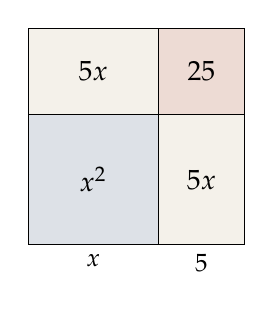
\begin{tikzpicture}[scale=0.55]
\fill[tief!15] (0,0) rectangle (3,3); \node at (1.5,1.5) {$x^{2}$};
\fill[sand] (3,0) rectangle (5,3); \node at (4,1.5) {$5x$};
\fill[sand] (0,3) rectangle (3,5); \node at (1.5,4) {$5x$};
\fill[akzent!20] (3,3) rectangle (5,5); \node at (4,4) {$25$};
\draw (0,0) rectangle (5,5); \draw (3,0)--(3,5); \draw (0,3)--(5,3);
\node[below,font=\small] at (1.5,0) {$x$}; \node[below,font=\small] at (4,0) {$5$};
\end{tikzpicture}
\end{center}
Das Quadrat $x^{2}$ und die zehn Wurzeln $10x$, als zwei Rechtecke $5\times x$ an zwei Seiten angelegt, haben zusammen die Fläche $39$. Das Eckquadrat $5\times5 = 25$ ergänzt die Figur zum großen Quadrat mit Seite $x + 5$ und Fläche $39 + 25 = 64$. Also $x + 5 = 8$, $x = 3$.
\schritt{Modern}
$x^{2} + 10x + 25 = 64$, $(x + 5)^{2} = 64$, $x = -5\pm8$. Die Lösung $-13$ hat in der Figur keinen Platz.
\probe{$9 + 30 = 39$. \checkmark}
\begin{mitnehmen}\kastentext
\enquote{Quadratische Ergänzung} ist wörtlich gemeint: Eine Figur wird zum Quadrat ergänzt. Al-Chwarizmi gibt das Rezept \emph{und} die Begründung --- das unterscheidet ihn von den Babyloniern (Aufgabe 7.6), die dasselbe Rezept hatten. Die Begründung ist griechisch (Euklid II.4), das Rezept babylonisch, die Verbindung seine.
\end{mitnehmen}
\end{loesungkarte}

%%%%%%%%%% 7.21
\stupserzwei{gruen}{Parabel $x^{2} = 2y$, Kreis $(x - 1)^{2} + y^{2} = 1$. Einsetzen von $y = \frac{x^{2}}2$: $x^{2} - 2x + \frac{x^{4}}4 = 0$, durch $x$: $\frac{x^{3}}4 + x - 2 = 0$, mal $4$: $x^{3} + 4x = 8$.}{22pt}
\begin{loesungkarte}{gruen}{7.21}{Chayyams Kegelschnitte}
\derweg{Parabel mit Parameter $p = \sqrt a$, Kreis mit Durchmesser $b/a$ auf der Achse; der Schnittpunkt erfüllt die kubische Gleichung.}
\schritt{Umformung}
$x^{3} + ax = b$ mit $a = p^{2}$, $p = 2$: $x^{3} + p^{2}x = b$. Chayyam denkt in Proportionen: Gesucht ist $x$ mit $x^{3} = p^{2}(\frac b{p^{2}} - x)$, also $x^{2} : p^{2} = (\frac b{p^{2}} - x) : x$ --- wenn wir $\frac b{p^{2}} = 2$ setzen.
\schritt{Parabel und Kreis}
Parabel $x^{2} = py$, hier $x^{2} = 2y$: Für ihre Punkte ist $y = \frac{x^{2}}p$. Kreis mit Durchmesser $\frac b{p^{2}} = \frac84 = 2$ auf der $x$-Achse von $0$ bis $2$: $(x - 1)^{2} + y^{2} = 1$, also $y^{2} = x(2 - x)$. Im Schnittpunkt: $\frac{x^{4}}{p^{2}} = x(2 - x)$, $x^{3} = p^{2}(2 - x) = 8 - 4x$. \checkmark
\schritt{Zahl}
$x^{3} + 4x - 8 = 0$: $f(1{,}36) = 2{,}515 + 5{,}44 - 8 = -0{,}045$, $f(1{,}37) = 2{,}571 + 5{,}48 - 8 = 0{,}051$. Newton: $x = 1{,}36466$. Der Schnittpunkt liegt bei $(1{,}365;\ 0{,}931)$.
\schritt{Was Chayyam hatte und nicht hatte}
Er zeigt: Die Lösung existiert und ist konstruierbar (als Strecke, mit Kegelschnitten). Er findet keine Zahl und keine Formel; er schreibt, er hoffe auf Nachfolger, die sie finden --- das waren del Ferro und Tartaglia (Aufgabe 7.24), $450$ Jahre später. Und er sieht nur die positive Lösung.
\probe{$1{,}36466^{3} + 4\cdot1{,}36466 = 2{,}5414 + 5{,}4586 = 8{,}0000$. \checkmark}
\begin{mitnehmen}\kastentext
Chayyam klassifizierte alle kubischen Gleichungen (mit positiven Koeffizienten: $14$ Typen) und gab zu jedem die Kegelschnitte. Es ist die erste systematische Theorie der Gleichungen dritten Grades --- geometrisch, weil die Algebra der Zeit nicht reichte. Descartes' \emph{Géométrie} tut $1637$ dasselbe mit Koordinaten.
\end{mitnehmen}
\end{loesungkarte}

%%%%%%%%%% 7.22
\stupserzwei{tief}{$\frac{q^{2}}4 - \frac{p^{3}}{27} = 4 - 125 = -121$. Bombelli: $\sqrt[3]{2 + 11i} + \sqrt[3]{2 - 11i} = (2 + i) + (2 - i) = 4$.}{22pt}
\begin{loesungkarte}{tief}{7.22}{Bombelli und die Wurzel aus $-121$}
\derweg{Lösungen prüfen; Cardano anwenden und die negative Wurzel stehen lassen; mit \enquote{più di meno} weiterrechnen wie mit Zahlen.}
\schritt{(a)}
$64 = 60 + 4$. \checkmark\ Polynomdivision $x^{3} - 15x - 4 = (x - 4)(x^{2} + 4x + 1)$, also $x = -2\pm\sqrt3$. Drei reelle Lösungen.
\schritt{(b)}
$p = 15$, $q = 4$: $\frac{q^{2}}4 - \frac{p^{3}}{27} = 4 - 125 = -121$. $x = \sqrt[3]{2 + \sqrt{-121}} + \sqrt[3]{2 - \sqrt{-121}}$. Cardano hätte gesagt: unmöglich --- und doch ist $x = 4$ eine ganz gewöhnliche Lösung.
\schritt{(c)}
$(2 + i)^{3} = 8 + 3\cdot4\cdot i + 3\cdot2\cdot i^{2} + i^{3} = 8 + 12i - 6 - i = 2 + 11i = 2 + \sqrt{-121}$. Ebenso $(2 - i)^{3} = 2 - 11i$. Also $x = (2 + i) + (2 - i) = 4$. Bombelli schrieb $i$ als \emph{più di meno} (\enquote{plus von minus}) und gab Rechenregeln: \emph{più di meno} mal \emph{più di meno} ist \emph{meno} --- $i\cdot i = -1$. Er rechnete damit, ohne zu wissen, was es ist.
\schritt{(d)}
\emph{Casus irreducibilis}: drei reelle Lösungen, aber die Formel geht durch komplexe Zahlen. Man kann ihn nicht auf reelle Wurzelausdrücke \enquote{zurückführen}: Wantzel bewies $1843$, dass bei drei reellen irrationalen Lösungen \emph{jede} Wurzelformel komplexe Zwischenwerte braucht. Die komplexen Zahlen sind hier nicht Bequemlichkeit, sondern Notwendigkeit.
\probe{Die anderen beiden Lösungen aus Cardano: $\omega(2 + i) + \bar\omega(2 - i) = 2\operatorname{Re}\bigl(\omega(2 + i)\bigr)$ mit $\omega = e^{2\pi i/3}$. $\omega(2 + i) = (-\tfrac12 + \tfrac{\sqrt3}2i)(2 + i) = -1 - \tfrac{\sqrt3}2 + (\sqrt3 - \tfrac12)i$, also $x = -2 - \sqrt3$; mit $\bar\omega$ entsprechend $-2 + \sqrt3$. \checkmark}
\begin{mitnehmen}\kastentext
Die komplexen Zahlen wurden nicht erfunden, um $x^{2} = -1$ zu lösen --- das hielt man für unmöglich und ließ es sein. Sie wurden erfunden, weil man sie für \emph{reelle} Lösungen \emph{brauchte}. Erst Euler ($i$, $1777$), Gauß (Zahlenebene, $1831$) und Hamilton (Zahlenpaare, $1837$) machten aus Bombellis Rechenregeln Zahlen.
\end{mitnehmen}
\end{loesungkarte}

%%%%%%%%%% 7.23
\stupserzwei{gruen}{Monate $1$ bis $12$: $1$, $1$, $2$, $3$, $5$, $8$, $13$, $21$, $34$, $55$, $89$, $144$. Fibonacci zählt den Startmonat mit und kommt im Monat $13$ auf $233$; ohne den Start sind es $144$ \emph{neue} Monate.}{22pt}
\begin{loesungkarte}{gruen}{7.23}{Fibonaccis Kaninchen}
\derweg{Modellannahmen, Rekursion aus \enquote{alte Paare plus Nachwuchs der reifen Paare}, Tabelle, Quotienten.}
\schritt{Modell}
Jedes Paar wird nach einem Monat reif, wirft danach jeden Monat ein Paar, keines stirbt, die Fortpflanzung ist synchron. Unrealistisch in allem --- aber es ist eine Rechenübung, keine Biologie.
\schritt{Rekursion}
$F_n$ Paare im Monat $n$: die $F_{n-1}$ des Vormonats plus ein Neugeborenes je Paar, das im Monat $n - 2$ schon da war (nur die sind reif): $F_n = F_{n-1} + F_{n-2}$, $F_1 = F_2 = 1$.
\schritt{Tabelle}
$1$, $1$, $2$, $3$, $5$, $8$, $13$, $21$, $34$, $55$, $89$, $144$. Nach zwölf Monaten $144$ Paare; Fibonacci selbst zählt den Anfangsmonat als nullten und gibt $377$ (nach $13$ Verdopplungen inklusive des ersten Wurfs) --- je nach Zählweise $144$, $233$ oder $377$. Die Rekursion ist das Wesentliche.
\schritt{Quotienten}
$\frac{F_{n+1}}{F_n}$: $1;\ 2;\ 1{,}5;\ 1{,}667;\ 1{,}6;\ 1{,}625;\ 1{,}615;\ 1{,}619;\ 1{,}618;\ \dots$ --- abwechselnd über und unter $\varphi = \frac{1 + \sqrt5}2 = 1{,}618034$ (Aufgabe 2.34: Binet). Die Näherungsbrüche des Kettenbruchs $[1; 1, 1, \dots]$ (Aufgabe 7.11).
\probe{$F_{12} = 144 = 12^{2}$ --- die einzige Quadratzahl in der Folge außer $1$ (Cohn 1964). $F_{12} = \frac{\varphi^{12} - \psi^{12}}{\sqrt5} = \frac{321{,}997 + 0{,}003}{2{,}236} = 144{,}0$. \checkmark}
\begin{mitnehmen}\kastentext
Die Folge war in Indien schon bekannt (Silbenmuster in der Metrik, Pingala, um $200$ v.\,Chr.; Hemachandra $1150$). Fibonacci gab ihr eine Aufgabe, Kepler den goldenen Schnitt, Lucas ($1877$) den Namen. Der \emph{Liber abbaci} ist wichtiger für etwas anderes: Er brachte die indisch-arabischen Ziffern nach Europa.
\end{mitnehmen}
\end{loesungkarte}

%%%%%%%%%% 7.24
\stupserzwei{gruen}{$x^{3} + 6x = 20$: $p = 6$, $q = -20$. $u^{3}, v^{3}$ sind die Lösungen von $z^{2} + 20z - 8 = 0$: $-10\pm\sqrt{108}$. $x = \sqrt[3]{\sqrt{108} + 10} - \sqrt[3]{\sqrt{108} - 10} = 2$.}{22pt}
\begin{loesungkarte}{gruen}{7.24}{Cardanos Formel}
\derweg{$x = u + v$, Nebenbedingung $3uv = -p$ wählen, dann sind $u^{3}, v^{3}$ Lösungen einer quadratischen Gleichung.}
\schritt{Ansatz}
$x = u + v$: $(u + v)^{3} + p(u + v) + q = u^{3} + v^{3} + 3uv(u + v) + p(u + v) + q = u^{3} + v^{3} + (3uv + p)(u + v) + q$.
\schritt{Nebenbedingung}
Eine Unbekannte wurde durch zwei ersetzt --- also darf man eine Bedingung frei wählen: $3uv = -p$. Dann bleibt $u^{3} + v^{3} = -q$, und $u^{3}v^{3} = -\frac{p^{3}}{27}$.
\schritt{Vieta}
$u^{3}$ und $v^{3}$ sind Lösungen von $z^{2} + qz - \frac{p^{3}}{27} = 0$: $z = -\frac q2\pm\sqrt{\frac{q^{2}}4 + \frac{p^{3}}{27}}$. Also
\[ x = \sqrt[3]{-\frac q2 + \sqrt{\frac{q^{2}}4 + \frac{p^{3}}{27}}} + \sqrt[3]{-\frac q2 - \sqrt{\frac{q^{2}}4 + \frac{p^{3}}{27}}}. \]
\schritt{Cardanos Beispiel}
$x^{3} + 6x - 20 = 0$: $p = 6$, $q = -20$. $\frac{q^{2}}4 + \frac{p^{3}}{27} = 100 + 8 = 108$. $x = \sqrt[3]{10 + \sqrt{108}} + \sqrt[3]{10 - \sqrt{108}} = \sqrt[3]{20{,}392} + \sqrt[3]{-0{,}392} = 2{,}732 - 0{,}732 = 2$. Cardano schreibt das Ergebnis in Wurzeln und bemerkt, es sei $2$ --- Probe: $8 + 12 = 20$. \checkmark
\schritt{Die anderen Lösungen}
$x^{3} + 6x - 20 = (x - 2)(x^{2} + 2x + 10)$, $x = -1\pm3i$: komplex. Für Cardano gab es sie nicht; sein Beispiel ist so gewählt, dass die Wurzel positiv ist und keine Komplikation auftritt.
\probe{$\sqrt[3]{10 + \sqrt{108}} = 1 + \sqrt3$: $(1 + \sqrt3)^{3} = 1 + 3\sqrt3 + 9 + 3\sqrt3 = 10 + 6\sqrt3 = 10 + \sqrt{108}$. \checkmark\ Und $\sqrt[3]{10 - \sqrt{108}} = 1 - \sqrt3$; Summe $2$. \checkmark}
\begin{mitnehmen}\kastentext
Der Trick --- Freiheit durch eine überflüssige Unbekannte --- ist allgemein: Man führt mehr Variablen ein, als man braucht, und wählt die Nebenbedingung so, dass sich etwas vereinfacht. Dieselbe Idee steckt in der Variation der Konstanten (Band 14) und in Lagrange-Multiplikatoren (Aufgabe 3.49). Die Formel selbst ist in der Praxis selten nützlich: Numerik (Aufgabe 5.23) ist schneller.
\end{mitnehmen}
\end{loesungkarte}

%%%%%%%%%% 7.25
\stupserzwei{gruen}{$\log3{,}472 = 0{,}5406$, $\log2{,}718 = 0{,}4343$, Summe $0{,}9749$, Antilog $9{,}438$. Exakt $9{,}437$.}{22pt}
\begin{loesungkarte}{gruen}{7.25}{Napiers Logarithmen}
\derweg{Das Prinzip aus der Funktionalgleichung; Napiers kinematische Definition; zwei Rechnungen mit Tafelwerten.}
\schritt{Prinzip}
Eine Funktion mit $\log(ab) = \log a + \log b$ verwandelt Multiplikation in Addition: Tafel nachschlagen, addieren, zurückschlagen. Entsprechend $\log\sqrt[n]a = \frac1n\log a$: Wurzeln werden Divisionen.
\schritt{Napiers Definition}
Zwei Punkte starten gleichzeitig: Einer läuft mit konstanter Geschwindigkeit auf einer unendlichen Geraden, der andere auf einer Strecke der Länge $10^{7}$ mit einer Geschwindigkeit, die proportional zum verbleibenden Weg ist. Der Logarithmus von $x$ (dem Restweg) ist der Weg des ersten Punkts: $\mathrm{NapLog}(x) = 10^{7}\ln\frac{10^{7}}x$. Kein $e$, keine Basis --- $e$ steckt in der Differentialgleichung $\dot x = -x$ versteckt. $\mathrm{NapLog}(ab)$ ist \emph{nicht} $\mathrm{NapLog}(a) + \mathrm{NapLog}(b)$, sondern erfüllt eine ähnliche Regel mit Korrekturterm; Briggs ($1617$) richtete die Tafel mit $\log1 = 0$, $\log10 = 1$ ein.
\schritt{Produkt}
$\log3{,}472 = 0{,}5406$, $\log2{,}718 = 0{,}4343$ (vierstellige Tafel). Summe $0{,}9749$. Antilogarithmus $10^{0{,}9749} = 9{,}438$. Exakt $3{,}472\cdot2{,}718 = 9{,}437$. Fehler in der vierten Stelle --- vierstellige Logarithmen geben etwa vier Stellen.
\schritt{Wurzel}
$\log1234 = 3{,}0913$; durch $3$: $1{,}0304$; Antilog $10{,}73$. Exakt $\sqrt[3]{1234} = 10{,}726$. Eine Kubikwurzel ohne Logarithmen hätte Iteration gekostet; mit Tafel sind es zwei Nachschlagen und eine Division.
\probe{Die Fehlergrenze: Tafelwerte auf $\pm5\cdot10^{-5}$, also relative Fehler des Ergebnisses etwa $\ln10\cdot10^{-4} = 2\cdot10^{-4}$ --- $9{,}438$ gegen $9{,}437$ passt. \checkmark}
\begin{mitnehmen}\kastentext
Logarithmen waren $350$ Jahre das Rechenwerkzeug --- Tafeln, Rechenschieber, Rechenstab. Kepler rechnete damit die Rudolfinischen Tafeln, Laplace sagte, sie hätten das Leben der Astronomen verdoppelt. Dass $\ln$ die Umkehrung von $e^{x}$ ist, kam später (Euler $1748$); Napier hatte eine Kinematik, Briggs eine Tabelle, beide ohne Exponentialfunktion.
\end{mitnehmen}
\end{loesungkarte}

%%%%%%%%%% 7.26
\stupserzwei{tief}{$x^{2} + (y - c)^{2} = r^{2}$ mit $x^{2} = y$: $y^{2} + (1 - 2c)y + c^{2} - r^{2} = 0$. Doppelte Nullstelle bei $y = 1$: $(y - 1)^{2} = y^{2} - 2y + 1$, also $1 - 2c = -2$, $c = \frac32$.}{22pt}
\begin{loesungkarte}{tief}{7.26}{Descartes' Normalenmethode}
\derweg{Kreis um $(0, c)$ mit der Kurve schneiden; Berührung heißt doppelte Nullstelle; Koeffizientenvergleich gibt $c$; die Normale ist die Verbindung zum Mittelpunkt.}
\schritt{Ansatz}
Kreis mit Mittelpunkt $(0, c)$ durch $(1, 1)$: $x^{2} + (y - c)^{2} = 1 + (1 - c)^{2}$. Auf der Parabel ist $x^{2} = y$: $y + (y - c)^{2} = 1 + (1 - c)^{2}$, also $y^{2} + (1 - 2c)y + c^{2} - 1 - (1 - c)^{2} = 0$, also $y^{2} + (1 - 2c)y + 2c - 2 = 0$.
\schritt{Berührung}
Der Kreis berührt die Parabel in $(1, 1)$ genau dann, wenn $y = 1$ doppelte Nullstelle ist: $y^{2} + (1 - 2c)y + 2c - 2 = (y - 1)^{2} = y^{2} - 2y + 1$. Vergleich: $1 - 2c = -2$, also $c = \frac32$; und $2c - 2 = 1$. \checkmark
\schritt{Normale und Tangente}
Normale: von $(1, 1)$ zum Mittelpunkt $(0, \frac32)$, Richtung $(-1, \frac12)$, Steigung $-\frac12$. Tangente senkrecht dazu: Steigung $2$. Ableitung: $y' = 2x = 2$ bei $x = 1$. \checkmark
\schritt{Warum unhandlich}
Für $y = x^{3}$ im Punkt $(1, 1)$ entsteht mit $y = x^{3}$ eine Gleichung sechsten Grades in $x$, die bei $x = 1$ eine doppelte Nullstelle haben soll --- der Koeffizientenvergleich wird lang. Für transzendente Kurven (Zykloide, Spirale) gibt es keine algebraische Gleichung, und die Methode versagt ganz. Fermats und Newtons Zugang über Differenzenquotienten (Aufgabe 7.27) ist allgemein und kurz --- aber nicht algebraisch rein.
\probe{Der Kreis $x^{2} + (y - \frac32)^{2} = \frac54$: bei $x = 1$, $y = 1$: $1 + \frac14 = \frac54$. \checkmark\ Schmiegkreis der Parabel bei $(1, 1)$ hat Radius $5{,}59$ (Aufgabe 6.27), Descartes' Kreis $1{,}12$ --- er berührt, schmiegt sich aber nicht an.}
\begin{mitnehmen}\kastentext
Descartes wollte Tangenten ohne Infinitesimalien: \enquote{Berührung $=$ doppelte Nullstelle} ist rein algebraisch und völlig streng --- und genau deshalb auf algebraische Kurven beschränkt. Der Streit Descartes--Fermat ($1638$) über Tangentenmethoden ist der Streit zwischen algebraischer Strenge und analytischer Reichweite; die Analysis gewann, und ihre Strenge kam erst $200$ Jahre später nach.
\end{mitnehmen}
\end{loesungkarte}

%%%%%%%%%% 7.27
\stupserzwei{gruen}{$bx - x^{2}\approx bx - x^{2} + be - 2xe - e^{2}$; also $be - 2xe - e^{2}\approx0$; durch $e$: $b - 2x - e\approx0$; $e$ weglassen: $x = \frac b2$.}{22pt}
\begin{loesungkarte}{gruen}{7.27}{Fermats Adäqualität}
\derweg{$f(x)$ und $f(x + e)$ adäqual setzen, vereinfachen, durch $e$ teilen, $e$ streichen.}
\schritt{Ansatz}
Teile $x$ und $b - x$, Rechteck $f(x) = x(b - x) = bx - x^{2}$. Fermat: In der Nähe des Maximums sind $f(x)$ und $f(x + e)$ \enquote{adäqual} (ungefähr gleich): $bx - x^{2}\approx b(x + e) - (x + e)^{2} = bx - x^{2} + be - 2xe - e^{2}$.
\schritt{Vereinfachen}
Gleiche Terme weg: $0\approx be - 2xe - e^{2}$. Durch $e$ teilen: $0\approx b - 2x - e$. Nun $e$ streichen (\enquote{weglassen}): $b - 2x = 0$, $x = \frac b2$. Das Rechteck ist das Quadrat.
\schritt{Berkeleys Einwand}
Erst teilt man durch $e$ --- also ist $e\neq0$. Dann setzt man $e = 0$. Berkeley ($1734$, gegen Newton): Das seien \enquote{Geister verstorbener Größen}. Fermat sagt \enquote{adäqual}, nicht \enquote{gleich}, und das ist ehrlicher als Leibniz' Gleichheitszeichen (Aufgabe 7.32) --- aber eine Definition von \enquote{adäqual} gibt er nicht.
\schritt{Modern}
$\frac{f(x + e) - f(x)}e = b - 2x - e\to b - 2x$ für $e\to0$: Der Grenzwert des Differenzenquotienten ist null im Extremum. Fermats Rechnung ist genau diese, mit $\approx$ statt $\lim$. Er hat die Ableitung und die notwendige Bedingung $f' = 0$ --- ohne beide Begriffe.
\probe{$f(\frac b2) = \frac{b^{2}}4$; $f(\frac b2\pm e) = \frac{b^{2}}4 - e^{2}$: Die Änderung ist zweiter Ordnung in $e$ --- das ist der Grund, warum \enquote{adäqual} funktioniert. \checkmark}
\begin{mitnehmen}\kastentext
Fermat ($1636$) fand auch Tangenten so und wusste, dass Maximum und Tangente dieselbe Rechnung sind. Was fehlte: der Grenzwert als Begriff, der \enquote{durch $e$ teilen, dann $e = 0$} rechtfertigt. Cauchy lieferte ihn $1821$ --- bis dahin rechnete man zweihundert Jahre richtig mit einer unbegründeten Methode.
\end{mitnehmen}
\end{loesungkarte}

%%%%%%%%%% 7.28
\stupserzwei{gruen}{Vier Verläufe der nächsten zwei Runden: $AA, AB, BA, BB$. In dreien gewinnt $A$. Also $\frac34\cdot64 = 48$ für $A$, $16$ für $B$.}{22pt}
\begin{loesungkarte}{gruen}{7.28}{Das Teilungsproblem}
\derweg{Fermat: alle gleich wahrscheinlichen Verläufe zählen. Pascal: vom sicheren Anteil rückwärts. Beide: Es zählt die Zukunft, nicht die Vergangenheit.}
\schritt{Fermat}
$A$ braucht noch einen Sieg, $B$ zwei. Spätestens nach zwei Runden ist entschieden. Fermats Kunstgriff: Man denkt sich beide Runden gespielt, auch wenn die zweite oft nicht mehr nötig ist --- dann sind alle vier Verläufe $AA, AB, BA, BB$ gleich wahrscheinlich. $A$ gewinnt in $AA, AB, BA$: $P(A) = \frac34$. Aufteilung $48 : 16$.
\schritt{Pascal}
Rückwärts: Beim Stand $2 : 2$ wäre die Lage symmetrisch, jeder bekäme $32$. Beim Stand $2 : 1$: Gewinnt $A$ die nächste Runde, erhält er $64$; verliert er, steht es $2 : 2$ und er erhält $32$. In jedem Fall mindestens $32$ --- die gehören ihm sicher. Um die übrigen $32$ wird mit gleichen Chancen gespielt: je $16$. $A$: $32 + 16 = 48$. --- Das ist der Erwartungswert $\frac12\cdot64 + \frac12\cdot32 = 48$, ein Begriff, den Pascal hier erstmals verwendet.
\schritt{Pacioli}
$2 : 1$ teilt nach den \emph{gewonnenen} Runden --- der Vergangenheit. Aber der Einsatz gehört dem, der das Spiel gewonnen \emph{hätte}, und das hängt von den \emph{ausstehenden} Runden ab. Beim Stand $2 : 0$ gäbe Pacioli alles an $A$, obwohl $B$ noch mit $\frac18$ gewinnen kann (drei Siege in Folge); beim Stand $1 : 0$ gäbe er auch alles an $A$ --- absurd.
\probe{Stand $2 : 0$: $B$ braucht drei Siege: $P(B) = \frac18$, $A$ erhält $56$. Stand $1 : 0$: $A$ braucht zwei, $B$ drei; von vier Runden gewinnt $A$, wenn er mindestens zwei gewinnt: $\frac{11}{16}$, also $44$. \checkmark}
\begin{mitnehmen}\kastentext
Der Briefwechsel Pascal--Fermat ($1654$) ist die Geburtsurkunde der Wahrscheinlichkeitsrechnung: Fermats Abzählen gleich wahrscheinlicher Fälle ist Laplace' Definition (Aufgabe 4.1), Pascals Rückwärtsrechnen ist die Methode des ersten Schritts (Aufgabe 4.34). Und die Einsicht, dass die Zukunft zählt, ist die Grundlage jeder Bewertung von Optionen.
\end{mitnehmen}
\end{loesungkarte}

%%%%%%%%%% 7.29
\stupserzwei{tief}{(b) Fehler von $\pi$ nach $n$ Gliedern $< \frac4{2n + 1}$. Für $0{,}005$: $n > 400$. Für $5\cdot10^{-11}$: $n > 4\cdot10^{10}$.}{22pt}
\begin{loesungkarte}{tief}{7.29}{Die Leibniz-Reihe}
\derweg{Geometrische Reihe gliedweise integrieren; Leibniz-Fehlerschranke; Machins Formel mit kleinen Argumenten.}
\schritt{(a)}
$\frac1{1 + t^{2}} = 1 - t^{2} + t^{4} - \dots$ für $|t| < 1$; gliedweise integriert: $\arctan x = x - \frac{x^{3}}3 + \frac{x^{5}}5 - \dots$ Bei $x = 1$ (Rand des Konvergenzbereichs, Abelscher Grenzwertsatz): $\frac\pi4 = 1 - \frac13 + \frac15 - \dots$
\schritt{(b)}
Alternierend mit fallenden Gliedern: Fehler $< $ erstes weggelassenes Glied $\frac1{2n + 1}$; für $\pi$ mal $4$. Zwei Nachkommastellen ($< 0{,}005$): $\frac4{2n + 1} < 0{,}005$, $n > 400$. Zehn Stellen: $n > 4\cdot10^{10}$ --- bei einer Million Gliedern pro Sekunde elf Stunden. Mit $400$ Gliedern: $3{,}1391$ (Fehler $0{,}0025$). \checkmark
\schritt{(c)}
$\arctan\frac15 = 0{,}2 - \frac{0{,}008}3 + \frac{0{,}00032}5 - \frac{0{,}0000128}7 = 0{,}2 - 0{,}0026667 + 0{,}0000640 - 0{,}0000018 = 0{,}1973955$ (vier Glieder). $\arctan\frac1{239} = 0{,}0041841 - \frac{7{,}3\cdot10^{-8}}3 = 0{,}0041841$ (zwei Glieder). $\frac\pi4 = 4\cdot0{,}1973955 - 0{,}0041841 = 0{,}7853979$, $\pi = 3{,}141592$ --- sechs Stellen mit sechs Gliedern. (Mit fünf Gliedern für $\arctan\frac15$: $3{,}1415927$.)
\schritt{(d)}
Die Glieder bei $x = \frac15$ fallen wie $\frac1{(2k + 1)25^{k}}$ --- jedes Glied bringt $1{,}4$ Dezimalstellen; bei $x = 1$ fallen sie nur wie $\frac1{2k + 1}$. Der Konvergenzradius ist $1$; am Rand ist die Konvergenz logarithmisch langsam, im Inneren geometrisch schnell. Machins Kunst war, $\frac\pi4$ aus Arkustangens \emph{kleiner} Argumente zusammenzusetzen.
\probe{Machins Identität: $\tan(4\arctan\frac15) = \frac{120}{119}$ (zweimal Doppelwinkel), und $\tan(\arctan\frac{120}{119} - \arctan\frac1{239}) = \frac{120/119 - 1/239}{1 + 120/(119\cdot239)} = \frac{28\,561}{28\,561} = 1$. \checkmark}
\begin{mitnehmen}\kastentext
Leibniz' Reihe ist schön, weil sie $\pi$ mit den ungeraden Zahlen verbindet (Madhava kannte sie $300$ Jahre früher, mit Korrekturtermen). Zum Rechnen taugt sie nicht; Machin-Formeln rechneten $\pi$ bis $1949$ ($2037$ Stellen, ENIAC), danach übernahmen AGM-Verfahren (Aufgabe 7.15) und Ramanujans Reihen.
\end{mitnehmen}
\end{loesungkarte}

%%%%%%%%%% 7.30
\stupserzwei{akzent}{(c) $\sum(-1)^{n}x^{n} = \frac1{1 + x}$ für $|x| < 1$; $\lim_{x\to1^{-}}\frac1{1 + x} = \frac12$. Die Abel-Summe ist $\frac12$ --- Eulers Wert, als Grenzwert richtig gelesen.}{22pt}
\begin{loesungkarte}{akzent}{7.30}{Was Euler durfte}
\derweg{Divergenz über Partialsummen; die falschen Gleichungen in richtige Grenzwertaussagen übersetzen; Abel-Summation als die Regel, die Euler fehlte.}
\schritt{(a)}
Partialsummen $1, 0, 1, 0, \dots$: keine Konvergenz. Klammern: $(1 - 1) + (1 - 1) + \dots = 0$, aber $1 - (1 - 1) - (1 - 1) - \dots = 1$. Grandi ($1703$) schloss daraus auf die Schöpfung aus dem Nichts; Euler schloss auf $\frac12$ --- als Mittel, und weil $\frac1{1 + x}$ bei $x = 1$ gleich $\frac12$ ist.
\schritt{(b)}
$1 - 2 + 3 - 4 + \dots$: Partialsummen $1, -1, 2, -2, \dots$, divergent. $1 + 2 + 4 + \dots$: divergiert gegen $+\infty$; $-1$ ist absurd als Summe. Richtig gemeint: Die Funktionen $\frac1{(1 + x)^{2}}$ und $\frac1{1 - x}$ setzen die Potenzreihen über ihren Konvergenzkreis hinaus fort (analytische Fortsetzung); der Wert der \emph{Funktion} an der Stelle ist $\frac14$ bzw.\ $-1$. Die \emph{Reihe} hat dort keinen Wert. Euler verwechselte Funktion und Reihe --- und hatte bei der Funktion immer recht.
\schritt{(c)}
Abel-Summe von $\sum a_n$: $\lim_{x\to1^{-}}\sum a_nx^{n}$, falls existent. Für $a_n = (-1)^{n}$: $\sum(-1)^{n}x^{n} = \frac1{1 + x}\to\frac12$. Abelscher Grenzwertsatz: Konvergiert $\sum a_n$ gegen $s$, so ist auch die Abel-Summe $s$ --- die Methode ist \emph{regulär}, sie widerspricht der gewöhnlichen Summe nie. Sie erweitert sie nur auf manche divergente Reihen ($1 - 1 + 1 - \dots$, $1 - 2 + 3 - \dots$), nicht auf alle ($1 + 2 + 4 + \dots$ hat auch keine Abel-Summe; $x = 2$ liegt außerhalb).
\schritt{(d)}
Regel: Eine Potenzreihe darf man am Randpunkt $x_0$ des Konvergenzkreises auswerten, \emph{wenn die Zahlenreihe dort konvergiert}; dann ist ihr Wert der Grenzwert der Funktion (Abel). Konvergiert sie dort nicht, ist der Funktionswert kein Reihenwert. Euler hatte die Regel nicht und setzte immer ein; Cauchy verbot es; Abel ($1826$) bewies, wann es geht.
\begin{fehler}\kastentext
\enquote{Die Funktion hat bei $x = 1$ den Wert $\frac12$} und \enquote{die Reihe bei $x = 1$ hat die Summe $\frac12$} sind verschiedene Aussagen, und nur die erste ist wahr. Euler nahm die zweite als Definition --- was zulässig ist, wenn man es sagt (Abel-, Cesàro-, Borel-Summation) und unzulässig, wenn man dann mit \enquote{$=$} weiterrechnet wie mit konvergenten Reihen.
\end{fehler}
\begin{mitnehmen}\kastentext
Eulers Instinkt war richtig: Divergente Reihen tragen Information, und es gibt konsistente Regeln, sie zu summieren (Hardy, \emph{Divergent Series}, $1949$). $1 + 2 + 3 + \dots = -\frac1{12}$ ist in diesem Sinn die Zeta-Regularisierung --- physikalisch real im Casimir-Effekt, und als Gleichung zwischen Zahlen falsch.
\end{mitnehmen}
\end{loesungkarte}

%%%%%%%%%% 7.31
\stupserzwei{gruen}{$\sqrt2 = \frac75\sqrt{\frac{50}{49}} = 1{,}4\sqrt{1 + \frac1{49}}$: $1 + \frac1{98} - \frac1{8\cdot49^{2}} + \frac1{16\cdot49^{3}} = 1{,}01015254$; mal $1{,}4$: $1{,}4142136$.}{22pt}
\begin{loesungkarte}{gruen}{7.31}{Newtons Binomialreihe}
\derweg{Binomialkoeffizienten mit $\frac12$ ausrechnen; $x = 1$ ist am Rand, $x = \frac1{49}$ tief im Inneren.}
\schritt{Verallgemeinerung}
$(1 + x)^{\alpha} = \sum\binom\alpha kx^{k}$ mit $\binom\alpha k = \frac{\alpha(\alpha - 1)\cdots(\alpha - k + 1)}{k!}$ --- für ganzes $\alpha$ bricht die Reihe ab (binomischer Satz), für gebrochenes nicht. Newton sah das Muster an den Zwischenzeilen des Pascalschen Dreiecks und vertraute ihm; bewiesen hat es Euler (für rationale $\alpha$) und Abel ($1826$, mit Konvergenzradius $1$).
\schritt{Reihe für $\sqrt{1 + x}$}
$\binom{1/2}1 = \frac12$, $\binom{1/2}2 = \frac{\frac12\cdot(-\frac12)}2 = -\frac18$, $\binom{1/2}3 = \frac{\frac12(-\frac12)(-\frac32)}6 = \frac1{16}$, $\binom{1/2}4 = -\frac5{128}$. $\sqrt{1 + x} = 1 + \frac x2 - \frac{x^{2}}8 + \frac{x^{3}}{16} - \frac{5x^{4}}{128} + \dots$
\schritt{$x = 1$}
$\sqrt2 = 1 + 0{,}5 - 0{,}125 + 0{,}0625 - 0{,}039 + 0{,}027 - \dots$: Die Glieder fallen wie $k^{-3/2}$ --- konvergent, aber nach $100$ Gliedern erst zwei Stellen. Rand des Konvergenzkreises.
\schritt{Newtons Trick}
$\sqrt2 = \sqrt{\frac{49}{25}\cdot\frac{50}{49}} = \frac75\sqrt{1 + \frac1{49}}$. $x = \frac1{49} = 0{,}020408$: $1 + 0{,}0102041 - 0{,}0000521 + 0{,}0000005 - \dots = 1{,}0101525$. Mal $1{,}4$: $1{,}4142135$. Sieben Stellen mit vier Gliedern; jedes weitere Glied bringt etwa $1{,}7$ Stellen.
\probe{$\sqrt2 = 1{,}41421356$. \checkmark\ Newtons Fassung: Er rechnete so Logarithmen auf $50$ Stellen und schämte sich später, \enquote{zu viele Stellen} berechnet zu haben.}
\begin{mitnehmen}\kastentext
Die Binomialreihe war Newtons erstes großes Werkzeug: Mit ihr integrierte er $\sqrt{1 - x^{2}}$ (Kreisfläche, also $\pi$), $\frac1{1 + x}$ (Logarithmus) und fand die Reihen für $\sin$ und $\arcsin$. Und der Trick \enquote{nahe bei einem bekannten Wert entwickeln} ist derselbe wie bei Taylor um $x_0\neq0$ (Aufgabe 3.32).
\end{mitnehmen}
\end{loesungkarte}

%%%%%%%%%% 7.32
\stupserzwei{gruen}{$du\,dv$ ist \enquote{unendlich klein von zweiter Ordnung}: Teilt man durch $dx$, bleibt $\frac{du}{dx}dv$, und $dv\to0$. Der Grenzwert tut, was Leibniz durch Streichen tat.}{22pt}
\begin{loesungkarte}{gruen}{7.32}{Leibniz' Produktregel}
\derweg{Differential des Produkts ausmultiplizieren, das Produkt der Differentiale streichen; dann die drei Rechtfertigungen.}
\schritt{Leibniz}
$d(uv) = (u + du)(v + dv) - uv = u\,dv + v\,du + du\,dv$. Leibniz: $du\,dv$ ist unendlich klein gegenüber $u\,dv$ und $v\,du$ (zweite gegen erste Ordnung) und wird weggelassen: $d(uv) = u\,dv + v\,du$. (In seinem Manuskript von $1675$ probierte er zuerst $d(uv) = du\,dv$ --- und merkte am Beispiel, dass es falsch ist.)
\schritt{Was unstreng ist}
$du$ ist entweder $0$ --- dann ist $d(uv) = 0$, nichts gewonnen --- oder nicht $0$ --- dann darf man $du\,dv$ nicht streichen. Berkeleys Einwand (Aufgabe 7.27). Leibniz antwortete, $du$ sei \enquote{unvergleichlich klein}, wie ein Sandkorn gegen die Erde: eine Analogie, keine Definition.
\schritt{Grenzwert}
$\frac{(u + \Delta u)(v + \Delta v) - uv}{\Delta x} = u\frac{\Delta v}{\Delta x} + v\frac{\Delta u}{\Delta x} + \frac{\Delta u}{\Delta x}\Delta v$. Für $\Delta x\to0$: Die ersten beiden Terme gehen gegen $uv' + vu'$, der dritte gegen $u'\cdot0 = 0$, weil $\Delta v\to0$ (Stetigkeit von $v$). Das Streichen ist ein Grenzübergang, und der dritte Term verschwindet \emph{wirklich}, nicht \enquote{ungefähr}.
\schritt{Nichtstandardanalysis}
Robinson ($1961$): Es gibt Zahlkörper mit echten infinitesimalen Elementen (kleiner als jede positive reelle Zahl, aber $\neq0$). Dort ist $du\,dv$ eine infinitesimale Zahl zweiter Ordnung, und $d(uv)/dx = uv' + vu' + u'\,dv$; der \emph{Standardteil} (die nächste reelle Zahl) ist $uv' + vu'$. Leibniz' Rechnung wird wörtlich richtig --- mit einem Schlussschritt, dem Standardteil, den er \enquote{Streichen} nannte.
\probe{$u = v = x$: $d(x^{2}) = x\,dx + x\,dx = 2x\,dx$. \checkmark\ Mit $du\,dv$: $2x\,dx + dx^{2}$, und $\frac{dx^{2}}{dx} = dx\to0$. \checkmark}
\begin{mitnehmen}\kastentext
Leibniz' Kalkül war richtig, bevor er begründet war --- $150$ Jahre lang. Die Begründung kam dreimal: Cauchy/Weierstraß (Grenzwerte, $1821$--$1870$), Robinson (Infinitesimalien, $1961$), und die glatte Infinitesimalanalysis (Lawvere, $1970$er). Alle drei sagen: Leibniz hatte recht, und sein $du\,dv$ darf weg.
\end{mitnehmen}
\end{loesungkarte}

%%%%%%%%%% 7.33
\stupserzwei{gruen}{Koeffizient von $x^{2}$ im Produkt: $-\sum\frac1{n^{2}\pi^{2}}$. In der Reihe: $-\frac16$. Also $\sum\frac1{n^{2}} = \frac{\pi^{2}}6$.}{22pt}
\begin{loesungkarte}{gruen}{7.33}{Das Basler Problem}
\derweg{$\sin x$ wie ein Polynom über seine Nullstellen faktorisieren; Koeffizientenvergleich mit der Taylorreihe.}
\schritt{Die Idee}
Ein Polynom mit $p(0) = 1$ und Nullstellen $r_1, \dots, r_n$ ist $p(x) = \prod\bigl(1 - \frac x{r_i}\bigr)$. Euler behandelt $\frac{\sin x}x$ (Wert $1$ bei $0$, Nullstellen $\pm\pi, \pm2\pi, \dots$) genauso:
\[ \frac{\sin x}x = \prod_{n\ge1}\Bigl(1 - \frac x{n\pi}\Bigr)\Bigl(1 + \frac x{n\pi}\Bigr) = \prod_{n\ge1}\Bigl(1 - \frac{x^{2}}{n^{2}\pi^{2}}\Bigr). \]
\schritt{Koeffizientenvergleich}
Links: $\frac{\sin x}x = 1 - \frac{x^{2}}6 + \frac{x^{4}}{120} - \dots$ Rechts, ausmultipliziert bis $x^{2}$: $1 - \Bigl(\sum_{n\ge1}\frac1{n^{2}\pi^{2}}\Bigr)x^{2} + \dots$ Vergleich: $\frac1{\pi^{2}}\sum\frac1{n^{2}} = \frac16$, also $\sum_{n\ge1}\frac1{n^{2}} = \frac{\pi^{2}}6 = 1{,}644934$.
\schritt{Die Lücke}
Warum darf man eine unendliche Reihe wie ein Polynom faktorisieren? Ein Polynom ist durch Nullstellen und Leitkoeffizient bestimmt; $e^{x}\cdot\frac{\sin x}x$ hat dieselben Nullstellen und denselben Wert bei $0$. Euler brauchte, dass es keine solche \enquote{versteckte} Funktion gibt --- das ist der Produktsatz von Weierstraß ($1876$), und für $\sin$ stimmt es, weil $\sin$ \enquote{langsam wächst} (Ordnung $1$). Euler wusste, dass hier etwas fehlte, und gab $1741$ einen zweiten Beweis.
\schritt{Numerische Probe}
Euler hatte vorher die Summe mit Beschleunigungstricks auf $20$ Stellen berechnet: $1{,}64493406684822643647$. Dann fand er die Formel und prüfte: $\frac{\pi^{2}}6 = 1{,}64493406684822643647$. Übereinstimmung auf $20$ Stellen --- das überzeugte ihn und alle anderen, bevor der Beweis stand.
\probe{Koeffizient von $x^{4}$: $\frac1{120} = \frac1{\pi^{4}}\sum_{m < n}\frac1{m^{2}n^{2}}$, woraus mit $\bigl(\sum\frac1{n^{2}}\bigr)^{2} = \sum\frac1{n^{4}} + 2\sum_{m < n}$ folgt: $\sum\frac1{n^{4}} = \frac{\pi^{4}}{90}$. Euler rechnete so bis $\zeta(26)$. \checkmark}
\begin{mitnehmen}\kastentext
Eulers Lösung ist das Muster für \enquote{kühne Analogie, numerisch geprüft, später bewiesen}. Die Werte $\zeta(2k)$ sind alle rationale Vielfache von $\pi^{2k}$; über $\zeta(3)$ weiß man nur, dass es irrational ist (Apéry $1978$). Die Riemannsche Zetafunktion (Band 10) beginnt mit dieser Reihe.
\end{mitnehmen}
\end{loesungkarte}

%%%%%%%%%% 7.34
\stupserzwei{tief}{(b) $r' = r + \frac{2 - r^{2}}{r + 2} = \frac{2r + 2}{r + 2}$; $2 - r'^{2} = \frac{2(2 - r^{2})}{(r + 2)^{2}} > 0$. Also $r' > r$ und $r'\in A$.}{22pt}
\begin{loesungkarte}{tief}{7.34}{Ein Dedekind-Schnitt}
\derweg{Die drei Schnitteigenschaften prüfen; dann zeigen, dass weder $A$ ein Maximum noch $B$ ein Minimum hat --- das ist die Lücke, die $\sqrt2$ heißt.}
\schritt{(a)}
$0\in A$, $2\in B$ (da $4 > 2$): beide nichtleer; $2$ ist obere Schranke von $A$. Ist $a\in A$, $b\in B$, so $a\le0 < b$ oder ($a > 0$ und $a^{2} < 2\le b^{2}$, also $a < b$, da beide positiv). Jedes $a$ ist kleiner als jedes $b$: ein Schnitt.
\schritt{(b)}
Sei $r\in A$, $r > 0$, $r^{2} < 2$. Setze $r' = \frac{2r + 2}{r + 2}$. Dann $r' - r = \frac{2r + 2 - r^{2} - 2r}{r + 2} = \frac{2 - r^{2}}{r + 2} > 0$, also $r' > r$. Und $2 - r'^{2} = \frac{2(r + 2)^{2} - (2r + 2)^{2}}{(r + 2)^{2}} = \frac{2r^{2} + 8r + 8 - 4r^{2} - 8r - 4}{(r + 2)^{2}} = \frac{4 - 2r^{2}}{(r + 2)^{2}} = \frac{2(2 - r^{2})}{(r + 2)^{2}} > 0$, also $r'\in A$. Kein Element von $A$ ist das größte.
\schritt{(c)}
Dieselbe Formel: Für $r\in B$ ($r > 0$, $r^{2} > 2$) ist $r' < r$ und $r'^{2} > 2$, also $r'\in B$ und kleiner. Kein kleinstes Element. --- Die Lücke: $A$ hat kein Supremum in $\mathbb Q$ (es müsste das größte Element von $A$ oder das kleinste von $B$ sein). In $\mathbb R$ \emph{definiert} Dedekind: Die reelle Zahl $\sqrt2$ \emph{ist} dieser Schnitt. Das Supremum von $A$ in $\mathbb R$ ist der Schnitt selbst.
\schritt{(d)}
$A' = \{r < 1\}$, $B' = \{r\ge1\}$: $B'$ hat ein kleinstes Element, $1$. Dieser Schnitt \enquote{ist} die rationale Zahl $1$; es klafft keine Lücke. Rationale Zahlen sind Schnitte, bei denen eine Klasse ein Randelement hat; irrationale sind Schnitte ohne. Zusammen bilden alle Schnitte $\mathbb R$ --- und das Vollständigkeitsaxiom (jede beschränkte Menge hat ein Supremum) wird zum Satz.
\probe{$r = 1$: $r' = \frac43 = 1{,}333$; $r'' = \frac{14/3}{10/3} = 1{,}4$; $r''' = \frac{4{,}8}{3{,}4} = 1{,}4118$; weiter $1{,}4138$, $1{,}41416$ --- von unten gegen $\sqrt2$. \checkmark\ (Die Iteration $r\mapsto\frac{2r + 2}{r + 2}$ ist der Kettenbruch $[1; 2, 2, 2, \dots]$, Aufgabe 7.11.)}
\begin{mitnehmen}\kastentext
Dedekind ($1858$ gefunden, $1872$ veröffentlicht): Eine reelle Zahl ist eine Lücke in $\mathbb Q$ --- oder ein rationaler Punkt. Das ist Eudoxos' Proportionenlehre (Euklid V, Def.\ 5) in moderner Form; Dedekind sagt es selbst. Damit stand die Analysis erstmals auf den natürlichen Zahlen, ohne Geometrie und ohne Anschauung.
\end{mitnehmen}
\end{loesungkarte}

%%%%%%%%%% 7.35
\stupserzwei{gruen}{Gliedweise abgeleitet: $-\sum a^{n}b^{n}\pi\sin(b^{n}\pi x)$ mit $(ab)^{n}\to\infty$: Die Summanden werden \emph{größer}, nicht kleiner. Das ist der Grund, warum die Ableitung scheitert --- und noch kein Beweis.}{22pt}
\begin{loesungkarte}{gruen}{7.35}{Die Weierstraß-Funktion}
\derweg{Stetigkeit über gleichmäßige Konvergenz; Nichtdifferenzierbarkeit über Differenzenquotienten, die mit $(ab)^{n}$ wachsen.}
\schritt{Stetig}
$|a^{n}\cos(b^{n}\pi x)|\le a^{n}$, und $\sum a^{n} = \frac1{1 - a} < \infty$. Weierstraß' Majorantenkriterium: Die Reihe konvergiert gleichmäßig; eine gleichmäßig konvergente Reihe stetiger Funktionen ist stetig (Aufgabe 3.45). Fertig --- die Stetigkeit ist die leichte Hälfte.
\schritt{Nicht differenzierbar: die Idee}
Der $n$-te Summand schwingt mit Frequenz $b^{n}$ und Amplitude $a^{n}$; seine Steigung ist bis zu $a^{n}b^{n}\pi = (ab)^{n}\pi$. Da $ab > 1$, werden die Steigungen mit $n$ \emph{größer}. Eine Ableitung müsste der Grenzwert der Differenzenquotienten sein; aber auf jeder Skala $h\approx b^{-n}$ dominiert der $n$-te Summand den Differenzenquotienten mit einem Beitrag der Größe $(ab)^{n}$, der mit wechselndem Vorzeichen gegen $\pm\infty$ geht. Die Bedingung $ab > 1 + \frac{3\pi}2$ stellt sicher, dass die Summanden $> n$ den $n$-ten nicht auslöschen; $b$ ungerade sorgt für die richtigen Vorzeichen. (Hardy $1916$: $ab\ge1$ genügt.)
\schritt{Bild}
Die Funktion sieht in jeder Vergrößerung gleich zackig aus --- ein Fraktal (Band 8), Dimension zwischen $1$ und $2$. Es gibt keine Stelle, an der sie \enquote{lokal gerade} ist.
\probe{$a = \frac12$, $b = 13$: $ab = 6{,}5 > 1 + 4{,}71$. \checkmark\ Die Partialsummen $S_N$ sind glatt; ihre Ableitung bei $x = 0$ ist $0$ für alle $N$ (alle Kosinus haben dort ein Maximum) --- aber $\frac{W(h) - W(0)}h$ für $h = b^{-N}$ ist von der Größe $-(ab)^{N}$: Die Grenzprozesse $N\to\infty$ und $h\to0$ vertauschen nicht. \checkmark}
\begin{mitnehmen}\kastentext
Bolzano hatte $1830$ ein ähnliches Beispiel (unveröffentlicht), Riemann vermutete eines, Weierstraß bewies es $1872$. Die Reaktion --- Hermite: \enquote{Ich wende mich mit Schrecken und Entsetzen ab} --- zeigt, wie sehr die Anschauung die Analysis geführt hatte. Danach gilt: Jeder Satz braucht die Voraussetzung, die er braucht, und \enquote{stetig} ist nicht \enquote{fast differenzierbar}.
\end{mitnehmen}
\end{loesungkarte}

%%%%%%%%%% 7.36
\stupserzwei{gruen}{Bei $\mathbb Q$ bricht es an der letzten Stelle: Die Diagonalzahl ist konstruiert, aber nichts garantiert, dass sie \emph{rational} ist --- und sie ist es im Allgemeinen nicht.}{22pt}
\begin{loesungkarte}{gruen}{7.36}{Cantors Diagonale}
\derweg{Annahme einer Liste, Diagonalzahl mit Ziffernwechsel, Widerspruch; dann die zwei Feinheiten.}
\schritt{Annahme}
$[0, 1]$ sei abzählbar: eine Liste $x_1, x_2, x_3, \dots$ enthält alle. Schreibe $x_k = 0{,}a_{k1}a_{k2}a_{k3}\dots$ als Dezimalbruch (bei zwei Darstellungen die ohne Neunerperiode).
\schritt{Diagonale}
Definiere $y = 0{,}b_1b_2b_3\dots$ mit $b_k = 4$, falls $a_{kk}\neq4$, und $b_k = 5$, falls $a_{kk} = 4$. Dann ist $b_k\neq a_{kk}$ für jedes $k$.
\schritt{Widerspruch}
$y\in[0, 1]$, also $y = x_k$ für ein $k$. Dann stimmen alle Ziffern überein, insbesondere $b_k = a_{kk}$. Widerspruch. Keine Liste enthält alle: $[0, 1]$ ist überabzählbar. $\blacksquare$
\schritt{Warum nicht für $\mathbb Q$}
Für $\mathbb Q$ gibt es eine Liste (Cantors erstes Diagonalverfahren, Band 10). Das Argument lässt sich formal durchführen und liefert eine Zahl $y$, die nicht in der Liste steht --- aber $y$ ist dann eben nicht rational; es ist eine irrationale Zahl, deren Ziffern aus der Liste gebastelt wurden. Der Widerspruch braucht, dass $y$ zur Menge gehört, und das gilt für $[0, 1]$ (jede Ziffernfolge ist eine reelle Zahl), nicht für $\mathbb Q$.
\schritt{Neunerperioden}
$0{,}4999\ldots = 0{,}5$: Zwei Ziffernfolgen, eine Zahl. Wäre $y$ eine Neunerperiode, könnte es mit einem $x_k$ übereinstimmen, obwohl die Ziffern verschieden sind. Deshalb wählt man $b_k\in\{4, 5\}$: $y$ enthält weder $0$ noch $9$ und hat eine eindeutige Darstellung. Ein Detail, das in populären Fassungen fehlt --- und ohne das der Beweis eine Lücke hat.
\probe{Variante mit Binärfolgen: Die Menge aller $0$-$1$-Folgen ist überabzählbar (dasselbe Argument mit $b_k = 1 - a_{kk}$, hier ohne das Periodenproblem, wenn man Folgen statt Zahlen nimmt). Und $|\mathcal P(\mathbb N)| > |\mathbb N|$: Cantors Satz (Aufgabe 7.40). \checkmark}
\begin{mitnehmen}\kastentext
Das Diagonalargument ist eine Maschine: Aus jeder Liste von Objekten baut sie ein Objekt, das an der $k$-ten Stelle vom $k$-ten abweicht. Dieselbe Maschine beweist Cantors Satz, Gödels Unvollständigkeit, Turings Unentscheidbarkeit des Halteproblems und Russells Antinomie --- vier Jahrhundertresultate mit einem Trick.
\end{mitnehmen}
\end{loesungkarte}

%%%%%%%%%% 7.37
\stupserzwei{tief}{(c) Unter zyklischen Vertauschungen wird $t$ mit $\omega$ oder $\omega^{2}$ multipliziert, $t^{3}$ bleibt. Unter Transpositionen wird $t$ zu $t' = x_1 + \omega^{2}x_2 + \omega x_3$. $t^{3}$ nimmt zwei Werte an.}{22pt}
\begin{loesungkarte}{tief}{7.37}{Lagranges Resolvente}
\derweg{Symmetrische Ausdrücke in den Wurzeln sind Polynome in den Koeffizienten; die Lösungsformel ist ein Ausdruck, der \emph{fast} symmetrisch ist.}
\schritt{(a)}
Vieta: $x_1 + x_2 = -p$, $x_1x_2 = q$. $(x_1 - x_2)^{2} = (x_1 + x_2)^{2} - 4x_1x_2 = p^{2} - 4q$. Alle drei sind symmetrisch unter $x_1\leftrightarrow x_2$, und der Hauptsatz über symmetrische Polynome sagt: Jedes symmetrische Polynom in den Wurzeln ist ein Polynom in den Koeffizienten. Deshalb lassen sie sich ohne Kenntnis der Wurzeln ausrechnen.
\schritt{(b)}
$x_1 - x_2$ wechselt unter der Vertauschung das Vorzeichen --- nicht symmetrisch, also kein Polynom in $p, q$. Aber sein Quadrat ist symmetrisch: $x_1 - x_2 = \pm\sqrt{p^{2} - 4q}$. Mit $x_1 + x_2 = -p$: $x_1 = \frac{-p + \sqrt{p^{2} - 4q}}2$. Die Mitternachtsformel, hergeleitet aus der Frage, welcher Ausdruck unter Permutationen wie viele Werte annimmt.
\schritt{(c)}
$t = x_1 + \omega x_2 + \omega^{2}x_3$. Zyklische Permutation $(1\,2\,3)$: $t\mapsto x_2 + \omega x_3 + \omega^{2}x_1 = \omega^{2}t$; also $t^{3}\mapsto t^{3}$. Transposition $(2\,3)$: $t\mapsto x_1 + \omega x_3 + \omega^{2}x_2 =: t'$. Unter allen $6$ Permutationen nimmt $t^{3}$ nur die zwei Werte $t^{3}, t'^{3}$ an. Also sind $t^{3} + t'^{3}$ und $t^{3}t'^{3}$ symmetrisch, Polynome in $p, q$; $t^{3}$ und $t'^{3}$ sind Lösungen einer quadratischen Gleichung (der \emph{Resolvente}), und $x_1 = \frac13(t + t' + (x_1 + x_2 + x_3))$. Das ist Cardanos Formel (Aufgabe 7.24) --- erklärt statt gefunden: $u = \frac t3$, $v = \frac{t'}3$.
\schritt{(d)}
Für Grad $4$ gibt es einen Ausdruck mit $3$ Werten (Resolvente dritten Grades) --- Ferrari. Für Grad $5$ bräuchte man einen Ausdruck in fünf Wurzeln, der unter $S_5$ nur $2$, $3$ oder $4$ Werte annimmt. Lagrange fand keinen; Ruffini und Abel bewiesen, dass es keinen gibt (ein Ausdruck mit weniger als $5$ Werten hat $2$ oder $1$, und $2$ Werte reichen nicht). Galois sagte, warum: $S_5$ hat keine passende Kette von Normalteilern (Aufgabe 7.38).
\probe{(c) numerisch für $x^{3} - 15x - 4$ (Aufgabe 7.22): Wurzeln $4, -2+\sqrt3, -2-\sqrt3$; $t = 4 + \omega(-0{,}268) + \omega^{2}(-3{,}732)$; $t^{3} = 27(2 + 11i)$ --- Bombellis Zahl mal $27$. \checkmark}
\begin{mitnehmen}\kastentext
Lagranges \emph{Réflexions} ($1770$) stellen die richtige Frage: nicht \enquote{wie löst man die Gleichung}, sondern \enquote{was tun Permutationen der Wurzeln mit Ausdrücken in ihnen}. Die Antwort heißt Gruppentheorie, und Lagrange hat ihren ersten Satz (Ordnung der Untergruppe teilt Ordnung der Gruppe) genau hier bewiesen.
\end{mitnehmen}
\end{loesungkarte}

%%%%%%%%%% 7.38
\stupserzwei{gruen}{Zwischenkörper: $\mathbb Q(\omega)$ (Grad $2$, zu $A_3$) und die drei Körper $\mathbb Q(\sqrt[3]2\,\omega^{k})$ (Grad $3$, zu den drei Untergruppen der Ordnung $2$).}{22pt}
\begin{loesungkarte}{gruen}{7.38}{Die Galoisgruppe von $x^{3} - 2$}
\derweg{Nullstellen, Zerfällungskörper und sein Grad, Gruppe als Permutationsgruppe der Nullstellen, Normalteilerkette.}
\schritt{Nullstellen}
$x_1 = \sqrt[3]2 = 1{,}2599$, $x_2 = \sqrt[3]2\,\omega$, $x_3 = \sqrt[3]2\,\omega^{2}$ mit $\omega = e^{2\pi i/3} = -\frac12 + \frac{\sqrt3}2i$. Eine reelle, zwei komplexe.
\schritt{Zerfällungskörper}
$K = \mathbb Q(\sqrt[3]2, \omega)$. $[\mathbb Q(\sqrt[3]2) : \mathbb Q] = 3$ ($x^{3} - 2$ irreduzibel, Eisenstein); $\omega\notin\mathbb Q(\sqrt[3]2)\subset\mathbb R$, also $[K : \mathbb Q(\sqrt[3]2)] = 2$. $[K : \mathbb Q] = 6$.
\schritt{Gruppe}
$|\operatorname{Gal}(K/\mathbb Q)| = 6$; jeder Automorphismus permutiert die drei Nullstellen, und verschiedene Automorphismen geben verschiedene Permutationen. Eine Untergruppe von $S_3$ mit $6$ Elementen: $\operatorname{Gal} = S_3$. Erzeuger: $\sigma\colon\sqrt[3]2\mapsto\sqrt[3]2\,\omega$, $\omega\mapsto\omega$ (Ordnung $3$) und $\tau$ = komplexe Konjugation (Ordnung $2$).
\schritt{Auflösbarkeit}
$S_3\supset A_3\supset\{e\}$: $A_3 = \langle\sigma\rangle$ ist Normalteiler vom Index $2$, $A_3\cong\mathbb Z_3$ ist abelsch. Die Faktoren $\mathbb Z_2$, $\mathbb Z_3$ sind zyklisch: $S_3$ ist auflösbar. Die Gleichung ist durch Wurzeln lösbar --- natürlich, $\sqrt[3]2$ steht ja da; aber Galois' Satz sagt es für jede kubische Gleichung, weil jede Untergruppe von $S_3$ auflösbar ist.
\schritt{Zwischenkörper}
Galois-Korrespondenz: Untergruppen $\leftrightarrow$ Zwischenkörper, Index $\leftrightarrow$ Grad. $A_3$ (Index $2$) $\leftrightarrow$ $\mathbb Q(\omega) = \mathbb Q(\sqrt{-3})$. Die drei Untergruppen $\langle\tau\rangle, \langle\sigma\tau\rangle, \langle\sigma^{2}\tau\rangle$ der Ordnung $2$ (Index $3$) $\leftrightarrow$ $\mathbb Q(\sqrt[3]2)$, $\mathbb Q(\sqrt[3]2\,\omega)$, $\mathbb Q(\sqrt[3]2\,\omega^{2})$. Nur $\mathbb Q(\omega)$ ist über $\mathbb Q$ galoissch --- weil nur $A_3$ Normalteiler ist.
\probe{Cardano für $x^{3} - 2 = 0$ ($p = 0$, $q = -2$): $x = \sqrt[3]{1 + 1} + \sqrt[3]{1 - 1} = \sqrt[3]2$. Die Formel \enquote{sieht} die Kette: erst $\sqrt{\dots}$ (zu $\mathbb Q(\omega)$), dann $\sqrt[3]{\dots}$. \checkmark}
\begin{mitnehmen}\kastentext
Galois ($1832$, mit $20$ Jahren, in der Nacht vor dem Duell): Eine Gleichung ist durch Wurzeln lösbar genau dann, wenn ihre Gruppe eine Kette von Normalteilern mit abelschen Faktoren hat. $S_3$ und $S_4$ haben sie, $S_5$ nicht --- deshalb Cardano und Ferrari, und keine Formel für Grad $5$. Band 11 beweist es.
\end{mitnehmen}
\end{loesungkarte}

%%%%%%%%%% 7.39
\stupserzwei{tief}{(c) Induktion über $a$: $0 + 0 = 0$ (Axiom). Gilt $0 + a = a$, so $0 + S(a) = S(0 + a) = S(a)$ (Definition, dann Induktionsannahme).}{22pt}
\begin{loesungkarte}{tief}{7.39}{$2 + 2 = 4$ nach Peano}
\derweg{Alles auf $0$, $S$ und die rekursive Definition der Addition zurückführen; jeden Schritt mit seiner Regel beschriften.}
\schritt{(a)}
Definitionen: $1 := S(0)$, $2 := S(1)$, $3 := S(2)$, $4 := S(3)$. Addition rekursiv: (A1) $a + 0 = a$; (A2) $a + S(b) = S(a + b)$. \\
$2 + 2 = 2 + S(1) \overset{A2}{=} S(2 + 1) = S(2 + S(0)) \overset{A2}{=} S(S(2 + 0)) \overset{A1}{=} S(S(2)) = S(3) = 4$. $\blacksquare$ Vier Schritte, jeder eine Definition oder ein Axiom.
\schritt{(b)}
$a + 1 = a + S(0) \overset{A2}{=} S(a + 0) \overset{A1}{=} S(a)$. $\blacksquare$ Kein Induktionsbeweis nötig --- $a$ bleibt beliebig.
\schritt{(c)}
Induktion über $a$. Anfang: $0 + 0 = 0$ nach (A1). Schritt: Gelte $0 + a = a$. Dann $0 + S(a) \overset{A2}{=} S(0 + a) = S(a)$. $\blacksquare$ --- Das Axiom (A1) sagt $a + 0 = a$ (Null \emph{rechts}); $0 + a = a$ (Null \emph{links}) ist etwas anderes, weil die Addition über das rechte Argument definiert ist. Die Kommutativität $a + b = b + a$ ist ein Satz, der zwei Induktionen braucht.
\schritt{(d)}
Das fünfte Axiom: Enthält eine Menge die $0$ und mit jedem $n$ auch $S(n)$, so enthält sie alle natürlichen Zahlen. Ohne es: Modelle mit \enquote{Nichtstandard-Zahlen}, etwa $\mathbb N\cup\{\dots, \omega - 1, \omega, \omega + 1, \dots\}$ --- eine Kopie von $\mathbb Z$ hinter allen natürlichen Zahlen, die $0$ nie erreicht. Dort gelten die ersten vier Axiome, aber (c) ist nicht mehr beweisbar. Das Induktionsaxiom sagt: Es gibt nur die Zahlen, die man von $0$ aus erreicht.
\probe{$2\cdot2 = 4$ mit (M1) $a\cdot0 = 0$, (M2) $a\cdot S(b) = a\cdot b + a$: $2\cdot2 = 2\cdot1 + 2 = (2\cdot0 + 2) + 2 = (0 + 2) + 2 = 2 + 2 = 4$ --- wobei $0 + 2 = 2$ den Satz (c) braucht. \checkmark}
\begin{mitnehmen}\kastentext
Peano ($1889$; Dedekind $1888$ hatte dieselben Axiome): Fünf Axiome, zwei Definitionen, und die Arithmetik ist ein deduktives System. Russell und Whitehead brauchten in den \emph{Principia Mathematica} $360$ Seiten bis $1 + 1 = 2$ --- weil sie auch die Logik und die Mengen aufbauten. Gödel zeigte $1931$, dass dieses System wahre Sätze hat, die es nicht beweist (Aufgabe 7.40 ist der Anfang dieser Geschichte).
\end{mitnehmen}
\end{loesungkarte}

%%%%%%%%%% 7.40
\stupserzwei{akzent}{(c) $R_M\in R_M$ ist unmöglich (sonst $R_M\notin R_M$); also $R_M\notin R_M$, und dann folgt aus der Definition nur: $R_M\notin M$. Kein Widerspruch --- $R_M$ ist einfach kein Element von $M$.}{22pt}
\begin{loesungkarte}{akzent}{7.40}{Die Menge aller Mengen}
\derweg{Russells Argument; Cantors Satz gegen die Allmenge; wie Aussonderung den Widerspruch in einen harmlosen Satz verwandelt.}
\schritt{(a)}
$R = \{x\colon x\notin x\}$. Für jedes $x$: $x\in R\iff x\notin x$. Setze $x = R$: $R\in R\iff R\notin R$. Eine Aussage ist genau dann wahr, wenn sie falsch ist --- Widerspruch. Also kann es die Menge $R$ nicht geben. Da Cantors (und Freges) Mengenlehre erlaubte, zu \emph{jeder} Eigenschaft die Menge der Dinge mit dieser Eigenschaft zu bilden (Komprehension), ist sie widersprüchlich.
\schritt{(b)}
Cantor: Für jede Menge $M$ ist $|M| < |\mathcal P(M)|$ (Diagonalargument: Zu jeder Abbildung $f\colon M\to\mathcal P(M)$ ist $\{x\colon x\notin f(x)\}$ nicht im Bild). Gäbe es die Menge $V$ aller Mengen, so wäre $\mathcal P(V)\subseteq V$ (jede Teilmenge von $V$ ist eine Menge), also $|\mathcal P(V)|\le|V|$. Widerspruch. --- Cantor kannte dieses Argument ($1899$) und sprach von \enquote{inkonsistenten Vielheiten}.
\schritt{(c)}
Zermelo: Mengen bildet man nur durch Aussonderung aus vorhandenen Mengen, $\{x\in M\colon\varphi(x)\}$. Dann: $R_M = \{x\in M\colon x\notin x\}$. Angenommen $R_M\in R_M$; dann $R_M\in M$ und $R_M\notin R_M$ --- Widerspruch, also $R_M\notin R_M$. Dann aber: Wäre $R_M\in M$, so wäre $R_M\in R_M$ nach Definition --- Widerspruch, also $R_M\notin M$. Kein Paradox, sondern ein Satz: Zu jeder Menge $M$ gibt es eine Menge, die nicht in $M$ liegt. Insbesondere gibt es keine Menge aller Mengen --- bewiesen, nicht widersprüchlich.
\schritt{(d)}
Der Barbier (rasiert genau die, die sich nicht selbst rasieren): Rasiert er sich? Beides führt zum Widerspruch --- also \emph{gibt es keinen solchen Barbier}. Das ist bequem: Niemand hat behauptet, dass es ihn gibt. Bei Mengen ist es unbequem, weil Frege und Cantor behauptet hatten, zu jeder Eigenschaft gebe es die Menge --- und die Antwort \enquote{diese Menge gibt es nicht} verlangt eine neue Regel, welche Mengen es gibt. Das ist die ganze axiomatische Mengenlehre (ZF).
\begin{fehler}\kastentext
\enquote{Die Menge aller $x$ mit \dots} ist nicht automatisch eine Menge. Komprehension ist widersprüchlich; Aussonderung ($\{x\in M\colon\dots\}$ aus einer schon vorhandenen Menge $M$) ist es nicht. Jede Konstruktion \enquote{die Menge aller Mengen, die \dots} braucht die Frage: aus welcher Menge ausgesondert?
\end{fehler}
\begin{mitnehmen}\kastentext
Russell schrieb Frege $1902$; Frege antwortete, die Arithmetik gerate ins Wanken, und fügte seinem zweiten Band ein Nachwort an. Die Antinomie war das Ende der naiven Mengenlehre und der Beginn der Grundlagenkrise --- Zermelo (Axiome, $1908$), Russell (Typentheorie, $1910$), Hilbert (Beweistheorie, $1920$er), Brouwer (Intuitionismus), Gödel ($1931$). Die Mathematik überlebte --- mit expliziten Regeln dafür, was eine Menge ist.
\end{mitnehmen}
\end{loesungkarte}

\cleardoublepage
\setgebiet{9}{Topologie}{mittel}
\chapter{Lösungen: Topologie}

%%%%%%%%%% 8.1
\stupserzwei{tief}{(c) $\frac1p + \frac1q > \frac12$ mit $p, q\ge3$: Ist $p\ge6$, so $\frac1q > \frac12 - \frac16 = \frac13$, also $q < 3$ --- unmöglich. Also $p, q\in\{3, 4, 5\}$, und $(4, 4), (4, 5), (5, 4), (5, 5)$ fallen weg.}{22pt}
\begin{loesungkarte}{tief}{8.1}{Warum es nur fünf platonische Körper gibt}
\derweg{Kanten doppelt zählen, in Euler einsetzen, die entstehende Ungleichung in ganzen Zahlen lösen.}
\schritt{(a)}
Jede der $F$ Flächen hat $p$ Kanten, jede Kante gehört zu genau zwei Flächen: $pF = 2K$. Jede der $E$ Ecken hat $q$ Kanten, jede Kante hat zwei Endpunkte: $qE = 2K$.
\schritt{(b)}
$E = \frac{2K}q$, $F = \frac{2K}p$. Einsetzen: $\frac{2K}q - K + \frac{2K}p = 2$. Durch $2K$: $\frac1q - \frac12 + \frac1p = \frac1K$, also $\frac1p + \frac1q = \frac12 + \frac1K$.
\schritt{(c)}
Da $K > 0$: $\frac1p + \frac1q > \frac12$. Mit $p, q\ge3$: Wäre $p\ge6$, so $\frac1q > \frac13$, also $q\le2$. Also $p\le5$, ebenso $q\le5$. Von den neun Paaren in $\{3, 4, 5\}^{2}$ erfüllen die Ungleichung: $(3, 3)$: $\frac23$; $(3, 4), (4, 3)$: $\frac7{12}$; $(3, 5), (5, 3)$: $\frac8{15}$. Nicht: $(4, 4)$: $\frac12$; $(4, 5), (5, 4)$: $\frac9{20}$; $(5, 5)$: $\frac25$. Genau fünf Lösungen.
\schritt{(d)}
$K = \bigl(\frac1p + \frac1q - \frac12\bigr)^{-1}$:
\begin{center}\small
\begin{tabular}{cc|ccc|l}
$p$ & $q$ & $K$ & $E$ & $F$ & Körper\\ \hline
3 & 3 & 6 & 4 & 4 & Tetraeder\\
4 & 3 & 12 & 8 & 6 & Würfel\\
3 & 4 & 12 & 6 & 8 & Oktaeder\\
5 & 3 & 30 & 20 & 12 & Dodekaeder\\
3 & 5 & 30 & 12 & 20 & Ikosaeder
\end{tabular}
\end{center}
\probe{Würfel: $8 - 12 + 6 = 2$. Ikosaeder: $12 - 30 + 20 = 2$. \checkmark\ Vertauschen von $p$ und $q$ vertauscht $E$ und $F$: Dualität.}
\begin{mitnehmen}\kastentext
Der Beweis benutzt nur $\chi = 2$ und Zählen --- keine Geometrie, keine Winkel. Deshalb gilt er auch für alle \enquote{kombinatorisch regelmäßigen} Zerlegungen der Sphäre. Für den Torus ($\chi = 0$) wird aus der Ungleichung $\frac1p + \frac1q = \frac12$: die drei Parkettierungen der Ebene $(3, 6), (4, 4), (6, 3)$, aufgerollt.
\end{mitnehmen}
\end{loesungkarte}

%%%%%%%%%% 8.2
\stupserzwei{gruen}{$\deg A = 3$, $\deg B = 3$, $\deg C = 5$, $\deg D = 3$. Vier ungerade Knoten --- zwei zu viel.}{22pt}
\begin{loesungkarte}{gruen}{8.2}{Die Brücken von Königsberg}
\derweg{Grade zählen; Paarungsargument an Zwischenknoten; Folgerung; Reparatur.}
\schritt{(a)}
$A$: zwei Brücken nach $C$, eine nach $D$: $3$. $B$: ebenso $3$. $C$: je zwei nach $A$ und $B$, eine nach $D$: $5$. $D$: je eine nach $A, B, C$: $3$. Summe $14 = 2\cdot7$. \checkmark\ (Jede Brücke wird an beiden Enden gezählt --- das \emph{Handschlaglemma}.)
\schritt{(b)}
Sei $W$ ein Weg, der jede Kante genau einmal benutzt, und $v$ ein Knoten, der weder Anfang noch Ende ist. Jedes Mal, wenn $W$ in $v$ ankommt, verlässt er $v$ über eine andere, noch unbenutzte Kante. Die Kanten an $v$ zerfallen also in Paare (Ankunft, Abfahrt): $\deg v$ ist gerade. Nur Anfang und Ende können ungeraden Grad haben (und haben ihn, falls sie verschieden sind). Also höchstens zwei ungerade Knoten. In Königsberg sind es vier: kein solcher Weg. $\blacksquare$
\schritt{(c)}
Reißt man eine Brücke zwischen zwei ungeraden Knoten ab, etwa eine der beiden $A$--$C$-Brücken, so werden $A$ und $C$ gerade ($2$ und $4$); ungerade bleiben $B$ und $D$ --- ein Weg von $B$ nach $D$ existiert dann (Euler zeigte auch die Umkehrung: zusammenhängend mit $0$ oder $2$ ungeraden Knoten genügt). Ebenso hilft eine neue Brücke $A$--$B$ (dann $A, B$ gerade, Weg von $C$ nach $D$). Für einen \emph{Rundweg} müssen alle Grade gerade sein: zwei Brücken abreißen oder bauen, etwa $A$--$B$ und $C$--$D$ neu.
\probe{Nach Abriss einer $A$--$C$-Brücke: $B\to C\to A\to D\to B\to C\to D$ benutzt alle sechs Kanten. \checkmark}
\begin{mitnehmen}\kastentext
Euler hat die Brücken nicht gezeichnet, sondern gezählt --- Lage statt Länge. Das Paaritätsargument ist eine \emph{Invariante}: eine Größe, die jeder Weg hätte, die der Graph aber nicht hat. So beweist man Unmöglichkeit; die Topologie besteht zu großen Teilen aus solchen Invarianten ($\chi$, $\pi_1$, Betti-Zahlen).
\end{mitnehmen}
\end{loesungkarte}

%%%%%%%%%% 8.3
\stupserzwei{gruen}{(b) Vom $4\times4$-Gitter der Eckpunkte bleiben nach dem Verkleben $3\times3 = 9$; von $24$ Kanten $18$; Flächen $9$. $9 - 18 + 9 = 0$.}{22pt}
\begin{loesungkarte}{gruen}{8.3}{Der Torus hat $\chi = 0$}
\derweg{Vor dem Verkleben zählen, dann identifizierte Ecken und Kanten zusammenfassen.}
\schritt{(a)}
Quadrat: $4$ Ecken, $4$ Kanten, $1$ Fläche. Verkleben: Die vier Ecken werden eine (alle sind $(0, 0)\sim(1, 0)\sim(0, 1)\sim(1, 1)$); die Kanten $x = 0$ und $x = 1$ werden eine ($b$), ebenso $y = 0$ und $y = 1$ ($a$). $E = 1$, $K = 2$, $F = 1$: $\chi = 1 - 2 + 1 = 0$.
\schritt{(b)}
$3\times3$-Gitter: $16$ Gitterpunkte, $24$ Kanten ($12$ waagerecht, $12$ senkrecht), $9$ Flächen. Verkleben: Die Randpunkte werden identifiziert --- von $16$ bleiben $9$ (die Eckpunkte des Torus bilden ein $3\times3$-Gitter). Von den $24$ Kanten werden die $3$ unteren mit den $3$ oberen und die $3$ linken mit den $3$ rechten identifiziert: $18$. $\chi = 9 - 18 + 9 = 0$. \checkmark
\schritt{(c)}
Ring aus $n$ Rechtecken: Zylinder mit $2n$ Ecken ($n$ oben, $n$ unten), $3n$ Kanten ($n$ Seitenkanten, $n$ oben, $n$ unten), $n$ Flächen --- $\chi = 2n - 3n + n = 0$ für den Zylinder. Verklebt man die obere mit der unteren Randkurve: $n$ Ecken, $2n$ Kanten, $n$ Flächen: $\chi = 0$ für jedes $n$. \checkmark
\probe{Allgemein: Ein $m\times n$-Gitter auf dem Torus hat $mn$ Ecken, $2mn$ Kanten, $mn$ Flächen --- immer $0$.}
\begin{mitnehmen}\kastentext
$\chi$ hängt nicht von der Zerlegung ab: Jede Verfeinerung (Kante teilen: $+1$ Ecke, $+1$ Kante; Fläche teilen: $+1$ Kante, $+1$ Fläche) lässt $\chi$ unverändert, und je zwei Zerlegungen haben eine gemeinsame Verfeinerung. Die Zahl gehört also zur Fläche, nicht zur Zeichnung --- sie ist die älteste topologische Invariante.
\end{mitnehmen}
\end{loesungkarte}

%%%%%%%%%% 8.4
\stupserzwei{tief}{(a) $B_1(x) = \{x\}$: Jeder Punkt ist offen, also jede Menge. (c) $\arctan$ ist ein Homöomorphismus $\mathbb R\to(-\frac\pi2, \frac\pi2)$; die Metrik ist die von $(-\frac\pi2, \frac\pi2)$ zurückgeholte.}{22pt}
\begin{loesungkarte}{tief}{8.4}{Drei ungewohnte Metriken}
\derweg{Axiome prüfen, dabei die Dreiecksungleichung nach Fällen; Kugeln skizzieren; Topologie ablesen.}
\schritt{(a) Diskrete Metrik}
Nichtnegativ, $d(x, y) = 0\iff x = y$, symmetrisch: nach Definition. Dreiecksungleichung $d(x, z)\le d(x, y) + d(y, z)$: Die linke Seite ist höchstens $1$; die rechte ist $0$ nur für $x = y = z$, und dann ist auch die linke $0$. \checkmark\ Kugeln: $B_r(x) = \{x\}$ für $r\le1$, $B_r(x) = X$ für $r > 1$. Da $\{x\}$ offen ist, ist jede Menge (Vereinigung ihrer Punkte) offen: die \emph{diskrete Topologie}. Jede Abbildung aus einem diskreten Raum ist stetig.
\schritt{(b) Eisenbahnmetrik}
Definitheit und Symmetrie sind klar. Dreiecksungleichung für $x, y, z$: Liegen $x, z$ mit $0$ auf einer Geraden, so ist $d(x, z) = |x - z|\le|x| + |z|$, und $|x| + |z|\le d(x, y) + d(y, z)$ in jedem Fall (ob $y$ nun auf den Geraden liegt oder nicht, ist $d(x, y)\ge\bigl||x| - |y|\bigr|$ bzw.\ $= |x| + |y|$, und man prüft die vier Fälle). Liegen $x, z$ nicht mit $0$ auf einer Geraden: $d(x, z) = |x| + |z|$, und $y$ kann höchstens mit einem der beiden auf einem Strahl durch $0$ liegen; dann ist $d(x, y) + d(y, z)\ge\bigl||x| - |y|\bigr| + |y| + |z|\ge|x| + |z|$. \checkmark\ Kugeln um $x\neq0$: Für $r\le|x|$ ein offenes Stück der Geraden durch $0$ und $x$ (Länge $2r$ um $x$) --- alle anderen Punkte sind mindestens $|x|$ entfernt. Für $r > |x|$: dieses Stück plus die euklidische Kugel vom Radius $r - |x|$ um $0$, deren Punkte man über Paris erreicht.
\schritt{(c) Arctan-Metrik}
$d(x, y) = |\arctan x - \arctan y|$ ist die euklidische Metrik auf dem Bild $(-\frac\pi2, \frac\pi2)$, zurückgeholt mit der Bijektion $\arctan$: alle Axiome übertragen sich. Da $\arctan$ und $\tan$ stetig sind, hat jede Standard-offene Menge eine $d$-Kugel um jeden Punkt und umgekehrt: \emph{dieselben offenen Mengen}. Aber $x_n = n$: $d(n, m) = |\arctan n - \arctan m|\to0$ --- eine Cauchy-Folge ohne Grenzwert ($\arctan n\to\frac\pi2$, und $\frac\pi2$ ist kein $\arctan$). Nicht vollständig.
\probe{(b) Dreiecksungleichung an $x = (1, 0)$, $y = (0, 1)$, $z = (2, 0)$: $d(x, z) = 1\le d(x, y) + d(y, z) = 2 + 3$. \checkmark}
\begin{mitnehmen}\kastentext
(a) zeigt: Die Metrik bestimmt die Topologie, aber verschiedene Metriken können dieselbe Topologie geben --- und eine Metrik kann eine Topologie erzeugen, in der nichts \enquote{nahe} ist. (c) zeigt: Vollständigkeit hängt an der Metrik, nicht an der Topologie (Aufgabe 8.7). (b) zeigt, dass offene Kugeln nicht rund sein müssen --- und dass die Dreiecksungleichung der einzige Punkt ist, an dem man bei neuen Metriken wirklich arbeiten muss.
\end{mitnehmen}
\end{loesungkarte}

%%%%%%%%%% 8.5
\stupserzwei{gruen}{(c) $\max_i|a_i|\le\sqrt{\sum a_i^{2}}\le\sum|a_i|\le n\max_i|a_i|$ --- die erste, weil die Summe den größten Term enthält; die zweite durch Quadrieren; die dritte, weil jeder Term höchstens das Maximum ist.}{22pt}
\begin{loesungkarte}{gruen}{8.5}{Die Maximumsmetrik}
\derweg{Axiome; Einheitskugeln zeichnen; Ungleichungskette; daraus die Gleichheit der Topologien.}
\schritt{(a)}
(M1) Ein Maximum von Beträgen ist $\ge0$ und genau dann $0$, wenn alle $|x_i - y_i| = 0$, also $x = y$. (M2) $|x_i - y_i| = |y_i - x_i|$. (M3) Sei $k$ ein Index mit $d_\infty(x, z) = |x_k - z_k|$. Dann $|x_k - z_k|\le|x_k - y_k| + |y_k - z_k|\le d_\infty(x, y) + d_\infty(y, z)$, weil jeder der beiden Terme höchstens das jeweilige Maximum ist. \checkmark
\schritt{(b)}
\begin{center}
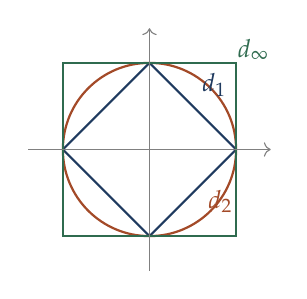
\begin{tikzpicture}[scale=1.1]
\draw[tief,thick] (1,0)--(0,1)--(-1,0)--(0,-1)--cycle;
\draw[akzent,thick] (0,0) circle (1);
\draw[gruen,thick] (-1,-1) rectangle (1,1);
\draw[->,gray] (-1.4,0)--(1.4,0); \draw[->,gray] (0,-1.4)--(0,1.4);
\node[tief,font=\small] at (0.75,0.75) {$d_1$};
\node[akzent,font=\small] at (0.82,-0.6) {$d_2$};
\node[gruen,font=\small] at (1.2,1.15) {$d_\infty$};
\end{tikzpicture}
\end{center}
$d_1$: Raute $|x| + |y|\le1$. $d_2$: Kreis. $d_\infty$: Quadrat $\max(|x|, |y|)\le1$. Raute $\subseteq$ Kreis $\subseteq$ Quadrat.
\schritt{(c)}
Mit $a_i = x_i - y_i$: $\max|a_i|\le\sqrt{\sum a_i^{2}}$, weil $\max|a_i|^{2}$ einer der Summanden ist. $\sqrt{\sum a_i^{2}}\le\sum|a_i|$, weil $\sum a_i^{2}\le\bigl(\sum|a_i|\bigr)^{2}$ (rechts kommen die gemischten Terme $2|a_i||a_j|\ge0$ hinzu). $\sum|a_i|\le n\max|a_i|$. Also $d_\infty\le d_2\le d_1\le n\,d_\infty$. Folglich enthält jede $d_\infty$-Kugel $B^{\infty}_r(x)$ die Kugel $B^{1}_r(x)$, und jede $d_1$-Kugel $B^{1}_r(x)$ die Kugel $B^{\infty}_{r/n}(x)$: Eine Menge, die um jeden Punkt eine Kugel der einen Sorte enthält, enthält auch eine der anderen. Dieselben offenen Mengen. \checkmark
\probe{In $\mathbb R^{2}$: $d_\infty((0,0), (1,1)) = 1$, $d_2 = \sqrt2$, $d_1 = 2 = 2\cdot d_\infty$. Die Kette ist scharf.}
\begin{mitnehmen}\kastentext
Metriken, die sich gegenseitig durch Konstanten abschätzen, heißen \emph{äquivalent} --- sie haben dieselben offenen Mengen, dieselben konvergenten und dieselben Cauchy-Folgen. In $\mathbb R^{n}$ sind alle Normen äquivalent (Band 2); in unendlicher Dimension nicht mehr, und dann beginnt die Funktionalanalysis.
\end{mitnehmen}
\end{loesungkarte}

%%%%%%%%%% 8.6
\stupserzwei{gruen}{(d) $\frac{q^{n}}{1 - q}\cdot0{,}0183 < 10^{-6}$ heißt $0{,}8415^{n} < 8{,}7\cdot10^{-6}$, also $n\ge68$. Tatsächlich ist der Fehler nach $10$ Schritten schon $3{,}4\cdot10^{-5}$.}{22pt}
\begin{loesungkarte}{gruen}{8.6}{$x = \cos x$ mit Banach}
\derweg{Invariantes Intervall; Kontraktion über den Mittelwertsatz; iterieren; a-priori-Schranke auswerten.}
\schritt{(a)}
Für $x\in[0, 1]$ ist $\cos x\in[\cos1, 1] = [0{,}5403, 1]\subseteq[0, 1]$. Enger: $X = [0{,}5, 1]$, denn $\cos$ fällt dort, $\cos(X) = [\cos1, \cos0{,}5] = [0{,}5403, 0{,}8776]\subseteq X$. \checkmark\ $X$ ist abgeschlossen in $\mathbb R$, also vollständig.
\schritt{(b)}
Mittelwertsatz: $|\cos x - \cos y| = |\sin\xi|\,|x - y|$ mit $\xi$ zwischen $x$ und $y$, also $\xi\in X$. Dort ist $\sin$ monoton wachsend, $|\sin\xi|\le\sin1 = 0{,}841471 =: q < 1$. Kontraktion. \checkmark
\schritt{(c)}
$x_1 = \cos0{,}75 = 0{,}731689$, $x_2 = \cos x_1 = 0{,}744047$, $x_3 = 0{,}735734$. Die Folge alterniert um den Grenzwert, weil $\cos' < 0$. Fixpunkt: $x^{*} = 0{,}739085$ (die \emph{Dottie-Zahl}; sie ist transzendent).
\schritt{(d)}
$d(x_1, x_0) = 0{,}018311$. Schranke $\frac{q^{n}}{1 - q}\cdot0{,}018311 = 0{,}1155\cdot0{,}841471^{n}$. Für $n = 10$: $0{,}1155\cdot0{,}178 = 0{,}0206$. Für $< 10^{-6}$: $0{,}841471^{n} < 8{,}66\cdot10^{-6}$, $n > \frac{\ln(8{,}66\cdot10^{-6})}{\ln0{,}841471} = 67{,}5$, also $n = 68$. Tatsächlich: $x_{10} = 0{,}739119$, Fehler $3{,}4\cdot10^{-5}$ --- die Schranke ist um den Faktor $600$ pessimistisch, weil $|\sin\xi|$ nahe $x^{*}$ nur $0{,}674$ ist, nicht $0{,}841$.
\probe{$\cos(0{,}739085) = 0{,}739085$. \checkmark}
\begin{mitnehmen}\kastentext
Banach liefert vier Dinge auf einmal --- Existenz, Eindeutigkeit, Verfahren, Fehlerschranke --- und verlangt dafür nur Vollständigkeit und eine Kontraktion. Die a-priori-Schranke ist grob, aber sie steht \emph{vor} der Rechnung fest. Schneller konvergiert Newton (Aufgabe 5.24), aber ohne eine so bequeme Garantie.
\end{mitnehmen}
\end{loesungkarte}

%%%%%%%%%% 8.7
\stupserzwei{akzent}{(b) Das Bild von $\frac1n$ ist $\tan\bigl(\pi(\frac1n - \frac12)\bigr)\to-\infty$: unbeschränkt, erst recht keine Cauchy-Folge. Der Homöomorphismus erhält Konvergenz, aber nicht \enquote{Cauchy}.}{22pt}
\begin{loesungkarte}{akzent}{8.7}{Vollständigkeit ist nicht topologisch}
\derweg{Homöomorphismus angeben; Cauchy-Folge verfolgen; sortieren, welche Begriffe die Metrik und welche die Topologie brauchen.}
\schritt{(a)}
$h(x) = \tan\bigl(\pi(x - \frac12)\bigr)$ ist stetig und streng monoton von $(0, 1)$ auf $\mathbb R$, mit stetiger Umkehrung $\frac1\pi\arctan y + \frac12$: Homöomorphismus. In $(0, 1)$ ist $\frac1n$ eine Cauchy-Folge (Abstände $\to0$) ohne Grenzwert in $(0, 1)$: nicht vollständig. $\mathbb R$ ist vollständig (Band 3).
\schritt{(b)}
$h(\frac1n) = \tan\bigl(\pi(\frac1n - \frac12)\bigr) = -\cot\frac\pi n\to-\infty$. Keine Cauchy-Folge --- Homöomorphismen erhalten Konvergenz (und Nichtkonvergenz), aber nicht die Cauchy-Eigenschaft, weil diese Abstände vergleicht, die der Homöomorphismus beliebig dehnen darf.
\schritt{(c)}
Beschränkt ist nicht topologisch: $(0, 1)$ beschränkt, $\mathbb R$ nicht, beide homöomorph. Kompakt ist topologisch: definiert über offene Überdeckungen, und ein Homöomorphismus bildet offene Überdeckungen auf offene Überdeckungen ab. In $\mathbb R^{n}$ gilt \enquote{kompakt $=$ abgeschlossen und beschränkt}, aber die rechte Seite ist nur in dieser Kombination topologisch invariant.
\schritt{(d)}
(i) Falsch: $f(x) = \frac1x$ auf $(0, 1)$, $x_n = \frac1n$ Cauchy, $f(x_n) = n$ nicht. (ii) Richtig: Zu $\varepsilon$ gibt es $\delta$ mit $d(x, y) < \delta\Rightarrow d(f(x), f(y)) < \varepsilon$; für $n, m$ groß ist $d(x_n, x_m) < \delta$. (iii) Richtig: Stetige Abbildungen erhalten Konvergenz, $f(x_n)\to f(x)$.
\begin{fehler}\kastentext
\enquote{Vollständig} und \enquote{beschränkt} gehören zur Metrik; \enquote{kompakt}, \enquote{zusammenhängend}, \enquote{offen} zur Topologie. Ein Satz, der \enquote{vollständig} voraussetzt (Banach, Baire), gilt also für einen Raum \emph{mit dieser Metrik}, und ein homöomorpher Raum kann die Voraussetzung verletzen. Umgekehrt: Vollständigkeit lässt sich oft durch Wechsel zu einer äquivalenten Metrik erzwingen --- $(0, 1)$ wird mit $d(x, y) = |h(x) - h(y)|$ vollständig.
\end{fehler}
\begin{mitnehmen}\kastentext
Es gibt eine topologische Fassung: Ein metrisierbarer Raum heißt \emph{vollständig metrisierbar}, wenn \emph{irgendeine} verträgliche Metrik vollständig ist. $(0, 1)$ ist es (via $h$), $\mathbb Q$ nicht (Satz von Baire). Die Frage \enquote{welche Metrik?} ist also keine Spitzfindigkeit, sondern der Unterschied zwischen zwei Begriffen.
\end{mitnehmen}
\end{loesungkarte}

%%%%%%%%%% 8.8
\stupserzwei{gruen}{(b) $[0, 1)$ ist offen (Basiselement) \emph{und} abgeschlossen, denn das Komplement $(-\infty, 0)\cup[1, \infty) = \bigcup_{a < 0}[a, 0)\cup\bigcup_{b > 1}[1, b)$ ist offen.}{22pt}
\begin{loesungkarte}{gruen}{8.8}{Die Sorgenfrey-Gerade}
\derweg{Basiskriterium; Mengen durch Basiselemente ausschöpfen; Vergleich; ein Abzählbarkeitsargument.}
\schritt{(a)}
$\bigcup\mathcal B = \mathbb R$. Durchschnitt: $[a_1, b_1)\cap[a_2, b_2) = [\max a_i, \min b_i)$, wenn nichtleer --- wieder ein Basiselement. Also enthält der Durchschnitt zweier Basiselemente um jeden seiner Punkte ein Basiselement: Basiskriterium erfüllt. \checkmark
\schritt{(b)}
$[0, 1)$: offen (Basiselement), abgeschlossen (siehe Stupser) --- \enquote{abgeschlossen-offen}. $(0, 1) = \bigcup_{n}[\frac1n, 1)$: offen; nicht abgeschlossen (das Komplement enthält $0$, aber kein $[0, \varepsilon)$ liegt im Komplement). $[0, 1]$: abgeschlossen (Komplement $(-\infty, 0)\cup(1, \infty)$ ist in $\mathbb R$ offen, also nach (c) auch hier); nicht offen (kein $[1, b)$ liegt in $[0, 1]$).
\schritt{(c)}
Jedes offene Intervall ist $(a, b) = \bigcup_n[a + \frac1n, b)$, also offen in $\mathbb R_\ell$; damit jede in $\mathbb R$ offene Menge. Umgekehrt ist $[0, 1)$ in $\mathbb R$ nicht offen. $\mathbb R_\ell$ ist echt \emph{feiner} (mehr offene Mengen).
\schritt{(d)}
Sei $\mathcal B'$ irgendeine Basis. Zu jedem $x\in\mathbb R$ gibt es $B_x\in\mathcal B'$ mit $x\in B_x\subseteq[x, x + 1)$. Dann ist $x = \min B_x$. Für $x\neq y$ ist also $B_x\neq B_y$: Die Zuordnung $x\mapsto B_x$ ist injektiv, $\mathcal B'$ hat mindestens die Mächtigkeit von $\mathbb R$ --- überabzählbar. $\blacksquare$ Trotzdem hat jeder Punkt die abzählbare Umgebungsbasis $\{[x, x + \frac1n)\}$: $\mathbb R_\ell$ erfüllt das erste, nicht das zweite Abzählbarkeitsaxiom.
\probe{In $\mathbb R_\ell$ konvergiert $x_n\to x$ genau dann, wenn $x_n\to x$ in $\mathbb R$ und schließlich $x_n\ge x$: $\frac1n\to0$, aber $-\frac1n\not\to0$.}
\begin{mitnehmen}\kastentext
Die Sorgenfrey-Gerade ist separabel ($\mathbb Q$ liegt dicht), erststufig abzählbar, aber nicht zweitstufig --- also nicht metrisierbar (in metrischen Räumen fallen separabel und zweitstufig zusammen). Ihr Quadrat $\mathbb R_\ell\times\mathbb R_\ell$ ist nicht normal. Sie ist das Gegenbeispiel, das man zuerst probiert, wenn eine Vermutung über topologische Räume \enquote{zu gut klingt}.
\end{mitnehmen}
\end{loesungkarte}

%%%%%%%%%% 8.9
\stupserzwei{gruen}{In $\mathbb Q$: $A = \mathbb Q\cap[0, 1]$ ist abgeschlossen (Spur von $[0, 1]$), und offen ist nur $\mathbb Q\cap(0, 1)$ --- um $0$ liegen negative rationale Zahlen.}{22pt}
\begin{loesungkarte}{gruen}{8.9}{Inneres, Abschluss, Rand}
\derweg{Inneres: größte offene Teilmenge. Abschluss: kleinste abgeschlossene Obermenge. Rand: Differenz. In jedem Raum neu.}
\schritt{(a) In $\mathbb R$}
Inneres: Jedes offene Intervall enthält irrationale Zahlen, liegt also nicht in $A$: $\operatorname{int}A = \emptyset$. Abschluss: Jede Umgebung eines $x\in[0, 1]$ enthält rationale Zahlen aus $[0, 1]$, also $[0, 1]\subseteq\overline A$; und $[0, 1]$ ist abgeschlossen: $\overline A = [0, 1]$. Rand: $\partial A = [0, 1]\setminus\emptyset = [0, 1]$.
\schritt{(b) In $\mathbb Q$}
Offen in $\mathbb Q$ sind die Mengen $U\cap\mathbb Q$, $U$ offen in $\mathbb R$. $A = [0, 1]\cap\mathbb Q$ ist abgeschlossen (Spur einer abgeschlossenen Menge): $\overline A = A$. Inneres: $(0, 1)\cap\mathbb Q\subseteq A$ ist offen in $\mathbb Q$; die Punkte $0$ und $1$ haben keine Umgebung in $A$ (jedes $(-\varepsilon, \varepsilon)\cap\mathbb Q$ enthält negative Zahlen). $\operatorname{int}A = (0, 1)\cap\mathbb Q$. Rand: $\partial A = \{0, 1\}$.
\schritt{(c) Diskret}
Jede Menge ist offen und abgeschlossen: $\operatorname{int}A = \overline A = A$, $\partial A = \emptyset$.
\probe{$\partial A = \overline A\setminus\operatorname{int}A$: (a) $[0, 1]\setminus\emptyset$; (b) $A\setminus(0, 1)\cap\mathbb Q = \{0, 1\}$; (c) $A\setminus A = \emptyset$. \checkmark}
\begin{mitnehmen}\kastentext
Dieselbe Punktmenge, drei verschiedene Antworten: Inneres, Abschluss und Rand sind Eigenschaften des Paares (Menge, Raum). Beim Wechsel in einen Teilraum $Y$ gilt $\overline A^{\,Y} = \overline A\cap Y$ --- für das Innere gibt es keine so einfache Regel. Deshalb immer dazusagen: \emph{offen in was?}
\end{mitnehmen}
\end{loesungkarte}

%%%%%%%%%% 8.10
\stupserzwei{akzent}{(d) $\{x\} = \bigcap_n(x - \frac1n, x + \frac1n)$. Wären beliebige Durchschnitte offen, so jede Einpunktmenge --- und damit jede Menge.}{22pt}
\begin{loesungkarte}{akzent}{8.10}{Unendlich viele offene Mengen}
\derweg{Gegenbeispiele in $\mathbb R$; eine Inklusion beweisen, die andere widerlegen.}
\schritt{(a)}
$\bigcap_{n\ge1}(-\frac1n, \frac1n) = \{0\}$: nicht offen. Komplementär: $\bigcup_{n\ge1}[\frac1n, 1] = (0, 1]$: nicht abgeschlossen.
\schritt{(b)}
$\overline{A\cup B} = \overline A\cup\overline B$: \enquote{$\supseteq$}, weil $\overline{A\cup B}$ abgeschlossen ist und $A$, $B$ enthält. \enquote{$\subseteq$}: $\overline A\cup\overline B$ ist abgeschlossen (endliche Vereinigung) und enthält $A\cup B$. Unendlich: $A_n = \{\frac1n\}$, $\overline{A_n} = A_n$, $\bigcup\overline{A_n} = \{\frac1n\colon n\ge1\}$, aber $\overline{\bigcup A_n}$ enthält zusätzlich $0$.
\schritt{(c)}
$\partial(A\cup B)\subseteq\partial A\cup\partial B$: $x\in\partial(A\cup B)$ heißt, jede Umgebung trifft $A\cup B$ und das Komplement $A^{c}\cap B^{c}$. Trifft jede Umgebung $A$, so ist $x\in\partial A$ (denn sie trifft auch $A^{c}$); sonst gibt es eine Umgebung ohne $A$-Punkte, dann treffen alle kleineren $B$, und $x\in\partial B$. Echt: $A = \mathbb Q$, $B = \mathbb R\setminus\mathbb Q$: $\partial A = \partial B = \mathbb R$, $\partial(A\cup B) = \partial\mathbb R = \emptyset$.
\schritt{(d)}
Mit beliebigen Durchschnitten wäre $\{x\} = \bigcap(x - \frac1n, x + \frac1n)$ offen für jedes $x$, also jede Menge als Vereinigung von Punkten offen: die diskrete Topologie. Stetigkeit würde trivial (jede Funktion stetig), Konvergenz bedeutungslos (nur schließlich konstante Folgen konvergieren). Die Beschränkung auf endliche Durchschnitte ist genau das, was \enquote{nahe} von \enquote{gleich} unterscheidet.
\begin{fehler}\kastentext
\enquote{Durchschnitte offener Mengen sind offen} --- nur endliche. \enquote{Vereinigungen abgeschlossener Mengen sind abgeschlossen} --- nur endliche. \enquote{Abschluss der Vereinigung $=$ Vereinigung der Abschlüsse} --- nur endlich. Jeder dieser Sätze ist für unendlich viele Mengen falsch, und der Fehler passiert immer dann, wenn man ein Argument für zwei Mengen \enquote{offensichtlich} auf unendlich viele überträgt.
\end{fehler}
\begin{mitnehmen}\kastentext
Die Asymmetrie der Axiome --- beliebige Vereinigungen, endliche Durchschnitte --- ist kein Zufall: Sie ist das, was in $\mathbb R$ für $\varepsilon$-Umgebungen gilt. Mengen, die abzählbare Durchschnitte offener Mengen sind ($G_\delta$-Mengen, wie $\{0\}$ oder die Irrationalen), bilden eine eigene, wichtige Klasse.
\end{mitnehmen}
\end{loesungkarte}

%%%%%%%%%% 8.11
\stupserzwei{tief}{(b) $x\mapsto\frac x{1 - |x|}$ streckt radial: $|x|\to1$ geht nach $\infty$. Umkehrung $y\mapsto\frac y{1 + |y|}$.}{22pt}
\begin{loesungkarte}{tief}{8.11}{Homöomorphismen hinschreiben}
\derweg{Abbildung, Umkehrabbildung, Stetigkeit beider ablesen (Zusammensetzung stetiger Funktionen, Nenner $\neq0$).}
\schritt{(a)}
$h(x) = \tan\bigl(\pi(x - \frac12)\bigr)$, $h^{-1}(y) = \frac1\pi\arctan y + \frac12$. Für $(a, b)\to(c, d)$: $x\mapsto c + \frac{d - c}{b - a}(x - a)$, affin, Umkehrung affin.
\schritt{(b)}
$h(x) = \frac x{1 - |x|}$ auf $D$: stetig (Nenner $> 0$), $|h(x)| = \frac{|x|}{1 - |x|}$ durchläuft $[0, \infty)$ monoton. Umkehrung $h^{-1}(y) = \frac y{1 + |y|}$, stetig, $|h^{-1}(y)| < 1$. Probe: $h^{-1}(h(x))$: $|h(x)| = \frac{|x|}{1 - |x|}$, $1 + |h(x)| = \frac1{1 - |x|}$, also $\frac{h(x)}{1 + |h(x)|} = x$. \checkmark
\schritt{(c)}
Radialprojektion $h(x) = \frac x{|x|_2}$ vom Quadratrand auf $S^{1}$; Umkehrung $h^{-1}(y) = \frac y{|y|_\infty}$ (Streckung bis zum Quadratrand, wo $\max(|y_1|, |y_2|) = 1$). Beide stetig, weil die Normen stetig und auf den Rändern $\neq0$ sind.
\schritt{(d)}
Stereographische Projektion vom Nordpol $N = (0, 1)$: $h(x, y) = \frac x{1 - y}$ (Schnittpunkt der Geraden durch $N$ und $(x, y)$ mit der $x$-Achse). Umkehrung $h^{-1}(t) = \bigl(\frac{2t}{t^{2} + 1}, \frac{t^{2} - 1}{t^{2} + 1}\bigr)$. Probe: $\bigl(\frac{2t}{t^{2} + 1}\bigr)^{2} + \bigl(\frac{t^{2} - 1}{t^{2} + 1}\bigr)^{2} = \frac{4t^{2} + t^{4} - 2t^{2} + 1}{(t^{2} + 1)^{2}} = 1$. \checkmark\ Für $t\to\pm\infty$ geht $h^{-1}(t)\to N$: $S^{1} = \mathbb R\cup\{\infty\}$, der Nordpol ist der eine fehlende Punkt.
\schritt{(e)}
$h(x) = \bigl(\frac x{|x|}, |x|\bigr)$, Umkehrung $(u, r)\mapsto ru$. Polarkoordinaten, topologisch gelesen: $\mathbb R^{n}\setminus\{0\}\cong S^{n-1}\times(0, \infty)\cong S^{n-1}\times\mathbb R$.
\begin{mitnehmen}\kastentext
Fünf Rezepte: monotone Funktion, radiale Streckung, Radialprojektion, stereographische Projektion, Polarkoordinaten. Fast jeder \enquote{offensichtliche} Homöomorphismus zwischen Teilmengen des $\mathbb R^{n}$ ist eines davon oder eine Zusammensetzung. Und (d) zeigt, dass $S^{n}$ die Einpunktkompaktifizierung von $\mathbb R^{n}$ ist --- der Grund, warum $\infty$ in der Funktionentheorie ein Punkt ist.
\end{mitnehmen}
\end{loesungkarte}

%%%%%%%%%% 8.12
\stupserzwei{gruen}{(d) Quadrat: $4$ Ecken, $4$ Kanten, $1$ Fläche. Verkleben: $(0, 0)\sim(1, 1)$ und $(0, 1)\sim(1, 0)$ --- $2$ Ecken; Kante $a$ verklebt, oben und unten bleiben --- $3$ Kanten. $2 - 3 + 1 = 0$.}{22pt}
\begin{loesungkarte}{gruen}{8.12}{Das Möbiusband}
\derweg{Alles am Quadratmodell $[0, 1]^{2}$, $(0, y)\sim(1, 1 - y)$: Randkanten verfolgen, Schnittlinien verfolgen, Zellen zählen.}
\schritt{(a)}
Vom Quadratrand werden $x = 0$ und $x = 1$ verklebt; es bleiben $y = 0$ und $y = 1$. Die Verklebung verbindet den Endpunkt $(1, 0)$ der unteren Kante mit $(0, 1)$, dem Anfang der oberen, und den Endpunkt $(1, 1)$ der oberen mit $(0, 0)$, dem Anfang der unteren: Die beiden Kanten bilden \emph{eine} geschlossene Kurve. Ein Rand, doppelt so lang wie der Streifen.
\schritt{(b)}
Der Schnitt $y = \frac12$ ist unter $y\mapsto1 - y$ fest: Er trifft sich nach einem Umlauf selbst und schließt sich. Er zerlegt das Quadrat in zwei Streifen $[0, \frac12]$ und $[\frac12, 1]$, die durch die Verklebung über Kreuz verbunden werden: $(0, y)$ mit $y < \frac12$ klebt an $(1, 1 - y)$ mit $1 - y > \frac12$. Also \emph{ein} Band, doppelt so lang, halb so breit. Verfolgt man die Verdrehung: zweimal durch die halbe Drehung, also eine volle Drehung ($360^{\circ}$) pro ursprünglichem Umlauf, und das Band läuft zweimal um --- insgesamt zwei volle Verdrehungen. Zweiseitig, kein Möbiusband.
\schritt{(c)}
Der Schnitt $y = \frac13$ geht bei $x = 1$ über in $y = \frac23$: Die Schnittlinie läuft zweimal um und trennt die Randregion $[0, \frac13]\cup[\frac23, 1]$ (ein Band, zweimal um, zwei Verdrehungen) vom Mittelstreifen $[\frac13, \frac23]$, der mit $y\mapsto1 - y$ verklebt wieder ein Möbiusband ist. Die beiden sind verkettet (die Randregion umschlingt den Mittelstreifen).
\schritt{(d)}
$E = 2$, $K = 3$, $F = 1$: $\chi = 0$. Zylinder ($(0, y)\sim(1, y)$): $E = 2$, $K = 3$, $F = 1$, $\chi = 0$. Torus: $\chi = 0$ (Aufgabe 8.3). Drei Räume mit $\chi = 0$ --- unterschieden durch Rand (Torus: keiner; Zylinder: zwei Komponenten; Möbiusband: eine) und Orientierbarkeit.
\probe{Papier und Schere bestätigen (b) und (c). Die Formel \enquote{Schnitt bei $y = \frac1k$} liefert für jedes $k\ge3$ dasselbe wie (c).}
\begin{mitnehmen}\kastentext
Das Möbiusband ist nicht orientierbar: Ein kleiner Kreispfeil, einmal herumgetragen, kommt gespiegelt zurück. Jede nichtorientierbare Fläche enthält ein Möbiusband --- das ist die Definition, die der Klassifikationssatz benutzt (Aufgabe 8.27). Und $\chi$ allein reicht nicht zur Klassifikation; man braucht $\chi$, Orientierbarkeit und die Zahl der Randkomponenten.
\end{mitnehmen}
\end{loesungkarte}

%%%%%%%%%% 8.13
\stupserzwei{akzent}{(c) Abgeschlossen in kompakt $\Rightarrow$ kompakt; stetiges Bild kompakt; kompakt in Hausdorff $\Rightarrow$ abgeschlossen. Also bildet $f$ abgeschlossene Mengen auf abgeschlossene ab, und $f^{-1}$ ist stetig.}{22pt}
\begin{loesungkarte}{akzent}{8.13}{Stetig und bijektiv, aber kein Homöomorphismus}
\derweg{Zwei Gegenbeispiele; der Satz, der sie ausschließt; eine Anwendung des Satzes.}
\schritt{(a)}
$f$ ist stetig (Komponenten stetig) und bijektiv auf $S^{1}$ ($t\in[0, 1)$ durchläuft den Winkel $[0, 2\pi)$ genau einmal). $f^{-1}$ ist bei $(1, 0)$ unstetig: Die Punkte $f(1 - \frac1n)$ konvergieren gegen $(1, 0) = f(0)$, aber $f^{-1}$ davon, $1 - \frac1n$, konvergiert gegen $1$, nicht gegen $0$. Alternativ: $f([0, \frac12))$ ist offen in $[0, 1)$, sein Bild (ein halber Kreis mit einem Endpunkt) nicht offen in $S^{1}$.
\schritt{(b)}
$\operatorname{id}\colon(\mathbb R, \text{diskret})\to(\mathbb R, \text{Standard})$ ist stetig (jede Abbildung aus einem diskreten Raum ist stetig) und bijektiv. Die Umkehrung $\operatorname{id}\colon(\mathbb R, \text{Standard})\to(\mathbb R, \text{diskret})$ ist nicht stetig: $\{0\}$ ist im Ziel offen, im Urbild nicht.
\schritt{(c)}
Sei $f\colon X\to Y$ stetig, bijektiv, $X$ kompakt, $Y$ Hausdorff. Zu zeigen: $f^{-1}$ stetig, d.\,h.\ $f$ bildet abgeschlossene Mengen auf abgeschlossene ab. Sei $A\subseteq X$ abgeschlossen. Dann ist $A$ kompakt (abgeschlossen in kompakt), $f(A)$ kompakt (stetiges Bild), also abgeschlossen in $Y$ (kompakt in Hausdorff). $\blacksquare$ In (a) ist $[0, 1)$ nicht kompakt; in (b) ist $(\mathbb R, \text{diskret})$ nicht kompakt (die Punkte überdecken ohne endliche Teilüberdeckung).
\schritt{(d)}
Gäbe es eine stetige Bijektion $[0, 1]\to S^{1}$, so wäre sie nach (c) ein Homöomorphismus. Entfernt man $\frac12$ aus $[0, 1]$ und sein Bild aus $S^{1}$, bleibt links ein unzusammenhängender, rechts ein zusammenhängender Raum --- Homöomorphismen erhalten aber Zusammenhang. Widerspruch (Aufgabe 8.14a).
\begin{fehler}\kastentext
\enquote{Stetig und bijektiv, also Homöomorphismus} ist der häufigste Fehlschluss der Anfängertopologie. Die Umkehrabbildung muss \emph{eigens} auf Stetigkeit geprüft werden --- es sei denn, der Satz aus (c) greift. In der linearen Algebra über $\mathbb R^{n}$ und in der Analysis monotoner Funktionen auf Intervallen ist er automatisch erfüllt; deshalb fällt der Fehler dort nie auf.
\end{fehler}
\begin{mitnehmen}\kastentext
Der Satz aus (c) ist das Arbeitspferd beim Nachweis von Homöomorphismen: Verklebemodelle (Quadrat $\to$ Torus) sind kompakt, Zielräume meist Hausdorff, und man braucht nur noch eine stetige Bijektion. Deshalb genügt in Aufgabe 8.3 \enquote{das Quadrat wird zum Torus verklebt}, ohne dass man die Umkehrabbildung hinschreibt.
\end{mitnehmen}
\end{loesungkarte}

%%%%%%%%%% 8.14
\stupserzwei{tief}{(c) Zählen Sie Trennpunkte: I und L haben nur Punkte, die in $2$ Teile trennen; T hat einen $3$-Punkt, X einen $4$-Punkt, O keinen Trennpunkt. P hat genau einen Endpunkt --- I hat zwei, O keinen.}{22pt}
\begin{loesungkarte}{tief}{8.14}{Räume durch Zusammenhang unterscheiden}
\derweg{Ein Homöomorphismus $X\to Y$ induziert einen Homöomorphismus $X\setminus\{p\}\to Y\setminus\{h(p)\}$. Also: Komponenten nach Entfernen von Punkten zählen.}
\schritt{(a)}
Wäre $h\colon[0, 1]\to S^{1}$ ein Homöomorphismus, so auch $[0, 1]\setminus\{\frac12\}\to S^{1}\setminus\{h(\frac12)\}$. Links zwei Komponenten, rechts eine (ein offener Bogen). Widerspruch. $[0, 1]$ und $[0, 1)$: Entfernt man aus $[0, 1)$ den Punkt $0$, bleibt zusammenhängend; aus $[0, 1]$ kann man nur $0$ oder $1$ entfernen, ohne zu trennen. $h(0)$ müsste also $0$ oder $1$ sein --- beides geht: $h(0) = 0$ erlaubt. Dann $h\colon(0, 1]\to(0, 1)$ Homöomorphismus; entferne $1$ links: $(0, 1)$ zusammenhängend; rechts $(0, 1)\setminus\{h(1)\}$ unzusammenhängend. Widerspruch. (Kürzer: $[0, 1]$ ist kompakt, $[0, 1)$ nicht.)
\schritt{(b)}
$\mathbb R\setminus\{0\}$ hat zwei Komponenten; $\mathbb R^{2}\setminus\{p\}$ ist wegzusammenhängend (zwei Punkte verbindet man durch einen Weg, der $p$ umgeht --- etwa über einen dritten Punkt nicht auf ihrer Verbindungsgeraden). Also nicht homöomorph. (Für $\mathbb R^{2}$ gegen $\mathbb R^{3}$ reicht Zusammenhang nicht mehr; man braucht $\pi_1$ oder Homologie.)
\schritt{(c)}
Für jeden Raum zählen wir, wie viele Komponenten nach Entfernen eines Punkts bleiben:
\begin{center}\small
\begin{tabular}{l|P{7.6cm}}
I, L & innere Punkte: $2$; die zwei Endpunkte: $1$\\
T & Verzweigungspunkt: $3$; drei Endpunkte: $1$; sonst $2$\\
X & Verzweigungspunkt: $4$; vier Endpunkte: $1$; sonst $2$\\
O & jeder Punkt: $1$\\
P & Ansatzpunkt: $2$; ein Endpunkt: $1$; Bogenpunkte: $1$; Stielpunkte: $2$
\end{tabular}
\end{center}
I $\cong$ L (ein Bogen, gebogen oder nicht). T, X, O sind untereinander und von I verschieden ($3$-Punkt, $4$-Punkt, kein Trennpunkt). P ist von allen verschieden: Es hat genau \emph{einen} Endpunkt (Punkt, dessen Entfernung nicht trennt und der eine Umgebung homöomorph zu $[0, 1)$ hat) --- I hat zwei, O keinen, T drei; und P hat unendlich viele nichttrennende Punkte, I nur zwei. Fünf Klassen: $\{$I, L$\}$, $\{$T$\}$, $\{$X$\}$, $\{$O$\}$, $\{$P$\}$.
\schritt{(d)}
$g(x) = f(x) - f(-x)$ ist stetig auf $S^{1}$ mit $g(-x) = -g(x)$. Ist $g(x_0) = 0$, fertig. Sonst haben $g(x_0)$ und $g(-x_0)$ verschiedene Vorzeichen; $S^{1}$ ist zusammenhängend, also nimmt $g$ (Zwischenwertsatz für zusammenhängende Räume: $g(S^{1})$ ist ein Intervall) den Wert $0$ an. $\blacksquare$ Anwendung: Auf jedem Breitenkreis der Erde gibt es zwei gegenüberliegende Punkte gleicher Temperatur.
\begin{mitnehmen}\kastentext
\enquote{Nicht homöomorph} beweist man nie durch Scheitern beim Suchen einer Abbildung, sondern durch eine Invariante: eine Eigenschaft, die Homöomorphismen erhalten und in der sich die Räume unterscheiden. Zusammenhang nach Punktentfernung ist die billigste; sie trennt die Dimensionen $1$ und $2$, aber nicht $2$ und $3$ --- dafür braucht man die Werkzeuge der Kapitel 8 und 11.
\end{mitnehmen}
\end{loesungkarte}

%%%%%%%%%% 8.15
\stupserzwei{gruen}{(c) Nach $t_0$ ist $\gamma$ im Graphen; die $x$-Koordinate nimmt nach dem Zwischenwertsatz alle kleinen positiven Werte an, darunter solche mit $\sin\frac1x = 1$ und $= -1$. Die $y$-Koordinate springt dann um $2$ --- in beliebig kleiner Nähe von $t_0$.}{22pt}
\begin{loesungkarte}{gruen}{8.15}{Der Sinuskamm}
\derweg{Zusammenhang über den Abschluss, Wegzusammenhang über einen Widerspruch mit der Stetigkeit am Übergangspunkt.}
\schritt{(a)}
$G$ ist das stetige Bild des Intervalls $(0, 1]$ unter $x\mapsto(x, \sin\frac1x)$, also wegzusammenhängend. Abschluss: Häufungspunkte von $G$ außerhalb $G$ haben $x = 0$; für jedes $y_0\in[-1, 1]$ gibt es $x_n\to0$ mit $\sin\frac1{x_n} = y_0$ (nämlich $\frac1{x_n} = \arcsin y_0 + 2\pi n$), also $(0, y_0)\in\overline G$. Punkte mit $|y| > 1$ oder $x < 0$ liegen nicht im Abschluss. $\overline G = G\cup A = S$. \checkmark
\schritt{(b)}
Der Abschluss einer zusammenhängenden Menge ist zusammenhängend (wäre $\overline G = U\sqcup V$ mit offenen, disjunkten, nichtleeren $U, V$, so läge $G$ ganz in $U$ oder ganz in $V$, etwa in $U$; dann wäre $V\cap\overline G\neq\emptyset$, aber $V$ ist eine offene Umgebung eines Punktes von $\overline G$ ohne Punkte von $G$ --- Widerspruch). Also ist $S$ zusammenhängend.
\schritt{(c)}
Sei $\gamma = (\gamma_1, \gamma_2)\colon[0, 1]\to S$ ein Weg mit $\gamma(0)\in A$, $\gamma(1)\in G$. Die Menge $\gamma^{-1}(A)$ ist abgeschlossen ($A$ abgeschlossen, $\gamma$ stetig), also hat sie ein Maximum $t_0 < 1$. Für $t > t_0$ ist $\gamma(t)\in G$, also $\gamma_1(t) > 0$ und $\gamma_2(t) = \sin\frac1{\gamma_1(t)}$. Stetigkeit bei $t_0$: Es gibt $\delta > 0$ mit $|\gamma_2(t) - \gamma_2(t_0)| < 1$ für $t\in[t_0, t_0 + \delta]$. Auf $(t_0, t_0 + \delta]$ ist $\gamma_1$ stetig und positiv mit $\gamma_1(t)\to0$ für $t\to t_0$; nach dem Zwischenwertsatz nimmt $\gamma_1$ dort jeden Wert in $(0, \gamma_1(t_0 + \delta)]$ an --- insbesondere ein $x'$ mit $\sin\frac1{x'} = 1$ und ein $x''$ mit $\sin\frac1{x''} = -1$. Dann ist $\gamma_2$ an den zugehörigen Stellen $1$ und $-1$, beide im Abstand $< 1$ von $\gamma_2(t_0)$: unmöglich. $\blacksquare$
\schritt{(d)}
$G\cup\{(0, 0)\}$: liegt zwischen $G$ und $\overline G$, also zusammenhängend (dasselbe Argument wie (b)); nicht wegzusammenhängend (dasselbe Argument wie (c) mit $A = \{(0, 0)\}$). $G\cup(\{0\}\times[-2, 2])$: Vereinigung der zusammenhängenden Mengen $S$ und $\{0\}\times[-2, 2]$ mit gemeinsamen Punkten: zusammenhängend; nicht wegzusammenhängend --- der Weg müsste wieder irgendwo von $x = 0$ in den Graphen wechseln.
\begin{mitnehmen}\kastentext
Wegzusammenhängend $\Rightarrow$ zusammenhängend, nicht umgekehrt; aber für offene Teilmengen des $\mathbb R^{n}$ und für lokal wegzusammenhängende Räume fallen beide zusammen. Der Sinuskamm ist nicht lokal wegzusammenhängend bei den Punkten von $A$: Jede kleine Umgebung zerfällt in unendlich viele Streifen. Das ist die Eigenschaft, die der Zwischenwertsatz in (c) ausnutzt.
\end{mitnehmen}
\end{loesungkarte}

%%%%%%%%%% 8.16
\stupserzwei{tief}{(b) Kompakt: $\{0\}\cup\{\frac1n\}$, $S^{n-1}$. Nicht kompakt: $\{\frac1n\}$ (nicht abgeschlossen), Hyperbel (unbeschränkt), Halbscheibe ohne Durchmesser (nicht abgeschlossen), $\mathbb Q\cap[0, 1]$ (nicht abgeschlossen).}{22pt}
\begin{loesungkarte}{tief}{8.16}{Kompakt oder nicht?}
\derweg{Überdeckungen für \enquote{nein}; Heine--Borel für \enquote{ja}; zwei kurze Beweise.}
\schritt{(a)}
$(0, 1) = \bigcup_{n\ge2}(\frac1n, 1)$: endlich viele davon überdecken nur $(\frac1N, 1)$. $\mathbb Z = \bigcup_{n}(n - \frac12, n + \frac12)$: jedes Intervall enthält genau eine ganze Zahl, endlich viele reichen nie. $[0, \infty) = \bigcup_n(-1, n)$.
\schritt{(b)}
Heine--Borel: kompakt $\iff$ abgeschlossen und beschränkt. $\{0\}\cup\{\frac1n\}$: beschränkt, abgeschlossen (einziger Häufungspunkt $0$ ist drin): kompakt. $\{\frac1n\}$ ohne $0$: nicht abgeschlossen. $S^{n-1}$: Urbild von $\{1\}$ unter der stetigen Norm, beschränkt: kompakt. Hyperbel $xy = 1$: abgeschlossen (Urbild), unbeschränkt. Halbscheibe mit $y > 0$: nicht abgeschlossen (der Durchmesser fehlt). $\mathbb Q\cap[0, 1]$: nicht abgeschlossen in $\mathbb R$.
\schritt{(c)}
Sei $K$ kompakt, $f$ stetig, $\{U_i\}$ offene Überdeckung von $f(K)$. Dann ist $\{f^{-1}(U_i)\}$ eine offene Überdeckung von $K$; endlich viele reichen, $K\subseteq f^{-1}(U_{i_1})\cup\dots\cup f^{-1}(U_{i_m})$, also $f(K)\subseteq U_{i_1}\cup\dots\cup U_{i_m}$. $\blacksquare$ Satz vom Maximum: $f\colon K\to\mathbb R$ stetig, $K$ kompakt nichtleer. $f(K)$ ist kompakt in $\mathbb R$, also abgeschlossen und beschränkt, enthält also sein Supremum. $\blacksquare$
\schritt{(d)}
Beschränkt: Die Kugeln $B_n(x_0)$, $n\in\mathbb N$, überdecken; endlich viele reichen, also $K\subseteq B_N(x_0)$. Abgeschlossen: Sei $y\notin K$. Zu jedem $x\in K$ gibt es disjunkte Kugeln $B_{r_x}(x)$, $B_{r_x}(y)$ (Hausdorff, Aufgabe 8.19d). Endlich viele $B_{r_{x_i}}(x_i)$ überdecken $K$; der Durchschnitt der zugehörigen $B_{r_{x_i}}(y)$ ist eine offene Umgebung von $y$ ohne Punkte von $K$. Also ist $K^{c}$ offen. $\blacksquare$ (Nur \enquote{Hausdorff} wurde benutzt: kompakt in Hausdorff $\Rightarrow$ abgeschlossen.)
\begin{mitnehmen}\kastentext
Kompaktheit ist \enquote{Endlichkeit im Kleinen}: Alles, was für endliche Mengen gilt (Maximum existiert, gleichmäßig stetig, Überdeckung hat endliche Teilüberdeckung), gilt für kompakte. Heine--Borel macht den Test in $\mathbb R^{n}$ mechanisch; außerhalb des $\mathbb R^{n}$ braucht man die Definition --- oder Folgenkompaktheit, die in metrischen Räumen dasselbe ist.
\end{mitnehmen}
\end{loesungkarte}

%%%%%%%%%% 8.17
\stupserzwei{gruen}{(e) $\frac14 = 0{,}\overline{02}_3$, $\frac34 = 0{,}\overline{20}_3$, $\frac1{10} = 0{,}\overline{0022}_3$: alle drei ohne Ziffer $1$, alle drei in $C$ --- obwohl keines ein Intervallendpunkt ist.}{22pt}
\begin{loesungkarte}{gruen}{8.17}{Die Cantor-Menge}
\derweg{Kompaktheit über Heine--Borel; Ternärdarstellung als Adresse; Längen summieren; Intervalle und isolierte Punkte ausschließen.}
\schritt{(a)}
$C_n$ ist eine Vereinigung von $2^{n}$ abgeschlossenen Intervallen der Länge $3^{-n}$, also abgeschlossen. $C = \bigcap C_n$ ist abgeschlossen (beliebiger Durchschnitt) und in $[0, 1]$ beschränkt: kompakt. \checkmark
\schritt{(b)}
Im ersten Schritt wird das mittlere Drittel entfernt: die Zahlen, deren erste Ternärziffer $1$ sein \emph{muss} (die Endpunkte $\frac13 = 0{,}1_3 = 0{,}0\overline2_3$ haben eine Alternative und bleiben). Im $n$-ten Schritt: $n$-te Ziffer $1$. Also $x\in C\iff x$ hat eine Ternärdarstellung mit Ziffern aus $\{0, 2\}$. Die Abbildung $0{,}a_1a_2\dots_3\mapsto0{,}b_1b_2\dots_2$ mit $b_i = a_i/2$ ist eine Surjektion von $C$ auf $[0, 1]$ (Binärdarstellungen): $C$ ist überabzählbar --- genauso mächtig wie $[0, 1]$, obwohl es \enquote{fast nichts} ist.
\schritt{(c)}
Entfernt: $1$ Intervall der Länge $\frac13$, dann $2$ der Länge $\frac19$, dann $4$ der Länge $\frac1{27}$, \dots: $\sum_{n\ge0}\frac{2^{n}}{3^{n+1}} = \frac13\cdot\frac1{1 - \frac23} = 1$. Alles. $C$ hat Länge (Lebesgue-Maß) $0$.
\schritt{(d)}
Kein Intervall: Ein Intervall der Länge $\ell > 0$ passt nicht in $C_n$, sobald $3^{-n} < \ell$. Also sind die Zusammenhangskomponenten Punkte: total unzusammenhängend. Kein isolierter Punkt: Ist $x\in C$ mit Ternärziffern $a_i\in\{0, 2\}$, so liegt $x_n$ (dieselben Ziffern, nur $a_n$ durch $2 - a_n$ ersetzt) in $C$ mit $|x - x_n| = 2\cdot3^{-n}\to0$. Jede Umgebung von $x$ enthält andere Punkte von $C$: perfekt.
\schritt{(e)}
$\frac14$: $\frac14\cdot3 = \frac34\to0$; $\frac34\cdot3 = \frac94 = 2 + \frac14\to2$; periodisch $0{,}\overline{02}_3$. Probe: $\frac{2}{9}\cdot\frac1{1 - \frac19} = \frac28 = \frac14$. \checkmark\ $\frac34 = 0{,}\overline{20}_3$. \checkmark\ $\frac1{10}$: $0{,}3\to0$; $0{,}9\to0$; $2{,}7\to2$; $2{,}1\to2$; $0{,}3$ --- Periode $0022$: $\frac1{10} = 0{,}\overline{0022}_3$, Probe $\frac{0\cdot27 + 0\cdot9 + 2\cdot3 + 2}{81 - 1} = \frac8{80}$. \checkmark\ Alle drei in $C$.
\begin{mitnehmen}\kastentext
Die Cantor-Menge widerlegt gleich mehrere Vermutungen: \enquote{überabzählbar $\Rightarrow$ enthält ein Intervall}, \enquote{abgeschlossen ohne isolierte Punkte $\Rightarrow$ positive Länge}, \enquote{Maß null $\Rightarrow$ abzählbar}. Topologisch ist sie $\{0, 2\}^{\mathbb N}$ mit der Produkttopologie --- und jeder kompakte metrische Raum ist ein stetiges Bild von ihr.
\end{mitnehmen}
\end{loesungkarte}

%%%%%%%%%% 8.18
\stupserzwei{akzent}{(c) Jede Kugel vom Radius $\frac12$ enthält höchstens ein $e_n$ (zwei hätten Abstand $\sqrt2 > 1$). Endlich viele Kugeln lassen unendlich viele $e_n$ draußen.}{22pt}
\begin{loesungkarte}{akzent}{8.18}{Die Einheitskugel in $\ell^{2}$}
\derweg{Abgeschlossen und beschränkt nachweisen; dann zwei Beweise der Nichtkompaktheit, über Folgen und über Überdeckungen.}
\schritt{(a)}
Beschränkt: $\|x\|\le1$ nach Definition. Abgeschlossen: $\overline B = \|\cdot\|^{-1}([0, 1])$, Urbild einer abgeschlossenen Menge unter der stetigen Norm (stetig wegen $\bigl|\|x\| - \|y\|\bigr|\le\|x - y\|$).
\schritt{(b)}
$\|e_n - e_m\|^{2} = 1^{2} + (-1)^{2} = 2$, also $\|e_n - e_m\| = \sqrt2$ für $n\neq m$. Eine konvergente Teilfolge wäre eine Cauchy-Folge, deren Glieder schließlich Abstand $< \sqrt2$ hätten --- unmöglich. Keine konvergente Teilfolge: $\overline B$ ist nicht folgenkompakt, in metrischen Räumen also nicht kompakt.
\schritt{(c)}
$\{B_{1/2}(x)\colon x\in\overline B\}$ überdeckt $\overline B$. Jede dieser Kugeln enthält höchstens ein $e_n$: Enthielte sie $e_n$ und $e_m$, so $\sqrt2 = \|e_n - e_m\|\le\|e_n - x\| + \|x - e_m\| < 1$. Endlich viele Kugeln enthalten also nur endlich viele $e_n$, decken $\overline B$ nicht. Keine endliche Teilüberdeckung. \checkmark
\schritt{(d)}
Der Beweis von Heine--Borel halbiert den Würfel in $2^{n}$ Teilwürfel und wählt einen, der nicht endlich überdeckbar ist --- $2^{n}$ ist endlich, also gibt es einen solchen. In unendlicher Dimension zerfällt der \enquote{Würfel} $[-1, 1]^{\mathbb N}$ in unendlich viele Teilwürfel, und das Argument \enquote{einer von endlich vielen} bricht. Äquivalent: Bolzano--Weierstraß braucht, dass man aus einer beschränkten Folge in jeder der \emph{endlich vielen} Koordinaten nacheinander eine konvergente Teilfolge ziehen kann.
\begin{fehler}\kastentext
\enquote{Abgeschlossen und beschränkt, also kompakt} gilt in $\mathbb R^{n}$ --- und \emph{nur} dort, genauer: in einem normierten Raum ist die Einheitskugel genau dann kompakt, wenn die Dimension endlich ist (Riesz). In Funktionenräumen braucht man Zusatzbedingungen (gleichgradige Stetigkeit: Arzelà--Ascoli), um Kompaktheit zu bekommen. Der Fehler passiert typischerweise, wenn man \enquote{eine konvergente Teilfolge} von Funktionen braucht und sie sich einfach nimmt.
\end{fehler}
\begin{mitnehmen}\kastentext
Die Einheitsvektoren $e_n$ sind das Standardgegenbeispiel: Sie konvergieren \emph{schwach} gegen $0$ (jede Koordinate geht gegen $0$), aber nicht in der Norm. Dieser Unterschied --- schwache gegen starke Konvergenz --- ist das Thema der Funktionalanalysis (Band 16), und er existiert nur, weil $\overline B$ nicht kompakt ist.
\end{mitnehmen}
\end{loesungkarte}

%%%%%%%%%% 8.19
\stupserzwei{gruen}{(c) Jede nichtleere offene Menge in $\mathbb R$ enthält eine ganze Klasse $x + \mathbb Q$ --- und ist sie saturiert, dann alle Klassen, die sie trifft. Da jede Klasse dicht liegt, ist jede nichtleere saturierte offene Menge ganz $\mathbb R$.}{22pt}
\begin{loesungkarte}{gruen}{8.19}{Trennungsaxiome prüfen}
\derweg{Zu jedem Axiom entweder die trennenden Mengen angeben oder zeigen, dass es keine gibt.}
\schritt{(a) Kofinit}
$T_1$: Für $x\neq y$ ist $U = \mathbb R\setminus\{y\}$ offen, enthält $x$, nicht $y$. \checkmark\ (Gleichwertig: Punkte sind abgeschlossen.) $T_2$: Zwei nichtleere offene Mengen haben endliche Komplemente, also hat ihr Durchschnitt das endliche Komplement $(\mathbb R\setminus U)\cup(\mathbb R\setminus V)$ und ist nichtleer (sogar unendlich). Keine disjunkten Umgebungen: nicht Hausdorff. Kompakt: Sei $\{U_i\}$ eine offene Überdeckung, $U_{i_0}\neq\emptyset$. Sein Komplement ist endlich, $\{y_1, \dots, y_k\}$; wähle zu jedem $y_j$ ein $U_{i_j}\ni y_j$. Dann überdecken $U_{i_0}, \dots, U_{i_k}$. Kompakt --- ein kompakter Raum, der nicht Hausdorff ist. \checkmark
\schritt{(b) Sierpiński}
$T_0$: $\{1\}$ ist offen, enthält $1$, nicht $0$. \checkmark\ $T_1$: Keine offene Menge enthält $0$, aber nicht $1$ --- $\{0\}$ ist nicht offen, also $\{1\}$ nicht abgeschlossen. Nicht $T_1$, erst recht nicht $T_2$.
\schritt{(c) $\mathbb R/\mathbb Q$}
Offen im Quotienten sind die Bilder saturierter offener Mengen (Vereinigungen von Klassen $x + \mathbb Q$). Eine nichtleere offene Menge $U\subseteq\mathbb R$ enthält ein Intervall; jede Klasse $x + \mathbb Q$ liegt dicht, trifft also $U$; ist $U$ saturiert, so enthält es jede Klasse: $U = \mathbb R$. Der Quotient hat nur die offenen Mengen $\emptyset$ und alles --- die indiskrete Topologie. Nicht einmal $T_0$: Keine zwei Punkte sind unterscheidbar.
\schritt{(d) Metrisch}
$T_2$: Für $x\neq y$, $r = d(x, y) > 0$: $B_{r/2}(x)\cap B_{r/2}(y) = \emptyset$, denn ein gemeinsamer Punkt $z$ gäbe $r\le d(x, z) + d(z, y) < r$. \checkmark\ $T_4$: $A, B$ disjunkt abgeschlossen. $f(x) = \frac{d(x, A)}{d(x, A) + d(x, B)}$: Der Nenner ist nie $0$ (sonst $x\in\overline A\cap\overline B = A\cap B$); $f$ ist stetig (Lipschitz-Funktionen $d(\cdot, A)$); $f = 0$ auf $A$, $f = 1$ auf $B$. $U = f^{-1}([0, \frac12))$, $V = f^{-1}((\frac12, 1])$ sind disjunkte offene Umgebungen. \checkmark
\probe{Hierarchie: metrisch $\Rightarrow T_4\Rightarrow T_2\Rightarrow T_1\Rightarrow T_0$; (a) ist $T_1$, nicht $T_2$; (b) ist $T_0$, nicht $T_1$; (c) ist nicht $T_0$. Jede Stufe echt.}
\begin{mitnehmen}\kastentext
Hausdorff ist das Axiom, das man fast immer will: eindeutige Grenzwerte (Aufgabe 8.20), kompakte Mengen abgeschlossen, Diagonale abgeschlossen. Die kofinite Topologie zeigt, dass $T_1$ dafür nicht reicht --- sie ist die Zariski-Topologie der algebraischen Geometrie, wo man ohne Hausdorff auskommen muss. Und (c) warnt: Quotienten zerstören Trennungseigenschaften, auch die harmlosesten.
\end{mitnehmen}
\end{loesungkarte}

%%%%%%%%%% 8.20
\stupserzwei{akzent}{(b) Die konstante Folge $5, 5, 5, \dots$ konvergiert nur gegen $5$: $\mathbb R\setminus\{5\}$ ist eine Umgebung jedes anderen Punkts ohne ein einziges Folgenglied.}{22pt}
\begin{loesungkarte}{akzent}{8.20}{Eine Folge mit allen Grenzwerten}
\derweg{Konvergenz heißt: Jede Umgebung des Grenzwerts enthält fast alle Glieder. In der kofiniten Topologie ist jede Umgebung \enquote{fast alles}.}
\schritt{(a)}
Sei $(x_n)$ injektiv und $x\in\mathbb R$ beliebig. Eine offene Umgebung $U$ von $x$ hat endliches Komplement; da die $x_n$ paarweise verschieden sind, liegen nur endlich viele von ihnen im Komplement. Also liegen fast alle $x_n$ in $U$: $x_n\to x$. Jeder Punkt ist Grenzwert. $\blacksquare$
\schritt{(b)}
$x_n = 5$: Gegen $5$ (trivial). Gegen $x\neq5$? $U = \mathbb R\setminus\{5\}$ ist eine offene Umgebung von $x$, die kein Folgenglied enthält. Nein. Eindeutiger Grenzwert $5$. --- $1, 2, 1, 2, \dots$: Gegen $x\notin\{1, 2\}$ nicht ($\mathbb R\setminus\{1, 2\}$); gegen $1$ nicht ($\mathbb R\setminus\{2\}$ verpasst unendlich viele Glieder); gegen $2$ ebenso nicht. Kein Grenzwert.
\schritt{(c)}
Seien $x\neq y$ beide Grenzwerte von $(x_n)$ in einem Hausdorff-Raum. Wähle disjunkte Umgebungen $U\ni x$, $V\ni y$. Fast alle $x_n$ liegen in $U$ und fast alle in $V$, also fast alle in $U\cap V = \emptyset$. Widerspruch. $\blacksquare$
\schritt{(d)}
Sierpiński-Raum, offene Mengen $\emptyset, \{1\}, \{0, 1\}$. Konstante Folge $1$: gegen $1$ (Umgebungen $\{1\}, S$ enthalten alles) und gegen $0$ (einzige Umgebung von $0$ ist $S$). Zwei Grenzwerte. Konstante Folge $0$: gegen $0$ ja; gegen $1$ nein, denn $\{1\}$ ist eine Umgebung von $1$ ohne Folgenglieder. Der Punkt $0$ ist \enquote{klebriger} als $1$ --- er liegt im Abschluss von $\{1\}$.
\begin{fehler}\kastentext
\enquote{Der Grenzwert} setzt voraus, was nur Hausdorff garantiert. In Nicht-Hausdorff-Räumen (Quotienten, Zariski-Topologie, Sierpiński) kann eine Folge mehrere oder alle Punkte als Grenzwert haben, und Argumente der Form \enquote{beide Folgen konvergieren gegen $x$ und $y$, also $x = y$} sind ungültig. Umgekehrt zeigt (c): Wo Grenzwerte eindeutig sein sollen, muss man Hausdorff \emph{voraussetzen} oder \emph{nachweisen}.
\end{fehler}
\begin{mitnehmen}\kastentext
Konvergenz ist in allgemeinen topologischen Räumen schwächer als in metrischen: Folgen reichen nicht, um die Topologie zu beschreiben (dafür braucht man Netze oder Filter), und Grenzwerte sind nicht eindeutig. Metrische Räume verwöhnen --- und die Topologie zeigt, welche Eigenschaften man dafür bezahlt hat.
\end{mitnehmen}
\end{loesungkarte}

%%%%%%%%%% 8.21
\stupserzwei{tief}{(d) Im Quadratmodell: $H((x, y), t) = (x, (1 - t)y + \frac t2)$ zieht jede Faser auf die Mittellinie $y = \frac12$. Verträglich mit der Verklebung, weil $y\mapsto1 - y$ die Mitte festlässt.}{22pt}
\begin{loesungkarte}{tief}{8.21}{Deformationsretrakte}
\derweg{Retraktion $r\colon X\to A$ angeben, Homotopie $H(x, t) = (1 - t)x + t\,r(x)$ (oder eine Variante) prüfen: bleibt in $X$, lässt $A$ fest.}
\schritt{(a)}
$r(x) = \frac x{|x|}$, $H(x, t) = (1 - t)x + t\frac x{|x|} = \bigl((1 - t) + \frac t{|x|}\bigr)x$. Der Faktor ist positiv, also $H(x, t)\neq0$: bleibt in $X$. Für $|x| = 1$ ist $H(x, t) = x$. $\pi_1(\mathbb R^{2}\setminus\{0\}) = \pi_1(S^{1}) = \mathbb Z$.
\schritt{(b)}
Dieselbe Formel, $r(x) = \frac x{|x|}$: Für $1\le|x|\le2$ liegt $H(x, t)$ auf der Strecke zwischen $x$ und $\frac x{|x|}$, deren Punkte Betrag zwischen $1$ und $|x|$ haben --- im Kreisring. $\pi_1 = \mathbb Z$. (Ebenso gut: auf den äußeren Kreis.)
\schritt{(c)}
$x = (x_1, x_2, x_3)$ mit $(x_1, x_2)\neq0$. $r(x) = \frac{(x_1, x_2, 0)}{\sqrt{x_1^{2} + x_2^{2}}}$. $H(x, t) = (1 - t)x + t\,r(x)$: Die ersten beiden Koordinaten sind ein positives Vielfaches von $(x_1, x_2)$, also $\neq0$ --- $H$ meidet die $z$-Achse. Auf $A$ ist $r = \operatorname{id}$. $\pi_1(\mathbb R^{3}\setminus\text{Gerade}) = \mathbb Z$.
\schritt{(d)}
Im Quadratmodell $H((x, y), t) = (x, (1 - t)y + \frac t2)$. Verträglichkeit mit $(0, y)\sim(1, 1 - y)$: $H((0, y), t) = (0, (1 - t)y + \frac t2)$ und $H((1, 1 - y), t) = (1, (1 - t)(1 - y) + \frac t2) = (1, 1 - [(1 - t)y + \frac t2])$ --- dieselbe Klasse. \checkmark\ Die Mittellinie ist ein Kreis: $\pi_1(\text{Möbiusband}) = \mathbb Z$. Der Rand läuft zweimal um die Mittellinie; er entspricht $2\in\mathbb Z$.
\schritt{(e)}
Man zieht zuerst die Ebene außerhalb einer großen Kreisscheibe auf deren Rand, dann das Innere ohne $p, q$ auf die Acht aus zwei Kreisen um $p$ und $q$ plus den Verbindungen --- eine Skizze zeigt, dass $\mathbb R^{2}\setminus\{p, q\}$ auf eine \enquote{Brille} oder gleichwertig auf eine Acht deformiert. $\pi_1 = \pi_1(S^{1}\vee S^{1}) = F_2$, die freie Gruppe auf zwei Erzeugern (Schleife um $p$, Schleife um $q$). Nicht abelsch: Die Schleife \enquote{um $p$, um $q$, rückwärts um $p$, rückwärts um $q$} ist nicht zusammenziehbar.
\probe{(a) direkt am Beispiel: Die Schleife $e^{2\pi it}$ in $\mathbb R^{2}\setminus\{0\}$ ist nicht zusammenziehbar --- sonst wäre auch ihr Bild unter $r$ in $S^{1}$ zusammenziehbar, und das ist der Erzeuger von $\mathbb Z$.}
\begin{mitnehmen}\kastentext
\enquote{Zieht sich zusammen auf} ist das wichtigste Werkzeug zur Berechnung von $\pi_1$: Man ersetzt den Raum durch ein Skelett --- Kreis, Acht, Graph --- dessen Fundamentalgruppe man kennt. Die gerade Verbindungsstrecke funktioniert, wenn $X$ \enquote{sternförmig in Richtung $A$} ist; sonst zerlegt man in Schritte. Die Dimension spielt keine Rolle: $\mathbb R^{n}\setminus\{0\}\simeq S^{n-1}$ für jedes $n$.
\end{mitnehmen}
\end{loesungkarte}

%%%%%%%%%% 8.22
\stupserzwei{gruen}{(d) $a\mapsto(1\,2)$, $b\mapsto(2\,3)$ definiert einen Homomorphismus $F_2\to S_3$ (freie Gruppe: jede Zuordnung der Erzeuger geht). Bild nicht abelsch, also $F_2$ nicht abelsch.}{22pt}
\begin{loesungkarte}{gruen}{8.22}{Der punktierte Torus}
\derweg{Radiale Deformation auf den Quadratrand; Rand nach Verklebung lesen; Relation verstehen; Nichtkommutativität über einen Homomorphismus.}
\schritt{(a)}
Für $x\neq m = (\frac12, \frac12)$ sei $r(x)$ der Punkt, in dem der Strahl von $m$ durch $x$ den Quadratrand trifft. $H(x, t) = (1 - t)x + t\,r(x)$ bleibt auf diesem Strahl, also im Quadrat und $\neq m$; auf dem Rand ist $r = \operatorname{id}$. Deformationsretrakt. Die Abbildung ist verträglich mit den Verklebungen des Randes, weil sie den Rand punktweise festlässt --- sie steigt zum Torus ab.
\schritt{(b)}
Der Quadratrand ist nach den Verklebungen $(0, y)\sim(1, y)$, $(x, 0)\sim(x, 1)$ die Vereinigung zweier Kreise $a$ (unten $=$ oben) und $b$ (links $=$ rechts), die sich im einzigen Eckpunkt treffen: eine Acht $S^{1}\vee S^{1}$. Also $T^{2}\setminus\{p\}\simeq S^{1}\vee S^{1}$ und $\pi_1(T^{2}\setminus\{p\}) = F_2 = \langle a, b\mid\ \rangle$.
\schritt{(c)}
Beim vollen Torus ist der Randweg $aba^{-1}b^{-1}$ (einmal um das Quadrat) über die Fläche des Quadrats zusammenziehbar --- das Quadrat ist eine Scheibe. Also $aba^{-1}b^{-1} = 1$, $ab = ba$: $\pi_1(T^{2}) = \mathbb Z^{2}$. Ohne den Mittelpunkt ist das Quadrat ein Kreisring, der Randweg umläuft das Loch und ist nicht mehr zusammenziehbar: Die Relation fällt weg.
\schritt{(d)}
$F_2$ ist frei: Zu jeder Wahl von Bildern der Erzeuger in einer Gruppe $G$ gibt es genau einen Homomorphismus. Wähle $G = S_3$, $a\mapsto(1\,2)$, $b\mapsto(2\,3)$. Dann $ab\mapsto(1\,2)(2\,3) = (1\,2\,3)$ und $ba\mapsto(2\,3)(1\,2) = (1\,3\,2)$ --- verschieden. Wäre $ab = ba$ in $F_2$, so auch die Bilder. Also nicht abelsch. $\blacksquare$ (Der Homomorphismus $F_2\to\mathbb Z^{2}$, $a\mapsto(1, 0)$, $b\mapsto(0, 1)$, ist die Abelisierung; er entspricht dem Einfügen des Punktes.)
\probe{$\chi(T^{2}\setminus\{p\}) = \chi(S^{1}\vee S^{1}) = 1 - 2 = -1 = \chi(T^{2}) - 1$: Einen Punkt entfernen senkt $\chi$ um $1$ (eine Fläche wird zu einer offenen Fläche, die nicht zählt). \checkmark}
\begin{mitnehmen}\kastentext
Punkte entfernen macht Räume \enquote{freier}: Der Torus minus Punkt ist homotop zu einem Graphen, und Graphen haben freie Fundamentalgruppen. Allgemein ist eine geschlossene Fläche vom Geschlecht $g$ minus Punkt homotop zu einer Rosette aus $2g$ Kreisen, $\pi_1 = F_{2g}$; der fehlende Punkt \enquote{trägt} die eine Relation.
\end{mitnehmen}
\end{loesungkarte}

%%%%%%%%%% 8.23
\stupserzwei{tief}{(d) Die Projektion $S^{2}\to\mathbb{RP}^{2}$ hat zwei Blätter; $S^{2}$ ist einfach zusammenhängend. Dann ist $\pi_1$ der Basis gleich der Gruppe der Decktransformationen: $\{\operatorname{id}, x\mapsto-x\}\cong\mathbb Z/2$.}{22pt}
\begin{loesungkarte}{tief}{8.23}{Überlagerungen und Windungszahl}
\derweg{Hochheben, Endpunkt lesen, Homotopieinvarianz; dann die Rechenregeln; dann dasselbe Schema für $\mathbb{RP}^{2}$.}
\schritt{(a)}
Zu jedem Weg $\gamma\colon[0, 1]\to S^{1}$ mit $\gamma(0) = 1$ gibt es genau einen Weg $\tilde\gamma\colon[0, 1]\to\mathbb R$ mit $\tilde\gamma(0) = 0$ und $p\circ\tilde\gamma = \gamma$ (Hochhebungssatz: lokal ist $p$ ein Homöomorphismus, und man setzt stückweise fort). Ist $\gamma$ eine Schleife, so $p(\tilde\gamma(1)) = 1$, also $\tilde\gamma(1)\in\mathbb Z$: $\deg\gamma := \tilde\gamma(1)$. Homotopieinvarianz: Eine Homotopie $\gamma_s$ von Schleifen hebt sich zu einer Homotopie $\tilde\gamma_s$ mit $\tilde\gamma_s(0) = 0$; die Endpunkte $\tilde\gamma_s(1)$ hängen stetig von $s$ ab und liegen in $\mathbb Z$ --- also konstant.
\schritt{(b)}
$\gamma_n(t) = e^{2\pi int}$: $\tilde\gamma_n(t) = nt$, $\deg = n$. $t\mapsto e^{2\pi i\sin(\pi t)}$: Hochhebung $\tilde\gamma(t) = \sin(\pi t)$, Endpunkt $\sin\pi = 0$: $\deg = 0$. Die Schleife läuft ein Stück vor und wieder zurück --- zusammenziehbar.
\schritt{(c)}
$\deg\colon\pi_1(S^{1}, 1)\to\mathbb Z$ ist wohldefiniert (a), ein Homomorphismus (die Hochhebung von $\gamma\cdot\delta$ ist $\tilde\gamma$ gefolgt von $\tilde\delta + \deg\gamma$, Endpunkt $\deg\gamma + \deg\delta$), surjektiv (b), und injektiv, weil Schleifen gleichen Grades homotop sind (ihre Hochhebungen haben gleiche Endpunkte und sind in $\mathbb R$ durch die gerade Homotopie verbunden; herunterprojiziert ist das eine Homotopie in $S^{1}$). Also $\pi_1(S^{1})\cong\mathbb Z$. $\blacksquare$
\schritt{(d)}
$q\colon S^{2}\to\mathbb{RP}^{2}$, $x\mapsto\{x, -x\}$. Zu jedem Punkt von $\mathbb{RP}^{2}$ gibt es eine Umgebung (Bild einer offenen Halbkugelkappe $U$, die keine antipodalen Punkte enthält), deren Urbild $U\sqcup(-U)$ ist und auf der $q$ auf jedem Teil ein Homöomorphismus ist: zweiblättrige Überlagerung. Da $S^{2}$ einfach zusammenhängend ist, ist $q$ die universelle Überlagerung, und $\pi_1(\mathbb{RP}^{2})$ ist die Decktransformationsgruppe $\{\operatorname{id}, -\operatorname{id}\}\cong\mathbb Z/2$. Konkret: Der Erzeuger ist das Bild eines Weges von $N$ nach $S = -N$ (im Quotienten eine Schleife); durchläuft man ihn zweimal, hebt er sich zu einem geschlossenen Weg $N\to S\to N$ auf $S^{2}$, der dort zusammenziehbar ist --- also ist das Quadrat des Erzeugers trivial.
\probe{(c) liefert den Fundamentalsatz der Algebra: $p(z) = z^{n} + \dots$ hat auf großen Kreisen Windungszahl $n\neq0$, auf kleinen $0$, wenn $p$ keine Nullstelle hat --- Widerspruch zur Homotopieinvarianz (Band 8, Kap.\ 9).}
\begin{mitnehmen}\kastentext
Überlagerungen übersetzen Fundamentalgruppen in Geometrie: $\pi_1(X)$ ist die Gruppe der Decktransformationen der universellen Überlagerung. $\mathbb R\to S^{1}$ gibt $\mathbb Z$, $S^{2}\to\mathbb{RP}^{2}$ gibt $\mathbb Z/2$, $\mathbb R^{2}\to T^{2}$ gibt $\mathbb Z^{2}$, die hyperbolische Ebene $\to$ Fläche vom Geschlecht $g\ge2$ gibt die Flächengruppen. Das ist der Grund, warum Fundamentalgruppen \emph{berechenbar} sind.
\end{mitnehmen}
\end{loesungkarte}

%%%%%%%%%% 8.24
\stupserzwei{tief}{(d) $x\mapsto\frac{Mx}{\sum_i(Mx)_i}$ bildet das Simplex stetig in sich ab ($Mx > 0$ für $x\in\Delta$). Ein Fixpunkt $x$ erfüllt $Mx = \lambda x$ mit $\lambda = \sum(Mx)_i > 0$.}{22pt}
\begin{loesungkarte}{tief}{8.24}{Brouwer anwenden}
\derweg{Jeweils die Abbildung finden, auf die der Fixpunktsatz passt; in (b) beide Richtungen durch Konstruktion.}
\schritt{(a)}
Das Land sei $L\subseteq\mathbb R^{2}$, die Karte ein verkleinertes Abbild $f(L)\subseteq L$ mit $f(x) = \lambda Rx + c$, $0 < \lambda < 1$ (Drehung $R$, Verschiebung $c$). $f$ ist eine Kontraktion auf dem vollständigen Raum $L$ (abgeschlossen): \emph{Banach} liefert genau einen Fixpunkt $x^{*} = f(x^{*})$ --- der Kartenpunkt, der über dem Ort liegt, den er darstellt. Brouwer würde nur Existenz geben und nur, wenn $L$ homöomorph zu einer Kreisscheibe ist; hier braucht man ihn nicht.
\schritt{(b)}
Brouwer $\Rightarrow$ keine Retraktion: Wäre $r\colon D^{2}\to S^{1}$ stetig mit $r|_{S^{1}} = \operatorname{id}$, so hätte $g(x) = -r(x)$ einen Fixpunkt $x = -r(x)$; dann $|x| = 1$, also $r(x) = x$, also $x = -x$, $x = 0$ --- Widerspruch zu $|x| = 1$. Keine Retraktion $\Rightarrow$ Brouwer: Sei $f\colon D^{2}\to D^{2}$ ohne Fixpunkt. Für jedes $x$ ist $f(x)\neq x$; der Strahl von $f(x)$ durch $x$ trifft $S^{1}$ in genau einem Punkt $r(x)$ (jenseits von $x$). $r$ ist stetig (Formel mit Wurzel, Nenner $|x - f(x)| > 0$) und $r(x) = x$ für $|x| = 1$: eine Retraktion. Widerspruch. $\blacksquare$
\schritt{(c)}
$g(x) = f(x) - x$ ist stetig auf $[0, 1]$ mit $g(0) = f(0)\ge0$ und $g(1) = f(1) - 1\le0$. Zwischenwertsatz: $g(x^{*}) = 0$ für ein $x^{*}$. $\blacksquare$ (Keine Retraktion $[0, 1]\to\{0, 1\}$: Das stetige Bild eines Zusammenhängenden ist zusammenhängend --- Brouwer in Dimension $1$ ist der Zwischenwertsatz.)
\schritt{(d)}
$\Delta = \{x\in\mathbb R^{n}\colon x_i\ge0, \sum x_i = 1\}$ ist kompakt, konvex, homöomorph zu $D^{n-1}$. Für $x\in\Delta$ ist $Mx > 0$ komponentenweise (alle $m_{ij} > 0$, und $x$ hat eine positive Komponente). $g(x) = \frac{Mx}{\sum_i(Mx)_i}$ ist stetig und bildet $\Delta$ in $\Delta$ ab. Brouwer: $g(x) = x$ für ein $x\in\Delta$, also $Mx = \lambda x$ mit $\lambda = \sum(Mx)_i > 0$. Und $x = \frac{Mx}\lambda > 0$ komponentenweise. $\blacksquare$ (Der Satz von Perron: Eigenvektor, Eigenwert und Positivität --- Band 2 beweist mehr, nämlich Eindeutigkeit und Dominanz.)
\begin{mitnehmen}\kastentext
Brouwer ist ein Existenzsatz ohne Verfahren: Er sagt nicht, wo der Fixpunkt liegt. Banach gibt ihn konstruktiv, verlangt aber eine Kontraktion. Die Äquivalenz in (b) zeigt, was Brouwer wirklich sagt: \emph{Der Rand der Scheibe ist kein Retrakt der Scheibe} --- $S^{1}$ hat ein Loch, das $D^{2}$ nicht hat, und das bemerkt $\pi_1$ (eine Retraktion würde den Erzeuger von $\pi_1(S^{1}) = \mathbb Z$ durch $\pi_1(D^{2}) = 0$ schicken).
\end{mitnehmen}
\end{loesungkarte}

%%%%%%%%%% 8.25
\stupserzwei{gruen}{(d) Ein Parameter mehr löst alle Probleme: $u = (u_1, \dots, u_n, u_{n+1})\in S^{n}$ beschreibt den Halbraum $h(u) = \{x\colon u_1x_1 + \dots + u_nx_n\le u_{n+1}\}$. Dann ist $f(u) = (|A_1\cap h(u)|, \dots, |A_n\cap h(u)|)\colon S^{n}\to\mathbb R^{n}$ stetig, und $f(u) = f(-u)$ heißt: jede Menge halbiert.}{22pt}
\begin{loesungkarte}{gruen}{8.25}{Der Schinkensandwich-Satz}
\derweg{Von $n = 1$ (Zwischenwertsatz) über $n = 2$ (Borsuk--Ulam auf $S^{1}$) zur allgemeinen Fassung; dann die saubere Version ohne Auswahl einer Hyperebene.}
\schritt{(a)}
$g(s) = |A\cap(-\infty, s]|$ ist stetig (die Länge von $A\cap[s, s + h]$ ist höchstens $h$), monoton wachsend von $0$ bis $|A|$. Zwischenwertsatz: $g(s^{*}) = \frac{|A|}2$ für ein $s^{*}$. \checkmark
\schritt{(b)}
Zu $u\in S^{1}$ sei $\ell(u)$ die Gerade senkrecht zu $u$, die $A_2$ halbiert (sie existiert nach (a), angewendet auf die Projektion auf $u$; wir nehmen zunächst an, sie sei eindeutig). $f(u)$ := Fläche von $A_1$ auf der Seite von $\ell(u)$, in die $u$ zeigt. Dann ist $\ell(-u) = \ell(u)$ (dieselbe Gerade, andere Seite), also $f(u) + f(-u) = |A_1|$. Borsuk--Ulam für $f\colon S^{1}\to\mathbb R$: Es gibt $u$ mit $f(u) = f(-u)$, also $f(u) = \frac{|A_1|}2$. Diese Gerade halbiert $A_1$ und $A_2$. \checkmark\ (Für $S^{1}\to\mathbb R$ ist Borsuk--Ulam der Zwischenwertsatz, Aufgabe 8.14d.)
\schritt{(c)}
Zu $u\in S^{n-1}$ die Hyperebene $H(u)\perp u$, die $A_n$ halbiert. $f(u) = \bigl(|A_1\cap H(u)^{+}|, \dots, |A_{n-1}\cap H(u)^{+}|\bigr)\in\mathbb R^{n-1}$, wobei $H(u)^{+}$ die Seite ist, in die $u$ zeigt. $f(-u) = (|A_i| - f_i(u))_i$. Borsuk--Ulam ($S^{n-1}\to\mathbb R^{n-1}$) gibt $u$ mit $f(u) = f(-u)$, also $f_i(u) = \frac{|A_i|}2$ für alle $i < n$; $A_n$ ist nach Konstruktion halbiert. $\blacksquare$
\schritt{(d)}
Die Stetigkeit von $f$ braucht, dass $H(u)$ stetig von $u$ abhängt. Ist $A_n$ etwa zwei getrennte Klötze, so halbiert jede Hyperebene \emph{zwischen} ihnen --- ein Intervall von Positionen, dessen Mittelpunkt bei Drehung von $u$ springen kann. Eleganter Ausweg: eine Dimension höher. Für $u = (u', u_{n+1})\in S^{n}\subseteq\mathbb R^{n+1}$ sei $h(u) = \{x\in\mathbb R^{n}\colon\langle u', x\rangle\le u_{n+1}\}$ --- jeder Halbraum kommt vor, und $h(-u)$ ist das Komplement von $h(u)$ (bis auf die Hyperebene, die Maß null hat). $F(u) = (|A_1\cap h(u)|, \dots, |A_n\cap h(u)|)\colon S^{n}\to\mathbb R^{n}$ ist stetig (die Maße der Halbräume ändern sich stetig mit $u$, weil Hyperebenen Maß null haben). Borsuk--Ulam: $F(u) = F(-u)$ für ein $u$, also $|A_i\cap h(u)| = |A_i\setminus h(u)|$ für alle $i$. Ist $u' = 0$, so ist $h(u)$ leer oder alles, und $F(u) = F(-u)$ hieße $|A_i| = 0$ --- ausgeschlossen, wenn alle $A_i$ positives Maß haben. Also $u'\neq0$, und die Hyperebene $\langle u', x\rangle = u_{n+1}$ halbiert alle $n$ Mengen. Keine Auswahl, keine Stetigkeitsfrage. $\blacksquare$
\begin{mitnehmen}\kastentext
Borsuk--Ulam ($S^{n}\to\mathbb R^{n}$ hat antipodale Punkte mit gleichem Bild) ist der Satz, der \enquote{gleichzeitig halbieren} ermöglicht --- die Antipodensymmetrie $f(-u) = |A| - f(u)$ ist genau das, was man zum Einsetzen braucht. Die diskrete Fassung (endliche Punktmengen, Hyperebene halbiert jede Farbe) ist ein Grundwerkzeug der algorithmischen Geometrie; dort heißt der Satz \emph{ham sandwich cut}.
\end{mitnehmen}
\end{loesungkarte}

%%%%%%%%%% 8.26
\stupserzwei{akzent}{(e) $x\mapsto x + 2$ auf $[0, 1]$, $x\mapsto x - 2$ auf $[2, 3]$: vertauscht die beiden Teile. Stetig, weil die Teile getrennt sind; fixpunktfrei, weil jeder Punkt die Seite wechselt.}{22pt}
\begin{loesungkarte}{akzent}{8.26}{Fixpunkte ohne Kompaktheit}
\derweg{Für jeden Raum eine fixpunktfreie stetige Selbstabbildung; dann die fehlende Voraussetzung benennen.}
\schritt{(a)}
$f(x) = \frac{x + e_1}2$ mit $e_1 = (1, 0)$: $|f(x)|\le\frac{|x| + 1}2 < 1$, bleibt in der offenen Scheibe. Fixpunkt: $x = \frac{x + e_1}2\iff x = e_1$, nicht in der offenen Scheibe. Fehlt: Kompaktheit (Abgeschlossenheit).
\schritt{(b)}
$f(x) = x + e_1$: Verschiebung. Fehlt: Kompaktheit (Beschränktheit).
\schritt{(c)}
Drehung um $90^{\circ}$ um den Ursprung: $f(x_1, x_2) = (-x_2, x_1)$. Erhält $|x|$, also den Kreisring; einziger Fixpunkt wäre $0$, nicht im Ring. Fehlt: Zusammenziehbarkeit (der Ring hat ein Loch; $\pi_1\neq0$).
\schritt{(d)}
Antipodenabbildung $x\mapsto-x$: fixpunktfrei. Fehlt: Zusammenziehbarkeit ($S^{2}$ ist kompakt, aber hat $H_2\neq0$). Schon Dimension $1$: $S^{1}$ mit $x\mapsto-x$.
\schritt{(e)}
Vertauschen der beiden Intervalle (siehe Stupser). Fehlt: Zusammenhang. --- Für $[0, 1]\cup[2, 3]$ gibt es auch Abbildungen \emph{mit} Fixpunkt; die Aussage \enquote{\emph{jede} stetige Selbstabbildung hat einen Fixpunkt} ist es, die scheitert.
\begin{fehler}\kastentext
Brouwer gilt für kompakte, konvexe Mengen in $\mathbb R^{n}$ --- allgemeiner für kompakte \emph{zusammenziehbare} Räume mit der Fixpunkteigenschaft, nicht für alle kompakten (Sphäre), nicht für alle konvexen (offene Scheibe, Ebene). Vor jeder Anwendung: Ist der Raum abgeschlossen \emph{und} beschränkt? Ist er konvex, oder wenigstens ohne Löcher? Wer \enquote{Fixpunktsatz} sagt und eine offene Menge meint, hat meist Banach gemeint --- und auch Banach braucht Vollständigkeit, also Abgeschlossenheit.
\end{fehler}
\begin{mitnehmen}\kastentext
Die Lefschetz-Zahl $L(f) = \sum(-1)^{k}\operatorname{tr}(f_{*}\colon H_k\to H_k)$ entscheidet allgemein: $L(f)\neq0$ erzwingt einen Fixpunkt. Für $D^{n}$ ist $L = 1$ für jedes $f$ (Brouwer); für $S^{n}$ ist $L(f) = 1 + (-1)^{n}\deg f$, und die Antipodenabbildung hat $\deg = (-1)^{n+1}$, also $L = 0$. Der \enquote{Satz vom Igel} ($S^{2}$ hat kein stetiges nirgends verschwindendes Tangentialfeld) ist dieselbe Rechnung.
\end{mitnehmen}
\end{loesungkarte}

%%%%%%%%%% 8.27
\stupserzwei{tief}{(d) Sechseck $abca^{-1}b^{-1}c^{-1}$: Beim Verfolgen der Ecken entstehen zwei Klassen. $\chi = 2 - 3 + 1 = 0$, orientierbar (jede Kante einmal mit $+1$, einmal mit $-1$): Torus.}{22pt}
\begin{loesungkarte}{tief}{8.27}{Kantenwörter lesen}
\derweg{Ecken verfolgen (Anfang der $i$-ten Kante $\sim$ Anfang/Ende der Partnerkante), $K$ = Zahl der Buchstaben, $F = 1$; orientierbar genau dann, wenn jeder Buchstabe mit beiden Exponenten vorkommt.}
\schritt{Verfahren}
Nummeriere die Ecken des Vielecks $P_1, \dots, P_m$; die $i$-te Kante läuft von $P_i$ nach $P_{i+1}$. Kommt ein Buchstabe als $x$ an Position $i$ und als $x$ an Position $j$ vor (gleiche Exponenten), so $P_i\sim P_j$ und $P_{i+1}\sim P_{j+1}$; kommt er als $x$ und $x^{-1}$ vor, so $P_i\sim P_{j+1}$ und $P_{i+1}\sim P_j$. Die Klassen zählen gibt $E$.
\schritt{Ergebnisse}
\begin{center}\small
\begin{tabular}{l|cccc|l}
Wort & $E$ & $K$ & $\chi$ & or.\ & Fläche\\ \hline
(a) $aba^{-1}b^{-1}$ & 1 & 2 & 0 & ja & Torus\\
(b) $aa$ & 1 & 1 & 1 & nein & $\mathbb{RP}^{2}$\\
(c) $aabb$ & 1 & 2 & 0 & nein & Kleinsche Flasche\\
(d) $abca^{-1}b^{-1}c^{-1}$ & 2 & 3 & 0 & ja & Torus\\
(e) $abcb^{-1}ac$ & 1 & 3 & $-1$ & nein & $N_3$\\
(f) $aba^{-1}b^{-1}cdc^{-1}d^{-1}$ & 1 & 4 & $-2$ & ja & Brezel, $g = 2$
\end{tabular}
\end{center}
Zu (e): $a$ an Positionen $1, 5$: $P_1\sim P_5$, $P_2\sim P_6$; $b$ an $2$ und $b^{-1}$ an $4$: $P_2\sim P_5$, $P_3\sim P_4$; $c$ an $3, 6$: $P_3\sim P_6$, $P_4\sim P_1$. Zusammen $P_1\sim P_5\sim P_2\sim P_6\sim P_3\sim P_4$: alle sechs Ecken eine Klasse, $E = 1$. Zu (d): $a$ an $1$, $a^{-1}$ an $4$: $P_1\sim P_5$, $P_2\sim P_4$; $b$ an $2$, $b^{-1}$ an $5$: $P_2\sim P_6$, $P_3\sim P_5$; $c$ an $3$, $c^{-1}$ an $6$: $P_3\sim P_1$, $P_4\sim P_6$. Klassen $\{P_1, P_3, P_5\}$, $\{P_2, P_4, P_6\}$: $E = 2$.
\schritt{(g)}
Klassifikation: orientierbar $\chi = 2 - 2g$ (Sphäre, Torus, Brezel, \dots), nichtorientierbar $\chi = 2 - k$ ($k$ Kreuzhauben: $\mathbb{RP}^{2}$, Klein, $N_3$, \dots). $\chi = 0$: Torus ($g = 1$) und Kleinsche Flasche ($k = 2$). $\chi = -1$: nur $N_3$, denn $2 - 2g = -1$ hat keine ganzzahlige Lösung --- orientierbare Flächen haben gerades $\chi$.
\probe{(c) und (e) über die Normalform: $aabb$ ist bereits Normalform (zwei Kreuzhauben); $abcb^{-1}ac$ lässt sich durch Schneiden und Kleben in $aabbcc$ überführen. Die Zahl der Buchstaben mit gleichem Exponenten (hier $a$ und $c$) verrät nur \emph{dass}, nicht \emph{wie viele} Kreuzhauben; dafür braucht man $\chi$.}
\begin{mitnehmen}\kastentext
Zwei Zahlen klassifizieren alle geschlossenen Flächen: $\chi$ und Orientierbarkeit. Das Kantenwort liefert beides in einer Minute --- und das Verfolgen der Ecken ist die einzige Stelle, an der man sich verzählen kann. Die Normalformen $a_1b_1a_1^{-1}b_1^{-1}\cdots$ und $a_1a_1a_2a_2\cdots$ sind die Standardmodelle; der Klassifikationssatz sagt, dass jedes Wort zu einer von ihnen äquivalent ist.
\end{mitnehmen}
\end{loesungkarte}

%%%%%%%%%% 8.28
\stupserzwei{gruen}{(c) Aus $abab^{-1} = 1$ folgt $bab^{-1} = a^{-1}$: $b$ konjugiert $a$ in sein Inverses. In $S_3$: $a = (1\,2\,3)$, $b = (1\,2)$ erfüllt das, und $ab\neq ba$.}{22pt}
\begin{loesungkarte}{gruen}{8.28}{Das Wort $abab^{-1}$}
\derweg{Ecken verfolgen, $\chi$, Orientierbarkeit, Fundamentalgruppe aus dem Wort, zweite Zerlegung als Probe.}
\schritt{(a)}
Quadrat $P_1P_2P_3P_4$ (gegen den Uhrzeigersinn ab links unten), Kanten: unten $a$ ($P_1\to P_2$), rechts $b$ ($P_2\to P_3$), oben $a$ ($P_3\to P_4$), links $b^{-1}$ ($P_4\to P_1$, also $b$ von $P_1$ nach $P_4$). $a$ gleichsinnig: $P_1\sim P_3$, $P_2\sim P_4$. $b$: $P_2\sim P_1$, $P_3\sim P_4$. Alle vier Ecken eine Klasse: $E = 1$.
\schritt{(b)}
$K = 2$, $F = 1$: $\chi = 1 - 2 + 1 = 0$. Der Buchstabe $a$ kommt zweimal mit demselben Exponenten vor: nichtorientierbar. $\chi = 0$, nichtorientierbar: die Kleinsche Flasche. Anschaulich: Die $b$-Kanten sind gleichsinnig verklebt, $(0, y)\sim(1, y)$ --- ein Zylinder; dessen Randkreise werden durch $a$ \emph{gegensinnig} verklebt, $(x, 0)\sim(1 - x, 1)$ (gleichsinnig gäbe den Torus).
\schritt{(c)}
$\pi_1 = \langle a, b\mid abab^{-1}\rangle$ (Seifert--van Kampen: eine Zelle, zwei Kanten, die Relation ist das Randwort). Umformen: $abab^{-1} = 1\iff aba = b\iff bab^{-1} = a^{-1}$. In $S_3$: $a = (1\,2\,3)$, $b = (1\,2)$: $bab^{-1} = (2\,1\,3) = (1\,3\,2) = a^{-1}$. \checkmark\ Also gibt es einen Homomorphismus auf $S_3$, und $ab = (1\,2\,3)(1\,2) = (1\,3)$, $ba = (1\,2)(1\,2\,3) = (2\,3)$ --- verschieden. Nicht abelsch. $\blacksquare$ Abelisiert: $2a = 0$, also $H_1 = \mathbb Z\oplus\mathbb Z/2$ --- Torsion, wie bei jeder nichtorientierbaren Fläche.
\schritt{(d)}
Die Verklebung $(x, 0)\sim(1 - x, 1)$ hat die Fixpunkte $x = \frac12$ und $x = 0\sim1$; um diese beiden senkrechten Linien liegen die Möbiusbänder. Mittlerer Streifen $[\frac14, \frac34]\times[0, 1]$: ein Rechteck, dessen obere und untere Kante gegensinnig verklebt werden --- ein Möbiusband. Randstreifen $[\frac34, 1]\times[0, 1]\cup[0, \frac14]\times[0, 1]$: über die $b$-Verklebung ein Rechteck $[-\frac14, \frac14]\times[0, 1]$, oben und unten wieder gegensinnig verklebt --- das zweite Möbiusband. Gemeinsamer Rand: die Linien $x = \frac14$ und $x = \frac34$, die durch $(\frac14, 0)\sim(\frac34, 1)$ zu \emph{einem} Kreis zusammenwachsen. $\chi = \chi(M_1) + \chi(M_2) - \chi(S^{1}) = 0 + 0 - 0 = 0$. \checkmark
\probe{Normalform: $abab^{-1}\to$ (Schneiden längs einer Diagonalen $c$, Kleben längs $a$) $\to bbcc$ --- zwei Kreuzhauben, die Normalform der Kleinschen Flasche. \checkmark}
\begin{mitnehmen}\kastentext
Die Kleinsche Flasche ist Torus und Möbiusband zugleich: ein Zylinder mit verdreht verklebten Enden, oder zwei Möbiusbänder Rand an Rand. Sie lässt sich nicht in $\mathbb R^{3}$ einbetten (jede geschlossene Fläche im $\mathbb R^{3}$ ist orientierbar --- sie trennt innen von außen), wohl aber in $\mathbb R^{4}$. Ihre Fundamentalgruppe ist das einfachste Beispiel einer unendlichen nichtabelschen Gruppe aus der Topologie.
\end{mitnehmen}
\end{loesungkarte}

%%%%%%%%%% 8.29
\stupserzwei{gruen}{(c) Jede der Kanten $[v_1v_2], [v_1v_3], [v_2v_3]$ liegt im Rand genau eines der Dreiecke $[v_0v_1v_2], [v_0v_1v_3], [v_0v_2v_3]$. Ein $1$-Zykel lässt sich damit auf den Baum $[v_0v_1], [v_0v_2], [v_0v_3]$ reduzieren --- und dort gibt es keinen Zykel.}{22pt}
\begin{loesungkarte}{gruen}{8.29}{Homologie des Tetraederrands}
\derweg{Kanten $[v_iv_j]$ mit $i < j$ orientieren; $\partial[v_iv_j] = v_j - v_i$, $\partial[v_iv_jv_k] = [v_jv_k] - [v_iv_k] + [v_iv_j]$; dann Kerne und Bilder.}
\schritt{(a)}
Kantenreihenfolge $e_1 = [v_0v_1], e_2 = [v_0v_2], e_3 = [v_0v_3], e_4 = [v_1v_2], e_5 = [v_1v_3], e_6 = [v_2v_3]$; Dreiecke $f_1 = [v_0v_1v_2], f_2 = [v_0v_1v_3], f_3 = [v_0v_2v_3], f_4 = [v_1v_2v_3]$.
\[ \partial_1 = \begin{pmatrix}-1&-1&-1&0&0&0\\1&0&0&-1&-1&0\\0&1&0&1&0&-1\\0&0&1&0&1&1\end{pmatrix}, \]
\[ \partial_2 = \begin{pmatrix}1&1&0&0\\-1&0&1&0\\0&-1&-1&0\\1&0&0&1\\0&1&0&-1\\0&0&1&1\end{pmatrix}. \]
($\partial f_1 = [v_1v_2] - [v_0v_2] + [v_0v_1] = e_4 - e_2 + e_1$ usw.) $\partial_1\partial_2$: Erste Spalte: $\partial_1(e_1 - e_2 + e_4) = (v_1 - v_0) - (v_2 - v_0) + (v_2 - v_1) = 0$; die anderen ebenso. $\partial_1\partial_2 = 0$. \checkmark
\schritt{(b)}
$\operatorname{im}\partial_1$ wird von $v_j - v_i$ erzeugt --- alle Differenzen, also alle Vektoren mit Koordinatensumme $0$ (Rang $3$). $H_0 = \mathbb Z^{4}/\operatorname{im}\partial_1\cong\mathbb Z$ (die Abbildung \enquote{Koordinatensumme} ist ein Isomorphismus auf $\mathbb Z$). Eine Komponente.
\schritt{(c)}
$\ker\partial_1$: Rang $6 - 3 = 3$. $\operatorname{im}\partial_2$: Die Spalten $\partial f_1, \partial f_2, \partial f_3$ sind linear unabhängig (sie enthalten $e_4$, $e_5$, $e_6$ jeweils nur einmal), $\partial f_4 = \partial f_1 - \partial f_2 + \partial f_3$ (nachrechnen: $(e_1 - e_2 + e_4) - (e_1 - e_3 + e_5) + (e_2 - e_3 + e_6) = e_4 - e_5 + e_6 = \partial f_4$ \checkmark). Rang $3$. Ist $\operatorname{im}\partial_2 = \ker\partial_1$ (nicht nur gleicher Rang --- es könnte Torsion geben)? Sei $z = \sum c_ie_i\in\ker\partial_1$. Ziehe $c_4\partial f_1 + c_5\partial f_2 + c_6\partial f_3$ ab: Der Rest ist ein Zykel, der nur $e_1, e_2, e_3$ enthält. Ein solcher Zykel $c_1e_1 + c_2e_2 + c_3e_3$ hat Rand $c_1v_1 + c_2v_2 + c_3v_3 - (c_1 + c_2 + c_3)v_0 = 0$, also $c_1 = c_2 = c_3 = 0$. Jeder Zykel ist ein Rand: $H_1 = 0$. \checkmark
\schritt{(d)}
$\ker\partial_2$: $\sum d_if_i$ mit $\partial = 0$. Aus den Spalten: $d_1 + d_2 = 0$ (Koeffizient $e_1$), $-d_1 + d_3 = 0$ ($e_2$), $-d_2 - d_3 = 0$ ($e_3$), $d_1 + d_4 = 0$ ($e_4$), $d_2 - d_4 = 0$ ($e_5$), $d_3 + d_4 = 0$ ($e_6$). Lösung: $d_2 = -d_1$, $d_3 = d_1$, $d_4 = -d_1$. $\ker\partial_2 = \mathbb Z\cdot(f_1 - f_2 + f_3 - f_4)$, $H_2 = \mathbb Z$. Der Erzeuger ist die \enquote{Summe aller Dreiecke, kohärent orientiert} --- die Fundamentalklasse $[S^{2}]$; sie ist genau $\partial[v_0v_1v_2v_3]$, der Rand des Volltetraeders, den wir weggelassen haben.
\schritt{(e)}
$b_0 - b_1 + b_2 = 1 - 0 + 1 = 2 = 4 - 6 + 4$. \checkmark
\begin{mitnehmen}\kastentext
Homologie ist lineare Algebra über $\mathbb Z$ --- Ränge geben die Betti-Zahlen, aber für Torsion muss man genauer hinsehen (Aufgabe 8.30d). $H_0$ zählt Komponenten, $H_1$ \enquote{Schleifen, die nichts beranden}, $H_2$ \enquote{Hohlräume}. Die Sphäre hat eine Komponente, keine Schleife, einen Hohlraum; und $\chi = \sum(-1)^{k}b_k$ ist der Satz von Euler--Poincaré, der die Zählformel aus Kapitel 1 erklärt.
\end{mitnehmen}
\end{loesungkarte}

%%%%%%%%%% 8.30
\stupserzwei{tief}{(d) Kleinsche Flasche als Zellkomplex: $\partial F = a + b + a - b = 2a$. $H_1 = \mathbb Z^{2}/\langle2a\rangle = \mathbb Z/2\oplus\mathbb Z$, $H_2 = \ker\partial_2 = 0$. $b_1 = 1$, $b_2 = 0$, $\chi = 1 - 1 + 0 = 0$.}{22pt}
\begin{loesungkarte}{tief}{8.30}{Betti-Zahlen bestimmen}
\derweg{Dreimal rechnen: Randmatrizen; Mayer--Vietoris; Zellkomplex. Dann $\chi$ als Kontrolle.}
\schritt{(a)}
Dreieck $v_0v_1v_2$, Kanten $e_1 = [v_0v_1], e_2 = [v_1v_2], e_3 = [v_0v_2]$. $\partial_1 e_1 = v_1 - v_0$, $\partial_1e_2 = v_2 - v_1$, $\partial_1e_3 = v_2 - v_0$: Rang $2$ (Bild = Summe-null-Vektoren). $H_0 = \mathbb Z^{3}/\operatorname{im} = \mathbb Z$. $\ker\partial_1$: $c_1(v_1 - v_0) + c_2(v_2 - v_1) + c_3(v_2 - v_0) = 0$ gibt $c_1 = -c_3$, $c_2 = c_1$: erzeugt von $e_1 + e_2 - e_3$ (einmal herum). Keine $2$-Simplizes, also $H_1 = \ker\partial_1 = \mathbb Z$.
\schritt{(b)}
$X = S^{1}\vee S^{1}$, $A$ = linker Kreis plus kleine offene Umgebung des Berührpunkts im rechten, $B$ symmetrisch. $A\simeq S^{1}$, $B\simeq S^{1}$, $A\cap B$ = kleines Kreuz um den Berührpunkt, zusammenziehbar. Mayer--Vietoris:
\[ \underbrace{H_1(A\cap B)}_{0}\to\underbrace{H_1(A)\oplus H_1(B)}_{\mathbb Z^{2}}\to H_1(X)\to\underbrace{\tilde H_0(A\cap B)}_{0}. \]
Also $H_1(X)\cong\mathbb Z^{2}$. Die Zusammenziehbarkeit von $A\cap B$ macht beide Enden null, und die Sequenz zwingt den Isomorphismus. (Mit nicht zusammenziehbarem Durchschnitt --- etwa beim Torus als Vereinigung zweier Zylinder, $A\cap B\simeq S^{1}\sqcup S^{1}$ --- muss man die Verbindungsabbildungen ausrechnen.)
\schritt{(c)}
Zellkomplex: $C_0 = \mathbb Z$ (Ecke $v$), $C_1 = \mathbb Z^{2}$ ($a, b$), $C_2 = \mathbb Z$ ($F$). $\partial_1 a = v - v = 0$, $\partial_1 b = 0$ (geschlossene Kanten). $\partial_2 F = a + b - a - b = 0$. Alle Randabbildungen null: $H_0 = \mathbb Z$, $H_1 = \mathbb Z^{2}$, $H_2 = \mathbb Z$. Betti-Zahlen $1, 2, 1$, $\chi = 1 - 2 + 1 = 0$. \checkmark
\schritt{(d)}
Orientierbar, Geschlecht $g$: $\chi = 2 - 2g = b_0 - b_1 + b_2 = 2 - b_1$, also $b_1 = 2g$ --- die $2g$ Standardschleifen. Kleinsche Flasche (Wort $abab^{-1}$): $\partial_2F = a + b + a - b = 2a$, $\partial_1 = 0$. $H_1 = \mathbb Z^{2}/\langle(2, 0)\rangle = \mathbb Z/2\oplus\mathbb Z$, $H_2 = \ker\partial_2 = 0$ (da $\partial_2F\neq0$). Betti: $b_1 = 1$ (der freie Teil), $b_2 = 0$; $\chi = 1 - 1 + 0 = 0$ stimmt mit Aufgabe 8.28. Die Torsion $\mathbb Z/2$ ist die Schleife $a$, die selbst kein Rand ist, deren Doppeltes aber die ganze Fläche berandet --- das Kennzeichen der Nichtorientierbarkeit.
\probe{$\mathbb{RP}^{2}$ ($aa$): $\partial_2F = 2a$, $\partial_1a = 0$: $H_1 = \mathbb Z/2$, $H_2 = 0$, $b = (1, 0, 0)$, $\chi = 1$. \checkmark}
\begin{mitnehmen}\kastentext
Drei Wege, ein Ergebnis --- das ist die Stärke der Homologie: Sie ist \emph{berechenbar}, mit Triangulierungen, Zellkomplexen oder durch Zerlegen (Mayer--Vietoris). Betti-Zahlen sind die Ränge; Torsion verrät Verdrehung (Nichtorientierbarkeit). Und $\chi = \sum(-1)^{k}b_k$ ist die Brücke zurück zu Eulers Zählformel.
\end{mitnehmen}
\end{loesungkarte}

%%%%%%%%%% 8.31
\stupserzwei{gruen}{Zug I erzeugt eine Kreuzung, an der derselbe Bogen oben und unten liegt --- alle drei \enquote{Bögen} gleich gefärbt. Zug II: Zwei Kreuzungen, der neue Bogen bekommt $2a - b\pmod3$, die alte Farbe $b$ kommt zurück. Zug III: Farben außen fest, die mittlere ergibt sich aus der Regel.}{22pt}
\begin{loesungkarte}{gruen}{8.31}{Dreifärbbarkeit}
\derweg{Beispiele; Invarianz an den drei Zügen; Folgerung; algebraische Fassung.}
\schritt{(a)}
Kleeblatt: drei Bögen, drei Kreuzungen; an jeder Kreuzung treffen alle drei Bögen zusammen (einer oben, zwei unten). Färbe die drei Bögen rot, grün, blau: An jeder Kreuzung drei verschiedene Farben, und es kommen drei Farben vor. Dreifärbbar. \checkmark\ Unknoten ohne Kreuzung: ein Bogen, eine Farbe --- die Bedingung \enquote{mindestens zwei Farben} ist verletzt. Nicht dreifärbbar.
\schritt{(b)}
Zug I (Schlaufe erzeugen): Der eine Bogen wird in zwei geteilt, die an der neuen Kreuzung mit sich selbst als Überbogen zusammentreffen. Regel: über $x$, unter $x$ und $y$ --- erlaubt sind \enquote{alle gleich} oder \enquote{alle verschieden}; mit zwei gleichen muss $y = x$: Die alte Färbung setzt sich eindeutig fort, und umgekehrt. Zug II (einen Bogen über einen anderen schieben): Zwei neue Kreuzungen, beide mit demselben Überbogen $a$; der untere Bogen $b$ wird in drei Stücke $b, b', b$ geteilt. An der ersten Kreuzung: $a$ über, $b$ und $b'$ unter --- $b' = b$, falls $a = b$, sonst die dritte Farbe. An der zweiten Kreuzung dieselbe Rechnung zurück: Das äußere Stück bekommt wieder $b$. Eindeutige Fortsetzung in beide Richtungen. Zug III (Bogen über eine Kreuzung schieben): Die drei äußeren Bögen behalten ihre Farben; der mittlere Bogen, der an zwei Kreuzungen beteiligt ist, bekommt seine Farbe aus der ersten Kreuzung zugewiesen, und man prüft in den zwei genannten Fällen (alle gleich: alles gleich; alle verschieden: die Regel $2\cdot\text{über} = \text{unter}_1 + \text{unter}_2$ ist linear und liefert dieselbe Farbe für den verschobenen Bogen auf beiden Seiten). Die Zahl der Farben bleibt jeweils gleich. $\blacksquare$
\schritt{(c)}
Reidemeisters Satz: Zwei Diagramme desselben Knotens gehen durch Züge I--III (und ebene Isotopie) auseinander hervor. Dreifärbbarkeit ist invariant unter den Zügen, das Kleeblatt-Diagramm ist dreifärbbar, das Unknoten-Diagramm nicht: Es sind verschiedene Knoten. $\blacksquare$
\schritt{(d)}
Mit Farben $0, 1, 2\in\mathbb Z/3$: \enquote{alle gleich oder alle verschieden} $\iff u_1 + u_2 + o\equiv0\pmod3$ (die drei Zahlen $0, 1, 2$ summieren zu $0$, dreimal dieselbe auch; zwei gleiche und eine andere nie) $\iff u_1 + u_2\equiv-o\equiv2o$. \checkmark\ Kleeblatt: Bögen $x_1, x_2, x_3$, an jeder Kreuzung $2x_i = x_j + x_k$, also $x_1 + x_2 + x_3 = 0$ --- eine Gleichung, drei Unbekannte über $\mathbb Z/3$: $3^{2} = 9$ Lösungen, davon $3$ einfarbig, $6$ echte.
\begin{mitnehmen}\kastentext
Eine Knoteninvariante ist eine Größe, die man am Diagramm abliest und die sich unter den drei Reidemeister-Zügen nicht ändert. Die Dreifärbbarkeit ist die einfachste; sie unterscheidet Kleeblatt und Unknoten, aber nicht Kleeblatt und sein Spiegelbild, und nicht den Achterknoten vom Unknoten (Aufgabe 8.32). Das Jones-Polynom sieht mehr, der Preis ist Rechenaufwand.
\end{mitnehmen}
\end{loesungkarte}

%%%%%%%%%% 8.32
\stupserzwei{tief}{(d) Streicht man Zeile IV und Spalte $4$: $\det\begin{pmatrix}2&-1&0\\-1&-1&2\\-1&0&-1\end{pmatrix} = 2\cdot(1 - 0) + 1\cdot(1 + 2) + 0 = 5$. Die Determinante des Achterknotens ist $5$.}{22pt}
\begin{loesungkarte}{tief}{8.32}{Der Achterknoten}
\derweg{Kreuzungsgleichungen als Matrix; Lösungsraum modulo $3$ und $5$; Determinante als Schlüssel.}
\schritt{(a)}
Zeile I: $2x_1 - x_2 - x_4$; II: $2x_3 - x_1 - x_2$; III: $2x_4 - x_3 - x_1$; IV: $2x_2 - x_4 - x_3$.
\[ M = \begin{pmatrix}2&-1&0&-1\\-1&-1&2&0\\-1&0&-1&2\\0&2&-1&-1\end{pmatrix}. \]
Zeilensummen: $2 - 1 - 1 = 0$ in jeder Zeile --- die einfarbigen Färbungen $(c, c, c, c)$ sind immer Lösungen. Spaltensummen: $2 - 1 - 1 + 0 = 0$, $-1 - 1 + 0 + 2 = 0$, $0 + 2 - 1 - 1 = 0$, $-1 + 0 + 2 - 1 = 0$ --- jeder Bogen ist genau einmal Überbogen (Beitrag $+2$) und hat zwei Enden (je $-1$). Also hat $M$ höchstens Rang $3$, und man darf eine Zeile und eine Spalte streichen.
\schritt{(b)}
Modulo $3$ ist $-1\equiv2$, $M\equiv\begin{pmatrix}2&2&0&2\\2&2&2&0\\2&0&2&2\\0&2&2&2\end{pmatrix}$. Zeile I minus Zeile II: $(0, 0, 1, 2)$, also $x_3 = -2x_4 = x_4$. Zeile I minus Zeile III: $(0, 2, 1, 0)$, also $2x_2 = -x_3 = 2x_3$, $x_2 = x_3$. Zeile I: $2x_1 + 2x_2 + 2x_4 = 0$, mit $x_2 = x_4$: $2x_1 + 4x_4 = 2x_1 + x_4 = 0$, $x_4 = -2x_1 = x_1$. Also $x_1 = x_2 = x_3 = x_4$: nur die $3$ einfarbigen Lösungen. Nicht dreifärbbar.
\schritt{(c)}
Modulo $5$: Setze $x_4 = 0$ (Normierung, da Verschieben aller Farben um $c$ Lösungen auf Lösungen abbildet) und löse: Zeile I: $2x_1 = x_2$. Zeile III: $x_3 = -x_1 = 4x_1$. Zeile II: $2x_3 = x_1 + x_2 = 3x_1$, also $8x_1 = 3x_1$, $5x_1 = 0$ --- immer erfüllt. Zeile IV: $2x_2 = x_3$, $4x_1 = 4x_1$. \checkmark\ Also $x_1$ frei: $(x_1, 2x_1, 4x_1, 0)$, etwa $(1, 2, 4, 0)$; mit Verschiebung $(0, 1, 3, 4)$ (Probe an I: $0 - 1 - 4 = -5\equiv0$ \checkmark). Anzahl: $5$ (Wahl von $x_1$) $\times$ $5$ (Verschiebung) $= 25$ Lösungen, davon $5$ einfarbig: $20$ echte Fünffärbungen.
\schritt{(d)}
Minor (Stupser): $5$. Die Streichung ist beliebig (alle $3\times3$-Minoren haben Betrag $5$ wegen der Nullsummen). Das Gleichungssystem hat modulo $p$ nichttriviale Lösungen (über die einfarbigen hinaus) genau dann, wenn $p$ die Determinante $5$ teilt: nur $p = 5$. Kleeblatt: Determinante $3$, nur $p = 3$.
\schritt{(e)}
$p$-Färbbarkeit ist für jedes $p$ eine Invariante (derselbe Beweis wie in Aufgabe 8.31, die Regel ist linear). Unknoten: für kein $p$ färbbar. Kleeblatt: $p = 3$. Achterknoten: $p = 5$. Drei verschiedene Knoten. $\blacksquare$
\probe{Die Determinante eines Knotens ist $|\Delta(-1)|$ für das Alexander-Polynom: Kleeblatt $\Delta = t - 1 + t^{-1}$, $|\Delta(-1)| = 3$; Achter $\Delta = -t + 3 - t^{-1}$, $|\Delta(-1)| = 5$. \checkmark}
\begin{mitnehmen}\kastentext
Die Fox-Färbungen sind ein lineares Gleichungssystem --- und seine Determinante ist eine Knoteninvariante, die alle $p$ auf einmal beantwortet: $p$-färbbar $\iff p\mid\det$. Knoten mit Determinante $1$ (etwa alle Knoten mit trivialem Alexander-Polynom) sind für kein $p$ färbbar und sehen für diese Invariante wie der Unknoten aus; dort beginnt die Arbeit mit Jones und Khovanov.
\end{mitnehmen}
\end{loesungkarte}

%%%%%%%%%% 8.33
\stupserzwei{gruen}{(c) Hesse von $f = (2 + \cos u)\cos v$: $f_{uu} = -\cos u\cos v$, $f_{vv} = -(2 + \cos u)\cos v$, $f_{uv} = \sin u\sin v$. An den vier Punkten ist $f_{uv} = 0$; die Vorzeichen der Diagonale geben den Index.}{22pt}
\begin{loesungkarte}{gruen}{8.33}{Höhenfunktionen auf dem Torus}
\derweg{Gradient null setzen; Hesse-Matrix auswerten; Indizes zählen; $\chi$ prüfen.}
\schritt{(a)}
$f = \sin u$: $f_u = \cos u$, $f_v = 0$. Kritisch: $\cos u = 0$, $u = \frac\pi2$ (oberster Kreis, $z = 1$) und $u = \frac{3\pi}2$ (unterster Kreis, $z = -1$) --- für \emph{alle} $v$. Zwei kritische Kreise statt isolierter Punkte. Die Hesse-Matrix $\begin{pmatrix}-\sin u&0\\0&0\end{pmatrix}$ ist dort singulär (Eigenwert $0$ in $v$-Richtung): entartet. Keine Morse-Funktion. Die Entartung kommt von der Rotationssymmetrie um die $z$-Achse --- $f$ \enquote{sieht} $v$ nicht.
\schritt{(b)}
$f = (2 + \cos u)\cos v$. $f_u = -\sin u\cos v$, $f_v = -(2 + \cos u)\sin v$. Da $2 + \cos u\ge1$: $f_v = 0\iff\sin v = 0\iff v\in\{0, \pi\}$. Dann $\cos v = \pm1\neq0$, also $f_u = 0\iff\sin u = 0\iff u\in\{0, \pi\}$. Vier kritische Punkte: $(0, 0)$ mit $f = 3$; $(\pi, 0)$ mit $f = 1$; $(0, \pi)$ mit $f = -3$; $(\pi, \pi)$ mit $f = -1$.
\schritt{(c)}
Hesse-Matrix $\begin{pmatrix}-\cos u\cos v&\sin u\sin v\\\sin u\sin v&-(2 + \cos u)\cos v\end{pmatrix}$, an den kritischen Punkten diagonal:
\begin{center}\small
\begin{tabular}{c|c|c|c|l}
$(u, v)$ & $f$ & $f_{uu}$ & $f_{vv}$ & Typ, Index\\ \hline
$(0, \pi)$ & $-3$ & $1$ & $3$ & Minimum, $0$\\
$(\pi, \pi)$ & $-1$ & $-1$ & $1$ & Sattel, $1$\\
$(\pi, 0)$ & $1$ & $1$ & $-1$ & Sattel, $1$\\
$(0, 0)$ & $3$ & $-1$ & $-3$ & Maximum, $2$
\end{tabular}
\end{center}
Alle Hesse-Matrizen regulär: Morse-Funktion. $c_0 = 1$, $c_1 = 2$, $c_2 = 1$: $c_0 - c_1 + c_2 = 0 = \chi(T^{2})$. \checkmark\ Anschaulich: der stehende Torus hat unten ein Minimum, dann den Sattel am unteren Lochrand, den Sattel am oberen Lochrand, oben das Maximum.
\schritt{(d)}
\enquote{Dicht} heißt: Zu jeder glatten Funktion $f$ und jedem $\varepsilon > 0$ gibt es eine Morse-Funktion $g$ mit $|f - g| < \varepsilon$ (samt Ableitungen). Kippt man den liegenden Torus um einen kleinen Winkel $\varepsilon$ --- $g = \sin u + \varepsilon(2 + \cos u)\cos v$ --- so zerfällt jeder kritische Kreis in zwei isolierte Punkte: der obere Kreis in ein Maximum (Index $2$) und einen Sattel (Index $1$), der untere in einen Sattel und ein Minimum. Wieder $c = (1, 2, 1)$. Die Morse-Theorie gilt also für \enquote{fast alle} Funktionen, und die entarteten Fälle lassen sich durch beliebig kleine Störungen beheben.
\probe{Morse-Ungleichungen: $c_k\ge b_k$, hier $1\ge1$, $2\ge2$, $1\ge1$ --- die Höhenfunktion des stehenden Torus ist \emph{perfekt}: so wenige kritische Punkte wie die Homologie erlaubt.}
\begin{mitnehmen}\kastentext
Morse-Theorie: Die kritischen Punkte einer generischen Funktion bauen die Mannigfaltigkeit zellenweise auf --- Index $k$ heißt \enquote{eine $k$-Zelle ankleben}. Die Zahlen $c_k$ erfüllen $\sum(-1)^{k}c_k = \chi$ und $c_k\ge b_k$. Entartete Funktionen (Symmetrie!) stören das Bild nur scheinbar: Kippen hilft. Mit dieser Idee bewies Smale die Poincaré-Vermutung in Dimension $\ge5$.
\end{mitnehmen}
\end{loesungkarte}

%%%%%%%%%% 8.34
\stupserzwei{gruen}{(d) Bei $\varepsilon = 1{,}848$ ist jeder Punkt mit allen außer seinem Antipoden verbunden. Der Rips-Komplex ist der Rand des $4$-dimensionalen Kreuzpolytops --- eine $3$-Sphäre. Das $1$-Loch ist tot, dafür lebt ein $3$-Loch.}{22pt}
\begin{loesungkarte}{gruen}{8.34}{Ein Barcode von Hand}
\derweg{Abstände; bei jedem Schwellenwert Kanten und Dreiecke zählen; $b_0$, $b_1$ über $\chi$ oder direkt; Barcode zeichnen.}
\schritt{(a)}
Abstand bei Winkeldifferenz $\theta$: $2\sin\frac\theta2$. Nachbarn ($45^{\circ}$): $2\sin22{,}5^{\circ} = 0{,}7654$. Übernächste ($90^{\circ}$): $\sqrt2 = 1{,}4142$. Drittnächste ($135^{\circ}$): $2\sin67{,}5^{\circ} = 1{,}8478$. Gegenüber: $2$.
\schritt{(b)}
\begin{center}\small
\begin{tabular}{l|ccc|cc}
$\varepsilon$ & Ecken & Kanten & Dreiecke & $b_0$ & $b_1$\\ \hline
$< 0{,}765$ & 8 & 0 & 0 & 8 & 0\\
$[0{,}765, 1{,}414)$ & 8 & 8 & 0 & 1 & 1\\
$[1{,}414, 1{,}848)$ & 8 & 16 & 8 & 1 & 1\\
$[1{,}848, 2)$ & 8 & 24 & 32 & 1 & 0\\
$\ge2$ & 8 & 28 & 56 & 1 & 0
\end{tabular}
\end{center}
Bei $0{,}765$: Die acht Nachbarkanten schließen den Ring; sieben Komponenten sterben, ein Loch wird geboren; $\chi = 8 - 8 = 0 = b_0 - b_1$. \checkmark\ Bei $1{,}414$: acht Diagonalen hinzu, acht Dreiecke $\{p_k, p_{k+1}, p_{k+2}\}$ (Seiten $0{,}765, 0{,}765, 1{,}414$); $\chi = 8 - 16 + 8 = 0$, mit $b_0 = 1$ also $b_1 = 1$: Die Dreiecke liegen am Rand, die Mitte bleibt offen. \checkmark\ Bei $1{,}848$: Jeder Punkt ist mit sechs anderen verbunden ($24$ Kanten); Dreiecke sind alle Tripel ohne antipodales Paar: $\binom83 - 4\cdot6 = 56 - 24 = 32$; ebenso $16$ Tetraeder (je ein Punkt aus jedem der vier Antipodenpaare). Der Komplex ist der Rand des Kreuzpolytops: $b_1 = 0$, das Loch ist gefüllt --- aber $b_3 = 1$.
\schritt{(c)}
$H_0$: acht Balken ab $0$, sieben enden bei $0{,}765$, einer läuft bis $\infty$. $H_1$: ein Balken von $0{,}765$ bis $1{,}848$ (Persistenz $1{,}08$) --- das Signal \enquote{die Punkte liegen auf einem Kreis}. Alle anderen Merkmale (das kurzlebige $H_3$ von $1{,}848$ bis $2$) sind Artefakte der Rips-Konstruktion.
\schritt{(d)}
Das Kreuzpolytop in $\mathbb R^{4}$ hat die Ecken $\pm e_1, \dots, \pm e_4$; sein Rand besteht aus allen Simplizes, die kein Antipodenpaar enthalten --- genau unser Komplex mit den vier Paaren $\{p_k, p_{k+4}\}$. Der Rand eines konvexen $4$-Polytops ist eine $3$-Sphäre: $b_0 = b_3 = 1$, sonst $0$. Ein Rips-Komplex aus acht Punkten der Ebene kann also eine $3$-Sphäre sein --- Rips-Komplexe sind nicht \enquote{die Form der Daten}, sondern ein Hilfsmittel, und nur langlebige Balken sind Geometrie.
\probe{$\chi$ bei $1{,}848$: $8 - 24 + 32 - 16 = 0 = b_0 - b_1 + b_2 - b_3 = 1 - 0 + 0 - 1$. \checkmark}
\begin{mitnehmen}\kastentext
Persistente Homologie beantwortet \enquote{hat die Punktwolke ein Loch?} mit einem Barcode: lange Balken sind Struktur, kurze sind Rauschen. Dass das Loch bei $1{,}848$ stirbt, nicht erst bei $2$, und dass zwischendurch eine $3$-Sphäre auftaucht, zeigt, wie sehr die Rips-Konstruktion von der Metrik abweicht --- der Čech-Komplex (Schnitte von Kugeln) wäre treuer, aber teurer zu berechnen.
\end{mitnehmen}
\end{loesungkarte}

\cleardoublepage
\setgebiet{10}{DGL}{mittel}
\chapter[Lösungen: Differentialgleichungen]{Lösungen:\\Differentialgleichungen}

%%%%%%%%%% 9.1
\stupserzwei{gruen}{(c) Isoklinen $x - y = c$ sind Geraden der Steigung $1$; auf $y = x - 1$ hat das Feld die Steigung $1$ --- diese Gerade ist selbst Lösung, und alle anderen schmiegen sich an sie an.}{22pt}
\begin{loesungkarte}{gruen}{9.1}{Klassifizieren, einsetzen, zeichnen}
\derweg{Ordnung = höchste Ableitung; linear = $y$ und Ableitungen nur linear, Koeffizienten dürfen von $x$ abhängen; homogen = kein Term ohne $y$.}
\schritt{(a)}
\begin{center}\small
\begin{tabular}{l|ccc}
Gleichung & Ordnung & linear & homogen\\ \hline
$y' + 3y = 0$ & 1 & ja & ja\\
$y'' + \sin x\cdot y = e^{x}$ & 2 & ja & nein\\
$y' = y^{2}$ & 1 & nein & ---\\
$y'' + \sin y = 0$ & 2 & nein & ---\\
$yy'' = (y')^{2}$ & 2 & nein & ---\\
$y^{(4)} = -ky$ & 4 & ja & ja
\end{tabular}
\end{center}
$\sin x\cdot y$ ist linear in $y$ (Koeffizient hängt von $x$ ab); $\sin y$ ist es nicht. $yy''$ und $(y')^{2}$ sind Produkte von Unbekannten: nichtlinear.
\schritt{(b)}
$y = x^{2}$: $xy' = x\cdot2x = 2x^{2} = 2y$. \checkmark\ Für $x\neq0$ trennen: $\frac{y'}y = \frac2x$, $\ln|y| = 2\ln|x| + C$, $y = Cx^{2}$ (mit $C = 0$ eingeschlossen). Bei $x = 0$ steht $0 = 2y(0)$, also $y(0) = 0$ für jede Lösung, und die Gleichung sagt nichts über $y'(0)$: Man darf $y = C_1x^{2}$ für $x < 0$ mit $y = C_2x^{2}$ für $x > 0$ zusammensetzen --- stetig differenzierbar bei $0$. Durch $(0, 0)$ gehen unendlich viele Lösungen, durch $(0, 1)$ keine. Die Normalform $y' = \frac{2y}x$ ist bei $x = 0$ nicht definiert; dort gilt Picard--Lindelöf nicht.
\schritt{(c)}
Isoklinen: $y' = c$ auf $y = x - c$. Für $c = 1$: Die Gerade $y = x - 1$ hat überall die Feldsteigung $1$, ist also Lösung. Oberhalb ist $y' < 1$ (die Lösungen wachsen langsamer als die Gerade), unterhalb $y' > 1$: Alle Lösungen nähern sich $y = x - 1$. Exakt: $y = x - 1 + Ce^{-x}$ (linear, $e^{-x}$ ist die homogene Lösung); $Ce^{-x}\to0$. \checkmark
\probe{(c) $y' = 1 - Ce^{-x}$, $x - y = 1 - Ce^{-x}$. \checkmark}
\begin{mitnehmen}\kastentext
Vor dem Rechnen: klassifizieren und zeichnen. Linear und erster Ordnung heißt \enquote{lösbar mit Formel}; nichtlinear heißt \enquote{Verfahren suchen oder qualitativ arbeiten}. Und die Stelle, an der der Koeffizient der höchsten Ableitung verschwindet ($x = 0$ in (b)), ist immer verdächtig.
\end{mitnehmen}
\end{loesungkarte}

%%%%%%%%%% 9.2
\stupserzwei{tief}{(b) $y'' = \frac d{dx}\bigl(y(1 - y)\bigr) = (1 - 2y)y' = (1 - 2y)y(1 - y)$. Vorzeichen: Produkt dreier Faktoren.}{22pt}
\begin{loesungkarte}{tief}{9.2}{Aus dem Richtungsfeld lesen}
\derweg{$f(y) = y(1 - y)$: Nullstellen, Vorzeichen, dann $y'' = f'(y)f(y)$.}
\schritt{(a)}
Stationär: $y\equiv0$ und $y\equiv1$. $y' > 0$ für $0 < y < 1$ (wachsend), $y' < 0$ für $y < 0$ und $y > 1$ (fallend). Lösungen können die stationären nicht kreuzen (Eindeutigkeit, $f$ ist glatt): Jede Lösung bleibt in ihrem Streifen.
\schritt{(b)}
$y'' = (1 - 2y)\,y(1 - y)$. Für $0 < y < \frac12$: alle drei Faktoren positiv, konvex. Für $\frac12 < y < 1$: $1 - 2y < 0$, konkav. Für $y > 1$: $(-)(+)(-) = +$, konvex. Für $y < 0$: $(+)(-)(+) = -$, konkav. Wendepunkt genau beim Durchgang durch $y = \frac12$ --- also nur für Lösungen, die in $(0, 1)$ starten.
\schritt{(c)}
$y(0) = 0{,}1$: wächst, zuerst konvex, Wendepunkt bei $\frac12$, dann konkav gegen $1$ --- die S-Kurve. $y(0) = 0{,}6$: wächst konkav gegen $1$, kein Wendepunkt. $y(0) = 1{,}5$: fällt konvex gegen $1$. $y(0) = -0{,}1$: fällt konkav, immer schneller --- gegen $-\infty$, und zwar in endlicher Zeit (für großes $|y|$ ist $y'\approx-y^{2}$, Aufgabe 9.7).
\schritt{(d)}
$f'(y) = 1 - 2y$. $f'(0) = 1 > 0$: Kleine Störungen wachsen, $y = 0$ instabil. $f'(1) = -1 < 0$: Störungen klingen ab wie $e^{-x}$, $y = 1$ stabil. Allgemein: Ein Gleichgewicht von $y' = f(y)$ ist stabil, wenn $f$ dort fallend durch null geht.
\probe{Exakte Lösung $y = \frac1{1 + Ce^{-x}}$: $y'' = 0\iff y = \frac12$. \checkmark}
\begin{mitnehmen}\kastentext
Für autonome Gleichungen $y' = f(y)$ ist das Richtungsfeld in $x$-Richtung konstant: Alles steht in der Funktion $f$. Nullstellen sind Gleichgewichte, Vorzeichen geben die Richtung, $f'$ an der Nullstelle die Stabilität, $f'f$ die Krümmung. Die logistische Kurve hat man damit vollständig verstanden, ohne sie zu lösen.
\end{mitnehmen}
\end{loesungkarte}

%%%%%%%%%% 9.3
\stupserzwei{gruen}{(b) Integrierender Faktor $e^{\int2/x} = x^{2}$: $(x^{2}y)' = \sin x$. Dann $x^{2}y = -\cos x + C$, und $y(\pi) = 0$ gibt $C = -1$.}{22pt}
\begin{loesungkarte}{gruen}{9.3}{Separabel, linear, Bernoulli}
\derweg{(a) Trennen, Anfangswert; Grenzgeschwindigkeit aus $\dot v = 0$. (b) Faktor $e^{\int p}$. (c) $z = y^{-2}$.}
\schritt{(a1)}
$y\equiv0$ löst. Sonst $\frac{y'}y = -2x$, $\ln|y| = -x^{2} + C$, $y = Ae^{-x^{2}}$. $y(0) = 3$: $A = 3$, $y = 3e^{-x^{2}}$. Probe: $y' = -6xe^{-x^{2}} = -2xy$. \checkmark\ (Die Gaußkurve ist Lösung einer Gleichung erster Ordnung --- deshalb ist sie überall.)
\schritt{(a2)}
$m\dot v = mg - kv$. Stationär ($\dot v = 0$): $v_\infty = \frac{mg}k$, ohne Rechnung. Trennen: $\frac{dv}{g - \frac kmv} = dt$, $-\frac mk\ln\bigl|g - \tfrac kmv\bigr| = t + C$, $g - \frac kmv = Ae^{-kt/m}$. $v(0) = 0$: $A = g$. $v(t) = \frac{mg}k\bigl(1 - e^{-kt/m}\bigr) = v_\infty\bigl(1 - e^{-t/\tau}\bigr)$, $\tau = \frac mk$. Nach $t = \tau$ sind $63\,\%$ von $v_\infty$ erreicht, nach $3\tau$ $95\,\%$.
\schritt{(b)}
$p = \frac2x$, $\mu = e^{\int p} = x^{2}$. $(x^{2}y)' = x^{2}\cdot\frac{\sin x}{x^{2}} = \sin x$. $x^{2}y = -\cos x + C$. $y(\pi) = 0$: $0 = -(-1) + C$, $C = -1$. $y = -\frac{1 + \cos x}{x^{2}}$. Probe: $y' = \frac{x^{2}\sin x + 2x(1 + \cos x)}{x^{4}} = \frac{\sin x}{x^{2}} + \frac{2(1 + \cos x)}{x^{3}} = \frac{\sin x}{x^{2}} - \frac2xy$. \checkmark
\schritt{(c)}
$y' + y = xy^{3}$, $n = 3$, $z = y^{1 - n} = y^{-2}$, $z' = -2y^{-3}y' = -2y^{-3}(xy^{3} - y) = -2x + 2y^{-2} = -2x + 2z$. Linear: $z' - 2z = -2x$. Homogen $Ce^{2x}$; partikulär $z_p = ax + b$: $a - 2ax - 2b = -2x$, $a = 1$, $b = \frac12$. $z = Ce^{2x} + x + \frac12$, also $y = \pm\bigl(Ce^{2x} + x + \tfrac12\bigr)^{-1/2}$ --- und $y\equiv0$, das die Substitution verliert.
\probe{(c) $C = 0$: $y = (x + \frac12)^{-1/2}$, $y' = -\frac12(x + \frac12)^{-3/2}$, $y' + y - xy^{3} = (x + \frac12)^{-3/2}\bigl(-\frac12 + x + \frac12 - x\bigr) = 0$. \checkmark}
\begin{mitnehmen}\kastentext
Drei Typen, drei Handgriffe --- und jedes Mal zuerst die stationären Lösungen: Sie sind die Antwort, die das Verfahren verliert (Aufgabe 9.5), und beim freien Fall sind sie die Antwort, die man eigentlich wollte. Der integrierende Faktor $e^{\int p}$ ist die Variation der Konstanten in einem Schritt.
\end{mitnehmen}
\end{loesungkarte}

%%%%%%%%%% 9.4
\stupserzwei{tief}{(d) $M_y - N_x = (3x + 2y) - (2x + y) = x + y$, durch $N = x(x + y)$: $g = \frac1x$, $\mu = e^{\ln x} = x$.}{22pt}
\begin{loesungkarte}{tief}{9.4}{Exakte Gleichungen und integrierender Faktor}
\derweg{$M_y \overset?= N_x$; dann $F = \int M\,dx + h(y)$, $h$ aus $F_y = N$.}
\schritt{(a)}
$M = 2xy + 3$, $N = x^{2}$: $M_y = 2x = N_x$. Exakt. $F = \int(2xy + 3)\,dx = x^{2}y + 3x + h(y)$; $F_y = x^{2} + h' = N = x^{2}$, $h' = 0$. Lösungen: $x^{2}y + 3x = C$, also $y = \frac{C - 3x}{x^{2}}$.
\schritt{(b)}
$M_y = 4y$, $N_x = 4y$. Exakt. $F = x^{3} + 2xy^{2} + h(y)$, $F_y = 4xy + h' = 4xy + 6y^{2}$, $h = 2y^{3}$. $x^{3} + 2xy^{2} + 2y^{3} = C$; $y(1) = 1$: $C = 5$. (Implizit --- nach $y$ auflösen wäre eine kubische Gleichung; die implizite Form ist die Lösung.)
\schritt{(c)}
$M_y = 1$, $N_x = -1$: nicht exakt. Mit $\mu = \frac1{y^{2}}$: $\frac1y\,dx - \frac x{y^{2}}\,dy = d\bigl(\frac xy\bigr)$, exakt, Lösung $\frac xy = C$. Mit $\mu = \frac1{x^{2}}$: $\frac y{x^{2}}\,dx - \frac1x\,dy = -d\bigl(\frac yx\bigr)$, Lösung $\frac yx = C'$. Beide beschreiben die Geraden durch den Ursprung $y = kx$ (die eine mit $k = \frac1C$, die andere mit $k = C'$): dieselben Kurven, verschieden parametrisiert. Der Faktor ändert die Gleichung, nicht ihre Lösungskurven --- er ändert nur die Stellen, an denen er selbst null oder unendlich ist (hier $x = 0$ bzw.\ $y = 0$).
\schritt{(d)}
Sei $\frac{M_y - N_x}N = g(x)$ und $\mu = e^{\int g}$, also $\mu' = g\mu$. Für $\mu M$ und $\mu N$: $(\mu M)_y = \mu M_y$, $(\mu N)_x = \mu'N + \mu N_x = \mu(gN + N_x) = \mu(M_y - N_x + N_x) = \mu M_y$. \checkmark\ Beispiel: $g = \frac1x$, $\mu = x$: $(3x^{2}y + xy^{2})\,dx + (x^{3} + x^{2}y)\,dy = 0$, $M_y = 3x^{2} + 2xy = N_x$. \checkmark\ $F = x^{3}y + \frac{x^{2}y^{2}}2 + h(y)$, $F_y = x^{3} + x^{2}y$, $h' = 0$. Lösung $x^{3}y + \frac12x^{2}y^{2} = C$.
\probe{(a) $y = \frac{C - 3x}{x^{2}}$ implizit ableiten: $2xy + x^{2}y' + 3 = 0$, also $(2xy + 3) + x^{2}y' = 0$ --- die Gleichung. \checkmark}
\begin{mitnehmen}\kastentext
Exakt heißt: Die Lösungskurven sind Niveaulinien eines Potentials $F$. Das Kriterium $M_y = N_x$ ist der Satz von Schwarz; der integrierende Faktor ist die Beobachtung, dass eine Gleichung viele Schreibweisen hat und eine davon exakt sein kann. Jede separable und jede lineare Gleichung hat einen --- die Verfahren aus Aufgabe 9.3 sind Spezialfälle.
\end{mitnehmen}
\end{loesungkarte}

%%%%%%%%%% 9.5
\stupserzwei{akzent}{(b) $\ln|y|$, nicht $\ln y$: Dann $|y| = e^{C}e^{2x}$, also $y = \pm e^{C}e^{2x}$, und mit $y\equiv0$ zusammen $y = Ke^{2x}$ für \emph{jedes} $K\in\mathbb R$.}{22pt}
\begin{loesungkarte}{akzent}{9.5}{Die verlorene Lösung}
\derweg{Bei jeder Division fragen: Was ist, wenn der Divisor null ist? Bei jedem $\ln$: Betrag. Bei jeder Formel: Wo ist sie definiert?}
\schritt{(a)}
$y\equiv0$ löst $y' = y^{2}$, fehlt in $y = -\frac1{x + C}$ für jedes endliche $C$ --- formal \enquote{$C = \infty$}. Die Division durch $y^{2}$ hat sie entfernt. Vollständige Lösungsmenge: $y = -\frac1{x + C}$ und $y\equiv0$.
\schritt{(b)}
Verloren: $y\equiv0$ (Division durch $y$) und alle $y < 0$ (der fehlende Betrag im Logarithmus; $\ln y$ existiert für $y < 0$ gar nicht). Richtig: $\ln|y| = 2x + C$, $y = Ke^{2x}$, $K\in\mathbb R$ beliebig --- hier ist $y\equiv0$ als $K = 0$ enthalten, aber nur, weil man $K = \pm e^{C}$ nachträglich um $0$ ergänzt.
\schritt{(c)}
$y\equiv0$: $0 = 3\cdot0$. \checkmark\ Zusammengesetzt: $y = 0$ für $x\le a$, $(x - a)^{3}$ für $x > a$. Bei $x = a$: beide Stücke haben Wert $0$ und Ableitung $0$ ($3(x - a)^{2}\to0$): $y$ ist $C^{1}$ und erfüllt die Gleichung überall. Erlaubt, weil durch $(a, 0)$ mehrere Lösungen gehen --- die rechte Seite $3y^{2/3}$ ist bei $y = 0$ nicht Lipschitz. In (b) ist $f(y) = 2y$ Lipschitz; durch jeden Punkt geht genau eine Lösung, und $y\equiv0$ lässt sich nicht verlassen.
\schritt{(d)}
$x^{2} + y^{2} = C$; $y(0) = 1$: $C = 1$, $y = \sqrt{1 - x^{2}}$ (das Vorzeichen aus dem Anfangswert). Definiert auf $(-1, 1)$. Bei $x\to\pm1$: $y\to0$, $y' = -\frac xy\to\mp\infty$ --- die Lösungskurve wird senkrecht, die Gleichung ($\frac xy$) ist bei $y = 0$ nicht definiert. Die Kreislinie geht weiter, die Lösung nicht: Eine Lösung ist eine \emph{Funktion}.
\begin{fehler}\kastentext
Drei Verluste beim Trennen: (1) Division durch $g(y)$ --- die Nullstellen von $g$ sind stationäre Lösungen, separat notieren. (2) $\int\frac{dy}y = \ln|y|$, mit Betrag; ohne ihn fehlt die halbe Lösungsmenge. (3) Die Formel gilt dort, wo alle Schritte erlaubt waren; das Existenzintervall ist Teil der Antwort. Zusammensetzen wie in (c) ist nur erlaubt, wo die Eindeutigkeit versagt.
\end{fehler}
\begin{mitnehmen}\kastentext
Trennung der Variablen liefert Lösungen; die Lösungs\emph{menge} erhält man erst nach der Frage, was das Verfahren übersehen hat. Die Antwort ist fast immer: die stationären Lösungen --- und manchmal sind das gerade die interessanten (Grenzgeschwindigkeit, Gleichgewicht, Kapazität).
\end{mitnehmen}
\end{loesungkarte}

%%%%%%%%%% 9.6
\stupserzwei{gruen}{(a) Alle Lösungen: $y = (x - b)^{3}$ für $x < b$, $0$ auf $[b, a]$, $(x - a)^{3}$ für $x > a$, mit beliebigen $b\le0\le a$ (auch $b = -\infty$ oder $a = \infty$).}{22pt}
\begin{loesungkarte}{gruen}{9.6}{Eindeutigkeit, Picard, Existenzintervall}
\derweg{Lipschitz prüfen über $\partial f/\partial y$; Picard: $y_{k+1} = y_0 + \int_0^{x}f(t, y_k(t))\,dt$; Existenzintervall: lösen und schauen, wo es endet.}
\schritt{(a)}
Lösungen durch $(0, 0)$: $y\equiv0$ und $y = x^{3}$ ($y' = 3x^{2} = 3(x^{3})^{2/3}$ \checkmark). $\frac{\partial f}{\partial y} = 2y^{-1/3}\to\infty$ für $y\to0$: keine Lipschitzkonstante in einer Umgebung von $y = 0$. Genauer: $\frac{|f(y) - f(0)|}{|y - 0|} = 3|y|^{-1/3}$ unbeschränkt. Alle Lösungen: Trennen gibt $y = (x - c)^{3}$ für $y\neq0$; da man bei $y = 0$ beliebig lange verweilen darf, ist jede Funktion der Form im Stupser eine Lösung, und das sind alle (eine Lösung ist auf $\{y\neq0\}$ eine Kubik, dazwischen null). Eine zweiparametrige Familie durch einen Punkt.
\schritt{(b)}
$y_0 = 0$. $y_1 = \int_0^{x}t\,dt = \frac{x^{2}}2$. $y_2 = \int_0^{x}\bigl(t + \frac{t^{2}}2\bigr)dt = \frac{x^{2}}2 + \frac{x^{3}}6$. $y_3 = \int_0^{x}\bigl(t + \frac{t^{2}}2 + \frac{t^{3}}6\bigr)dt = \frac{x^{2}}2 + \frac{x^{3}}6 + \frac{x^{4}}{24}$. Exakt: linear, $y = Ce^{x} - x - 1$, $y(0) = 0$: $y = e^{x} - x - 1 = \frac{x^{2}}2 + \frac{x^{3}}6 + \frac{x^{4}}{24} + \frac{x^{5}}{120} + \dots$ Die Iteration erzeugt die Taylorreihe Glied für Glied. Bei $x = 1$: $y_3(1) = 0{,}7083$, exakt $e - 2 = 0{,}7183$.
\schritt{(c)}
Trennen: $\arctan y = x + C$, $C = 0$, $y = \tan x$. Definiert auf $(-\frac\pi2, \frac\pi2)$; an beiden Rändern $|y|\to\infty$. Die rechte Seite $1 + y^{2}$ ist auf ganz $\mathbb R^{2}$ glatt --- und trotzdem lebt die Lösung nur auf einem Intervall der Länge $\pi$. Picard--Lindelöf garantiert nur ein kleines Intervall um $0$; das maximale ist das, bis zu dem sich die Lösung fortsetzen lässt, und das endet, wenn sie \enquote{aus jedem Kompaktum entweicht}.
\probe{(b) Picard konvergiert, weil $f = x + y$ Lipschitz mit $L = 1$ ist: $|y_{k+1} - y_k|\le\frac{|x|^{k+2}}{(k + 2)!}$ --- genau die Taylorglieder.}
\begin{mitnehmen}\kastentext
Drei Lehren: Ohne Lipschitz keine Eindeutigkeit (und der Verstoß passiert bei Potenzen $y^{\alpha}$ mit $\alpha < 1$); der Beweis von Picard--Lindelöf ist ein Rechenverfahren, das bei linearen Gleichungen die Potenzreihe erzeugt; und Existenz ist lokal --- das Existenzintervall gehört zur Lösung dazu (Aufgabe 9.7).
\end{mitnehmen}
\end{loesungkarte}

%%%%%%%%%% 9.7
\stupserzwei{akzent}{(c) Ist $|f(x, y)|\le L|y| + |f(x, 0)|\le L|y| + M$, so wächst $|y|$ höchstens wie $e^{Lx}$ (Gronwall) --- es kann in endlicher Zeit nicht unendlich werden.}{22pt}
\begin{loesungkarte}{akzent}{9.7}{Lokal heißt nicht global}
\derweg{Explizit lösen, Intervall ablesen; die fehlende Voraussetzung benennen; die globale Version beweisen.}
\schritt{(a)}
$-\frac1y = x + C$, $C = -\frac1{y_0}$: $y = \frac{y_0}{1 - y_0x}$. Für $y_0 > 0$: Nenner null bei $x = \frac1{y_0}$; maximales Intervall $(-\infty, \frac1{y_0})$, Blow-up nach rechts --- je größer der Anfangswert, desto früher. Für $y_0 < 0$: Intervall $(\frac1{y_0}, \infty)$, Blow-up nach links (rückwärts in der Zeit); vorwärts geht $y\to0^{-}$.
\schritt{(b)}
Picard--Lindelöf verlangt Lipschitz auf einem Rechteck um den Anfangspunkt und liefert Existenz auf einem Intervall, dessen Länge von der Größe des Rechtecks und der Schranke von $f$ dort abhängt. $y^{2}$ ist \emph{lokal} Lipschitz (auf jedem beschränkten $y$-Bereich), aber nicht \emph{global}: $\frac{|y^{2} - z^{2}|}{|y - z|} = |y + z|$ ist unbeschränkt. $f(y) = y$ hat $L = 1$ überall.
\schritt{(c)}
Sei $f$ global Lipschitz mit Konstante $L$ und stetig. Dann $|f(x, y)|\le|f(x, y) - f(x, 0)| + |f(x, 0)|\le L|y| + M(x)$ mit stetigem $M$. Auf jedem beschränkten $x$-Intervall $[0, T]$: $\frac d{dx}|y|\le|y'|\le L|y| + M_T$, also $|y(x)|\le\bigl(|y_0| + M_Tx\bigr)e^{Lx}$ (Gronwall). $|y|$ bleibt auf $[0, T]$ beschränkt. Nach dem Satz vom maximalen Existenzintervall endet eine Lösung nur, wenn $|y|\to\infty$ --- hier unmöglich. Also existiert sie auf $[0, T]$ für jedes $T$, d.\,h.\ für alle $x\ge0$; ebenso nach links. $\blacksquare$ Linear: $f = a(x)y + b(x)$, auf $[0, T]$ Lipschitz mit $L = \max|a|$: globale Existenz.
\schritt{(d)}
Der Fehler: \enquote{glatt} ist lokale Information, Existenz für alle $x$ eine globale Aussage. Glattheit kontrolliert nicht das Wachstum. $y' = y^{2}$, $y(0) = 1$: $y = \frac1{1 - x}$, und $y(2)$ gibt es nicht --- die Lösung endet bei $x = 1$. Die Formel liefert $\frac1{1 - 2} = -1$, aber das ist der Wert einer \emph{anderen} Lösung (der mit Anfangswert $y(2) = -1$, die auf $(1, \infty)$ lebt); die beiden Zweige der Hyperbel sind verschiedene Lösungen.
\begin{fehler}\kastentext
\enquote{Die Lösung existiert} heißt ohne Zusatz nur: in einer Umgebung des Anfangspunkts. Für Existenz auf ganz $\mathbb R$ braucht man lineares Wachstum von $f$ in $y$ (global Lipschitz oder $|f|\le a|y| + b$) --- oder eine a-priori-Schranke aus anderer Quelle (Energie, Erhaltungsgröße, invariante Menge). Nichtlineare Gleichungen mit superlinearem Wachstum ($y^{2}$, $e^{y}$) können in endlicher Zeit explodieren, und die Formel merkt es nicht.
\end{fehler}
\begin{mitnehmen}\kastentext
Blow-up in endlicher Zeit ist kein pathologischer Sonderfall, sondern typisch für $y' = y^{p}$, $p > 1$. In den Anwendungen heißt es: Das Modell verliert seine Gültigkeit (Populationsexplosion, Fokussierung eines Laserstrahls, Kollaps). Ob die Navier--Stokes-Gleichungen in drei Dimensionen Blow-up haben, ist ein offenes Millenniumsproblem.
\end{mitnehmen}
\end{loesungkarte}

%%%%%%%%%% 9.8
\stupserzwei{gruen}{(c) Jacobi-Matrix am Gleichgewicht $(\frac cd, \frac ab)$: $\begin{pmatrix}0&-\frac{bc}d\\\frac{ad}b&0\end{pmatrix}$, Eigenwerte $\pm i\sqrt{ac}$. Rein imaginär: Die Linearisierung sieht ein Zentrum --- und entscheidet nichts.}{22pt}
\begin{loesungkarte}{gruen}{9.8}{System, Matrixexponential, Räuber--Beute}
\derweg{(a) Eigenwerte, Eigenvektoren, Anfangsbedingung. (b) $A = 2I + N$. (c) Gleichgewicht, Jacobi-Matrix, Eigenwerte, Deutung mit Vorbehalt.}
\schritt{(a)}
$\det(A - \lambda I) = (1 - \lambda)(2 - \lambda) - 6 = \lambda^{2} - 3\lambda - 4 = (\lambda - 4)(\lambda + 1)$. Kontrolle: Summe $3 = \operatorname{tr}A$, Produkt $-4 = \det A$. \checkmark\ Eigenvektoren: $\lambda = 4$: $-3v_1 + 2v_2 = 0$, $\vec v_1 = (2, 3)$. $\lambda = -1$: $2v_1 + 2v_2 = 0$, $\vec v_2 = (1, -1)$. Allgemein $\vec y = c_1e^{4x}(2, 3) + c_2e^{-x}(1, -1)$. Anfang: $2c_1 + c_2 = 1$, $3c_1 - c_2 = 0$, also $c_1 = \frac15$, $c_2 = \frac35$:
\[ \vec y(x) = \frac15e^{4x}\begin{pmatrix}2\\3\end{pmatrix} + \frac35e^{-x}\begin{pmatrix}1\\-1\end{pmatrix}. \]
Sattelpunkt: Fast alle Lösungen laufen entlang $(2, 3)$ ins Unendliche; nur Start auf der Geraden $(1, -1)$ führt in den Ursprung.
\schritt{(b)}
$A = 2I + N$, $N = \begin{pmatrix}0&1\\0&0\end{pmatrix}$, $N^{2} = 0$, und $I$ kommutiert mit allem. $e^{Ax} = e^{2Ix}e^{Nx} = e^{2x}(I + xN) = e^{2x}\begin{pmatrix}1&x\\0&1\end{pmatrix}$. Probe: Ableitung bei $0$ ist $2I + N = A$. \checkmark\ Die zweite Grundlösung enthält den Faktor $x$ --- Jordanblock, wie die Doppelwurzel bei skalaren Gleichungen.
\schritt{(c)}
Gleichgewicht: $B(a - bR) = 0$, $R(-c + dB) = 0$; nichttrivial $B^{*} = \frac cd$, $R^{*} = \frac ab$. (Die Beute hängt nur von den Räuberparametern ab und umgekehrt.) Jacobi-Matrix $\begin{pmatrix}a - bR & -bB\\ dR & -c + dB\end{pmatrix}$, am Gleichgewicht $\begin{pmatrix}0&-\frac{bc}d\\\frac{ad}b&0\end{pmatrix}$. $\lambda^{2} + ac = 0$, $\lambda = \pm i\sqrt{ac}$. Die Linearisierung schwingt mit Kreisfrequenz $\sqrt{ac}$, Periode $T = \frac{2\pi}{\sqrt{ac}}$ --- unabhängig von $b$ und $d$. Das sagt sie \emph{nicht}: ob das Gleichgewicht wirklich ein Zentrum ist (es könnte ein schwach an- oder abklingender Strudel sein; ein Zentrum ist nicht hyperbolisch, Aufgabe 9.20). Dass die Bahnen tatsächlich geschlossen sind, zeigt erst die Erhaltungsgröße (Aufgabe 9.18b); und für große Schwankungen ist die Periode länger als $T$.
\probe{(a) Bei $x = 0$: $\frac15(2, 3) + \frac35(1, -1) = (1, 0)$. \checkmark\ (c) Volterras Beobachtung: Fischfang (erhöht $c$, senkt $a$) verschiebt das Gleichgewicht zu \emph{mehr} Beute $\frac cd$ und \emph{weniger} Räubern $\frac ab$ --- der Fangstopp im Ersten Weltkrieg ließ den Haianteil in der Adria steigen.}
\begin{mitnehmen}\kastentext
Für lineare Systeme sind Eigenwerte alles. Für nichtlineare liefert die Linearisierung Typ und Stabilität --- \emph{wenn} kein Eigenwert auf der imaginären Achse liegt. Rein imaginäre Eigenwerte sind der Fall, in dem man weiterfragen muss, und Lotka--Volterra ist das klassische Beispiel dafür.
\end{mitnehmen}
\end{loesungkarte}

%%%%%%%%%% 9.9
\stupserzwei{tief}{(c) $\lambda = 3$ mit $(1, 1)$, $\lambda = 1$ mit $(1, -1)$. $e^{At} = S\operatorname{diag}(e^{3t}, e^{t})S^{-1}$ mit $S = \begin{pmatrix}1&1\\1&-1\end{pmatrix}$, $S^{-1} = \frac12S$.}{22pt}
\begin{loesungkarte}{tief}{9.9}{$e^{At}$ auf drei Wegen}
\derweg{Reihe, wenn Potenzen periodisch sind; $D + N$ bei Jordanform; $SDS^{-1}$ bei Diagonalisierbarkeit. Dann Proben.}
\schritt{(a)}
$A^{2} = \begin{pmatrix}0&1\\-1&0\end{pmatrix}^{2} = -I$, also $A^{2k} = (-1)^{k}I$, $A^{2k+1} = (-1)^{k}A$.
\[ e^{At} = \sum_k\frac{(-1)^{k}t^{2k}}{(2k)!}I + \sum_k\frac{(-1)^{k}t^{2k+1}}{(2k + 1)!}A, \]
\[ e^{At} = \cos t\,I + \sin t\,A = \begin{pmatrix}\cos t&\sin t\\-\sin t&\cos t\end{pmatrix}. \]
System $\dot x = y$, $\dot y = -x$, also $\ddot x = -x$: harmonischer Oszillator. $e^{At}$ ist eine Drehung um den Winkel $-t$; die Bahnen sind Kreise.
\schritt{(b)}
$A = I + N$, $N^{2} = 0$, $IN = NI$. $e^{At} = e^{It}e^{Nt} = e^{t}(I + tN) = e^{t}\begin{pmatrix}1&t\\0&1\end{pmatrix}$. Die Regel $e^{B + C} = e^{B}e^{C}$ gilt nur für kommutierende $B, C$; für $B = \begin{pmatrix}0&1\\0&0\end{pmatrix}$, $C = \begin{pmatrix}0&0\\1&0\end{pmatrix}$ ist $e^{B}e^{C} = \begin{pmatrix}2&1\\1&1\end{pmatrix}$, aber $e^{B + C} = \begin{pmatrix}\cosh1&\sinh1\\\sinh1&\cosh1\end{pmatrix}$ --- verschieden.
\schritt{(c)}
$\det(A - \lambda I) = (2 - \lambda)^{2} - 1$, $\lambda = 3, 1$. Eigenvektoren $(1, 1)$, $(1, -1)$. $S = \begin{pmatrix}1&1\\1&-1\end{pmatrix}$, $S^{-1} = \frac12\begin{pmatrix}1&1\\1&-1\end{pmatrix}$.
\[ e^{At} = S\begin{pmatrix}e^{3t}&0\\0&e^{t}\end{pmatrix}S^{-1} = \frac12\begin{pmatrix}e^{3t} + e^{t}&e^{3t} - e^{t}\\e^{3t} - e^{t}&e^{3t} + e^{t}\end{pmatrix}. \]
\schritt{(d)}
Ableitung bei $0$: (a) $\begin{pmatrix}0&1\\-1&0\end{pmatrix}$ \checkmark; (b) $I + N$ \checkmark; (c) $\frac12\begin{pmatrix}3 + 1&3 - 1\\3 - 1&3 + 1\end{pmatrix} = \begin{pmatrix}2&1\\1&2\end{pmatrix}$ \checkmark. Determinanten: (a) $\cos^{2} + \sin^{2} = 1 = e^{0}$; (b) $e^{2t}$, $\operatorname{tr} = 2$; (c) $\frac14\bigl((e^{3t} + e^{t})^{2} - (e^{3t} - e^{t})^{2}\bigr) = e^{4t}$, $\operatorname{tr} = 4$. \checkmark
\begin{mitnehmen}\kastentext
$e^{At}$ ist die Lösung von $\dot X = AX$, $X(0) = I$ --- alle drei Rechenwege sind nur Mittel, sie hinzuschreiben. Die Formel $\det e^{At} = e^{t\operatorname{tr}A}$ (Liouville) sagt, wie Volumina im Phasenraum wachsen: $\operatorname{tr}A = 0$ heißt volumentreu (Hamiltonsche Systeme), $\operatorname{tr}A < 0$ heißt kontrahierend (Lorenz: $\operatorname{tr} = -\sigma - 1 - \beta$).
\end{mitnehmen}
\end{loesungkarte}

%%%%%%%%%% 9.10
\stupserzwei{gruen}{(b) $C = \frac{F_0}{\omega_0^{2} - \omega^{2} + 2i\delta\omega}$, $A = |C| = \frac{F_0}{\sqrt{(\omega_0^{2} - \omega^{2})^{2} + 4\delta^{2}\omega^{2}}}$. Maximum bei $\omega_r^{2} = \omega_0^{2} - 2\delta^{2}$ mit $A_{\max} = \frac{F_0}{2\delta\sqrt{\omega_0^{2} - \delta^{2}}}$.}{22pt}
\begin{loesungkarte}{gruen}{9.10}{Dritte Ordnung, erzwungene Schwingung, Resonanz}
\derweg{Charakteristisches Polynom faktorisieren; komplexer Ansatz für die partikuläre Lösung; im Resonanzfall Faktor $t$.}
\schritt{(a)}
$r^{3} - 3r^{2} + 4 = 0$. $r = -1$ ist Nullstelle ($-1 - 3 + 4 = 0$); Division: $(r + 1)(r^{2} - 4r + 4) = (r + 1)(r - 2)^{2}$. $y = c_1e^{-x} + (c_2 + c_3x)e^{2x}$. Probe mit $xe^{2x}$: $y' = (1 + 2x)e^{2x}$, $y'' = (4 + 4x)e^{2x}$, $y''' = (12 + 8x)e^{2x}$; $y''' - 3y'' + 4y = (12 + 8x - 12 - 12x + 4x)e^{2x} = 0$. \checkmark
\schritt{(b)}
Komplex: $\ddot z + 2\delta\dot z + \omega_0^{2}z = F_0e^{i\omega t}$, Ansatz $z = Ce^{i\omega t}$: $(-\omega^{2} + 2i\delta\omega + \omega_0^{2})C = F_0$. $x_p = \operatorname{Re}z = A\cos(\omega t - \varphi)$ mit $A = |C|$ (Stupser) und $\tan\varphi = \frac{2\delta\omega}{\omega_0^{2} - \omega^{2}}$ ($\varphi$ von $0$ bis $\pi$; bei $\omega = \omega_0$ genau $\frac\pi2$). Maximum von $A$: Minimum von $g(\omega^{2}) = (\omega_0^{2} - \omega^{2})^{2} + 4\delta^{2}\omega^{2}$, $g' = -2(\omega_0^{2} - \omega^{2}) + 4\delta^{2} = 0$, $\omega_r^{2} = \omega_0^{2} - 2\delta^{2}$ (existiert für $\delta < \frac{\omega_0}{\sqrt2}$). Dort $g = 4\delta^{4} + 4\delta^{2}(\omega_0^{2} - 2\delta^{2}) = 4\delta^{2}(\omega_0^{2} - \delta^{2})$, also $A_{\max} = \frac{F_0}{2\delta\sqrt{\omega_0^{2} - \delta^{2}}}$. Für $\omega_0 = 1$, $\delta = 0{,}2$: $\omega_r = 0{,}959$, $A_{\max} = 2{,}55\,F_0$ gegenüber $A(0) = F_0$. Die homogene Lösung klingt wie $e^{-\delta t}$ ab: Nach dem Einschwingen bleibt $x_p$.
\schritt{(c)}
$\ddot x + \omega_0^{2}x = F_0\cos\omega_0t$. Ansatz $A\cos\omega_0t$ scheitert (homogene Lösung). Ansatz $x_p = t(a\cos\omega_0t + b\sin\omega_0t)$: $\ddot x_p = 2(-a\omega_0\sin\omega_0t + b\omega_0\cos\omega_0t) - \omega_0^{2}x_p$, also $\ddot x_p + \omega_0^{2}x_p = 2\omega_0(b\cos\omega_0t - a\sin\omega_0t) = F_0\cos\omega_0t$: $a = 0$, $b = \frac{F_0}{2\omega_0}$. $x_p = \frac{F_0}{2\omega_0}\,t\sin\omega_0t$: Die Amplitude wächst linear --- unbegrenzt. Real begrenzen Dämpfung ($A_{\max}$ aus (b)) oder Nichtlinearität (Materialversagen).
\probe{(b) Grenzfall $\delta\to0$: $A\to\frac{F_0}{|\omega_0^{2} - \omega^{2}|}$, divergiert bei $\omega_0$ --- konsistent mit (c). \checkmark}
\begin{mitnehmen}\kastentext
Die Resonanzkurve $A(\omega)$ ist das Herz der Schwingungslehre: Radioempfang, Brückenschwingungen, Kernspinresonanz. Breite $\approx2\delta$, Höhe $\approx\frac{F_0}{2\delta\omega_0}$ --- die Güte $Q = \frac{\omega_0}{2\delta}$ misst beides. Der komplexe Ansatz spart die Hälfte der Rechnung: Phase und Amplitude stecken in einer Zahl.
\end{mitnehmen}
\end{loesungkarte}

%%%%%%%%%% 9.11
\stupserzwei{tief}{(b) Doppelwurzel $r = 1$, rechte Seite $e^{x}$: beide Ansätze $e^{x}$, $xe^{x}$ sind homogen --- also $x^{2}e^{x}$.}{22pt}
\begin{loesungkarte}{tief}{9.11}{Ansatz vom Typ der rechten Seite}
\derweg{Homogene Lösung zuerst (damit man die Resonanz sieht), dann Ansatz, Koeffizientenvergleich.}
\schritt{(a)}
Homogen: $r^{2} + 1 = 0$, $y_h = c_1\cos x + c_2\sin x$. Rechte Seite $xe^{x}$, keine Resonanz; Ansatz $(ax + b)e^{x}$: $y_p'' = (ax + 2a + b)e^{x}$, $y_p'' + y_p = (2ax + 2a + 2b)e^{x} = xe^{x}$: $a = \frac12$, $b = -\frac12$. $y = c_1\cos x + c_2\sin x + \frac12(x - 1)e^{x}$.
\schritt{(b)}
$r^{2} - 2r + 1 = (r - 1)^{2}$, $y_h = (c_1 + c_2x)e^{x}$. Rechte Seite $e^{x}$: doppelt resonant, Ansatz $ax^{2}e^{x}$. $y_p' = a(x^{2} + 2x)e^{x}$, $y_p'' = a(x^{2} + 4x + 2)e^{x}$; $y_p'' - 2y_p' + y_p = a(x^{2} + 4x + 2 - 2x^{2} - 4x + x^{2})e^{x} = 2ae^{x}$: $a = \frac12$. $y = (c_1 + c_2x + \frac12x^{2})e^{x}$.
\schritt{(c)}
$r^{2} + 4 = 0$, $y_h = c_1\cos2x + c_2\sin2x$. $\cos2x$ ist resonant: Ansatz $x(a\cos2x + b\sin2x)$. Wie in Aufgabe 9.10c: $y_p'' + 4y_p = 4(b\cos2x - a\sin2x) = \cos2x$, $a = 0$, $b = \frac14$. $y = c_1\cos2x + c_2\sin2x + \frac x4\sin2x$.
\schritt{(d)}
$r^{2} - 1 = 0$, $y_h = c_1e^{x} + c_2e^{-x}$. Drei Teile: $e^{x}$ resonant, Ansatz $axe^{x}$: $y'' - y = 2ae^{x}$, $a = \frac12$. $e^{-x}$ resonant, Ansatz $bxe^{-x}$: $y'' - y = -2be^{-x}$, $b = -\frac12$. $x$: Ansatz $cx + d$: $-cx - d = x$, $c = -1$, $d = 0$. $y = c_1e^{x} + c_2e^{-x} + \frac x2e^{x} - \frac x2e^{-x} - x = c_1e^{x} + c_2e^{-x} + x\sinh x - x$.
\probe{(c) $y_p = \frac x4\sin2x$: $y_p' = \frac14\sin2x + \frac x2\cos2x$, $y_p'' = \cos2x - x\sin2x$, $y_p'' + 4y_p = \cos2x$. \checkmark}
\begin{mitnehmen}\kastentext
Der Ansatz funktioniert, weil $e^{ax}$, $x^{k}$, $\sin$, $\cos$ unter Ableitung einen endlichdimensionalen Raum aufspannen; die Gleichung wird zu einem linearen Gleichungssystem darin. Resonanz heißt, dass der Differentialoperator auf diesem Raum nicht invertierbar ist --- der Faktor $x$ vergrößert den Raum gerade so weit, dass es wieder geht.
\end{mitnehmen}
\end{loesungkarte}

%%%%%%%%%% 9.12
\stupserzwei{akzent}{(c) $x = e^{t}$, $\frac{dy}{dx} = e^{-t}\dot y$, $\frac{d^{2}y}{dx^{2}} = e^{-2t}(\ddot y - \dot y)$. Also $x^{2}y'' = \ddot y - \dot y$, $xy' = \dot y$: $\ddot y + (a - 1)\dot y + by = 0$.}{22pt}
\begin{loesungkarte}{akzent}{9.12}{Wenn die Koeffizienten nicht konstant sind}
\derweg{Zeigen, warum $e^{\lambda x}$ versagt; Potenzansatz; Substitution; Reduktion der Ordnung.}
\schritt{(a)}
$y = e^{\lambda x}$ in $x^{2}y'' - 2y = 0$: $(\lambda^{2}x^{2} - 2)e^{\lambda x} = 0$ für alle $x$ --- unmöglich mit konstantem $\lambda$. Der Grund: $e^{\lambda x}$ ist Eigenfunktion von $\frac d{dx}$, aber $x^{2}\frac{d^{2}}{dx^{2}}$ hat andere Eigenfunktionen: $x^{r}$, denn $x^{2}(x^{r})'' = r(r - 1)x^{r}$. Ansatz $y = x^{r}$: $r(r - 1) - 2 = 0$, $r^{2} - r - 2 = (r - 2)(r + 1)$, $y = c_1x^{2} + c_2x^{-1}$.
\schritt{(b)}
$x^{2}y'' - xy' + y = 0$, $y = x^{r}$: $r(r - 1) - r + 1 = r^{2} - 2r + 1 = (r - 1)^{2}$. Doppelwurzel $r = 1$: $y_1 = x$. Zweite Lösung $y_2 = x\ln x$ (Probe: $y_2' = \ln x + 1$, $y_2'' = \frac1x$; $x^{2}\cdot\frac1x - x(\ln x + 1) + x\ln x = x - x\ln x - x + x\ln x = 0$ \checkmark). An die Stelle von $x$ tritt $\ln x$ --- weil $\ln x$ das ist, was $x$ nach der Substitution (c) wird.
\schritt{(c)}
Mit $x = e^{t}$ (Stupser): $x^{2}y'' + axy' + by = \ddot y - \dot y + a\dot y + by = \ddot y + (a - 1)\dot y + by = 0$ --- konstante Koeffizienten. Charakteristisches Polynom $r^{2} + (a - 1)r + b$, dasselbe wie der Potenzansatz liefert ($r(r - 1) + ar + b$). Lösungen $e^{rt} = x^{r}$, bei Doppelwurzel $te^{rt} = x^{r}\ln x$, bei komplexen $r = \alpha\pm i\beta$: $x^{\alpha}\cos(\beta\ln x)$, $x^{\alpha}\sin(\beta\ln x)$.
\schritt{(d)}
$y_1 = x$: $0 - x(x + 2) + (x + 2)x = 0$. \checkmark\ $y = xu$: $y' = u + xu'$, $y'' = 2u' + xu''$. Einsetzen: $x^{2}(2u' + xu'') - x(x + 2)(u + xu') + (x + 2)xu = x^{3}u'' + 2x^{2}u' - x^{2}(x + 2)u' = x^{3}u'' - x^{3}u' = 0$. Also $u'' = u'$, $u' = e^{x}$, $u = e^{x}$: $y_2 = xe^{x}$. Probe: $y_2' = (1 + x)e^{x}$, $y_2'' = (2 + x)e^{x}$; $x^{2}(2 + x) - x(x + 2)(1 + x) + (x + 2)x = x(x + 2)\bigl(x - (1 + x) + 1\bigr) = 0$. \checkmark
\begin{fehler}\kastentext
Das charakteristische Polynom gehört zu konstanten Koeffizienten --- und nur dorthin. Bei $x^{k}y^{(k)}$-Termen (Euler) hilft $x^{r}$, sonst Potenzreihe (Aufgabe 9.14), Reduktion der Ordnung (wenn eine Lösung bekannt ist) oder Variation der Konstanten. Wer $e^{\lambda x}$ in $x^{2}y'' - 2y = 0$ einsetzt, bekommt ein $x$-abhängiges \enquote{$\lambda$} und sollte das als Warnung lesen.
\end{fehler}
\begin{mitnehmen}\kastentext
Der Potenzansatz funktioniert bei Euler, weil $x\frac d{dx}$ der Operator ist, der $x^{r}$ als Eigenfunktion hat --- so wie $\frac d{dx}$ für $e^{\lambda x}$. Die Substitution $x = e^{t}$ übersetzt den einen in den anderen. Eulersche Gleichungen tauchen überall auf, wo Skaleninvarianz herrscht: Laplace in Polarkoordinaten, Potentialtheorie, Black--Scholes.
\end{mitnehmen}
\end{loesungkarte}

%%%%%%%%%% 9.13
\stupserzwei{gruen}{(c) $u = J_0(kr)\cos\omega t$ mit $kR = j_{0,1}$, $\omega = ck$: $f = \frac{\omega}{2\pi} = \frac{2{,}4048\,c}{2\pi R} = 0{,}3827\,\frac cR$. Saite der Länge $2R$: $f = \frac c{4R} = 0{,}25\,\frac cR$.}{22pt}
\begin{loesungkarte}{gruen}{9.13}{Airy, Legendre, Trommel}
\derweg{(a) Reihe einsetzen, Indizes verschieben, Rekursion. (b) Rekursion mit abbrechendem Zähler. (c) Separation in Polarkoordinaten, Bessel, Randbedingung.}
\schritt{(a)}
$y = \sum a_nx^{n}$, $y'' = \sum_{n\ge0}(n + 2)(n + 1)a_{n+2}x^{n}$, $xy = \sum_{n\ge1}a_{n-1}x^{n}$. Vergleich: $n = 0$: $2a_2 = 0$. $n\ge1$: $(n + 2)(n + 1)a_{n+2} = a_{n-1}$, also $a_{n+3} = \frac{a_n}{(n + 2)(n + 3)}$. Drei Ketten; die mit $a_2$ ist null. Aus $a_0$: $a_3 = \frac{a_0}6$, $a_6 = \frac{a_3}{30} = \frac{a_0}{180}$, $a_9 = \frac{a_6}{72} = \frac{a_0}{12\,960}$. Aus $a_1$: $a_4 = \frac{a_1}{12}$, $a_7 = \frac{a_4}{42} = \frac{a_1}{504}$, $a_{10} = \frac{a_7}{90} = \frac{a_1}{45\,360}$.
\begin{align*} y = {}& a_0\Bigl(1 + \frac{x^{3}}6 + \frac{x^{6}}{180} + \frac{x^{9}}{12\,960} + \dots\Bigr)\\ &+ a_1\Bigl(x + \frac{x^{4}}{12} + \frac{x^{7}}{504} + \frac{x^{10}}{45\,360} + \dots\Bigr). \end{align*}
Konvergenzradius $\infty$ (Quotient $\to0$). Die Airy-Funktionen $\operatorname{Ai}$, $\operatorname{Bi}$ sind spezielle Kombinationen; für $x < 0$ oszillieren sie, für $x > 0$ wachsen bzw.\ fallen sie exponentiell --- die Gleichung $y'' = xy$ wechselt bei $x = 0$ vom Oszillator- zum Exponentialtyp.
\schritt{(b)}
$y = \sum a_kx^{k}$ in $(1 - x^{2})y'' - 2xy' + n(n + 1)y = 0$: Koeffizient von $x^{k}$: $(k + 2)(k + 1)a_{k+2} - k(k - 1)a_k - 2ka_k + n(n + 1)a_k = 0$, also
\[ a_{k+2} = \frac{k(k + 1) - n(n + 1)}{(k + 1)(k + 2)}a_k. \]
Für $k = n$ ist der Zähler null: $a_{n+2} = a_{n+4} = \dots = 0$. Die Kette mit der Parität von $n$ bricht ab --- ein Polynom vom Grad $n$. (Die andere Kette bricht nicht ab und divergiert bei $x = \pm1$; man setzt sie null.) $n = 0$: $P_0 = 1$. $n = 1$: $P_1 = x$. $n = 2$: $a_2 = \frac{-6}2a_0 = -3a_0$, $y = a_0(1 - 3x^{2})$, $P_2(1) = 1$ gibt $a_0 = -\frac12$: $P_2 = \frac12(3x^{2} - 1)$. $n = 3$: $a_3 = \frac{2 - 12}6a_1 = -\frac53a_1$, $y = a_1(x - \frac53x^{3})$, Normierung: $P_3 = \frac12(5x^{3} - 3x)$.
\schritt{(c)}
$u_{tt} = c^{2}\Delta u$, $u = 0$ bei $r = R$. Ansatz $u = f(r)\cos(m\varphi)\cos\omega t$, $\Delta$ in Polarkoordinaten: $-\omega^{2}f = c^{2}\bigl(f'' + \frac1rf' - \frac{m^{2}}{r^{2}}f\bigr)$. Mit $k = \frac\omega c$ und $s = kr$: $s^{2}f'' + sf' + (s^{2} - m^{2})f = 0$, Bessel. Regulär bei $r = 0$: $f = J_m(kr)$ ($Y_m$ divergiert in der Mitte). Rand: $J_m(kR) = 0$, $kR = j_{m,n}$, $\omega_{m,n} = \frac{cj_{m,n}}R$. Grundton $m = 0$, $n = 1$: $f_{0,1} = \frac{c\,j_{0,1}}{2\pi R} = 0{,}3827\,\frac cR$. Saite der Länge $2R$: $f_1 = \frac c{2\cdot2R} = 0{,}25\,\frac cR$. Die Trommel klingt $1{,}53$-mal höher --- und ihre Obertöne ($j_{0,2}/j_{0,1} = 2{,}295$, $j_{1,1}/j_{0,1} = 1{,}593$) sind nicht harmonisch: Deshalb hat eine Trommel keine klare Tonhöhe.
\probe{(a) $y = 1 + \frac{x^{3}}6 + \frac{x^{6}}{180}$: $y'' = x + \frac{x^{4}}6$, $xy = x + \frac{x^{4}}6 + \dots$ \checkmark\ (b) $P_2'' = 3$, $(1 - x^{2})\cdot3 - 2x\cdot3x + 6\cdot\frac{3x^{2} - 1}2 = 3 - 3x^{2} - 6x^{2} + 9x^{2} - 3 = 0$. \checkmark}
\begin{mitnehmen}\kastentext
Spezielle Funktionen sind Lösungen spezieller Gleichungen, die in der Physik immer wieder auftreten --- Airy an Wendepunkten (Regenbogen, WKB), Legendre bei Kugelsymmetrie (Wasserstoffatom, Gravitationsfeld), Bessel bei Zylindersymmetrie (Trommel, Wellenleiter, Beugung). Der Potenzreihenansatz ist das Werkzeug, mit dem man sie alle herstellt.
\end{mitnehmen}
\end{loesungkarte}

%%%%%%%%%% 9.14
\stupserzwei{tief}{(c) $\frac{2x}{1 + x^{2}}$ hat Pole bei $x = \pm i$, Abstand $1$ vom Nullpunkt. Konvergenzradius mindestens $1$ --- und genau $1$, weil $\arctan$ dort tatsächlich singulär ist.}{22pt}
\begin{loesungkarte}{tief}{9.14}{Potenzreihenansatz}
\derweg{Einsetzen, Index verschieben, vergleichen, Rekursion; dann identifizieren oder abbrechen lassen.}
\schritt{(a)}
$\sum(k + 2)(k + 1)a_{k+2}x^{k} + \sum a_kx^{k} = 0$, also $a_{k+2} = -\frac{a_k}{(k + 1)(k + 2)}$. Gerade: $a_2 = -\frac{a_0}2$, $a_4 = \frac{a_0}{24}$, $a_6 = -\frac{a_0}{720}$: $a_0(1 - \frac{x^{2}}{2!} + \frac{x^{4}}{4!} - \dots) = a_0\cos x$. Ungerade: $a_3 = -\frac{a_1}6$, $a_5 = \frac{a_1}{120}$: $a_1\sin x$. Die Rekursion \emph{erzeugt} die Taylorreihen --- hätte man $\cos$ und $\sin$ nicht gekannt, wäre dies ihre Definition.
\schritt{(b)}
$y'' - 2xy' + 2ny = 0$: Koeffizient von $x^{k}$: $(k + 2)(k + 1)a_{k+2} - 2ka_k + 2na_k = 0$, $a_{k+2} = \frac{2(k - n)}{(k + 1)(k + 2)}a_k$. Für $k = n$ wird der Zähler null, $a_{n+2} = 0$ und alle weiteren derselben Parität: Polynom vom Grad $n$ (die andere Parität setzt man null). $n = 0$: $1$. $n = 1$: $x$. $n = 2$: $a_2 = \frac{-4}2a_0 = -2a_0$: $1 - 2x^{2}$. $n = 3$: $a_3 = \frac{2(1 - 3)}6a_1 = -\frac23a_1$: $x - \frac23x^{3}$. Mit der Normierung Leitkoeffizient $2^{n}$: $H_2 = 4x^{2} - 2$, $H_3 = 8x^{3} - 12x$ --- die Hermite-Polynome des harmonischen Oszillators.
\schritt{(c)}
Normalform $y'' + \frac{2x}{1 + x^{2}}y' = 0$. Der Koeffizient ist analytisch außer bei $x = \pm i$; der Satz über reguläre Punkte garantiert Konvergenz der Reihenlösungen um $0$ im Kreis bis zur nächsten Singularität: Radius $\ge1$. Elementar: $\bigl((1 + x^{2})y'\bigr)' = 0$, $y' = \frac C{1 + x^{2}}$, $y = C\arctan x + D$. $\arctan x = x - \frac{x^{3}}3 + \frac{x^{5}}5 - \dots$ hat Radius genau $1$. \checkmark\ Auf der reellen Achse ist nichts Auffälliges --- die Grenze kommt aus dem Komplexen.
\probe{(b) $y = 1 - 2x^{2}$: $y'' = -4$, $-2xy' = 8x^{2}$, $4y = 4 - 8x^{2}$; Summe $0$. \checkmark}
\begin{mitnehmen}\kastentext
Der Potenzreihenansatz ist das universelle Lösungsverfahren für lineare Gleichungen mit analytischen Koeffizienten: Er funktioniert immer, liefert aber Reihen statt geschlossener Formeln --- außer wenn sie abbrechen (Polynome) oder man sie erkennt. Der Konvergenzradius steht schon vor der Rechnung fest: Abstand zur nächsten komplexen Singularität der Koeffizienten.
\end{mitnehmen}
\end{loesungkarte}

%%%%%%%%%% 9.15
\stupserzwei{gruen}{(b) Dreieck mit Spitze $h$ bei $\frac L2$: $b_n = \frac{8h}{n^{2}\pi^{2}}\sin\frac{n\pi}2$. Für gerade $n$ null --- die Saite wird im Knoten dieser Moden angezupft.}{22pt}
\begin{loesungkarte}{gruen}{9.15}{Greensche Funktion, Saite, Knicklast}
\derweg{(a) Zwei homogene Lösungen mit je einer Randbedingung, zusammensetzen, Sprung normieren. (b) Eigenwertproblem, Fourierkoeffizienten. (c) Als Eigenwertproblem lesen.}
\schritt{(a)}
Homogen $-u'' = 0$: $u = x$ erfüllt $u(0) = 0$, $v = 1 - x$ erfüllt $v(1) = 0$. $G(x, \xi) = c\,u(x_<)v(x_>)$ mit $x_< = \min(x, \xi)$, $x_> = \max$; die Konstante aus dem Sprung $G_x(\xi^{+}) - G_x(\xi^{-}) = -1$: $c\bigl(-\xi - (1 - \xi)\bigr) = -c = -1$, $c = 1$.
\[ G(x, \xi) = \begin{cases}x(1 - \xi) & x\le\xi\\ \xi(1 - x) & x\ge\xi\end{cases} \]
Für $f\equiv1$: $y(x) = \int_0^{x}\xi(1 - x)\,d\xi + \int_x^{1}x(1 - \xi)\,d\xi = \frac{x^{2}(1 - x)}2 + \frac{x(1 - x)^{2}}2 = \frac{x(1 - x)}2$. Probe: $y'' = -1$, $y(0) = y(1) = 0$. \checkmark
\schritt{(b)}
$y'' + \lambda y = 0$, $y(0) = y(L) = 0$. $\lambda\le0$ gibt nur $y\equiv0$ (Exponential- bzw.\ lineare Funktionen mit zwei Nullstellen). $\lambda > 0$: $y = A\cos\sqrt\lambda x + B\sin\sqrt\lambda x$, $A = 0$, $\sin\sqrt\lambda L = 0$: $\lambda_n = \bigl(\frac{n\pi}L\bigr)^{2}$, $y_n = \sin\frac{n\pi x}L$. Dreieck $f(x) = \frac{2h}Lx$ für $x\le\frac L2$, symmetrisch: $b_n = \frac2L\int_0^{L}f\sin\frac{n\pi x}L\,dx = \frac{8h}{n^{2}\pi^{2}}\sin\frac{n\pi}2$ (zweimal partiell integrieren oder Symmetrie). $f = \frac{8h}{\pi^{2}}\bigl(\sin\frac{\pi x}L - \frac19\sin\frac{3\pi x}L + \frac1{25}\sin\frac{5\pi x}L - \dots\bigr)$. Die geraden Obertöne fehlen: Ihre Eigenfunktionen haben bei $\frac L2$ einen Knoten, und eine dort angezupfte Saite regt sie nicht an. (Gitarristen zupfen deshalb nicht in der Mitte --- der Klang wäre hohl.)
\schritt{(c)}
$y'' + \frac F{EI}y = 0$, $y(0) = y(\ell) = 0$: das Problem aus (b) mit $\lambda = \frac F{EI}$. Nichttriviale Lösung genau für $\frac F{EI} = \bigl(\frac{n\pi}\ell\bigr)^{2}$. Kleinste: $F_{\text{krit}} = \frac{\pi^{2}EI}{\ell^{2}}$ (Euler 1744). Darunter nur die gerade Lage; darüber knickt der Stab in die Form $\sin\frac{\pi x}\ell$. Doppelte Länge: ein Viertel der Last --- deshalb sind lange Stützen gefährlich, und deshalb hat ein Rohr (großes $I$ bei wenig Material) Vorteile.
\probe{(b) $b_1 = \frac{8h}{\pi^{2}} = 0{,}81h$; der Reihenwert bei $\frac L2$: $\frac{8h}{\pi^{2}}(1 + \frac19 + \frac1{25} + \dots) = \frac{8h}{\pi^{2}}\cdot\frac{\pi^{2}}8 = h$. \checkmark}
\begin{mitnehmen}\kastentext
Randwertprobleme sind lineare Algebra in unendlicher Dimension: Die Greensche Funktion ist die inverse Matrix, die Eigenfunktionen sind die Eigenvektoren, die Fourierreihe ist die Entwicklung nach einer Orthogonalbasis. Und das Knickproblem zeigt: Ein Eigenwert ist nicht nur eine Zahl --- er ist die Last, bei der die Welt sich ändert.
\end{mitnehmen}
\end{loesungkarte}

%%%%%%%%%% 9.16
\stupserzwei{tief}{(b) $y(0) = 0$ gibt $\sin$; $y'(L) = 0$ gibt $\cos\sqrt\lambda L = 0$, also $\sqrt\lambda L = \frac\pi2, \frac{3\pi}2, \dots$ Eine Viertelwelle passt --- wie bei der gedackten Orgelpfeife.}{22pt}
\begin{loesungkarte}{tief}{9.16}{Andere Randbedingungen, andere Eigenfunktionen}
\derweg{Drei Fälle $\lambda < 0$, $= 0$, $> 0$; Randbedingungen einsetzen; Eigenwertgleichung lösen.}
\schritt{(a) Neumann}
$\lambda < 0$, $\lambda = -\mu^{2}$: $y = A\cosh\mu x + B\sinh\mu x$, $y'(0) = B\mu = 0$, $y'(L) = A\mu\sinh\mu L = 0$, also $A = 0$: trivial. $\lambda = 0$: $y = A + Bx$, $y' = B = 0$: $y\equiv1$ ist Eigenfunktion zu $\lambda_0 = 0$. $\lambda > 0$: $y = A\cos\sqrt\lambda x + B\sin\sqrt\lambda x$, $y'(0) = B\sqrt\lambda = 0$, $y'(L) = -A\sqrt\lambda\sin\sqrt\lambda L = 0$: $\lambda_n = \bigl(\frac{n\pi}L\bigr)^{2}$, $y_n = \cos\frac{n\pi x}L$, $n = 0, 1, 2, \dots$ Die Kosinusreihe. (Bei der Wärmeleitung mit isolierten Enden gehört zu $\lambda_0 = 0$ die Endtemperatur --- der Mittelwert, der nicht abklingt.)
\schritt{(b) Fest--frei}
$\lambda\le0$: trivial (nachrechnen wie oben). $\lambda > 0$: $A = 0$, $y'(L) = B\sqrt\lambda\cos\sqrt\lambda L = 0$: $\sqrt\lambda L = (2n - 1)\frac\pi2$, $\lambda_n = \Bigl(\frac{(2n - 1)\pi}{2L}\Bigr)^{2}$, $y_n = \sin\frac{(2n - 1)\pi x}{2L}$, $n\ge1$. Nur ungerade Vielfache der Grundfrequenz --- wie bei der Klarinette (ein Ende geschlossen).
\schritt{(c) Periodisch}
$\lambda < 0$: $\cosh$ und $\sinh$ sind nicht periodisch, trivial. $\lambda = 0$: $y = A + Bx$ periodisch nur für $B = 0$: $y\equiv1$. $\lambda > 0$: Beide Bedingungen erfüllt, wenn $\sqrt\lambda L = 2n\pi$: $\lambda_n = \bigl(\frac{2n\pi}L\bigr)^{2}$, und \emph{beide} Funktionen $\cos\frac{2n\pi x}L$, $\sin\frac{2n\pi x}L$ sind Eigenfunktionen --- doppelte Eigenwerte. Die volle Fourierreihe auf einem Kreis der Länge $L$.
\schritt{(d)}
$\int_0^{L}\sin\frac{(2m - 1)\pi x}{2L}\sin\frac{(2n - 1)\pi x}{2L}\,dx = \frac12\int_0^{L}\Bigl[\cos\frac{(m - n)\pi x}L - \cos\frac{(m + n - 1)\pi x}L\Bigr]dx = 0$ für $m\neq n$ (beide Integrale von $\cos\frac{k\pi x}L$ mit ganzem $k\neq0$ verschwinden über $[0, L]$). Allgemein: $\int(y_m''y_n - y_my_n'') = (\lambda_n - \lambda_m)\int y_my_n$, und die linke Seite ist $[y_m'y_n - y_my_n']_0^{L} = 0$ bei allen Randbedingungen aus (a)--(c) --- der Operator ist symmetrisch, Eigenfunktionen zu verschiedenen Eigenwerten sind orthogonal. Zu (c) gehört die Fourierreihe in $\cos$ und $\sin$ (oder $e^{2\pi inx/L}$).
\begin{mitnehmen}\kastentext
Das Schema ist immer dasselbe: drei Fälle, Randbedingungen, Eigenwertgleichung. Die Randbedingungen bestimmen, welche Reihe herauskommt --- Sinus, Kosinus, ungerade Sinus, volle Fourierreihe. Und die Orthogonalität ist kein Zufall, sondern Symmetrie: $-\frac{d^{2}}{dx^{2}}$ ist mit diesen Randbedingungen ein selbstadjungierter Operator, der unendlichdimensionale Bruder der symmetrischen Matrix.
\end{mitnehmen}
\end{loesungkarte}

%%%%%%%%%% 9.17
\stupserzwei{akzent}{(c) Partiell integrieren: $\int_0^{\pi}(y'' + y)\sin x\,dx = [y'\sin x - y\cos x]_0^{\pi} + \int_0^{\pi}y(\sin x)'' + y\sin x = -y(\pi)\cos\pi + y(0)\cos0 = 0$, wenn $y(0) = y(\pi) = 0$.}{22pt}
\begin{loesungkarte}{akzent}{9.17}{Randwertprobleme: eine, keine, unendlich viele}
\derweg{Allgemeine Lösung, Randbedingungen als Gleichungssystem für $A, B$; dann die Lösbarkeitsbedingung.}
\schritt{(a)}
$y = A\cos x + B\sin x$. (i) $y(0) = A = 0$; $y(1) = B\sin1 = 1$, $B = \frac1{\sin1}$: genau eine Lösung $y = \frac{\sin x}{\sin1}$. (ii) $A = 0$; $y(\pi) = B\sin\pi = 0$ für jedes $B$: unendlich viele Lösungen $y = B\sin x$. (iii) $A = 0$; $B\sin\pi = 0\neq1$: keine Lösung.
\schritt{(b)}
Das System $\begin{pmatrix}1&0\\\cos\ell&\sin\ell\end{pmatrix}\begin{pmatrix}A\\B\end{pmatrix} = \begin{pmatrix}y_0\\y_\ell\end{pmatrix}$ hat Determinante $\sin\ell$. Für $\ell = 1$: $\sin1\neq0$, eindeutig lösbar. Für $\ell = \pi$: $\sin\pi = 0$, singulär --- lösbar genau dann, wenn die rechte Seite im Bild liegt ($y_\pi = -y_0$, hier $0 = 0$: ja, unendlich viele; $1\neq0$: nein). Die Randwerte $\ell = n\pi$ sind genau die, bei denen $\lambda = 1$ ein Eigenwert des Problems $y'' + \lambda y = 0$, $y(0) = y(\ell) = 0$ ist.
\schritt{(c)}
Sei $y$ Lösung von $y'' + y = f$, $y(0) = y(\pi) = 0$. Multiplizieren mit $\sin x$, integrieren: $\int_0^{\pi}f\sin x\,dx = \int_0^{\pi}(y'' + y)\sin x\,dx$. Zweimal partiell (Stupser): Randterme verschwinden wegen $y(0) = y(\pi) = 0$ und $\sin0 = \sin\pi = 0$, und $\int y(\sin'' + \sin) = 0$. Also ist $\int_0^{\pi}f\sin x\,dx = 0$ notwendig. Hinreichend: Ist die Bedingung erfüllt, liefert Variation der Konstanten eine Lösung (die Gleichung mit $f$ hat immer eine partikuläre Lösung $y_p$; $y_p(0) = 0$ erreicht man durch Addition von $A\cos x$, und $y_p(\pi) = 0$ folgt dann gerade aus der Bedingung). $f = 1$: $\int_0^{\pi}\sin x = 2\neq0$ --- keine Lösung (Probe: $y_p = 1$, $y = 1 + A\cos x + B\sin x$, $y(0) = 1 + A = 0$, $y(\pi) = 1 - A = 2\neq0$). $f = \sin2x$: $\int\sin2x\sin x = 0$ --- lösbar: $y_p = -\frac13\sin2x$, $y = -\frac13\sin2x + B\sin x$, unendlich viele.
\schritt{(d)}
$Ax = b$ mit singulärem $A$: lösbar genau dann, wenn $b\perp\ker A^{T}$ (Fredholmsche Alternative, Aufgabe 2.13). Hier ist der Operator $L = \frac{d^{2}}{dx^{2}} + 1$ mit Dirichlet-Randbedingungen symmetrisch, $\ker L = \operatorname{span}\{\sin x\}$, und die Bedingung lautet $f\perp\sin x$. Die Lösung ist dann bis auf Vielfache von $\sin x$ eindeutig --- wie $x + \ker A$.
\begin{fehler}\kastentext
\enquote{Zwei Bedingungen, zwei Konstanten, also eindeutig lösbar} gilt für Anfangswertprobleme (Wronski-Determinante $\neq0$), nicht für Randwertprobleme: Dort kann die Determinante null sein, und dann gibt es keine oder unendlich viele Lösungen --- genau wie bei $Ax = b$. Die kritischen Fälle sind die Eigenwerte des zugehörigen homogenen Problems, und das sind in der Physik die Resonanzen.
\end{fehler}
\begin{mitnehmen}\kastentext
Die Fredholmsche Alternative verbindet drei Themen dieses Gebiets: Randwertprobleme (hier), Resonanz (Aufgabe 9.10c: die Anregung $\cos\omega_0t$ liegt nicht senkrecht zum Kern) und Eigenwertprobleme (Aufgabe 9.16). Die Frage \enquote{ist $0$ ein Eigenwert?} entscheidet jedes Mal zwischen eindeutig und entartet.
\end{mitnehmen}
\end{loesungkarte}

%%%%%%%%%% 9.18
\stupserzwei{gruen}{(c) Jacobi-Matrix $\begin{pmatrix}3 - 2x - 2y&-2x\\-y&2 - x - 2y\end{pmatrix}$. Bei $(1, 1)$: $\begin{pmatrix}-1&-2\\-1&-1\end{pmatrix}$, $\det = -1 < 0$: Sattel. Koexistenz ist instabil.}{22pt}
\begin{loesungkarte}{gruen}{9.18}{Pendel, Lotka--Volterra, Wettbewerb}
\derweg{Gleichgewichte, Jacobi-Matrix, Spur und Determinante; beim Zentrum eine Erhaltungsgröße.}
\schritt{(a)}
System $\dot x_1 = x_2$, $\dot x_2 = -\omega_0^{2}\sin x_1 - \gamma x_2$. Gleichgewichte $(k\pi, 0)$. Jacobi-Matrix $\begin{pmatrix}0&1\\-\omega_0^{2}\cos x_1&-\gamma\end{pmatrix}$. Unten ($k$ gerade, $\cos = 1$): $\tau = -\gamma$, $\Delta = \omega_0^{2} > 0$. $\gamma = 0$: Zentrum der Linearisierung --- und wirklich ein Zentrum, weil die Energie $E = \frac12x_2^{2} + \omega_0^{2}(1 - \cos x_1)$ erhalten ist und bei $(0, 0)$ ein striktes Minimum hat: geschlossene Niveaulinien. $0 < \gamma < 2\omega_0$: stabiler Strudel (gedämpfte Schwingung); $\gamma\ge2\omega_0$: stabiler Knoten (Kriechfall). Oben ($k$ ungerade, $\cos = -1$): $\Delta = -\omega_0^{2} < 0$, Sattel --- mit und ohne Reibung. Die Reibung ändert den stabilen Punkt qualitativ (Zentrum $\to$ Strudel), den instabilen nicht: Ein Sattel ist hyperbolisch und robust.
\schritt{(b)}
$V = dB - c\ln B + bR - a\ln R$. $\dot V = (d - \frac cB)\dot B + (b - \frac aR)\dot R = (d - \frac cB)B(a - bR) + (b - \frac aR)R(-c + dB) = (dB - c)(a - bR) + (bR - a)(dB - c) = 0$. \checkmark\ $V$ ist auf dem positiven Quadranten strikt konvex ($V_{BB} = \frac c{B^{2}} > 0$, $V_{RR} = \frac a{R^{2}} > 0$, keine gemischten Terme), hat sein Minimum genau am Gleichgewicht $(\frac cd, \frac ab)$ und geht gegen $\infty$ an den Rändern. Die Niveaumengen $V = $ const sind also geschlossene Kurven um das Gleichgewicht, und jede Bahn bleibt auf einer: alle Bahnen geschlossen, periodisch. $\blacksquare$ (Ein Zentrum, das die Linearisierung nur vermuten konnte, Aufgabe 9.8c.)
\schritt{(c)}
$x(3 - x - 2y) = 0$, $y(2 - x - y) = 0$: Gleichgewichte $(0, 0)$, $(3, 0)$, $(0, 2)$, $(1, 1)$. Jacobi-Matrix (Stupser). $(0, 0)$: $\operatorname{diag}(3, 2)$, instabiler Knoten. $(3, 0)$: $\begin{pmatrix}-3&-6\\0&-1\end{pmatrix}$, Eigenwerte $-3, -1$: stabiler Knoten. $(0, 2)$: $\begin{pmatrix}-1&0\\-2&-2\end{pmatrix}$, Eigenwerte $-1, -2$: stabiler Knoten. $(1, 1)$: $\det = 1 - 2 = -1$: Sattel. Phasenporträt: Zwei stabile Zustände --- \enquote{$x$ siegt} $(3, 0)$ und \enquote{$y$ siegt} $(0, 2)$ ---, getrennt durch die stabile Mannigfaltigkeit des Sattels $(1, 1)$ (eine Kurve vom Ursprung durch $(1, 1)$ ins Unendliche). Welcher Zustand erreicht wird, hängt vom Start ab: Bistabilität. Ökologisch: Konkurrenzausschluss (Gause) --- die zwischenartliche Konkurrenz (Koeffizient $2$ vor $y$ in der ersten Gleichung) ist stärker als die innerartliche; die Arten können nicht koexistieren, und ein einmaliger Eingriff, der das System über die Trennlinie schiebt, kippt es dauerhaft.
\probe{(c) Eigenvektoren bei $(1, 1)$: $\lambda = -1\pm\sqrt2$; stabile Richtung ($\lambda = -1 - \sqrt2$): $(\sqrt2, 1)$ --- die Separatrix verläuft dort mit Steigung $\frac1{\sqrt2}$. \checkmark}
\begin{mitnehmen}\kastentext
Drei Werkzeuge für Phasenporträts: Linearisierung (entscheidet bei Sattel, Knoten, Strudel), Erhaltungsgröße oder Lyapunovfunktion (entscheidet beim Zentrum), Separatrizen (zeigen die Einzugsgebiete). Das Wettbewerbsmodell ist das einfachste Beispiel für Bistabilität und Kipppunkte --- derselbe Mechanismus wie bei Ökosystemen, Klima und Märkten.
\end{mitnehmen}
\end{loesungkarte}

%%%%%%%%%% 9.19
\stupserzwei{tief}{(a) $\tau, \Delta$: $(-2, 5)$ Strudel stabil; $(2, -3)$ Sattel; $(0, 1)$ Zentrum; $(-5, 6)$ Knoten stabil; $(2, 2)$ Strudel instabil.}{22pt}
\begin{loesungkarte}{tief}{9.19}{Gleichgewichte klassifizieren}
\derweg{Spur, Determinante, Diskriminante $\tau^{2} - 4\Delta$; nichtlinear: Jacobi-Matrix; beim Zentrum Erhaltungsgröße.}
\schritt{(a)}
\begin{center}\small
\begin{tabular}{l|ccc|l}
$A$ & $\tau$ & $\Delta$ & $\tau^{2} - 4\Delta$ & Typ\\ \hline
$\begin{pmatrix}-1&2\\-2&-1\end{pmatrix}$ & $-2$ & $5$ & $-16$ & stabiler Strudel ($\lambda = -1\pm2i$)\\
$\begin{pmatrix}1&1\\4&1\end{pmatrix}$ & $2$ & $-3$ & --- & Sattel ($\lambda = 3, -1$)\\
$\begin{pmatrix}0&1\\-1&0\end{pmatrix}$ & $0$ & $1$ & $-4$ & Zentrum ($\lambda = \pm i$)\\
$\begin{pmatrix}-3&1\\0&-2\end{pmatrix}$ & $-5$ & $6$ & $1$ & stabiler Knoten ($\lambda = -3, -2$)\\
$\begin{pmatrix}1&-1\\1&1\end{pmatrix}$ & $2$ & $2$ & $-4$ & instabiler Strudel ($\lambda = 1\pm i$)
\end{tabular}
\end{center}
\schritt{(b)}
Gleichgewichte: $y = 0$, $x(x^{2} - 1) = 0$: $(0, 0)$, $(\pm1, 0)$. Jacobi-Matrix $\begin{pmatrix}0&1\\-1 + 3x^{2}&0\end{pmatrix}$. Bei $(\pm1, 0)$: $\begin{pmatrix}0&1\\2&0\end{pmatrix}$, $\Delta = -2$: Sattel --- gesichert (hyperbolisch). Bei $(0, 0)$: $\begin{pmatrix}0&1\\-1&0\end{pmatrix}$, Zentrum der Linearisierung --- nicht gesichert; die kubischen Terme könnten einen Strudel daraus machen (Aufgabe 9.20).
\schritt{(c)}
$\dot H = H_x\dot x + H_y\dot y = (x - x^{3})y + y(-x + x^{3}) = 0$. \checkmark\ Bei $(0, 0)$ hat $H$ ein striktes lokales Minimum ($H\approx\frac12(x^{2} + y^{2})$): Die Niveaulinien in der Nähe sind geschlossene Kurven, der Ursprung ist ein echtes Zentrum. $H(\pm1, 0) = \frac12 - \frac14 = \frac14$: Die Niveaulinie $H = \frac14$ geht durch beide Sättel --- das sind die Separatrizen, zwei Bögen, die die Sättel verbinden (heterokline Orbits) und das Gebiet geschlossener Bahnen um den Ursprung begrenzen; außerhalb laufen die Bahnen ins Unendliche. Das Potential $U = \frac{x^{2}}2 - \frac{x^{4}}4$ ist ein Hügel mit Mulde: Teilchen mit $E < \frac14$ schwingen in der Mulde, mit $E > \frac14$ entkommen sie.
\probe{(c) Auf $H = \frac14$ bei $x = 0$: $y = \pm\frac1{\sqrt2}$ --- die Separatrizen schneiden die $y$-Achse bei $\pm0{,}707$. \checkmark}
\begin{mitnehmen}\kastentext
Die $(\tau, \Delta)$-Ebene ist die Landkarte der linearen Systeme; die Parabel $\tau^{2} = 4\Delta$ trennt Knoten von Strudeln, die Achse $\tau = 0$ ist das Zentrum, $\Delta < 0$ der Sattel. Nichtlinear gilt dieselbe Karte --- außer auf den Grenzlinien $\tau = 0$ und $\Delta = 0$: Dort muss man nachrechnen, und das Mittel der Wahl ist eine Erhaltungsgröße.
\end{mitnehmen}
\end{loesungkarte}

%%%%%%%%%% 9.20
\stupserzwei{akzent}{(d) $\dot x = x^{2}$: Linearisierung $\dot x = 0$ --- sagt nichts. Tatsächlich: von links angezogen, nach rechts abgestoßen (halbstabil). $\dot x = -x^{3}$: stabil, aber Störungen klingen wie $\frac1{\sqrt t}$ ab, nicht exponentiell.}{22pt}
\begin{loesungkarte}{akzent}{9.20}{Wenn die Linearisierung schweigt}
\derweg{Linearisierung ausrechnen, dann Polarkoordinaten --- die nichtlinearen Terme entscheiden.}
\schritt{(a)}
Jacobi-Matrix im Ursprung: Die kubischen Terme haben dort Ableitung null, also $\begin{pmatrix}0&-1\\1&0\end{pmatrix}$, Eigenwerte $\pm i$: Zentrum der Linearisierung. Hartman--Grobman ist nicht anwendbar (nicht hyperbolisch).
\schritt{(b)}
$r\dot r = x\dot x + y\dot y = x(-y + xr^{2}) + y(x + yr^{2}) = r^{4}$, also $\dot r = r^{3}$. $r^{2}\dot\varphi = x\dot y - y\dot x = x(x + yr^{2}) - y(-y + xr^{2}) = r^{2}$, also $\dot\varphi = 1$. Die Bahnen drehen mit konstanter Winkelgeschwindigkeit und der Radius wächst: instabiler Strudel --- aber sehr langsam nahe $0$ (kubisch, nicht linear). $\dot r = r^{3}$: $-\frac1{2r^{2}} = t + C$, $r(t) = \frac{r_0}{\sqrt{1 - 2r_0^{2}t}}$. Blow-up bei $t^{*} = \frac1{2r_0^{2}}$: Eine Bahn, die bei $r_0 = 0{,}1$ startet, ist nach $t = 50$ im Unendlichen.
\schritt{(c)}
Mit Minuszeichen: $\dot r = -r^{3}$, $\dot\varphi = 1$. Stabiler Strudel, $r(t) = \frac{r_0}{\sqrt{1 + 2r_0^{2}t}}\to0$ --- aber nur wie $t^{-1/2}$, nicht exponentiell. Dieselbe Linearisierung wie in (b), entgegengesetztes Verhalten: Die Linearisierung kann ein Zentrum nicht von einem schwachen Strudel unterscheiden, in keine Richtung.
\schritt{(d)}
$\dot x = x^{2}$: $f'(0) = 0$. Für $x < 0$ ist $\dot x > 0$ (Bewegung zum Ursprung), für $x > 0$ ebenfalls $\dot x > 0$ (Bewegung weg): halbstabil, ein Sattel-Knoten-Punkt. $\dot x = -x^{3}$: $f'(0) = 0$, aber $x\dot x = -x^{4} < 0$: asymptotisch stabil, $x(t) = \frac{x_0}{\sqrt{1 + 2x_0^{2}t}}$. \enquote{Hyperbolisch} verlangt: kein Eigenwert mit Realteil null. Dann dominieren die linearen Terme in einer Umgebung (sie wachsen oder fallen wie $e^{\lambda t}$, die nichtlinearen Korrekturen sind von höherer Ordnung in $r$), und das Phasenporträt ist topologisch das der Linearisierung (Hartman--Grobman). Bei Realteil null fehlt die exponentielle Dominanz; Terme höherer Ordnung, die die Linearisierung ignoriert, bestimmen Richtung und Geschwindigkeit.
\begin{fehler}\kastentext
\enquote{Die Linearisierung hat rein imaginäre Eigenwerte, also ist das Gleichgewicht ein Zentrum} --- falsch. Es kann Zentrum, stabiler oder instabiler Strudel sein; nur eine Erhaltungsgröße, eine Lyapunovfunktion oder eine Symmetrie (zeitumkehrbare Systeme) entscheidet. Ebenso bei einem Eigenwert $0$: Sattel-Knoten, transkritisch, Heugabel --- alles möglich (Aufgabe 9.22).
\end{fehler}
\begin{mitnehmen}\kastentext
Nichthyperbolische Gleichgewichte sind nicht die Ausnahme, sondern der interessante Fall: Genau dort finden Bifurkationen statt, dort entscheidet sich, ob ein Räuber-Beute-System schwingt oder einpendelt (Aufgabe 9.8), dort beginnt die Hopf-Bifurkation (Aufgabe 9.22d). Die Linearisierung sagt, \emph{wo} man genauer hinsehen muss.
\end{mitnehmen}
\end{loesungkarte}

%%%%%%%%%% 9.21
\stupserzwei{gruen}{(b) $x^{*} = 1 - \frac1r$, $f'(x^{*}) = 2 - r$. Stabil für $|2 - r| < 1$, also $1 < r < 3$. Bei $r = 3$ wird $f' = -1$: Periodenverdopplung. $2$-Zyklus für $r = 3{,}2$: $x = \frac{r + 1\pm\sqrt{(r + 1)(r - 3)}}{2r} = 0{,}7995$ und $0{,}5130$.}{22pt}
\begin{loesungkarte}{gruen}{9.21}{Van der Pol, logistische Abbildung, Lorenz}
\derweg{(a) Liénard-System, Linearisierung, Fangbereich. (b) Fixpunkte, $|f'|$, Zweizyklus. (c) Gleichgewichte, Jacobi-Matrix bei $O$, gegebene Formel prüfen.}
\schritt{(a)}
$y = \dot x - \mu(x - \frac{x^{3}}3)$: $\dot x = y + \mu(x - \frac{x^{3}}3)$, $\dot y = \ddot x - \mu(1 - x^{2})\dot x = -x$. Probe: $\ddot x = \dot y + \mu(1 - x^{2})\dot x = -x + \mu(1 - x^{2})\dot x$. \checkmark\ Einziges Gleichgewicht $(0, 0)$ (aus $\dot y = 0$ folgt $x = 0$, dann $y = 0$). Jacobi-Matrix $\begin{pmatrix}\mu&1\\-1&0\end{pmatrix}$: $\tau = \mu > 0$, $\Delta = 1$ --- instabiler Strudel ($\mu < 2$) oder Knoten. Poincaré--Bendixson: In der Ebene läuft eine Bahn, die in einer kompakten Menge ohne Gleichgewichte bleibt, gegen eine geschlossene Bahn. Man konstruiert einen Ring: innen ein kleiner Kreis um $0$, den die Bahnen nach außen verlassen (der Ursprung stößt ab); außen eine große geschlossene Kurve, die die Bahnen nach innen überqueren --- für große $|x|$ dominiert der Term $-\mu\frac{x^{3}}3$ und zieht zurück (Energie $\frac12(x^{2} + y^{2})$ nimmt ab, wo $|x| > 1$). Im Ring gibt es kein Gleichgewicht; also enthält er eine periodische Bahn, den Grenzzyklus. Für kleines $\mu$ ist er fast ein Kreis mit Radius $2$, für großes $\mu$ eine Relaxationsschwingung mit zwei Zeitskalen.
\schritt{(b)}
Fixpunkte von $f(x) = rx(1 - x)$: $x = 0$ und $x^{*} = 1 - \frac1r$ (für $r > 1$ in $(0, 1)$). $f'(x) = r(1 - 2x)$: $f'(0) = r$ --- $0$ stabil für $r < 1$. $f'(x^{*}) = r(1 - 2 + \frac2r) = 2 - r$ --- stabil für $1 < r < 3$. Bei $r = 3$: $f' = -1$, der Fixpunkt wird instabil, ein stabiler $2$-Zyklus entsteht (Periodenverdopplung). $2$-Zyklus: $f(f(x)) = x$, geteilt durch $(x - 0)(x - x^{*})$ bleibt $r^{2}x^{2} - r(r + 1)x + (r + 1) = 0$, $x_\pm = \frac{r + 1\pm\sqrt{(r + 1)(r - 3)}}{2r}$. $r = 3{,}2$: $\sqrt{4{,}2\cdot0{,}2} = 0{,}9165$, $x_\pm = \frac{4{,}2\pm0{,}9165}{6{,}4} = 0{,}7995$, $0{,}5130$. Probe: $3{,}2\cdot0{,}5130\cdot0{,}4870 = 0{,}7995$. \checkmark\ Weitere Verdopplungen bei $3{,}449$, $3{,}544$, $3{,}564$, \dots, Häufungspunkt $3{,}5699$ (Feigenbaum: Abstände schrumpfen um den Faktor $4{,}669$), dahinter Chaos.
\schritt{(c)}
$\sigma(y - x) = 0\Rightarrow y = x$; $x(\rho - z) - x = 0\Rightarrow x = 0$ oder $z = \rho - 1$; $x^{2} = \beta z$. Also $O = (0, 0, 0)$ für alle $\rho$ und $C_\pm = (\pm\sqrt{\beta(\rho - 1)}, \pm\sqrt{\beta(\rho - 1)}, \rho - 1)$ für $\rho > 1$ --- bei $\rho = 1$ eine Heugabelbifurkation aus $O$. Jacobi-Matrix bei $O$: $\begin{pmatrix}-\sigma&\sigma&0\\\rho&-1&0\\0&0&-\beta\end{pmatrix}$; Eigenwert $-\beta$ und die Wurzeln von $\lambda^{2} + (\sigma + 1)\lambda + \sigma(1 - \rho) = 0$: beide negativ für $\rho < 1$ (stabiler Knoten), eine positiv für $\rho > 1$ (Sattel). $C_\pm$: stabil für $1 < \rho < \rho_H$, mit $\rho_H = \frac{\sigma(\sigma + \beta + 3)}{\sigma - \beta - 1} = \frac{10\cdot(10 + \frac83 + 3)}{10 - \frac83 - 1} = \frac{10\cdot\frac{47}3}{\frac{19}3} = \frac{470}{19} = 24{,}74$. Dort subkritische Hopf-Bifurkation: Die Punkte werden instabil, ohne dass ein stabiler Zyklus entsteht --- nichts Stabiles bleibt, der seltsame Attraktor übernimmt. Lorenz wählte $\rho = 28$.
\probe{(c) Volumenkontraktion: $\operatorname{div} = -\sigma - 1 - \beta = -13{,}67$: Jedes Volumen schrumpft wie $e^{-13{,}67t}$, der Attraktor hat Volumen null --- und ist trotzdem keine Kurve und keine Fläche (Dimension $2{,}06$).}
\begin{mitnehmen}\kastentext
Drei Wege zu komplexem Verhalten: ein Grenzzyklus durch Poincaré--Bendixson (nur in der Ebene möglich), Chaos in einer Dimension durch Iteration (Abbildungen sind \enquote{wilder} als Flüsse), Chaos in drei Dimensionen durch einen seltsamen Attraktor. Der Satz von Poincaré--Bendixson sagt zugleich, warum es in der Ebene kein Chaos gibt: Bahnen können sich nicht kreuzen und haben keinen Platz.
\end{mitnehmen}
\end{loesungkarte}

%%%%%%%%%% 9.22
\stupserzwei{tief}{(d) $\dot r = r(\mu - r^{2})$: Für $\mu\le0$ ist $r = 0$ das einzige Gleichgewicht, stabil. Für $\mu > 0$ wird $r = 0$ instabil und $r = \sqrt\mu$ ist ein stabiler Kreis --- ein Grenzzyklus mit Amplitude $\sqrt\mu$.}{22pt}
\begin{loesungkarte}{tief}{9.22}{Bifurkationen erkennen}
\derweg{Gleichgewichte $f(x, r) = 0$, Stabilität über $f_x$, Diagramm $x^{*}(r)$.}
\schritt{(a) Sattel-Knoten}
$r + x^{2} = 0$: für $r < 0$ zwei Gleichgewichte $x = \pm\sqrt{-r}$, $f_x = 2x$: $-\sqrt{-r}$ stabil, $+\sqrt{-r}$ instabil. Für $r = 0$: $x = 0$ halbstabil. Für $r > 0$: keines --- $\dot x > 0$ überall, alles läuft nach $+\infty$. Diagramm: eine nach links geöffnete Parabel, unterer Ast durchgezogen, oberer gestrichelt. Zwei Gleichgewichte verschmelzen und verschwinden: die Geburt (oder der Tod) von Gleichgewichten \enquote{aus dem Nichts}.
\schritt{(b) Transkritisch}
$x(r - x) = 0$: $x = 0$ und $x = r$ für alle $r$. $f_x = r - 2x$: Bei $x = 0$: $f_x = r$, stabil für $r < 0$; bei $x = r$: $f_x = -r$, stabil für $r > 0$. Zwei Geraden, die sich bei $r = 0$ kreuzen und dabei die Stabilität tauschen. (Logistisches Wachstum mit Rate $r$: Für $r < 0$ stirbt die Population aus, für $r > 0$ ist die Kapazität $r$ stabil.)
\schritt{(c) Heugabel}
$x(r - x^{2}) = 0$: $x = 0$ für alle $r$; $x = \pm\sqrt r$ für $r > 0$. $f_x = r - 3x^{2}$: $x = 0$ stabil für $r < 0$, instabil für $r > 0$; $x = \pm\sqrt r$: $f_x = -2r < 0$, stabil. Superkritische Heugabel: Ein stabiles Gleichgewicht wird instabil und gibt zwei neue stabile ab --- Symmetriebrechung (Stab unter Last, Aufgabe 9.15c: gerade Lage wird instabil, Ausknicken nach links oder rechts). $\dot x = rx + x^{3}$: $x = \pm\sqrt{-r}$ für $r < 0$ mit $f_x = r + 3x^{2} = -2r > 0$: instabil. Subkritische Heugabel: Die instabilen Äste existieren \emph{vor} der Bifurkation; bei $r = 0$ verliert der Ursprung die Stabilität, und es gibt nichts Stabiles in der Nähe --- das System springt weit weg (bei realen Systemen bis zu einem entfernten Ast, mit Hysterese).
\schritt{(d) Hopf}
$\dot r = r(\mu - r^{2})$: Gleichgewicht $r = 0$ mit $\frac{d}{dr}[r(\mu - r^{2})]_{r = 0} = \mu$ --- stabil für $\mu < 0$, instabil für $\mu > 0$. Für $\mu > 0$ zusätzlich $r = \sqrt\mu$ mit Ableitung $\mu - 3\mu = -2\mu < 0$: stabil. In der Ebene ($\dot\varphi = 1$): Für $\mu < 0$ ein stabiler Strudel; bei $\mu = 0$ verlieren die Eigenwerte $\mu\pm i$ ihren negativen Realteil; für $\mu > 0$ ein instabiler Strudel, umgeben von einem stabilen Grenzzyklus mit Radius $\sqrt\mu$. Die Amplitude wächst wie $\sqrt\mu$ --- das Kennzeichen der superkritischen Hopf-Bifurkation (van der Pol bei kleinem $\mu$, Aufgabe 9.21a).
\probe{Allgemein: Sattel-Knoten, wenn $f_x = 0$ und $f_r\neq0$, $f_{xx}\neq0$; transkritisch und Heugabel brauchen zusätzlich $f_r = 0$ (ein Gleichgewicht existiert für alle $r$) --- deshalb sind sie \enquote{nicht generisch} und treten nur mit Symmetrie oder Struktur auf.}
\begin{mitnehmen}\kastentext
Vier Normalformen, und fast jede Bifurkation eines Gleichgewichts in einer Dimension oder in der Ebene ist eine davon --- lokal, nach Koordinatenwechsel. Sattel-Knoten: Kipppunkt. Transkritisch: Stabilitätstausch. Heugabel: Symmetriebrechung. Hopf: Beginn einer Schwingung. Wer diese vier Bilder kennt, erkennt sie in Klimamodellen, Lasern, Herzzellen und Märkten wieder.
\end{mitnehmen}
\end{loesungkarte}

%%%%%%%%%% 9.23
\stupserzwei{gruen}{(c) Der Stoß entsteht dort, wo die Charakteristik aus $x_0 = \frac1{\sqrt3}$ zur Zeit $t_{\text{Stoß}}$ ist: $x = x_0 + f(x_0)t = \frac1{\sqrt3} + \frac34\cdot\frac{8\sqrt3}9 = \sqrt3$.}{22pt}
\begin{loesungkarte}{gruen}{9.23}{Klassifikation, Transport, Stoß}
\derweg{Diskriminante $B^{2} - AC$ der Hauptteile; Charakteristiken als Kurven, längs derer $u$ konstant ist; Brechzeit aus $\min f'$.}
\schritt{(a)}
Für $Au_{xx} + 2Bu_{xy} + Cu_{yy} + \dots$: $B^{2} - AC > 0$ hyperbolisch, $= 0$ parabolisch, $< 0$ elliptisch.
\begin{center}\small
\begin{tabular}{l|ccc|l}
Gleichung & $A$ & $B$ & $C$ & Typ\\ \hline
$c^{2}u_{xx} - u_{tt} = 0$ & $c^{2}$ & $0$ & $-1$ & $c^{2} > 0$: hyperbolisch\\
$ku_{xx} - u_t = 0$ & $k$ & $0$ & $0$ & $0$: parabolisch\\
$u_{xx} + u_{yy} = 0$ & $1$ & $0$ & $1$ & $-1$: elliptisch\\
$u_{xx} + 2u_{xy} + u_{yy} = 0$ & $1$ & $1$ & $1$ & $0$: parabolisch\\
$yu_{xx} + u_{yy} = 0$ & $y$ & $0$ & $1$ & $-y$: gemischt
\end{tabular}
\end{center}
Tricomi: hyperbolisch für $y < 0$, elliptisch für $y > 0$ --- das Modell der Überschallströmung. Charakteristiken $\frac{dy}{dx} = \frac{B\pm\sqrt{B^{2} - AC}}A$: Wellengleichung $\frac{dt}{dx} = \pm\frac1c$, also $x\pm ct = $ const --- zwei Scharen, die laufenden Wellen. Wärmeleitung: $\frac{dt}{dx} = 0$, $t = $ const --- eine Schar, die zugleich die Anfangslinie ist; deshalb darf man nur $u$ vorgeben, nicht $u_t$.
\schritt{(b)}
Charakteristiken $\dot x = 2$, $x = x_0 + 2t$; längs ihnen $\frac d{dt}u(x(t), t) = u_t + 2u_x = 0$, $u$ konstant. $u(x, t) = u(x_0, 0) = e^{-(x - 2t)^{2}}$. Die Glocke wandert unverformt mit Geschwindigkeit $2$ nach rechts --- Transport. Probe: $u_t = 4(x - 2t)e^{-(\cdot)^{2}}$, $u_x = -2(x - 2t)e^{-(\cdot)^{2}}$, $u_t + 2u_x = 0$. \checkmark
\schritt{(c)}
Charakteristiken $\dot x = u$, $u$ konstant längs ihnen: $x = x_0 + f(x_0)t$, $u = f(x_0)$ --- implizit $u = f(x - ut)$. Zwei Charakteristiken kreuzen, wenn $\frac{\partial x}{\partial x_0} = 1 + f'(x_0)t = 0$; zuerst dort, wo $f'$ am negativsten ist. $f' = -\frac{2x}{(1 + x^{2})^{2}}$, $f'' = 0$ bei $3x^{2} = 1$, $x_0 = \frac1{\sqrt3}$: $f'(x_0) = -\frac{2/\sqrt3}{(4/3)^{2}} = -\frac{9}{8\sqrt3} = -\frac{3\sqrt3}8 = -0{,}6495$. $t_{\text{Stoß}} = \frac1{0{,}6495} = \frac{8\sqrt3}9 = 1{,}5396$. Ort (Stupser): $x = \sqrt3 = 1{,}732$. Dort wird $u_x = \frac{f'}{1 + tf'}$ unendlich: Das Profil hat eine senkrechte Tangente, danach wäre $u$ mehrdeutig --- physikalisch bildet sich eine Stoßfront (Verkehrsstau, Überschallknall), mathematisch braucht man schwache Lösungen (Kapitel 14).
\probe{(c) Schnellere Teile holen langsamere ein: $f$ ist für $x > 0$ fallend, die hohen Werte links laufen den niedrigen rechts hinterher. Für $x < 0$ ist $f$ steigend --- dort verflacht das Profil (Verdünnungswelle), kein Stoß. \checkmark}
\begin{mitnehmen}\kastentext
Die Klassifikation sagt, welche Daten man vorgeben darf und wie die Lösung sich verhält: hyperbolisch --- Wellen, endliche Geschwindigkeit, keine Glättung; parabolisch --- Diffusion, unendliche Geschwindigkeit, Glättung; elliptisch --- Gleichgewicht, Randwerte, Mittelwerteigenschaft. Und die Burgersgleichung zeigt, was Nichtlinearität anrichtet: Glatte Daten erzeugen in endlicher Zeit Unstetigkeiten.
\end{mitnehmen}
\end{loesungkarte}

%%%%%%%%%% 9.24
\stupserzwei{tief}{(c) Rampe: Charakteristiken aus $x_0\in(0, 1)$ sind $x = x_0 + (1 - x_0)t$ --- alle treffen sich bei $t = 1$ im Punkt $x = 1$. Für $t < 1$: $u = \frac{1 - x}{1 - t}$ auf $t < x < 1$.}{22pt}
\begin{loesungkarte}{tief}{9.24}{Charakteristiken rechnen}
\derweg{Charakteristikengleichung $\dot x = c$, Gleichung für $u$ längs der Kurve, nach $x_0$ auflösen.}
\schritt{(a)}
$\dot x = x$: $x = x_0e^{t}$, also $x_0 = xe^{-t}$. Längs der Kurven $\frac{d}{dt}u = u_t + xu_x = 0$: $u(x, t) = f(xe^{-t})$. Die Charakteristiken sind Exponentialkurven, die vom Ursprung weg auseinanderlaufen (für $x_0 = 0$ die $t$-Achse). Ein Anfangsprofil wird mit dem Faktor $e^{t}$ gestreckt: $u(x, t) = f(xe^{-t})\to f(0)$ für jedes feste $x$. Alles wird flach --- die Information fließt ins Unendliche.
\schritt{(b)}
$\dot x = 1$, $x = x_0 + t$. Längs der Charakteristik: $\frac d{dt}u(x(t), t) = u_t + u_x = -u$, also $u = u_0e^{-t}$. $u(x, t) = e^{-t}f(x - t)$: Transport nach rechts mit gleichzeitigem exponentiellem Abklingen. Probe: $u_t = -e^{-t}f - e^{-t}f'$, $u_x = e^{-t}f'$, $u_t + u_x = -e^{-t}f = -u$. \checkmark
\schritt{(c)}
Charakteristiken $x = x_0 + f(x_0)t$: für $x_0\le0$ Geraden der Steigung $1$ ($x = x_0 + t$); für $x_0\ge1$ senkrechte Geraden ($x = x_0$); für $0 < x_0 < 1$: $x = x_0 + (1 - x_0)t$, alle durch den Punkt $(1, 1)$. Dort kreuzen sich unendlich viele: Stoß bei $t = 1$, $x = 1$ (Formel: $\min f' = -1$, $t = 1$ \checkmark). Für $t < 1$: $u = 1$ für $x\le t$; auf dem Rampenbereich $x_0 = \frac{x - t}{1 - t}$, $u = 1 - x_0 = \frac{1 - x}{1 - t}$ für $t < x < 1$; $u = 0$ für $x\ge1$. Die Rampe wird steiler und steiler, bis sie bei $t = 1$ senkrecht steht.
\schritt{(d)}
Nach dem Stoß: links $u_- = 1$, rechts $u_+ = 0$. Rankine--Hugoniot für $u_t + (\frac{u^{2}}2)_x = 0$: $s = \frac{\frac12u_-^{2} - \frac12u_+^{2}}{u_- - u_+} = \frac{u_- + u_+}2 = \frac12$. Der Stoß läuft ab $(1, 1)$ mit Geschwindigkeit $\frac12$: $x_s(t) = 1 + \frac{t - 1}2$. Charakteristiken laufen von beiden Seiten in ihn hinein (links mit Geschwindigkeit $1$, rechts mit $0$) --- die Entropiebedingung, die den physikalischen Stoß von unphysikalischen unterscheidet.
\probe{(c) Erhaltung: $\int u\,dx$ ist für die Burgersgleichung erhalten. Bei $t = 0$: $\int_{-L}^{\infty}u = L + \frac12$; bei $t < 1$: $(L + t) + \frac12(1 - t) = L + \frac12$. \checkmark}
\begin{mitnehmen}\kastentext
Charakteristiken verwandeln eine partielle Differentialgleichung erster Ordnung in eine Schar gewöhnlicher: Längs der Kurve $\dot x = c$ gilt $\dot u = $ Quellterm. Linear: Die Kurven stehen fest, das Profil wird transportiert und verformt. Nichtlinear: Die Kurven hängen von der Lösung ab und können sich kreuzen --- dann endet die klassische Lösung, und Rankine--Hugoniot sagt, wie es weitergeht.
\end{mitnehmen}
\end{loesungkarte}

%%%%%%%%%% 9.25
\stupserzwei{gruen}{(b) $\sin\frac{n\pi x}L\cos\frac{n\pi ct}L = \frac12\Bigl[\sin\frac{n\pi(x - ct)}L + \sin\frac{n\pi(x + ct)}L\Bigr]$: Jede stehende Welle ist die Summe zweier laufender --- und die Fourierreihe von $f$ wird zu $\frac12[\tilde f(x - ct) + \tilde f(x + ct)]$.}{22pt}
\begin{loesungkarte}{gruen}{9.25}{Dreieck, Separation, Energie}
\derweg{D'Alembert auswerten und zeichnen; Separation, Reihe umschreiben; Energie ableiten, Randterme prüfen.}
\schritt{(a)}
$g = 0$: $u = \frac12\bigl[f(x - ct) + f(x + ct)\bigr]$. Zwei Dreiecke halber Höhe, eines läuft nach rechts, eines nach links. $ct = 0$: das Dreieck, Höhe $1$. $ct = \frac12$: Überlagerung, ein Trapez mit Plateau $\frac12$ auf $[-\frac12, \frac12]$, Flanken bis $\pm\frac32$. $ct = 1$: Die Dreiecke berühren sich bei $x = 0$ --- zwei Dreiecke der Höhe $\frac12$ auf $[-2, 0]$ und $[0, 2]$. $ct = 2$: getrennt, auf $[-3, -1]$ und $[1, 3]$. Die Knicke des Dreiecks (bei $x = 0, \pm1$) wandern mit und bleiben Knicke: Die Wellengleichung glättet nicht.
\schritt{(b)}
$u = X(x)T(t)$: $\frac{T''}{c^{2}T} = \frac{X''}X = -\lambda$, $X_n = \sin\frac{n\pi x}L$, $T_n = a_n\cos\frac{n\pi ct}L + b_n\sin\frac{n\pi ct}L$. $u = \sum\bigl(a_n\cos\frac{n\pi ct}L + b_n\sin\frac{n\pi ct}L\bigr)\sin\frac{n\pi x}L$ mit $a_n = \frac2L\int f\sin$, $b_n = \frac2{n\pi c}\int g\sin$. Umschreiben (Stupser): $\sum a_n\sin\frac{n\pi x}L\cos\frac{n\pi ct}L = \frac12\bigl[\tilde f(x - ct) + \tilde f(x + ct)\bigr]$, wobei $\tilde f = \sum a_n\sin\frac{n\pi x}L$ die ungerade $2L$-periodische Fortsetzung von $f$ ist (das ist genau, was die Sinusreihe darstellt). Ebenso für $g$ mit $\sin\cdot\sin = \frac12[\cos(\cdot) - \cos(\cdot)]$, was nach Integration den $g$-Term von d'Alembert liefert. Die Randbedingung $u(0, t) = 0$ ist in der ungeraden Fortsetzung eingebaut: Eine Welle, die am festen Ende ankommt, wird als ihr Negatives reflektiert.
\schritt{(c)}
$\dot E = \int_0^{L}(u_tu_{tt} + c^{2}u_xu_{xt})\,dx = \int_0^{L}(u_t\cdot c^{2}u_{xx} + c^{2}u_xu_{xt})\,dx = c^{2}\int_0^{L}\partial_x(u_tu_x)\,dx = c^{2}\bigl[u_tu_x\bigr]_0^{L} = 0$, weil $u(0, t) = u(L, t) = 0$ für alle $t$, also $u_t(0, t) = u_t(L, t) = 0$. \checkmark\ Eindeutigkeit: Sind $u_1, u_2$ Lösungen mit denselben Anfangs- und Randwerten, so löst $w = u_1 - u_2$ die Wellengleichung mit $w = w_t = 0$ bei $t = 0$ und $w = 0$ am Rand. $E_w(0) = 0$, also $E_w(t) = 0$ für alle $t$, also $w_t = w_x = 0$, $w$ konstant, $w = 0$. $\blacksquare$
\probe{(a) Bei $ct = \frac12$, $x = 0$: $\frac12[f(-\frac12) + f(\frac12)] = \frac12$. \checkmark\ (c) Für das Dreieck: $E = \frac{c^{2}}2\int f'^{2} = \frac{c^{2}}2\cdot2 = c^{2}$ (bei $t = 0$ nur potentielle Energie); für $ct > 1$: zwei Dreiecke halber Höhe, je $\frac14$ der potentiellen plus gleich viel kinetischer Energie. \checkmark}
\begin{mitnehmen}\kastentext
D'Alembert und Separation sind zwei Sprachen für dieselbe Lösung: laufende und stehende Wellen. Die Energie ist das Werkzeug für Eindeutigkeit und Stabilität --- für alle Gleichungen, die eine haben. Dass Knicke erhalten bleiben, ist kein Mangel, sondern Hyperbolizität: Information läuft mit endlicher Geschwindigkeit und wird nicht verwischt.
\end{mitnehmen}
\end{loesungkarte}

%%%%%%%%%% 9.26
\stupserzwei{tief}{(a) Für $ct\ge1$ und $|x|\le ct - 1$ liegt $[-1, 1]$ ganz im Intervall $[x - ct, x + ct]$: $u = \frac1{2c}\cdot2 = \frac1c$. Das Plateau wächst nach beiden Seiten, die Saite bleibt angehoben.}{22pt}
\begin{loesungkarte}{tief}{9.26}{D'Alembert mit Anfangsgeschwindigkeit}
\derweg{$u = \frac1{2c}\int_{x - ct}^{x + ct}g$ als Länge eines Schnitts; dann Deutung, Spiegelung, Abhängigkeitsgebiet.}
\schritt{(a)}
$u(x, t) = \frac1{2c}\bigl|[x - ct, x + ct]\cap[-1, 1]\bigr|$. $ct = \frac12$: Für $|x|\le\frac12$ ist das Intervall der Länge $1$ ganz in $[-1, 1]$: $u = \frac1{2c}$; für $\frac12 < |x| < \frac32$ linear abfallend auf $0$. Trapez mit Plateau $\frac1{2c}$ auf $[-\frac12, \frac12]$. $ct = 1$: Dreieck mit Spitze $\frac1c$ bei $x = 0$, Basis $[-2, 2]$. $ct = 3$: Für $|x|\le2$ ist $[-1, 1]$ ganz enthalten: $u = \frac1c$; für $2 < |x| < 4$ linear auf $0$. Trapez mit Plateau $\frac1c$ auf $[-2, 2]$. Für festes $x$ und $t\to\infty$: $u\to\frac1c$ --- die Saite bleibt um $\frac1c$ angehoben.
\schritt{(b)}
Der Anfangsimpuls $g$ verleiht dem Stück $[-1, 1]$ Geschwindigkeit $1$. Die Störung breitet sich als zwei Fronten aus; dahinter ist die Saite in Ruhe --- aber in einer neuen Lage. In einer Dimension gilt das Huygenssche Prinzip nicht: Die Lösung in $(x, t)$ hängt vom ganzen Intervall $[x - ct, x + ct]$ ab, nicht nur von dessen Rand; der Einfluss der Anfangsgeschwindigkeit bleibt für immer. (In drei Dimensionen hängt $u$ nur von der Sphäre $|y - x| = ct$ ab --- deshalb hört man einen Knall einmal und nicht als Nachhall.) In Aufgabe 9.25a dagegen ($g = 0$) ist die Saite nach Durchgang der Pulse wieder in der Ruhelage: Der Term $\frac12[f(x - ct) + f(x + ct)]$ verschwindet, wenn beide Argumente außerhalb des Trägers liegen.
\schritt{(c)}
Ungerade Fortsetzung $\tilde f(-x) = -f(x)$: ein zweiter Puls mit umgekehrtem Vorzeichen auf $[-2, -1]$. Die d'Alembert-Lösung auf ganz $\mathbb R$ erfüllt automatisch $u(0, t) = 0$ (ungerade Funktion). Für $x > 0$: Der nach links laufende halbe Puls aus $[1, 2]$ erreicht $x = 0$ zur Zeit $ct = 1$; gleichzeitig kommt von links der negative Spiegelpuls an. Beide überlagern sich am Ende zu $0$ und laufen aneinander vorbei --- was für $x > 0$ wie eine Reflexion aussieht: Der Puls kommt mit umgekehrtem Vorzeichen (unten statt oben) zurück und läuft nach rechts. Am festen Ende wird eine Welle invertiert reflektiert; am freien Ende (gerade Fortsetzung) ohne Inversion.
\schritt{(d)}
Abhängigkeitsgebiet von $(x_0, t_0)$: das Intervall $[x_0 - ct_0, x_0 + ct_0]$ auf der $x$-Achse --- die Basis des rückwärtigen Charakteristikendreiecks. Einflussbereich von $[-1, 1]$: der vorwärtige Keil $\{(x, t)\colon-1 - ct\le x\le1 + ct\}$. Endliche Ausbreitungsgeschwindigkeit: Was bei $t = 0$ außerhalb von $[x_0 - ct_0, x_0 + ct_0]$ passiert, beeinflusst $u(x_0, t_0)$ nicht; nichts läuft schneller als $c$. Bei der Wärmeleitung ist das anders (Aufgabe 9.28b).
\begin{mitnehmen}\kastentext
Die zwei Terme der d'Alembertschen Formel verhalten sich verschieden: Der $f$-Term transportiert und geht vorbei, der $g$-Term integriert und bleibt. Beides ist Hyperbolizität --- endliche Geschwindigkeit, keine Glättung, Reflexion an Rändern durch Fortsetzung. Das Abhängigkeitsgebiet ist die geometrische Fassung der Kausalität; in der Relativitätstheorie heißt es Lichtkegel.
\end{mitnehmen}
\end{loesungkarte}

%%%%%%%%%% 9.27
\stupserzwei{gruen}{(c) $d = \sqrt{2k/\omega} = \sqrt{2\cdot0{,}5\cdot10^{-6}/1{,}991\cdot10^{-7}} = 2{,}24\,\mathrm m$. Phasenverzug $\frac zd$; ein halbes Jahr heißt $\frac zd = \pi$: $z = 7{,}0\,\mathrm m$. Dort ist die Amplitude $e^{-\pi} = 4{,}3\,\%$ --- der Boden ist im Winter am wärmsten.}{22pt}
\begin{loesungkarte}{gruen}{9.27}{Stab, Fundamentallösung, Jahreswelle}
\derweg{(a) Separation, Fourierkoeffizienten der Konstanten. (b) Ähnlichkeitsansatz, gewöhnliche Gleichung, Normierung. (c) Komplexer Ansatz, $\sqrt i$.}
\schritt{(a)}
$u = \sum b_ne^{-k(n\pi/L)^{2}t}\sin\frac{n\pi x}L$ mit $b_n = \frac2L\int_0^{L}u_0\sin\frac{n\pi x}L\,dx = \frac{2u_0}{n\pi}(1 - (-1)^{n})$: $b_n = \frac{4u_0}{n\pi}$ für ungerade $n$, $0$ für gerade.
\[ u(x, t) = \frac{4u_0}\pi\sum_{n\text{ ungerade}}\frac1ne^{-kn^{2}\pi^{2}t/L^{2}}\sin\frac{n\pi x}L. \]
Zeitkonstante der Grundmode: $\tau_1 = \frac{L^{2}}{k\pi^{2}}$; nach $t = \tau_1$ ist sie auf $\frac1e$ gefallen. Die Mode $n$ klingt wie $e^{-n^{2}t/\tau_1}$ ab --- bei $t = \tau_1$ ist $n = 3$ schon bei $e^{-9} = 10^{-4}$ ihres Anfangswerts. Nach kurzer Zeit ist $u\approx\frac{4u_0}\pi e^{-t/\tau_1}\sin\frac{\pi x}L$: Der Stab vergisst seine Anfangsverteilung und nimmt die Grundmode an.
\schritt{(b)}
Ansatz $u = t^{-1/2}\varphi(\xi)$, $\xi = \frac x{\sqrt t}$. $u_t = -\frac12t^{-3/2}\varphi - \frac12t^{-3/2}\xi\varphi'$, $u_{xx} = t^{-3/2}\varphi''$. Einsetzen und mit $t^{3/2}$ multiplizieren: $-\frac12(\varphi + \xi\varphi') = k\varphi''$, also $k\varphi'' + \frac12(\xi\varphi)' = 0$. Integrieren: $k\varphi' + \frac12\xi\varphi = C_1$; $C_1 = 0$ (Symmetrie: $\varphi' = 0$ bei $\xi = 0$). $\frac{\varphi'}\varphi = -\frac\xi{2k}$, $\varphi = Ce^{-\xi^{2}/4k}$. Normierung $\int u\,dx = 1$ (Gesamtwärme erhalten): $\int t^{-1/2}Ce^{-x^{2}/4kt}\,dx = C\sqrt{4\pi k} = 1$, $C = \frac1{\sqrt{4\pi k}}$. Warum $t^{-1/2}$: Die Gleichung ist invariant unter $x\to\lambda x$, $t\to\lambda^{2}t$; die Erhaltung von $\int u\,dx$ verlangt, dass die Höhe wie $\frac1{\text{Breite}} = \frac1{\sqrt t}$ fällt.
\schritt{(c)}
$u = u_m + \operatorname{Re}\bigl(A_0e^{i\omega t}\psi(z)\bigr)$, $\psi(0) = 1$: $i\omega\psi = k\psi''$, $\psi = e^{\pm\sqrt{i\omega/k}\,z}$. $\sqrt i = e^{i\pi/4} = \frac{1 + i}{\sqrt2}$, also $\sqrt{\frac{i\omega}k} = (1 + i)\sqrt{\frac\omega{2k}} = \frac{1 + i}d$ mit $d = \sqrt{\frac{2k}\omega}$. Abklingend: Minuszeichen. $u = u_m + A_0e^{-z/d}\cos\bigl(\omega t - \frac zd\bigr)$. Amplitude $e^{-z/d}$, Phasenverzug $\frac zd$ (die Welle läuft mit Geschwindigkeit $\omega d$ nach unten). Zahlen: $\omega = \frac{2\pi}{3{,}156\cdot10^{7}\,\mathrm s} = 1{,}991\cdot10^{-7}\,\mathrm{s^{-1}}$, $d = \sqrt{\frac{10^{-6}}{1{,}991\cdot10^{-7}}} = \sqrt{5{,}02} = 2{,}24\,\mathrm m$. Halbes Jahr Verzug: $\frac zd = \pi$, $z = 7{,}04\,\mathrm m$; Amplitude dort $e^{-\pi}A_0 = 0{,}043A_0$ --- bei $A_0 = 10\,\mathrm K$ noch $0{,}4\,\mathrm K$, mit Maximum im Januar. (Weinkeller: in $2$--$3\,\mathrm m$ Tiefe Amplitude $e^{-1}\approx37\,\%$ und Verzug von zwei Monaten.) Die Tageswelle hat $\omega$ um den Faktor $365$ größer, $d$ um $\sqrt{365} = 19$ kleiner: $12\,\mathrm{cm}$.
\probe{(b) $\Phi$ bei $t\to0$: Höhe $\to\infty$, Breite $\to0$, Integral $1$ --- die Deltafunktion. Die Lösung zu $u(x, 0) = f$ ist $u = \int\Phi(x - y, t)f(y)\,dy$: Faltung mit einer Gaußglocke der Varianz $2kt$. \checkmark}
\begin{mitnehmen}\kastentext
Drei Erscheinungsformen der Diffusion: Fourierreihe (Moden klingen wie $n^{2}$ ab --- Glättung), Fundamentallösung (Gaußglocke mit Breite $\sqrt{2kt}$ --- die Wurzel ist das Kennzeichen der Diffusion), Eindringtiefe (periodische Anregung reicht nur $\sqrt{2k/\omega}$ tief). Alle drei stecken in einer Zahl: $k$ hat die Einheit $\mathrm{m^{2}/s}$, also ist $\sqrt{kt}$ die Länge, die Wärme in der Zeit $t$ zurücklegt.
\end{mitnehmen}
\end{loesungkarte}

%%%%%%%%%% 9.28
\stupserzwei{akzent}{(b) Die Fourierreihe $\sum b_ne^{-kn^{2}t}\sin nx$ konvergiert für jedes $t > 0$ samt allen Ableitungen: Jede $L^{2}$-Anfangsverteilung wird sofort $C^{\infty}$. Was weg ist, ist weg --- und lässt sich aus der geglätteten Funktion nicht zurückgewinnen.}{22pt}
\begin{loesungkarte}{akzent}{9.28}{Rückwärts in der Zeit}
\derweg{Eine Mode genügt: Vorwärts wird sie klein, rückwärts riesig. Dann das Maximumprinzip als Grund für Eindeutigkeit und Stabilität vorwärts.}
\schritt{(a)}
$u = \varepsilon e^{-kn^{2}t}\sin nx$: $u_t = -kn^{2}u$, $u_{xx} = -n^{2}u$, also $u_t = ku_{xx}$. \checkmark\ Randwerte $u(0, t) = u(\pi, t) = 0$. Bei $t = -T$: Amplitude $\varepsilon e^{kn^{2}T}$. Das Rückwärtsproblem \enquote{gegeben $u(\cdot, 0)$, finde $u(\cdot, -T)$} bildet die Störung $\varepsilon\sin nx$ (Norm $\varepsilon$, beliebig klein) auf $\varepsilon e^{kn^{2}T}\sin nx$ ab --- für $n\to\infty$ unbeschränkt. Zwei Anfangsdaten, die sich um $10^{-6}$ unterscheiden, können zu Vorgeschichten gehören, die sich um $10^{37}$ unterscheiden. Keine stetige Abhängigkeit: schlecht gestellt (Hadamard). Dazu: Für die meisten Daten existiert gar keine Rückwärtslösung (sie müssten analytisch sein).
\schritt{(b)}
Vorwärts dämpft dieselbe Formel die Mode $n$ um $e^{-kn^{2}t}$: Hohe Frequenzen verschwinden fast sofort, die Lösung ist für $t > 0$ unendlich oft differenzierbar, selbst wenn $u(x, 0)$ Sprünge hatte. Konsequenz: Aus der Temperatur zur Zeit $t$ kann man die Anfangstemperatur nur bis auf Störungen rekonstruieren, die inzwischen unter die Messgenauigkeit gefallen sind --- und das sind alle feinen Details. Entfaltung (Bildschärfung, Dekonvolution) ist genau dieses Problem und braucht Regularisierung: Man rekonstruiert nur die niedrigen Moden.
\schritt{(c)}
Angenommen, $u$ hätte im Innern $(x_0, t_0)$ mit $0 < x_0 < L$, $t_0 > 0$ ein striktes Maximum. Dann $u_{xx}(x_0, t_0)\le0$ (Maximum in $x$) und $u_t(x_0, t_0)\ge0$ ($u$ ist bis $t_0$ nicht gefallen; bei striktem Maximum $> 0$ oder man betrachtet $u + \delta x^{2}$). Also $u_t\ge0\ge ku_{xx}$, mit $u + \delta x^{2}$ strikt: Widerspruch zu $u_t = ku_{xx}$. Das Maximum liegt also auf dem parabolischen Rand: bei $t = 0$ oder bei $x\in\{0, L\}$. Ebenso das Minimum. Eindeutigkeit vorwärts: Für $w = u_1 - u_2$ mit gleichen Anfangs- und Randwerten ist $\max w = \min w = 0$. Stabilität: $\max|u_1 - u_2|\le$ maximale Abweichung der Daten. Vorwärts gut gestellt.
\schritt{(d)}
$t\to-t$: $u_{tt}$ bleibt, $u_t$ wechselt das Vorzeichen. Die Wellengleichung ist invariant --- jede Lösung rückwärts abgespielt ist wieder eine Lösung; die Wärmeleitungsgleichung wird zu $u_t = -ku_{xx}$, der Rückwärtsgleichung, die Störungen verstärkt. Der Term erster Ordnung in $t$ bricht die Zeitsymmetrie. Physikalisch: Diffusion erzeugt Entropie ($\frac d{dt}\int u^{2}\,dx = -2k\int u_x^{2}\,dx\le0$, Information über die Verteilung geht verloren); der zweite Hauptsatz ist in der Gleichung eingebaut. Dass die mikroskopische Mechanik zeitumkehrbar ist, die Diffusion aber nicht, ist das Loschmidt-Paradoxon --- aufgelöst durch Statistik (Band 4).
\begin{fehler}\kastentext
Gut gestellt heißt: Existenz, Eindeutigkeit \emph{und} stetige Abhängigkeit von den Daten. Das dritte wird am häufigsten vergessen und ist in der Praxis das wichtigste --- Messdaten sind nie exakt. Die Wärmeleitung rückwärts, die Laplacegleichung als Anfangswertproblem (Hadamards Beispiel) und die Dekonvolution sind schlecht gestellt; sie lassen sich nur mit Regularisierung behandeln, und die Antwort hängt von der Regularisierung ab.
\end{fehler}
\begin{mitnehmen}\kastentext
Die drei Typen aus Aufgabe 9.23 unterscheiden sich darin, welches Problem gut gestellt ist: hyperbolisch --- Anfangswerte in beide Zeitrichtungen; parabolisch --- Anfangswerte nur vorwärts; elliptisch --- Randwerte, keine Anfangswerte. Die Klassifikation ist also keine Formsache, sondern die Antwort auf die Frage: Welche Daten darf ich vorgeben, und was bekomme ich zurück?
\end{mitnehmen}
\end{loesungkarte}

%%%%%%%%%% 9.29
\stupserzwei{gruen}{(c) Mittelwerteigenschaft $\leftrightarrow$ Rotationssymmetrie der Brownschen Bewegung: Von $\vec x$ aus verlässt sie jede kleine Kreisscheibe um $\vec x$ an einem gleichverteilten Randpunkt. Also ist $u(\vec x)$ der Mittelwert von $u$ auf dem Kreis.}{22pt}
\begin{loesungkarte}{gruen}{9.29}{Rechteck, Halbebene, Brownsche Bewegung}
\derweg{(a) Separation, $\sinh$ aus der Nullbedingung bei $y = 0$. (b) Spiegelladung, Normalableitung am Rand. (c) Starke Markoveigenschaft am ersten Austritt aus einem kleinen Kreis.}
\schritt{(a)}
$u = X(x)Y(y)$: $\frac{X''}X = -\frac{Y''}Y = -\lambda$. $X'' + \lambda X = 0$, $X(0) = X(a) = 0$: $X_n = \sin\frac{n\pi x}a$, $\lambda_n = \bigl(\frac{n\pi}a\bigr)^{2}$. $Y'' - \lambda_nY = 0$: $Y = A\cosh\frac{n\pi y}a + B\sinh\frac{n\pi y}a$, $Y(0) = 0$ gibt $A = 0$. Also $u = \sum b_n\sin\frac{n\pi x}a\frac{\sinh(n\pi y/a)}{\sinh(n\pi b/a)}$ mit $b_n = \frac2a\int_0^{a}g(x)\sin\frac{n\pi x}a\,dx$ (so dass $u(x, b) = \sum b_n\sin\frac{n\pi x}a = g$). Warum $\sinh$: Die Laplacegleichung hat in $x$ und $y$ entgegengesetzte Vorzeichen --- oszilliert die Lösung in einer Richtung, wächst sie in der anderen exponentiell. Elliptische Gleichungen haben keine \enquote{Wellen in beide Richtungen}; die Randdaten bei $y = b$ dringen gedämpft ins Innere ($\frac{\sinh(n\pi y/a)}{\sinh(n\pi b/a)}\approx e^{-n\pi(b - y)/a}$), die hohen Moden am schnellsten.
\schritt{(b)}
Fundamentallösung in der Ebene $\Phi(\vec x) = \frac1{2\pi}\ln|\vec x|$. Für $\vec y = (y_1, y_2)$ mit $y_2 > 0$ sei $\vec y^{*} = (y_1, -y_2)$ der Spiegelpunkt. $G(\vec x, \vec y) = \frac1{2\pi}\bigl(\ln|\vec x - \vec y| - \ln|\vec x - \vec y^{*}|\bigr)$: harmonisch in $\vec x$ für $\vec x\neq\vec y$ (der Spiegelpunkt liegt außerhalb der Halbebene), Singularität $\Phi$ bei $\vec y$, und für $x_2 = 0$ gilt $|\vec x - \vec y| = |\vec x - \vec y^{*}|$, also $G = 0$. \checkmark\ Dirichletproblem: $u(\vec y) = -\int_{\partial\Omega}\frac{\partial G}{\partial n}(\vec x, \vec y)g(\vec x)\,dS$ mit äußerer Normale $-\vec e_2$, also $\frac{\partial G}{\partial n} = -\partial_{x_2}G$. $\partial_{x_2}\ln|\vec x - \vec y| = \frac{x_2 - y_2}{|\vec x - \vec y|^{2}}$, bei $x_2 = 0$: $\frac{-y_2}{(x_1 - y_1)^{2} + y_2^{2}}$; für den Spiegelterm $\frac{+y_2}{(\cdot)}$. Differenz: $\partial_{x_2}G|_{x_2 = 0} = \frac1{2\pi}\cdot\frac{-2y_2}{(x_1 - y_1)^{2} + y_2^{2}}$. Also (mit $\vec y\to(x_1, x_2)$ umbenannt)
\[ u(x_1, x_2) = \frac{x_2}\pi\int_{-\infty}^{\infty}\frac{g(t)}{(x_1 - t)^{2} + x_2^{2}}\,dt. \]
Der Poissonkern $\frac{x_2}{\pi((x_1 - t)^{2} + x_2^{2})}$ ist die Dichte der Cauchyverteilung mit Lage $x_1$ und Skala $x_2$: $u$ ist eine Faltung mit Cauchykernen, deren Breite mit der Höhe wächst.
\schritt{(c)}
Sei $u(\vec x) = \mathbb E_{\vec x}[g(B_\tau)]$. Starke Markoveigenschaft: Starte in $\vec x$, warte bis zum ersten Austritt $\sigma$ aus der Kreisscheibe $B_r(\vec x)\subset\Omega$; der Austrittspunkt $B_\sigma$ ist wegen der Rotationssymmetrie der Brownschen Bewegung gleichverteilt auf dem Kreis $\partial B_r(\vec x)$. Danach startet die Bewegung neu in $B_\sigma$, und der Erwartungswert von $g(B_\tau)$ von dort ist $u(B_\sigma)$. Also $u(\vec x) = \mathbb E[u(B_\sigma)] = \frac1{2\pi}\int_0^{2\pi}u(\vec x + re^{i\varphi})\,d\varphi$: Mittelwerteigenschaft für jeden Kreis in $\Omega$ --- und eine stetige Funktion mit der Mittelwerteigenschaft ist harmonisch (Aufgabe 9.30). Randwerte: Startet man nahe am Rand, trifft die Bewegung ihn mit hoher Wahrscheinlichkeit sofort in der Nähe, also $u\to g$. Die zugrunde liegende Eigenschaft: Harmonische Funktionen sind genau die mit der Mittelwerteigenschaft, und die Brownsche Bewegung ist der Prozess, dessen Erzeuger $\frac12\Delta$ ist. Für die Halbebene heißt das: $\frac{x_2}{\pi((x_1 - t)^{2} + x_2^{2})}\,dt$ ist die Wahrscheinlichkeit, dass die Brownsche Bewegung ab $(x_1, x_2)$ die Achse in $[t, t + dt]$ trifft --- die Cauchyverteilung als Austrittsverteilung.
\probe{(b) $g\equiv1$: $\frac{x_2}\pi\int\frac{dt}{(x_1 - t)^{2} + x_2^{2}} = \frac{x_2}\pi\cdot\frac\pi{x_2} = 1$. \checkmark\ (a) $g = \sin\frac{\pi x}a$: $u = \sin\frac{\pi x}a\frac{\sinh(\pi y/a)}{\sinh(\pi b/a)}$, $\Delta u = (-\frac{\pi^{2}}{a^{2}} + \frac{\pi^{2}}{a^{2}})u = 0$. \checkmark}
\begin{mitnehmen}\kastentext
Die Laplacegleichung beschreibt Gleichgewichte --- und ein Gleichgewicht ist ein Mittelwert. Separation, Spiegelung und Brownsche Bewegung sind drei Arten, diesen Mittelwert auszurechnen: als Reihe, als Integral mit Kern, als Erwartungswert. Die letzte ist auch ein Algorithmus (Monte Carlo für Randwertprobleme) und die Brücke zwischen Analysis und Stochastik.
\end{mitnehmen}
\end{loesungkarte}

%%%%%%%%%% 9.30
\stupserzwei{tief}{(c) Ist $u(\vec a) = M$ ein inneres Maximum, so ist $u\le M$ auf jedem Kreis um $\vec a$, und der Mittelwert ist $M$ --- also $u\equiv M$ auf dem Kreis. Die Menge $\{u = M\}$ ist offen und abgeschlossen: das ganze Gebiet.}{22pt}
\begin{loesungkarte}{tief}{9.30}{Mittelwert und Maximum}
\derweg{$\Delta u$ ausrechnen; Mittelwert mit Polarkoordinaten; Maximumprinzip aus dem Mittelwert; Eindeutigkeit aus dem Maximumprinzip.}
\schritt{(a)}
$\Delta(x^{2} - y^{2}) = 2 - 2 = 0$ \checkmark. $\Delta(xy) = 0$ \checkmark. $\Delta(x^{2} + y^{2}) = 4$: nicht harmonisch. $\Delta(e^{x}\cos y) = e^{x}\cos y - e^{x}\cos y = 0$ \checkmark. $\ln(x^{2} + y^{2}) = 2\ln r$: $\Delta = \frac{d^{2}}{dr^{2}}(2\ln r) + \frac1r\frac d{dr}(2\ln r) = -\frac2{r^{2}} + \frac2{r^{2}} = 0$ auf $\mathbb R^{2}\setminus\{0\}$ \checkmark --- die Fundamentallösung, singulär im Ursprung. $x^{3} - 3xy^{2}$: $\Delta = 6x - 6x = 0$ \checkmark (Realteil von $z^{3}$; überhaupt sind Real- und Imaginärteil jeder holomorphen Funktion harmonisch: $x^{2} - y^{2}$, $xy$, $e^{x}\cos y$ sind $\operatorname{Re}z^{2}$, $\frac12\operatorname{Im}z^{2}$, $\operatorname{Re}e^{z}$).
\schritt{(b)}
Kreis $(a + r\cos\varphi, b + r\sin\varphi)$: $u = (a + r\cos\varphi)^{2} - (b + r\sin\varphi)^{2} = a^{2} - b^{2} + 2r(a\cos\varphi - b\sin\varphi) + r^{2}(\cos^{2}\varphi - \sin^{2}\varphi)$. Mittel über $\varphi$: Die linearen Terme haben Mittel $0$, und $\cos^{2} - \sin^{2} = \cos2\varphi$ ebenfalls. Also $\frac1{2\pi}\int u\,d\varphi = a^{2} - b^{2} = u(a, b)$. \checkmark\ Für $x^{2} + y^{2}$: Mittel $= a^{2} + b^{2} + r^{2}\cdot\frac1{2\pi}\int(\cos^{2} + \sin^{2}) = a^{2} + b^{2} + r^{2} > u(a, b)$ --- subharmonisch ($\Delta u > 0$: Der Mittelwert übersteigt den Funktionswert).
\schritt{(c)}
Sei $\Omega$ zusammenhängend, $u$ stetig mit Mittelwerteigenschaft, $M = \max_\Omega u$ in einem inneren Punkt $\vec a$ angenommen. Für jeden Kreis $\partial B_r(\vec a)\subset\Omega$: $M = u(\vec a) = \frac1{2\pi}\int u\le M$, Gleichheit nur, wenn $u\equiv M$ auf dem Kreis (stetige Funktion $\le M$ mit Mittel $M$). Also $u\equiv M$ auf einer ganzen Kreisscheibe um $\vec a$: Die Menge $\{u = M\}$ ist offen. Sie ist auch abgeschlossen (Stetigkeit) und nichtleer. $\Omega$ zusammenhängend: $\{u = M\} = \Omega$, $u$ konstant. $\blacksquare$ Folge (schwaches Maximumprinzip): Auf einem beschränkten Gebiet nimmt eine nichtkonstante harmonische Funktion Maximum und Minimum nur auf dem Rand an.
\schritt{(d)}
Seien $u_1, u_2$ harmonisch in $\Omega$ (beschränkt), stetig bis zum Rand, mit $u_i = g_i$ auf $\partial\Omega$. $w = u_1 - u_2$ ist harmonisch mit Randwerten $g_1 - g_2$. Maximumprinzip: $\max_{\overline\Omega}w = \max_{\partial\Omega}(g_1 - g_2)$, $\min_{\overline\Omega}w = \min_{\partial\Omega}(g_1 - g_2)$. Also $\max|u_1 - u_2|\le\max_{\partial\Omega}|g_1 - g_2|$. Mit $g_1 = g_2$: $w\equiv0$, Eindeutigkeit. Stabilität: Ein Fehler $\varepsilon$ in den Randdaten erzeugt höchstens den Fehler $\varepsilon$ im Innern --- das Dirichletproblem ist gut gestellt.
\probe{(b) numerisch: $u = x^{2} - y^{2}$ bei $(1, 0)$, Kreis $r = 1$: Punkte $(2, 0), (1, 1), (0, 0), (1, -1)$ geben $4, 0, 0, 0$, Mittel $1 = u(1, 0)$ --- schon mit vier Punkten exakt, weil die Abweichung $\cos2\varphi$ über vier äquidistante Punkte verschwindet. \checkmark}
\begin{mitnehmen}\kastentext
Die Kette Mittelwert $\Rightarrow$ Maximumprinzip $\Rightarrow$ Eindeutigkeit $\Rightarrow$ Stabilität ist das Grundmuster der elliptischen Theorie; sie funktioniert ohne Formel für die Lösung. Die Mittelwerteigenschaft erklärt auch die Glattheit (harmonisch $\Rightarrow$ analytisch), den Satz von Liouville (beschränkt und harmonisch auf $\mathbb R^{2}$ $\Rightarrow$ konstant) und die Verbindung zur Brownschen Bewegung (Aufgabe 9.29c).
\end{mitnehmen}
\end{loesungkarte}

%%%%%%%%%% 9.31
\stupserzwei{gruen}{(a) Für Testfunktionen $\varphi$: $\int_{-1}^{1}H\varphi' = \int_0^{1}\varphi' = -\varphi(0)$. Eine Funktion $g\in L^{1}$ mit $\int g\varphi = \varphi(0)$ für alle $\varphi$ gibt es nicht --- die Ableitung ist das Dirac-Maß, keine Funktion.}{22pt}
\begin{loesungkarte}{gruen}{9.31}{Schwache Ableitung, finite Elemente, steifes Problem}
\derweg{(a) Definition der schwachen Ableitung mit Testfunktionen. (b) Schwache Form, Hutfunktionen, Integrale der Ableitungen. (c) Verstärkungsfaktor pro Schritt.}
\schritt{(a)}
Schwache Ableitung $g$ von $H$: $\int_{-1}^{1}g\varphi\,dx = -\int_{-1}^{1}H\varphi'\,dx$ für alle $\varphi\in C_c^{\infty}(-1, 1)$. Rechts: $-\int_0^{1}\varphi' = -(\varphi(1) - \varphi(0)) = \varphi(0)$. Gäbe es $g\in L^{1}_{\text{loc}}$ mit $\int g\varphi = \varphi(0)$ für alle $\varphi$, so für $\varphi$ mit Träger in $(0, 1)$: $\int g\varphi = 0$, also $g = 0$ fast überall auf $(0, 1)$; ebenso auf $(-1, 0)$; also $g = 0$ f.\,ü., aber dann $\int g\varphi = 0\neq\varphi(0)$. Widerspruch. $H$ hat keine schwache Ableitung im Funktionensinn (als Distribution: $H' = \delta$). $H\in L^{p}$ für alle $p$, aber $H\notin W^{1,p}(-1, 1)$ für jedes $p$. --- $|x|$: Für $\varphi$ beliebig: $-\int|x|\varphi' = -\bigl[\int_0^{1}x\varphi' - \int_{-1}^{0}x\varphi'\bigr] = \int_0^{1}\varphi - \int_{-1}^{0}\varphi = \int\operatorname{sgn}(x)\varphi$ (Randterme verschwinden). Schwache Ableitung $\operatorname{sgn}x\in L^{\infty}$: $|x|\in W^{1,p}$ für alle $p\le\infty$. Ein Knick ist erlaubt, ein Sprung nicht --- in einer Dimension sind $W^{1,p}$-Funktionen stetig.
\schritt{(b)}
Schwache Form: Multiplizieren mit $v$, $v(0) = v(1) = 0$, partiell integrieren: $\int_0^{1}u'v'\,dx = \int_0^{1}fv\,dx$ für alle $v\in H_0^{1}$. Gitter $x_i = ih$, $h = \frac1N$, Hutfunktionen $\varphi_i$ (Wert $1$ in $x_i$, $0$ in den Nachbarknoten, dazwischen linear), $i = 1, \dots, N - 1$. Ansatz $u_h = \sum c_j\varphi_j$, $v = \varphi_i$: $\sum_jA_{ij}c_j = b_i$ mit $A_{ij} = \int\varphi_i'\varphi_j'$, $b_i = \int f\varphi_i$. $\varphi_i' = \frac1h$ auf $[x_{i-1}, x_i]$, $-\frac1h$ auf $[x_i, x_{i+1}]$. $A_{ii} = \int_{x_{i-1}}^{x_{i+1}}\frac1{h^{2}} = \frac2h$. $A_{i,i+1} = \int_{x_i}^{x_{i+1}}\bigl(-\frac1h\bigr)\frac1h = -\frac1h$. Sonst $0$ (disjunkte Träger). $A = \frac1h\operatorname{tridiag}(-1, 2, -1)$. Mit $b_i\approx hf(x_i)$ (Mittelpunktsregel) lautet die $i$-te Gleichung $\frac{-c_{i-1} + 2c_i - c_{i+1}}h = hf(x_i)$, also $\frac{-c_{i-1} + 2c_i - c_{i+1}}{h^{2}} = f(x_i)$ --- die finite Differenz für $-u''$. In einer Dimension dasselbe System; der Unterschied kommt in mehreren Dimensionen (beliebige Dreiecksgitter, krumme Ränder, lokale Verfeinerung) und in der Theorie (Céa: $\|u - u_h\|_{H^{1}}\le C\inf_{v_h}\|u - v_h\|_{H^{1}} = O(h)$).
\schritt{(c)}
Explizit: $y_{n+1} = (1 - 50h)y_n$, $y_n = (1 - 50h)^{n}$. Implizit: $y_{n+1} = y_n - 50hy_{n+1}$, $y_n = (1 + 50h)^{-n}$. Exakt bei $t = 1$: $e^{-50} = 1{,}9\cdot10^{-22}$.
\begin{center}\small
\begin{tabular}{c|c|c|c}
$h$ & Faktor explizit & explizit, $t = 1$ & implizit, $t = 1$\\ \hline
$0{,}05$ & $-1{,}5$ & $(-1{,}5)^{20} = 3325$ & $3{,}5^{-20} = 1{,}3\cdot10^{-11}$\\
$0{,}025$ & $-0{,}25$ & $(-0{,}25)^{40} = 8\cdot10^{-25}$ & $2{,}25^{-40} = 8\cdot10^{-15}$\\
$0{,}01$ & $0{,}5$ & $0{,}5^{100} = 8\cdot10^{-31}$ & $1{,}5^{-100} = 2\cdot10^{-18}$
\end{tabular}
\end{center}
Explizit stabil genau für $|1 - 50h| < 1$, also $h < 0{,}04$: Bei $h = 0{,}05$ oszilliert die Näherung mit wachsender Amplitude --- qualitativ falsch, obwohl die Lösung glatt und langweilig ist. Implizit ist der Faktor $\frac1{1 + 50h}\in(0, 1)$ für jedes $h$: unbedingt stabil, monoton fallend wie die exakte Lösung. Genauigkeit: beide Ordnung $1$; die absoluten Zahlen bei $t = 1$ sind alle \enquote{praktisch null}, aber der explizite Wert bei $h = 0{,}05$ ist um $25$ Größenordnungen falsch.
\probe{(c) Stabilitätsgrenze allgemein: explizites Euler für $\dot y = \lambda y$ braucht $|1 + h\lambda| < 1$, hier $h < \frac2{50}$. \checkmark}
\begin{mitnehmen}\kastentext
Steif heißt: Die Lösung ist glatt, aber die Gleichung enthält schnelle Zeitskalen ($\frac1{50}$), die die Schrittweite expliziter Verfahren diktieren --- nicht die Genauigkeit, sondern die Stabilität. Implizite Verfahren kosten pro Schritt ein Gleichungssystem und sparen dafür Tausende Schritte. Bei Systemen (chemische Kinetik, Schaltkreise, Diskretisierungen von $u_t = ku_{xx}$ mit $\lambda\sim-\frac k{h_x^{2}}$) ist das der Normalfall.
\end{mitnehmen}
\end{loesungkarte}

%%%%%%%%%% 9.32
\stupserzwei{tief}{(c) Zehn Schritte: Euler $1{,}1^{10} = 2{,}5937$ (Fehler $4{,}6\,\%$); Heun $1{,}105^{10} = 2{,}7141$ ($0{,}15\,\%$); RK4 $1{,}1051708^{10} = 2{,}71828$ ($8\cdot10^{-7}$ relativ).}{22pt}
\begin{loesungkarte}{tief}{9.32}{Ein Schritt von Hand}
\derweg{Für $y' = y$ ist jeder Schritt eine Multiplikation mit einem Faktor; den Faktor mit $e^{h}$ vergleichen.}
\schritt{(a)}
Euler: $y_1 = y_0 + hy_0 = 1{,}1$. Heun: $k_1 = 1$, $k_2 = 1 + 0{,}1 = 1{,}1$, $y_1 = 1 + 0{,}05(1 + 1{,}1) = 1{,}105$. RK4: $k_1 = 1$, $k_2 = 1 + 0{,}05\cdot1 = 1{,}05$, $k_3 = 1 + 0{,}05\cdot1{,}05 = 1{,}0525$, $k_4 = 1 + 0{,}1\cdot1{,}0525 = 1{,}10525$; $y_1 = 1 + \frac{0{,}1}6(1 + 2{,}1 + 2{,}105 + 1{,}10525) = 1 + \frac{0{,}1}6\cdot6{,}31025 = 1{,}1051708$.
\schritt{(b)}
$e^{h} = 1 + h + \frac{h^{2}}2 + \frac{h^{3}}6 + \frac{h^{4}}{24} + \frac{h^{5}}{120} + \dots = 1{,}10517092$. Euler: $1 + h$ --- richtig bis $h^{1}$, Fehler $\frac{h^{2}}2 = 0{,}005$. Heun: $1 + h + \frac{h^{2}}2$ --- richtig bis $h^{2}$, Fehler $\frac{h^{3}}6 = 1{,}7\cdot10^{-4}$. RK4: Faktor $1 + h + \frac{h^{2}}2 + \frac{h^{3}}6 + \frac{h^{4}}{24}$ (nachrechnen: $\frac h6(k_1 + 2k_2 + 2k_3 + k_4)$ mit $k_2 = 1 + \frac h2$, $k_3 = 1 + \frac h2 + \frac{h^{2}}4$, $k_4 = 1 + h + \frac{h^{2}}2 + \frac{h^{3}}4$ gibt genau die Taylorglieder bis $h^{4}$) --- richtig bis $h^{4}$, Fehler $\frac{h^{5}}{120} = 8\cdot10^{-8}$. Lokaler Fehler $O(h^{p+1})$ heißt globaler Fehler $O(h^{p})$ (nach $\frac1h$ Schritten): Ordnung $1$, $2$, $4$.
\schritt{(c)}
Nach zehn Schritten (Stupser): Euler $2{,}5937$, Heun $2{,}7141$, RK4 $2{,}718280$; exakt $2{,}718282$. Halbiert man $h$, sinkt der Fehler bei Euler auf die Hälfte, bei Heun auf ein Viertel, bei RK4 auf ein Sechzehntel.
\schritt{(d)}
Auswertungen pro Schritt: Euler $1$, Heun $2$, RK4 $4$. Bei gleichem Aufwand (sagen wir $40$ Auswertungen auf $[0, 1]$): Euler $h = 0{,}025$, Fehler $\approx\frac{e}2\cdot h\approx0{,}034$; Heun $h = 0{,}05$, Fehler $\approx\frac e6h^{2}\approx0{,}001$; RK4 $h = 0{,}1$, Fehler $2\cdot10^{-6}$. Für glatte Probleme gewinnt die höhere Ordnung immer; RK4 ist deshalb das Standardverfahren --- bis Steifheit (Aufgabe 9.31c) implizite Verfahren verlangt oder sehr hohe Genauigkeit noch höhere Ordnungen (Dormand--Prince, Extrapolation) lohnt.
\probe{(a) RK4-Faktor exakt: $1 + 0{,}1 + 0{,}005 + 0{,}000\,166\,67 + 0{,}000\,004\,17 = 1{,}105\,170\,83$. \checkmark}
\begin{mitnehmen}\kastentext
Ein Runge-Kutta-Verfahren ist ein Rezept, Steigungen so zu mischen, dass die Taylorentwicklung bis zur Ordnung $p$ stimmt. Für $y' = y$ sieht man es direkt; für allgemeine $f$ gelten dieselben Ordnungen. Die Stufenzahl wächst schneller als die Ordnung (Ordnung $5$ braucht $6$ Stufen), weshalb RK4 der Sweet Spot ist --- und weshalb man für Ordnung $8$ auf andere Ideen ausweicht.
\end{mitnehmen}
\end{loesungkarte}

\cleardoublepage
\setcounter{gebiet}{0}
\chapter*{Methodenregister}
\addcontentsline{toc}{chapter}{Methodenregister}
\markboth{Methodenregister}{Methodenregister}
\worum{Dasselbe Register wie in Teilband 1, hier mit den Seiten der Lösungen.}
\begin{multicols}{2}\small\setlength{\parskip}{1pt}

\regbuchstabe{A}
\regeintrag{Abel-Summation}{\mbox{7.30 (S.\,262)}}
\regeintrag{Abhängigkeitsgebiet}{\mbox{9.26 (S.\,338)}}
\regeintrag{Ableiten nach dem Parameter}{\mbox{5.8 (S.\,176)}}
\regeintrag{Ableiten und Nullsetzen}{\mbox{4.41 (S.\,167)}}
\regeintrag{Ableitung}{\mbox{0.28 (S.\,25)}}
\regeintrag{Ableitungsregeln}{\mbox{0.29 (S.\,26)}, \mbox{3.23 (S.\,115)}}
\regeintrag{Abschätzung durch Ungleichung}{\mbox{3.20 (S.\,113)}}
\regeintrag{Abschätzung nach unten}{\mbox{3.9 (S.\,106)}, \mbox{3.43 (S.\,129)}}
\regeintrag{Abschluss}{\mbox{8.15 (S.\,288)}}
\regeintrag{Absolute Konvergenz}{\mbox{3.11 (S.\,107)}}
\regeintrag{Absorption}{\mbox{5.2 (S.\,172)}}
\regeintrag{Abstand}{\mbox{2.39 (S.\,93)}, \mbox{6.9 (S.\,212)}, \mbox{6.11 (S.\,214)}}
\regeintrag{Abzählbarkeit}{\mbox{7.36 (S.\,268)}}
\regeintrag{Abzählbarkeitsargument}{\mbox{8.8 (S.\,281)}}
\regeintrag{Additivität}{\mbox{4.7 (S.\,141)}}
\regeintrag{Affine Abbildung}{\mbox{6.18 (S.\,220)}, \mbox{6.20 (S.\,221)}}
\regeintrag{Ähnlichkeit}{\mbox{0.24 (S.\,22)}}
\regeintrag{Ähnlichkeitsansatz}{\mbox{9.27 (S.\,339)}}
\regeintrag{Aktual und potentiell unendlich}{\mbox{7.14 (S.\,248)}}
\regeintrag{Alternantensatz}{\mbox{5.34 (S.\,196)}}
\regeintrag{Ansatz vom Typ der rechten Seite}{\mbox{9.10 (S.\,320)}, \mbox{9.11 (S.\,321)}}
\regeintrag{Äquivalente Aussagen}{\mbox{6.21 (S.\,222)}}
\regeintrag{Äquivalente Metriken}{\mbox{8.5 (S.\,278)}}
\regeintrag{Aufeinanderfolgende Zahlen}{\mbox{1.5 (S.\,31)}}
\regeintrag{Auflösbarkeit}{\mbox{7.38 (S.\,270)}}
\regeintrag{Aufwand zählen}{\mbox{5.11 (S.\,178)}}
\regeintrag{Ausklammern}{\mbox{0.27 (S.\,24)}, \mbox{3.4 (S.\,103)}, \mbox{3.19 (S.\,113)}}
\regeintrag{Auslöschung}{\mbox{2.46 (S.\,98)}, \mbox{5.4 (S.\,173)}, \mbox{5.5 (S.\,174)}}
\regeintrag{Axiomatik}{\mbox{6.21 (S.\,222)}, \mbox{7.40 (S.\,272)}}
\regbuchstabe{B}
\regeintrag{Bahnformel}{\mbox{6.17 (S.\,219)}}
\regeintrag{Banachscher Fixpunktsatz}{\mbox{8.6 (S.\,279)}}
\regeintrag{Basis bestimmen}{\mbox{2.15 (S.\,76)}}
\regeintrag{Basiskriterium}{\mbox{8.8 (S.\,281)}}
\regeintrag{Basiswechsel}{\mbox{2.14 (S.\,76)}, \mbox{2.23 (S.\,82)}, \mbox{6.20 (S.\,221)}}
\regeintrag{Baumdiagramm}{\mbox{4.8 (S.\,142)}, \mbox{4.10 (S.\,144)}}
\regeintrag{Bedingte Erwartung}{\mbox{4.28 (S.\,157)}}
\regeintrag{Bedingte Wahrscheinlichkeit}{\mbox{4.3 (S.\,138)}, \mbox{4.8 (S.\,142)}, \mbox{4.40 (S.\,166)}}
\regeintrag{Bernoulli-Gleichung}{\mbox{9.3 (S.\,313)}}
\regeintrag{Besondere Punkte im Dreieck}{\mbox{6.5 (S.\,210)}}
\regeintrag{Besselsche Differentialgleichung}{\mbox{9.13 (S.\,323)}}
\regeintrag{Beste Näherung}{\mbox{1.49 (S.\,56)}}
\regeintrag{Betrag}{\mbox{0.19 (S.\,18)}, \mbox{3.3 (S.\,102)}}
\regeintrag{Betti-Zahlen}{\mbox{8.30 (S.\,304)}, \mbox{8.34 (S.\,309)}}
\regeintrag{Beweis einer Konstruktion}{\mbox{6.1 (S.\,207)}, \mbox{6.3 (S.\,208)}}
\regeintrag{Bifurkation}{\mbox{9.22 (S.\,333)}}
\regeintrag{Bifurkationsdiagramm}{\mbox{9.22 (S.\,333)}}
\regeintrag{Bilanzgleichungen}{\mbox{4.36 (S.\,163)}}
\regeintrag{Binärdarstellung}{\mbox{5.1 (S.\,171)}, \mbox{5.3 (S.\,173)}, \mbox{7.3 (S.\,239)}}
\regeintrag{Binomialkoeffizient}{\mbox{4.4 (S.\,139)}, \mbox{4.6 (S.\,141)}}
\regeintrag{Binomialreihe}{\mbox{7.31 (S.\,263)}}
\regeintrag{Binomialverteilung}{\mbox{4.15 (S.\,148)}, \mbox{4.16 (S.\,149)}}
\regeintrag{Binomischer Satz}{\mbox{3.7 (S.\,105)}}
\regeintrag{Bisektion}{\mbox{5.22 (S.\,187)}}
\regeintrag{Bogenlänge}{\mbox{3.41 (S.\,128)}, \mbox{6.27 (S.\,227)}}
\regeintrag{Borel–Cantelli}{\mbox{4.29 (S.\,158)}}
\regeintrag{Brahmagupta-Identität}{\mbox{1.53 (S.\,59)}}
\regeintrag{Brennpunkteigenschaft}{\mbox{6.8 (S.\,212)}}
\regeintrag{Brouwerscher Fixpunktsatz}{\mbox{8.24 (S.\,297)}, \mbox{8.26 (S.\,299)}}
\regeintrag{Brownsche Bewegung}{\mbox{9.29 (S.\,342)}}
\regeintrag{Bruchrechnung}{\mbox{0.5 (S.\,7)}, \mbox{0.6 (S.\,8)}, \mbox{7.1 (S.\,237)}}
\regeintrag{Burgers-Gleichung}{\mbox{9.23 (S.\,335)}, \mbox{9.24 (S.\,336)}}
\regbuchstabe{C}
\regeintrag{Cantors Diagonalargument}{\mbox{8.17 (S.\,290)}}
\regeintrag{Cardanische Formel}{\mbox{7.22 (S.\,255)}, \mbox{7.24 (S.\,257)}}
\regeintrag{Carmichael-Zahl}{\mbox{1.58 (S.\,62)}}
\regeintrag{Casus irreducibilis}{\mbox{7.22 (S.\,255)}}
\regeintrag{Cauchy-Folge}{\mbox{3.9 (S.\,106)}, \mbox{8.7 (S.\,280)}}
\regeintrag{Cayley–Hamilton}{\mbox{2.35 (S.\,90)}}
\regeintrag{Charakteristiken}{\mbox{9.23 (S.\,335)}, \mbox{9.24 (S.\,336)}}
\regeintrag{Charakteristisches Polynom}{\mbox{2.32 (S.\,88)}, \mbox{2.33 (S.\,89)}, \mbox{9.10 (S.\,320)}, \mbox{9.11 (S.\,321)}}
\regeintrag{Chinesischer Restsatz}{\mbox{1.25 (S.\,43)}, \mbox{1.26 (S.\,43)}, \mbox{1.27 (S.\,44)}, \mbox{1.28 (S.\,44)}}
\regeintrag{Cholesky-Zerlegung}{\mbox{2.48 (S.\,99)}, \mbox{5.13 (S.\,180)}}
\regeintrag{Cramersche Regel}{\mbox{2.28 (S.\,85)}}
\regbuchstabe{D}
\regeintrag{D'Alembert-Formel}{\mbox{9.25 (S.\,337)}, \mbox{9.26 (S.\,338)}}
\regeintrag{Dämpfung}{\mbox{5.23 (S.\,188)}, \mbox{5.43 (S.\,204)}}
\regeintrag{Darstellungsmatrix}{\mbox{2.19 (S.\,79)}, \mbox{2.22 (S.\,81)}, \mbox{2.23 (S.\,82)}}
\regeintrag{Dedekind-Schnitt}{\mbox{7.34 (S.\,266)}}
\regeintrag{Definitionsbereich prüfen}{\mbox{0.7 (S.\,9)}, \mbox{0.13 (S.\,13)}, \mbox{0.20 (S.\,19)}, \mbox{0.21 (S.\,19)}, \mbox{3.21 (S.\,114)}, \mbox{9.5 (S.\,314)}}
\regeintrag{Deformationsretrakt}{\mbox{8.21 (S.\,294)}, \mbox{8.22 (S.\,295)}}
\regeintrag{Determinante}{\mbox{2.10 (S.\,73)}, \mbox{2.17 (S.\,78)}, \mbox{2.24 (S.\,83)}, \mbox{2.25 (S.\,83)}, \mbox{2.26 (S.\,84)}, \mbox{2.27 (S.\,85)}, \mbox{2.28 (S.\,85)}, \mbox{2.29 (S.\,86)}, \mbox{6.15 (S.\,217)}, \mbox{6.18 (S.\,220)}, \mbox{8.32 (S.\,306)}}
\regeintrag{Diagonalargument}{\mbox{7.36 (S.\,268)}}
\regeintrag{Diagonaldominanz}{\mbox{5.16 (S.\,182)}}
\regeintrag{Diagonalisieren}{\mbox{2.30 (S.\,86)}, \mbox{2.33 (S.\,89)}, \mbox{2.34 (S.\,90)}, \mbox{9.9 (S.\,319)}}
\regeintrag{Dichte}{\mbox{4.14 (S.\,147)}}
\regeintrag{Dichte berechnen}{\mbox{6.37 (S.\,236)}}
\regeintrag{Dichtheit}{\mbox{8.9 (S.\,282)}}
\regeintrag{Differentiale}{\mbox{7.32 (S.\,264)}}
\regeintrag{Differenz von Quadraten}{\mbox{1.59 (S.\,63)}}
\regeintrag{Differenzengleichung}{\mbox{4.37 (S.\,164)}}
\regeintrag{Differenzenquotient}{\mbox{3.24 (S.\,116)}, \mbox{3.26 (S.\,117)}, \mbox{7.27 (S.\,259)}}
\regeintrag{Diffie–Hellman}{\mbox{1.56 (S.\,61)}}
\regeintrag{Dimension als Schranke}{\mbox{2.16 (S.\,77)}}
\regeintrag{Dimensionsformel}{\mbox{2.18 (S.\,78)}}
\regeintrag{Dimensionssatz}{\mbox{2.20 (S.\,80)}}
\regeintrag{Diophantische Gleichung}{\mbox{1.12 (S.\,35)}, \mbox{7.18 (S.\,252)}}
\regeintrag{Diskrete Fourier-Transformation}{\mbox{5.32 (S.\,195)}}
\regeintrag{Diskrete Geometrie}{\mbox{6.36 (S.\,234)}}
\regeintrag{Divergente Reihen}{\mbox{7.30 (S.\,262)}}
\regeintrag{Division durch null vermeiden}{\mbox{0.18 (S.\,17)}, \mbox{2.4 (S.\,69)}, \mbox{7.7 (S.\,241)}}
\regeintrag{Division mit Rest}{\mbox{1.6 (S.\,32)}, \mbox{7.3 (S.\,239)}}
\regeintrag{Doppelbruch auflösen}{\mbox{0.5 (S.\,7)}}
\regeintrag{Doppelte Nullstelle}{\mbox{7.26 (S.\,259)}}
\regeintrag{Doppelter Widerspruch}{\mbox{7.13 (S.\,247)}}
\regeintrag{Doppeltes Abzählen}{\mbox{6.35 (S.\,233)}, \mbox{8.1 (S.\,275)}}
\regeintrag{Doppelverhältnis}{\mbox{6.19 (S.\,221)}}
\regeintrag{Drehmatrix}{\mbox{2.19 (S.\,79)}, \mbox{6.16 (S.\,218)}}
\regeintrag{Dreiecksungleichung}{\mbox{8.4 (S.\,277)}, \mbox{8.5 (S.\,278)}}
\regeintrag{Dreifärbbarkeit}{\mbox{8.31 (S.\,305)}}
\regbuchstabe{E}
\regeintrag{Eigenbasis}{\mbox{2.23 (S.\,82)}}
\regeintrag{Eigenfunktionen}{\mbox{9.15 (S.\,325)}}
\regeintrag{Eigenvektoren}{\mbox{2.32 (S.\,88)}, \mbox{2.37 (S.\,92)}}
\regeintrag{Eigenwert 1}{\mbox{2.38 (S.\,92)}}
\regeintrag{Eigenwerte}{\mbox{2.31 (S.\,87)}, \mbox{2.44 (S.\,96)}, \mbox{6.13 (S.\,216)}, \mbox{6.14 (S.\,217)}, \mbox{9.8 (S.\,317)}, \mbox{9.19 (S.\,329)}}
\regeintrag{Eigenwerte einschließen}{\mbox{5.19 (S.\,185)}, \mbox{5.20 (S.\,185)}}
\regeintrag{Eigenwertproblem}{\mbox{9.15 (S.\,325)}, \mbox{9.16 (S.\,326)}}
\regeintrag{Eindeutigkeitsbeweis}{\mbox{9.25 (S.\,337)}, \mbox{9.30 (S.\,343)}}
\regeintrag{Einheitskreis}{\mbox{0.25 (S.\,23)}}
\regeintrag{Einschließung}{\mbox{7.15 (S.\,249)}}
\regeintrag{Einschließungssatz}{\mbox{3.7 (S.\,105)}, \mbox{3.18 (S.\,112)}}
\regeintrag{Einschluss–Ausschluss}{\mbox{4.2 (S.\,138)}}
\regeintrag{Einseitige Grenzwerte}{\mbox{3.24 (S.\,116)}}
\regeintrag{Einsetzen und Eliminieren}{\mbox{0.17 (S.\,16)}}
\regeintrag{Einsetzen und Prüfen}{\mbox{9.1 (S.\,311)}}
\regeintrag{Einsetzen von Stellen}{\mbox{2.11 (S.\,74)}}
\regeintrag{Elementarzelle}{\mbox{6.37 (S.\,236)}}
\regeintrag{Elliptische Kurve}{\mbox{1.54 (S.\,60)}}
\regeintrag{Energieerhaltung}{\mbox{9.25 (S.\,337)}}
\regeintrag{Entkopplung}{\mbox{2.37 (S.\,92)}}
\regeintrag{Epsilon-Beweis}{\mbox{3.1 (S.\,101)}, \mbox{3.6 (S.\,104)}, \mbox{3.18 (S.\,112)}}
\regeintrag{Erhaltungsgröße}{\mbox{9.18 (S.\,328)}, \mbox{9.19 (S.\,329)}}
\regeintrag{Erste Fundamentalform}{\mbox{6.31 (S.\,230)}}
\regeintrag{Erwartungswert}{\mbox{4.13 (S.\,147)}, \mbox{4.18 (S.\,150)}, \mbox{4.22 (S.\,153)}, \mbox{4.34 (S.\,161)}, \mbox{7.28 (S.\,260)}}
\regeintrag{Erzeugende Funktion}{\mbox{4.25 (S.\,155)}}
\regeintrag{Euklidischer Algorithmus}{\mbox{1.8 (S.\,33)}, \mbox{1.10 (S.\,34)}, \mbox{1.11 (S.\,35)}, \mbox{1.13 (S.\,36)}, \mbox{1.24 (S.\,42)}, \mbox{1.60 (S.\,64)}, \mbox{7.11 (S.\,245)}}
\regeintrag{Euklids Primzahlbeweis}{\mbox{1.19 (S.\,39)}, \mbox{7.14 (S.\,248)}}
\regeintrag{Euler-Charakteristik}{\mbox{6.33 (S.\,232)}, \mbox{6.34 (S.\,233)}, \mbox{8.1 (S.\,275)}, \mbox{8.3 (S.\,276)}, \mbox{8.12 (S.\,284)}, \mbox{8.27 (S.\,300)}, \mbox{8.28 (S.\,301)}, \mbox{8.29 (S.\,302)}, \mbox{8.30 (S.\,304)}, \mbox{8.33 (S.\,307)}, \mbox{8.34 (S.\,309)}}
\regeintrag{Euler-Verfahren}{\mbox{5.40 (S.\,201)}, \mbox{9.31 (S.\,344)}, \mbox{9.32 (S.\,346)}}
\regeintrag{Euler-Weg}{\mbox{8.2 (S.\,276)}}
\regeintrag{Eulersche Differentialgleichung}{\mbox{9.12 (S.\,322)}}
\regeintrag{Eulersche Phi-Funktion}{\mbox{1.32 (S.\,46)}, \mbox{1.57 (S.\,62)}}
\regeintrag{Eulersche Polyederformel}{\mbox{6.35 (S.\,233)}}
\regeintrag{Exakte Differentialgleichung}{\mbox{9.4 (S.\,313)}}
\regeintrag{Exhaustionsmethode}{\mbox{7.13 (S.\,247)}}
\regeintrag{Existenzbeweis}{\mbox{1.4 (S.\,31)}, \mbox{6.20 (S.\,221)}}
\regeintrag{Exponentialgleichung}{\mbox{0.10 (S.\,11)}}
\regeintrag{Exponentialreihe}{\mbox{4.2 (S.\,138)}, \mbox{4.24 (S.\,154)}}
\regeintrag{Exponentialverteilung}{\mbox{4.18 (S.\,150)}}
\regeintrag{Exponentielles Wachstum}{\mbox{0.12 (S.\,12)}, \mbox{0.22 (S.\,20)}}
\regeintrag{Extremalprinzip}{\mbox{6.36 (S.\,234)}}
\regeintrag{Extremwertaufgabe}{\mbox{0.28 (S.\,25)}, \mbox{7.27 (S.\,259)}}
\regbuchstabe{F}
\regeintrag{Faktorielles Moment}{\mbox{4.24 (S.\,154)}}
\regeintrag{Faktorisieren}{\mbox{0.7 (S.\,9)}, \mbox{0.13 (S.\,13)}, \mbox{0.14 (S.\,14)}, \mbox{0.15 (S.\,14)}, \mbox{0.26 (S.\,24)}, \mbox{1.1 (S.\,29)}, \mbox{1.5 (S.\,31)}, \mbox{6.12 (S.\,215)}}
\regeintrag{Fallaufzählung}{\mbox{7.28 (S.\,260)}}
\regeintrag{Fallunterscheidung}{\mbox{0.17 (S.\,16)}, \mbox{0.18 (S.\,17)}, \mbox{0.19 (S.\,18)}, \mbox{1.18 (S.\,39)}, \mbox{1.44 (S.\,53)}, \mbox{1.47 (S.\,55)}, \mbox{2.4 (S.\,69)}, \mbox{3.3 (S.\,102)}, \mbox{3.42 (S.\,128)}, \mbox{4.11 (S.\,145)}, \mbox{6.2 (S.\,208)}, \mbox{6.12 (S.\,215)}, \mbox{6.32 (S.\,231)}, \mbox{7.19 (S.\,252)}, \mbox{8.1 (S.\,275)}, \mbox{8.4 (S.\,277)}, \mbox{8.31 (S.\,305)}, \mbox{9.16 (S.\,326)}, \mbox{9.17 (S.\,327)}}
\regeintrag{Faltung}{\mbox{4.25 (S.\,155)}}
\regeintrag{Fehler finden}{\mbox{1.2 (S.\,29)}, \mbox{3.37 (S.\,125)}, \mbox{4.30 (S.\,158)}, \mbox{4.40 (S.\,166)}, \mbox{9.5 (S.\,314)}, \mbox{9.12 (S.\,322)}}
\regeintrag{Fehlerschranke}{\mbox{3.22 (S.\,115)}, \mbox{3.31 (S.\,121)}, \mbox{3.32 (S.\,122)}, \mbox{5.6 (S.\,175)}, \mbox{5.27 (S.\,191)}, \mbox{5.36 (S.\,198)}, \mbox{8.6 (S.\,279)}}
\regeintrag{Feinere Topologie}{\mbox{8.8 (S.\,281)}}
\regeintrag{Fermat-Faktorisierung}{\mbox{1.59 (S.\,63)}}
\regeintrag{Fibonacci}{\mbox{2.34 (S.\,90)}, \mbox{7.23 (S.\,256)}}
\regeintrag{Filtrierung}{\mbox{8.34 (S.\,309)}}
\regeintrag{Finite Differenzen}{\mbox{5.41 (S.\,202)}}
\regeintrag{Finite Elemente}{\mbox{9.31 (S.\,344)}}
\regeintrag{Fixpunkte}{\mbox{6.15 (S.\,217)}}
\regeintrag{Fixpunktgleichung}{\mbox{3.8 (S.\,105)}}
\regeintrag{Fixpunktiteration}{\mbox{5.25 (S.\,189)}, \mbox{8.6 (S.\,279)}, \mbox{9.21 (S.\,332)}}
\regeintrag{Flächenelement}{\mbox{6.30 (S.\,229)}, \mbox{6.31 (S.\,230)}}
\regeintrag{Flächenformel}{\mbox{6.22 (S.\,223)}, \mbox{6.23 (S.\,224)}, \mbox{6.25 (S.\,225)}}
\regeintrag{Folgenkompaktheit}{\mbox{8.18 (S.\,291)}}
\regeintrag{Folgenkriterium}{\mbox{3.18 (S.\,112)}, \mbox{3.26 (S.\,117)}}
\regeintrag{Formatprüfung}{\mbox{2.5 (S.\,69)}}
\regeintrag{Fourierreihe}{\mbox{9.15 (S.\,325)}, \mbox{9.16 (S.\,326)}, \mbox{9.25 (S.\,337)}, \mbox{9.27 (S.\,339)}, \mbox{9.29 (S.\,342)}}
\regeintrag{Fredholmsche Alternative}{\mbox{9.17 (S.\,327)}}
\regeintrag{Freie Gruppe}{\mbox{8.22 (S.\,295)}}
\regeintrag{Freie Variablen}{\mbox{2.3 (S.\,68)}}
\regeintrag{Frenet-Formeln}{\mbox{6.29 (S.\,228)}}
\regeintrag{Fundamentalgruppe}{\mbox{8.21 (S.\,294)}, \mbox{8.22 (S.\,295)}, \mbox{8.23 (S.\,296)}, \mbox{8.28 (S.\,301)}}
\regeintrag{Fundamentallösung}{\mbox{9.27 (S.\,339)}}
\regeintrag{Funktionen als Vektoren}{\mbox{2.11 (S.\,74)}}
\regeintrag{Funktionen lesen}{\mbox{0.20 (S.\,19)}}
\regbuchstabe{G}
\regeintrag{Galoisgruppe}{\mbox{7.38 (S.\,270)}}
\regeintrag{Gauß-Algorithmus}{\mbox{2.1 (S.\,67)}, \mbox{2.2 (S.\,68)}, \mbox{2.3 (S.\,68)}, \mbox{2.4 (S.\,69)}, \mbox{2.8 (S.\,72)}, \mbox{2.15 (S.\,76)}, \mbox{2.17 (S.\,78)}, \mbox{2.21 (S.\,81)}, \mbox{2.24 (S.\,83)}, \mbox{2.26 (S.\,84)}, \mbox{7.8 (S.\,242)}}
\regeintrag{Gauß-Krümmung}{\mbox{6.32 (S.\,231)}}
\regeintrag{Gauß-Quadratur}{\mbox{5.38 (S.\,199)}}
\regeintrag{Gauß–Bonnet}{\mbox{6.22 (S.\,223)}, \mbox{6.33 (S.\,232)}}
\regeintrag{Gauß–Seidel-Verfahren}{\mbox{5.17 (S.\,183)}}
\regeintrag{Gedächtnislosigkeit}{\mbox{4.18 (S.\,150)}}
\regeintrag{Gegenbeispiel}{\mbox{0.2 (S.\,5)}, \mbox{0.6 (S.\,8)}, \mbox{0.23 (S.\,21)}, \mbox{1.9 (S.\,34)}, \mbox{1.21 (S.\,40)}, \mbox{1.30 (S.\,45)}, \mbox{1.45 (S.\,53)}, \mbox{1.52 (S.\,58)}, \mbox{1.61 (S.\,65)}, \mbox{2.6 (S.\,70)}, \mbox{2.12 (S.\,75)}, \mbox{2.16 (S.\,77)}, \mbox{2.20 (S.\,80)}, \mbox{2.25 (S.\,83)}, \mbox{2.31 (S.\,87)}, \mbox{3.5 (S.\,103)}, \mbox{3.11 (S.\,107)}, \mbox{3.17 (S.\,111)}, \mbox{3.24 (S.\,116)}, \mbox{3.28 (S.\,119)}, \mbox{3.45 (S.\,131)}, \mbox{4.7 (S.\,141)}, \mbox{4.9 (S.\,143)}, \mbox{4.26 (S.\,155)}, \mbox{5.16 (S.\,182)}, \mbox{5.23 (S.\,188)}, \mbox{5.28 (S.\,192)}, \mbox{6.2 (S.\,208)}, \mbox{6.10 (S.\,213)}, \mbox{6.12 (S.\,215)}, \mbox{6.24 (S.\,224)}, \mbox{6.30 (S.\,229)}, \mbox{7.7 (S.\,241)}, \mbox{7.30 (S.\,262)}, \mbox{7.35 (S.\,267)}, \mbox{8.7 (S.\,280)}, \mbox{8.10 (S.\,283)}, \mbox{8.13 (S.\,285)}, \mbox{8.16 (S.\,289)}, \mbox{8.18 (S.\,291)}, \mbox{8.19 (S.\,292)}, \mbox{8.20 (S.\,293)}, \mbox{8.26 (S.\,299)}, \mbox{9.7 (S.\,316)}, \mbox{9.20 (S.\,331)}, \mbox{9.28 (S.\,340)}}
\regeintrag{Gegenwahrscheinlichkeit}{\mbox{4.5 (S.\,140)}, \mbox{4.7 (S.\,141)}}
\regeintrag{Geodäten}{\mbox{6.24 (S.\,224)}}
\regeintrag{Geometrische Algebra}{\mbox{7.20 (S.\,253)}}
\regeintrag{Geometrische Lösung}{\mbox{7.21 (S.\,254)}}
\regeintrag{Geometrische Reihe}{\mbox{0.27 (S.\,24)}, \mbox{3.13 (S.\,109)}, \mbox{3.46 (S.\,132)}, \mbox{8.17 (S.\,290)}}
\regeintrag{Geometrische Verteilung}{\mbox{4.15 (S.\,148)}, \mbox{4.29 (S.\,158)}}
\regeintrag{Gerade und ungerade}{\mbox{7.12 (S.\,246)}}
\regeintrag{Geschickter Ansatz}{\mbox{7.18 (S.\,252)}, \mbox{7.31 (S.\,263)}}
\regeintrag{Gesetz der großen Zahlen}{\mbox{4.30 (S.\,158)}, \mbox{4.31 (S.\,159)}}
\regeintrag{Gewichtetes Mittel}{\mbox{4.12 (S.\,146)}}
\regeintrag{ggT und kgV}{\mbox{1.13 (S.\,36)}, \mbox{1.14 (S.\,37)}, \mbox{1.16 (S.\,38)}}
\regeintrag{Gieriger Algorithmus}{\mbox{7.1 (S.\,237)}}
\regeintrag{Gleichgewichtspunkte}{\mbox{9.18 (S.\,328)}, \mbox{9.21 (S.\,332)}}
\regeintrag{Gleichmäßige Konvergenz}{\mbox{3.45 (S.\,131)}, \mbox{7.35 (S.\,267)}}
\regeintrag{Gleichmäßige Stetigkeit}{\mbox{3.20 (S.\,113)}}
\regeintrag{Gleichungen lösen}{\mbox{0.15 (S.\,14)}}
\regeintrag{Gleichzeitige Diagonalisierung}{\mbox{2.31 (S.\,87)}}
\regeintrag{Gleitpunktzahlen}{\mbox{5.1 (S.\,171)}, \mbox{5.2 (S.\,172)}, \mbox{5.3 (S.\,173)}}
\regeintrag{Gliedweise Ableitung}{\mbox{3.46 (S.\,132)}}
\regeintrag{Gliedweise Integration}{\mbox{3.33 (S.\,122)}}
\regeintrag{Goldener Schnitt}{\mbox{7.17 (S.\,251)}}
\regeintrag{Gradient}{\mbox{3.47 (S.\,132)}}
\regeintrag{Gradientenverfahren}{\mbox{5.42 (S.\,203)}}
\regeintrag{Gradzählung}{\mbox{8.2 (S.\,276)}}
\regeintrag{Gram–Schmidt}{\mbox{2.40 (S.\,93)}}
\regeintrag{Greensche Funktion}{\mbox{9.15 (S.\,325)}, \mbox{9.29 (S.\,342)}}
\regeintrag{Grenzübergang}{\mbox{3.44 (S.\,130)}}
\regeintrag{Grenzwerte}{\mbox{0.27 (S.\,24)}, \mbox{3.4 (S.\,103)}, \mbox{3.5 (S.\,103)}, \mbox{3.6 (S.\,104)}, \mbox{7.7 (S.\,241)}, \mbox{7.13 (S.\,247)}, \mbox{8.15 (S.\,288)}, \mbox{8.20 (S.\,293)}}
\regeintrag{Grenzzyklus}{\mbox{9.21 (S.\,332)}}
\regeintrag{Größenordnung schätzen}{\mbox{1.46 (S.\,54)}, \mbox{5.11 (S.\,178)}, \mbox{6.25 (S.\,225)}}
\regeintrag{Großkreis}{\mbox{6.24 (S.\,224)}, \mbox{6.26 (S.\,226)}}
\regeintrag{Gruppengesetz}{\mbox{1.54 (S.\,60)}}
\regbuchstabe{H}
\regeintrag{Halbwertszeit}{\mbox{0.22 (S.\,20)}}
\regeintrag{Harmonische Funktionen}{\mbox{9.30 (S.\,343)}}
\regeintrag{Harmonische Reihe}{\mbox{3.9 (S.\,106)}}
\regeintrag{Hauptachsentransformation}{\mbox{2.43 (S.\,95)}, \mbox{6.13 (S.\,216)}, \mbox{6.14 (S.\,217)}}
\regeintrag{Hauptkomponentenanalyse}{\mbox{2.45 (S.\,97)}}
\regeintrag{Hauptsatz der Integralrechnung}{\mbox{0.30 (S.\,26)}}
\regeintrag{Hauptvektoren}{\mbox{2.36 (S.\,91)}}
\regeintrag{Hausdorff-Eigenschaft}{\mbox{8.19 (S.\,292)}, \mbox{8.20 (S.\,293)}}
\regeintrag{Hebelgesetz}{\mbox{7.16 (S.\,250)}}
\regeintrag{Heine-Borel}{\mbox{8.16 (S.\,289)}}
\regeintrag{Heronsche Formel}{\mbox{6.4 (S.\,209)}, \mbox{7.9 (S.\,243)}}
\regeintrag{Hesse-Matrix}{\mbox{3.48 (S.\,133)}, \mbox{5.43 (S.\,204)}, \mbox{8.33 (S.\,307)}}
\regeintrag{Heun-Verfahren}{\mbox{9.32 (S.\,346)}}
\regeintrag{Heuristik und Beweis}{\mbox{7.16 (S.\,250)}, \mbox{7.33 (S.\,265)}}
\regeintrag{Historische Normalform}{\mbox{7.19 (S.\,252)}}
\regeintrag{Hochheben von Wegen}{\mbox{8.23 (S.\,296)}}
\regeintrag{Homöomorphismus}{\mbox{8.7 (S.\,280)}, \mbox{8.11 (S.\,284)}, \mbox{8.13 (S.\,285)}}
\regeintrag{Homotopie}{\mbox{8.21 (S.\,294)}}
\regeintrag{Hopf-Bifurkation}{\mbox{9.21 (S.\,332)}}
\regeintrag{Householder-Spiegelung}{\mbox{2.47 (S.\,99)}, \mbox{5.14 (S.\,180)}}
\regeintrag{Hyperbolisches Gleichgewicht}{\mbox{9.20 (S.\,331)}}
\regeintrag{Hypergeometrische Verteilung}{\mbox{4.4 (S.\,139)}}
\regbuchstabe{I}
\regeintrag{Impliziter Euler}{\mbox{5.39 (S.\,200)}}
\regeintrag{Index eines Vektorfelds}{\mbox{6.34 (S.\,233)}}
\regeintrag{Indikatortrick}{\mbox{4.20 (S.\,151)}, \mbox{4.23 (S.\,154)}}
\regeintrag{Infinitesimalien}{\mbox{7.27 (S.\,259)}, \mbox{7.32 (S.\,264)}}
\regeintrag{Injektiv und surjektiv}{\mbox{2.20 (S.\,80)}}
\regeintrag{Inkommensurabilität}{\mbox{7.11 (S.\,245)}, \mbox{7.12 (S.\,246)}}
\regeintrag{Inkreis und Umkreis}{\mbox{6.4 (S.\,209)}}
\regeintrag{Inneres und Abschluss}{\mbox{8.9 (S.\,282)}, \mbox{8.10 (S.\,283)}}
\regeintrag{Integral als Fläche}{\mbox{0.28 (S.\,25)}, \mbox{0.30 (S.\,26)}}
\regeintrag{Integral im Kreis}{\mbox{3.38 (S.\,126)}}
\regeintrag{Integration stückweiser Funktionen}{\mbox{9.26 (S.\,338)}}
\regeintrag{Integrierender Faktor}{\mbox{9.3 (S.\,313)}, \mbox{9.4 (S.\,313)}}
\regeintrag{Intervallhalbierung}{\mbox{3.16 (S.\,110)}}
\regeintrag{Invariante}{\mbox{8.2 (S.\,276)}, \mbox{8.7 (S.\,280)}, \mbox{8.14 (S.\,287)}}
\regeintrag{Invarianten}{\mbox{6.18 (S.\,220)}}
\regeintrag{Inverse Matrix}{\mbox{2.8 (S.\,72)}, \mbox{2.10 (S.\,73)}, \mbox{2.35 (S.\,90)}}
\regeintrag{Isometrien klassifizieren}{\mbox{6.15 (S.\,217)}}
\regbuchstabe{J}
\regeintrag{Jacobi-Matrix}{\mbox{5.26 (S.\,190)}, \mbox{9.8 (S.\,317)}, \mbox{9.18 (S.\,328)}, \mbox{9.19 (S.\,329)}}
\regeintrag{Jacobi-Symbol}{\mbox{1.40 (S.\,50)}}
\regeintrag{Jacobi-Verfahren}{\mbox{5.17 (S.\,183)}}
\regeintrag{Jordansche Normalform}{\mbox{2.36 (S.\,91)}}
\regbuchstabe{K}
\regeintrag{Kantenwort}{\mbox{8.27 (S.\,300)}, \mbox{8.28 (S.\,301)}}
\regeintrag{Kegelschnitt}{\mbox{2.43 (S.\,95)}}
\regeintrag{Kegelschnitte}{\mbox{6.8 (S.\,212)}, \mbox{6.12 (S.\,215)}, \mbox{6.13 (S.\,216)}, \mbox{7.21 (S.\,254)}}
\regeintrag{Kern}{\mbox{2.10 (S.\,73)}}
\regeintrag{Kern und Bild}{\mbox{2.21 (S.\,81)}, \mbox{2.22 (S.\,81)}}
\regeintrag{Kettenbruch}{\mbox{1.49 (S.\,56)}, \mbox{1.50 (S.\,57)}, \mbox{1.51 (S.\,57)}, \mbox{7.11 (S.\,245)}}
\regeintrag{Kettenregel}{\mbox{0.29 (S.\,26)}, \mbox{3.23 (S.\,115)}, \mbox{3.25 (S.\,117)}}
\regeintrag{Kinematische Definition}{\mbox{7.25 (S.\,258)}}
\regeintrag{Klassifikation der Flächen}{\mbox{8.27 (S.\,300)}}
\regeintrag{Klassifikation von DGL}{\mbox{9.1 (S.\,311)}}
\regeintrag{Klassifikation von PDE}{\mbox{9.23 (S.\,335)}}
\regeintrag{Kleiner Fermat und Euler}{\mbox{1.22 (S.\,41)}, \mbox{1.29 (S.\,45)}, \mbox{1.30 (S.\,45)}, \mbox{1.31 (S.\,46)}, \mbox{1.33 (S.\,47)}}
\regeintrag{Kleinste Quadrate}{\mbox{2.41 (S.\,94)}, \mbox{5.15 (S.\,181)}}
\regeintrag{Knoteninvariante}{\mbox{8.31 (S.\,305)}, \mbox{8.32 (S.\,306)}}
\regeintrag{Koeffizientenvergleich}{\mbox{2.14 (S.\,76)}, \mbox{3.31 (S.\,121)}, \mbox{7.33 (S.\,265)}, \mbox{9.11 (S.\,321)}, \mbox{9.14 (S.\,324)}}
\regeintrag{Kompaktheit}{\mbox{3.17 (S.\,111)}, \mbox{8.13 (S.\,285)}, \mbox{8.16 (S.\,289)}, \mbox{8.17 (S.\,290)}, \mbox{8.18 (S.\,291)}, \mbox{8.26 (S.\,299)}}
\regeintrag{Komplexe Zahlen}{\mbox{7.22 (S.\,255)}}
\regeintrag{Komplexer Ansatz}{\mbox{9.10 (S.\,320)}, \mbox{9.27 (S.\,339)}}
\regeintrag{Konditionszahl}{\mbox{5.7 (S.\,175)}, \mbox{5.8 (S.\,176)}, \mbox{5.9 (S.\,177)}, \mbox{5.15 (S.\,181)}, \mbox{5.21 (S.\,186)}, \mbox{5.42 (S.\,203)}}
\regeintrag{Konfidenzintervall}{\mbox{4.39 (S.\,165)}, \mbox{4.42 (S.\,168)}}
\regeintrag{Kongruenzsätze}{\mbox{6.1 (S.\,207)}, \mbox{6.2 (S.\,208)}, \mbox{6.3 (S.\,208)}}
\regeintrag{Konjugierte Gradienten}{\mbox{5.18 (S.\,184)}}
\regeintrag{Konstruktion einer Hilfsfunktion}{\mbox{8.25 (S.\,298)}}
\regeintrag{Konstruktion mit Zirkel und Lineal}{\mbox{6.1 (S.\,207)}, \mbox{6.3 (S.\,208)}}
\regeintrag{Konstruktiver Beweis}{\mbox{7.14 (S.\,248)}}
\regeintrag{Kontingenztafel}{\mbox{4.27 (S.\,156)}}
\regeintrag{Kontraktion}{\mbox{5.25 (S.\,189)}}
\regeintrag{Kontrollgrenze}{\mbox{4.33 (S.\,161)}}
\regeintrag{Konvergenz}{\mbox{8.20 (S.\,293)}}
\regeintrag{Konvergenzgeschwindigkeit}{\mbox{7.29 (S.\,261)}}
\regeintrag{Konvergenzkriterien}{\mbox{3.10 (S.\,106)}}
\regeintrag{Konvergenzordnung}{\mbox{5.22 (S.\,187)}, \mbox{5.24 (S.\,189)}, \mbox{5.35 (S.\,197)}, \mbox{5.40 (S.\,201)}, \mbox{9.32 (S.\,346)}}
\regeintrag{Konvergenzradius}{\mbox{3.15 (S.\,110)}, \mbox{9.14 (S.\,324)}}
\regeintrag{Konvergenzrate}{\mbox{5.17 (S.\,183)}, \mbox{5.20 (S.\,185)}}
\regeintrag{Koordinaten}{\mbox{2.15 (S.\,76)}}
\regeintrag{Koordinatengeometrie}{\mbox{6.5 (S.\,210)}, \mbox{7.26 (S.\,259)}}
\regeintrag{Kosinussatz}{\mbox{6.4 (S.\,209)}}
\regeintrag{Kovarianz}{\mbox{4.21 (S.\,152)}, \mbox{4.23 (S.\,154)}, \mbox{4.26 (S.\,155)}, \mbox{4.27 (S.\,156)}}
\regeintrag{Kovarianzmatrix}{\mbox{2.45 (S.\,97)}}
\regeintrag{Kreisfläche}{\mbox{7.4 (S.\,239)}}
\regeintrag{Kreisgleichung}{\mbox{6.6 (S.\,210)}}
\regeintrag{Kreuzprodukt}{\mbox{6.9 (S.\,212)}, \mbox{6.11 (S.\,214)}}
\regeintrag{Kritische Punkte}{\mbox{3.48 (S.\,133)}, \mbox{8.33 (S.\,307)}}
\regeintrag{Krümmung}{\mbox{3.30 (S.\,120)}, \mbox{6.27 (S.\,227)}, \mbox{6.28 (S.\,228)}, \mbox{6.29 (S.\,228)}}
\regeintrag{Krylow-Raum}{\mbox{5.18 (S.\,184)}}
\regeintrag{Kubische Gleichung}{\mbox{7.21 (S.\,254)}, \mbox{7.24 (S.\,257)}}
\regeintrag{Kubischer Spline}{\mbox{5.31 (S.\,194)}}
\regeintrag{Kugelkoordinaten}{\mbox{3.50 (S.\,134)}, \mbox{6.31 (S.\,230)}}
\regeintrag{Kurvendiskussion}{\mbox{3.30 (S.\,120)}}
\regeintrag{Kürzen}{\mbox{0.7 (S.\,9)}, \mbox{0.13 (S.\,13)}}
\regeintrag{Kürzen in Kongruenzen}{\mbox{1.21 (S.\,40)}}
\regbuchstabe{L}
\regeintrag{Lagebeziehungen}{\mbox{6.9 (S.\,212)}}
\regeintrag{Lagrange-Interpolation}{\mbox{5.27 (S.\,191)}}
\regeintrag{Lagrange-Multiplikatoren}{\mbox{3.49 (S.\,133)}}
\regeintrag{Laplace-Entwicklung}{\mbox{2.27 (S.\,85)}}
\regeintrag{Laplace-Wahrscheinlichkeit}{\mbox{4.1 (S.\,137)}}
\regeintrag{Legendre-Polynome}{\mbox{5.33 (S.\,196)}, \mbox{9.13 (S.\,323)}}
\regeintrag{Legendre-Symbol}{\mbox{1.37 (S.\,49)}, \mbox{1.38 (S.\,49)}, \mbox{1.39 (S.\,50)}}
\regeintrag{Leibniz-Kriterium}{\mbox{3.10 (S.\,106)}, \mbox{3.15 (S.\,110)}, \mbox{7.29 (S.\,261)}}
\regeintrag{Lemma von Bézout}{\mbox{1.8 (S.\,33)}, \mbox{1.11 (S.\,35)}, \mbox{1.12 (S.\,35)}, \mbox{1.20 (S.\,40)}}
\regeintrag{Lineare DGL}{\mbox{9.7 (S.\,316)}}
\regeintrag{Lineare Differentialgleichungssysteme}{\mbox{2.37 (S.\,92)}}
\regeintrag{Lineare Gleichungssysteme}{\mbox{0.17 (S.\,16)}, \mbox{2.13 (S.\,75)}, \mbox{7.8 (S.\,242)}, \mbox{8.29 (S.\,302)}, \mbox{8.32 (S.\,306)}}
\regeintrag{Lineare Kongruenz}{\mbox{1.20 (S.\,40)}, \mbox{1.24 (S.\,42)}}
\regeintrag{Lineare Näherung}{\mbox{3.47 (S.\,132)}}
\regeintrag{Lineare Rekursion}{\mbox{2.34 (S.\,90)}, \mbox{7.23 (S.\,256)}}
\regeintrag{Lineare Unabhängigkeit}{\mbox{2.11 (S.\,74)}, \mbox{2.16 (S.\,77)}, \mbox{2.17 (S.\,78)}}
\regeintrag{Lineares Gleichungssystem}{\mbox{9.17 (S.\,327)}}
\regeintrag{Linearisierung}{\mbox{9.8 (S.\,317)}, \mbox{9.18 (S.\,328)}, \mbox{9.19 (S.\,329)}, \mbox{9.20 (S.\,331)}}
\regeintrag{Linearität des Erwartungswerts}{\mbox{4.20 (S.\,151)}}
\regeintrag{Liniensuche}{\mbox{5.42 (S.\,203)}}
\regeintrag{Lipschitz-Bedingung}{\mbox{9.6 (S.\,315)}, \mbox{9.7 (S.\,316)}}
\regeintrag{Log-Likelihood}{\mbox{4.41 (S.\,167)}}
\regeintrag{Logarithmengesetze}{\mbox{0.11 (S.\,11)}, \mbox{7.25 (S.\,258)}}
\regeintrag{Logarithmieren}{\mbox{0.10 (S.\,11)}, \mbox{0.22 (S.\,20)}, \mbox{3.21 (S.\,114)}, \mbox{3.23 (S.\,115)}, \mbox{3.29 (S.\,120)}}
\regeintrag{Lösbarkeitskriterium}{\mbox{2.1 (S.\,67)}}
\regeintrag{Lösungsraum}{\mbox{2.3 (S.\,68)}}
\regeintrag{LR-Zerlegung}{\mbox{2.9 (S.\,72)}, \mbox{5.12 (S.\,179)}}
\regeintrag{Lyapunov-Funktion}{\mbox{9.18 (S.\,328)}, \mbox{9.20 (S.\,331)}}
\regbuchstabe{M}
\regeintrag{Majorante}{\mbox{7.35 (S.\,267)}}
\regeintrag{Markow-Kette}{\mbox{2.38 (S.\,92)}, \mbox{4.35 (S.\,162)}}
\regeintrag{Martingal}{\mbox{4.38 (S.\,164)}}
\regeintrag{Maschinenepsilon}{\mbox{5.1 (S.\,171)}}
\regeintrag{Matrixexponential}{\mbox{9.8 (S.\,317)}, \mbox{9.9 (S.\,319)}}
\regeintrag{Matrixmultiplikation}{\mbox{2.5 (S.\,69)}, \mbox{2.7 (S.\,71)}, \mbox{4.35 (S.\,162)}}
\regeintrag{Matrixnorm}{\mbox{5.9 (S.\,177)}}
\regeintrag{Matrixpotenzen}{\mbox{2.30 (S.\,86)}}
\regeintrag{Maximales Existenzintervall}{\mbox{9.6 (S.\,315)}, \mbox{9.7 (S.\,316)}}
\regeintrag{Maximum Likelihood}{\mbox{4.41 (S.\,167)}}
\regeintrag{Maximumprinzip}{\mbox{9.28 (S.\,340)}, \mbox{9.30 (S.\,343)}}
\regeintrag{Mayer-Vietoris}{\mbox{8.30 (S.\,304)}}
\regeintrag{Median}{\mbox{4.14 (S.\,147)}}
\regeintrag{Mehrfache Nullstellen}{\mbox{9.10 (S.\,320)}}
\regeintrag{Methode des ersten Schritts}{\mbox{4.34 (S.\,161)}, \mbox{4.37 (S.\,164)}}
\regeintrag{Metrik prüfen}{\mbox{8.4 (S.\,277)}, \mbox{8.5 (S.\,278)}}
\regeintrag{Miller–Rabin}{\mbox{1.58 (S.\,62)}}
\regeintrag{Minimax-Eigenschaft}{\mbox{5.30 (S.\,193)}, \mbox{5.34 (S.\,196)}}
\regeintrag{Mittelwerte}{\mbox{0.23 (S.\,21)}, \mbox{7.15 (S.\,249)}}
\regeintrag{Mittelwerteigenschaft}{\mbox{9.30 (S.\,343)}}
\regeintrag{Mittelwertsatz}{\mbox{3.27 (S.\,118)}, \mbox{8.6 (S.\,279)}}
\regeintrag{Möbius-Inversion}{\mbox{1.43 (S.\,52)}}
\regeintrag{Modellannahmen}{\mbox{4.11 (S.\,145)}, \mbox{7.23 (S.\,256)}}
\regeintrag{Modellkritik}{\mbox{4.17 (S.\,149)}}
\regeintrag{Modellwahl}{\mbox{4.15 (S.\,148)}}
\regeintrag{Modulare Arithmetik}{\mbox{1.22 (S.\,41)}, \mbox{1.23 (S.\,42)}, \mbox{1.25 (S.\,43)}, \mbox{1.28 (S.\,44)}, \mbox{1.36 (S.\,48)}, \mbox{1.44 (S.\,53)}, \mbox{1.55 (S.\,60)}, \mbox{1.61 (S.\,65)}, \mbox{8.32 (S.\,306)}}
\regeintrag{Monotonie}{\mbox{3.2 (S.\,102)}, \mbox{3.8 (S.\,105)}}
\regeintrag{Monte-Carlo}{\mbox{5.44 (S.\,204)}}
\regeintrag{Morse-Index}{\mbox{8.33 (S.\,307)}}
\regeintrag{Multilinearität}{\mbox{2.25 (S.\,83)}}
\regeintrag{Multiples Testen}{\mbox{4.33 (S.\,161)}}
\regeintrag{Multiplikativität}{\mbox{1.32 (S.\,46)}, \mbox{1.41 (S.\,51)}, \mbox{1.42 (S.\,52)}}
\regeintrag{Muster erkennen}{\mbox{0.31 (S.\,27)}, \mbox{1.3 (S.\,30)}}
\regbuchstabe{N}
\regeintrag{Näherung bewerten}{\mbox{7.4 (S.\,239)}, \mbox{7.5 (S.\,240)}}
\regeintrag{Natürliche Häufigkeiten}{\mbox{4.10 (S.\,144)}}
\regeintrag{Nebenbedingung einsetzen}{\mbox{3.49 (S.\,133)}}
\regeintrag{Newton-Schema}{\mbox{5.27 (S.\,191)}, \mbox{5.29 (S.\,193)}}
\regeintrag{Newton-Verfahren}{\mbox{5.22 (S.\,187)}, \mbox{5.23 (S.\,188)}, \mbox{5.24 (S.\,189)}, \mbox{5.25 (S.\,189)}, \mbox{5.26 (S.\,190)}, \mbox{5.43 (S.\,204)}}
\regeintrag{Nichtkommutativität}{\mbox{2.6 (S.\,70)}}
\regeintrag{Nilpotente Matrix}{\mbox{9.9 (S.\,319)}}
\regeintrag{Nilpotenz}{\mbox{2.22 (S.\,81)}}
\regeintrag{Normalengleichungen}{\mbox{2.41 (S.\,94)}, \mbox{5.15 (S.\,181)}}
\regeintrag{Normalverteilung}{\mbox{4.19 (S.\,151)}, \mbox{4.43 (S.\,168)}}
\regeintrag{Nullteiler}{\mbox{2.6 (S.\,70)}}
\regeintrag{Nutzenfunktion}{\mbox{4.22 (S.\,153)}}
\regbuchstabe{O}
\regeintrag{Ober- und Untersummen}{\mbox{3.35 (S.\,124)}}
\regeintrag{Offen und abgeschlossen}{\mbox{8.8 (S.\,281)}}
\regeintrag{Offene Kugeln}{\mbox{8.4 (S.\,277)}, \mbox{8.5 (S.\,278)}}
\regeintrag{Offene Mengen}{\mbox{8.10 (S.\,283)}}
\regeintrag{Offene Überdeckung}{\mbox{8.16 (S.\,289)}, \mbox{8.18 (S.\,291)}}
\regeintrag{Optionales Stoppen}{\mbox{4.38 (S.\,164)}}
\regeintrag{Ordnung modulo n}{\mbox{1.29 (S.\,45)}, \mbox{1.33 (S.\,47)}, \mbox{1.34 (S.\,47)}, \mbox{1.35 (S.\,48)}}
\regeintrag{Orientierbarkeit}{\mbox{8.12 (S.\,284)}, \mbox{8.27 (S.\,300)}, \mbox{8.28 (S.\,301)}}
\regeintrag{Orientierung}{\mbox{2.29 (S.\,86)}}
\regeintrag{Orthogonale Matrix}{\mbox{2.47 (S.\,99)}}
\regeintrag{Orthogonale Projektion}{\mbox{2.39 (S.\,93)}, \mbox{5.33 (S.\,196)}}
\regeintrag{Orthogonalität}{\mbox{9.16 (S.\,326)}}
\regeintrag{Orthonormalbasis}{\mbox{2.40 (S.\,93)}}
\regbuchstabe{P}
\regeintrag{p-Wert}{\mbox{4.40 (S.\,166)}, \mbox{4.43 (S.\,168)}}
\regeintrag{Parameterkurve}{\mbox{6.28 (S.\,228)}}
\regeintrag{Parametrisierung}{\mbox{1.48 (S.\,55)}}
\regeintrag{Parseval}{\mbox{5.32 (S.\,195)}}
\regeintrag{Partialbruchzerlegung}{\mbox{3.12 (S.\,108)}, \mbox{3.40 (S.\,127)}}
\regeintrag{Partielle Ableitungen}{\mbox{8.33 (S.\,307)}, \mbox{9.4 (S.\,313)}}
\regeintrag{Partielle Integration}{\mbox{3.36 (S.\,124)}, \mbox{3.38 (S.\,126)}, \mbox{3.43 (S.\,129)}}
\regeintrag{Peano-Axiome}{\mbox{7.39 (S.\,271)}}
\regeintrag{Pellsche Gleichung}{\mbox{1.51 (S.\,57)}}
\regeintrag{Periodenverdopplung}{\mbox{9.21 (S.\,332)}}
\regeintrag{Periodizität}{\mbox{1.50 (S.\,57)}}
\regeintrag{Permutationen der Wurzeln}{\mbox{7.37 (S.\,269)}}
\regeintrag{Permutationsmatrix}{\mbox{2.7 (S.\,71)}}
\regeintrag{Phasenporträt}{\mbox{9.18 (S.\,328)}, \mbox{9.19 (S.\,329)}}
\regeintrag{Picard-Iteration}{\mbox{9.6 (S.\,315)}}
\regeintrag{Pivotisierung}{\mbox{2.46 (S.\,98)}}
\regeintrag{Poincaré-Bendixson}{\mbox{9.21 (S.\,332)}}
\regeintrag{Poincaré–Hopf}{\mbox{6.34 (S.\,233)}}
\regeintrag{Poisson-Ausdünnung}{\mbox{4.28 (S.\,157)}}
\regeintrag{Poisson-Verteilung}{\mbox{4.15 (S.\,148)}, \mbox{4.17 (S.\,149)}}
\regeintrag{Poissonkern}{\mbox{9.29 (S.\,342)}}
\regeintrag{Polarkoordinaten}{\mbox{9.20 (S.\,331)}, \mbox{9.22 (S.\,333)}}
\regeintrag{Pollard-Rho}{\mbox{1.60 (S.\,64)}}
\regeintrag{Polynomdivision}{\mbox{3.2 (S.\,102)}, \mbox{3.30 (S.\,120)}}
\regeintrag{Positive Definitheit}{\mbox{2.48 (S.\,99)}, \mbox{5.13 (S.\,180)}}
\regeintrag{Potential bestimmen}{\mbox{9.4 (S.\,313)}}
\regeintrag{Potenz eines Punktes}{\mbox{6.7 (S.\,211)}}
\regeintrag{Potenzgesetze}{\mbox{0.9 (S.\,10)}}
\regeintrag{Potenzmethode}{\mbox{5.20 (S.\,185)}}
\regeintrag{Potenzreihe}{\mbox{3.22 (S.\,115)}, \mbox{3.31 (S.\,121)}, \mbox{7.29 (S.\,261)}, \mbox{7.31 (S.\,263)}, \mbox{9.9 (S.\,319)}, \mbox{9.32 (S.\,346)}}
\regeintrag{Potenzreihenansatz}{\mbox{9.13 (S.\,323)}, \mbox{9.14 (S.\,324)}}
\regeintrag{Primfaktorzerlegung}{\mbox{1.14 (S.\,37)}, \mbox{1.15 (S.\,37)}, \mbox{1.16 (S.\,38)}, \mbox{1.32 (S.\,46)}, \mbox{1.42 (S.\,52)}, \mbox{1.53 (S.\,59)}}
\regeintrag{Primitivwurzel}{\mbox{1.34 (S.\,47)}, \mbox{1.35 (S.\,48)}}
\regeintrag{Primzahlsatz}{\mbox{1.46 (S.\,54)}}
\regeintrag{Probe}{\mbox{0.16 (S.\,15)}, \mbox{5.12 (S.\,179)}}
\regeintrag{Probedivision}{\mbox{1.17 (S.\,38)}, \mbox{1.45 (S.\,53)}, \mbox{1.61 (S.\,65)}}
\regeintrag{Produktdarstellung}{\mbox{7.33 (S.\,265)}}
\regeintrag{Produktregel}{\mbox{3.25 (S.\,117)}, \mbox{4.5 (S.\,140)}, \mbox{7.32 (S.\,264)}}
\regeintrag{Projektionsmatrix}{\mbox{2.39 (S.\,93)}}
\regeintrag{Prozentrechnung}{\mbox{0.8 (S.\,10)}}
\regeintrag{Punkte entfernen}{\mbox{8.14 (S.\,287)}}
\regeintrag{Pythagoreische Tripel}{\mbox{1.48 (S.\,55)}}
\regbuchstabe{Q}
\regeintrag{QR-Zerlegung}{\mbox{5.14 (S.\,180)}}
\regeintrag{Quadratische Ergänzung}{\mbox{0.14 (S.\,14)}, \mbox{6.6 (S.\,210)}, \mbox{7.6 (S.\,241)}, \mbox{7.20 (S.\,253)}}
\regeintrag{Quadratische Form}{\mbox{2.43 (S.\,95)}}
\regeintrag{Quadratische Gleichung}{\mbox{0.14 (S.\,14)}, \mbox{7.6 (S.\,241)}, \mbox{7.19 (S.\,252)}}
\regeintrag{Quadratmodell}{\mbox{8.3 (S.\,276)}, \mbox{8.22 (S.\,295)}, \mbox{8.30 (S.\,304)}}
\regeintrag{Quadratwurzeln modulo n}{\mbox{1.27 (S.\,44)}, \mbox{1.38 (S.\,49)}, \mbox{1.58 (S.\,62)}}
\regeintrag{Quadrieren}{\mbox{0.16 (S.\,15)}, \mbox{3.3 (S.\,102)}}
\regeintrag{Quadriken}{\mbox{6.14 (S.\,217)}}
\regeintrag{Qualitative Analyse}{\mbox{9.2 (S.\,312)}}
\regeintrag{Quellenkritik}{\mbox{7.10 (S.\,244)}}
\regeintrag{Quersumme}{\mbox{1.7 (S.\,33)}}
\regeintrag{Quotientenkriterium}{\mbox{3.10 (S.\,106)}, \mbox{3.14 (S.\,109)}}
\regeintrag{Quotientenraum}{\mbox{8.12 (S.\,284)}, \mbox{8.19 (S.\,292)}}
\regeintrag{Quotientenregel}{\mbox{3.25 (S.\,117)}}
\regbuchstabe{R}
\regeintrag{Rand}{\mbox{8.9 (S.\,282)}}
\regeintrag{Randbedingungen}{\mbox{4.37 (S.\,164)}}
\regeintrag{Randoperator}{\mbox{8.29 (S.\,302)}}
\regeintrag{Randverhalten}{\mbox{3.15 (S.\,110)}, \mbox{3.33 (S.\,122)}}
\regeintrag{Randwertproblem}{\mbox{9.17 (S.\,327)}}
\regeintrag{Rang}{\mbox{2.1 (S.\,67)}, \mbox{2.26 (S.\,84)}, \mbox{8.29 (S.\,302)}, \mbox{8.32 (S.\,306)}}
\regeintrag{Rangsatz}{\mbox{2.21 (S.\,81)}}
\regeintrag{Rationale Parametrisierung}{\mbox{7.18 (S.\,252)}}
\regeintrag{Rechenbrett}{\mbox{7.8 (S.\,242)}}
\regeintrag{Rechenreihenfolge}{\mbox{0.1 (S.\,5)}, \mbox{0.2 (S.\,5)}, \mbox{0.4 (S.\,7)}}
\regeintrag{Reduktion der Ordnung}{\mbox{9.12 (S.\,322)}}
\regeintrag{Regel von L'Hospital}{\mbox{3.28 (S.\,119)}, \mbox{3.29 (S.\,120)}}
\regeintrag{Reidemeister-Züge}{\mbox{8.31 (S.\,305)}}
\regeintrag{Rekursion}{\mbox{7.15 (S.\,249)}}
\regeintrag{Rekursion für Koeffizienten}{\mbox{9.13 (S.\,323)}, \mbox{9.14 (S.\,324)}}
\regeintrag{Rekursive Definition}{\mbox{7.39 (S.\,271)}}
\regeintrag{Rekursive Folge}{\mbox{3.8 (S.\,105)}}
\regeintrag{Relative Fehler}{\mbox{5.7 (S.\,175)}}
\regeintrag{Residuum}{\mbox{2.41 (S.\,94)}}
\regeintrag{Resonanz}{\mbox{9.10 (S.\,320)}, \mbox{9.11 (S.\,321)}}
\regeintrag{Restklassen}{\mbox{1.18 (S.\,39)}, \mbox{1.19 (S.\,39)}, \mbox{1.47 (S.\,55)}}
\regeintrag{Retraktion}{\mbox{8.24 (S.\,297)}}
\regeintrag{Rezept entschlüsseln}{\mbox{7.4 (S.\,239)}, \mbox{7.6 (S.\,241)}, \mbox{7.20 (S.\,253)}}
\regeintrag{Reziprozitätsgesetz}{\mbox{1.37 (S.\,49)}, \mbox{1.38 (S.\,49)}, \mbox{1.39 (S.\,50)}, \mbox{1.40 (S.\,50)}}
\regeintrag{Richtungsableitung}{\mbox{3.47 (S.\,132)}}
\regeintrag{Richtungsfeld}{\mbox{9.1 (S.\,311)}, \mbox{9.2 (S.\,312)}}
\regeintrag{Riemann-Summe}{\mbox{3.34 (S.\,123)}}
\regeintrag{Romberg-Schema}{\mbox{5.35 (S.\,197)}, \mbox{5.37 (S.\,199)}}
\regeintrag{Rotationsvolumen}{\mbox{0.30 (S.\,26)}}
\regeintrag{RSA}{\mbox{1.57 (S.\,62)}}
\regeintrag{Rückkehrzeit}{\mbox{4.36 (S.\,163)}}
\regeintrag{Rückwärtsanalyse}{\mbox{5.10 (S.\,178)}}
\regeintrag{Rückwärtseinsetzen}{\mbox{1.11 (S.\,35)}, \mbox{2.2 (S.\,68)}, \mbox{2.9 (S.\,72)}, \mbox{5.12 (S.\,179)}}
\regeintrag{Rückwärtsrechnen}{\mbox{7.28 (S.\,260)}}
\regeintrag{Rundungsfehler}{\mbox{2.46 (S.\,98)}, \mbox{5.6 (S.\,175)}}
\regeintrag{Runge-Kutta-Verfahren}{\mbox{9.32 (S.\,346)}}
\regeintrag{Runge-Phänomen}{\mbox{5.28 (S.\,192)}}
\regeintrag{Runge–Kutta}{\mbox{5.40 (S.\,201)}}
\regeintrag{Russellsche Antinomie}{\mbox{7.40 (S.\,272)}}
\regbuchstabe{S}
\regeintrag{Satz des Pythagoras}{\mbox{7.5 (S.\,240)}, \mbox{7.10 (S.\,244)}}
\regeintrag{Satz vom Maximum}{\mbox{3.17 (S.\,111)}}
\regeintrag{Satz von Bayes}{\mbox{4.8 (S.\,142)}, \mbox{4.10 (S.\,144)}, \mbox{4.11 (S.\,145)}}
\regeintrag{Satz von Borsuk-Ulam}{\mbox{8.25 (S.\,298)}}
\regeintrag{Satz von Fubini}{\mbox{3.50 (S.\,134)}}
\regeintrag{Satz von Wilson}{\mbox{1.36 (S.\,48)}}
\regeintrag{Scheibenmethode}{\mbox{7.16 (S.\,250)}}
\regeintrag{Scheinlösungen}{\mbox{0.16 (S.\,15)}}
\regeintrag{Schmiegkreis}{\mbox{6.27 (S.\,227)}, \mbox{6.28 (S.\,228)}}
\regeintrag{Schnelle Potenzierung}{\mbox{1.55 (S.\,60)}, \mbox{1.56 (S.\,61)}, \mbox{1.57 (S.\,62)}}
\regeintrag{Schnitt von Unterräumen}{\mbox{2.18 (S.\,78)}}
\regeintrag{Schwache Ableitung}{\mbox{9.31 (S.\,344)}}
\regeintrag{Schwere Ränder}{\mbox{4.22 (S.\,153)}}
\regeintrag{Sehnenrechnung}{\mbox{7.17 (S.\,251)}}
\regeintrag{Sehnenviereck}{\mbox{7.9 (S.\,243)}}
\regeintrag{Sekanten-Tangenten-Satz}{\mbox{6.7 (S.\,211)}}
\regeintrag{Separationsansatz}{\mbox{9.13 (S.\,323)}, \mbox{9.25 (S.\,337)}, \mbox{9.27 (S.\,339)}, \mbox{9.28 (S.\,340)}, \mbox{9.29 (S.\,342)}}
\regeintrag{Sexagesimalsystem}{\mbox{7.2 (S.\,238)}, \mbox{7.5 (S.\,240)}}
\regeintrag{Sieb des Eratosthenes}{\mbox{1.17 (S.\,38)}}
\regeintrag{Signifikanztest}{\mbox{4.43 (S.\,168)}}
\regeintrag{Simpliziale Homologie}{\mbox{8.29 (S.\,302)}, \mbox{8.30 (S.\,304)}}
\regeintrag{Simpson-Paradox}{\mbox{4.12 (S.\,146)}}
\regeintrag{Simpson-Regel}{\mbox{5.36 (S.\,198)}, \mbox{5.44 (S.\,204)}}
\regeintrag{Singulärwertzerlegung}{\mbox{2.44 (S.\,96)}, \mbox{5.21 (S.\,186)}}
\regeintrag{Sinus- und Kosinussatz}{\mbox{0.26 (S.\,24)}}
\regeintrag{Skalarprodukt}{\mbox{6.10 (S.\,213)}, \mbox{6.11 (S.\,214)}}
\regeintrag{Skalen unterscheiden}{\mbox{4.31 (S.\,159)}}
\regeintrag{Skalierung}{\mbox{0.24 (S.\,22)}, \mbox{6.23 (S.\,224)}}
\regeintrag{Skizze}{\mbox{0.20 (S.\,19)}, \mbox{0.31 (S.\,27)}}
\regeintrag{Sobolev-Raum}{\mbox{9.31 (S.\,344)}}
\regeintrag{Spann}{\mbox{2.13 (S.\,75)}}
\regeintrag{Spatprodukt}{\mbox{6.11 (S.\,214)}}
\regeintrag{Spektralradius}{\mbox{5.16 (S.\,182)}}
\regeintrag{Spektralsatz}{\mbox{2.42 (S.\,95)}, \mbox{2.45 (S.\,97)}}
\regeintrag{Spezialfall prüfen}{\mbox{7.9 (S.\,243)}}
\regeintrag{Sphärische Trigonometrie}{\mbox{6.26 (S.\,226)}}
\regeintrag{Sphärischer Kosinussatz}{\mbox{6.26 (S.\,226)}}
\regeintrag{Spiegelungsmatrix}{\mbox{6.16 (S.\,218)}}
\regeintrag{Spiegelungsmethode}{\mbox{9.26 (S.\,338)}, \mbox{9.29 (S.\,342)}}
\regeintrag{Spur und Determinante als Probe}{\mbox{2.32 (S.\,88)}}
\regeintrag{Spur-Determinante-Kriterium}{\mbox{9.19 (S.\,329)}}
\regeintrag{Stabilität numerischer Verfahren}{\mbox{9.31 (S.\,344)}}
\regeintrag{Stabilitätsgebiet}{\mbox{5.39 (S.\,200)}}
\regeintrag{Stammbruchzerlegung}{\mbox{7.1 (S.\,237)}}
\regeintrag{Standardfehler}{\mbox{4.42 (S.\,168)}, \mbox{5.44 (S.\,204)}}
\regeintrag{Standardmodell der Rundung}{\mbox{5.10 (S.\,178)}}
\regeintrag{Starke Induktion}{\mbox{1.4 (S.\,31)}}
\regeintrag{Stationäre Lösungen}{\mbox{9.2 (S.\,312)}, \mbox{9.3 (S.\,313)}, \mbox{9.5 (S.\,314)}, \mbox{9.22 (S.\,333)}}
\regeintrag{Stationäre Verteilung}{\mbox{2.38 (S.\,92)}, \mbox{4.36 (S.\,163)}}
\regeintrag{Steifigkeit}{\mbox{5.39 (S.\,200)}}
\regeintrag{Steifigkeitsmatrix}{\mbox{9.31 (S.\,344)}}
\regeintrag{Stetige Fortsetzung}{\mbox{3.16 (S.\,110)}}
\regeintrag{Stetigkeit}{\mbox{8.11 (S.\,284)}}
\regeintrag{Stetigkeitsargument}{\mbox{8.25 (S.\,298)}}
\regeintrag{Stetigkeitskorrektur}{\mbox{4.32 (S.\,160)}}
\regeintrag{Stichprobenumfang}{\mbox{4.39 (S.\,165)}}
\regeintrag{Störgröße}{\mbox{4.12 (S.\,146)}}
\regeintrag{Störungsabschätzung}{\mbox{5.9 (S.\,177)}}
\regeintrag{Stoßbildung}{\mbox{9.23 (S.\,335)}, \mbox{9.24 (S.\,336)}}
\regeintrag{Sturm-Liouville-Problem}{\mbox{9.15 (S.\,325)}, \mbox{9.16 (S.\,326)}}
\regeintrag{Substitution (Gleichung)}{\mbox{0.15 (S.\,14)}, \mbox{3.21 (S.\,114)}, \mbox{7.24 (S.\,257)}, \mbox{9.12 (S.\,322)}}
\regeintrag{Substitution (Integral)}{\mbox{3.36 (S.\,124)}, \mbox{3.37 (S.\,125)}, \mbox{3.39 (S.\,127)}}
\regeintrag{Summationsreihenfolge}{\mbox{5.2 (S.\,172)}, \mbox{5.6 (S.\,175)}}
\regeintrag{Summenformeln}{\mbox{3.35 (S.\,124)}}
\regeintrag{Supremum und Infimum}{\mbox{3.1 (S.\,101)}, \mbox{3.2 (S.\,102)}, \mbox{7.34 (S.\,266)}}
\regeintrag{Symmetrie ausnutzen}{\mbox{5.41 (S.\,202)}}
\regeintrag{Symmetriegruppe}{\mbox{6.17 (S.\,219)}}
\regeintrag{Symmetrische Funktionen}{\mbox{7.37 (S.\,269)}}
\regbuchstabe{T}
\regeintrag{Tabelle}{\mbox{4.3 (S.\,138)}}
\regeintrag{Tabellenrechnen}{\mbox{7.25 (S.\,258)}}
\regeintrag{Tangente}{\mbox{6.6 (S.\,210)}, \mbox{6.8 (S.\,212)}, \mbox{7.26 (S.\,259)}}
\regeintrag{Taylorpolynom}{\mbox{3.32 (S.\,122)}}
\regeintrag{Taylorreihe}{\mbox{3.33 (S.\,122)}, \mbox{5.5 (S.\,174)}}
\regeintrag{Teilbarkeitsargument}{\mbox{0.3 (S.\,6)}, \mbox{1.5 (S.\,31)}, \mbox{1.9 (S.\,34)}}
\regeintrag{Teilbarkeitsregeln}{\mbox{1.7 (S.\,33)}, \mbox{1.23 (S.\,42)}}
\regeintrag{Teiler zählen}{\mbox{1.14 (S.\,37)}, \mbox{1.15 (S.\,37)}, \mbox{1.43 (S.\,52)}}
\regeintrag{Teilerfremdheit}{\mbox{1.9 (S.\,34)}}
\regeintrag{Teilraumtopologie}{\mbox{8.9 (S.\,282)}}
\regeintrag{Teilverhältnis}{\mbox{6.5 (S.\,210)}, \mbox{6.19 (S.\,221)}}
\regeintrag{Teleskopsumme}{\mbox{3.12 (S.\,108)}}
\regeintrag{Terme vereinfachen}{\mbox{0.4 (S.\,7)}}
\regeintrag{Ternärdarstellung}{\mbox{8.17 (S.\,290)}}
\regeintrag{Theorema egregium}{\mbox{6.30 (S.\,229)}}
\regeintrag{Torsion}{\mbox{6.29 (S.\,228)}}
\regeintrag{Totale Wahrscheinlichkeit}{\mbox{4.28 (S.\,157)}}
\regeintrag{Transformationssatz}{\mbox{3.50 (S.\,134)}}
\regeintrag{Transponieren}{\mbox{2.5 (S.\,69)}}
\regeintrag{Transportgleichung}{\mbox{9.23 (S.\,335)}, \mbox{9.24 (S.\,336)}}
\regeintrag{Trapezregel}{\mbox{5.36 (S.\,198)}}
\regeintrag{Trennung der Variablen}{\mbox{9.3 (S.\,313)}, \mbox{9.5 (S.\,314)}, \mbox{9.6 (S.\,315)}, \mbox{9.24 (S.\,336)}}
\regeintrag{Trennungsaxiome}{\mbox{8.19 (S.\,292)}}
\regeintrag{Tridiagonales System}{\mbox{5.31 (S.\,194)}, \mbox{5.41 (S.\,202)}}
\regeintrag{Trigonometrie}{\mbox{0.25 (S.\,23)}, \mbox{0.26 (S.\,24)}, \mbox{7.17 (S.\,251)}, \mbox{8.34 (S.\,309)}, \mbox{9.30 (S.\,343)}}
\regeintrag{Trigonometrische Identität}{\mbox{3.36 (S.\,124)}, \mbox{5.5 (S.\,174)}}
\regeintrag{Tschebyschow-Knoten}{\mbox{5.28 (S.\,192)}, \mbox{5.30 (S.\,193)}}
\regbuchstabe{U}
\regeintrag{Überlagerung}{\mbox{8.23 (S.\,296)}}
\regeintrag{Überschuss benennen}{\mbox{3.7 (S.\,105)}}
\regeintrag{Umformen vor dem Rechnen}{\mbox{5.4 (S.\,173)}}
\regeintrag{Umkehrabbildung}{\mbox{8.11 (S.\,284)}, \mbox{8.13 (S.\,285)}}
\regeintrag{Umkehrfunktion}{\mbox{0.21 (S.\,19)}}
\regeintrag{Umordnung}{\mbox{3.11 (S.\,107)}}
\regeintrag{Unabhängigkeit}{\mbox{4.9 (S.\,143)}, \mbox{4.21 (S.\,152)}, \mbox{4.26 (S.\,155)}, \mbox{4.27 (S.\,156)}, \mbox{4.30 (S.\,158)}}
\regeintrag{Unbestimmte Formen}{\mbox{3.5 (S.\,103)}, \mbox{3.29 (S.\,120)}}
\regeintrag{Uneigentliches Integral}{\mbox{3.37 (S.\,125)}, \mbox{3.41 (S.\,128)}, \mbox{3.42 (S.\,128)}, \mbox{3.43 (S.\,129)}, \mbox{3.44 (S.\,130)}}
\regeintrag{Ungleichung lösen}{\mbox{6.35 (S.\,233)}}
\regeintrag{Ungleichungen}{\mbox{0.18 (S.\,17)}, \mbox{0.19 (S.\,18)}}
\regeintrag{Unstetige Ableitung}{\mbox{3.26 (S.\,117)}}
\regeintrag{Untervektorraum-Kriterium}{\mbox{2.12 (S.\,75)}}
\regbuchstabe{V}
\regeintrag{Varianz}{\mbox{4.13 (S.\,147)}, \mbox{4.21 (S.\,152)}, \mbox{4.31 (S.\,159)}}
\regeintrag{Verdichtungskriterium}{\mbox{3.13 (S.\,109)}}
\regeintrag{Verdopplungsverfahren}{\mbox{7.2 (S.\,238)}, \mbox{7.3 (S.\,239)}}
\regeintrag{Vergleichskriterium}{\mbox{3.10 (S.\,106)}, \mbox{3.44 (S.\,130)}}
\regeintrag{Verkettung}{\mbox{2.19 (S.\,79)}, \mbox{6.16 (S.\,218)}}
\regeintrag{Verklebung verfolgen}{\mbox{8.12 (S.\,284)}, \mbox{8.27 (S.\,300)}, \mbox{8.28 (S.\,301)}}
\regeintrag{Vertauschung von Grenzprozessen}{\mbox{3.45 (S.\,131)}}
\regeintrag{Verteilung einer Summe}{\mbox{4.3 (S.\,138)}}
\regeintrag{Verteilungsfunktion}{\mbox{4.14 (S.\,147)}}
\regeintrag{Vielfachheiten}{\mbox{2.33 (S.\,89)}}
\regeintrag{Vieta}{\mbox{5.4 (S.\,173)}, \mbox{7.24 (S.\,257)}, \mbox{7.37 (S.\,269)}}
\regeintrag{Vietoris-Rips-Komplex}{\mbox{8.34 (S.\,309)}}
\regeintrag{Vollkommene Zahlen}{\mbox{1.41 (S.\,51)}, \mbox{1.44 (S.\,53)}}
\regeintrag{Vollständige Induktion}{\mbox{0.31 (S.\,27)}, \mbox{1.1 (S.\,29)}, \mbox{1.2 (S.\,29)}, \mbox{1.3 (S.\,30)}, \mbox{7.39 (S.\,271)}}
\regeintrag{Vollständigkeit}{\mbox{3.1 (S.\,101)}, \mbox{7.34 (S.\,266)}}
\regeintrag{Volumen}{\mbox{6.37 (S.\,236)}}
\regeintrag{Voraussetzungen prüfen}{\mbox{3.28 (S.\,119)}}
\regeintrag{Vorzeichenanalyse}{\mbox{9.2 (S.\,312)}, \mbox{9.22 (S.\,333)}}
\regeintrag{Vorzeichenregeln}{\mbox{0.1 (S.\,5)}, \mbox{0.2 (S.\,5)}, \mbox{1.6 (S.\,32)}}
\regbuchstabe{W}
\regeintrag{Wachstumsfaktor}{\mbox{0.8 (S.\,10)}, \mbox{0.12 (S.\,12)}}
\regeintrag{Wartezeiten}{\mbox{4.20 (S.\,151)}}
\regeintrag{Wegzusammenhang}{\mbox{8.15 (S.\,288)}}
\regeintrag{Widerspruchsbeweis}{\mbox{0.3 (S.\,6)}, \mbox{1.19 (S.\,39)}, \mbox{6.36 (S.\,234)}, \mbox{7.12 (S.\,246)}, \mbox{7.36 (S.\,268)}, \mbox{7.40 (S.\,272)}, \mbox{8.15 (S.\,288)}, \mbox{8.24 (S.\,297)}}
\regeintrag{Windungszahl}{\mbox{8.23 (S.\,296)}}
\regeintrag{Winkel zwischen Gerade und Ebene}{\mbox{6.10 (S.\,213)}}
\regeintrag{Winkeldefekt}{\mbox{6.22 (S.\,223)}, \mbox{6.23 (S.\,224)}}
\regeintrag{Winkelexzess}{\mbox{6.25 (S.\,225)}, \mbox{6.33 (S.\,232)}}
\regeintrag{Wissen und Beweis unterscheiden}{\mbox{7.10 (S.\,244)}}
\regeintrag{Wohlgestelltheit}{\mbox{9.28 (S.\,340)}}
\regbuchstabe{Z}
\regeintrag{Zahl e}{\mbox{3.14 (S.\,109)}}
\regeintrag{Zählen}{\mbox{1.12 (S.\,35)}, \mbox{4.1 (S.\,137)}, \mbox{4.5 (S.\,140)}, \mbox{4.6 (S.\,141)}, \mbox{6.17 (S.\,219)}, \mbox{8.3 (S.\,276)}}
\regeintrag{Zahlsysteme}{\mbox{7.2 (S.\,238)}}
\regeintrag{Zentraler Grenzwertsatz}{\mbox{4.16 (S.\,149)}, \mbox{4.32 (S.\,160)}, \mbox{4.33 (S.\,161)}}
\regeintrag{Zerfällungskörper}{\mbox{7.38 (S.\,270)}}
\regeintrag{Zirkelschluss erkennen}{\mbox{6.21 (S.\,222)}}
\regeintrag{Zuhaltemethode}{\mbox{3.40 (S.\,127)}}
\regeintrag{Zusammenhang}{\mbox{8.14 (S.\,287)}, \mbox{8.15 (S.\,288)}, \mbox{8.17 (S.\,290)}}
\regeintrag{Zustandsdiagramm}{\mbox{4.34 (S.\,161)}}
\regeintrag{Zwei-Quadrate-Satz}{\mbox{1.52 (S.\,58)}, \mbox{1.53 (S.\,59)}}
\regeintrag{Zweite Fundamentalform}{\mbox{6.32 (S.\,231)}}
\regeintrag{Zwischenwertsatz}{\mbox{3.16 (S.\,110)}, \mbox{3.19 (S.\,113)}, \mbox{8.14 (S.\,287)}, \mbox{8.24 (S.\,297)}, \mbox{8.25 (S.\,298)}}
\end{multicols}

\end{document}
